% P19: empirical science of reasoning, developed in bounded evidence units.
\hbpartidentity{p19}
\part{Empirical Science of Reasoning}\label{part:p19}
% P19-E1: bounded foundations for empirical evidence about reasoning.
\chapter{Questions, Measurements and Empirical Evidence}
\label{sec:p19-evidence-methods}

An empirical study of reasoning connects a question about people to a
specified task, recorded responses and an argument about what those responses
support. Each connection needs justification. A correct answer can be produced
by several processes; a statistical association can have several explanations;
and a result in one task and sample need not transfer to another.

This chapter develops an evidence record and a procedure for planning and
interpreting such studies. Its empirical corpus is deliberately bounded:
Frederick's original Cognitive Reflection Test presentation and Sinayev and
Peters' two studies of reflection and calculation
\cite{Frederick2005CRT,SinayevPeters2015Calculation}.
The American Statistical Association's statement supplies the principles used
to interpret reported \(p\)-values \cite[pp.~131--132]{WassersteinLazar2016ASA}.
The studies were selected for their common task family and their differing
measurement arguments, not to estimate the frequency of favorable results in
the literature. The source cutoff is 7 September 2026. This three-document
corpus is not an exhaustive literature review or a current consensus estimate.

The evidence record, planning procedure and proposed follow-up below are
handbook syntheses. The numerical study results retain their source identities.
No participant-level reanalysis, newly collected data or completed follow-up
experiment is reported here.

\section{Specify the claim before choosing a score}
\label{sec:p19-question-and-measure}

\begin{hbdefinition}{def:p19-empirical-question}{Question, task, construct and measure}
An \emph{empirical question} identifies the people, circumstances and response
or relation to be investigated. A \emph{task} is the actual instruction and
stimulus procedure presented to a participant, including response format,
timing, available information and incentives. A \emph{construct} is the
capacity, disposition or process that the investigator intends to study.
An \emph{operational measure} is the specified rule that converts recorded
responses into a quantity or category.

For example, the number of correct answers to three numerical problems is a
measure. A tendency to inspect an initially attractive answer is a proposed
construct. Equating them requires evidence about how the responses arise;
calling a score a reflection test does not supply that evidence.
\end{hbdefinition}

Three questions that sound similar require different evidence. One may ask
whether two scores are associated in a sample, whether a score predicts
responses from new participants, or whether an intervention changes responses.
The first concerns an observed relation. The second requires a specified
prediction procedure assessed on observations not used to fit or select it.
The third requires a design and assumptions that support an intervention
comparison. An association estimated from the same records used to select a
model does not, by itself, answer the other two questions.

The task should expose the relevant distinction. A final numerical answer
alone does not show whether someone first formed an erroneous intuition,
noticed an inconsistency, guessed, remembered a familiar answer or carried out
a calculation directly. Response times, intermediate answers and explanations
can supply additional observations, but instructions to report them can also
change the task. They need their own recording rules and interpretation.
The two selected empirical papers make the distinction between score and
construct consequential \cite[pp.~26--28, 35]{Frederick2005CRT}
\cite[pp.~2--5, 12--14]{SinayevPeters2015Calculation}.

\begin{hbdefinition}{def:p19-benchmark}{Benchmark and observed response}
A \emph{benchmark} specifies a criterion against which a response is compared,
together with the assumptions that make the criterion applicable. The
\emph{observed response} is what the participant actually reported or did.
The criterion and the observation are different parts of the evidence record.
\end{hbdefinition}

An arithmetic problem can have a uniquely correct answer under its stated
equations. A probability judgment can violate a mathematical constraint if
the participant understands the events in the intended way. For example,
\cref{thm:p15-finite-probability-laws} gives
\(\mathbb P(A)+\mathbb P(A^c)=1\) and
\(\mathbb P(A)\leq\mathbb P(B)\) when \(A\subseteq B\).
Applying these constraints to a person's estimates requires the same outcome
space, the same information and genuinely complementary or nested events.
Different time horizons or interpretations can invalidate the intended
comparison before any numerical calculation begins.

A preference for an immediate payment or a safer prospect has no universally
correct label supplied merely by its frequency or its association with a test
score. The finite ordinal representation of
\cref{def:p17-ordinal-representation} preserves a supplied ordering; it does
not establish a person's utility for money, beliefs about payment, borrowing
constraints or acceptable risk. Choosing the prospect with larger expected
money requires an additional decision criterion if it is to count as better
rather than simply as a coded response. Frederick's discussion explicitly
addresses, and takes positions within, this normative dispute
\cite[pp.~38--41]{Frederick2005CRT}. The empirical associations below do not
settle it.

\section{Plan a record that can constrain the conclusion}
\label{sec:p19-design-and-record}

\begin{hbdefinition}{def:p19-population-and-estimand}{Population, sample and target quantity}
The \emph{target population} is the set or class of people to which the intended
claim refers. The \emph{sampling frame} is the set from which recruitment is
actually attempted. The \emph{recruited sample}, the participants providing a
particular response, and the \emph{analysis sample} remaining after exclusions
and missing-data rules need not coincide.

An \emph{estimand} is the quantity the analysis aims to estimate, with its
population, task and comparison fixed. Examples are a response proportion in
a specified population, a difference between two such proportions, or a
coefficient in a specified statistical model. An \emph{estimate} is the value
computed from the available observations by a declared procedure.
\end{hbdefinition}

Random recruitment and random assignment address different problems. Random
recruitment concerns who is observed; random assignment concerns which
condition an observed participant receives. A convenience sample can be
randomly assigned without becoming representative of a wider population.
Conversely, observing a broad population sample does not turn naturally
occurring differences in scores into randomized interventions.

\begin{hbmethod}{def:p19-evidence-record}{Constructing an empirical evidence record}
\begin{enumerate}
\item State the question and the target quantity. Specify whether the intended
      conclusion is descriptive, predictive, causal or a comparison with a
      normative benchmark. Give the benchmark's assumptions separately.
\item Identify the target population, recruitment frame, recruitment dates,
      setting and incentives. Record how many people were approached,
      recruited, measured and analyzed whenever the source supplies those
      counts; mark unavailable counts as unavailable.
\item Preserve the task version, language, presentation order, response format,
      permitted aids and timing. Record prior task exposure if it matters to
      the proposed interpretation. A changed item set is a changed instrument.
\item Define each response code, score, denominator and missing-data rule.
      State how ambiguous answers, omissions, repeated observations and
      inattentive responding are handled. Preserve reasons for exclusions.
\item Describe the comparison design, assignment procedure and unit of
      analysis. Identify repeated responses within people or groups; their
      number is not automatically the number of independent participants.
\item Report the estimate with its units, analysis sample, model or calculation
      rule and reported uncertainty. Give the adjustment variables and any
      transformations or selection steps that change the estimate's meaning.
\item Examine competing explanations and sensitivity to consequential choices.
      Distinguish analyses planned before inspecting the result from analyses
      selected afterward. Report relevant unfavorable or inconclusive results.
\item End with a conclusion whose population, task, comparison and uncertainty
      match the record. State what a replication or transfer study would need
      to preserve and what it would deliberately change.
\end{enumerate}
This is a reusable reporting procedure, not a certification that completing
its fields proves a theory. Its emphasis on design, measurement, context and
full reporting accords with the ASA statement
\cite[pp.~131--132]{WassersteinLazar2016ASA}.
\end{hbmethod}

Several design choices have immediate inferential consequences. A comparison
between pre-existing score groups leaves differences in education, numeracy,
motivation and experience available as explanations. Adjusting for measured
variables changes the statistical comparison, but does not establish that all
relevant differences were measured accurately. Repeating a task can introduce
learning or order effects. Averaging different items across participants can
change the mixture of tasks represented by a nominally common score. An
exclusion rule chosen because it strengthens a desired result changes the
evidence available for evaluating that result.

Planning therefore includes plausible failure cases: an instruction may not
alter the intended process, two instruments may share arithmetic demands,
dropout may differ between conditions, or a score may have too little variation
to distinguish participants. These possibilities should constrain measurement
and reporting before a result is known.

\section{Describe estimates and uncertainty precisely}
\label{sec:p19-estimates-and-uncertainty}

\begin{hbdefinition}{def:p19-response-summaries}{Response proportions and differences}
For a specified group \(g\), let \(n_g>0\) be the number of eligible recorded
responses to one task and let \(k_g\) be the number receiving a specified code.
The observed proportion is
\[
 \widehat p_g\defeq\frac{k_g}{n_g}.
\]
For two such groups, labelled \(0\) and \(1\), define the observed difference
\(\widehat\Delta\defeq\widehat p_1-\widehat p_0\).
The labels identify the groups; they do not imply random assignment.
A difference of \(0.15\) is 15 percentage points. It is not a 15 percent
relative increase. If a denominator is zero, its proportion is undefined.
\end{hbdefinition}

These are descriptions of observed records. Interpreting them as estimates
for unobserved people requires a sampling or statistical model. Published
rounded percentages support correspondingly approximate arithmetic; they do
not license inventing exact success counts. A denominator must belong to the
specific estimate, rather than to the largest sample mentioned in the paper.

\begin{hbdefinition}{def:p19-uncertainty-terms}{Sampling variability and reported uncertainty}
\emph{Sampling variability} is the variation an estimator would exhibit across
repeated datasets under a specified data-generating model or sampling design.
A \emph{standard error} is an estimate of the estimator's standard deviation
under that model or design. It differs from the standard deviation of individual
responses. A confidence interval comes from a procedure with a specified
coverage property under stated assumptions; its confidence level is not, by
itself, a posterior probability assigned to the particular reported interval.

A \(p\)-value reports a tail probability for a specified statistical summary
under a specified model and extremeness rule, commonly including a null
hypothesis. It does not give the probability that the hypothesis is true or
that chance alone caused the observations
\cite[p.~131]{WassersteinLazar2016ASA}.
\end{hbdefinition}

An effect estimate describes magnitude on a stated scale. Its standard error
or interval addresses uncertainty under the analysis assumptions. Neither
quantifies every uncertainty about task interpretation, measurement error,
nonresponse, population transfer or model choice. Report those limitations in
words and investigate them with appropriate additional observations or
analyses. A small reported \(p\)-value does not establish a large effect, a
correct causal explanation or a practically important result; a large one
does not establish absence of an effect. The ASA statement also requires
attention to selection among analyses and full reporting, rather than using
a threshold as the entire conclusion
\cite[principles~3--6, pp.~131--132]{WassersteinLazar2016ASA}.

The cases below retain the uncertainty actually supplied by their sources.
No unreported confidence interval or participant-level reanalysis is invented.
The full derivation and calibration of inferential procedures, including
regression standard errors, sampling weights and interval construction, belong
to their respective statistical treatments; the purpose here is to state what
a reported number means and what else a reader needs to assess it.

\section{Case one: a response difference on an intertemporal task}
\label{sec:p19-frederick-case}

\paragraph{Question and instrument.}
Frederick introduced a three-item Cognitive Reflection Test, abbreviated CRT.
Its numerical problems have designated correct answers and salient erroneous
answers; a total score counts correct answers from zero to three. The proposed
interpretation concerns resistance to an initially attractive response, while
the observed variable is correctness on those items. The original paper itself
recognizes contributions from mathematical skill and reading comprehension
\cite[pp.~26--28, 35]{Frederick2005CRT}.

\paragraph{Population, recruitment and comparison.}
The paper reports 3,428 respondents across 35 studies during 26 months beginning
in January 2003. Most were undergraduates at universities in the midwestern
and northeastern United States, with other recruitment settings listed in
Table~1. The usual procedure paid eight dollars for a 45-minute questionnaire;
the paper identifies exceptions for class participation, a fireworks gathering
and web recruitment. These are not a probability sample of all adults.
The primary comparison in many tables is between respondents scoring zero and
those scoring three; it omits the intermediate score groups from that contrast
\cite[pp.~28--29 and notes to table~1]{Frederick2005CRT}.

\paragraph{Task, response and estimate.}
Table~2, item~b, pairs an immediate payment of 100 dollars with 140 dollars
after one year. It is one of the hypothetical monetary choices identified in
the source. The response coded as patient is selection of the later payment.
The source reports 22 percent for the zero-score group, with 409 respondents,
and 37 percent for the three-score group, with 297 respondents. Thus the
difference calculated from the reported percentages is
\[
          \widehat\Delta\approx0.37-0.22=0.15.
\]
The approximately 15 percentage point contrast concerns the 706 respondents
in those two groups who answered that item, not all 3,428 respondents or all
35 studies separately. The source reports \(p<0.0001\) for the group
comparison and specifies chi-square tests for dichotomous items. The printed
percentages are rounded; the table does not supply an exact confidence interval
for this difference \cite[pp.~30--31, table~2b]{Frederick2005CRT}.

\paragraph{What the result establishes.}
In these observed groups, reporting all three correct CRT answers was associated
with more frequent selection of this later hypothetical payment. The groups
were formed from test responses, not by random assignment to a reflective
state. The contrast does not estimate the effect of teaching reflection, and
does not show that everyone with a higher score is more patient. Numeracy,
education, experience, interpretation of the question and other differences
can contribute to the relation.

\paragraph{Uncertainty and rival interpretations.}
The reported test addresses the stated statistical comparison. Selection into
the studies, different questionnaire contexts, exclusions and item-specific
nonresponse require additional information before a population estimate or a
new confidence interval could be justified. The paper discusses reasons that
choices between dated payments can reflect beliefs about receipt, changing
wealth, inflation or opportunity costs as well as valuation of delay. Those
considerations are hypotheses about interpretation, not measured explanations
for every response in this item \cite[pp.~31--32]{Frederick2005CRT}.

Selecting this short-horizon item also must not conceal the source's limiting
results: several other intertemporal items have weaker or nonsignificant
reported group differences, including nonmonetary and longer-horizon cases.
The one-item contrast is an illustrative evidence record, not an estimate of
an invariant effect across all intertemporal decisions
\cite[table~2 and discussion, pp.~30--32]{Frederick2005CRT}.

\paragraph{Normative and transfer boundary.}
More frequent selection of the later payment is the observed outcome. Calling
it the rational response would require additional assumptions about the
participant's alternatives, resources, beliefs and objectives. Replication
would need to specify whether it preserves the amounts, delay, hypothetical
status, wording, score groups and recruitment setting. A result with real
payments or new task items would answer a related, explicitly changed question.

\section{Case two: what does the score measure?}
\label{sec:p19-measurement-case}

Sinayev and Peters examined whether associations attributed to reflection could
instead be accounted for by numerical abilities. Their response coding
distinguishes a designated intuitive error, a correct answer, and another
error. Their psychological interpretation posits an initial opportunity to
avoid the intuitive response followed by calculation. The categories are
observable codes; that sequence of mental operations is a model
\cite[pp.~3--5, table~1]{SinayevPeters2015Calculation}.

\begin{hbdefinition}{def:p19-response-decomposition}{Two scores from three response categories}
For one participant's \(m>0\) completed and classifiable items, let
\(n_I,n_C,n_O\) count designated intuitive errors, correct answers and other
errors, respectively, with \(n_I+n_C+n_O=m\). Define
\[
 \widehat a\defeq\frac{n_C+n_O}{m},\qquad
 \widehat c\defeq\frac{n_C}{n_C+n_O}
                       \quad\text{when }n_C+n_O>0.
\]
The first is the proportion of answers that avoid the designated intuitive
error. The second is the proportion correct among those answers. They are
the proportion-based measures called Cognitive Reflection and Calculation
in the source. These descriptive names do not prove a unique psychological
interpretation of either score. If the second denominator is positive,
direct cancellation gives \(\widehat a\widehat c=n_C/m\).
\end{hbdefinition}

Guessing or inattentive responses can increase \(\widehat a\) without
demonstrating successful reflection. Knowing an answer beforehand can produce
a correct response without the posited sequence. Conversely, avoiding the
designated error does not guarantee correct calculation. For the original
two-price problem, Frederick describes correct answers as nearly universal
among those avoiding the designated error. Sinayev and Peters' Study~1
Table~2 reports 78 percent designated errors, 14 percent correct answers and
8 percent other errors on that item. From these rounded proportions, correctness
among the non-designated answers is approximately
\[
                    \frac{14}{14+8}\approx0.64.
\]
This is a calculation from one published item's aggregate proportions, not
the mean of participants' \(\widehat c\) scores. The substantial other-error
category in this sample limits the claim that detecting the salient error is
effectively sufficient for solving the problem. Differences in samples and
contexts prevent this contrast from identifying a single cause of the
discrepancy \cite[p.~27]{Frederick2005CRT}
\cite[pp.~5--7, table~2]{SinayevPeters2015Calculation}.

\paragraph{A complete Study 1 evidence record.}
Study~1 collected internet responses from 1,413 participants in the Understanding
America Study between 31 May and 22 October 2014, using address-based recruitment.
Participants received ten dollars for a survey taking about half an hour.
The median participant was 49, had an associate degree and reported income
between 50,000 and 60,000 dollars; 52 percent were female. Four participants
were explicitly excluded for response patterns interpreted as inattention.
The complete-case regression analysis used 1,225 participants completing the
relevant tasks. These are different denominators; the difference between the
initial and complete-case counts must not all be called an attention exclusion
\cite[pp.~4--7]{SinayevPeters2015Calculation}.

The instrument had five CRT items: two from the original test and three
additional items. Numeracy was scored from six non-CRT items in an eight-item
scale, then centered and standardized. The Study~1 regression predictors for
reflection and calculation come from the following response model, rather than
from the raw CRT total or the proportion scores above
\cite[pp.~4--7]{SinayevPeters2015Calculation}.

\begin{hbdefinition}{def:p19-study1-response-model}{Study 1 response model and fitted person scores}
Index participants by \(i\) and the five items by \(j\in\{1,\ldots,5\}\).
Write \(X_{ij}\in\{\mathrm I,\mathrm C,\mathrm O\}\) for a classified
response: designated intuitive error, correct answer, or other error.
The source's first binary step records whether the response avoids
\(\mathrm I\). Its second records correctness conditional on avoiding
\(\mathrm I\). An \(\mathrm I\) response is coded zero at the first step
and missing at the second; \(\mathrm C\) is coded \((1,1)\), and
\(\mathrm O\) is coded \((1,0)\). Missing here represents a step that the
model assumes was not reached, rather than a second observed failure.

In notation for the source's item-and-person log-odds model, let \(r_i,c_i\)
be the real person effects for the first and second step. Let
\(\alpha_j,\beta_j\) be their respective item intercepts and put
\(L(s)\defeq1/(1+\exp(-s))\) for real \(s\), the logistic function.
Superscripts \(R,C\) distinguish reflection and calculation, and \(\Pr\)
denotes probabilities in this fitted response model. The step probabilities,
conditional on the person effects, are
\[
 \pi^{R}_{ij}\defeq L(\alpha_j+r_i),\qquad
 \pi^{C}_{ij}\defeq L(\beta_j+c_i).
\]
The second probability is conditional on reaching the calculation step.
Consequently the three response probabilities are
\[
\begin{aligned}
 \Pr(X_{ij}=\mathrm I\mid r_i,c_i)&=1-\pi^{R}_{ij},\\
 \Pr(X_{ij}=\mathrm C\mid r_i,c_i)&=\pi^{R}_{ij}\pi^{C}_{ij},\\
 \Pr(X_{ij}=\mathrm O\mid r_i,c_i)&=\pi^{R}_{ij}(1-\pi^{C}_{ij}).
\end{aligned}
\]
The ten intercepts are the five item effects at each step, called difficulty
parameters in the source.
A larger intercept increases the corresponding success probability.
The same \(r_i\) enters all five first steps and the same \(c_i\) all five
second steps. Model~2 estimates separate variation in these two person effects
and their correlation; Model~1 restricts the person variation to one common
effect across both steps. The source reports Model~2 person-effect scales
1.2 for reflection and 2.1 for calculation, with correlation 0.40
\cite[pp.~5--7, tables~1 and 4]{SinayevPeters2015Calculation}.

After fitting Model~2, the authors obtain each participant's reflection and
calculation predictors from the conditional distributions of the person
effects given that participant's responses and the fitted model. The source
identifies the extracted values as conditional modes, meaning the most likely
person-effect values under that fitted model. Denote these reported scores
by \(\widehat r_i,\widehat c_i^{\rm mod}\). The modal calculation score
is different from the proportion \(\widehat c\) defined earlier; neither
modal score is a response probability or a count of correct answers.

These scores use the model's log-odds deviation scale relative to the fitted
item intercepts. A one-unit increase in a person effect multiplies the odds
of success at its corresponding step by \(\exp(1)\), with the item fixed;
it does not multiply that success probability by \(\exp(1)\). The paper
reports no further standardization of the extracted modal predictors to unit
variance. Table~3 gives their observed means and standard deviations as
\(-0.01,0.86\) for reflection and \(0.04,1.27\) for calculation,
respectively. Those empirical summaries of extracted scores are distinct from
the model's estimated person-effect scales 1.2 and 2.1. Numeracy, in contrast,
is explicitly centered and standardized and has mean zero and standard
deviation one in that table \cite[pp.~4, 6--7]{SinayevPeters2015Calculation}.

The paper names the \texttt{nlme} package, version 3.1, and gives the response
coding, item/person structure, log-odds interpretation and conditional-mode
description. It does not print its fitting or score-extraction calls, numerical
integration and optimization settings, or participant score vectors. It also
does not write out the random-effects density and all identification constraints
in its own specification, instead referring to the earlier response-model
literature. Thus the reported predictor construction and units are identified,
but the exact numerical scores cannot be reconstructed from these summary
tables alone. In particular, the source does not specify whether its modal
extraction is implemented jointly or marginally; no such choice is supplied
here as an invented estimator. The displayed probability equations express
the stated two-step log-odds structure, not an independently rerun fit.
\end{hbdefinition}

One outcome counted inconsistencies in four pairs of complementary probability
judgments. Each pair was scored inconsistent when its two percentage estimates
summed to a value at least ten percentage points away from 100. The total
therefore ranges from zero to four. The mathematical benchmark is the
complement rule, conditional on the intended common event interpretation.
The ten-point tolerance is an operational scoring choice, not a modification
of probability theory. The authors report also examining tolerances of five,
fifteen and twenty points, and retaining ten because it gave the most favorable
test of their reflection hypothesis. This disclosed choice belongs in the
analysis history; it must not be recast as a verified advance commitment
\cite[p.~4]{SinayevPeters2015Calculation}.

For an explicitly hypothetical handbook respondent, complementary estimates
of 65 and 45 percent sum to 110 percent and meet that inconsistency threshold.
Estimates of 65 and 40 percent sum to 105 percent and do not meet it, although
they still fail the exact complement equation. A tolerance-based response code
and the mathematical benchmark therefore answer different questions. These
two pairs are illustrations of the scoring rule, not observations from the study.

The unadjusted correlation between the model-derived reflection score and this
inconsistency count is \(-0.20\). Its Table~3 cell does not state a separate
sample size; the regression sample must not silently be assigned to that cell.
Table~5 reports the following unstandardized
regression coefficients, with standard errors in parentheses. Its reflection
and calculation rows use \(\widehat r_i\) and
\(\widehat c_i^{\rm mod}\), respectively. Both columns
also include age, income, education and gender; the second additionally
includes numeracy \cite[tables~3 and 5, pp.~6--8]{SinayevPeters2015Calculation}.
\[
\begin{array}{l|rr}
 \text{Predictor}&\text{Without numeracy}&\text{With numeracy}\\\hline
 \text{Reflection score}&-0.07\ (0.05)&-0.06\ (0.05)\\
 \text{Calculation score}&-0.12\ (0.03)&-0.09\ (0.03)\\
 \text{Numeracy}&\text{not included}&-0.13\ (0.04)
\end{array}
\]
The source marks the calculation coefficients and the included numeracy
coefficient as significant at its \(0.05\) threshold; it does not mark either
reflection coefficient. This pattern concerns conditional associations in
these fitted models. It does not demonstrate that reflection never matters.

The outcome is a count, so the numeracy coefficient of \(-0.13\) describes
0.13 fewer inconsistent pairs per one-standard-deviation increase in the
standardized numeracy predictor, conditional on the other predictors in this
linear model. It is not a 13 percentage point decrease in every participant's
error probability. The reflection and calculation scores have their own
model-derived scales; comparing the absolute coefficients alone would not
compare effects on a common scale. The reported standard errors quantify
uncertainty under the fitted analysis, not uncertainty about the existence or
causal separateness of the proposed mental processes.

\paragraph{Model comparison, robustness and warranted conclusion.}
The two-component response model fitted better than the specified one-component
alternative. The Bayesian information criterion, abbreviated BIC, compares
model fit with a penalty for model complexity. The paper reports a BIC
difference of 198 and a chi-square comparison statistic of 217 with two degrees
of freedom, \(p<0.001\). These reported comparisons concern those
models and their assumptions. They do not exclude unconsidered models, prove
that every participant first generated an intuition, or turn the fitted
components into experimentally isolated mechanisms
\cite[p.~5]{SinayevPeters2015Calculation}.

The appendix's robust-regression version of the adjusted inconsistency model
reports reflection \(-0.05\ (0.05)\), calculation \(-0.10\ (0.04)\), and
numeracy \(-0.11\ (0.04)\), retaining the broad pattern. This is a sensitivity
analysis of the study data, not an independent replication. Its agreement
addresses one possible sensitivity to influential observations; it does not
resolve selection, construct validity or every missing-data assumption
\cite[appendix, table~A1, p.~16]{SinayevPeters2015Calculation}.

The warranted conclusion is that this study's CRT-derived reflection measure
did not contribute a clearly detected independent association with the selected
inconsistency outcome after the stated adjustments, whereas numerical measures
did. The authors' account challenges a uniquely reflective explanation of CRT
associations. The study does not identify the causal effect of increasing
numeracy, nor prove that the observed response code is a pure measure of
reflection. Competing explanations include shared task demands, imperfectly
measured abilities, correlated predictors, task interpretation, and the
selection of complete cases. The reported associations and robustness check
constrain these possibilities without eliminating them all.

\section{Compare studies before combining their results}
\label{sec:p19-comparability-and-replication}

\begin{hbwarning}{def:p19-composite-comparability}{A common score range is not a common measurement}
Frederick's decision composites average the available coded responses for a
participant, while the items and accompanying cognitive tests differ across
studies. His footnote~12 explicitly explains why this complicates comparisons
between cognitive measures and describes comparisons restricted to respondents
who received both measures \cite[p.~36]{Frederick2005CRT}.

Sinayev and Peters' Study~2 similarly permits a composite to average different
available components for different participants. Its decision composite combines
standardized probability-consistency, confidence and choice measures; it is not
a simple percentage of universally incorrect decisions
\cite[pp.~8--10]{SinayevPeters2015Calculation}.
Identical numerical ranges or a shared composite name do not establish that
two people, samples or instruments were measured in the same way.
\end{hbwarning}

A comparability assessment should align the actual item set, response coding,
incentives, population, analysis sample and estimand. The original CRT contains
three numerical items. The follow-up's Study~1 uses five items and derives
scores from a latent response model; Study~2 uses three items and proportion
scores. Study~1 has four subset/superset comparisons and eight time comparisons,
whereas Study~2 has six and ten, respectively; both have four complementary
pairs. Study~2 also includes incentivized choices and draws from RAND's American
Life Panel. The paper dates that study's data to 2006 in its discussion, despite
its publication after the 2014 data of Study~1
\cite[pp.~4, 8--10, 13]{SinayevPeters2015Calculation}.
Publication order and data-collection order therefore must be recorded separately.

For Study~2's complementary-pair outcome, the paper reports an unadjusted
reflection correlation of \(-0.12\), followed by an adjusted reflection
coefficient of \(-0.01\) with \(p=0.81\); Table~7 gives 926 observations for
that outcome. This selected model adjusts for Calculation, numeracy, age,
income, education and gender. It does not include the intelligence composite
used in the paper's later analyses of composite outcomes. This is a repeat of
the broad association pattern in another
sample under the specified measurements. The changed predictor construction
means that its slope should not be numerically pooled with the Study~1 latent
score slope as though both estimated an identical quantity
\cite[pp.~10--11]{SinayevPeters2015Calculation}.

\begin{hbwarning}{def:p19-undefined-calculation-score}{An unobserved conditional score is not a zero probability}
If all of a participant's completed CRT responses are designated intuitive
errors, then \(n_C+n_O=0\), so \(\widehat c\) is undefined. The data contain
no non-designated responses from which to estimate correctness conditional on
such a response. The issue is the same positive-denominator requirement made
explicit in \cref{def:p15-null-conditioning}.

In Study~2, about 24 percent of participants had this response pattern. The
authors assigned a calculation score of zero and reported essentially identical
results under an alternative imputation using other measured variables
\cite[p.~9 and notes~2--3]{SinayevPeters2015Calculation}.
The zero is a declared scoring convention, not the value of \(0/0\) and not
an observed conditional success rate. A reuse of the data must retain that
distinction and report sensitivity to the convention.
\end{hbwarning}

\paragraph{Reliability, familiarity and competing accounts.}
The follow-up discusses low internal consistency of several outcomes and the
possibility that the instruments measure several constructs. Internal
consistency concerns relations among item responses; it does not establish
that the score measures the intended psychological process. The paper also
raises prior exposure as a possible problem for the familiar CRT, while arguing
that exposure was unlikely in its own samples because of its item choices and
collection dates. That argument is not a direct experimental estimate of an
exposure effect in these samples \cite[pp.~7--9, 12--14]{SinayevPeters2015Calculation}.

These two empirical articles cannot settle all competing accounts of reflection,
numeracy, memory and motivation. A new score or a better fitting model may
improve an explanation, but a change in measured association alone does not
identify which mental process changed. The preserved distinctions support
targeted follow-up questions instead of a count of nominally positive and
negative studies.

\section{A proposed follow-up with an explicit inferential target}
\label{sec:p19-proposed-design}

\begin{hbexample}{def:p19-proposed-factorial-design}{Separating an assignment effect from a process claim}
The following is a hypothetical handbook design, not a study that has been
conducted. Its primary question is whether adding an instruction to check a
first response reduces complementary-probability inconsistencies when a
numerical aid is already supplied, on new tasks in a specified recruited adult
sample. A separate secondary question concerns the checking effect averaged
equally over the aid-present and aid-absent conditions.

Recruit adults able to read the task language from an explicitly recorded
frame. Obtain task-exposure history and the chosen baseline numeracy measure
before assignment, using the same sequence for everyone. Randomly assign each
participant to one of four conditions crossing two factors: a checking
instruction or its matched neutral instruction, and a numerical aid or its
matched control. Fix the content, presentation time, incentives and response
format in advance. Use new items that preserve the intended logical relations,
with a pilot checking whether participants understand those relations.

The primary outcome is each participant's number of inconsistent complementary
pairs on the same four tasks, under a fixed tolerance rule. Preserve all
responses and omission codes. Secondary outcomes, such as response time and
accuracy on an independent arithmetic task, have separate definitions and
analysis roles. Fix the recruitment stopping rule and sample-size justification
using the smallest effect worth distinguishing and an explicit variance and
missingness model; this example supplies no fabricated power calculation.

Let \(\overline Y_{ab}\) denote the observed mean primary outcome in condition
\((a,b)\), where \(a=1\) indicates the checking instruction, \(a=0\) its
control, \(b=1\) the numerical aid and \(b=0\) its control. If all four means
are available, both comparisons below are defined. The primary aid-present
checking contrast requires only that its two constituent means exist:
\[
 \widehat\Delta_{\rm aid}\defeq\overline Y_{11}-\overline Y_{01}.
\]
The retained secondary equal-weight contrast averages checking differences
across the two aid conditions:
\[
 \widehat\Delta_{\rm check}\defeq
 \frac{(\overline Y_{10}-\overline Y_{00})+
       (\overline Y_{11}-\overline Y_{01})}{2}.
\]
For each specified comparison, a negative difference means fewer scored
inconsistencies under the checking instruction. The two contrasts need not
even have the same sign. For hypothetical means
\((\overline Y_{00},\overline Y_{10},\overline Y_{01},\overline Y_{11})
=(4,0,0,2)\), the aid-present difference is \(2-0=2\), while the
equal-weight average is \(((0-4)+(2-0))/2=-1\). Checking worsens the
aid-present outcome in this example despite reducing the equal-weight average.
These are declared hypothetical means, not study observations. Report the
two constituent differences as well as the average, since the aid could change
the instruction's effect. Estimate uncertainty using the actual assignment and
analysis procedure, accounting for participant-level clustering of task
responses. Do not treat four answers from one person as four independently
assigned participants.

Under the specified random assignment, adherence to the assigned conditions,
stable versions of each intervention, no relevant interference between
participants and an adequate treatment of missing outcomes, the design can
support a comparison of the effects of assignment in the recruited sample.
If people do not follow instructions, an analysis retaining assignment groups
concerns the effect of assignment, not automatically the effect of compliance.
If outcome loss differs by condition, report that loss and examine how it could
change the comparison before claiming a treatment effect.

Even a detected assignment effect would not by itself prove that reflection
caused the improvement: the instruction may change effort, caution, time spent
or interpretation. Process measures, alternative control instructions and
predictions that distinguish these accounts would supply further evidence.
Generalization to other ages, languages, tasks or everyday decisions requires
additional sampling and transfer studies. The design states a concrete
intervention question while keeping those broader claims separate.
\end{hbexample}

\section{Write the conclusion the evidence supports}
\label{sec:p19-warranted-conclusion}

A warranted conclusion names the measured relation or assignment comparison,
its sample and task, the estimate and available uncertainty, and the explanations
still compatible with the design. In the first case, the observed CRT groups
differ in one hypothetical payment choice. In the second, the selected
model-derived reflection score did not supply a clearly detected independent
association with the selected inconsistency count after the stated adjustments. Neither result
is a universal ranking of people by rationality or an identified causal effect
of a cognitive ability.

To make a study reproducible, preserve the task version, coding rules,
exclusions, source data and analysis instructions to the extent permitted by
the data's terms. To evaluate replication, record which features were preserved
and which were changed before comparing results. A reanalysis of the same
records, a new sample using the same procedure and a transfer study using new
tasks answer different questions. Agreement strengthens only the claims their
shared assumptions support; disagreement calls for inspecting measurement,
sampling, design and uncertainty before choosing a favored explanation.

This unit supplies a first evidence-method foundation and bounded treatments
from three sources, not the complete methods of empirical reasoning research.
Formal sampling and causal-identification theory, measurement models,
uncertainty derivations, systematic review and meta-analysis, registered
replication, cross-cultural and developmental transfer, and the remaining P19
subjects require their own complete treatments. The ASA statement itself leaves
many statistical controversies and procedures outside its stated scope
\cite[pp.~130--132]{WassersteinLazar2016ASA}.

% P19-E2: two primary experimental records, with a separate logical benchmark.
\chapter{Conditional Reasoning and the Suppression of Inferences}
\label{sec:p19-conditional-reasoning-suppression}

People sometimes endorse a conditional inference less often when another
premise is supplied. The empirical question is what changed in their
interpretation or response process. It is different from the mathematical
question whether adding a premise can invalidate classical modus ponens.

The two-study comparison here is fixed to Byrne's Experiment~1
\cite[pp.~66--69, table~1 and appendix p.~80]{Byrne1989Suppression}
and Cariani and Rips's Experiment~1
\cite[Secs.~2.3, 5.1--5.2]{CarianiRips2017Suppression}.
The latter appeared online in 2016 and in the 2017 journal volume.
The other experiments in those papers, their summaries of earlier studies,
and the wider conditional-reasoning literature are not pooled into this
comparison. These studies were selected for their common suppression
question and their differing tasks and interpretation accounts. They do
not constitute a systematic review or a population prevalence estimate.

\section{The task and its logical benchmark}
\label{sec:p19-suppression-benchmark}

\begin{hbdefinition}{def:p19-conditional-task}{An inference response and suppression}
A conditional-reasoning task supplies conditional and categorical premises,
then requests either a conclusion or an assessment of a proposed conclusion.
An \emph{endorsement rate} is the proportion of eligible responses accepting
a specified conclusion under the source's coding rule. \emph{Suppression}
here means lower endorsement in a condition with extra information than
in a specified comparison condition. It is an observed response contrast;
it does not by definition locate a mental mechanism or establish that the
same interpreted propositions were held fixed.

For the classical benchmark let \(p,q,r\) be propositional atoms and
\(\to\) the material conditional of Section~\ref{sec:prop-syntax-semantics-02}.
Here \(0\) and \(1\) code false and true, respectively. The four
traditional patterns are
\[
\begin{array}{c|c|c}
 \text{Pattern}&\text{Premises}&\text{Proposed conclusion}\\\hline
 \text{modus ponens (MP)}&p\to q,\ p&q\\
 \text{modus tollens (MT)}&p\to q,\ \neg q&\neg p\\
 \text{affirming the consequent (AC)}&p\to q,\ q&p\\
 \text{denying the antecedent (DA)}&p\to q,\ \neg p&\neg q
\end{array}
\]
An English conditional is not assumed to have that interpretation merely
because its surface wording contains an if-clause.
\end{hbdefinition}

\begin{hblemma}{thm:p19-conditional-benchmark}{proved=annex:p19.conditional-benchmark}{Validity with fixed premises and meanings}
MP and MT are valid in classical propositional semantics; AC and DA are
not valid without additional premises. For sets \(\Gamma,\Delta\) of formulas,
classical consequence is monotonic:
if \(\Gamma\entails q\), then \(\Gamma\cup\Delta\entails q\).
Consequently adding \(r\to q\), \(r\to\neg q\), or
\((p\land r)\to\neg q\) to \(p\to q,p\) cannot remove its entailment
of \(q\). The disjunction \(r\lor q\) also follows. These conclusions
concern fixed valuations and fixed formula meanings.
\end{hblemma}

The premise interpretation is therefore part of the empirical benchmark.
An everyday prediction may convey a default with background requirements;
a categorical fact may concern another time; or a listener may revise the
range of situations under consideration. These possibilities change what
the person takes the premise to assert. They do not supply a countervaluation
to material modus ponens. Conversely, an interpretation-based explanation
must be supported by evidence; calling every response a different
interpretation would insulate the account from a meaningful test.

\section{Study one: additional and alternative conditions}
\label{sec:p19-byrne-suppression-study}

\paragraph{Question, sample and design.}
Byrne tested whether an extra conditional with an additional requirement
would reduce MP and MT responses, while a conditional giving an alternative
route to the consequence would reduce AC and DA responses. The reported
analysis sample comprised 24 participants from Trinity College, University
of Dublin, randomly assigned to three groups of eight. None had received
logic tuition. Four participants were replaced for failing to complete more than
three-quarters of the arguments; the source says replacement occurred before
data analysis. Recruitment dates, age and sex distributions, and payment
are not specified in this experiment's report. The numbers recruited,
replaced and analyzed must not be conflated.

Each participant received 12 items: three contents for each of the four
inference patterns. Premise condition was between participants; inference
type and content were repeated within participants. Each booklet used a
different random item order. Testing occurred in groups of five to ten,
at the participant's own pace, with instructions against skipping items or
changing earlier responses. Participants were told to assume the premises
true and select the conclusion they thought followed. The three choices
affirmed the target proposition, denied it, or left it undetermined.
The source explicitly notes that the instructions did not explain or stress
logical necessity \cite[pp.~67--69]{Byrne1989Suppression}.

\paragraph{Actual content and response coding.}
The three domains concerned attending a play, studying late at a library,
and getting wet. In the library items, the initial antecedent concerned
an essay and the consequence concerned late study. The alternative added
textbook reading as another reason for that consequence; the additional
condition concerned the library remaining open. Thus the surface pattern
was the same two conditionals, \(p\to q,r\to q\), but the intended
relation between the antecedents differed. This is a content description
of the source stimuli, not a new experiment. The appendix uses finishing
an essay, while introductory examples use writing one; the experiment's
record is tied to its appendix rather than silently treating every
illustrative wording as the administered item.

\paragraph{Reported outcomes.}
Table~1 of the held author copy reports these percentages:
\[
\begin{array}{l|rrrr}
 \text{Premise condition}&\mathrm{MP}&\mathrm{MT}&\mathrm{DA}&\mathrm{AC}\\\hline
 \text{Simple}&96&92&46&71\\
 \text{Alternative}&96&96&4&13\\
 \text{Additional}&38&33&63&54
\end{array}
\]
Each cell pools three item responses from each of eight participants.
It is not a sample of 24 independently assigned people. The prose gives
37.5 percent for additional MP and 12.5 percent for alternative AC,
rounded to 38 and 13 in the table. From the table's rounded percentages,
the additional-minus-simple MP contrast is approximately
\(38-96=-58\) percentage points. That calculation is not a new exact
participant count or a confidence interval.

The source reports an argument-type by inference-type interaction,
\(F(6,63)=13.5,p<.01\), and one-tailed planned comparisons for the
additional-versus-simple MP and MT contrasts, each
\(t(84)=4.32,p<.001\). Alternative premises reduced DA and AC in the
reported comparisons, whereas their MP and MT comparisons were not
significant. The reported additional-premise comparisons for DA and AC
were also not significant, despite their descriptive changes. These are
the source's tests and degrees of freedom; no participant-level reanalysis
or new uncertainty interval is supplied \cite[pp.~68--69]{Byrne1989Suppression}.

\paragraph{What this comparison supports.}
The pattern is selective. Merely adding another conditional did not lower
all inference rates: alternative premises left MP at the same reported
percentage while reducing the two fallacy responses. The study constrains
an explanation that treats all extra premises as interchangeable extra
load. It does not uniquely identify counterexample search, a stored rule,
conversational interpretation or another process. Three contents and eight
people per assigned condition give limited leverage for separating
participant variation from item-specific interpretation.

The held source supplies aggregate percentages and inferential summaries,
not participant response vectors, item-by-person counts or covariances.
Those missing records prevent an independently checked clustered interval
or a reconstructed analysis from the displayed table alone. Probability
recruitment from a wider adult population is not documented.

There is also a source-version boundary: a published errata notice is
indexed at \emph{Cognition} 34(3), p.~299 (1990), but its correction text
was not available in the acquired material. The figures above are explicitly
the held author's-copy figures; incorporation or irrelevance of that errata
has not been verified. This limitation remains in the evidence record,
rather than being silently converted into corrected data.

\section{Study two: explicit deduction instructions and changed argument forms}
\label{sec:p19-cariani-rips-suppression-study}

Cariani and Rips's Experiment~1 tested suppression with two wordings of
the conditional and four argument forms. Its analyzed sample was 31
introductory psychology students at Northwestern University participating
for course credit: 15 received present/future do--will wording and 16
past-tense indicative wording. The paper reports three exclusions for
prior college logic study across its two experiments together; it does
not allocate that exclusion count to Experiment~1. Its methods describe
the two wording groups without specifying a random-assignment mechanism.
Their item orders, in contrast, were explicitly randomized separately
for each participant \cite[Sec.~2.3]{CarianiRips2017Suppression}.

The procedure presented 48 arguments to each participant: twelve
contents in each of four forms, shown individually on a computer.
The response was a binary deductive-validity judgment. The instructions
explained that true premises must guarantee a true conclusion, rather
than requesting a confidence rating. Recruitment dates, a separate
sample-size justification, detailed participant demographics and
participant-level records are not supplied in the selected methods
and results account.

For the source's rain-and-umbrella content, let \(p\) denote rain,
\(q\) the person becoming wet, and \(r\) remembering an umbrella.
The four forms, with wording paraphrased by these symbols, were:
\[
\begin{array}{l|l|l}
 \text{Form}&\text{Premises}&\text{Conclusion}\\\hline
 \text{Basic}&p\to q,\ p&q\\
 \text{Contravening}&p\to q,\ r\to\neg q,\ p&q\\
 \text{Conjunctive}&p\to q,\ (p\land r)\to\neg q,\ p&q\\
 \text{Disjunctive}&p\to q,\ r\to\neg q,\ p&r\lor q
\end{array}
\]
All four are valid under the fixed material-conditional benchmark. The
experiment investigates endorsement of their ordinary-language versions.
In particular its contravening premise has a negated consequent, unlike
Byrne's additional premise; the two conditions are not identical stimuli.

\paragraph{Rates, tests and comparisons.}
Collapsing over the two wording groups, the source reports endorsement
on 99 percent of Basic trials, 35 percent of Contravening trials,
20 percent of Conjunctive trials, and 91 percent of Disjunctive trials.
The calculated Contravening-minus-Basic difference is approximately
\(35-99=-64\) percentage points; the Conjunctive-minus-Basic difference
is approximately \(-79\) points. Twelve trials per form per participant
were specified by the design. The rounded percentages are not converted
here into purported exact endorsement counts.

The reported argument-form effect was
\(F(3,87)=124.04,\mathrm{MS}_e=0.039,p<.001\).
The reported Tukey HSD comparisons at \(\alpha=.05\) distinguished
Basic and Disjunctive from Contravening, and Contravening from Conjunctive;
Basic versus Disjunctive was not significant. Wording yielded
\(F(1,29)=0.13,p>.10\), and its interaction with form
\(F(3,87)=0.16,p>.10\). The authors consequently combined the wording
groups for these rate summaries. Failure to detect those wording effects
does not establish equivalence of the wordings. The selected primary
text supplies no exact confidence-interval endpoints for these rate
contrasts \cite[Secs.~5.1--5.2]{CarianiRips2017Suppression}.

The comparison weakens an explanation attributing all suppression to
instructions that merely request informal confidence: suppression occurred
under explicitly deductive instructions in this sample. It does not prove
that instructions never matter, or that every participant followed the
same interpretation. The high Disjunctive rate also makes a simple account
in terms of unwillingness to accept any conclusion after a longer premise
set less adequate. Its conclusion is weaker than the Contravening
conclusion, however, so that comparison changes the response target as
well as its rate.

\section{A fully worked interpretation comparison}
\label{sec:p19-suppression-reconstruction}

\begin{hbdefinition}{def:p19-suppression-reconstruction}{Two explicit reconstructions, not fitted process models}
The following finite reconstructions isolate a logical distinction needed
to interpret the experiments. They are not claims about unobserved
participant-by-participant representations.
A state in the reconstruction is a nonempty set of classical valuations;
it accepts a formula exactly when every valuation in that set satisfies it.

For the library case let \(e\) be an essay requirement, \(o\) the library
being open, and \(s\) late study. Compare the literal premise set
\(\Gamma=\{e\to s,o\to s,e\}\) with the context-sensitive
reconstruction \(\Gamma'=\{(e\land o)\to s,e\}\).
The latter treats the second sentence as drawing attention to a missing
requirement and revises what the first conditional conveys.

For the later rain case, represent a situation by its values of
\((p,q,r)\). An initial state containing
\((0,0,0),(1,1,0)\) accepts \(p\to q\); after the factual premise
\(p\), only \((1,1,0)\) remains. A context expansion that also admits
\((1,0,1)\) yields the final state
\(J=\{(1,1,0),(1,0,1)\}\). The revised rule
\((p\land\neg r)\to q\), the disabling rule \(r\to\neg q\), and
the factual \(p\) all hold there. The original unrestricted material
\(p\to q\) does not.
\end{hbdefinition}

\begin{hblemma}{thm:p19-suppression-reconstruction}{proved=annex:p19.suppression-reconstruction}{Which premise or context changed}
The literal \(\Gamma\) entails \(s\). The reconstructed \(\Gamma'\)
entails neither \(s\) nor \(\neg s\); adding \(o\) makes it entail
\(s\). The conjunction of \(p\to q\) and \(r\to q\) is equivalent
to \((p\lor r)\to q\), and is not equivalent to
\((p\land r)\to q\). Thus the conjunctive reconstruction is a change
of interpreted content, not a logical rewriting of the original premises.
In the rain state \(J\), \(q\) is not accepted but \(r\lor q\) is
accepted. A fixed nonempty set of valuations that accepts both a material
conditional and its antecedent must accept its consequent.
\end{hblemma}

Byrne's discussion proposes that background knowledge changes how the
antecedents are integrated, and relates suppression to the availability
of alternatives to a conclusion \cite[pp.~76--79]{Byrne1989Suppression}.
Cariani and Rips distinguish a broad context set from the salient subset
used to evaluate a conditional. Their account allows pragmatic processing
to expand that subset and admit previously unconsidered cases. They
explicitly do not require a person to enumerate individual possible
worlds or literally draw their diagrams
\cite[Secs.~3.1--4.2, 5.1--5.2]{CarianiRips2017Suppression}.
The two-state reconstruction illustrates one relevant expansion; it is
not a replacement for all the principles of their theory.

Both descriptions make premise interpretation consequential, but they
organize the proposed psychological work differently. Response rates alone
do not reveal whether a particular participant revised an antecedent,
retrieved an exception, changed a contextual restriction, followed a
content-sensitive rule, or used another strategy. A theory must specify
what prompts the change and predict distinctions beyond the already
observed reduction in endorsement.

\section{What the two studies jointly support}
\label{sec:p19-suppression-comparison}

\begin{center}
\begin{tabularx}{\textwidth}{@{}l X X@{}}
\toprule
Feature & Byrne, Experiment 1 & Cariani--Rips, Experiment 1\\\midrule
Analyzed people & 24; three assigned groups of eight & 31; wording groups of 15 and 16\\
Within-person responses & 12 items; three contents per inference & 48 items; twelve contents per form\\
Response task & three possible conclusions; truth assumption & binary validity judgment; necessity explained\\
Critical extra information & additional requirement with the same consequent & contravening condition with a negated consequent\\
Selected MP contrast & about 58 percentage points lower & about 64 points lower for Contravening\\
Preserved limiting comparison & alternative premises did not suppress MP & Disjunctive close to Basic; wording effects not detected\\
\bottomrule
\end{tabularx}
\end{center}

These contrasts concern different stimuli, different response formats,
different repeated-item structures and different university samples. Their
magnitudes should not be averaged as though they estimate one common
population effect. The cross-study comparison does not isolate an
instruction effect because instructions were not the only changed feature.
Within the later experiment, the nonsignificant wording tests also lack
the precision statement needed for a claim of practical equivalence.

The defensible conclusion is narrower and useful: in these tasks and
samples, adding semantically relevant information changed endorsement,
and the pattern depended on the kind of addition and the conclusion
requested. The later study shows that explicit deduction instructions did
not eliminate the pattern. Neither study refutes truth-preserving MP,
establishes one exclusive cognitive mechanism, or estimates performance
across cultures, ages, expertise levels or ordinary decisions generally.
Neither reports new participants' actual mental states for the handbook
reconstructions above.

The two-study corpus, source versions, stated exclusions and missing records
remain part of this conclusion. Raw response matrices, coding of omissions,
and a resolved original errata text would strengthen reproducibility.
Tests separating interpretation accounts would additionally need predictions
about changed instructions, elicited interpretations or counterexample
availability while preserving the other task features. Those are requirements
for further evidence, not completed experiments reported here.

% P19-E2 continuation: Cariani--Rips Experiment 2 and its interpretation limits.
\chapter{Possibility Premises and Conditional Interpretation}
\label{sec:p19-conditional-interpretation-experiments}

A premise can call an exception to mind without asserting that the exception
actually occurred. This distinction motivates the second experiment in
Cariani and Rips's \emph{Conditionals, Context, and the Suppression Effect}
\cite[Secs.~2.3, 5.4]{CarianiRips2017Suppression}. This chapter supplies its
evidence record and develops the logical distinctions needed to interpret it.
The first experiment is treated in
\cref{sec:p19-conditional-reasoning-suppression}. These are the article's two
new experiments; the numbered example arguments and its discussions of other
research are not additional experiments conducted in this article.

The study record follows the evidence distinctions of
\cref{sec:p19-evidence-methods}. The state calculations below are handbook
derivations, with every state explicitly stipulated. They are not observations
of participants' mental representations. The article appeared online on
1 February 2016 and in the April 2017 issue, volume~41, pages~540--589.

\section{Experiment 2: a possibility assertion as the extra premise}
\label{sec:p19-cariani-rips-experiment-two}

Let \(p\) abbreviate that it rained, \(q\) that Alicia became wet, and \(r\)
that she remembered her umbrella. In the task descriptions,
\(\mathsf{Might}(r)\) abbreviates the English possibility assertion, without
yet identifying its psychological interpretation with a particular formal
operator. The rain example's four argument structures were as follows.
Here \(p\to q\) records the conditional's position in the classical benchmark;
it does not establish that participants understood the English conditional
materially.
\[
\begin{array}{c|l|c}
\text{Argument}&\text{Premises}&\text{Conclusion}\\\hline
\text{Basic}&p\to q,\ p&q\\
\text{Contravening with might}&p\to q,\ \mathsf{Might}(r),\ p&q\\
\text{Conjunctive}&p\to q,\ (p\land r)\to\neg q,\ p&q\\
\text{Disjunctive with might}&p\to q,\ \mathsf{Might}(r),\ p&r\lor q
\end{array}
\]
The second and fourth forms replace Experiment~1's conditional about an
umbrella preventing wetness with the statement that Alicia might have
remembered her umbrella. They do not assert \(r\), and they do not explicitly
assert \(r\to\neg q\). Basic and Conjunctive arguments were unchanged from
the first experiment. All conditionals in Experiment~2 used the past tense
\cite[Sec.~2.3]{CarianiRips2017Suppression}.

\paragraph{Participants and procedure.}
The analysis included 16 introductory psychology students at Northwestern
University, participating to fulfill a course requirement. The article reports
three exclusions for having studied logic in a college class across its two
experiments together; it does not allocate these exclusions to Experiment~2.
Thus 16 is this experiment's analysis denominator, and its separate recruited
denominator cannot be obtained by adding all three exclusions to it. Age,
gender distribution and recruitment dates are not supplied in the reported
methods. Recruitment from this course does not establish a probability sample
of the adult population.

The procedure followed Experiment~1: four argument types with 12 content
variations each, giving 48 arguments per participant, displayed one at a time
on a computer in a newly randomized order for each person. The instructions
asked whether the conclusion must be true if the premises are true, using a
binary follows/does-not-follow response. This was a judgment of logical
necessity under an instruction, rather than a numerical confidence rating.
Argument type and content were repeated within participants. Randomizing the
presentation order is distinct from randomly sampling participants or randomly
assigning them to different instruction conditions; the latter manipulation
was not part of this experiment
\cite[Sec.~2.3]{CarianiRips2017Suppression}.

\paragraph{Reported responses and comparisons.}
The primary text reports 92\% endorsement for Basic arguments and 56\% for
Contravening arguments with \emph{might}. Their difference is approximately
36 percentage points, computed from the reported rounded percentages. The
article reports the overall argument-type result
\[
F(3,45)=10.57,\qquad MS_e=0.092,\qquad p<0.001.
\]
Its Tukey HSD comparisons at \(\alpha=0.05\) report higher endorsement for
Basic than for the might-Contravening form, higher endorsement for Basic than
for Conjunctive, and higher endorsement for the might-Disjunctive form than
for Conjunctive. No other pairwise differences were significant by that test
\cite[Sec.~5.4, Fig.~4]{CarianiRips2017Suppression}.

The accessible primary prose does not print exact Experiment~2 percentages
for the Conjunctive and might-Disjunctive forms; it directs the reader to
Figure~4. Their figure-only numerical values are not transcribed here because
the figure asset was unavailable in the acquired publisher text. The same
text gives an image-only effect-size symbol followed by \(0.413\); without
the symbol's readable source image, that number is not assigned a statistic
name here. These source-access limits do not change the stated comparisons.

The design supplies a nominal \(16\times12=192\) response opportunities per
argument type and \(16\times48=768\) across types. These products are design
denominators, not published raw response counts or numbers of independent
participants. The paper's reported rounded rates do not identify each
participant's twelve responses, missing-response pattern, or covariance
between conditions. The error mean square is the reported analysis quantity;
it is not by itself a standard deviation of binary responses or a confidence
interval for the 36-point contrast. The acquired text supplies no participant
records or confidence interval for that contrast. A nonsignificant comparison
does not establish equality or equivalence of its population rates.

\paragraph{What the comparison establishes.}
In this sample and task, a possibility premise accompanied lower endorsement
of the unchanged categorical conclusion than the Basic form. An explicit
second conditional was therefore not required for this observed suppression.
The result remains compatible with different accounts of why the possibility
premise mattered. It did not directly measure which alternatives participants
considered, whether they revised the first conditional, or how they selected
their final response. Most notably, the observed 56\% is not a finding that
every participant suppressed the inference, nor is it the proportion of
participants who always did so.

Experiment~1's corresponding conditional-premise rate was 35\%, but comparing
35\% and 56\% across the two experiments does not isolate the causal effect
of replacing the conditional with \emph{might}. The groups differed, and the
unchanged Basic and Conjunctive forms also produced less extreme results in
Experiment~2. The authors explicitly caution against giving the between-study
differences too much weight \cite[Sec.~5.4]{CarianiRips2017Suppression}.

\section{A possibility assertion, a fixed interpretation and a changed state}
\label{sec:p19-might-and-fixed-context}

\begin{hbdefinition}{def:p19-possibility-state}{Finite states and compatibility}
For the following derivations, \(W=\{0,1\}^{\{p,q,r\}}\) is the set of
valuations of three atoms, extended to nonmodal propositional formulas by
the classical clauses of Section~\ref{sec:prop-syntax-semantics-02},
with \(0\) and \(1\) coding false and true, respectively. Write
\([A]=\{v\in W:v(A)=1\}\). A state \(I\) is a nonempty subset of \(W\).
It \emph{accepts} \(A\) when \(I\subseteq[A]\), and it is
\emph{compatible} with \(A\), written \(\operatorname{Poss}_I(A)\), when
\(I\cap[A]\ne\varnothing\). These are universal and existential conditions,
respectively. Compatibility is a minimal finite interpretation of a
possibility claim; it is not a complete linguistic semantics for every use
of \emph{might}.

For nonmodal \(A,B\), let \(C_I(A,B)\) mean
\(I\cap[A]\subseteq[B]\), the restricted strict-conditional condition at
the fixed state \(I\). Define categorical restriction
\(E_A(S)=S\cap[A]\) and conditional exclusion
\(E_{A,B}(S)=S\setminus([A]\cap[\neg B])\) for every subset
\(S\subseteq W\), including the empty set.
An empty result represents incompatible accepted constraints, not a
subsequent nonempty state. These definitions leave an expansion operation
unspecified: an expansion requires a choice of newly considered valuations.
\end{hbdefinition}

\begin{hblemma}{thm:p19-fixed-state-mp}{proved=annex:p19.fixed-state-mp}{Fixed-state MP and compatible exceptions}
If a state \(I\) satisfies \(C_I(p,q)\) and accepts \(p\), it accepts \(q\).
Adding \(\operatorname{Poss}_I(r)\) to these conditions preserves this
conclusion. Moreover,
\[
 E_p(E_{p,q}(I))=E_{p,q}(E_p(I))=I\cap[p]\cap[q].
\]
If the result is nonempty it accepts \(q\), in either processing order.
Finally, \(C_I(p,q)\) and \(C_I(p\land r,\neg q)\) together imply
\(I\cap[p]\cap[r]=\varnothing\). They are incompatible with the further
condition \(\operatorname{Poss}_I(p\land r)\), but can both hold when that
compatibility condition is absent.
There can also be a valuation \(w\notin I\) with \(C_I(p,q)\) true
but the material conditional \(p\to q\) false at \(w\).
\end{hblemma}

The last distinction matters when interpreting apparently conflicting
conditionals. The pair ``rain implies wet'' and ``rain with an umbrella
implies dry'' can be vacuously compatible on a state containing no rainy
umbrella possibility. A requirement that the second antecedent be possible
changes this conclusion. A source explanation invoking such a requirement
must retain it \cite[Sec.~4.1, notes~3--4]{CarianiRips2017Suppression}.
Likewise, a strict conditional evaluated over a state that
does not contain the actual world need not yield the actual-world material
conditional. Our fixed-state result concerns acceptance throughout the state,
not an unproved claim about an actual world outside it.

\begin{hbexample}{def:p19-might-expansion-example}{The same possibility claim allows different expansions}
List a valuation as \((p,q,r)\). Begin with
\(I_0=\{(0,0,0),(1,1,0)\}\), where \(C_{I_0}(p,q)\) holds and
\(r\) is not possible. Two choices of expansion are
\[
 J_{\rm wet}=I_0\cup\{(1,1,1)\},\qquad
 J_{\rm dry}=I_0\cup\{(1,0,1)\}.
\]
Both accommodate a possibility that \(r\) holds. After accepting \(p\),
their respective states are
\[
 K_{\rm wet}=\{(1,1,0),(1,1,1)\},\qquad
 K_{\rm dry}=\{(1,1,0),(1,0,1)\}.
\]
These tables are constructed examples, with no empirical weights attached.
\end{hbexample}

\begin{hblemma}{thm:p19-might-expansion}{proved=annex:p19.might-expansion}{Possibility alone does not determine suppression}
For each final state \(K\) in \cref{def:p19-might-expansion-example},
\(\operatorname{Poss}_K(r)\) holds; both accept \(p\) and \(r\lor q\) and fail to
accept \(r\). The wet state accepts \(q\); the dry state accepts neither
\(q\) nor \(\neg q\). The original restricted conditional remains true
on the wet state and is false on the dry state. Thus the requirement that
\(r\) be possible alone neither asserts \(r\) nor determines whether
\(q\) is accepted after the expansion. On the dry state, adding the
categorical information \(\neg r\) leaves just \((1,1,0)\), which accepts
\(q\).
\end{hblemma}

The source's account selects a dry possibility through the conditional's
content and background expectations about umbrellas. Experiment~2 does not
supply the disabling conditional explicitly, so that selection must be
explained by the interpretation account. It cannot be smuggled in as the
literal meaning of \(\mathsf{Might}(r)\). The dry construction illustrates
how the weaker disjunction can survive when \(q\) alone does not. It also
exposes the precise change: the first conditional is no longer satisfied in
the expanded state. Classical MP with fixed premises and meanings remains
valid by \cref{thm:p19-conditional-benchmark}; the calculation has changed the
state used to interpret a premise.

\section{The source's explanatory commitments and remaining questions}
\label{sec:p19-conditional-context-explanations}

Cariani and Rips distinguish propositions taken for granted in a conversation,
the context set of worlds compatible with them, and the salient state used
to evaluate a conditional. The salient state must be a subset of the context
set; the two are not identified. Their account initially favors typical
possibilities and updates the salient state while premises are interpreted.
Categorical assertions restrict possibilities. Bare conditionals exclude
antecedent-true, consequent-false possibilities. An antecedent's required
compatibility, or an epistemic possibility assertion, can prompt expansion
\cite[Secs.~3--5.4]{CarianiRips2017Suppression}.

Its Composite Possibility assumption further favors combining a newly salient
possibility with each side of another salient distinction, unless contextual
reasons rule a combination out. Thus thinking about an umbrella can prompt
both rainy and nonrainy umbrella cases. This is an additional constraint on
which cases are considered, not a consequence of existential compatibility
alone. Background knowledge and typicality still determine which combinations
are admitted. The two expansions above deliberately hold the compatibility
requirement constant while exposing this extra choice.

This is a proposal about how semantic and pragmatic processing interact.
It does not require literal enumeration of worlds or a particular mental
diagram. Nor does the finite construction above supply an independently
measured ranking of typicality, a probability distribution over expansions,
or a model predicting the numerical 92\% and 56\% rates. Those would be
further psychological claims needing their own definitions and evidence.

\paragraph{Reversed premise order.}
The article's Negative Possibility principle asks that the state be compatible
with the negation of a conditional's antecedent. The authors identify an
objection to treating this as an unconditional update rule. After accepting \(p\), a later
conditional about \(p\) could mechanically restore \(\neg p\) possibilities,
including \(\neg p\land\neg q\). That would undermine the conclusion of
reversed MP. The authors instead allow the conditional to signal that
acceptance of \(q\) depends on \(p\), without reinstating a possibility
just excluded by the categorical premise. They acknowledge more than one
pragmatic response to the same apparent violation
\cite[Sec.~5.3]{CarianiRips2017Suppression}.
The commutation calculation in \cref{thm:p19-fixed-state-mp} identifies the
stable mathematical case. A theory adding expansion needs a further rule
for when expansion is appropriate. Experiment~2 did not manipulate reversed
premise order and cannot be counted as a direct test of that repair.

\paragraph{Conditional perfection and other inference forms.}
The article proposes that some speakers interpret a conditional more strongly,
as exhausting the sufficient conditions for its consequent. Such
\emph{conditional perfection} can help explain acceptance of AC or DA;
an explicitly supplied alternative sufficient condition can challenge the
strengthening. Its distribution is presented as a theoretical sketch,
requiring further evidence and a more precise account of sufficiency
\cite[Sec.~5.6]{CarianiRips2017Suppression}.
The proposed pragmatic licenses are an expectation that the speaker is
exhausting sufficient conditions and the absence of another salient sufficient
condition. Mentioning a pond supplies a competing way to become wet and can
defeat that interpretation. Mentioning whether the umbrella was forgotten
need not introduce an independent source of wetness. These are claims about
what interlocutors take as sufficient; merely displaying two conditionals
does not prove that either licensing condition is psychologically present.
Experiment~2's four forms are variants of MP, so it supplies no new AC or
DA sample. The benchmark in \cref{thm:p19-conditional-benchmark} applies to
the unstrengthened material conditional. It does not classify reasoning
from an explicitly assumed biconditional as the same argument.

\paragraph{Comparing explanations.}
The article contrasts its contextual account with mental-model modulation,
default or abnormality representations, conversational implicatures, and
probability-based accounts of response. Its objections concern how each
account selects relevant possibilities or probabilities and predicts the
different conclusion forms. These are the authors' arguments about rival
accounts, not additional primary experiments reproduced here. The article
also leaves unification of categorical acceptance with conditional exclusion
open, and describes its broader argument about semantic theory as requiring
refinement \cite[Secs.~4.2, 6.1--6.2]{CarianiRips2017Suppression}.

In the mental-model comparison, adding umbrella information changes the
represented possibilities so that rain together with forgetting the umbrella
becomes the operative condition. Cariani and Rips share the appeal to
possibilities and context, but propose a fixed conditional clause whose state
parameter changes. Their criticism of unrestricted modulation is that it
needs constraints on when possibilities are added, deleted or reinterpreted.
Their own state-selection principles must meet that same explanatory demand.
Experiment~2's aggregate responses do not decide whether the representation
was a diagram, mental sentences, or another format
\cite[Sec.~6.1.1]{CarianiRips2017Suppression}.

In the default-account comparison, an antecedent produces its consequence
only when no relevant abnormality intervenes. Umbrella information can mark
an abnormality for rain's producing wetness. A closed-world assumption then
treats an appropriate list of abnormalities as exhaustive. The source's
objection concerns the justification of this closure in ordinary discourse:
raincoats, shelter and other unmentioned factors could also matter. A database
whose records are stipulated exhaustive supplies a different justification
from a conversational inference that an unmentioned exception is absent.
This comparison challenges the specification of relevance and exhaustiveness;
it is not a proof that every default formalism predicts the wrong response
\cite[Sec.~6.1.2]{CarianiRips2017Suppression}.

In the implicature comparison, an added premise is said to undermine an
earlier implication that rain is sufficient for wetness. The source asks
whether this sufficiency belongs to the conditional's content or to a
cancelable conversational implication. It also asks how merely canceling
sufficiency accounts for endorsement of the weaker disjunctive conclusion.
These objections require an account of what information remains available
after the change. Our dry table gives one explicit remaining-information
pattern; it does not establish that participants used it
\cite[Sec.~6.1.3]{CarianiRips2017Suppression}.

The probability-account comparison distinguishes predicting responses from
the unconditional probability of the conclusion and predicting them from
its probability given the categorical premise. Neither quantity, without
an account of how it changes when the possibility premise is read, supplies
a full update mechanism. The authors accept that probability judgments can
matter when premises themselves are uncertain, while questioning whether
they explain every necessity judgment. Their argument does not turn the
observed frequency of endorsing an inference into a participant's subjective
probability that Alicia became wet. Those are different measured or proposed
quantities \cite[Sec.~6.1.4]{CarianiRips2017Suppression}.

The comparison yields a useful research question: which independently
specified interpretation rule predicts a participant's response across
Basic, possibility, Conjunctive and Disjunctive tasks? Agreement with the
direction of one contrast does not choose a unique rule. Measuring or
manipulating the assumed background, keeping the response criterion explicit,
and assessing predictions on new items would supply different evidence from
fitting a story after seeing the aggregate percentages. This is a proposed
evidence requirement, not a completed follow-up experiment.

\paragraph{Instructions and generalization.}
The paper's discussion of implicit suppression proposes task instructions and
response scales as possible contributors to differences between earlier
studies. It also acknowledges earlier reports of implicit suppression under
deduction instructions. Those cited studies have not been added to this
chapter's primary-study sample, and their reported differences do not become
a randomized instruction experiment by being compared in a discussion
\cite[Sec.~6.1.5]{CarianiRips2017Suppression}.
The warranted record is an effect in the stated student sample under the
stated necessity judgment. Transfer to other languages, populations, expert
reasoning, spontaneous conversation or repeated training requires further
evidence. The result informs how an English reasoning task is interpreted;
it supplies no countermodel to a proved deductive rule.

% P19-E3: complete two-study scope of Gigerenzer and Hoffrage (1995).
\chapter{Natural Frequencies and Bayesian Reasoning}
\label{sec:p19-natural-frequencies-bayesian-reasoning}

Bayes' formula relates probabilities, but it does not prescribe how a problem
must display its information. A nested count of relevant cases can make a
conditional proportion available through one addition and one division.
Separate percentages may require reconstructing those cases first. Whether
people exploit this difference is an empirical question, distinct from the
validity of Bayes' formula.

This chapter treats the complete two-study design of Gigerenzer and Hoffrage's
1995 paper, \emph{How to Improve Bayesian Reasoning Without Instruction:
Frequency Formats} \cite{GigerenzerHoffrage1995FrequencyFormats}. Its scope is
an elementary inference between two exhaustive hypotheses from one binary
datum. The paper's historical medical and social examples are stipulated
reasoning tasks. Their numbers are not present-day prevalence estimates,
clinical advice, or claims about the social groups named in the stimuli.
The evidence record follows \cref{def:p19-evidence-record}.

\section{A common Bayesian benchmark for different displays}
\label{sec:p19-frequency-benchmark}

\begin{hbdefinition}{def:p19-frequency-menus}{Probability, nested frequencies and information menus}
Let \(H,H^c\) be two hypotheses and \(D\) an evidence event in the finite
probability setting of \cref{thm:p15-finite-bayes}. For \(0<\pi<1\), write
\[
 \pi=\mathbb P(H),\quad u=\mathbb P(D\mid H),\quad
 v=\mathbb P(D\mid H^c),\quad
 x=\pi u,\quad z=(1-\pi)v,\quad s=x+z.
\]
The target is \(\theta=\mathbb P(H\mid D)\), defined when \(s>0\).
The source's \emph{standard menu} supplies \(\pi,u,v\); its \emph{short
menu} supplies \(\mathbb P(H\cap D)=x\) and \(\mathbb P(D)=s\); its
\emph{hybrid menu} supplies \(\pi,u,s\). A menu describes which pieces
are given, while a format describes how those pieces are represented.

For a coherent frequency record let \(a,b,c,d\) be nonnegative integers,
\(N=a+b+c+d>0\), with rows \(H,H^c\) and columns \(D,D^c\):
\[
\begin{array}{c|cc|c}
 &D&D^c&\text{row total}\\\hline
H&a&b&a+b\\
H^c&c&d&c+d\\\hline
\text{column total}&a+c&b+d&N
\end{array}
\]
These are nested counts from one common reference collection. Their
\emph{natural-frequency format} retains subgroup totals on one common scale,
which need not be equal,
as in ``8 of the 10 cases in the first group'' and ``95 of the 990 in
the other.'' The source calls sequential acquisition without fixing marginal
group totals \emph{natural sampling}. A displayed final tally need not
itself have been collected sequentially in the experiment.

By \emph{separately normalized frequencies} we mean conditional frequencies
rescaled to a common denominator within each group, for example 800 per
1,000 \(H\)-cases and 96 per 1,000 \(H^c\)-cases. Their equal written
denominators do not say the groups are equally prevalent. The source's
\emph{relative-frequency} condition uses percentages of groups, retaining
the numerical rates of a probability display. It is distinct from its
natural-frequency condition \cite[pp.~686--689]{GigerenzerHoffrage1995FrequencyFormats}.
\end{hbdefinition}

\begin{hbtheorem}{thm:p19-frequency-bayes-bridge}{proved=annex:p19.frequency-bayes-bridge}{The benchmark and its frequency representation}
With the probability definitions above and \(s>0\),
\[
 \theta=\frac{\pi u}{\pi u+(1-\pi)v}=\frac{x}{s}.
\]
The short and hybrid menus give \(x/s\) and \(\pi u/s\), respectively,
provided their supplied numbers describe this same joint law.
For the uniform distribution on a coherent collection of \(N\) cases,
\[
 \theta=\frac{a}{a+c}\qquad(a+c>0).
\]
This remains defined when one hypothesis row is empty; no rate conditional
on that empty row need be formed. If \(0<a+b<N\), setting
\(\pi=(a+b)/N\), \(u=a/(a+b)\), \(v=c/(c+d)\) gives exactly the same
answer. Every rational triple \((\pi,u,v)\) in the stated domain admits
such an exact integer representation after a common scaling.

Multiplying all four counts by the same positive integer preserves
\(\theta\). Normalizing the two rows separately generally does not:
for \(u,v>0\), using \(u/(u+v)\) gives the same answer as Bayes' formula
exactly when \(\pi=1/2\).
\end{hbtheorem}

The count formula does not discard the prior contribution: it is already
encoded in the relative sizes of \(a\) and \(c\). Supplying hit and
false-positive \emph{rates} requires the group weights; supplying coherent
hit and false-positive \emph{counts} already incorporates them. A ratio
from observed records is an empirical conditional proportion. Using it to
predict a new person's outcome additionally requires a justified relation
between those records and that person. The algebra alone supplies none.

If \(a+c=0\), no evidence-positive case exists in the reference record and
the conditional proportion is undefined. A null prior hypothesis stays null
after positive-probability evidence by \cref{thm:p15-finite-bayes}.
An exact finite uniform representation has rational probabilities; irrational
inputs require approximation rather than an assertion of exact integer counts.
The experiments did not measure the quality of such approximations or infer
a posterior distribution for an unknown population parameter.
The source distinguishes an actual sample size from a generic ``in every
1,000'' rate. Only the former states how many cases were observed. Counts
with that additional information can support an uncertainty analysis under
a specified sampling model and, for a Bayesian parameter analysis, a prior;
neither is supplied merely by choosing a convenient display denominator.
The source explicitly leaves its result about parameter uncertainty outside
the experiments' single-point-estimation scope
\cite[pp.~687--689]{GigerenzerHoffrage1995FrequencyFormats}.

\begin{hbexample}{def:p19-mammography-formats}{The four mammography versions and their rounding}
In this historical task, \(H\) is breast cancer for a woman aged forty
participating in routine screening, and \(D\) is a positive mammogram.
The source's standard probability task supplies
\(\pi=0.01,u=0.80,v=0.096\). Its exact benchmark is
\[
 \frac{0.008}{0.008+0.09504}=\frac{25}{322}
 \approx0.07763975.
\]
An exactly matched integer table has \(N=12500\), with
\((a,b,c,d)=(100,25,1188,11187)\), yielding \(100/1288=25/322\).

The source's standard frequency display instead gives 10 of 1,000 in \(H\),
8 of these 10 in \(D\), and 95 of the other 990 in \(D\). It yields
\[
 (a,b,c,d)=(8,2,95,895),\qquad \theta=8/103\approx0.07766990.
\]
Its short probability display gives \(x=0.008,s=0.103\), and its short
frequency display gives 8 joint cases and 103 evidence-positive cases per
1,000. Both give \(8/103\). The slight difference from \(25/322\) is
rounding: \(95/990\ne0.096\). All round to about 7.8\%, but their
printed inputs are not exactly equivalent
\cite[pp.~685--688, table~1]{GigerenzerHoffrage1995FrequencyFormats}.

For contrast, pooling separately normalized rows with 800 positive results
per 1,000 \(H\)-cases and 96 per 1,000 \(H^c\)-cases gives
\(800/(800+96)=25/28\approx89.29\%\). This silently substitutes a
50\% prior for 1\%. A change from percentages to ``per 1,000'' therefore
does not by itself create a valid natural-frequency calculation.
\end{hbexample}

\section{Algorithms, shortcuts and the response criterion}
\label{sec:p19-frequency-algorithms}

For the explicitly displayed arithmetic, compute \(x=\pi u\) and
\(z=(1-\pi)v\), add them and divide. Given \(a,c\), add and divide;
given \(a,a+c\), only divide. Given the hybrid menu, multiply and divide.
These are counts of operations in particular formulas, not a lower bound
for every possible algorithm or a theorem about mental effort. Converting
a probability display into counts also requires work. The source's short
frequency menu already gives the denominator, saving the addition needed
in its standard frequency menu
\cite[pp.~687--689, 694]{GigerenzerHoffrage1995FrequencyFormats}.

The paper also describes a participant's beam construction: represent the
whole population by a unit length, split it into lengths \(\pi,1-\pi\),
retain proportions \(u,v\) of the respective pieces, then compare the
retained \(H\)-piece with their sum. Its lengths are exactly \(x,z\),
so the comparison is \(x/(x+z)\). The drawing is one observed solution
method, not evidence that every participant used pictorial representations
\cite[pp.~689--690, Fig.~2]{GigerenzerHoffrage1995FrequencyFormats}.

\begin{hblemma}{thm:p19-bayesian-shortcut-errors}{proved=annex:p19.bayesian-shortcut-errors}{Exact errors for the reported shortcut families}
Let \(0<\pi<1\), \(u,v\in[0,1]\), \(x=\pi u\),
\(z=(1-\pi)v\), and \(x+z>0\). Whenever the displayed denominators
are positive, define the rare-event and high-hit-rate approximations
\(R=x/(x+v)\) and \(T=\pi/(\pi+z)\). Then
\[
 \theta-R=\frac{x\pi v}{(x+z)(x+v)},\qquad
 T-\theta=\frac{\pi z(1-u)}{(\pi+z)(x+z)}.
\]
For the comparison approximations,
\[
 \frac{x}{z}-\theta=\frac{x^2}{z(x+z)}\quad(z>0),\qquad
 \theta-\left(1-\frac{z}{x}\right)=\frac{z^2}{x(x+z)}\quad(x>0).
\]
If \(x/z\leq\varepsilon\), the first error is at most
\(\varepsilon^2\); if \(z/x\leq\varepsilon\), the second is at most
\(\varepsilon^2\). These statements quantify the relevant small-ratio
condition. They do not make either approximation exact.
\end{hblemma}

The source's combined shortcut uses \(\pi/v\), with \(v>0\), when \(H\) is rare, \(u\)
is near one and false-positive joint cases dominate; the reverse-dominance
version uses \(1-v/\pi\). Such formulas are approximate and can leave
\([0,1]\) outside suitable conditions. They must be assessed against the
benchmark, not classified as Bayesian merely because they are short
\cite[pp.~690--691]{GigerenzerHoffrage1995FrequencyFormats}.

The source's four empirical predictions were more Bayesian-coded solutions
with frequency than probability formats; more with short than standard
probability menus; equal proportions across frequency menus; and similarly
low proportions for probability and relative-frequency formats. Study~2
extended the probability-menu prediction by putting the hybrid between
standard and short. Moving from an operation count to any such prediction
requires a psychological hypothesis about how people use the display; it
is not a deductive consequence of Bayes' theorem
\cite[pp.~691--692, 695]{GigerenzerHoffrage1995FrequencyFormats}.

\paragraph{The actual coding rule.}
Study~1 required both a compatible numerical answer and a written process
showing a Bayesian calculation, pictorial analogue, or qualifying shortcut.
The source allowed rounding an exact percentage either down or up to the
adjacent whole percentage. It accepted a correct unevaluated fraction and
ignored a division error when the preceding equation was Bayesian; the goal
was not to score elementary arithmetic. Consequently this is not simply a
count of exactly correct final numerals. A shortcut whose result fell outside
the allowed outcome range was assigned elsewhere, even if its general form
was recognized \cite[p.~692]{GigerenzerHoffrage1995FrequencyFormats}.

Participants were asked to write their reasoning, using calculations,
diagrams or other marks unless guessing, and to say whether each answer was
calculated or guessed. Unclear calculation records prompted a few interviews
after all tasks; questioning stopped if participants could not immediately
interpret their notes. These protocols supply additional evidence about a
solution, but are not a complete direct observation of cognition. The paper
does not report a numerical inter-coder reliability coefficient.

\section{Study 1: crossed formats and menus}
\label{sec:p19-frequency-study-one}

The sample comprised 60 paid University of Salzburg students from ten
disciplines, predominantly psychology: 21 men and 39 women, median age 21.
None was familiar with Bayes' theorem. Participants worked individually or
in groups of two or three, with two groups of five. Sessions were expected
to last about an hour, but extra time was allowed. Actual mean durations
were 73 minutes (range 25--180) and 53 minutes (30--120).
Recruitment dates, payment amount and a population probability-sampling
procedure are not reported \cite[pp.~692--693]{GigerenzerHoffrage1995FrequencyFormats}.

The two formats, probability and natural frequency, were crossed with
standard and short menus. Participants were randomly assigned to two groups:
one received standard probability and short frequency versions; the other
received standard frequency and short probability versions. Each answered
each of 15 problems twice, once per assigned version, across two sessions
one week apart. Formats and menus were balanced across sessions; versions
of the same problem appeared in different sessions. Two random problem
orders were used within each group. The resulting 30 tasks per person are
repeated observations, not 30 independent participants.

Probability-format questions requested a single-event probability in percent.
Frequency-format questions requested an expected number of \(H\)-cases
among a new representative sample of \(D\)-cases, with both blanks in
an ``out of'' answer. Input format and requested output format therefore
changed together. The study is not a pure manipulation of Arabic numerals
with every other wording and response requirement held fixed.

\paragraph{Complete problem and numerical-input scope.}
The following table preserves the 15 problem topics and the three source
ratios. Each fraction is the printed ``out of'' pair, not an assertion that
all denominators form one exact partition. The final column reproduces the
source's reported benchmark percentage
\cite[p.~693, table~2]{GigerenzerHoffrage1995FrequencyFormats}.
\begin{center}\small
\begin{tabular}{lrrrr}
Problem: hypothesis/evidence&\(H\)&\(D\mid H\)&\(D\mid H^c\)&\(100\theta\)\\\hline
Cancer/positive mammogram&10/1000&8/10&95/990&7.77\\
Prenatal damage/measles&21/10000&10/21&50/10000&16.70\\
Blue cab/witness says blue&15/100&12/15&17/85&41.38\\
AIDS/positive HIV test&100/1000000&100/100&1000/1000000&9.09\\
Heroin addiction/needle mark&10/100000&10/10&190/100000&5.00\\
Pregnancy/positive test&20/1000&19/20&5/980&79.17\\
Car accident/driver drunk&100/10000&55/100&500/9900&9.91\\
Child's posture/heavy books&50/1000&20/50&190/950&9.52\\
School accident/urban home&30/1000&27/30&388/970&6.51\\
Suicide/professor&240/1000000&36/240&120000/1000000&0.03\\
Red ball/star marking&400/500&300/400&25/100&92.31\\
Economics course/career focus&300/1000&210/300&350/700&37.50\\
Active feminist/bank teller&5000/100000&20/5000&2000/95000&0.99\\
Pimp/Rolex watch&50/1000000&40/50&500/1000000&7.41\\
School admission/test result&360/1000&270/360&128/640&67.84
\end{tabular}
\end{center}

The source explicitly rounded some large subgroup denominators for ease of
presentation. Hence its prenatal-damage row has \(H^c\) denominator 10,000
rather than \(10000-21\). Interpreting all three printed pairs as rates
gives 16.695884\%, while treating 10 and 50 as coherent joint counts gives
16.666667\%. Both approximations explain the intended scale, but they
are not identical inputs. The complete matched calculations and other rounded
rows are supplied in \cref{thm:p19-frequency-numerical-reconstructions}.

\paragraph{Main results and actual denominators.}
Table~3 reports 1,774 answers, against \(60\times30=1800\) opportunities;
26 were absent through refusals and missing data. The later discussion
identifies 21 refusals, 17 in the standard probability condition. It does
not justify reallocating the other missing records to a guessed category.
The following numerators and denominators are source counts; the rounded
percentages are those reported in the prose.
\[
\begin{array}{c|rr}
 &\text{standard menu}&\text{short menu}\\\hline
\text{Probability}&69/433\ (16\%)&126/450\ (28\%)\\
\text{Natural frequency}&204/445\ (46\%)&221/446\ (50\%)
\end{array}
\]
The numerator is the number assigned the Bayesian process/outcome code.
Unidentified solutions remain in the denominator. The paper's approximately
50\% result is neither the proportion of people who always reasoned
Bayesianly nor the proportion restricted to identifiable solutions
\cite[pp.~693--695, 699]{GigerenzerHoffrage1995FrequencyFormats}.

To preserve the remaining outcome distribution, the next table gives all
source categories. Columns PS, PQ, FS and FQ denote probability standard,
probability short, frequency standard and frequency short. A zero denotes
a blank count cell in the source table.
\begin{center}\small
\begin{tabular}{lrrrrr}
Source response code&PS&PQ&FS&FQ&Total\\\hline
Bayesian&69&126&204&221&620\\
Joint occurrence&39&97&20&97&253\\
Adjusted joint occurrence&0&64&0&55&119\\
Likelihood picked (source: Fisherian)&67&0&36&0&103\\
Adjusted likelihood picked&32&0&19&0&51\\
Multiply all&0&79&0&12&91\\
Likelihood subtraction&30&0&4&0&34\\
Base rate only&6&0&13&0&19\\
Less frequent algorithms&71&32&60&29&192\\
Not identified&119&52&89&32&292\\\hline
Total&433&450&445&446&1774
\end{tabular}
\end{center}
Joint occurrence selects \(x\); its adjusted variant changes the estimate
by at most five percentage points. Likelihood picking selects \(u\), with
an analogous adjusted variant. Multiply all in the short menu uses \(sx\);
likelihood subtraction uses \(u-v\); base-rate-only uses \(\pi\).
The source's term \emph{Fisherian} refers to treating a likelihood as a
posterior, not to a correct Fisher significance test. Similarly, likelihood
subtraction is not the Neyman--Pearson likelihood-ratio procedure. The source
makes the first qualification explicitly. Each unlisted rare algorithm
occurred in less than 1\% of all solutions; their individual forms are not
specified in the paper \cite[pp.~694--695]{GigerenzerHoffrage1995FrequencyFormats}.

The source reports format differences of 29.9 and 21.6 percentage points
(standard and short menus) and menu differences of 12.1 and 3.7 points
(probability and frequency formats). The residual frequency-menu difference
fits the saved addition in the short menu; it is not exact equality of
performance. Figure~3 plots all 15 items; the text reports that standard
probability yielded the lowest Bayesian-code proportion in each and that
short exceeded standard within probability formats in each. Its specifically
printed short-frequency mammography rate is 43.3\%. The plotted item bars
are not reverse-engineered into unreported exact counts.

For the standard-frequency suicide item, 9 of 30 participants used the
comparison shortcut and 5 used a Bayesian algorithm without a shortcut.
Across 20 observed comparison-shortcut uses, 17 met the strict outcome rule;
the other 3 were within four percentage points. The 20 uses concern repeated
solutions, not a further sample of 20 people
\cite[pp.~693--694]{GigerenzerHoffrage1995FrequencyFormats}.

\section{Study 2: probability and relative frequency across three menus}
\label{sec:p19-frequency-study-two}

Study~2 was performed \emph{before} Study~1, although presented second.
It enrolled 15 paid University of Konstanz students from biology, linguistics,
English, German, philosophy, political science and management: 8 men and
7 women, median age 22, none familiar with Bayes' theorem. They worked in
one group. A prize of 25 deutsche marks was offered for the best performance
\cite[pp.~695--696 and note~4]{GigerenzerHoffrage1995FrequencyFormats}.

There were 24 problems, twelve reused in Study~1 and twelve new; some shared
problems had different numbers across studies. The paper does not print a
complete 24-item stimulus set. Each problem appeared in all three menus,
giving 72 tasks per participant. Half the problems were randomly assigned
to probability wording and half to relative-frequency wording; both used
percentages, and both requested a single-event probability. Thus each person
encountered both formats and all menus. This study contained no natural-
frequency input condition.

Six scheduled one-hour sessions were spread equally over three weeks, with
twelve tasks per session. Menu versions of a problem never occurred in the
same session, and all three menus occurred equally often in each session.
Subject to these constraints, tasks, within-session order, session allocation
and order of the numerical information were randomized as described in the
source. No Bayesian instruction or outcome feedback was given. The title's
``without instruction'' means without instruction in Bayesian solution
methods, not absence of task instructions or incentives.

Unlike Study~1, this study did not require written concurrent protocols.
Participants could write notes spontaneously. After all 72 tasks, each
received copies of six of their completed tasks and answered questions about
the information and reasoning used. This supplies less concurrent process
evidence and adds retrospective-report limitations. The study identified
algorithms for about 67\% of its 1,080 judgments; it should not be described
as having the same complete instructed protocol for every answer as Study~1
\cite[p.~696]{GigerenzerHoffrage1995FrequencyFormats}.

\paragraph{Every reported format and menu condition.}
The Bayesian counts were 60/540 for relative-frequency wording and 66/540
for probability wording. Pooling the two formats as the source does, the
counts were 23/360, 40/360 and 63/360 for standard, hybrid and short menus,
respectively (approximately 6.4\%, 11.1\%, 17.5\%). The paper reports
descriptive similarity across formats and increasing proportions across
menus. It gives no equivalence test, confidence interval or null-hypothesis
test establishing identical format effects.

Table~4's complete counts follow. RF and P denote relative frequency and
probability; S, H and Q denote standard, hybrid and short menus. These are
two marginal breakdowns of the same 1,080 answers, not separate samples
and not a published six-cell joint table.
\begin{center}\small
\begin{tabular}{lrrrrrr}
Source response code&RF&P&S&H&Q&Total\\\hline
Joint occurrence&91&88&46&31&102&179\\
Bayesian&60&66&23&40&63&126\\
Likelihood picked&46&45&41&50&0&91\\
Adjusted likelihood picked&20&29&20&29&0&49\\
Multiply all&11&27&0&3&35&38\\
False-alarm complement&17&20&37&0&0&37\\
Likelihood subtraction&19&9&28&0&0&28\\
Base rate only&14&10&14&10&0&24\\
Total negatives&10&7&0&9&8&17\\
Positives times base rate&7&7&0&14&0&14\\
Positives times hit rate&4&9&0&13&0&13\\
Hit rate minus base rate&6&5&3&8&0&11\\
Less frequent algorithms&60&37&37&34&26&97\\
Not identified&175&181&111&119&126&356\\\hline
Total&540&540&360&360&360&1080
\end{tabular}
\end{center}
The additional formula labels are \(1-v\), \(1-s\), \(s\pi\),
\(su\), and \(u-\pi\), in the corresponding row order. Multiply-all
can use the displayed factors to form \(sx\), including \(s\pi u\)
when the hybrid menu supplies \(\pi,u,s\). Such arithmetic is a coded
response strategy, not a Bayesian posterior identity.

\paragraph{Dependence across versions and over time.}
There were \(24\times15=360\) person-by-problem triples across menus.
The same identified algorithm appeared across all three menus in only 16
triples: 10 Bayesian and 6 joint-occurrence. This does not prove that every
other triple used three different processes; unidentified responses also
limit the comparison. The mean within-triple range of estimates was 40.5
percentage points across all problems, and 41 points for the measles example.
These are ranges of a person's repeated estimates, not standard errors.

Across Study~2's first three versus final three sessions, the reported Bayesian
proportions changed from .04/.07/.14 to .08/.14/.21 for standard/hybrid/short
menus. Study~1 changed from .30 to .38 over its two sessions. These are
practice-associated descriptions without a separately randomized practice
control. The source's temporal consistency measure is the fraction of adjacent
same-format/menu problems given the same algorithm code. Study~1 frequency
consistency rose from .32 to .49 (standard) and .61 to .76 (short); standard
probability changed .22 to .24. Study~2 standard-probability consistency was
.15 then .16; short-probability values averaged across the studies were .40
then .42 \cite[pp.~696--697 and note~6]{GigerenzerHoffrage1995FrequencyFormats}.

\section{Matched reconstructions and limits of the process interpretation}
\label{sec:p19-frequency-reconstructions}

\begin{hbtheorem}{thm:p19-frequency-numerical-reconstructions}{proved=annex:p19.frequency-numerical-reconstructions}{Exact arithmetic for the source's task versions}
The mammography calculations in \cref{def:p19-mammography-formats} follow
from the finite Bayes benchmark. For source pairs \(h/N,a/h,c/m\), assume
positive integers \(N,h,m\), \(0<h<N\), nonnegative integers \(a,c\),
\(a\leq h\), \(c\leq\min(m,N-h)\), and \(a+c>0\).
Their literal rate interpretation yields
\[
 \theta_{\rm rates}=\frac{am}{am+(N-h)c}.
\]
The coherent-leaf interpretation yields \(a/(a+c)\); it agrees when
\(m=N-h\), but need not agree after rounding that denominator.

In the measles task, \(H\) denotes severe prenatal damage and \(D\)
German measles in the mother during early pregnancy. Study~2's standard
menu supplies \(\pi=.005,u=.4,v=.0001\)
and yields \(4000/4199\approx.95260776\). Its hybrid and short menus
supply \(s=.0021\), giving \(.002/.0021=20/21\approx.95238095\).
Thus these printed menus also agree only approximately. For the standard
inputs the rare-event, high-hit-rate and reverse-comparison shortcuts yield
\(20/21\), \(10000/10199\) and \(.95025\), respectively. The combined
reverse shortcut gives \(.98\).
The separate HIV shortcut illustration on p.~691 uses
\(\pi=.002,u=.99,v=.02\), not Study~1's HIV numbers. Its exact
posterior is \(99/1097\approx.09024613\), while \(\pi/v=.10\).
For the standard mammography inputs, the combined shortcut gives
\(5/48\approx.10416667\), compared with \(25/322\).
\end{hbtheorem}

The source's four Appendix cases preserve why outcome and process are
different records. In standard/hybrid/short order their reported percentage
answers were R.: 35/.5/.2; M.: 40/.1/95.7; S.: .2/.04/.04; and
O.: 100/.5/95.3. The cases illustrate selected individuals, not a random
subsample establishing prevalence. R. moved among adjusted likelihood,
base-rate-only and joint-occurrence codes; M. moved from likelihood picking
to multiplying positive rate by hit rate to a Bayesian frequency conversion;
S. used joint occurrence then multiply-all; O. used false-alarm complement,
base-rate-only and a Bayesian ratio
\cite[p.~704]{GigerenzerHoffrage1995FrequencyFormats}.

In M.'s final reasoning, the complement count was 10 out of 210; its correct
percentage is 4.7619\%, giving 95.2381\% for the target, although the
recorded final answer was 95.7\%. The source classified the method Bayesian
under its division-error allowance. S.'s recorded .04\% is likewise retained
as a response: the stated multiply-all factors \(.005\times.0021\times.4\)
actually give .00042\% after conversion to percent, not .04\%. The
annex supplies these computations; an observed arithmetic error is not
silently converted into a correct benchmark.

\paragraph{What is and is not identified by a response code.}
The source checks two broader candidate rules, picking one number and
integrating everything, against menu triples; 12 of 360 were consistent
with the former and 14 with the latter. These counts challenge an account
using either rule unchanged throughout, but do not uniquely identify every
uncoded process. The article also reports across-problem Pearson correlations:
joint-occurrence use with \(s\), .36 and .47 in Studies~1 and~2;
likelihood-picking use with \(\lvert1-\pi/s\rvert\), -.49 and -.59.
Their units are 15 and 24 problems, respectively. No confidence intervals
or tests are supplied for these correlations
\cite[pp.~698--699]{GigerenzerHoffrage1995FrequencyFormats}.

Under the source's algorithm classifications, false-alarm-rate neglect was
reported in 31\% and 33\% of cases, and base-rate neglect in 32\% and
36\%, excluding contributions from less frequent algorithms. The argument
is that different processes can omit the same input and can produce similar
answers. Neither omission nor a unique process follows from a numerical
answer alone \cite[pp.~699--700]{GigerenzerHoffrage1995FrequencyFormats}.

\paragraph{Uncertainty and generalization.}
The main comparisons are reported through counts, percentages and descriptive
differences. The article supplies no confidence intervals or inferential
tests for the principal format/menu contrasts, and the underlying participant
records needed to calculate uncertainty while respecting dependence are not
published with it. A binomial interval treating all 1,774 or 1,080 answers
as independent would add an unsupported model. Missing records, unequal
process reporting across studies and repeated exposure remain material.

Crossing format with menu challenges the proposal that fewer information
pieces alone explain Study~1's result. It does not separately randomize
evolutionary history, familiarity with numbers, internal representations,
response wording, or all possible processing explanations. The authors
explicitly avoid specifying the internal representation and restrict their
demonstrations to binary hypotheses/data and one datum. Their comments on
multiple dependent cues, continuous variables, other biases and teaching
systems are broader arguments or proposals, not additional experiments
performed in this paper \cite[pp.~685, 698--701]{GigerenzerHoffrage1995FrequencyFormats}.

Natural-frequency displays in these tasks often supported the coded Bayesian
method without teaching that method. They did not make every answer Bayesian,
establish a unique evolved mechanism, evaluate patient outcomes, or compare
actual clinical decision policies. A reference user can take the proved
representation bridge and the recorded experimental contrasts separately:
first ensure that the numerical display describes the intended joint law,
then assess whether the relevant users interpret and use it as intended.

% P19-E3: five original confidence experiments and Brier's original score.
\chapter{Calibration and Extreme Confidence}
\label{sec:p19-calibration-extreme-confidence}

A judgment can select the correct answer while misstating how reliably that
kind of judgment succeeds. Calibration asks whether reported probabilities
match outcome frequencies under a specified judgment--outcome law. It is
not synonymous with the proportion of answers correct, the informativeness
of the judgments, or their usefulness in a particular decision.

This chapter treats all five experiments in Fischhoff, Slovic and
Lichtenstein's \emph{Knowing with Certainty: The Appropriateness of Extreme
Confidence} \cite{FischhoffSlovicLichtenstein1977Certainty}, and Brier's
original three-page probability-forecast paper \cite{Brier1950Verification}.
The finite scoring and conditional-mean proofs below are handbook
derivations. The calibration decomposition is not attributed as a formula
appearing in Brier's 1950 article. Historical mortality rates and quiz answer
keys are identified as source task material, not current population facts.

\section{What is being calibrated?}
\label{sec:p19-calibration-law}

\begin{hbdefinition}{def:p19-calibration-law}{A joint law, accuracy and calibration}
Fix a finite probability space and jointly defined variables \(C,Y\), where
\(C\) takes values in a finite subset of \([0,1]\) and \(Y\in\{0,1\}\).
The judgment \(C\) reports the probability of the event \(Y=1\).
For each \(c\) with \(w_c=\mathbb P(C=c)>0\), put
\[
 m(c)=\mathbb E[Y\mid C=c]=\mathbb P(Y=1\mid C=c),\qquad
 \mu=\mathbb E[Y].
\]
The judgment is \emph{calibrated} under this law when \(m(c)=c\) on
every positive-mass judgment value. Assign \(m(c)=0\) on null judgment
classes to define \(m(C)\) everywhere. This arbitrary version value is
not a conditional probability inferred from an empty class.

For a quiz, \(Y=1\) may mean that the answer chosen by the participant is
correct under a specified answer key. Then \(\mu\) is mean answer accuracy.
For a judgment about a supplied statement, \(Y=1\) instead means that
statement is true; the participant need not have selected it. These are
different tasks and can induce different joint laws.

\emph{Mean overconfidence} is \(\mathbb E[C]-\mu>0\); conditional
overconfidence at \(c\) means \(c>m(c)\). Define the squared calibration
error and resolution by
\[
 \operatorname{Rel}=\mathbb E[(C-m(C))^2],\qquad
 \operatorname{Res}=\mathbb E[(m(C)-\mu)^2].
\]
Resolution measures variation in outcome rates between judgment classes.
It is not generally the variance of the reported probabilities themselves.
The binary squared-error score is \(L=\mathbb E[(C-Y)^2]\), with smaller
values better. These expectations use the finite conditional means of
\cref{def:p15-finite-conditional-expectation}.
\end{hbdefinition}

For observed pairs \((c_i,y_i)\), an empirical law assigns mass \(1/n\)
to each of \(n>0\) recorded trials. Its exact-value calibration table has
\(n_c\) reports equal to \(c\) and observed frequency
\(\widehat m(c)=\sum_{i:c_i=c}y_i/n_c\), for \(n_c>0\). Repeated trials from the same
person or the same question remain separate records in this descriptive law;
they are not thereby statistically independent observations from a population.
Coarser bins discard distinctions within them and can conceal opposing
calibration errors. A calibration claim must name its item, person and
circumstance mixture rather than refer to a person as calibrated everywhere.

\begin{hbtheorem}{thm:p19-calibration-decomposition}{proved=annex:p19.calibration-decomposition}{Conditional means, resolution and recalibration}
Under \cref{def:p19-calibration-law},
\[
 L=\operatorname{Rel}+\mathbb E[m(C)(1-m(C))]
  =\operatorname{Rel}+\mu(1-\mu)-\operatorname{Res}.
\]
For any real function \(g\) on the judgment values,
\[
 \mathbb E[(g(C)-Y)^2]
 =\mathbb E[(g(C)-m(C))^2]+\mathbb E[m(C)(1-m(C))].
\]
Consequently \(Q=m(C)\) is calibrated under the same law and reduces
the score by exactly \(\operatorname{Rel}\). It is the unique optimal
function of \(C\), up to null classes, for expected squared error.
Calibration implies \(\mathbb E[C]=\mu\), but equality of these means
does not imply calibration. Also
\(0\leq\operatorname{Res}\leq\mu(1-\mu)\).
\end{hbtheorem}

Using observed outcomes to fit \(\widehat m\) improves this empirical
score by the identity. It does not prove improved forecasting on new trials.
That would require a new-trial law and evidence about the fitted mapping's
behavior there. Likewise, the existence of an optimal conditional mean does
not establish that a participant knows or reports it.

\begin{hblemma}{thm:p19-binned-calibration}{proved=annex:p19.binned-calibration}{What a coarser calibration table omits}
Let \(B=h(C)\) be a finite bin label. On each positive-probability bin
define \(a_B=\mathbb E[C\mid B]\), \(b_B=\mathbb E[Y\mid B]\),
\(v_B=\mathbb E[(C-a_B)^2\mid B]\), and
\(\gamma_B=\mathbb E[(C-a_B)(Y-b_B)\mid B]\). These are random
variables constant within each bin. Then
\[
 L=\mathbb E[(a_B-b_B)^2]+\mu(1-\mu)
   -\mathbb E[(b_B-\mu)^2]+\mathbb E[v_B]-2\mathbb E[\gamma_B].
\]
Thus a three-term calibration decomposition based on arbitrary bins need
not equal the original score. The last two terms vanish when each bin
contains a single judgment value. Equality of bin means alone need not
establish calibration at the original values.
\end{hblemma}

\section{Brier's original scoring benchmark}
\label{sec:p19-brier-original}

Brier considered \(r\) mutually exclusive, exhaustive outcome categories.
On occasion \(i\), the probabilities \(f_{ij}\) sum to one; \(E_{ij}\)
is one for the category that occurred and zero otherwise. His score, denoted
\(P\) in the source and \(P_{\rm B}\) here, is
\[
 P_{\rm B}=\frac1n\sum_{i=1}^n\sum_{j=1}^r(f_{ij}-E_{ij})^2.
\]
The normalization divides by occasions, not by the number of categories
\cite[p.~1, eq.~(2)]{Brier1950Verification}.

\begin{hbtheorem}{thm:p19-brier-propriety}{proved=annex:p19.brier-propriety}{Category-sum score and strict propriety}
For \(r\geq2\), each category-sum loss lies in \([0,2]\). If the
outcome-category law is \(q=(q_1,\ldots,q_r)\), then a probability report
\(f\) has expected loss
\[
 \sum_j(f_j-q_j)^2+1-\sum_jq_j^2.
\]
It is uniquely minimized at \(f=q\); this is \emph{strict propriety} for
minimizing expected score. For a fixed empirical record, the best constant
forecast equals its category-frequency vector and scores
\(1-\sum_jq_j^2\).
For a binary forecast \((c,1-c)\) and outcome \((y,1-y)\), the
category-sum loss is \(2(c-y)^2\). Thus Brier's original binary scale is
twice \(L\), and its maximum is two rather than one.
\end{hbtheorem}

Strict propriety is a statement about optimization under a given probability
law and expected-score objective. Someone optimizing under an erroneous
belief can honestly report that belief and remain miscalibrated under the
law generating the outcomes. Monetary risk preferences can also differ from
minimizing expected score. The scoring rule itself is not evidence about
participants' calibration.

\begin{hbexample}{def:p19-brier-calibration-examples}{Actual forecast arithmetic and constructed comparisons}
Brier's ten-record example has rain probabilities
\[
 (.7,.9,.8,.4,.2,0,0,0,0,.1)
\]
and rain outcomes \((0,1,1,1,0,0,0,0,0,0)\). The original score is
.19; the one-coordinate score is .095. A constant .3 rain forecast scores
.42 on Brier's scale, and a constant .2 scores .44. The empirical .3
benchmark uses the outcome frequency in those ten records; it was not known
in advance \cite[p.~2, table~1]{Brier1950Verification}.

For a separate constructed comparison, let both classes have weight one
half. A constant forecast .75 with outcome rate .75 is calibrated, with
\(L=.1875\) and resolution zero. A forecast taking .6 and .9 with matching
conditional outcome rates is also calibrated, with resolution .0225 and
\(L=.165\). Interchanging the two conditional outcome rates gives the same
mean forecast and mean outcome .75, but calibration error .09 and
\(L=.255\). One bin covering both values would show equal mean judgment
and outcome and conceal the errors. These are stipulated laws, not extra
experimental observations.
If reports vary between .6 and .9 but both conditional outcome rates are
.75, their report variance is .0225 while resolution is zero; the loss
is .21. Variation in confidence alone does not supply resolution.
\end{hbexample}

\begin{hblemma}{thm:p19-score-calculations}{proved=annex:p19.score-calculations}{Scores, mean agreement and certainty thresholds}
The calculations in \cref{def:p19-brier-calibration-examples} hold. Odds
\(t:1\), for \(t\geq0\), correspond to probability \(t/(1+t)\).
Every finite \(t\) gives a probability strictly below one. Under a calibrated
law, if \(A_t=\{C\geq t/(1+t)\}\) has positive probability, then
\[
 \mathbb P(Y=0\mid A_t)\leq\frac1{1+t}.
\]
Furthermore \(\mathbb P(C=1,Y=0)=\mathbb P(C=0,Y=1)=0\).
These are properties of the specified joint law; a finite observed error
frequency at a finite odds threshold is not required to equal its expectation.
\end{hblemma}

Brier also tabulated 85 forecasts in five bins. The observed rain proportions
were .07, .10, .29, .40 and .50 for reported intervals .00--.19,
.20--.39, .40--.59, .60--.79 and .80--1.00, respectively. The paper
does not give their individual forecasts or numbers per bin, so those rows
do not determine an overall score, standard error or complete calibration
law. Brier reported using the score over several months for experimental
six-hour precipitation forecasts by the Weather Bureau's Short Range
Forecast Development Section, while noting questions needing further study
\cite[pp.~2--3, table~2]{Brier1950Verification}.

The decomposition above states how calibration and resolution affect squared
error. Improving the score need not increase the frequency of extreme reports
or a correlation coefficient. For example, moving a constant report .9 to
.6 when the outcome rate is .6 lowers binary loss from .33 to .24 while
making the report less extreme. Such constant forecasts have no nonzero
forecast variance from which to form an ordinary correlation coefficient.

\section{Experiment 1: extreme probability reports in four formats}
\label{sec:p19-certainty-experiment-one}

Fischhoff, Slovic and Lichtenstein's first experiment used general-knowledge
questions about history, music, geography, nature and literature. The four
formats were: complete an open-ended question and assess the answer on
\([0,1]\); judge a supplied single statement on \([0,1]\); choose between
two alternatives and assess the chosen answer on \([.5,1]\); or judge
an experimenter-selected alternative from a displayed pair on \([0,1]\).
In the last format the experimenter selected the alternative randomly.
The experimenters assigned participants to formats according to preferred
session time/date, not reported random assignment. Items also differed
somewhat between formats \cite[pp.~553--554]{FischhoffSlovicLichtenstein1977Certainty}.

The method reports 361 paid volunteers recruited through an advertisement
in the University of Oregon student newspaper. Table~1 gives the following
condition fields. For a report of zero, the last column is the proportion
of judged statements actually true, which would be zero under perfect
certainty calibration; it is not a proportion of correct zero reports.
\begin{center}\small
\begin{tabular}{lrrrrrr}
Format&Items&People&Responses&Report&\% at report&\% true\\\hline
Open answer&43&30&1290&1&19.7&83.1\\
One statement&75&86&6450&1&14.2&71.7\\
&&&&0&13.8&29.5\\
Choose one of two&75&120&9000&1&21.8&81.8\\
Supplied one of two&50&131&6500&1&17.3&80.7\\
&&&&0&19.1&20.5
\end{tabular}
\end{center}
These printed fields are not fully reconcilable: the people column sums to
367 rather than the prose's 361, and \(131\times50=6550\), not 6500.
No unreported exclusion is invented to resolve them. The last two columns
are source percentages, not counts reconstructed from rounded values.

Certainty-one reports were correct in 71.7--83.1\% of cases, hence wrong
in 16.9--28.3\%. Certainty-zero reports were true in 20.5--29.5\%.
These are the table-supported directions of error.
For the full-range judgments, a report of zero expresses certainty in the
statement's negation. Errors at both endpoints therefore need not yield a
positive mean bias in the reported probability of the statement itself.
Comparisons among formats
do not isolate a format effect because both assignment and item sets differed.
The article examines extreme reports here; its introductory Figure~1 summarizes
earlier calibration work rather than supplying a sixth new experiment.

\section{Experiments 2 and 3: odds and instruction}
\label{sec:p19-certainty-odds-experiments}

Experiment~2 used 66 paid volunteers from the same newspaper-advertisement
recruitment route. Each judged which of two causes of death was more frequent
in the United States and then reported odds that the chosen answer was
correct. The 106 pairs came from 41 causes, with each cause in approximately
six pairs. The authors describe rate ratios from about 1.25:1 to 100000:1.
Their rate table also includes zero for smallpox, so a positive-to-zero
ratio cannot be included in a finite range. The complete pair list is not
printed, and this range is not assumed to cover every possible pairing.
A glossary
was supplied for ambiguous cause descriptions. Source rates came from vital
statistics and Metropolitan Life Insurance reports; the authors describe them
as fairly stable over the preceding five years of available statistics
\cite[pp.~554--556]{FischhoffSlovicLichtenstein1977Certainty}.

For completeness, the historical task rates per year per 100 million United
States residents were as follows. They are answer-key inputs for this study,
not updated mortality estimates.
\begin{center}\small
\begin{tabular}{p{.30\linewidth}r|p{.30\linewidth}r}
Cause&Rate&Cause&Rate\\\hline
Smallpox&0&Firearm accident&1100\\
Vitamin poisoning&.5&Solid/liquid poisoning&1250\\
Botulism&1&Tuberculosis&1800\\
Measles&2.4&Fire/flames&3600\\
Fireworks&3&Drowning&3600\\
Smallpox vaccination&4&Leukemia&7100\\
Whooping cough&7.2&Accidental falls&8500\\
Polio&8.3&Homicide&9200\\
Venomous bite/sting&23.5&Emphysema&10600\\
Tornado&44&Suicide&12000\\
Lightning&52&Breast cancer&15200\\
Nonvenomous animal&63&Diabetes&19000\\
Flood&100&Motor-vehicle accident&27000\\
Excess cold&163&Lung cancer&37000\\
Syphilis&200&Digestive-system cancer&46400\\
Pregnancy, childbirth, abortion&220&All accidents&55000\\
Infectious hepatitis&330&Stroke&102000\\
Appendicitis&440&All cancers&160000\\
Electrocution&500&Heart disease&360000\\
Motor-vehicle/train collision&740&All diseases&849000\\
Asthma&920&&
\end{tabular}
\end{center}

The odds instruction explained equal odds as guessing and permitted any
value at least 1:1, including values between marked powers of ten and values
above a million to one. A report below 1:1 would indicate that the other
answer should have been chosen. Thus the open-ended odds scale avoided
restricting high confidence to a few probability ticks such as .90, .95 and
1.00. There were 6996 judgments, equal to \(66\times106\).

Experiment~3 used the same 106 questions and odds format with 40 paid
advertisement respondents, in groups of about twenty. It began with a
twenty-minute lecture explaining probability, odds, low-odds responses,
their conversion chart and calibration. Participants were encouraged to ask
questions and to aim for calibration. The full lecture text is not printed
in the article \cite[p.~557]{FischhoffSlovicLichtenstein1977Certainty}.

The following retains the counts and percent correct in the major odds
categories from Table~3 for Experiments~2, 3 and~4. The final category is
discussed in the text as a million to one or higher. Intermediate reports
are not all included in these rows.
\begin{center}\small
\begin{tabular}{rrrrrrr}
Odds to one&E2 count&E2 \% correct&E3 count&E3 \% correct&E4 count&E4 \% correct\\\hline
1&644&53&339&54&861&53\\
1.5&68&57&108&59&210&56\\
2&575&64&434&65&455&63\\
3&189&71&252&65&157&76\\
5&250&70&322&71&194&76\\
10&1167&66&390&76&376&74\\
20&126&72&163&81&66&85\\
50&258&68&227&74&69&83\\
100&1180&73&319&87&376&80\\
1000&862&81&219&84&334&88\\
10000&459&87&138&92&263&89\\
100000&163&85&23&96&134&92\\
1000000&157&90&47&96&360&94\\\hline
Listed total&6098&&2981&&3855&
\end{tabular}
\end{center}
For comparison, calibrated probabilities at odds 1, 1.5, 2, 3, 5, 10,
20, 50, 100 and 1000 to one are respectively 50\%, 60\%,
\(66\tfrac23\%\), 75\%, \(83\tfrac13\%\), about 90.91\%,
95.24\%, 98.04\%, 99.01\% and 99.90\%. At still larger finite
odds they approach but do not equal 100\%.

Experiment~2 had 3560 reports above 50:1, about 51\% of all judgments;
almost a quarter exceeded 1000:1. At 100:1 only 73\% were correct;
the million-or-higher group was 90\% correct. Higher confidence therefore
did not track the near-certainty implied by those numerical odds.

Experiment~3 used more intermediate odds and fewer large odds. The source
reports about 43\% at 5:1 or below, against about 27\% in the earlier
odds experiment, and about a third at 50:1 or above, of which approximately
83\% were correct. The high-odds entries were generally better calibrated
than Experiment~2's, but remained far from their benchmarks. This is a
comparison of separate cohorts; no randomized instruction-only comparison
is reported.

Some printed category shares conflict with the counts. The listed totals
6098, 2981 and 3855 are respectively about 87.2\%, 70.3\% and 86.6\%
of the reported or nominal complete trial totals 6996, 4240 and 4452.
The table instead prints 88\%, 70\% and 75\%; its Experiment~4 row
for odds 2:1 prints 1\% despite 455 records. The counts and percent-correct
columns above are preserved without adopting the inconsistent shares.
Experiment~3's omitted share is about 29.7\% of its nominal trials;
the prose's reference to a remaining 32\% is not used as a denominator.

\section{Experiments 4 and 5: general knowledge and betting}
\label{sec:p19-certainty-betting-experiments}

Experiment~4 recruited 42 paid volunteers through the Oregon student
newspaper. It used 106 two-alternative general-knowledge questions selected
from a characterized item pool and matched individually in difficulty to
the lethal-event questions. The instruction lecture paralleled Experiment~3.
Participants selected answers and reported odds. Table~3 reports overall
percent correct as 71.0, 72.5 and 73.1 for Experiments~2, 3 and~4.
These overall accuracy figures are different from calibration within an
odds category. Experiment~4 included examples about magazine circulation,
colonial history and bile pigments; about one quarter of reports were at
least 1000:1 \cite[pp.~557--558]{FischhoffSlovicLichtenstein1977Certainty}.

After the questions, the experimenter offered a game using answers assigned
odds of at least 50:1. For each such answer a chip would be drawn from a
bag with 100 white and 2 red chips, replacing it before the next draw.
A wrong answer would cost the participant one dollar; each red chip would
pay the participant one dollar. The announced participation payment was
\$2.50. Those declining the game were successively offered \$1.50, \$2
and \$2.50 per red chip, while their wrong-answer cost stayed one dollar.
The game was hypothetical in Experiment~4; no money was wagered.

The paper reports 27 acceptances at \$1, then six at \$1.50, three at
\$2 and two at \$2.50, together with three refusals. Those incremental
acceptances total 38, whereas the subsequent analysis uses 39 acceptors
and the refusal statement would also imply 39. The discrepancy is left
explicit; one participant's stake is not supplied by assumption.
No participant said they would change their decision when asked whether
the game should be played immediately for real money. Two requested the
opportunity, which the experimenter declined.

The reported simulation for 39 acceptors used 1495 high-odds answers,
averaging 38.3 per person. Thirty-six had negative expected net money and
three positive. Expected results ranged from a loss of \$25.63 to a gain
of \$1.84; mean loss was \$3.64, median loss \$2.35, and ten people
had expected losses above \$5. The total expected loss was \$142.13,
about 9.5 cents per selected answer. The two people who particularly
wanted to play had expected losses totaling \$33.38. These are simulated
expected payments, not realized losses
\cite[pp.~558--559]{FischhoffSlovicLichtenstein1977Certainty}.

Experiment~5 involved 19 participants and otherwise followed Experiment~4,
but announced the game as real. Six accepted at \$1, three more at
\$1.50, one at \$2 and three at \$2.50; six declined, some citing
miscalibration and others dislike of gambling. Participants initially were
told they could lose their participation pay and more. After they chose
whether to play, they were told that winnings would be added to their pay
but losses would not reduce the originally promised payment. The game was
played under that protection. Thus willingness was elicited before the
protection announcement, while realized payments used the protected rule.

The 13 players missed 46 of their 387 selected answers, 11.9\%. No red
chip was drawn. Their unprotected game balances would all have been negative,
from \$1 to \$11; the paper does not report confiscating these amounts.
The simulated expected unprotected loss averaged \$2.64 per player, with
four above \$6. The result concerns the 13 self-selected players, not a
complete calibration curve for all nineteen participants
\cite[p.~559]{FischhoffSlovicLichtenstein1977Certainty}.

\begin{hblemma}{thm:p19-certainty-game}{proved=annex:p19.certainty-game}{Expected money in the chip comparison}
For \(k\) selected answers with \(w\) known wrong answers, let each
draw have red probability \(1/51\), and let \(b\) dollars be paid per
red chip. The expected unprotected net payment to the participant is
\[
 \frac{kb}{51}-w.
\]
This identity needs the marginal probability of each draw, not independence
between answers. If a participant's probability for correctness of answer
\(i\), conditional on their information, is \(q_i\geq50/51\), and they
assign each chip draw red probability \(1/51\), their
subjective expected unprotected net is
\(kb/51-\sum_i(1-q_i)\geq k(b-1)/51\).
At \(b=1\) this is nonnegative, and strictly positive only if some
\(q_i>50/51\). A score or expected-money inequality alone does not
require acceptance by every person with arbitrary risk preferences.
\end{hblemma}

For the source's example of seventeen selected answers at \(b=1\),
expected chip payment is \(17/51=1/3\) dollar before wrong-answer losses.
A bag with 14 white and 2 red chips would have red probability \(1/8\),
matching an error rate of one eighth at equal stakes. These expectations
explain the experimenters' comparison; the game is not a proper probability-
report scoring rule administered prospectively to elicit every confidence
judgment. Refusing it can reflect risk preferences as well as beliefs.

\section{How widely were extreme errors distributed?}
\label{sec:p19-certainty-item-person-analyses}

The source defines an extreme error as a wrong answer given odds at least
50:1. Its Table~4 gives the complete following distributions over people.
The more-than-seventeen category gives each exceptional person's actual
number of errors in parentheses.
\begin{center}\small
\begin{tabular}{r|rr@{\qquad}r|rr}
Errors&E3 people&E4 people&Errors&E3 people&E4 people\\\hline
0&5&3&10&2&2\\
1&3&7&11&0&1\\
2&6&5&12&1&0\\
3&6&5&13&1&0\\
4&4&9&14&0&0\\
5&1&1&15&0&2\\
6&4&1&16&2&0\\
7&2&2&17&1&0\\
8&1&0&More than 17&1 (32)&1 (27)\\
9&0&3&&&
\end{tabular}
\end{center}
The corresponding item counts, ordered by the number of people making an
extreme error on an item from zero through fifteen, were
\[
\begin{array}{c|rrrrrrrrrrrrrrrr}
 &0&1&2&3&4&5&6&7&8&9&10&11&12&13&14&15\\\hline
E3&33&25&19&13&3&2&4&1&1&0&0&2&1&0&1&1\\
E4&41&20&16&10&8&2&1&3&0&0&3&0&0&1&0&1
\end{array}
\]
Thus five of forty and three of forty-two people had no extreme error in
these tasks. Thirty-three and forty-one of the respective 106 items had
none. The median numbers of extreme errors per person were 3.5 and 4.
The authors report that deleting the people with 32 and 27 such errors
did not change their conclusions, without publishing replacement tables
\cite[pp.~560--561]{FischhoffSlovicLichtenstein1977Certainty}.

An item was called \emph{deceptive} when fewer than half the participants
answered correctly. There were eighteen such items in Experiment~3 and
seventeen in Experiment~4. The following percentages wrong at successively
higher reported-odds thresholds reproduce Table~5; the parentheses are
numbers of items, not response denominators.
\begin{center}\small
\begin{tabular}{lrrr}
Item set&\(\geq50:1\)&\(\geq100:1\)&\(\geq1000:1\)\\\hline
E3 all (106)&16.6&14.1&12.9\\
E3 deceptive (18)&73.9&75.5&72.3\\
E3 other (88)&8.9&6.7&6.9\\
E4 all (106)&13.8&13.1&10.8\\
E4 deceptive (17)&73.2&76.7&70.6\\
E4 other (89)&7.6&6.8&5.2
\end{tabular}
\end{center}
Under a calibrated joint law, the exact corresponding upper bounds on the
\emph{expected} error percentages are \(100/51\), \(100/101\) and
\(100/1001\). Rounded figures such as 1.96 and .99 must not replace
these exact bounds in a strict inequality. Response counts for every
threshold-by-item subset are not printed, and the subsets are nested and
repeated within people. These percentages do not supply independent samples
for a new significance calculation.

The source reports that one third of items answered correctly by at least
90\% of participants still had a wrong answer assigned at least 1000:1,
and that deleting the two extreme participants changed this little. It
describes the nondeceptive-item error-count distribution as resembling a
Poisson distribution; it supplies no fitted parameter, goodness-of-fit test
or proof of independent Poisson errors.

The six lethal-event examples in Table~6 were pregnancy/appendicitis,
all accidents/stroke, homicide/suicide, measles/fireworks, suicide/diabetes
and breast cancer/diabetes. In each pair, the first historical rate above
is lower. Their respective percent-correct figures were
15, 17.5, 25, 25, 27.5 and 30; numbers of extreme errors were
15, 14, 12, 5, 8 and 1 out of forty participants.

Table~7 supplies seven general-knowledge examples. Listed here as source
answer-key entries, with percent correct and number of extreme errors out
of forty-two, they are: cacao production, Africa rather than South America
(4.8; 15); mortality, appendicitis rather than pregnancy/abortion/childbirth
(19.0; 13); first air raid, 1849 rather than 1937 (26.2; 10); Adonis,
vegetation rather than love (31.0; 10); Gibran's principal religious
inspiration, Christian rather than Buddhist (33.3; 7); \emph{Dido and
Aeneas}, Purcell rather than Berlioz (33.3; 2); and potato origin, Peru
rather than Ireland (35.7; 10). Some stems were abbreviated in the source.
Their interpretation depends on that historical item wording and answer key,
not a claim that every abbreviated cultural question has one uncontested
answer in all contexts \cite[p.~562]{FischhoffSlovicLichtenstein1977Certainty}.

\section{Evidence limits and explanatory alternatives}
\label{sec:p19-certainty-evidence-limits}

The studies show substantial extreme-error frequencies under their stated
tasks and answer keys. They do not establish that every individual is
miscalibrated in every setting. Items and volunteers were not probability
samples of everyday reasoning; item difficulty was deliberately varied and
matched. The authors explicitly identify representativeness of difficulty
as a central unresolved generalization question.

Their proposed explanations include reliance on salient remembered examples,
unexamined assumptions in inference chains, loss of uncertainty between
inferential stages, and reconstructive memory. They call these proposals
a framework for further research rather than an established explanation
of the results. Detailed process protocols were absent. Experiment~3
participants were asked to select one answer they considered certain and
write why they were confident; the paper prints one such explanation in
note~4. This limited report is not a complete record of every inference.
Aggregate calibration curves therefore do not identify one mechanism
\cite[pp.~561--564]{FischhoffSlovicLichtenstein1977Certainty}.

The authors also report that encyclopedia and dictionary answer sources
sometimes disagreed. They removed offending items before the experiments
and checked the remaining answers again; the number removed is not given.
No further participant-exclusion rule is reported. Demographic distributions,
recruitment dates, complete question lists, the full glossary and lecture,
participant-level records and confidence intervals are not supplied here.
The reported comparisons are descriptive; no inferential tests for the
principal experiment contrasts are printed. Between-experiment differences
do not isolate instruction, content or incentives through a randomized
factorial design. These limits coexist with the reported extreme errors;
they are not resolved by choosing a proper score or a larger apparent
number of repeated judgments.

% P19.6: the Gick-Holyoak experiment series and Gentner's distinct theory.
\chapter{Analogy and Problem Transfer}
\label{sec:p19-analogy-and-problem-transfer}

An analogy can suggest a solution which a person would otherwise
miss. Several achievements are involved: representing a previous
case, noticing that it matters, finding useful correspondences,
and adapting its solution to the new constraints. Remembering
the previous case does not by itself establish that these other
steps occurred.

This chapter presents all five experiments in Gick and Holyoak's
1980 study and its auxiliary judgment tasks
\cite{GickHolyoak1980AnalogicalProblemSolving}. It then distinguishes
that paper's process account from Gentner's 1983 structure-mapping
theory \cite{Gentner1983StructureMapping}. Their proposed
representations are theoretical descriptions. A participant's
reported solution, a retrospective explanation and an analyst's
representation of the task provide different kinds of evidence.
The records follow \cref{def:p19-evidence-record}.

\section{The target problem, source stories and response codes}
\label{sec:p19-analogy-tasks}

\begin{hbdefinition}{def:p19-analogy-study-tasks}{The stipulated radiation task and its military analogues}
The target is a fictional problem adapted from Duncker: an
inoperable internal tumor must be destroyed while surrounding
healthy tissue is preserved. High-intensity rays destroy the
tumor but also damage tissue on their path; low-intensity rays
do not damage that tissue but are insufficient against the
tumor. The intended dispersion proposal sends low-intensity
rays from several directions so that they converge simultaneously
at the target. These are the task's stipulated constraints,
not measurements of a clinical treatment.

The principal source story concerns a fortress reached by
radial roads. A force large enough for the objective cannot
travel safely down one mined road, while small groups can.
The attack-dispersion ending divides the force among roads
and coordinates its arrival. The open-supply-route ending
uses one existing safe road. The tunnel ending constructs
a passage beneath the mined route. The first experiment
uses a common problem paragraph with these three endings.

The second experiment also uses a parade-dispersion story.
It retains the central fortress, radial roads and divided,
simultaneously arriving groups, but changes the goal to
an impressive parade. Loss of the general's rank replaces
the attack story's destructive consequences. The solution's
similar wording therefore occurs under different goals
and constraints.

The first three experiments explicitly suggest using the
source to help solve the target and permit looking back
at it. Experiments IV and V instead place the story in
a recall task and distinguish later instructions with
and without an explicit analogy hint.
\index{analogy!problem transfer}\index{analogy!noticing relevance}
\end{hbdefinition}

The original stimuli have three attack-story versions.
Version 1 is used in Experiment I. Version 2 is used
in II and, without its supplied ending, in III.
Version 3, entitled \emph{The General} for participants,
is used in IV and V. The original appendices preserve
their different wording. In particular the first two
versions connect village destruction to retaliation,
whereas the third describes destruction following the
mines' explosion. An abstract task summary should not
be mistaken for the literal wording of every version
\cite[pp.~351--354, appendices~I--IV]{GickHolyoak1980AnalogicalProblemSolving}.

\begin{hbdefinition}{def:p19-analogy-response-codes}{A proposed solution and a complete dispersion response}
A proposed solution is a suggestion recorded during
the task, including one that its author subsequently
rejects. From Experiment II onward, a complete
dispersion response contains all three of:
\begin{enumerate}
\item rays approaching from different directions;
\item low intensity on the separate paths;
\item simultaneous convergence.
\end{enumerate}
A partial dispersion response must include the first
feature but can omit the second or third, or allow
some damage to healthy tissue.
An open-passage response uses an existing route.
An operation response opens or inserts a route through
tissue. An accumulation response, used in Experiment
III, distributes ray applications over time.

Producing these categories does not establish endorsement
or successful satisfaction of the task constraints.
An operation conflicts with the intended prohibition
on operating; the source also records that some people
read that prohibition as excluding tumor removal
specifically. That interpretation difference matters
when judging a response.
\end{hbdefinition}

For the reported analyses below, \(G^2(d)\) denotes a
likelihood-ratio contingency-table statistic with \(d\)
degrees of freedom. \(F(d_1,d_2)\) denotes a variance-ratio
statistic with the displayed numerator and denominator
degrees of freedom; \(t\) denotes the reported mean-comparison
statistic. A \(p\)-value refers to the source's stated
analysis, with the interpretation principles of
\cref{sec:p19-evidence-methods}.

\section{Experiment I: prompted transfer and verbal protocols}
\label{sec:p19-analogy-experiment-one}

Forty introductory-psychology undergraduates at the University
of Michigan participated for course credit, ten in each
of four conditions: attack-dispersion, open supply route,
tunnel, and no prior story. Assignment is reported;
random assignment is not specified for this experiment.
Participants were tested individually and recorded on tape.
A candle problem first familiarized them with thinking aloud.
Story participants read the story aloud, summarized its gist,
and were instructed to try using it as a hint, while being
told that it was not necessary to do so.

The experimenter could request clarification, including a
drawing, and could ask unsuccessful participants to reread
the instructions and then to use the story. Two independent
scorers coded the transcripts; condition blinding is not
reported here. Multiple proposal categories can occur for
one person. The original Table 3 reports:
\[
\begin{array}{l|r|rrr}
 \text{prior story}&N&\text{dispersion}&\text{open passage}&\text{operation}\\ \hline
 \text{attack-dispersion}&10&100\%&10\%&30\%\\
 \text{open supply route}&10&10\%&70\%&50\%\\
 \text{tunnel}&10&20\%&30\%&80\%\\
 \text{none}&10&0\%&20\%&50\%
\end{array}
\]
One of the seven open-passage responses in the open-route
condition proposed an unspecified passage without identifying
a concrete route. Operation proposals include opening a path
or inserting a tube through tissue
\cite[pp.~319--321]{GickHolyoak1980AnalogicalProblemSolving}.

The reported dispersion comparison is \(G^2(3)=33.9\),
\(p<.001\); attack-dispersion versus the other groups gives
\(G^2(1)=30.9\), \(p<.001\). The open-route condition's
70\% open-passage rate versus 20\% across the other
conditions gives \(G^2(1)=8.21\), \(p<.01\).
The tunnel condition's 80\% operation rate versus about
43\% across the other conditions gives \(G^2(1)=4.29\),
\(p<.05\). The source uses the likelihood-ratio
contingency-table statistic \(G^2\), rather than treating
every proposed idea as an independent participant.

Of the ten attack-dispersion participants, seven produced
dispersion without a further prompt and three after a
further prompt. All ten had already received the initial
instruction to use the analogy. The 100\% result is
therefore prompted transfer, and the seven early responses
are not a no-hint experimental condition.

The protocols offer process examples with explicit limits.
Participant S15 developed an initially sequential
low-intensity proposal into multidirectional convergence
after a reminder. S19 mapped an open route abstractly
without producing a concrete passage. S24 recognized
the tunnel parallel but encountered the operation
constraint. S28 reported a previously encountered
lightbulb-and-laser example, while also demonstrating
knowledge of the military analogy; the source does
not establish which example caused the solution.
The published excerpts are selected illustrations,
not an exhaustive classification of all participants'
mental processes
\cite[pp.~325--331, tables~5--8]{GickHolyoak1980AnalogicalProblemSolving}.

Four of seven open-passage solvers in the open-route group
and four of eight operation proposers in the tunnel group
received additional prompts before those proposals.
Controls received more encouragement to talk but fewer
requests to clarify solutions. The authors identify
experimenter interaction as a reason to use a noninteractive
procedure in Experiment II.

\subsection{Other proposals and judgments of one's own solutions}

After excluding each story group's principal analogous
category, mean numbers of other proposals were 1.10,
1.60 and 2.70 for attack, open route and tunnel,
respectively, versus 2.00 for controls. Controls had
no analogous category removed. Non-ray proposals,
averaging 0.4 per person, were excluded in all groups.
The reported analysis is \(F(3,36)=4.17\), \(p<.025\);
the Newman--Keuls comparison distinguished only tunnel
from attack, \(p<.01\).

Proposals to reduce healthy tissue's sensitivity or
shield it occurred for 30\% of controls, 10\% of the
tunnel group and none in the other two groups.
The paper explicitly treats these small counts as
insufficient for a reliable statistical conclusion.
They cannot establish that analogy invariably suppresses
alternative ideas.

Participants also rated their own proposals for
practicality and creativity on two seven-point scales,
where 1 was the maximum. Among the seven attack
participants who had both dispersion and another
proposal, mean practicality ratings were 1.43 versus
4.64, \(F(1,6)=27.2\), \(p<.01\). Creativity ratings
were 3.43 versus 3.64, \(F<1\). Parallel within-person
comparisons in the other story groups were not
significant. Pooled practicality means were 2.0 for
dispersion, 3.9 for open passage and 5.4 for operations.
These are judgments by the people who produced the
respective proposals; they are not randomized comparisons
of treatment effectiveness
\cite[pp.~323--325]{GickHolyoak1980AnalogicalProblemSolving}.

\section{Auxiliary judgments of source prompts and practicality}
\label{sec:p19-analogy-auxiliary}

The source additionally reports a story-rating task
with 17 undergraduates per story. The three groups
in Table 4 comprise 51 participants unfamiliar with
a solution to the target. They read a story, the
target, and six proposed solutions in random order.
They judged how likely the story was to suggest
each proposal on a nine-point scale, with 9 the
maximum, and were told to disregard practicality.
This scale runs in the opposite direction from
Experiment I's seven-point self-ratings.

The six proposal codes below denote:
\(1\), simultaneous dispersion;
\(2\), an existing esophageal passage;
\(3\), a tube inserted through tissue;
\(4\), an incision exposing the tumor;
\(5\), repeated low-intensity applications; and
\(6\), intermediate-intensity rays.
The reported mean ratings are:
\[
\begin{array}{l|rrrrrr}
 \text{story}&1&2&3&4&5&6\\ \hline
 \text{attack-dispersion}&8.41&2.53&3.71&2.94&4.88&3.47\\
 \text{open supply route}&3.59&6.65&5.82&4.58&2.94&2.29\\
 \text{tunnel}&5.12&4.47&6.47&5.35&2.71&1.82
\end{array}
\]
The story-by-proposal comparison gives
\(F(10,240)=8.84\), \(p<.001\).
For attack, dispersion was rated above every other
proposal, \(p<.01\). For the open-route story, proposals
2--4 did not differ significantly from each other
but exceeded the other proposals, \(p<.05\).
For tunnel, the two operation proposals, dispersion
and open passage did not differ significantly from
each other; the operation proposals exceeded 5 and 6,
\(p<.05\). These comparisons used Newman--Keuls tests.

The parade story was an additional 17-person condition
of this same rating task. Its comparison with the
17-person attack condition uses 34 participants,
including the attack group already represented in
Table 4; it is not another independent sample of
34 people. Across the six proposals the source reports
a main effect \(F<1\) and interaction
\(F(5,160)=1.32\), \(p>.25\). It does not print the
six parade means. The absence of a detected rating
difference does not establish equivalence of the
stories' effects on generating solutions
\cite[pp.~321--323, 333]{GickHolyoak1980AnalogicalProblemSolving}.

A separate group of twenty undergraduates unfamiliar
with the problem chose which of dispersion and an
esophageal route seemed more practical. Fifteen chose
dispersion, with reported sign-test \(p<.05\);
eleven of those fifteen mentioned possible injury
to the intervening tissue. This is a forced-choice
judgment task, distinct from producing a solution
and from evaluating actual medical outcomes.

\section{Experiment II: analogous and disanalogous problem statements}
\label{sec:p19-analogy-experiment-two}

Experiment II used booklets in five introductory
psychology classes. There were initially 143 participants:
47 read attack-dispersion version 2, 46 read parade-dispersion,
and 50 received no story. One parade participant with
prior knowledge of the target and dispersion solution
was excluded, leaving 142 for analysis.

The attack and parade stories were matched in length
and wording where possible. Their solution paragraphs
were the same except for the final goal statement.
Their problem constraints and the role played by
convergence differed. Participants summarized the
source in writing, could look back at it, and
received the initial suggestion that it might help.
They wrote proposals in order, including later-rejected
ideas. No interactive clarification prompts were used.
Two independent scorers were blind to condition;
disagreements were resolved by discussion.

The complete-versus-partial coding of
\cref{def:p19-analogy-response-codes} was introduced
to handle incomplete written descriptions.
The reported Table 10 percentages are:
\[
\begin{array}{l|r|rrr}
 \text{condition}&N&\text{complete}&\text{partial}&\text{reported total}\\ \hline
 \text{attack}&47&57\%&19\%&76\%\\
 \text{parade}&45&31\%&18\%&49\%\\
 \text{control}&50&8\%&0\%&8\%
\end{array}
\]
These are the source's rounded displays; the total
column adds the displayed component percentages.
It should not be treated as an exact fraction
with denominator \(N\). All four control solvers
gave complete responses.

The reported overall any-dispersion comparison is
\(G^2(2)=53.1\), \(p<.001\). Attack versus parade
has \(G^2=7.70\), \(p<.01\), and the combined story
conditions versus control have \(G^2(1)=45.5\),
\(p<.001\). For the stated two-condition comparison
of any dispersion against none, the contingency
table has one degree of freedom. Distinguishing
complete, partial and absent responses would instead
define a different comparison
\cite[pp.~332--335]{GickHolyoak1980AnalogicalProblemSolving}.

Dispersion tended to occur before the participant's
median proposal position, with reported sign-test
\(p<.025\). Mean counts of other proposals were
1.17 for attack, 1.40 for parade and 2.12 for controls,
\(F(2,139)=12.7\), \(p<.001\). The reported
Newman--Keuls comparison distinguished controls
from the combined story groups, \(p<.01\).
Tissue-protection proposals occurred for 2\%,
16\% and 28\%, respectively,
\(G^2(2)=14.6\), \(p<.01\); parade exceeded
attack in that category, \(G^2(1)=5.78\),
\(p<.02\).

\subsection{Retrospective helpfulness}

The following Table 11 percentages are conditional
on both story and produced response. Within each
triple the order is not helpful, somewhat helpful,
very helpful:
\[
\begin{array}{l|rrr|rrr|rrr}
 &\multicolumn{3}{c|}{\text{complete}}
 &\multicolumn{3}{c|}{\text{partial}}
 &\multicolumn{3}{c}{\text{none}}\\
 \text{attack}&0&22&78&11&22&67&64&27&9\\
 \text{parade}&0&29&71&0&38&63&57&39&4
\end{array}
\]
Rounding can make a triple total 101. These percentages
are not percentages of all recruited participants.
The source reports no reliable attack/parade difference
in the rating patterns and explicitly raises hindsight
as an alternative to accurate memory of the solution
process. Retrospective helpfulness is therefore not a
direct measurement of which correspondence generated
the solution.

\section{Experiment III: solutions generated by the participants}
\label{sec:p19-analogy-experiment-three}

Forty-six students in two introductory classes received
booklets. One with prior knowledge of the target's
dispersion solution was excluded, leaving 45.
They first received only the problem paragraph of
attack-dispersion version 2 and generated their own
solutions. They then attempted the radiation problem,
with an explicit suggestion to use those solutions
and permission to look back. Two independent scorers
coded the responses and resolved disagreements by
discussion; condition blinding is not specified.

Twenty-two of 45 participants generated the gist of
military dispersion. Nine of those 22 subsequently
gave target dispersion, five complete and four partial.
Of the other 23 participants, three gave target
dispersion, two complete and one partial:
\[
\begin{array}{l|r|rr|r}
 \text{self-generated military dispersion}&N&
    \text{complete target}&\text{partial target}&\text{any target}\\ \hline
 \text{yes}&22&5&4&9\\
 \text{no}&23&2&1&3
\end{array}
\]
The reported association is \(G^2(1)=4.61\),
\(p<.05\). The successful-source subgroup's
41\% target rate exceeds the earlier control
rate of 8\%, \(G^2(1)=10.4\), \(p<.01\),
and is lower than the earlier supplied-attack-story
rate of 76\%, \(G^2(1)=8.25\), \(p<.01\)
\cite[pp.~337--340]{GickHolyoak1980AnalogicalProblemSolving}.

Membership in the two rows was not experimentally
assigned: participants themselves generated or failed
to generate the source solution. The association can
therefore reflect prior ability or strategy as well
as transfer. The comparisons with Experiment II
also concern different samples and procedures.
They do not isolate the causal effect of generating
rather than reading a solution.

Participants gave a mean of 3.04 military proposals.
Ten of the 22 dispersion proposals omitted clear
simultaneity or added regrouping before attack;
four of those ten participants transferred.
The source found no detectable effect of that
quality distinction. It does not establish that
every incomplete source solution is equally effective.
The helpfulness questionnaire is described as mostly
positive among those solving both problems, with
a missing response; its wording does not provide an
unambiguous numerical allocation for that nine-person
subgroup.

Among the remaining participants the source reports
58\% rating the source not helpful. Two of the
three target-dispersion solvers who had not produced
military dispersion rated it somewhat or very helpful;
the third did not answer.

Another source proposal sent small groups successively
down one route. Of 24 participants giving it, ten
proposed temporally accumulated radiation, versus
three of the other 21, \(G^2(1)=4.28\), \(p<.05\).
Those rates are about 42\% and 14\%.
The military proposal categories can overlap, as can
the target categories. The suggestions were recorded
even if later rejected, so these counts do not show
that participants believed the accumulated treatment
would work.

\section{Experiment IV: remembering a source and noticing its relevance}
\label{sec:p19-analogy-experiment-four}

Twenty-seven paid undergraduates from the Human
Performance Center subject pool were randomly assigned
to hint (\(N=12\)) or no hint (\(N=15\)).
In small groups they memorized three stories in a
fixed order: \emph{The Wine Merchants}, \emph{The General}
and \emph{The Identical Twins}. Each story received
three minutes of study, was collected, and was
followed by up to fifteen minutes of recall.
All completed recall within that time. The middle
story was the relevant attack-dispersion version 3.
The other stories used a barrel raft and a substituted
twin, respectively, rather than the convergence plan.

After a three-to-five-minute break participants wrote
target solutions. The hint condition suggested that
one earlier story might help; that sentence was absent
in the no-hint condition. Two independent scorers
agreed completely on the dispersion coding.
Eleven of twelve hinted participants produced complete
dispersion. In the no-hint group three of fifteen
produced dispersion, one complete and two partial,
\(G^2(1)=15.5\), \(p<.001\):
\[
\begin{array}{l|r|rr|r}
 &N&\text{complete}&\text{partial}&\text{any dispersion}\\ \hline
 \text{hint}&12&11&0&11\\
 \text{no hint}&15&1&2&3
\end{array}
\]

Twelve no-hint participants reported that using the
stories had not occurred to them. The other three
reported using the attack story and rated it very
helpful, but only one produced dispersion. The two
partial solvers said that they had not considered
the stories. Thus three produced at least part of
the solution, three reported story use, and only one
belonged to both groups. These are different measures
\cite[pp.~340--343]{GickHolyoak1980AnalogicalProblemSolving}.

In the hint group ten rated the attack story very
helpful, one somewhat helpful and one did not answer.
Half rated the wine story not helpful; ten of eleven
respondents rated the twins story not helpful.
The critical story was divided into 43 gist units
for recall coding. Mean recall was 32.08 units in
the hint group and 33.53 in the no-hint group,
\(t<1\). Every participant recalled the country
setting and the two units describing radial roads.
The absence of a detected mean recall difference
does not establish statistical equivalence, but
the recorded recall and later prompted performance
show why recall and spontaneous relevance detection
must be distinguished in interpreting this task.

\section{Experiment V: a single story before or during problem solving}
\label{sec:p19-analogy-experiment-five}

Forty-seven paid undergraduates from the same subject
pool were assigned to story first (\(N=17\)), story
second (\(N=20\)) or incubation control (\(N=10\)).
Random assignment is not explicitly stated.
Story first involved studying and recalling only
the attack story, then an unhinted target attempt.
Participants were asked whether using the story had
occurred to them; those answering no were instructed
to use it for additional proposals.

Story second began with a ten-minute target attempt,
followed by attack-story study and recall, another
unhinted target attempt, and a final attempt after
a hint. The incubation control followed that sequence
with the unrelated twins story instead. The procedures
therefore distinguish initial solution, solution after
the intervening story, and solution after the later
instruction to use it.

Table 12 classifies the stage at which dispersion first
appeared. Entries in a row describe mutually exclusive
groups, not independent trials with a newly recruited
sample at every stage:
\[
\begin{array}{l|r|rrrr}
 \text{condition}&N&\text{before story}&
 \text{after, no hint}&\text{after, with hint}&\text{never}\\ \hline
 \text{story first}&17&\text{not applicable}&41\%&35\%&24\%\\
 \text{story second}&20&10\%&35\%&30\%&25\%\\
 \text{incubation control}&10&10\%&0\%&0\%&90\%
\end{array}
\]
The corresponding counts are \(7,6,4\) for story first;
\(2,7,6,5\) for story second; and \(1,0,0,9\) for
the control. One story-first solution was partial;
the other reported solutions were complete
\cite[pp.~343--346]{GickHolyoak1980AnalogicalProblemSolving}.

Six of the seven story-first participants who solved
without a hint reported using the story. On the
authors' self-report interpretation, successful
spontaneous use was about 35\% in each story condition.
The proportions who said using the story had occurred
to them were 47\% and 40\%, respectively.
The experiment supplied no detected advantage from
placing the story after an initial target attempt.
This finding is not an equivalence result about all
ways of encountering an analogy during problem solving.

Across the two relevant-story conditions, sixteen of
37 participants solved before the final hint and
28 of 37 eventually solved. The source reports these
as 43\% and 76\%. The sixteen include two who solved
\emph{before receiving the story}; fourteen first
solved after the story without the hint. Thus the
43\% figure cannot be read as the proportion whose
solution was demonstrably caused by spontaneously
using that story.

The reported 43\% versus Experiment IV's 20\% no-hint
comparison is \(G^2(1)=2.64\), \(p=.10\).
It also changes both the number of distractor stories
and the relevant story's serial position, so it does
not isolate a memory-load effect. Eventual production
in the two relevant-story conditions versus the
incubation control gives \(G^2(1)=15.0\), \(p<.001\).
The control's sole solver succeeded before the break;
no additional control participant solved afterward.
That small condition does not establish a universal
absence of incubation effects.

\section{The two theoretical presentations}
\label{sec:p19-analogy-theories}

Gick and Holyoak distinguish building representations,
mapping the source onto the target, and generating
the corresponding target solution. Their Figure 1
and Table 1 are approximate analyst representations
with propositional and higher-order links, including
inferences not literally present in the stories.
They allow correspondences between semantically
related predicates, such as capture and destroy,
and discuss different levels of abstraction.
A solution-focusing strategy might map just enough
of a source ending to generate a proposal; a more
complete mapping might also use the problem constraints.

Their own example is not a perfect isomorphism.
The army generally corresponds to the rays, but the
army occupies a threatened-object role in the detailed
mine representation while rays occupy a destructive-
instrument role in the target representation. The
radial roads also have no explicitly stated target
counterpart. Choosing a coarser representation can
hide one mismatch while omitting information needed
for adaptation. The experiments do not recover a
unique internal representation for every participant
\cite[pp.~308--316, 346--351]{GickHolyoak1980AnalogicalProblemSolving}.

Gentner's structure-mapping account distinguishes
object attributes, relations between objects, and
higher-order relations whose arguments include
propositions. Given object correspondences, it
generates candidate target predicates by substitution.
It gives priority to relational structure over
object attributes and favors connected systems
of relations over isolated matches. This last
preference is the systematicity principle
\cite[pp.~155--165]{Gentner1983StructureMapping}.

The syntactic distinctions are relative to the
chosen representation. Gentner explicitly notes
that a many-place relation can be re-encoded
as a one-place predicate, and that comparisons
with a prototype can function psychologically
as attributes. Her presentation assumes predicate
identity at a suitable component level, whereas
Gick and Holyoak explicitly discuss semantic
transformations between predicates. These are
distinct assumptions about representation.

The main comparison types in Gentner's account are:
\[
\begin{array}{l|cc}
 \text{comparison}&\text{object-attribute overlap}&
                   \text{relational overlap}\\ \hline
 \text{literal similarity}&\text{substantial}&\text{substantial}\\
 \text{analogy}&\text{limited}&\text{substantial}\\
 \text{mere appearance}&\text{substantial}&\text{limited}\\
 \text{anomaly}&\text{limited}&\text{limited}
\end{array}
\]
An abstraction also transfers a relational structure,
but its base objects are already general rather
than concrete objects whose individual attributes
must be left behind. The source treats these
contrasts as continua. Metaphors can mix relational
and attribute comparisons; not every metaphor
obeys one uniform analogy rule.

Systematicity is not a rule to copy every relation
or to prefer only causal information. In the source's
idealized central-force example, a mass relation
participates in the connected system while a
temperature relation does not. Its water/heat
example distinguishes a connected process description
from an isolated spatial description. These illustrate
the proposed selection principle, not empirical
validation of every projected physical statement.

The 1983 account also qualifies processing order:
object correspondences need to be settled before
the relational mapping is finished, not necessarily
before it begins. Relations can help determine
the object assignments. Its one-to-one explanatory
examples do not exclude every other kind of analogy.
Its analogical-shift sequence---literal comparison,
analogy, then an abstract law---is a conjecture,
illustrated by an informal observation of one
learner. The paper's empirical-support section
refers to other studies without supplying their
complete samples, coding details or numerical
results; it is not an additional fully reported
experiment in the present corpus
\cite[pp.~158, 164--170]{Gentner1983StructureMapping}.

\section{Explicit mapping and feasibility benchmarks}
\label{sec:p19-analogy-benchmarks}

The following constructions make particular comparison
rules precise. They are stipulated handbook models.
They are not assertions that the participants used
these symbols or calculations, and they do not define
a unique psychological algorithm.

\begin{hbdefinition}{def:p19-analogy-expression-map}{Objects, relation expressions and substitution}
Let \(B,T\) be finite object sets. A declared expression
language has object attributes of arity one, object
relations of specified finite arity, and higher-order
constructors with specified argument sorts.
Every constructor returns a proposition expression.
Syntax is free: no equations identify distinct expression
trees before any later interpretation.
Expressions are finite well-founded trees built from
objects by these constructors; an object and a
proposition expression have different sorts.

For example, with objects \(a,b,c\), object relations
\(R,S\), attribute \(A\), and a binary constructor
\(\mathsf{Supports}\) taking proposition expressions,
one can form
\[
 A(b),\qquad R(a,b),\qquad S(b,c),\qquad
             \mathsf{Supports}(R(a,b),S(b,c)).
\]
The name \(\mathsf{Supports}\) is a formal constructor
here, with no unprovided causal semantics.
An object correspondence \(m:B\to T\) induces a
candidate substitution \(\tau_m\) by replacing objects
with their images and leaving each constructor
and its ordered argument positions fixed.
\index{analogy!structural correspondence}\index{analogy!systematicity}
\end{hbdefinition}

\begin{hbtheorem}{thm:p19-analogy-structural-map}{proved=annex:p19.analogy-structural-map}{What a consistent object substitution preserves}
There is exactly one such recursive substitution
\(\tau_m\). It preserves sorts, constructor arities,
argument positions, nesting and every repeated
occurrence of a given object. If \(m\) is injective,
then \(\tau_m\) is injective on expressions.
With \(m(a)=x,m(b)=y,m(c)=z\), the displayed
connected expression becomes
\[
        \mathsf{Supports}(R(x,y),S(y,z)).
\]
One cannot map the occurrence of \(b\) in \(R(a,b)\)
to \(y\) while mapping its occurrence in \(S(b,c)\)
to a different \(y'\) under this single correspondence.
Discarding the independent attribute \(A(b)\)
does not disturb the displayed connected expression.
\end{hbtheorem}

\begin{hbdefinition}{def:p19-analogy-threshold-model}{A shared threshold model for dispersed resources}
Fix a route capacity \(h>0\), a target requirement
\(q>h\), and a positive integer \(k\) of available
independent routes. Amount \(x_j\) on route \(j\)
must satisfy \(0\le x_j\le h\). At the target,
simultaneously arriving amounts add, and success
requires \(\sum_{j=1}^k x_j\ge q\).
Independent routes here means that using one
does not add load to another before convergence.
It is a condition of this mathematical model,
not probabilistic independence.
\end{hbdefinition}

\begin{hbtheorem}{thm:p19-analogy-threshold-transfer}{proved=annex:p19.analogy-threshold-transfer}{The feasibility condition and the assumptions a plan transfers}
A feasible dispersed allocation exists exactly when
\(kh\ge q\). The minimum number of routes is
\(\lceil q/h\rceil\). Scaling \(h,q\) and every
allocation by the same positive factor preserves
feasibility. For \(h=4,q=10,k=3\), the equal
allocation \(x_j=10/3\) is feasible, while
putting all ten units on one route is not.

Copying that three-route plan to a target with
only two routes fails the requirement.
Even with three routes, if combined effect is
the maximum individual amount rather than
their sum, no safe allocation succeeds.
Thus central location and visual resemblance
alone do not establish the premises on which
the successful transfer depends.
\end{hbtheorem}

\begin{hbtheorem}{thm:p19-analogy-candidate-truth}{proved=annex:p19.analogy-candidate-truth}{A structurally available candidate need not follow logically}
Let the known target facts be \(R(x,y)\) and
\(S(y,z)\), and let \(P\) be a further binary
predicate with no supplied constraint connecting
it to those facts. The same object substitution
which maps source relations can generate the
candidate \(P(x,z)\) from \(P(a,c)\).
Nevertheless the known target facts entail
neither \(P(x,z)\) nor its negation.
There are target structures agreeing on all
the known facts and the object correspondence
but disagreeing on \(P(x,z)\).

Likewise, the formal presence of a higher-order
constructor in a mapped expression establishes
its syntax, not the truth of a causal,
explanatory or physical interpretation assigned
to that constructor.
\end{hbtheorem}

\section{What the evidence supports}
\label{sec:p19-analogy-evidence-scope}

The experiment series shows that a supplied remote
story can influence which target proposals these
participants produce. Its different designs separate
some effects of hints, source problem structure,
self-generated solutions and intervening recall.
The strength of a claim must follow the particular
design: Experiment IV explicitly reports random
assignment, Experiment III's successful-source
subgroups are self-selected, and comparisons across
experiments also change participants and procedures.

The series uses one target problem and a limited
set of stories. It does not establish transfer
rates for arbitrary scientific discoveries,
multi-step proofs or everyday decisions.
The source leaves open how spatial imagery,
different abstraction levels and search through
a large memory contribute. Selected protocols
and post-task helpfulness reports constrain an
interpretation but do not uniquely identify
an internal process.

The two theoretical accounts help articulate
candidate correspondences and missing assumptions.
The mathematical benchmarks show what a specified
mapping or constraint system guarantees.
Accepting a proposed real-world solution still
requires evidence that the target satisfies
the relevant constraints. Structural coherence
and observed transfer are each insufficient
to establish that conclusion on their own.

% Planned223.5: explicit proof-version survey and separate original studies.
\chapter{Insight, Impasse and Restructuring}
\label{sec:p19-insight-impasse-restructuring}
\chaptermark{Insight and Restructuring}

Insight research separates how a solution becomes available, how it is
experienced, and whether it satisfies the problem. Sudden confidence is
evidence about experience, not proof of correctness or identification
of one neural module.

The survey source used here is the complete author-hosted
\emph{uncorrected revises proof} of van Steenburgh, Fleck, Beeman and
Kounios's \emph{Insight}, printed pp.~475--491
\parencite{VanSteenburghEtAl2012InsightRevises}.
Its explicit OUP production banner identifies a production proof rather
than the final published 2012 Oxford chapter~24. Direct original evidence comes from
Knoblich and colleagues' 1999 matchstick experiments, Jung-Beeman and
colleagues' 2004 fMRI/EEG study, and Subramaniam and colleagues' 2009
affect/fMRI study \parencite{KnoblichEtAl1999ConstraintsChunks,
JungBeemanEtAl2004NeuralInsight,SubramaniamEtAl2009PositiveAffect}.
This finite corpus is neither an exhaustive replication review nor a
meta-analysis. Dated physiological interpretations are not clinical
or creativity-enhancement prescriptions.

\section{Experience, process and correctness}
\label{sec:p19-insight-operations}

\begin{hbdefinition}{def:p19-insight-distinct-claims}{Four claims that should not be collapsed}
Phenomenological insight is reported sudden awareness of an interpretation
or candidate, often with surprise and confidence.
Operational insight is the study's actual recording category, such as
a postsolution insight/noninsight judgment.
A representation specifies the interpreted elements, goals, allowable
operations and constraints; representational change revises some of that
specification.
Correctness is satisfaction of an independently stated task benchmark.

A retrospective label does not trace every intermediate operation.
A correct answer may be remembered, guessed, derived deliberately or
experienced as sudden. A changed representation can remain inadequate.
Confidence is not the correctness test.
\end{hbdefinition}

The survey treats suddenness, apparent obviousness and the emotional Aha
as typical while acknowledging dispute about their necessity.
Some definitions add a restructuring requirement. Its analytic contrast
involves deliberately manipulating problem elements, not a proof that
all analytic processing is consciously accessible
\parencite[pp.~475--479]{VanSteenburghEtAl2012InsightRevises}.

The category belongs to a solution episode, not permanently to a stimulus.
Classic insight problems can be solved analytically, and ostensibly
analytic tasks can yield sudden realizations. Comparing heterogeneous
puzzle classes confounds strategy with modality, complexity, memory
load and prior knowledge. Trial-level reports within a relatively
homogeneous family reduce these stimulus differences but depend on
interpretation and reporting thresholds
\parencite[pp.~486--488]{VanSteenburghEtAl2012InsightRevises}.

\begin{hbexample}{def:p19-insight-cra}{Compound remote associates and the actual benchmark}
CRAB, PINE and SAUCE admit APPLE: crabapple, pineapple, apple sauce.
TOOTH, POTATO and HEART admit SWEET: sweet tooth, sweet potato, sweetheart.
One word must fit all three; three separately plausible associates do not
solve the task. ACHE fits tooth and heart but not potato.
The compound order can differ across pairings.
Language-specific lexical knowledge and candidate selection therefore matter
\parencite[pp.~501, 507--508]{JungBeemanEtAl2004NeuralInsight}
\parencite[pp.~418--419]{SubramaniamEtAl2009PositiveAffect}.
\end{hbexample}

Generating an answer differs from suddenly recognizing an experimenter-supplied
answer. The survey's x-ray and seesaw cues change comprehension of initially
puzzling sentences; their neural contrasts are not interchangeable with
unaided CRA generation \parencite[pp.~482, 488]{VanSteenburghEtAl2012InsightRevises}.
Nor does a participant's Aha make an incorrect candidate correct.

\section{Prior knowledge, fixation and worked problems}
\label{sec:p19-insight-knowledge}

Knowledge is necessary for recognizing numerals, interpreting equations,
retrieving word meanings and understanding objects. It can also impose
restrictions not demanded by the current task. The historical
reproductive/productive distinction concerns reuse versus reorganization,
not a requirement that useful insight be independent of experience
\parencite[pp.~479--481]{VanSteenburghEtAl2012InsightRevises}.

In the candle problem, a box holding tacks can also become a support after
being emptied and attached. Functional fixedness is the proposed persistence
of the container interpretation. Incremental-learning accounts offer another
route: a failed attempt to push tacks through the candle may redirect attention
to thinner material. The final support idea alone does not distinguish release
from fixedness from learning through unsuccessful attempts.

The radiation/convergence task likewise distinguishes possessing relevant
knowledge from applying it. Several low-intensity paths must converge at the
target without excessive intensity along healthy tissue.
The original transfer evidence is developed separately in
\cref{sec:p19-analogy-and-problem-transfer}.
Its puzzle stipulations are not clinical treatment advice.

The nine-dot task asks for four straight connected segments through a
three-by-three grid without lifting the pencil or retracing a segment.
It does not require turns at dots or confinement within their bounding square.
Nevertheless knowing that outside lines are permitted differs from constructing
the solution. The survey contrasts knowledge, visuospatial construction and
training/hint effects; it does not assign every failure to one implicit
boundary assumption \parencite[pp.~479--480]{VanSteenburghEtAl2012InsightRevises}.

\begin{hbexample}{def:p19-insight-nine-dot}{A candidate whose correctness is separately checkable}
For dots at \(\{0,1,2\}\times\{0,1,2\}\), draw successively through
\[
 (0,0),\ (2,2),\ (2,-1),\ (-1,2),\ (2,2).
\]
The outside turns are legal under the stated instruction.
This coordinate reconstruction is handbook-owned, not a participant record
or a source-exact copy of the survey figure.
\end{hbexample}

\begin{hblemma}{thm:p19-insight-nine-dot-path}{proved=annex:p19.insight-nine-dot}{Correctness of the four-segment construction}
The displayed segments join end to end, contain all nine grid dots and
do not retrace a segment. This verifies the candidate under the stated
benchmark, not its cognitive origin or a minimum-line claim for another task.
\end{hblemma}

\section{Representational change needs a mechanism}
\label{sec:p19-insight-representation-change}

Knoblich and colleagues specify constraint relaxation and chunk decomposition.
The first changes what outcomes or moves are treated as admissible;
the second changes the granularity of perceived components.
Their theories predict relative difficulty and transfer, rather than naming
every eventual success restructuring
\parencite[pp.~1534--1538]{KnoblichEtAl1999ConstraintsChunks}.

A false Roman-numeral arithmetic statement must become true by moving exactly
one matchstick. Moving, sliding and rotation are allowed; discarding is not.
Slanted sticks may not become division signs, and V/X have the prescribed
two-slanted-stick construction. Ordinary algebra's compensating-change rules
are not this task's benchmark.

\begin{tabularx}{\textwidth}{@{}l X X@{}}
\toprule Type & Worked move & Proposed demand\\ \midrule
A & \(\mathrm{VI}=\mathrm{VII}+\mathrm I\) becomes
\(\mathrm{VII}=\mathrm{VI}+\mathrm I\), moving one I. &
Relax value preservation; decompose loose composite numerals.\\
B & \(\mathrm I=\mathrm{II}+\mathrm{II}\) becomes
\(\mathrm I=\mathrm{III}-\mathrm{II}\), moving the vertical plus stick
into the first II. & Relax value/operator constraints; decompose a sign.\\
C & \(\mathrm{III}=\mathrm{III}+\mathrm{III}\) becomes
\(\mathrm{III}=\mathrm{III}=\mathrm{III}\), rotating the vertical plus stick. &
Relax operator and whole-equation-form constraints.\\
D & \(\mathrm{XI}=\mathrm{III}+\mathrm{III}\) becomes
\(\mathrm{VI}=\mathrm{III}+\mathrm{III}\), sliding a component of X to form V. &
Relax value preservation; decompose tight numeral chunks.\\
\bottomrule
\end{tabularx}

VII is loose in the source's sense because V and I remain meaningful units.
V/X are tight because their separate diagonal strokes have no numeral meaning.
Plus/equals are intermediate: their components can be meaningful but are
not commonly parsed independently. The source's
\enquote{tautology constraint} concerns avoiding identity-chain outcomes,
not a logical theorem that every \(X=Y=Z\) string is valid.

The predicted first-encounter time ordering is B slower than A, C slower than B,
and D slower than A. No interval scale supplied a general prediction for D
relative to B/C. The paper explicitly acknowledges that it did not independently
observe constraint-encoded knowledge; the mechanisms remain theoretical
explanations tested through predictions
\parencite[pp.~1535--1538, 1553]{KnoblichEtAl1999ConstraintsChunks}.

\section{Original matchstick evidence and its exceptions}
\label{sec:p19-insight-matchstick-evidence}

The four experiments are named 1A, 1B, 2 and 3.
Participants and repeated problem responses are different units.

\begin{longtable}{@{}lp{0.31\textwidth}p{0.46\textwidth}@{}}
\caption{Original matchstick evidence and its exceptions}\\
\toprule Experiment & Sample/recruitment & Design\\ \midrule
\endfirsthead
\caption[]{Original matchstick evidence and its exceptions (continued)}\\
\toprule Experiment & Sample/recruitment & Design\\ \midrule
\endhead
\midrule\multicolumn{3}{r}{\emph{continued on next page}}\\
\endfoot
\endlastfoot
1A &20 Hamburg undergraduates, 13 women/7 men, ages 19--45,
course credit, Roman-numeral familiarity required.&
Within-person types, two randomized six-problem blocks:
two A, two B, one C, one D each.\\
1B &38 paid participants, 17 men/21 women, ages 20--36,
Munich campus/newspaper recruitment.&
Random assignment to two new stimulus versions; one block.\\
2 &78 Chicago undergraduates, 45 women/33 men, ages 18--38, course credit.&
Random assignment to four numeral/order-similarity conditions;
type/block repeated within people.\\
3 &34 Hamburg/Munich undergraduates, 18 women/16 men, ages 19--42,
course credit.&
Random order groups: 18 regular-first and 16 identity-chain-first.\\
\bottomrule
\end{longtable}

Numeral recognition was trained first: in 1A, five 75-trial blocks with I--XV.
A problem remained until a correct announced move or five minutes.
Unsolved trials were followed by disclosure of the answer.
Consequently later-block improvement includes exposure to taught solutions,
not only spontaneous insight. Randomization within blocks does not remove
all differences among symbolic types
\parencite[pp.~1539,1541,1544,1548]{KnoblichEtAl1999ConstraintsChunks}.

The outcomes were five-minute solution frequency and solution time.
Unsolved trials were entered at 300 seconds; these are capped observations,
not uncensored eventual latencies. Skewed distributions motivated reported
medians/quartiles and ordinal tests.

\begin{tabular}{@{}lrrrr@{}}
\toprule 1A capped time (seconds) &A&B&C&D\\ \midrule
Block 1 median &40&155&300&140\\
Block 1 lower quartile &14&67&91&98\\
Block 1 upper quartile &61&190&300&290\\
Block 2 median &33&38&10&42\\
\bottomrule
\end{tabular}

The 1A solution-frequency type-by-block interaction was
\(F(3,57)=3.24,p<.05\). D's frequency increased 75\% to 90\% without
a significant transfer test (\(p=.13\)), while its capped-time transfer
test was significant (\(p<.05\)). These are different outcomes
\parencite[pp.~1540--1541,tables~2--3]{KnoblichEtAl1999ConstraintsChunks}.

In 1B, medians were 43, 126, 300, 104 seconds for A, B, C, D.
A--B frequency separation was inconclusive (\(p=.12\)), although its time
contrast was significant. Ceiling effects are the authors' explanation,
not independently confirmed from rounded summaries.
New stimulus versions replicate parts of a within-paper pattern,
not every problem requiring insight.

Experiment 2 groups had 19 same/same, 20 same-numerals, 19 same-order,
20 different/different participants. Rounded solution percentages rose
respectively 67 to 96, 64 to 99, 64 to 95, 71 to 95 across blocks.
The reported similarity frequency test was \(F(3,74)=.34,p=.79\):
not proof of a zero similarity effect. C's time analysis did find
\(H(3,N=78)=11.05,p<.05\), while D's test gave \(p=.08\).
Later C/D times also became faster than A/B rather than merely equal,
a reversal acknowledged with post hoc explanations
\parencite[pp.~1544--1547,tables~7--9]{KnoblichEtAl1999ConstraintsChunks}.

Experiment 3 reversed C's move: an initially false identity chain became
a conventional calculation by turning equals into plus.
First-encounter solution rates were 61\% for regular C and 100\% for
identity-chain C, with reported \(\chi^2(1,N=34)=12.59,p<.001\).
For D, 61\% versus 69\% was inconclusive (\(p=.64\)).
The regular C median was 175 seconds on first encounter versus 11 seconds
after prior identity-chain problems; prior exposure and block also differ.
This supports discrimination of demands, not direct observation of a
private constraint being removed
\parencite[pp.~1548--1550,tables~10--12]{KnoblichEtAl1999ConstraintsChunks}.

Generic reorganization, variation-and-test, functional fixedness, mental ruts,
association hierarchies and procedural recall need additional assumptions
to predict these particular difficulty/transfer patterns.
The authors' criticism of underspecified alternatives does not prove that
every possible implementation is impossible. Unchanged displays and no
imposed break challenge a mechanism requiring all impasses to end only
through external change or time away, not every incubation account
\parencite[pp.~1550--1554]{KnoblichEtAl1999ConstraintsChunks}.

The record retains unfavorable and unexpected results and supplies no
new confidence interval, participant-level reanalysis, causal mediation
estimate or population prevalence. Printed statistical prose sometimes
reverses type comparisons; numerical tables and stated predictions govern
the directional description. Sample frames, answer disclosure, item sets
and the ceiling limit generalization.

\section{Impasse, incubation and competing accounts}
\label{sec:p19-insight-impasse-incubation}

Impasse can mean reported inability to generate another approach, a coded
interval without progress, repeated failed moves, or a gaze proxy.
Each needs thresholds and a recording rule. Eye fixation is not cognitive
fixation by definition: longer gaze may reflect inspection, difficulty,
fatigue or strategy. Verbal protocols can omit inaccessible processing or
alter it through the instruction to speak.

Representational-change theory explains difficulty through an inadequate
initial space. Progress monitoring permits strategy revision when expected
progress is lacking, without requiring a prior felt impasse.
Incremental learning permits a sudden answer report after gradual acquisition.
Sudden awareness and gradual antecedents are therefore compatible
\parencite[pp.~481--483,487]{VanSteenburghEtAl2012InsightRevises}.

The survey's number-reduction illustration uses explicit discovery of a
regularity: its ABCCB response structure makes the last response repeat the
second, permitting a shortcut. Knowledge of that shortcut, a warmth judgment
and an ERP are separate measurements; no sample or effect size is inferred
from the illustration.

Incubation is an interval away from direct work, not a synonym for impasse
or insight. Selective forgetting, continued unconscious work, attention
switching, recovery from fixation and encountering external hints can all
change during a break. A benefit alone does not choose among them.
The survey contrasts fully removed versus partly visible problems, misleading
initial material versus its absence, and demanding intervening tasks versus
undirected rest \parencite[pp.~483--484]{VanSteenburghEtAl2012InsightRevises}.

A discriminating design would measure the proposed impasse before assigning
breaks, equate total exposure/test opportunities, independently vary
misleading primes and relevant external information, and include continuous-work
and time-matched controls. This is a methodological proposal, not a completed
study or a general instruction to take breaks.
This direct original-study corpus supplies no new incubation effect estimate
or meta-analytic average; original incubation papers retain separate
evidence requirements when their numerical results are used.

\section{Original neural evidence: one problem family, separate samples}
\label{sec:p19-insight-neural-evidence}

Jung-Beeman and colleagues categorized correct CRA solutions by participants'
retrospective reports rather than assigning heterogeneous puzzle classes.
Eighteen people entered fMRI testing (10 men, 8 women); four men and one
woman were excluded for poor signal or fewer than ten insight/noninsight
responses, leaving 13. A separate EEG sample had 19 new people (9 men, 10 women).
They were paid, neurologically intact, right-handed native English speakers
aged 18--29 \parencite[pp.~507--508]{JungBeemanEtAl2004NeuralInsight}.

The fMRI task used 124 items and a 30-second limit. A bimanual press indicated
solution, followed by a spoken answer and an insight/no-insight judgment.
An unrelated line task separated trials. EEG used similar procedures with
smaller displays, inter-event delays and no intervening line task.
The principal contrast selected correct insight versus correct noninsight
solutions.

The fMRI sample solved 59\% of items and classified approximately 56\% of
solutions insight and 41\% noninsight.
Mean solution times were 10.25 versus 11.28seconds, SD 3.58 versus 4.13;
the difference was inconclusive (\(t<1,p>.3\)).
A right anterior superior temporal gyrus cluster exceeded the 500-\(\mathrm{mm}^3\)
criterion at voxel threshold \(t(12)>3.43,p<.005\) uncorrected.
The peak voxel difference was 0.25\% across the analysis window;
12 of 13 showed the positive contrast and one the opposite.
A selected peak is not every region's or participant's average effect
\parencite[pp.~501--503,508]{JungBeemanEtAl2004NeuralInsight}.

The EEG sample solved 46\% (SD 8.2), labeling 56\% of correct solutions
insight (SD 8.4) and 42\% noninsight (SD 9.0).
The 39-Hz gamma contrast appeared about 0.3seconds before the solution press.
The insight/time/hemisphere interaction was \(F(1,18)=8.11,p=.011\);
the right T8 contrast in the \(-.30\) to \(-.02\)-second interval was
\(t(18)=3.48,p=.003\).
Planned theta/beta tests were not significant.
Posterior alpha differences were reported; interpreting them as sensory
gating and gamma as conscious semantic integration requires additional
physiological/timing assumptions
\parencite[pp.~504--508]{JungBeemanEtAl2004NeuralInsight}.

Shared response sequences and the bimanual press address some motor alternatives.
They do not randomize people into cognitive mechanisms or trace every step.
Scalp source localization is model-based; BOLD is delayed hemodynamics.
Other regions' subthreshold effects are not proof of no contribution.
Both styles recruited shared networks. The proposed right-temporal integration
account was not a lesion/perturbation necessity or sufficiency test.
Read it with \cref{def:p19-ncm-claims}, not as a diagnostic neural signature.
Selecting correct solutions also prevents this contrast from estimating
the error rate of all Aha responses.

\section{Original affect evidence: assessed state is not an intervention}
\label{sec:p19-insight-affect-evidence}

Subramaniam and colleagues assessed PANAS affect, STAI anxiety and personality
before 135 CRA items; they did not randomly induce positive mood.
They report 52 behavioral-only participants and 30 scanned, with three
imaging exclusions (two poor signals; one with only two analytic responses).
The retained dataset was 79, including 27 for fMRI.
All were neurologically healthy, right-handed native English speakers.
This retained pool is not a complete recruitment account
\parencite[pp.~418--420]{SubramaniamEtAl2009PositiveAffect}.

The 15-second limit differs from the 2004 study's 30 seconds.
Fixation/inter-event delays were jittered zero to eight seconds.
PA minus NA was the positive-mood index; PA/NA need not be opposite poles.
Only five of 79 had NA above 20 on its 10--50 scale, limiting its represented range.
High/low-thirds behavioral subgroups had 26 people each.
Solving percentages use 135 items as denominator; insight percentages use
solved items.

\begin{tabular}{@{}lrrrr@{}}
\toprule Group &Mean solved &Mean insight count &Solved \% &Insight \%\\
\midrule
All 79 &55.3&28.1&41.0&50.8\\
High PA--NA &60.0&34.5&44.4&57.5\\
Low PA--NA &51.3&21.9&38.0&42.7\\
High anxiety &52.3&24.1&38.7&46.1\\
Low anxiety &57.1&33.1&42.3&57.9\\
\bottomrule
\end{tabular}

The high/low mood solved-count comparison was \(t(50)=2.24,p<.05\);
the insight-count comparison was \(t(50)=3.96,p<.0005\).
Analytic counts did not reliably differ across the three mood levels
(\(p=.233\)).
The reported regression including mood/personality measures related PA--NA
to insight percentage with \(r=.40\), Results \(p<.005\), and anxiety
with \(r=-.34,p<.005\).
Anxiety's overall-solving group test was inconclusive (\(p=.207\));
a larger analytic proportion (\(p=.033\)) did not establish a larger
raw analytic count (\(p=.222\))
\parencite[pp.~421--422,426]{SubramaniamEtAl2009PositiveAffect}.

More overall solutions makes pure relabeling inadequate by itself,
but these observational comparisons do not show that inducing mood causes
the observed difference. Ability, engagement, prior knowledge, anxiety and
unmeasured factors remain possible contributors.
Rounded means/percentages do not license raw counts or new confidence intervals.

Across 27 imaging participants, preparatory dACC responsivity correlated
with PA--NA, reported \(r(25)=.41,p<.05\).
ROI definitions included preparation-responsive regions, insight-sensitive
regions and high/low mood differences. The extreme imaging groups had
eight people each because tied scores prevented nine-per-tail thirds.
Convergence emphasized dACC, but not every candidate region shared the mood
relation. The authors consider detecting competing responses, switching
attention, broader access, reduced anxiety and default-state modulation,
and explicitly state that the precise ACC control operation was not isolated
\parencite[pp.~420--430,note~1]{SubramaniamEtAl2009PositiveAffect}.

Preparatory timing constrains an account; it is not proof of a mood--region--insight
causal mediation chain or an insight module.
Overlapping functional contrasts are not independent replications.
The reported tests/SDs retain their own uncertainty meaning; no new
participant-level fit or confidence interval is supplied.

\section{Transfer, training and the remaining theoretical questions}
\label{sec:p19-insight-alternatives}

Representational change describes what becomes admissible or decomposable.
Progress monitoring describes when strategy is revised.
Incremental learning describes information acquired through failure;
remote-association accounts describe availability of candidates.
Forgetting and external-cue accounts describe distinct exits from an
unproductive candidate. They can interact. One final successful move does
not uniquely identify the mechanism.

The survey favors special processes over a strong claim of no difference
whatsoever, yet its future directions allow gradual unconscious accumulation
before sudden access and demand study of sequencing/connectivity, not only
localization. Its warmth, verbalization, working-memory and gaze examples
remain attributed survey reports rather than new complete original-study
records in this corpus \parencite[pp.~478--483,486--488]{VanSteenburghEtAl2012InsightRevises}.

Working memory may support search in a large initial space without explaining
revision isolated in a small one. Puzzle-specific training is not a demonstrated
domain-general insight capacity. Gaze, attention and movement manipulations
can provide relevant information rather than reveal spontaneous insight.
Preparatory and resting-state contrasts differ from perturbations.
The survey's brain-stimulation forecasts remain dated proposals, not
established enhancement procedures.

The German/US matchstick comparison and additional stimulus versions give
limited within-paper generalization evidence.
The 2009 CRA study changed sample, scanner, limit and question; it is not an
exact replication of all 2004 EEG effects. The corpus supplies no effect prevalence
across languages, age groups, clinical populations or scientific discoveries.
Generating versus recognizing an answer, verbal versus perceptual tasks,
and short puzzles versus sustained creativity remain separate transfer tests.

\begin{hbmethod}{def:p19-insight-evidence-comparison}{An inspectable comparison}
State instructions, legal moves and correctness first.
Record prior exposure/domain knowledge.
Keep answer success, insight label, reported impasse, coded representation
change and neural measure separate.

Specify a discriminating mechanism prediction: initial difficulty by constraint
type, transfer after changed form, progress before reported insight, or effects
of misleading/neutral material under independently assigned breaks.
Report assignment, participant counts, repeated trials, exclusions, time limits,
answer disclosure, unfavorable and inconclusive outcomes.

For neural claims identify task phase, contrast and spatial/time/statistical
model. Correlation is not necessity. For facilitation separate assessed from
induced affect and solving rate from insight proportion.
Use \cref{def:p19-evidence-record,def:p19-uncertainty-terms}.
Then check the candidate against the actual benchmark:
the geometric path, arithmetic statement, or all three CRA pairings.
Neither certainty nor a brain signal replaces that check.
This is an editorial evidence method, not a validated universal recipe for insight.
\end{hbmethod}

\begin{proofboundary}{def:p19-insight-source-boundaries}{Source-version and empirical limits}
The survey's revises-proof version and the three original study records
retain separate identities. The reported designs and aggregate results do
not supply a participant-level reanalysis, a causal mood--region--insight
mediation estimate, or a general prescription for improving insight.
The production proof is not identified with the final published chapter.
\end{proofboundary}

\index{insight}\index{impasse}\index{restructuring}
\index{constraint relaxation}\index{chunk decomposition}
\index{incubation}\index{Aha experience}

% P19-E3: the complete reported task families in Tversky-Kahneman 1983.
\chapter{Conjunction Judgments and Event Inclusion}
\label{sec:p19-conjunction-judgments}

A more detailed account may fit a description better while covering fewer
possible outcomes. Probability and descriptive fit therefore need not
rank the same statements alike. To assess a conjunction judgment, first
identify the events, the information held fixed, and the question the
respondent understood.

This chapter presents the task families and numerical comparisons reported
in Tversky and Kahneman's original 1983 article
\cite{TverskyKahneman1983Conjunction}. It follows the evidence-record
distinctions of \cref{def:p19-evidence-record}. The profiles and scenarios
below are independently worded descriptions of the source tasks.
Their historical forecasts, clinical vignettes and fictional allegations
are study materials, not current forecasts, medical guidance or claims
about actual people. The article reports a selected series of demonstrations;
its percentages are not estimates of how often people err in ordinary life.

\section{The probability benchmark and its interpretation}
\label{sec:p19-conjunction-benchmark}

\begin{hbdefinition}{def:p19-conjunction-events}{A common event space and information set}
Let \((\Omega,\mathcal F,P)\) be a probability space and let
\(A,B,E\in\mathcal F\), with \(P(E)>0\).
The conjunction is the intersection \(A\cap B\).
This writes the source's \(A\mathbin{\&}B\) as an event intersection.
The information \(E\) is held fixed when comparing
\(P(A\cap B\mid E)\) and \(P(B\mid E)\).
An elicited numerical judgment \(q(C)\) about event \(C\) is a response;
it is not assumed to satisfy the probability axioms.
A reported conjunction reversal is the strict ordering
\(q(A\cap B)>q(B)\), interpreted on a common increasing scale.

In a likelihood-ranking task, smaller numerical ranks mean greater
judged probability, so the corresponding reversal has
\(\operatorname{rank}(A\cap B)<\operatorname{rank}(B)\).
A rating of similarity, typicality or informativeness is a different
measure, even if the task uses the same list of descriptions.
\index{conjunction fallacy}\index{event inclusion}
\end{hbdefinition}

\begin{hblemma}{thm:p19-conjunction-benchmark}{proved=annex:p19.conjunction-benchmark}{Inclusion, conditioning and frequency}
Under the definition above,
\[
             P(A\cap B\mid E)\leq
                    \min\{P(A\mid E),P(B\mid E)\}.
\]
Equality with \(P(B\mid E)\) holds exactly when
\(P((B\setminus A)\cap E)=0\). No independence assumption is needed.
For a finite collection of cases, the count satisfying both attributes
is at most the count satisfying either attribute. The same inequality
holds for frequencies when the positive denominator is the same.
Upper and lower probability envelopes over one fixed nonempty family
of probability measures are also monotone under event inclusion.
\end{hblemma}

\begin{hbtheorem}{thm:p19-conjunction-interpretations}{proved=annex:p19.conjunction-interpretations}{Three questions that are not interchangeable}
The following comparisons can all hold in a coherent probability model:
\[
 P(A\cap B)>P(A^c\cap B),\qquad
 P(B\mid A)>P(B),\qquad
 P(E\mid A\cap B)>P(E\mid B).
\]
They do not contradict the conjunction benchmark.
For example, assign the four cells
\((A\cap B,A\cap B^c,A^c\cap B,A^c\cap B^c)\)
probabilities \((.20,.05,.10,.65)\). Split each cell into \(E\)
and \(E^c\), using an \(E\)-fraction \(.9\) in each \(A\) cell
and \(.1\) in each \(A^c\) cell.
Then
\[
 \begin{gathered}
 P(B)=.30,\quad P(B\mid A)=.80,\quad P(A\cap B)=.20,\\
 P(E)=.30,\quad P(E\mid A\cap B)=.90,\quad P(E\mid B)=19/30,\\
 P(A\cap B\mid E)=.60\leq P(B\mid E)=19/30.
 \end{gathered}
\]
The same two marginal probabilities do not determine a conjunction:
with \(P(A)=P(B)=1/2\), the intersection may have any probability
between zero and \(1/2\), depending on the joint law.
\end{hbtheorem}

Consequently, interpreting an unqualified \(B\) as \(B\cap A^c\),
answering a conditional question instead of a joint question, or
evaluating the fit of evidence to a hypothesis changes the target.
An empirical analysis must investigate those possibilities rather
than decide the respondent's interpretation from the answer alone.
The finite construction establishes logical possibilities; it does
not establish which interpretation any participant actually used.

\section{What the experimental comparisons establish}
\label{sec:p19-conjunction-designs}

The source distinguishes three procedures
\cite[pp.~297--298]{TverskyKahneman1983Conjunction}.
In an indirect test, different respondents judge the conjunction and
the less representative constituent. In a direct-subtle test, one
respondent encounters both, but their inclusion relation is not
emphasized. A direct-transparent test makes that relation more explicit.
These procedures test different opportunities to recognize inclusion.

The article calls a reversal in a person's direct comparison a
\emph{conjunction fallacy}, and a reversal inferred from separate-group
comparisons a \emph{conjunction error}. The terminology identifies an
operational comparison; it does not diagnose a person's reasoning
in every task.

\begin{hblemma}{thm:p19-conjunction-aggregation}{proved=annex:p19.conjunction-aggregation}{Common respondents and separate-group summaries}
If each of finitely many respondents gives numbers \(q_i\leq p_i\),
their averages with the same weights \(w_i\geq0\),
\(\sum_iw_i=1\), satisfy
\(\sum_iw_iq_i\leq\sum_iw_ip_i\).
A reversed common-weight mean therefore requires at least one
individual reversal. Different respondent groups or different weights
do not support that inference. Two individually coherent respondents
may have \((q_1,p_1)=(.8,.9)\) and
\((q_2,p_2)=(.1,.2)\); reporting the first respondent's conjunction
and the second's constituent gives \(.8>.2\).
\end{hblemma}

Separate-group random sampling can support an estimate of a systematic
elicitation effect, with its sampling uncertainty, but it does not
recover each respondent's unasked comparison. Mean ranks, ordinal
rating scores, percentages choosing an alternative and geometric
means of probability estimates are different summaries. They should
not be pooled as though they were measurements on one cardinal scale.

\section{Availability and representativeness checks}
\label{sec:p19-conjunction-availability}

\paragraph{Word retrieval and estimated frequency.}
UBC students had 60 seconds to produce seven-letter words.
The narrower condition required the suffix \emph{ing}; the broader
condition required an \emph{n} in position six. Every word meeting
the first requirement meets the second. Mean numbers produced were
6.4 and 2.9, with reported \(t(44)=4.70,\ p<.01\).
The article does not give the separate group sizes for that retrieval task.
Production during a timed search is not a census of the available words.

Separate frequency questions described four novel pages, approximately
2,000 words, and used response categories
0, 1--2, 3--4, 5--7, 8--10, 11--15 and 16 or more.
The source-reported median estimates were 13.4 for the suffix condition
(\(N=52\)) and 4.7 for the sixth-position condition (\(N=53\));
the reported median test had \(p<.01\).
A parallel seven-letter comparison used suffix \emph{ly} versus
\emph{l} in position six, with reported medians 8.8 and 4.4.
No group sizes or test statistic are supplied for that parallel comparison
\cite[p.~295]{TverskyKahneman1983Conjunction}.
The smaller class was easier to retrieve under the given search cue;
the numerical frequency comparison was between groups.

\paragraph{Typicality and estimated frequency can dissociate.}
Among Stanford undergraduates, 68\% of a group of 105 selected a
narrow female-student weight band, 124--125 pounds, as more representative
than the broad tail above 135 pounds. In a different group of 102,
78\% selected the broad tail as more frequent.
For the Hollywood-actress items, 65\% of the 105-person group judged
more than four divorces more representative than Democratic voting,
while 83\% of the 102-person group judged Democratic voting more frequent.
These are reported judgments about the source's category descriptions,
not verified population frequencies. Neither pair consists of nested
events, so these differences are not themselves conjunction violations
\cite[p.~296]{TverskyKahneman1983Conjunction}.

\section{Person descriptions: Bill and Linda}
\label{sec:p19-conjunction-persons}

The Bill vignette described an intelligent 34-year-old man, strong in
mathematics and weak in social studies and humanities, with little
imagination, a compulsive disposition and little animation.
It was designed to favor the accountant stereotype over a jazz
hobbyist stereotype. Let \(A\) denote accountant and \(J\) a jazz hobby.
Its critical conjunction was \(A\cap J\).
The Linda vignette described an unmarried 31-year-old woman as outspoken
and highly intelligent, with a philosophy major, concern about
discrimination and social justice, and participation in antinuclear
demonstrations. It was designed to favor feminist activity \(F\)
over bank-teller work \(T\); its critical conjunction was \(T\cap F\).
These intended associations are experimental constructions, not
assertions that professional or political categories have those traits.

Each list contained the two constituents, their conjunction, and five
fillers. Bill's fillers concerned a physician with a poker hobby,
architecture, surfing, reporting and mountaineering. Linda's concerned
elementary teaching, bookstore work with yoga, psychiatric social work,
League of Women Voters membership and insurance work.

\paragraph{Representativeness task.}
A group of 88 UBC undergraduates ranked the eight descriptions by
resemblance to a typical category member. The predicted ordering
\(A>A\cap J>J\) occurred for 87\%; the ordering
\(F>T\cap F>T\) occurred for 85\%.
These are representativeness rankings, not probability-error rates
\cite[p.~297]{TverskyKahneman1983Conjunction}.

\paragraph{Direct and indirect probability rankings.}
The source's naive group comprised Stanford and UBC undergraduates
without probability/statistics training; its informed group comprised
first-year psychology/education graduates and medical students at Stanford
with introductory statistical knowledge; its sophisticated group comprised
Stanford decision-science doctoral students with advanced coursework.
These were educational groups, not randomized training interventions.

Each participant first ranked all eight alternatives for one person
in a direct test, then received the other person in an indirect format
containing either the conjunction or its constituents. Five common
fillers anchored the comparisons. Table~\ref{tab:p19-conjunction-ranks}
retains every numerical row of the source table. The ranks are relative
to the common filler set; smaller numbers indicate greater judged likelihood.
\(C\) denotes the critical conjunction and \(B\) its less representative
constituent. \(N_i\) is the total indirect sample, divided approximately
equally between its two versions, not the sample size of each version.

\begin{table}[htbp]
\centering\small
\setlength{\tabcolsep}{3pt}
\begin{tabular}{llrrrrrrr}
\hline
Group & Person & \(N_d\) & \(V_d\%\) & \(R_d(C)\) & \(R_d(B)\)
      & \(N_i\) & \(R_i(C)\) & \(R_i(B)\)\\
\hline
Naive & Bill & 94 & 92 & 2.5 & 4.5 & 88 & 2.3 & 4.5\\
Naive & Linda & 88 & 89 & 3.3 & 4.4 & 86 & 3.3 & 4.4\\
Informed & Bill & 56 & 86 & 2.6 & 4.5 & 56 & 2.4 & 4.2\\
Informed & Linda & 53 & 90 & 3.0 & 4.3 & 55 & 2.9 & 3.9\\
Sophisticated & Bill & 32 & 83 & 2.6 & 4.7 & 32 & 2.5 & 4.6\\
Sophisticated & Linda & 32 & 85 & 3.2 & 4.3 & 32 & 3.1 & 4.3\\
\hline
\end{tabular}
\caption{Source Table 1: direct reversal rates and common-filler mean ranks.
The two formats include repeated contributions by participants.}
\label{tab:p19-conjunction-ranks}
\end{table}

The conjunction received the higher likelihood position in all twelve
direct/indirect row comparisons. The source reports 88\% overall direct
reversals and correlations between aggregate probability and
representativeness ranks of .96 for Bill and .98 for Linda.
These correlations are between mean rank profiles, not individual-level
process measurements. The row sample sizes must not be added to claim
that the direct and indirect stages used entirely separate people
\cite[p.~298]{TverskyKahneman1983Conjunction}.

\section{Transparent Linda variants}
\label{sec:p19-conjunction-transparent}

The following tasks used separate groups and different response measures
\cite[pp.~299--300]{TverskyKahneman1983Conjunction}.

\begin{itemize}
\item \textbf{Two-option probability choice.}
      Among 142 UBC undergraduates, 85\% chose \(T\cap F\) over \(T\).
      Reversing the alternative order for approximately half the group
      had no reported detectable effect.
\item \textbf{Nine-point ratings.}
      Among 119 UBC undergraduates, mean ratings were 3.5 for \(T\)
      and 5.6 for \(T\cap F\); 82\% rated the conjunction higher.
      The endpoints of the scale were extremely unlikely and extremely
      likely. These ratings are not probabilities .35 and .56.
\item \textbf{Choosing an argument.}
      Of 58 undergraduates, 65\% preferred an argument appealing to
      resemblance over the inclusion argument. This measures selection
      between reasons, not a numerical probability estimate.
\item \textbf{Explicit inclusive wording.}
      The teller statement was expanded to include both feminist and
      nonfeminist tellers. For 75 respondents, mean likelihood ratings
      were 3.8 for this inclusive version \(T^*\) and 5.1 for \(T\cap F\),
      with reported \(p<.01\) by a \(t\)-test. The conjunction was rated
      higher by 57\% and lower by 16\%.
\item \textbf{Separate-group wording comparison.}
      After a common psychiatric-social-worker filler, mean ratings
      were 3.3 for \(T\), 3.9 for \(T^*\), and 4.5 for \(T\cap F\).
      The paper reports each mean as significantly different from both
      others, but supplies no group sizes or exact test values here.
\item \textbf{Hypothetical betting choice.}
      With the same \$10 reward attached to either selected event,
      56\% of 60 undergraduates chose the narrower event.
\item \textbf{Graduate rating group.}
      Among 64 social-science graduates at Berkeley and Stanford with
      several statistics courses, means were 3.8 for \(T\) and 3.5
      for \(T\cap F\), and 36\% gave a conjunction reversal.
      This is a different sample and format from the advanced
      decision-science rows in Table~\ref{tab:p19-conjunction-ranks}.
\end{itemize}

These results make a single, context-free claim about the effect of
statistical education inappropriate. The main ranking groups showed
similar reversal patterns, whereas the graduate transparent-rating
group showed a different pattern. The group comparisons do not by
themselves estimate the causal effect of taking a statistics course.

\section{Clinical and sporting judgments}
\label{sec:p19-conjunction-expert-sport}

\paragraph{Clinical predictions.}
Two main groups comprised 37 Boston-area internists in a Harvard
postgraduate course and 66 internists with New England Medical Center
admitting privileges. They judged five constructed clinical problems.
Each participant received two or three indirect problems first and
the remaining problems directly; item allocation balanced the formats.
The wording asked which conditions would be among those experienced
and explicitly permitted several conditions.

The one clinical vignette printed in full concerns a 55-year-old woman
with angiographically confirmed pulmonary embolism ten days after
gallbladder removal. Its critical comparison
adds dyspnea to hemiparesis; the consultants had selected the former
as representative and the latter as unrepresentative for this task.
The other listed alternatives included calf pain, pleuritic pain,
hemoptysis and the syncope/tachycardia combination. The article does
not print the full stimuli for the other four problems.

An independent Stanford group of 32 physicians ranked representativeness.
Across all five problems, correlations of aggregate probability and
representativeness ranks exceeded .95. Overall mean ranks for conjunction
and less likely constituent were 2.7 and 4.6 in direct tests, and
2.8 and 4.3 indirectly. Direct reversal rates ranged from 73\% to 100\%,
averaging 91\%.
In the end-of-questionnaire interpretation check, 60 of 62 physicians
endorsed an inclusive, multiple-symptom reading. A further group of
24 physicians, mostly Stanford residents, discussed their responses;
the report describes surprise and lack of defense but gives no coded
interview distribution. The 62-person check is not an additional
independent trial series \cite[pp.~301--302]{TverskyKahneman1983Conjunction}.

\paragraph{A tennis forecast and a separate interpretation check.}
In October 1980, 93 people recruited through a University of Oregon
newspaper advertisement forecast a hypothetical Wimbledon final
conditional on Borg reaching it in 1981. Mean ranks were 1.7 for
winning the match, 2.7 for losing the first set, 2.2 for losing that
set but winning the match, and 3.5 for winning the first set but
losing the match. The third event was ranked above the second by 72\%.

A separate group of 56 statistically naive Stanford respondents classified
win/loss sequences against these descriptions. The report says that,
with few exceptions, their classifications respected the intended
inclusion. For example, a first-set loss remained an instance of that
event whether the player later won or lost the match.
This checks interpretation in that group; it does not directly measure
the interpretation of each of the 93 forecasters
\cite[pp.~302--303]{TverskyKahneman1983Conjunction}.

\section{A twenty-roll betting task}
\label{sec:p19-conjunction-betting}

The task used a six-faced die with four green faces and two red faces,
rolled twenty times. A chosen consecutive string paid \$25 if it
appeared anywhere in those rolls. The three strings were
\[
       s_1=\texttt{RGRRR},\qquad
       s_2=\texttt{GRGRRR},\qquad
       s_3=\texttt{GRRRRR}.
\]
The critical inclusion is that every occurrence of \(s_2\) contains
an occurrence of \(s_1\); it does not require evaluating their
representativeness. The third string is a comparison option, not
another event shown to be a subset of the first by this argument.

\begin{hbtheorem}{thm:p19-conjunction-bets}{proved=annex:p19.conjunction-bets}{Nested payouts and the actual twenty-roll events}
Let \(E_s\subseteq\{R,G\}^{20}\) mean that string \(s\) occurs
consecutively somewhere in the twenty rolls. Then
\[
 E_{\texttt{GRGRRR}}\subseteq E_{\texttt{RGRRR}},
 \qquad
 E_{\texttt{RGRRRG}}\subseteq E_{\texttt{RGRRR}}.
\]
At the same nonnegative prize and same cost, the shorter-string
payout is at least the longer-string payout in every outcome.
With independent rolls, \(P(G)=2/3,\ P(R)=1/3\), and a strictly
positive prize, the expected-money inequalities are strict.

The exact occurrence probabilities in this model are
\[
\begin{array}{c|r|c}
s&3^{20}P(E_s)&P(E_s)\text{ approximately}\\ \hline
\texttt{RGRRR}&435643544&.12494135\\
\texttt{GRGRRR}&282259980&.08095137\\
\texttt{GRRRRR}&142308810&.04081377\\
\texttt{RGRRRG}&277222020&.07950650
\end{array}
\qquad 3^{20}=3486784401.
\]
The proof counts overlapping possible occurrences; multiplying the
probabilities of the letters gives only a specified-position probability.
These exact numerical values are handbook calculations, not participant
responses reported in the source.

Unequal rewards change the decision question: for nested events
with probabilities .4 and .6, rewards two and one give expected
payoffs .8 and .6. Preferring the narrower event with that different
reward is compatible with correct probability ordering.
\end{hbtheorem}

The reported results were as follows
\cite[pp.~303--304]{TverskyKahneman1983Conjunction}.
A representativeness group of 50 placed \(s_2\) first and \(s_3\)
last in 88\% of responses.
In the choice study, 260 UBC and Stanford students participated in
classroom groups of 30--50. Of these, 125 faced real payoffs and
the rest hypothetical payoffs. The dominated \(s_2\) was selected
by 65\% and 62\%, respectively; \(s_3\) was selected by 2\% in
each condition. The report pooled the universities after finding no
significant difference, without reporting a full effect estimate.

A new hypothetical-choice group of 59 saw
\(\texttt{RGRRRG}\) in place of \(s_2\), so the common prefix
made inclusion more visible; 63\% nevertheless chose it over \(s_1\).
Another group of 88 judged two supplied arguments, rather than
choosing a gamble: 76\% selected the valid inclusion/dominance reason
over the reason based on matching the die's green/red proportions.
The incentive, alternative-order and argument-choice variants are
different experiments; their percentages are not interchangeable
measures of one underlying error rate.

\section{Causal additions and coherent stories}
\label{sec:p19-conjunction-causes}

The source contrasts two task structures. A profile \(M\) can make one
added property representative while making the basic outcome
unrepresentative. Alternatively, an added event can provide a
plausible cause of the basic outcome. Both diagrams in its Figure 1
give a negative association from \(M\) to the basic event \(B\).
The first adds a positive association from \(M\) to \(A\); the second
adds one from \(A\) to \(B\). These are association diagrams;
they do not supply structural causal models with intervention semantics.

\paragraph{Health-survey probability choices.}
A hypothetical survey sample covered adult men in British Columbia
across ages and occupations. Among 115 Stanford and UBC undergraduates,
58\% judged a randomly selected man's history of heart attack combined
with age over 55 more probable than the heart-attack history alone.
In a version assigning the age condition to a second, unrelated
randomly selected man, 29\% of 90 respondents reversed the ordering.
The version changes who bears the second property, not the
mathematical inclusion of the joint event in the first.
Its intended independence model is a stipulation of the comparison,
not a demonstrated property of a real health survey
\cite[pp.~305--306]{TverskyKahneman1983Conjunction}.

\paragraph{Running times.}
For a fictional college runner with a prior best mile of 4:06,
96 Stanford undergraduates ranked outcomes including a mile below
4:06, a mile below 4:00, a second half-mile below 1:55, their
conjunction, and a first half-mile below 2:05.
The conjunction was ranked above at least one constituent by 76\%
and above both by 48\%. No respondent ranked the sub-four-minute
mile above the broader sub-4:06 outcome.
The different comparisons within the same task therefore had
different outcomes \cite[p.~306]{TverskyKahneman1983Conjunction}.

\paragraph{A motive added to an alleged crime.}
In a fictional investigation vignette, 171 UBC students ranked
allegations about a 42-year-old married businessman with two children.
The fictional profile describes him as mild and somewhat secretive,
operating a New York import-export business and travelling frequently
to Europe and the Far East. A prior conviction concerned smuggling
precious stones and metals, including uranium, with a six-month
suspended prison sentence and a large fine.
One group of 86 received an employee-homicide item, while a group
of 85 received the item with an added witness-silencing motive.
Other allegations concerning sexual offending, espionage/secrets and
drug addiction served as common comparisons.
The motive-qualified item had mean rank 2.90 versus 3.17 for the
unqualified item, with reported \(p<.05\) by a \(t\)-test.
It was ranked above the drug-addiction comparison by 50\%, compared
with 23\% for the unqualified item. This is a between-group error
comparison, not a recorded within-person conjunction reversal.
A second police-officer example is described qualitatively without
sample sizes or numerical results \cite[pp.~306--307]{TverskyKahneman1983Conjunction}.

\paragraph{Historical forecasting scenarios.}
In April 1982, 245 UBC undergraduates estimated events specified
for 1983. Separate versions asked about a North American flood
with more than 1,000 drowning deaths or a California earthquake causing
a flood with that death count. The paper treats the latter as a
scenario for the same broad flood event; that comparison presupposes
the same geographic and outcome interpretation.
Their source-reported geometric mean estimates were
2.2\% for the flood and 3.1\% for the earthquake/flood scenario,
with reported \(p<.01\) by a Mann--Whitney test.

At the July 1982 International Congress on Forecasting in Istanbul,
115 participants, mostly professionally involved in forecasting and
planning, received parallel scenario tasks. Geometric mean estimates
were .14\% for suspension of US--Soviet diplomatic relations and
.47\% for a Soviet invasion of Poland followed by that suspension
(\(p<.01\), Mann--Whitney). For a 30\% decline in US oil consumption,
the estimate was .22\%, versus .36\% when a dramatic price increase
was added; the paper calls this difference significant without
providing the corresponding test value.

Both studies used nine probability categories, from below .01\%
through .1, .5, 1, 2, 5, 10 and 25\%, to 50\% or more.
The paper gives study totals but not the exact per-version sample
sizes for each item. These are judgments elicited in 1982,
not present-day forecasts, and the reported comparisons do not
score them against later outcomes
\cite[pp.~307--308]{TverskyKahneman1983Conjunction}.

\section{Frequency wording and additional category estimates}
\label{sec:p19-conjunction-frequencies}

The health-survey item was also studied with numerical estimates
\cite[pp.~308--309]{TverskyKahneman1983Conjunction}.
Here the same respondent estimated the broad heart-attack category
and the joint heart-attack/over-55 category.

\begin{table}[htbp]
\centering\small
\begin{tabular}{p{.65\linewidth}rr}
\hline
Task version & \(N\) & Reversals\\ \hline
Percentage estimates, statistically naive UBC sample &147&65\%\\
Percentage estimates, advanced Stanford undergraduates with statistics &62&28\%\\
Percentage estimates, with the over-55 percentage requested first &159&31\%\\
Counts among 100 hypothetical survey participants &117&25\%\\
Counts among 100, with the over-55 count requested first &360&11\%\\ \hline
\end{tabular}
\caption{Reported within-person ordering reversals in five survey-task versions.
Different rows represent different samples or procedures.}
\label{tab:p19-conjunction-frequency}
\end{table}

For the first row, mean estimates were 18\% for heart-attack history
and 30\% for the conjunction. Reversing the order of the two
constituents within the conjunction had no reported significant effect.
A separate group of 55 answered the explicitly conditional question
about heart-attack history among men over 55, with mean estimate
59\%. The original error-making subgroup's mean conjunction estimate
was 45\%, not 59\%. That selected subgroup is part of the original
sample, not another independent cohort.

Counts and percentages must be compared with a common denominator.
The 100 in the task is the hypothetical survey size, whereas the
\(N\)'s in Table~\ref{tab:p19-conjunction-frequency} are numbers
of respondents. The table shows that formulation and auxiliary
questions mattered in these samples. It does not identify a unique
psychological mechanism for the reduction, establish that frequency
wording always eliminates reversals, or supply a population-wide
causal effect of statistical education.

\section{Interpretation, limits and practical use}
\label{sec:p19-conjunction-interpretation}

The article also reports that omitting Linda's personality sketch
and retaining only her age/sex description made almost all respondents
respect inclusion. In the Bill variant, pairing boredom with music
and a jazz hobby reduced conjunction judgments below the constituents.
Its qualitative mathematics/physics example contrasts matching
upper-half or lower-half class positions with mismatched positions
across the two subjects. These examples concern relations between
attributes, which their marginal probabilities do not determine.
These observations lack numerical sample details in the reported passages.
They belong to the source's qualitative interpretation, not an
additional reconstructed dataset.

The authors also distinguish a conceptual fallacy from miscommunication
through respondents' later willingness to acknowledge a substantive,
potentially repeatable mistake, a conceptual rather than merely verbal
error, and an available rule or procedure they should have used.
This is their proposed interpretive criterion, not a validated diagnostic
scale or a substitute for recording the actual response.

The authors consider resemblance, availability and causal coherence;
deliberate substitution, anchoring and failure to distinguish the
requested judgment; and alternatives involving exclusive readings,
conditional or inverse probabilities, informational value and surprise.
The experiments do not identify one mechanism from a response
percentage alone. A communicatively useful detailed message may have
greater value despite lower probability, just as different rewards can
change the preferred bet. Those are different questions from the
equal-payoff probability comparison.

The paper reports that its broader project involved more than 3,000
participants and many problem variants, but explicitly presents only
a selected, nonexhaustive set. The tasks were constructed to elicit
the effect. Missing per-condition sample sizes, raw responses,
uncertainty intervals and unprinted stimuli must not be supplied by
guessing. Rounded percentages do not determine exact participant
counts, and mean-rank correlations do not establish individual
processing strategies. The statistical tests above are the source's
reported analyses, not new reanalyses.

The 1999 language and response-format experiments are supplied in
\cref{sec:p19-conjunction-language}. The wider literature includes separate semantic,
pragmatic, frequency-format and process-model investigations.
This historical presentation does not replace those later source
treatments or claim a present consensus from one article.
Coherence of a set of judgments also differs from calibration against
outcomes, as defined in \cref{sec:p19-calibration-extreme-confidence}.

\begin{hbmethod}{def:p19-conjunction-method}{Analyzing a conjunction judgment}
Write the target events and information explicitly. Check that one
event really includes the other under the intended reading, with
the same person, time horizon, reference class and denominator.
For frequency questions, identify the population being counted.
For a betting question, specify the complete payout conditions.

Record whether the response concerns probability, frequency,
typicality, explanatory fit, surprise or a preferred action.
Use an interpretation check where the language may permit a
different event partition, while recognizing that the check can
itself change the task. Separate individual comparisons from
comparisons of different groups.

If the intended nested-event reading is established, enforce its
probability ordering before using the estimates in a larger inference.
The ordering alone does not choose the correct numerical probabilities
or a unique repair to inconsistent estimates. Retain the measured
response and its provenance when studying behavior; use an explicitly
justified coherent model when performing a probability calculation.
\end{hbmethod}

\chapter{Language, Response Format, and Conjunction Judgments}
\label{sec:p19-conjunction-language}

The probability of an intersection cannot exceed the probability of
either constituent under the same information. Applying that benchmark
to a verbal response also requires identifying what the respondent
understood and what the response measured.
Chapter~\ref{sec:p19-conjunction-judgments} supplies the mathematical
benchmark and the original 1983 experiments. This chapter presents
Hertwig and Gigerenzer's 1999 investigation of language and response
format \cite{HertwigGigerenzer1999Conjunction}.
Its four numbered studies, additional comparisons, and discussion of
earlier work are kept distinct.

The paper proposes that ordinary-language interpretation can explain
some responses classified as conjunction errors. Its data concern
particular elicitation procedures, chiefly with German-speaking
university students. Its broader defense of social rationality is an
argument about interpreting those findings; it is not an experimentally
established diagnosis of every conjunction response.

\section{Separate the benchmark, the question, and the response}
\label{sec:p19-conjunction-language-targets}

\begin{hbdefinition}{def:p19-conjunction-language-record}{An interpretation-sensitive response record}
For each task record the described person or population, the information
given, the alternatives, the requested quantity, the response format,
the order of questions, and the interpretation checks.
In the Linda comparisons let \(T\) denote bank-teller work and \(F\)
feminist activity. A probability comparison targets
\(P(T\cap F\mid E)\) and \(P(T\mid E)\), with the same information
\(E\), \(P(E)>0\). A frequency comparison targets the numbers satisfying
the two descriptions within the same collection of cases.

Probability ranking, numerical probability estimation, numerical
frequency estimation, typicality rating, and a verbal explanation are
different response formats. A participant's subsequent paraphrase is
another observation. It should be stored with its timing and coding rule,
without assuming that it is an infallible report of the process that
produced the preceding judgment.

The 1999 paper calls a strict reversal of the intended inclusion order
a \emph{conjunction violation}. Its principal empirical question is
whether such an ordering was produced while answering the intended
mathematical question. A probability error and a disagreement about the
question's meaning require different explanations.
\index{conjunction fallacy!language and response format}
\index{semantic inference}\index{response format}
\end{hbdefinition}

The source uses \emph{semantic inference} for inferring a word's
intended meaning from its surrounding content and conversational
context. Its account draws on expectations of relevance and adequate
informativeness. On that account, an elaborate personality description
encourages respondents to use the description, and an immediately
repeated request is normally expected to ask for something different.
The authors propose that these expectations can favor readings of
\emph{probability} concerned with plausibility, resemblance, or
believability rather than a numerical probability measure.

These are proposed psychological connections. A word's dictionary
alternatives do not prove which meaning a particular person used.
Conversely, a mathematical probability interpretation does not require
discarding all information in the description. Information can affect
both numerical probabilities and the ordering of the two nonnested
constituents even though it cannot reverse inclusion.

\begin{hbexample}{def:p19-conjunction-profile-relevance}{Relevant information with unchanged inclusion constraints}
Partition the sample space into two stipulated information conditions
\(E_1,E_2\), each with probability \(1/2\). Within each assign the following
conditional masses to the four cells:
\[
\begin{array}{c|rrrr}
 &T\cap F&T^c\cap F&T\cap F^c&T^c\cap F^c\\ \hline
 E_1&.30&.50&.10&.10\\
 E_2&.10&.10&.60&.20
\end{array}
\]
Multiplying each row by \(1/2\) defines eight nonnegative atom masses
whose sum is one. Thus this is one coherent probability model, not
two inconsistent assignments.
Within \(E_1\), the probabilities of \(F,T,T\cap F\) are
\(.80,.40,.30\); within \(E_2\), those of \(T,F,T\cap F\)
are \(.70,.20,.10\). The condition changes the values and the
ordering of \(T\) and \(F\), while the conjunction remains no more
probable than either.

This constructed example makes no claim about Linda or a participant.
It shows why the inference from an expectation of relevance to a
nonprobabilistic interpretation is a substantive psychological
hypothesis. The 1999 authors acknowledge the \(T\)-versus-\(F\)
point and reply that relevance can vary by degree
\cite[p.~297]{HertwigGigerenzer1999Conjunction}.
That reply belongs to their proposed interpretation mechanism.
\end{hbexample}

\section{The three predictions}
\label{sec:p19-conjunction-language-predictions}

The source derives three empirical predictions from its semantic account
\cite[pp.~278--279]{HertwigGigerenzer1999Conjunction}.

\begin{enumerate}
\item Ordinary probability wording should often elicit interpretations
outside the intended mathematical comparison, accompanied by many
inclusion reversals. Asking for typicality first should reduce reversals
in the subsequent probability judgment: the description has already
served an explicit purpose, and the second question invites a different
assessment.
\item Frequency wording should elicit interpretations involving numbers
of cases and fewer reversals. This reduction should persist when the
task omits an explicit population size or first attaches the descriptive
features to one person rather than a group.
\item Replacing probability wording by believability wording should
produce similar rankings if believability is already a plausible
interpretation of the original question.
\end{enumerate}

The competing account discussed in the article attributes frequency
effects to cues that make set inclusion easier to represent.
The 1999 experiments operationalize two such cues: attaching features
to a reference class and stating that class's numerical size.
The experiments concern these specified manipulations; they do not
exhaust every possible way of making inclusion salient.
Response mode is an additional factor: ranking descriptions and
estimating numbers can elicit different strategies.

\section{Study 1: probability paraphrases after a Linda ranking}
\label{sec:p19-conjunction-language-study-one}

Eighteen University of Munich students, recruited by advertisement
across disciplines, participated individually. None reported having
encountered the Linda problem. They first ranked \(T,F,T\cap F\)
by probability, with alternative order counterbalanced. They then
explained the task to an imagined person whose German did not include
the word for probability. Their oral paraphrases were recorded,
replayed, and refined into instructions. Finally, they selected one
or more meanings from thirteen alternatives, with room to add another
and with two randomized list orders
\cite[pp.~279--283]{HertwigGigerenzer1999Conjunction}.

The offered alternatives concerned logicality, certainty, frequency,
typicality, credibility, plausibility, tenability, evidence,
conceivability, possibility, predictability, similarity, and
reasonableness. Most came from an earlier pilot; the list was not
balanced between the authors' two coding classes.
The authors classified paraphrases as mathematical when they judged
them to express one of their selected classical, frequency, logical,
or subjective interpretations. Thus their category includes responses
such as certainty and logicality. This is the study's coding convention;
the labels alone do not demonstrate a coherent probability assignment.

Fifteen of the eighteen participants, reported as 83\%, reversed an
intended inclusion comparison. The same eighteen produced 39
paraphrases, covering eighteen coded meanings. Seven paraphrases,
18\% of responses, were coded mathematical; 32 were coded otherwise.
The original figure's counts are:

\begin{description}
\item[Paraphrases coded mathematical.]
Certainty occurred twice; frequency, expected value, logicality,
percentage, and randomness once each.
\item[Other paraphrases.]
Possibility occurred nine times, correspondence six, applicability
and conceivability four each, and believability twice.
Credibility, importance, obviousness, plausibility, reality,
similarity, and comprehensibility occurred once each.
\end{description}

The 39 is a count of responses, not independent participants.
Two of the three participants without a reversal produced at least
one mathematical paraphrase. Twelve of the fifteen with a reversal
produced none. Correspondence was a heterogeneous category involving
relations between the profile, worldview, and activities.
Combining it with similarity yields seven of the 32 responses in the
other category, the source's 22\% comparison; this regrouping is not
a direct observation of a representativeness computation.

The subsequent multiple-choice task produced 64 selections:
eight mathematical and 56 other selections, the latter reported as
88\%. Certainty was selected five times, logicality twice, and
frequency once. Among the other alternatives, counts were possibility
11, conceivability 9, plausibility and reasonableness 8 each,
typicality 6, predictability 4, credibility, evidence, and similarity
3 each, and tenability 1. Dividing by the numbers of offered
alternatives gives the authors' averages of about 2.7 selections per
mathematical alternative and 5.6 per other alternative.
That comparison addresses the list imbalance; it does not turn the
selected meanings into mutually exclusive participant groups.

The later discussion reports an additional interpretation question
to the Study 1 participants: six of seventeen respondents, 35\%,
understood the unqualified teller option as excluding feminist
activity; one person did not answer. All six also supplied at least
one nonmathematical probability paraphrase.
The two proposed interpretation changes can therefore coexist in
this sample. They are not independent explanations whose percentages
can simply be added.

\section{Study 2: typicality first and thinking aloud}
\label{sec:p19-conjunction-language-study-two}

Ninety University of Salzburg students, recruited across disciplines
and unfamiliar with the Linda problem, were randomly assigned to
four conditions. The two typicality-first conditions introduced
both questions together. Participants rated the fit of Linda to
each of the three categories on a seven-point scale and then ranked
the three descriptions by probability. The typicality instructions
distinguished category representativeness from liking the category.
The other conditions asked only for the probability ranking.

Thinking aloud was crossed with this manipulation. Participants
assigned to it practiced on two problems; their protocols were
recorded and transcribed. The probability-only thinking-aloud group,
the typicality-first silent group, and the typicality-first
thinking-aloud group were tested individually.
Table~\ref{tab:p19-conjunction-typicality-first} gives the complete
reported allocation and critical outcomes
\cite[pp.~283--285]{HertwigGigerenzer1999Conjunction}.

\begin{table}[htbp]
\centering
\begin{tabular}{p{.52\textwidth}p{.24\textwidth}p{.14\textwidth}}
\hline
Condition & Reversals / respondents & Reported percent\\ \hline
Probability ranking only, silent &21/24&88\%\\
Probability ranking only, thinking aloud &18/22&82\%\\
Typicality then probability, silent &13/22&59\%\\
Typicality then probability, thinking aloud &6/22&27\%\\ \hline
\end{tabular}
\caption{Study 2: reversals of the intended conjunction ordering.
The four randomized conditions together contain 90 participants.}
\label{tab:p19-conjunction-typicality-first}
\end{table}

The source reports reductions of 29 percentage points without thinking
aloud and 55 points with it, with effect-size values \(f=.32\)
and \(f=.55\). These are the paper's rounded summaries.
It does not explain why the reduction was larger with the combined
procedure. The 88\%-versus-82\% comparison alone does not establish
equivalence of silent and thinking-aloud elicitation.

The protocol categories also matter. In the typicality-first
thinking-aloud condition, sixteen participants ranked the conjunction
last. Twelve of them supplied one of two kinds of justification:
five invoked class inclusion and seven considered feminist activity
and teller work incompatible, making the intersection empty.
Both routes imply the observed ordering, but the second introduces
a substantive incompatibility premise that is not supplied by set
inclusion alone.

In the probability-only thinking-aloud condition, twelve of the
eighteen who ranked teller work last argued that some profile
feature was incompatible with being a teller.
Of the four who ranked the conjunction last, one invoked inclusion
and two treated the intersection as empty.
These are conditional counts within the displayed response groups.
They are not 12 additional participants in either condition.
The protocols support a difference in articulated reasons; they
do not by themselves identify a single causal mental process.

\section{Study 3: frequency paraphrases}
\label{sec:p19-conjunction-language-study-three}

Twenty further Munich students, recruited across disciplines and
unfamiliar with the task, were tested individually.
They estimated the numbers satisfying \(T,F,T\cap F\) in a
hypothetical group of 200 women sharing the adapted profile, with
alternative order counterbalanced. The source group description
uses an average age of 30 and the education, social-concern, and
demonstration features; it is not literally the single 31-year-old
Linda wording. Participants then performed the imagined-listener
paraphrase task for frequency
\cite[pp.~287--288, Exhibit~3]{HertwigGigerenzer1999Conjunction}.

None of the twenty reversed inclusion in the numerical estimates.
They produced 55 paraphrases, spanning eleven meanings.
The authors coded 54 as referring to numerosity and one, possibility,
as not doing so. The counts were: how often 13, number 12,
percentage 11, proportion 6, quantity 5, probability 3, and one
each for expectancy value, favorable/possible events, regularity,
extent, and possibility. Some categories were closely related.
The authors note that how often resembles the how-many phrasing
already supplied in the task.

The zero observed reversals is a property of this twenty-person
sample. It does not establish a zero population rate.
The 54 of 55 concerns utterances coded under this task's rule.
It is neither 54 people nor a measure of their numerical accuracy:
the hypothetical group had no observed outcome counts against
which their estimates could be calibrated.
Study 1 and Study 3 used different samples and different judgment
formats; their contrast combines wording with ranking versus
numerical estimation.

\section{Study 4: separating two cues from the requested judgment}
\label{sec:p19-conjunction-language-study-four}

Ninety-eight Salzburg students, recruited across disciplines and
unfamiliar with the Linda problem, were randomly allocated to four
versions and tested in groups of at most six. Every version included
both constituents and their conjunction, with alternative order
counterbalanced. The versions were:

\begin{enumerate}
\item A group-first frequency question: the adapted features describe
200 women, and the respondent estimates the number satisfying each
description.
\item A person-first frequency question: Linda is described first,
then a hypothetical group of 200 matching women is introduced,
and the same numbers are requested.
\item A person-first frequency question with no stated group size:
the respondent imagines matching women and fills in both a count
and its reference total.
\item A probability-estimation question with both proposed cues:
200 women share the features; one is selected at random and named
Linda; numerical probabilities are requested for her descriptions.
\end{enumerate}

The fourth version retains a numerical estimation response and both
reference-class cues while changing the question from numbers of
women to a randomly selected woman's probabilities.
The complete Linda results are in
Table~\ref{tab:p19-conjunction-language-cues}
\cite[pp.~289--292, Exhibit~3]{HertwigGigerenzer1999Conjunction}.

\begin{table}[htbp]
\centering
\begin{tabular}{p{.52\textwidth}p{.24\textwidth}p{.14\textwidth}}
\hline
Question version & Reversals / completed responses & Percent\\ \hline
Group-first frequency, stated total &3/23&13\%\\
Person-first frequency, stated total &5/25&20\%\\
Person-first frequency, unstated total &4/25&16\%\\
Probability estimate with both cues &16/24&67\%\\ \hline
\end{tabular}
\caption{Study 4: the 97 completed Linda responses.
One participant in the group-first frequency condition did not
complete the problem; the recruited allocation was 98.}
\label{tab:p19-conjunction-language-cues}
\end{table}

Removing either or both of these two cues did not reproduce the
high reversal rate of the probability-estimation version in these
samples. The source reports the latter as 54 percentage points
above the group-first frequency version, \(f=.55\), and 47 and
51 points above the other frequency versions, \(f=.47,.52\).
It also compares these results with the probability-ranking
condition of Study 2: the probability-estimation version is 21
points lower, \(f=.25\), while the two person-first frequency
versions are 68 and 72 points lower, \(f=.68,.72\).
Those comparisons with Study 2 cross studies; they are not
additional randomized cells in Study 4.

The authors take the pattern to support semantic interpretation
and a separate response-mode contribution. Its scope is narrower
than a claim that reference-class information never helps.
The four conditions are not a full factorial manipulation of every
wording, cue, response mode, and task. Nor do the observed 13\%,
20\%, and 16\% establish exact equality of the three underlying
response probabilities.

\subsection{The additional health and tennis comparisons}

The source also reports questions about a man's heart-attack history
and age, and a tennis outcome involving Boris Becker, updating
the earlier Borg scenario. Its procedure note says that these
additional problems followed Linda for participants receiving them.
In probability versions the reported reversal counts are 15/24,
63\%, for health, and 14/24, 58\%, for tennis.
The comparison Linda probability result is the 21/24, 88\%,
Study 2 condition.
Frequency-version counts are 3/24, 13\%, for health; 2/23, 9\%,
for tennis; and 3/23, 13\%, for Linda in Study 4.

The reported differences from the Linda probability result are
25 and 30 percentage points, with \(f=.29,.33\).
The article does not print a complete participant-by-condition
allocation for every additional item or the complete new
Becker stimulus. These counts should not be pooled as independent
new samples or used to reconstruct missing wording.
The authors propose that different task content can direct
interpretation differently; the observed pattern does not isolate
content from every other procedural difference
\cite[p.~299 and p.~289 n.~6]{HertwigGigerenzer1999Conjunction}.

\section{An additional word-frequency comparison}
\label{sec:p19-conjunction-language-words}

The 1999 authors also investigated the original seven-letter-word
contrast. Three groups of 31 received questions about approximately
2,000 words in four novel pages. One group estimated both the
number ending in \emph{ing} and the number with \emph{n} in
position six. Each of the other groups estimated one category.
The paper gives these group sizes but does not identify the
recruitment population for this additional comparison in that passage.

In the separate groups, mean estimates were 425 for the narrower
suffix class and 212 for the broader sixth-position class;
the medians were 300 and 50. In the group answering both
questions, the respective means were 282 and 457 and the
medians 150 and 250. Eight of the 31 individuals in the latter
condition, 26\%, reversed inclusion
\cite[pp.~295--296]{HertwigGigerenzer1999Conjunction}.

These values are reported estimates, not actual counts in a
specified novel. Their absolute accuracy is not established.
The common-group ordering and the eight individual reversals
can coexist: an average respecting inclusion does not imply
that every participant respects it.
The separate-group reversal does not prove that each individual
would violate inclusion if asked both questions; the precise
aggregation distinction is proved in
\cref{thm:p19-conjunction-aggregation}.

\section{Competing interpretations and the source's replies}
\label{sec:p19-conjunction-language-objections}

\paragraph{Believability and the evidence actually available.}
The third prediction was assessed using Macdonald and Gilhooly's
earlier published summaries, rather than a fifth new experiment.
As reported by the 1999 article, mean ranks for \(T,F,T\cap F\)
were \(5.9,2.0,4.6\) under probability wording and
\(5.7,1.9,4.8\) under believability wording.
The earlier paper reportedly gave 89\% reversals for probability
but no corresponding believability reversal rate.
Similar mean ranks therefore support only that summary comparison;
they cannot establish an unreported individual reversal percentage
or statistical equivalence
\cite[p.~292]{HertwigGigerenzer1999Conjunction}.
The earlier original remains a separate source presentation.

\paragraph{Interpreting an unqualified option exclusively.}
Another explanation changes the event, reading \(T\) as
\(T\cap F^c\). Then \(T\cap F\) and \(T\cap F^c\)
are disjoint alternatives, and inclusion does not determine
their ordering. The concrete probability construction in
\cref{thm:p19-conjunction-interpretations} demonstrates this
possibility.

The 1999 discussion reports mixed outcomes from earlier attempts
to block such an interpretation: explicitly inclusive wording
reduced the original Linda result to 57\%; a separate
Messer--Griggs formulation reportedly changed 77\% to 56\%;
and adding an explicit nonfeminist alternative in
Morier--Borgida left Linda near its baseline, 77\% versus 80\%,
while reducing Bill from 77\% to 49\%.
It also contrasts Agnoli--Krantz's unsuccessful predicted
rephrasing pattern with Macdonald--Gilhooly's reduction from
75\% to 21\%, and Politzer--Noveck's 29\% on an exam
partition compared with 77\% on Linda.
These are the 1999 article's reports of distinct studies,
with different wording and designs
\cite[pp.~297--298]{HertwigGigerenzer1999Conjunction}.
They do not constitute one pooled estimate.

The same discussion reports Dulany--Hilton's retrospective
interpretation check: among 61 participants, 32 reversed
inclusion and sixteen of those selected an explicitly inclusive
reading. Their narrower diagnostic criterion therefore counted
16/61, about 26\%, as established violations.
The criterion and its timing remain part of that source's
method; they are not an automatic correction factor for
every later conjunction experiment. The complete earlier
originals and their alternative explanations require their
own treatments.

\paragraph{Betting and a different event partition.}
The actual original twenty-roll betting instruction omits the
word probability. Nevertheless, 65\% and 62\% selected
\texttt{GRGRRR} over its contained shorter pattern.
The 1999 discussion proposes another possible reading:
counting red and green outcomes without their order.
For fixed blocks of five or six rolls, respectively, this
gives the following binomial calculations:
\[
\begin{aligned}
 P(\text{four reds in five})&={5\choose4}(1/3)^4(2/3)
                                      =10/243,\\
 P(\text{four reds in six})&={6\choose4}(1/3)^4(2/3)^2
                                      =20/243,\\
 P(\text{five reds in six})&={6\choose5}(1/3)^5(2/3)
                                      =4/243.
\end{aligned}
\]
Thus the source's approximately \(.041,.082,.016\)
comparison can hold on that different target.
Each factor counts placements of the red outcomes in its
specified block, and each term uses that block's length.
These are not probabilities of the printed strings appearing
somewhere in twenty rolls. The latter probabilities and their
strict dominance relation are derived in
\cref{thm:p19-conjunction-bets}.
An alternative calculation shows logical feasibility of a
reading; evidence that the original participants adopted
that reading is a separate requirement.

\paragraph{Probability, information, and a requested answer.}
The paper's discussion of Bar-Hillel--Neter's geographical
questions distinguishes a probable event from an informative
answer at the requested level of specificity.
A country answer and a continent answer can differ in
communicative usefulness even when the country event is a
subset of the continent event. The reported examples and
betting variants are earlier-source reports, not new 1999
experiments. A desire for specificity does not reverse
the mathematical inclusion of the events under fixed payouts;
it changes the objective used to evaluate an answer.

\paragraph{Explicit statistical instructions and other cues.}
The article discusses Donovan--Epstein's instruction to treat
the problems as statistical exercises. It reports an aggregate
reversal level roughly thirty points below a historical Linda
median, while acknowledging those authors' contrary conclusion
about conversational explanations.
That historical-median comparison is not the within-study
causal effect of the instruction.

The 1999 authors also propose further cues: numerical base rates
or likelihoods, an explicit sampling mechanism, a requirement
to calculate, and a familiar problem class such as balls and
urns. These suggestions extend the hypothesis beyond the two
conversational maxims and the two cues experimentally
manipulated here. The paper explicitly acknowledges the lack
of a complete process model of semantic inference
\cite[pp.~293--298]{HertwigGigerenzer1999Conjunction}.

\section{What a frequency comparison does and does not isolate}
\label{sec:p19-conjunction-language-comparison}

The article's appendix makes a useful source comparison.
The original health question changes a randomly selected
person's probability comparison to counts in a group of 100.
Fiedler's version first describes Linda and then asks about
100 people like her. Reeves--Lockhart's example supplies
attendance frequencies for several named people but still
asks for rankings of probabilities that people are present
at a bar. Frequency information supplied as evidence and a
frequency judgment requested as a response are different
manipulations.

The article accordingly cautions against treating earlier
studies carrying a frequency label as the same experiment.
It reports sizeable variation among their outcomes, and
notes that Jones and colleagues did not supply enough
wording to settle whether the relevant output was a
frequency or percentage judgment. Its response-mode
discussion draws on Hertwig--Chase and Erdfelder and
colleagues; those are separately attributed prior studies,
not additional participants in Studies 1--4.
The appendix's descriptions preserve the selected earlier
versions, but do not replace acquiring and reading each
complete original \cite[pp.~285--287,304--305]{HertwigGigerenzer1999Conjunction}.

Frequency representations also play different roles in other
tasks. Natural-frequency Bayesian calculation can reduce the
number of arithmetic steps, whereas a conjunction question
may principally change interpretation or expose inclusion.
Calibration across outcomes and coherence among simultaneous
judgments answer different questions. The separate treatments
in \cref{sec:p19-calibration-extreme-confidence,sec:p19-natural-frequencies-bayesian-reasoning}
should be used
with their own task definitions.
The 1999 authors explicitly reject the conclusion that
frequency judgments are always accurate.

\section{Social context and the limits of the inference}
\label{sec:p19-conjunction-language-limits}

The source closes with the possibility that social purposes
make a choice intelligible even when it violates a condition
on an abstract choice function.
For precision, let \(C(M)\) be a nonempty set of chosen
alternatives from a finite nonempty menu \(M\).
Contraction consistency requires
\[
       x\in C(M),\quad x\in A\subseteq M
                           \quad\Longrightarrow\quad x\in C(A).
\]
In the source's dessert example, let \(x\) mean declining dessert,
\(y\) taking the eclair, and \(z\) taking a different pastry.
Choosing nothing from
\(\{x,y\}\) to leave the last pastry for someone else,
but choosing the pastry \(y\) from \(\{x,y,z\}\), gives
\(C(\{x,y\})=\{x\}\) and \(C(\{x,y,z\})=\{y\}\).
Since \(y\) belongs to both menus, these choices violate
the displayed condition.
The social consequence of taking the pastry changes with
what remains for another guest. A model of the person's
full consequences can therefore need more than the bare
food labels.

This example illustrates the importance of specifying
alternatives and goals; it is not evidence for the
semantic mechanism proposed for Linda.
The source invokes Sen's discussion of choice and Wundt's
distinction between normative logic and psychological
process. Those intellectual connections are identified
without treating their cited works as newly acquired
primary presentations.

For the reported experiments, the principal limits are
concrete. The recruited samples were small and restricted;
retrospective paraphrases and think-aloud instructions can
alter or incompletely reveal processing; coding a word as
mathematical does not demonstrate numerical coherence;
and numerical coherence does not establish factual accuracy.
The paper does not report confidence intervals for the
displayed proportions or a coder-agreement coefficient
for the paraphrase classification. Its effect-size
summaries should not be expanded into unreported analyses.
Comparisons across studies and previously published
conditions retain their different allocations and measures.

The 1983 evidence and the 1999 findings support a reference
practice that records task meaning and response procedure
alongside the inclusion benchmark. They do not support
either diagnosing global irrationality from one reversal
or declaring every reversal a successful semantic inference.
Later direct tests, response models, and replication studies
remain separately identified sources of evidence.

\begin{hbmethod}{def:p19-conjunction-language-method}{Assessing a proposed interpretation explanation}
Specify the intended event comparison and the exact question.
Write the alternative interpretation as a different event,
quantity, or objective; calculate what it predicts before
using it to explain a response.

Identify the evidence for that interpretation: an elicited
paraphrase, a choice among meanings, a concurrent explanation,
or a manipulation with predicted effects. Record when that
evidence was obtained and whether the check itself changed
the task. Preserve both participant counts and response
counts when one person supplies several utterances.

Separate wording, response mode, reference-class information,
question order, and incentives. Use the assigned conditions
for a within-study comparison and mark comparisons with
earlier samples as such. A small observed difference does
not establish equivalence; no observed errors in a finite
sample does not establish their impossibility.

Report the strongest supported conclusion. Evidence that
wording changes responses supports a formulation effect.
Evidence associating a paraphrase with a response supports
that association. Identifying a causal processing mechanism
requires an argument connecting the observations to that
mechanism and distinguishing alternatives.
When performing a probability calculation, retain the
common-event-space inclusion constraint. When studying
behavior, retain the original response and its interpretation
evidence rather than silently recoding it to the preferred
explanation.
\end{hbmethod}

\chapter{Linguistic Categories, Online Processing, and Reasoning}
\label{sec:p19-language-categories}

Language can change what information a person receives, the distinctions
that must be expressed, and the resources available while solving a task.
These effects are not one hypothesis. A message can supply a new premise
without creating the capacity to entertain that premise. An utterance can
direct attention to a feature without making other features inaccessible.
An efficient verbal memory code can improve performance without replacing
the represented domain by a linguistic one.

Gleitman and Papafragou develop these distinctions in their author draft
of \emph{New Perspectives on Language and Thought}
\cite[author-draft pp.~3--17,56--61]{GleitmanPapafragouLanguageThoughtAuthorDraftLC}.
The draft is the presentation used here; its arguments are not silently
identified with the final Oxford chapter or their earlier Cambridge chapter.
The original experiments treated below provide separately attributable
evidence about colour discrimination, motion-event inspection, and the
construal of objects and substances. These are constrained empirical
questions, not tests of the logical validity of an inference.
The interpretation of a conjunction question is treated separately in
Chapter~\ref{sec:p19-conjunction-language}.
\index{language and thought}\index{linguistic relativity}
\index{linguistic determinism}\index{online processing}

\section{Specify what language is alleged to change}
\label{sec:p19-lc-claims}

\begin{hbdefinition}{def:p19-lc-evidence-record}{A language-effect evidence record}
Identify the linguistic contrast, the participants' language histories,
the task and its instructions, the stimulus information, the response
measure, and the processing interval to which the proposed effect applies.
Keep the production of a description, the interpretation of an instruction,
attention to a displayed event, immediate discrimination, and later memory
as different outcomes.

In the empirical reports below, \(N\) denotes a participant count, \(F\)
an analysis-of-variance test statistic, \(t\) a reported Student test
statistic, \(p\) its reported significance probability, and \(r\) a
reported Pearson correlation. Numbers in parentheses after \(F\) or \(t\)
are the reported degrees of freedom, not additional participants.
SEM is the reported standard error of a mean;
it is not an individual-response standard deviation or a confidence interval.
Condition means and item means are not independent observations merely
because a table has several rows.
\end{hbdefinition}

The strongest linguistic-determinist claim makes some conceptual content
unavailable without the relevant language or construction. A weaker
representational claim says that acquiring a language durably changes
category boundaries or the weighting of features, including when language
is not currently used. A processing claim instead concerns how existing
representations are selected, encoded, rehearsed, or interpreted in a task.
The latter can be important even if temporary: a short-lived change at the
time a decision is made may change its outcome.

The author draft does not treat contemporary positions as a simple division
between an initially empty mind and an unmodifiable mind. Its question is
how prior capacities and experience interact, and which causal contribution
is made by linguistic experience in particular. It also distinguishes
Whorf-inspired theoretical claims from an intellectual biography of Whorf;
his writings are not represented as one uniformly stated experimental
hypothesis \cite[author-draft pp.~5--10,17]{GleitmanPapafragouLanguageThoughtAuthorDraftLC}.

\begin{hbexample}{def:p19-lc-expression-countercase}{Failure to encode is not failure to represent}
A speaker says that a relative is an uncle. The English noun leaves open
whether the relationship is through the speaker's mother or father, and
through blood or marriage. The speaker may nevertheless know which
relationship holds. Conversely, one ambiguous word can be associated with
several distinguishable meanings. Thus a many-to-one linguistic expression
does not by itself establish a many-to-one conceptual representation.
This is an argument against identifying the two representations, not an
experiment showing that language never changes concepts.
\end{hbexample}

Pronouns, indexicals, omitted arguments, figurative reference, and repair
of misspeaking require an interpreter to combine linguistic information
with context and background knowledge. A description of rain, for example,
does not settle every spatial and temporal parameter independently of
context. The draft uses such cases to argue that linguistic encoding
underdetermines intended content. Whether a particular parameter belongs
in semantic structure or pragmatic enrichment remains a separate disputed
question; the argument does not resolve every semantics--pragmatics boundary
\cite[author-draft pp.~10--17]{GleitmanPapafragouLanguageThoughtAuthorDraftLC}.

\section{From a language contrast to a causal claim}
\label{sec:p19-lc-identification}

A cross-language comparison first establishes a linguistic difference and
then asks whether a concordant behavioural difference exists. Concordance
alone leaves several directions of explanation available. Linguistic
practice might influence a strategy; shared environmental practices might
influence both language and strategy; or a task might elicit different
interpretations from the two groups. Population comparisons also carry
differences in education, bilingualism, recruitment, and familiarity with
laboratory equipment.

Three further contrasts have different uses. Requiring a linguistic response
tests what happens when language is explicitly recruited. Interfering with
verbal processing tests whether an effect depends on resources occupied by
the secondary task. Comparing early and late behaviour can distinguish
event inspection from preparation to describe or remember it. None is a
pure intervention on an isolated faculty: a verbal task also imposes load,
and a change in instructions can change goals as well as wording.
The author's causal argument therefore depends on converging task-specific
contrasts, not on relabelling any observed group difference as an effect
of language \cite[author-draft pp.~57--60]{GleitmanPapafragouLanguageThoughtAuthorDraftLC}.

There are two particularly consequential processing routes. A listener may
use learned distributional regularities to interpret an underspecified
instruction or novel word. A viewer may also recode a nonverbal display
linguistically while preparing a response or preserving it in memory.
The second route can occur without overt speech. Consequently, a task
with pictures and key presses is not established as language-free merely
by its response format.

\section{Colour discrimination: the Russian-blue experiment}
\label{sec:p19-lc-colour}

Winawer and colleagues compared English's broad basic blue category with
the Russian distinction between \emph{goluboy} and \emph{siniy}.
Their task asked for a physically correct match, not a similarity rating
or a choice about how a colour ought to be named
\cite[pp.~7780--7785]{WinawerEtAl2007RussianBluesLC}.

\subsection{Participants, displays, and interventions}

The recruited sample contained 26 native Russian and 24 native English
speakers from the Boston area, tested at MIT. Russian participants had
begun acquiring English between ages 7 and 21. All received English
instructions. The paper reports mean ages of 28.9 and 26.3 years,
respectively. These are not randomized language groups.

Twenty displayed colours ranged from lighter to darker blues. On each
trial, one upper square and two lower squares remained visible until
response. One lower square was physically identical to the upper square.
The participant selected its side as quickly and accurately as possible.
Near distractors were two steps away on the stimulus continuum; far
distractors were four steps away. These steps are properties of the selected
stimulus set, not a claim of a universally uniform perceptual metric.

Each participant completed three 136-trial blocks, with order varied
randomly. One block had no secondary task. In the verbal block, an
eight-digit string was shown for three seconds and silently rehearsed
across eight colour trials; recall was then tested against a one-digit
foil. In the spatial block, participants retained a pattern of four shaded
cells in a four-by-four grid, then selected it against a foil differing in
one cell. The secondary tasks were pretested for similar recall accuracy;
that does not establish equivalence of every kind of resource demand.

After the discrimination blocks, each participant classified the twenty
colours twice, using the Russian words or English light/dark-blue labels.
The analysis located each person's boundary from these responses, with
classification latency used when the transition was ambiguous. The nine
near and nine far comparisons closest to that boundary were analysed.
Comparisons on opposite sides, or including the boundary stimulus, were
classified as between-category; two colours on the same side were within-category.
An English participant's light/dark-blue division was an instructed
division; it was not treated as an English basic-colour distinction.

Trials were removed for incorrect colour answers, failed secondary-task
answers, or colour-response latency above three seconds. Twelve percent
of trials were removed under these criteria. Participants losing at least
one quarter of trials were excluded: five Russian and three English
participants. The resulting analyses contained 21 participants per group.
The exclusion rule and the post-task classification are part of the
inferential procedure, not incidental details.

\subsection{What was measured}

Table~\ref{tab:p19-lc-blue-near} gives the reported near-colour means and
SEMs. A category advantage is the within-category mean latency minus
the between-category mean latency for the same condition; positive values
mean faster responses between categories. It is not a measure of how
many new colours a participant can see.

\begin{table}[htbp]
\centering
\begin{tabular}{lrrrr}
\hline
 &\multicolumn{2}{c}{Russian}&\multicolumn{2}{c}{English}\\
Condition&Between&Within&Between&Within\\ \hline
No secondary task&1164 (66)&1288 (77)&900 (51)&914 (52)\\
Spatial task&1162 (58)&1270 (56)&911 (41)&922 (46)\\
Verbal task&1325 (55)&1260 (50)&952 (41)&955 (46)\\ \hline
\end{tabular}
\caption{Near-colour matching latencies in milliseconds, with SEM in
parentheses; original Table 1 in Winawer and colleagues.}
\label{tab:p19-lc-blue-near}
\end{table}

The far-colour comparisons used the same conditions and participants.
Their complete reported means are in Table~\ref{tab:p19-lc-blue-far}.
The language-linked latency pattern was concentrated in the near-colour
comparisons, not a reliable between-category advantage at every distance.

\begin{table}[htbp]
\centering
\begin{tabular}{lrrrr}
\hline
 &\multicolumn{2}{c}{Russian}&\multicolumn{2}{c}{English}\\
Condition&Between&Within&Between&Within\\ \hline
No secondary task&998 (55)&999 (55)&758 (36)&735 (32)\\
Spatial task&1096 (64)&1096 (53)&819 (37)&835 (43)\\
Verbal task&1146 (62)&1132 (50)&831 (41)&821 (35)\\ \hline
\end{tabular}
\caption{Far-colour matching latencies in milliseconds, with SEM in
parentheses; the remaining conditions of the original Table 1.}
\label{tab:p19-lc-blue-far}
\end{table}

For Russian participants, the near-colour advantage without interference
was 124 milliseconds, with \(t(20)=2.59\), \(p=.0176\); the spatial
condition retained an advantage, whereas the verbal condition did not.
The reported category-by-interference interaction was
\(F(2,40)=5.3\), \(p=.009\). Its dependence on near rather than far
comparisons was reflected in the three-way interaction
\(F(2,40)=3.3\), \(p=.049\).
The negative verbal-condition difference is not established as a reversed
effect: its reported comparison had \(p=.076\).
English participants showed no detected category advantage in any block.
The paper also reports between-group contrasts in the changes caused by
interference, rather than relying solely on significance in one group and
non-significance in another
\cite[pp.~7782--7783,Table~1]{WinawerEtAl2007RussianBluesLC}.

Overall accuracy was high: the reported English and Russian means were
96.5\% and 95.7\%. A near-colour accuracy difference in the no-interference
Russian condition went in the opposite direction to the latency advantage.
The authors consequently examined speed--accuracy tradeoffs, and reported
that controlling for their accuracy contrast did not remove the association
between language group and the latency contrast. The result should not be
restated as simultaneous improvement on every accuracy and speed measure.

\subsection{The supported inference and its limits}

The display remained available, the physical matching question had a
correct answer, and verbal interference altered the relevant latency
pattern differently from the spatial control. This is evidence for an
online contribution of language-linked resources even in an objective
task with little retention demand. It therefore goes beyond showing that
people choose identically named chips when an experimenter asks an
ambiguous similarity question.

It does not show an inability of English speakers to distinguish these
blues: they performed the matching task accurately and supplied a similar
light/dark boundary. Nor did the experiment measure a permanent change in
visual processors. The original discussion explicitly leaves open whether
linguistic feedback affects earlier perceptual processing or whether a later
decision mechanism combines linguistic and sensory information. Both can
produce an online effect. Colour matching, remembered colour similarity,
and naming thus retain different evidential targets
\cite[pp.~7783--7785]{WinawerEtAl2007RussianBluesLC}.

\section{Motion events: inspection while preparing to speak}
\label{sec:p19-lc-motion-production}

English and Greek differ in their typical packaging of motion information.
In the selected studies, English tends to place manner in the main verb
and path elsewhere; Greek tends to encode bounded path in the verb and
manner in another expression. Neither language lacks the capacity to
express the other component. The differences are typological preferences
with construction-specific restrictions, not an absolute inventory of
available thoughts.

Papafragou, Hulbert, and Trueswell compared these packaging preferences
with the time course of eye movements during one experiment
\cite[pp.~155--184]{PapafragouHulbertTrueswell2008EventPerceptionLC}.
Seventeen native English and seventeen native Greek participants supplied
the analysed sample; three additional participants' records were discarded
for severe tracking loss. English participants were Pennsylvania psychology
undergraduates receiving course credit. Greek participants were students
or junior faculty in the Philadelphia area, paid for participation.
The authors note that the Greek group was fluent in English. Instructions
and introductory interaction were in the participant's native language.

Twelve test animations showed instrumental motion, such as a character
skating toward a stationary object. Each had a bounded and an unbounded
version; removing the goal produced the latter. Motion lasted three
seconds, followed by a beep and two seconds of the final still frame.
Each list contained six bounded and six unbounded test events among twelve
fillers, with counterpart and reverse-order lists. Participants were
randomly assigned to a list and either a description or a memorization
task. Description participants spoke after the beep. Memorization
participants knew that they would later recognize still images.

All received the final recognition test, unexpectedly for the description
group. Changed test images added or removed the goal; they did not
independently test fine changes in every manner and path feature.
Eye movements were recorded during viewing and subsequently coded
frame by frame. Manner regions were the spatially distinguishable
instruments; path regions were goal locations, including the corresponding
empty location in the unbounded version. Agent looks were coded separately.
These regions operationalize the selected event features. Looking at an
instrument is not a direct measurement of a complete manner concept, and
looking at an empty trajectory was not counted as path encoding.

\subsection{Temporal prioritization is not total attention}

Bounded-event descriptions used manner verbs in 72\% of English responses
and 36\% of Greek responses. In unbounded events the corresponding figures
were 76\% and 54\%. During preparation of bounded-event descriptions,
Greek participants prioritized the path endpoint earlier than English
participants, followed by a shift as the descriptions were assembled.
The first second already contained a language-by-region difference.
Unbounded events, where the linguistic contrast was less pronounced,
did not produce corresponding reliable gaze differences.

The global three-second totals did not show the same cross-language
contrast: what differed was the temporal order of inspecting components.
Both groups had a general path-endpoint preference. Thus the result must
not be described as English participants simply attending more to manner
over the entire event. Analyses of utterances mentioning manner early
also suggested that linear order of mention alone was insufficient to
explain the gaze pattern. This was an analysis of selected observed
utterances, not a randomized intervention on verb position
\cite[pp.~166--177,Table~1,Figs.~2--7]{PapafragouHulbertTrueswell2008EventPerceptionLC}.

In the memorization task, the groups' gaze patterns were similar while
motion unfolded. After the event stopped, they diverged: English
participants spent more time studying path endpoints. The authors
interpreted this later pattern as possible linguistic recoding of what
was less central in the ordinary verbal description. That interpretation
was a hypothesis about encoding, not a measured covert utterance.

Five participants were excluded from the recognition analysis for a strong
tendency to answer that changed pictures were unchanged. In the retained
sample, correct percentages for bounded and unbounded events were 92/91
for English and 92/92 for Greek in the description condition, and 90/88
and 73/71, respectively, in the memorization condition. These condition
means do not establish a universal memory deficit for Greek speakers.
They concern the added/removed-goal test, selected participants, and these
instructions. The later study below changed both the stimuli and the
recognition procedure.

The decisive comparison is therefore between production planning,
ongoing event inspection, and later encoding. A coarse end-of-task score
can conceal those stages, and a non-significant early contrast is not
proof that the underlying representations are identical in every respect.

\section{Motion events: load and availability of verbal coding}
\label{sec:p19-lc-motion-dual-task}

Trueswell and Papafragou conducted two further experiments designed to
test the proposed encoding route
\cite[pp.~64--82]{TrueswellPapafragou2010DualTaskLC}.
Experiment 1 recruited thirty English and thirty Greek university students,
approximately 18--22 years old. Greek participants were tested in Athens;
English participants were from Delaware or Pennsylvania. Participants
normally lived in the corresponding language environment; most had no
immersive second-language experience. Ten participants per language were
assigned to each of three viewing conditions.

Again, twelve test events involved a moving character, an instrument,
and a stationary goal, with twelve fillers. Each event had a three-second
animation and two-second still phase. In contrast with the 2008 experiment,
the later recognition test used animations, and test changes separately
replaced either the instrument or the path endpoint. It did not merely
add or remove a goal. There were no preview practice examples of changes.

The three conditions were viewing without an additional task, repeated
rhythm tapping with a pencil, and repeating aloud three two-digit numbers.
The secondary task continued through motion and still phases. The authors
selected the tapping and number tasks using pilot judgments of difficulty
and compared their effects on recognition. Similar overall impairment
does not prove process-pure or exactly equal loads.

Automatic scoring used moving regions for the instrument, endpoint, and
agent, with occlusion handled by counting the visible foreground region.
Trials with more than one third tracking loss were removed. Participants
losing five or more trials were excluded; this removed two Greek eye
records and no English records. About 3\% of trials were excluded among
retained participants. Recognition and eye-movement denominators therefore
must not be assumed to be the same merely because the recruited sample
contained sixty people.

\subsection{Experiment 1: a conditional rather than pervasive effect}

The principal gaze contrast was cumulative time at the path endpoint
minus cumulative time at the manner instrument. These are not complementary
proportions: participants also looked at agents and background regions.
Under tapping, English participants increasingly studied the path endpoint
relative to manner, while Greek participants changed in the opposite
direction. The divergence developed during the second second.
The language-by-task pattern was not reproduced by the concurrent verbal
task or ordinary no-interference viewing. The paper calls this a
\emph{reverse-Whorfian} pattern because attention was directed toward
what was usually outside, rather than inside, the main verb.

The analysis used crossed participant/item models of cumulative gaze,
with linear and quadratic time terms and specified random effects.
Separate one-second subject and item analyses also supported the
language-by-interference contrast in the second interval.
There was a small model-dependent curvature difference under no interference
which did not recur in the corresponding interval analyses. It was not
treated as robust evidence of a general language-specific inspection bias
\cite[pp.~71--75,Tables~1--2,Figs.~3--5]{TrueswellPapafragou2010DualTaskLC}.

Both secondary tasks impaired recognition relative to ordinary viewing.
The mixed-logit recognition analysis found effects of interference and
change type, but no detected language interaction. The most conspicuous
gaze difference therefore did not demonstrably improve the corresponding
recognition score. Optional recoding and successful recoding are different
claims. The authors also recognized a floor concern: interference-condition
recognition was not far above the binary task's chance level.

\subsection{Experiment 2: preparing before interference starts}

Ten further Greek and ten further English participants from the same
populations viewed the events without a secondary task during motion.
The number-repetition task began only at the beep, during the two-second
still frame. Participants knew this schedule in advance.
Gaze divergence developed around the onset of interference, over roughly
2.5--4 seconds, again in the direction of studying components less
central to the usual linguistic description. The pattern is consistent
with preparing a verbal code before that resource becomes occupied;
it does not directly observe the representation assumed to be prepared.

Recognition improved to about 70\% compared with the earlier interference
conditions. Its analysis again did not detect a language-by-change-type
interaction. The new condition thus addressed the earlier floor concern
without supplying evidence of the predicted language-congruent memory
asymmetry \cite[pp.~76--78,Table~3,Figs.~7--8]{TrueswellPapafragou2010DualTaskLC}.

\subsection{A genuine disagreement about generalization}

The 2010 authors accept that the Russian-blue result implicates online
linguistic resources, but dispute the inference to pervasive automatic
use of labels in perceptual tasks. They propose that a task containing
only shades of blue may encourage use of the relevant lexical contrast,
and suggest testing a broader stimulus set. That proposed manipulation
was not performed in their motion experiments. Their argument also
draws on lexical-decision and Stroop research, which supplies additional
hypotheses rather than new participants in the present studies.

The disagreement does not require denying the observed colour effect.
It concerns the scope and mechanism inferred from it. The colour study
shows an effect in its objective matching task; the motion studies show
that verbal encoding can be conditional on load, timing, and task goals.
Neither establishes a single mechanism operating in all perceptual domains
\cite[pp.~79--80]{TrueswellPapafragou2010DualTaskLC}.

\section{Objects, substances, and linguistic category learning}
\label{sec:p19-lc-entity-accounts}

One entity permits different relevant construals. A wooden table may be
counted as a table or described as wood. Breaking it apart may destroy
the table while preserving the material. This distinction makes different
properties relevant to classification and quantification. It is not
adequately described as a choice between seeing and not seeing the same
physical stimulus.

Li, Dunham, and Carey separate three accounts
\cite[pp.~488--492]{LiDunhamCarey2009SubstanceLC}.
The lexical-semantics account attributes group differences to what nouns
mean in count/mass versus classifier languages. A general feature-weighting
account says that habitual grammatical distinctions alter the salience
of properties whenever an entity is represented. The lexical-statistics
account instead predicts a difference while interpreting an ambiguous
noun: English learners can use the prevalence of count nouns as evidence
about an unfamiliar noun's intended reference. That effect can interact
with available information about shape and material without changing
task-neutral weights in every representation of the entity.

The authors reject the equation between lacking English count/mass syntax
and lacking individuation. Classifier languages have devices for referring
to and quantifying individuals. Mandarin nouns for a fork and a spoon
need not denote one common metal essence simply because numerals require
classifiers. Conversely, English mass morphology is not invariably a
substance label. Grammar, lexical reference, and conceptual availability
must each be investigated.

\section{The six entity-construal experiments}
\label{sec:p19-lc-entity-experiments}

\subsection{Experiment 1: language groups and two instruction forms}

Thirty-two English-speaking Harvard students and thirty-two Mandarin-speaking
National Taiwan University students participated. Sixteen per group were
randomly allocated to a novel-label task and sixteen to a no-novel-label
task. There were twelve standards: four complex solids, four simple solids,
and four non-solids. Each was compared with a same-shape/different-material
alternative and a same-material/different-shape alternative. The choices
were between specified displayed alternatives, not unrestricted accounts
of everything the participant believed about the object.

The novel-label version introduced a new noun in a frame compatible with
English count and mass nouns. The other version pointed out a standard and
asked for the same alternative, without providing a new noun. Both required
interpreting instructions; the latter was not a demonstrated language-free
condition. Two practice triads required unambiguous shape and material
matches, and all participants answered them correctly.

English participants selected shape more often overall: 58.6\% versus
31.3\%. Complex solids, simple solids, and non-solids respectively
elicited English means of 94.5, 59.4, and 21.9\%, and Mandarin means
of 73.4, 16.4, and 3.6\%. There was no detected instruction effect.
The largest group difference occurred for the simple solids. The common
ordering of stimulus types coexisted with group differences in the amount
of shape-based selection
\cite[pp.~492--496,Table~1,Fig.~1]{LiDunhamCarey2009SubstanceLC}.

\subsection{Experiment 2: separating stimulus properties}

Sixteen English, sixteen Mandarin, and twenty Japanese adults supplied
the next sample. English and Mandarin participants were university
students; Japanese participants were recent graduates in their early
twenties recruited in Kirishima. No participant had taken part previously.

Sixteen handcrafted unfamiliar standards replaced the partly recognizable
items. Twelve solids crossed rated shape complexity with the rated
likelihood of a shape-dependent function; four were non-solid.
Each still had a shape and a material comparison. These entities had no
actual assigned function. Ratings concerned an observer's assessment of
possible functional relevance, not measured usefulness. The selected
properties were therefore partly conceptual rather than mere outline
complexity. All participants performed the novel-label task.

Among solids the reported shape-choice means were 65\% for English,
35\% for Mandarin, and 47\% for Japanese. Potential functional relevance
and shape complexity both influenced choices. Seeing two unusual copies
of a shape may itself provide evidence that its form is nonaccidental.
The design cannot treat shape complexity, multiple copies, and evidence
about function as interchangeable features
\cite[pp.~496--501,Table~2,Fig.~2]{LiDunhamCarey2009SubstanceLC}.

\subsection{Experiment 3: explicit construal ratings}

Sixteen English, sixteen Mandarin, and twenty-four Japanese adults,
again not previously tested, rated the same sixteen standards one at a
time. The procedure explained the object/substance contrast using a table
and ice cream, and made the importance or irrelevance of form explicit.
Participants used a seven-point scale. The administered scale ran from
object at one to substance at seven; the published analyses inverted it,
so higher analysed numbers indicate more object-like construals.
The scale's direction must not be inferred from an isolated graph axis.

For the solid standards, reported analysed means were 4.9, 5.1, and 4.7
for English, Mandarin, and Japanese, respectively. English participants
were not systematically more object-oriented here. Functional relevance
remained influential. Average item ratings correlated strongly across
groups: English--Mandarin \(r=.88\), English--Japanese \(r=.97\), and
Mandarin--Japanese \(r=.92\). A functionality-by-language interaction
and some Mandarin--Japanese differences remained; the data must not be
described as proving numerical equality of all ratings.

This contrast limits the universal-scope feature-weighting interpretation.
The rating task did not reproduce the earlier English shape advantage.
However, the task was not devoid of language: it supplied words and explicit
examples for the relevant conceptual distinction. It also changed the
response scale and removed comparison copies. It supports task dependence,
not a clean estimate of the causal effect of one deleted noun
\cite[pp.~501--505,517--518,Appendix~B]{LiDunhamCarey2009SubstanceLC}.

\subsection{Experiment 4: younger children}

The sample contained 192 children: thirty-two at each of ages two, three,
and four in each language group. English learners came from greater-Boston
preschools, daycares, and the laboratory database; Mandarin learners came
chiefly from Taiwan preschools. The reported socioeconomic range was middle
to upper-middle class. Children were individually tested and randomly
assigned within each age/language group to the two instruction forms.
They used the first experiment's twelve triads, with practice repeated
when necessary.

Children distinguished the stimulus types but did not exhibit the adult
group difference: overall shape selection was about 51\% for English
and 49\% for Mandarin learners. Across both languages, shape selection
for non-solids declined from 33\% at age two to 15\% and 11\% at
ages three and four. This is a cross-sectional pattern, not a longitudinal
trajectory of the same children. A common developmental change in
material sensitivity can coexist with a later language-related difference
\cite[pp.~505--509,Fig.~6]{LiDunhamCarey2009SubstanceLC}.

\subsection{Experiment 5: ages three through five}

The handcrafted sixteen-triad set was used with 58 English learners
(18, 19, 21 across ages three, four, five) and 52 Mandarin learners
(16, 20, 16). All performed the novel-label task. The oldest groups gave
more language-differentiated choices, while functional relevance influenced
both populations. Item-level comparisons showed a difference at ages four
and five, but the age interaction did not have the same significance in
subject and item analyses. A further split of four-year-olds associated
the difference with the older subgroup.

These details prevent converting the paper's proposed emergence around
late four to five into a sharp universal age threshold. It was a pattern
under the selected stimuli and analyses, with different onset estimates
in earlier studies. English and Mandarin children continued to show
strongly correlated item preferences
\cite[pp.~509--514,Figs.~7--8]{LiDunhamCarey2009SubstanceLC}.

\subsection{Experiment 6: Japanese children}

Fourteen Japanese four-year-olds and sixteen five-year-olds from a
Kirishima preschool performed the same task. Their choices were compared
with the already collected English age groups; the English children
were not a new sample of the sixth experiment. An item-level group
difference was detected among five-year-olds, but not four-year-olds.
Several subject-level main or interaction tests did not detect the same
differences. Functional relevance influenced both groups, and child
responses did not reproduce the adults' complexity effect
\cite[pp.~514--516,Figs.~9--10]{LiDunhamCarey2009SubstanceLC}.

\subsection{The explanatory conclusion remains conditional}

The paper supports a distinction between properties influencing construal
across languages and language-related shifts in the selected naming tasks.
The lexical-statistics interpretation combines learned expectations about
nouns with information about a referent's form. Its developmental explanation
adds increasing knowledge of materials, which could offset or interact with
the English noun bias. That two-source explanation is proposed, not itself
established by randomly manipulating all relevant learning histories.

The authors retain another alternative for similarity tasks: the contrast
may have broader scope in comparisons among entities even if it disappears
in explicit ratings. Their suggested change to the demonstrative wording
would test that possibility. It is not an already completed seventh
experiment. Neither the rating result nor the developmental results rule
out strong or weak language effects in other domains
\cite[pp.~517--520]{LiDunhamCarey2009SubstanceLC}.

\section{The author account across other domains}
\label{sec:p19-lc-domains}

Gleitman and Papafragou's author presentation relates these experiments
to several further research questions. These connections have different
standing from the original experimental records just specified.

\paragraph{Speech perception.}
The draft treats experience-dependent phonetic and phonological
organization as a substantive effect of linguistic learning, not something
that can be dismissed merely for occurring within language. Its examples
include sensitivity to exposure-language sound distinctions and the
interaction of morphology with the perceived sounds in words. It also
qualifies claims of permanent loss by later learning and training.
Such language-on-language learning does not by itself establish that
nonlinguistic categories must be reorganized in the same way
\cite[author-draft pp.~17--20]{GleitmanPapafragouLanguageThoughtAuthorDraftLC}.

\paragraph{Spatial relations and reference frames.}
The draft distinguishes differences in lexical classification of support,
containment, and tightness of fit from an inability to represent those
relations. It also questions rotation tasks whose instruction asks a
participant to reconstruct an array in an unspecified same way: preserving
world direction and preserving body-relative direction are different
answers. Landmark manipulations and unambiguous instructions bear on
interpretation and strategy rather than merely on vocabulary size.
Its cited Korean/English and Mayan/European experiments retain their
separate participants and designs; they are not replications performed by
the colour or motion samples
\cite[author-draft pp.~30--33,37--41]{GleitmanPapafragouLanguageThoughtAuthorDraftLC}.
The geometrical and landmark contributions to spatial performance are
developed in Chapter~\ref{sec:p19-spatial-orientation-and-updating}.

\paragraph{Evidentiality.}
The author account contrasts grammatical marking of information source
with knowing whether information was seen, inferred, or supplied by
another person. It discusses English/Korean child comparisons and a
possible developmental precedence of source understanding over mastery
of evidential morphology. This is a claim about the cited developmental
tasks, not proof that grammatical source markers never affect memory or
communication. A grammatical obligation to mark a source also does not
validate the source or confer knowledge on the speaker
\cite[author-draft pp.~41--42]{GleitmanPapafragouLanguageThoughtAuthorDraftLC}.

\paragraph{Temporal metaphor.}
The draft separates habitual spatial expressions for time from the
representations used in a primed temporal judgment. It discusses
cross-language priming, short training that changed the reported pattern,
and failed replication or corpus challenges to the original account.
Its point is that rapid reversibility constrains an interpretation in
terms of immutable conceptual limits. The disputed original results
remain disputed; training-induced flexibility does not establish that
every language-related temporal effect is absent
\cite[author-draft pp.~43--44]{GleitmanPapafragouLanguageThoughtAuthorDraftLC}.

\paragraph{Number and cross-domain combinations.}
The author account distinguishes exact matching while sets remain available
from exact retention across delay, and approximate quantity from exact
large-number calculation. It discusses linguistic count lists as possible
tools for encoding and communicating quantity and separately evaluates
the stronger claim that grammar creates the number system's generative
structure. A linguistic list's surface regularity, its successor relation,
and the procedure for calculating are not identical. The draft also
examines proposals that language is necessary for combining geometric
and object information. Such a proposal owes an account of how the
combined meaning is constructed; calling language a medium does not
by itself supply that account
\cite[author-draft pp.~44--56]{GleitmanPapafragouLanguageThoughtAuthorDraftLC}.

The draft ends with language as a means of selecting, organizing, and
retaining information, including labels that invite category rather than
thematic matches. Its preferred account is not the denial of all influence
but an account of when linguistic representations participate in processing.
The distinction between a communicated category, a useful label, and a
necessary condition on conceptual capacity remains essential.

\section{Using these results in the analysis of reasoning}
\label{sec:p19-lc-use}

\begin{hbmethod}{def:p19-lc-method}{Appraising a language-based explanation}
State a prediction that distinguishes capacity, durable representation,
and currently recruited processing. If a proposed conceptual distinction
is claimed to be unavailable, provide a task in which participants would
need that distinction, with unambiguous instructions and an independently
specified success criterion. A preferred response in an ambiguous task
does not establish incapacity to produce the alternative.

For a processing claim, specify the phase: understanding instructions,
assembling a spoken description, inspecting a stimulus, encoding it,
retaining it, or selecting a response. Compare an appropriately selected
nonverbal secondary task, and retain the secondary-task scores and
exclusion rules. An interference interaction supports dependence on the
affected resources; identifying the precise internal mechanism requires
additional discrimination among alternatives.

Record bilingual experience, recruitment, educational and cultural setting,
age, stimulus range, and response format. Preserve the distinction between
participant-level and item-level analyses and between randomized task
allocation and nonrandomized language membership. Do not turn a failure
to detect a difference into evidence of exact equivalence.

Use the finding at its measured scope. A colour-matching latency contrast
is not a demonstration that one population reasons more rationally; a
production preference is not a conceptual prohibition; and a memory aid
does not change the validity conditions of the reasoning performed with
the remembered information. Conversely, an effect's temporary character
does not make it irrelevant when that processing episode determines the
answer.
\end{hbmethod}

\chapter{Mental Rotation and Spatial Reasoning}
\label{sec:p19-mental-rotation}

Response time, error rates and eye movements constrain explanations of
a task; none directly displays an internal representation.
This chapter's bounded corpus is Shepard and Metzler's original
three-page shape-identity experiment and Xu and Franconeri's later
feature-binding study \cite{ShepardMetzler1971MentalRotation,
XuFranconeri2015FeatureCapacity}.
The latter is read in its complete PMC author-manuscript version,
NIHMS681047: Experiments 1A, 1B, 1C and 2, including both brief
footnote controls. It changes the task to maintaining features
attached to parts during transformation. These are complementary
constraints on explanation, not two estimates of one common effect.
The reporting standard is \cref{def:p19-evidence-record}.
This component does not complete the visual/spatial reasoning
literature or establish a current consensus.

\section{The geometric task and the observed measure}
\label{sec:p19-rotation-task}

\begin{hbdefinition}{def:p19-rotation-benchmark}{Identity, disparity and response time}
In the original task, \emph{same} means that a rigid rotation can
bring the stipulated three-dimensional objects into congruence.
A reflection is not itself a rotation; the chosen chiral mirror
objects therefore require \emph{different} responses.
This benchmark concerns the objects generating the drawings,
not a claim that every two-dimensional drawing uniquely identifies
a three-dimensional object.
For a stipulated single-axis rotation, disparity \(\delta\) is
measured in degrees. A shorter disparity over one full turn is
\(\min(\theta,360^\circ-\theta)\), \(0\leq\theta\leq360^\circ\).
Measured response time runs between specified stimulus and response
events. It can include encoding, selecting a strategy, transformation,
comparison, decision and motor response. A duration assigned to
one unobserved operation is a model quantity.
\end{hbdefinition}

\section{Shepard and Metzler's 1971 experiment}
\label{sec:p19-shepard-metzler}

The original reports eight adult participants, each receiving
1,600 pairs over eight to ten approximately one-hour sessions.
It does not report a recruitment frame, individual ages, sex
composition, payment or prospective sample-size calculation.
A Stanford affiliation does not establish that the participants
were Stanford undergraduates. Repeated trials do not increase
the independent participant count beyond eight
\cite[pp.~701--703]{ShepardMetzler1971MentalRotation}.

\paragraph{Stimuli and design.}
Ten unfamiliar objects comprised ten cubes joined face to face,
with three right-angle elbows. They formed two five-object sets,
paired across sets by reflection and chosen without nontrivial
within-set rotational or reflection symmetries.
Eighteen computer-generated views per object represented
\(20^\circ\) steps about the vertical axis. Seven views were
selected to avoid complete occlusion of parts and permit two
pairs at each disparity from \(0^\circ\) through \(180^\circ\).
The 70 drawings were reproduced and attached to cards.
The original credits Jih-Jie Chang and Bell Laboratories'
graphics program and recorder; it does not supply every object
coordinate or stimulus card.

There were 400 unique same pairs, each presented twice:
20 depth and 20 picture-plane pairs at each of ten disparities.
Depth pairs used different perspective views. Picture-plane
pairs used differently oriented copies of one view.
Another 400 unique different pairs, also repeated twice,
combined reflection and rotation and were randomly intermixed.
Mirror foils were intended to make local-feature shortcuts less
useful; their selection does not prove that every shortcut was
eliminated. Figure~1 shows an \(80^\circ\) example of each same
type and an incongruent different pair.
Blocks contained at most 200 presentations and were either
pure rotation-type blocks or mixed blocks.

\paragraph{Instructions and timing.}
Participants pulled a right-hand lever for same and a left-hand
lever for different, responding quickly while minimizing errors.
A tone preceded display onset by 0.5 seconds; display onset started
the timer, and the lever stopped it and removed the display.
The drawings' maximum extent was about 4--5 cm, viewing distance
about 60 cm, and center separation \(9^\circ\), through two
apertures on a black surface. The final discussion describes
the pure blocks as making axis and direction predictable.

\paragraph{All reported result types.}
Mean error rate was 3.2 percent, ranging from 0.6 to 5.7 percent
across participants. The displayed time analyses used correct
responses, 96.8 percent overall; errors were said to show a
similar pattern but were not separately tabulated.
Figure~2 plots correct same-response means separately for
picture-plane and depth trials. Both increase approximately
linearly with disparity. Individual means went from about
one second at zero disparity to about four to six seconds at
\(180^\circ\). The bars are described as conservative standard
errors based on the eight participant component means, not
confidence intervals or variability across independent trials.
The article supplies no exact numerical table of those bars.

Polynomial regressions were fitted separately for each participant
and rotation type. All 16 linear components had reported
\(p<0.001\) against deviations from linearity; all quadratic
or higher-order tests had \(p>0.05\). Failure to detect curvature
does not establish an exactly linear population function.
The authors also describe linear patterns across individual objects.
Plane and depth functions had similar slopes and intercepts;
a small apparent depth advantage at large angles was absent
or reversed in four of eight participants and was considered doubtful.

Different pairs had overall mean time 3.8 seconds, nearly a second
longer than same pairs. Since no congruent rotation exists for
those shapes, the paper does not apply the same disparity-to-
congruence function to them. Post-task reports described aligning
one end and discovering that the other ends disagreed.
All participants described imagining rotations, with an explicit
author caution about introspection.
The approximate \(60^\circ\)-per-second interpretation is conditional
on attributing the fitted slope to a rotation process.

Pure-block times remained linear and were no more than 20 percent
lower than mixed-block times. The authors tentatively suggested
that about 80 percent of a typical time might reflect transformation
rather than preparation or search. These were not separately
measured stage durations. Predictability can alter several processes;
the result does not uniquely identify an additive decomposition.
No confidence interval for the rate or decomposition is printed
\cite[p.~703]{ShepardMetzler1971MentalRotation}.

\section{A fully worked fictional calculation}
\label{sec:p19-rotation-worked-example}

\begin{hbtheorem}{thm:p19-rotation-fit-and-identification}{proved=annex:p19.rotation.fit.identification}{Affine arithmetic and a limit of process identification}
For \(m\) stipulated summaries \((\delta_i,t_i)\) with
\(S_{\delta\delta}=\sum_i(\delta_i-\bar\delta)^2>0\), the unique
least-squares affine fit is
\[
 b=\frac{\sum_i(\delta_i-\bar\delta)(t_i-\bar t)}
          {S_{\delta\delta}},\qquad a=\bar t-b\bar\delta.
\]
For milliseconds and degrees, \(b\) has units ms/degree.
If an additive constant-rate model assigns every angle-dependent
mean component to rotation, its rate is \(1000/b\) degrees/second,
provided \(b>0\).
The following summaries are entirely fictional:
\[
\begin{array}{c|rrrrr}
\delta&0&45&90&135&180\\\hline
t\ (\mathrm{ms})&1200&1920&2650&3310&4060\\
\widehat t&1206&1917&2628&3339&4050\\
t-\widehat t&-6&3&22&-29&10
\end{array}
\]
They give \(\bar\delta=90\), \(\bar t=2628\),
\(S_{\delta\delta}=20250\), cross-product sum 319950,
\(b=15.8\), \(a=1206\), and residual sum of squares
\(1470\ {\rm ms}^2\). The model-implied rate is
\(5000/79\simeq63.29\) degrees/second.
These are not recovered study observations and supply no sampling
standard error without further records and assumptions.

On an angle grid \(\delta=j\Delta\), a continuous operation
lasting \(b\delta\) and \(j\) discrete operations each lasting
\(b\Delta\) produce identical conditional time distributions
when given the same intercept and noise. Thus that relation
alone does not identify which internal process occurred.
The construction concerns the stated time observations; it does
not claim that either toy process explains every error or eye movement.
\end{hbtheorem}

\section{Xu and Franconeri's feature-binding task}
\label{sec:p19-xu-franconeri}

The later question concerns retaining color-to-part correspondences,
using simple two-dimensional crosses. Its main outcomes are
change detection, a reported capacity \(K\), and eye movements;
they are not measurements of the 1971 angle--time slope.
The author manuscript reports paid participants aged 18--35,
normal or corrected vision and written consent. Sample sizes
were set in advance by reference to conventional visual-cognition
samples, without a reported power calculation or probability
recruitment frame. Overlap among Experiment~1 pools is unspecified;
Experiment~2 explicitly used a new set
\cite[Experiments~1A--2]{XuFranconeri2015FeatureCapacity}.

\paragraph{Shared stimulus and procedure.}
Experiment~1A used Experiment Builder on a PC, a 17-inch CRT at
75 Hz and \(1024\times768\) pixels, viewed from approximately
56 cm. The display subtended \(32.6^\circ\times24.4^\circ\).
Four cross parts had reported length \(10.7^\circ\) and width
\(2.4^\circ\), with adjacent parts at \(90^\circ\).
Four colors were randomly assigned without replacement:
orange \((233,122,0)\), green \((0,166,0)\), aqua
\((0,136,233)\) and magenta \((230,0,230)\), on grey
\((80,80,80)\). Initial tilt was \(10^\circ\) clockwise or
counterclockwise with equal probability.

A self-initiated trial used a 2400-ms pinwheel cue with mechanical
sound specifying rotation direction and rate. The object then
appeared for 500 ms. During a blank interval of 800, 1600 or
2400 ms, participants imagined it moving at the cued rate and
direction while hearing the sound. The instructions used a
curtain metaphor, although display transitions were immediate.
At test they judged both orientation and color assignments.
Half the images were correct. Rotation foils either swapped
two colors or used an incorrect orientation. In the no-rotation
control, the cue was static and silent and only swaps were foils.
Exact incorrect-orientation offsets are not printed in the
acquired manuscript.

Four distinct consonants preceded each cue for mental rehearsal.
Recall was tested unpredictably on 25 percent of trials;
errors incurred feedback and a three-second penalty.
This was intended to reduce verbal support for the visual task,
not to prove that every verbal strategy was absent.
Guided examples explained the foil types, followed by self-paced
practice and auditory feedback on experimental judgments.

\paragraph{Experiment 1A.}
Twelve participants completed the analyzed sample, including two
replacements for people below 75 percent on the verbal task.
There were 180 randomized trials in five blocks of 36, about
60 minutes. The source crosses direction/task, correct/incorrect
image, six swaps, condition-dependent foil types and three
intervals; the foil factors are conditional on task.
Hit rates were 0.58 for incorrect orientation, 0.64 for swaps
during rotation and 0.81 for swaps without rotation.

The paper computes \(K\) from swap hits and false alarms using
a cited estimator, but does not print its algebra or participant
response tables in the acquired manuscript. The following are
the reported estimates, not a reconstructed fit:
\[
\begin{array}{l|rrl}
\text{Condition}&K&\mathrm{SE}&95\%\ \mathrm{CI}\\\hline
\text{1A no rotation}&1.86&0.15&[1.52,2.19]\\
\text{1A object rotation}&0.96&0.10&[0.74,1.18]\\
\text{1B needle rotation}&0.90&0.16&[0.56,1.25]\\
\text{1B object rotation}&0.97&0.09&[0.76,1.17]\\
\text{1C scaling}&1.63&0.12&[1.35,1.90]
\end{array}
\]
For 1A the capacity comparison was
\(F(1,11)=32.04,p<0.001,\eta^2=0.74\).
Reported accuracy was 76 percent (SE 2.1 percentage points,
CI [71.3,80.7]) during rotation and 87.5 percent
(SE 2.1, CI [82.9,92.1]) without it:
\(F(1,11)=19.63,p=0.001,\eta^2=0.64\).
The interval effect was \(F(2,22)=2.98,p=0.07\).
Printed means for 1600 and 2400 ms were 1.64
(SE 0.13, CI [1.34,1.93]) and 1.21
(SE 0.15, CI [0.88,1.54]), with
\(t(11)=2.29,p=0.04\) for that comparison.
No unreported multiplicity adjustment is added.
Verbal accuracy averaged 90 percent.

\paragraph{Experiment 1B.}
Twelve participants completed 288 randomized trials in eight
blocks of 36, about 90 minutes. In one condition a grey needle
rotated around a static colored cross, with a ticking-sound cue.
In the other the needle was attached to the object's top part
and moved with the object. Both required detecting orientation
errors and swaps, with the same verbal task.
The source crosses two conditions, two directions, correct/
incorrect images, 12 foil levels and three intervals.
This tests the cost of a rotation operation while the remembered
color-bearing object itself remains static.

Orientation hits were 0.65 for object and 0.78 for needle
rotation; swap hits were 0.64 and 0.55.
The capacity comparison was \(F(1,11)=0.54,p=0.48\).
Accuracy was 77.2 percent for needle rotation
(SE 2.4 points, CI [72.0,82.5]) and 77 percent for object
rotation (SE 1.6, CI [73.4,80.6]):
\(F(1,11)=0.02,p=0.89\).
The interval test was \(F(2,22)=0.88,p=0.43\);
verbal accuracy was 90.4 percent. These nonsignificant
comparisons do not establish equivalence.

\paragraph{Experiment 1C and the footnote controls.}
Twelve participants completed 1C; one below the verbal-task
threshold was excluded, leaving eleven analyzed.
The cue showed a noise texture expanding or shrinking by
60 percent over 2400 ms. Participants imagined the cross
scaling at that rate, then judged scale and feature assignments.
Methods specifies a 2400-ms blank interval; Figure~1B's shared
timing label lists the three intervals used elsewhere.
The report gives 144 randomized trials, about 60 minutes,
and factors of direction, image correctness and twelve foil
types, without the complete cell-to-trial repetition schedule.

Scaling hits were 0.50 and swap hits 0.79.
The comparison with 1A rotation detection was
\(t(21)=0.18\), reported nonsignificant.
Scaling \(K=1.63\) exceeded each of the three rotation
capacities above: all \(t(21)>3.56,p<0.003\).
Its comparison with 1A no rotation was \(t(21)=1.15,p=0.26\).
Verbal accuracy was 92.3 percent.
These are cross-experiment comparisons, with different pools
and a specifically fixed interval in the 1C Methods.

Footnote~2 reports an easier-scaling follow-up: scaling hits
0.62, swap hits 0.74, false alarms 0.10 and \(K=1.42\).
The comparison with 1C had \(p=0.32\), and each comparison
with the two object-rotation capacities had \(p=0.02\).
It gives no sample size, interval or full protocol for that
follow-up. Footnote~1 describes a separate swap-only control
with correct rotation angles: false alarms were 0.17,
compared with 0.18 in 1A and 0.16 in 1B.
That control is explicitly not otherwise reported, with no
sample denominator. Both brief reports are retained as such
\cite[Experiments~1A--1C; notes~1--2; Fig.~1]{XuFranconeri2015FeatureCapacity}.

\section{Experiment 2: selection and eye movements}
\label{sec:p19-rotation-eye-movements}

After examining the earlier behavioral data, the authors proposed
that people preferentially selected the topmost part.
Sixteen new participants were eye-tracked with an Eyelink 1000
Remote. The object had two orange/green parts.
Figure~2A gives the 2400-ms cue, 500-ms image, three blank
intervals and test until response. Starting configurations
were top/left, top/right, bottom/left and bottom/right.
The text refers to 1A/1B procedures without a new trial/block
count; neither 180 nor 288 should be invented as that denominator.

Task accuracy, described as an average of the two hit rates,
was 78.8 percent. Eye-analysis exclusions were no eye movements
(8.2 percent), no valid pre-rotation movements (13 percent),
initial saccades outside a roughly \(2.6^\circ\)-radius central
region (0.7 percent), and final saccades during a blink
(3.1 percent) or offscreen (0.04 percent).
The reported retained fraction was 74.9 percent across sixteen
participants. These rounded fractions do not supply exact counts.
The pre-rotation selection analysis further used correct
mental-rotation trials, 80.3 percent of valid trials.

Swap hits were 0.93 and the reported \(K\) was 1.9.
The paper explicitly says this two-part experiment was not
designed to estimate capacity. Every swap involves both parts;
remembering one binding can therefore support perfect swap
detection, as the counting example below proves.

The final pre-rotation fixation/landing location was classified
into four quadrants bounded by diagonals.
Top-quadrant selections were 72.3 and 73.5 percent for
top/left and top/right displays; each comparison with another
quadrant had \(t(15)>3.96,p<0.002\).
For bottom/left and bottom/right displays, left and right
selections were 62.8 and 74.6 percent, respectively;
reported comparisons had \(t(15)>2.61,p<0.02\).

The saccade-position centroid was the arithmetic mean position
during the blank interval. Coordinates were rotated to put
each trial's initial selection at the top before aggregation.
Centroids were below the selection on 71.8 percent of clockwise
and 72.4 percent of counterclockwise trials, both
\(t(15)>4.9,p<0.001\); their direction comparison was
\(t(15)=1.24,p=0.23\).
The horizontal direction comparison was
\(t(15)=10.16,p<0.001\).
Clockwise centroids lay to the right 88.8 percent of the time,
\(t(15)=9.1,p<0.001\); counterclockwise centroids lay to
the left 85.8 percent, \(t(15)=10.58,p<0.001\).

For intended rotations \(40^\circ,80^\circ,120^\circ\),
mean first-to-last fixation angles were
\(27.5^\circ,45.7^\circ,57.4^\circ\).
The Greenhouse--Geisser-corrected repeated-measures test was
\(F(1.3,19.5)=21.05,p<0.001,\eta^2=0.58\);
all reported pairwise tests had \(t(15)>3.5,p<0.003\).
Across participants, eye-angle increment per intended rotation
degree correlated with angular-foil performance:
\(r=0.70,p=0.003\).
Figure~2D labels the latter measure \(d'\); the manuscript
does not give its computation or extreme-rate correction.
An association between tracking and performance does not
identify an effect of experimentally changing eye movements.

The retrospective top/non-top contrasts are printed as:
\[
\begin{array}{l|rr}
&\text{Top involved}&\text{Top not involved}\\\hline
\text{1A hit rate}&82.4\%&62.5\%\\
\mathrm{SE}\text{ (points)}&3.6&5.5\\
95\%\ \mathrm{CI}&[74.6,90.2]&[50.4,74.6]\\
\text{1B hit rate}&78.2\%&40.3\%\\
\mathrm{SE}\text{ (points)}&3.3&6.3\\
95\%\ \mathrm{CI}&[71.0,85.5]&[26.5,54.1]
\end{array}
\]
Their tests were \(F(1,11)=7.02,p=0.02,\eta^2=0.39\)
and \(F(1,11)=93.86,p<0.001,\eta^2=0.90\).
Figure~1D separates task conditions, whereas this paragraph
reports one mean pair per experiment. Those means should not
be relabelled as rotation-only cells.
The authors describe non-top performance as near chance.
No direct test against a specified guessing model is printed,
and the 1A interval begins at 50.4 percent. The numerical
contrast does not establish complete unavailability of every
unselected binding
\cite[Experiment~2; Figs.~1D and 2]{XuFranconeri2015FeatureCapacity}.

\section{A counting benchmark and the comparison's limits}
\label{sec:p19-rotation-capacity-benchmark}

\begin{hbtheorem}{thm:p19-feature-swap-benchmark}{proved=annex:p19.feature.swap.benchmark}{A stipulated detection model}
Suppose \(N\geq2\) distinct-feature parts have exactly
\(k\in\{0,\ldots,N\}\)
perfectly remembered bindings and a uniformly selected
unordered pair is swapped. A swap involving a remembered
part is detected certainly; otherwise a different response
is guessed with probability \(g\), the same as on unchanged trials.
Then
\[
 d_k=1-\frac{\binom{N-k}{2}}{\binom N2},\qquad
 h=d_k+(1-d_k)g,\qquad f=g.
\]
A binomial coefficient with fewer than two available parts
is zero. For \(g<1\), \(d_k=(h-f)/(1-f)\).
For four parts and \(k=0,1,2,3,4\), the detection probabilities
are \(0,1/2,5/6,1,1\). For two parts, remembering either
one or both gives certainty. Thus ceiling performance need
not identify remembering all bindings.
These are explicit ideal assumptions, not a reconstruction
of the published \(K\) estimator.
\end{hbtheorem}

The later authors interpret rotation and needle rotation as
requiring a narrow attentional focus, while scaling permits
attention to the whole object. The eye data add an observation
consistent with following one selected part. The scaling
control and easier version constrain a simple general-difficulty
account; they do not prove all dual-task explanations impossible.
Abstract shape axes, attention marking an axis, and information
supplied by verbal codes or long-term knowledge remain explanatory
proposals. Rotation in depth and educational training suggestions
were not tested in these experiments. The discussion explicitly
notes that a requested \(180^\circ\) turn could be solved by
discrete position swaps, unlike its continuously cued task
\cite[General Discussion]{XuFranconeri2015FeatureCapacity}.

Together the papers distinguish shape-identity timing from the
availability of arbitrary feature bindings. The earlier result
does not establish that every visual detail rotates as one
rigid internal picture. The later result neither refutes the
earlier angle--time relation nor proves a universal one-feature
limit for all spatial representations. Both require task,
population, practice and measurement qualifications.
The geometric answer supplies a normative benchmark;
observed speed and accuracy describe performance.
Faster responding is not thereby universally better reasoning,
and an educational prescription requires additional intervention
and transfer evidence.

\chapter{Spatial Orientation, Reorientation and Updating}
\label{sec:p19-spatial-orientation-and-updating}

Recognising an object after it has rotated is not the same task as
knowing where it lies after the observer has moved.
The identity benchmark in \cref{def:p19-rotation-benchmark} keeps
the comparison about objects; navigation can require a changing
relation between an observer, a remembered target and a surrounding
layout. This chapter develops that distinction through three bounded
experimental records: adult pointing after movement, adult transfer
between virtual room shapes, and children's search after disorientation
\cite{LiuXiao2018UpdatingSPU,AmbostaEtAl2013ReorientationSPU,
ShustermanEtAl2011NavigationDASHSPU}.
They do not measure a single interchangeable spatial ability.
The reporting standard is \cref{def:p19-evidence-record}.

\section{Frames, changes and questions}
\label{sec:p19-spu-frames}

\begin{hbdefinition}{def:p19-spu-tasks}{Three spatial questions}
\emph{Orientation} concerns an observer's heading or position relative
to a reference frame. \emph{Updating} concerns maintaining or revising
those relations as the observer moves, physically or in an instructed
imagined perspective. \emph{Reorientation} concerns recovering a usable
relation after orientation has been lost or made unreliable.
The tasks can interact, but success at one does not establish success
at all three. A pointing task can probe a remembered direction;
a corner-search task can probe recovery from ambiguity without
measuring an entire continuously updated trajectory.
\end{hbdefinition}

An egocentric relation uses an observer-centred reference: for example,
left of the current body heading, or a bearing relative to the head.
The relevant body or head reference must be specified.
An allocentric relation uses relations among environmental objects
or an environmental reference independent of the current observer
heading: the door is on the same wall as the window, or the target is
north of a stipulated map origin. A frame is not an assertion about
how long a memory lasts. An enduring representation can support an
egocentric response, and a briefly available environmental relation
can support an allocentric judgement. Likewise, a map, a verbal
instruction and a moving first-person display need not recruit the
same operations merely because all can express a direction.

\begin{hbexample}{def:p19-spu-turn-walk}{Turning is not translating}
Suppose an observer stands at a marked origin facing north.
One target is north of that origin and another is east of it.
After a right turn to face east without changing location, the
northern target is on the observer's left and the eastern target
is ahead. The target--target arrangement has not changed.
The observer's heading has.

Now suppose the observer walks east past the eastern target while
continuing to face east. That target is behind the observer; the
northern target's bearing also changes, but not by the same rule as
a pure turn at the origin. Recovering the original location and
recovering the original heading are separate demands.
Rotating a drawing of the two targets does not by itself solve the
translation problem. If the targets were only memorised, the answer
additionally depends on retaining their locations. Neither the
angle--time relation for object congruence nor the feature-binding
capacity result in \cref{sec:p19-mental-rotation} establishes how this
observer updates those relations.
\end{hbexample}

A response must also be separated from its interpretation.
Absolute angular error measures deviation in magnitude; signed error
retains the direction of a deviation. A common signed displacement
across targets is compatible with a wrong heading applied to an
otherwise usable configuration. Different target errors can instead
involve target memory, retrieval or response noise.
Neither pattern uniquely identifies a stored representation.
Response time includes comprehension, retrieval, transformation and
motor execution as well as any updating operation.

\section{Actual movement and imagined headings}
\label{sec:p19-spu-updating}

Liu and Xiao tested 120 university students, 60 men and 60 women,
aged 19--26, with normal or corrected-to-normal vision. Forty were assigned to each of
three environmental conditions; the report does not explicitly
establish random assignment. Four high-error participants were
excluded using an absolute-error threshold more than three standard
deviations above the mean. The analysed group sizes were 40, 38 and
38. The methods' wording about which retrieved group supplied two
exclusions is ambiguous; the analysis table supplies those final
denominators \cite[Methods and Table 1]{LiuXiao2018UpdatingSPU}.

Participants learned eight common objects arranged at equal intervals
on a one-metre radius, in a room partitioned by twelve wooden screens.
They practised the response task and repeatedly named and pointed to
the objects with their eyes closed during learning.
The \emph{immediate} group remained at the learning position.
The \emph{translated} group walked straight to a neighbouring novel
room, inspected it, and was blindfolded.
The \emph{disoriented} group followed a meandering walk until a
door-pointing error exceeded \(90^\circ\), before moving into the
neighbouring room. These conditions change access to the learned
environment and the history of movement, not just the amount of
mental rotation.

All participants were instructed to imagine the learning location
and heading. They physically turned left or right by \(90^\circ\);
the direction was counterbalanced. The test distinguished a
\emph{memory-aligned} imagined heading, matching the learning heading;
a \emph{sensorimotor-aligned} heading, matching the current body
heading; and a \emph{misaligned} heading matching neither.
Each heading required pointing to eight objects twice, giving 48
test trials per participant. Instructions were delivered through
earphones and pointing responses through a joystick.
Latency was measured from target-name onset to the response.
Participants were not continuously reporting their location along
the walking path \cite[Procedure]{LiuXiao2018UpdatingSPU}.

Both aligned headings had advantages over the misaligned heading.
The two aligned latencies did not differ detectably in the immediate
condition (\(p=.799\)) or translated condition (\(p=.119\)).
In the disoriented condition the memory-aligned response was faster
than the sensorimotor-aligned response
(\(F(1,37)=4.581\), \(p=.039\), reported partial
\(\eta^2=.11\)). Absolute error was smaller for the memory-aligned
than sensorimotor-aligned heading after translation
(\(F(1,37)=10.934\), \(p=.002\)) and disorientation
(\(F(1,37)=12.347\), \(p=.001\)), but not in the immediate condition
(\(F(1,39)=.083\), \(p=.775\)).
These non-significant differences are not equivalence tests.

The signed errors add information lost by a latency-only account.
The authors reversed the sign for one counterbalanced turning
direction to combine the conditions. Table~\ref{tab:p19-spu-bias}
reports their 95\% confidence intervals in degrees, not a new
calculation \cite[Results, pp.\ 5--6]{LiuXiao2018UpdatingSPU}.

\begin{table}[htbp]
\centering
\small
\caption{Signed pointing-error intervals in Liu and Xiao's experiment.
Memory alignment uses the learning heading; sensorimotor alignment
uses the current body heading.}
\label{tab:p19-spu-bias}
\begin{tabular}{lccc}
\hline
Condition & Memory aligned & Sensorimotor aligned & Misaligned\\
\hline
Immediate & \([-3.794,1.143]\) & \([4.961,9.297]\) & \([-10.502,-2.451]\)\\
Translated & \([-3.600,.951]\) & \([4.260,9.671]\) & \([-15.525,-4.953]\)\\
Disoriented & \([-1.589,2.841]\) & \([3.248,10.483]\) & \([-10.741,-4.149]\)\\
\hline
\end{tabular}
\end{table}

The memory-aligned intervals included zero; the sensorimotor-aligned
and misaligned intervals lay on opposite sides of zero in all three
conditions. Including zero does not establish exactly unbiased
pointing. The study's bar-chart captions describe intervals
corresponding to one standard error on either side of the mean;
those bars must not be substituted for the separately reported
95\% intervals in the table above.

The authors interpret the directional pattern as evidence for an
updating representation encoded independently of the long-term
memory representation. That interpretation uses a particular account
of bias during imagined-perspective transformation. It is not a
logical consequence of calling the account two systems.
Competition between accessible headings, inhibition of an irrelevant
heading, response remapping, and differences in retrieval availability
remain plausible contributors. The design constrains a single
latency interpretation by adding signed error, but it does not
identify independent neural modules. Its trained young-adult sample
and constrained room task do not establish accuracy during unrestricted
navigation, or effects of ageing or neurological injury.

\section{Recovering heading from environmental shape}
\label{sec:p19-spu-geometry}

A featureless rectangle has a practical ambiguity: two diagonally
opposite corners can share the same local arrangement of long and
short walls. A searcher can preserve this geometric relationship yet
select the rotationally equivalent wrong corner. Reorientation research
therefore distinguishes local corner geometry from properties of the
whole enclosure. Principal axes describe global axes of a shape;
medial axes form a branching internal skeleton sensitive to its
layout. Those are candidate descriptions of information used, not
names of proven brain mechanisms.

Ambosta, Reichert and Kelly recruited 132 first-year university
participants for course credit. The analysis retained 120 who
completed the task and passed training: 60 men and 60 women, mean
age 19.5. Twelve recruits failed training or did not complete the
task; the report does not give a complete breakdown of those
reasons. Participants were randomly assigned to learn a target
corner in one of two geometrically equivalent corner-pairs
\cite[Participants and Procedure]{AmbostaEtAl2013ReorientationSPU}.

This was desktop virtual navigation, using a mouse and keyboard,
not blindfolded physical locomotion. The training rectangle was
uniform grey, with a dark green floor and identical blue corner
response boxes. Its virtual dimensions corresponded to 20 by
5 metres. Training required a correct first choice on seven of
eight trials, with repeated blocks, feedback and retries, until
criterion or a 30-minute limit.
Testing comprised 48 trials: 24 reinforced rectangle-training
trials, 12 unreinforced rectangle controls, and 12 unreinforced
L-shaped-room transfer trials from six starting positions twice.
Unreinforced trials ended at the first choice.
The L-shaped room had five corner choices, allowing predictions
that coincide in the rectangle to diverge in the transfer task.

The source compared five specified principal-axis, local-geometry
and medial-axis prediction patterns. For an A/C-trained participant,
the principal-axis random account predicts choices across all five
corners; the nearest-corner account predicts A and D; and the
principal-axis sensorimotor account predicts U and D by combining an
axis-directed approach with a learned turn at a wall.
Local corner geometry predicts A and C, whereas the medial-axis
account predicts A, C and U. The transformed enclosure therefore
tests information that the training rectangle alone cannot separate
\cite[Fig.\ 2]{AmbostaEtAl2013ReorientationSPU}.
Participants favoured the
geometrically corresponding corners in the L-shaped room, but also
chose its extra corner, labelled U.
For the group trained to the A/C pair, the mean choice proportions
were A: .376, C: .342 and U: .183, each with reported standard error
.020; B and D attracted .036 and .062.
For the B/D-trained group, B: .310, D: .353 and U: .178
had standard errors .020, .030 and .020 respectively.
The three corners predicted by the medial-axis account together
attracted .901 (standard error .017) and .840 (standard error .024)
in the two groups, exceeding the uniform-choice benchmark .60
in the authors' comparisons (\(p<.001\)).
These are group proportions across repeated trials, not success
probabilities for every new navigator.

The extra-corner responses constrain a strict account using only
the two matching local corners. They do not uniquely establish
medial axes: a mixture of local and medial information and a
reward-sensitive excitation/inhibition account can both describe
aspects of the pattern.
One reported comparison needs an additional boundary.
Table 1 prints an Akaike information criterion value of
\(-193.929\) for the combined local-geometry/medial-axis model and
\(-117.839\) for the medial-axis excitation/inhibition model,
while the accompanying text claims that the criterion favours the
latter. With the usual smaller-is-preferred criterion these printed
values imply the opposite ranking.
This chapter retains the observed choices but does not treat that
inconsistent model-selection statement as settled
\cite[Fig.\ 5 and Table 1]{AmbostaEtAl2013ReorientationSPU}.

The analysis used a .01 significance threshold for several
comparisons; a printed \(p=.025\) is not a detected difference
under that threshold, nor proof of identical behaviour.
The reported lack of gender effects in this task does not establish
equal performance in all spatial tasks.
Transfer from a trained virtual rectangle to this L-shaped enclosure
cannot settle all environmental geometries, innate geometric
knowledge, or the effects of vestibular and locomotor cues available
in physical movement.

\section{Landmarks, task relevance and children's search}
\label{sec:p19-spu-landmarks}

A coloured wall can be a direct beacon when the target is beside it,
or an indirect landmark when the target is elsewhere but its relation
to that wall is remembered. Merely perceiving or naming the wall
does not show that this relation has been encoded and used.
Shusterman, Lee and Spelke compared different verbal cues in
four-year-old children's reorientation
\cite{ShustermanEtAl2011NavigationDASHSPU}.
The held version is the Harvard DASH author-form manuscript of
the article published in \emph{Cognition}, not the publisher's
final PDF. The procedural and numerical statements below refer
to that held version.

Eighty-eight children, mean age four years three months, range
three years eleven months to four years eight months, participated
across a control group and four experiments.
The rectangular enclosure measured 1.2 by 1.8 metres, with one
red short wall and otherwise neutral walls.
The child saw a sticker hidden in a corner, was blindfolded and
turned three or four times in the held manuscript's procedure,
and then searched. A door-pointing check led to more turning if
orientation remained adequate; about one trial per three children
was discarded and replaced.
Each child completed two four-trial blocks, with the same hiding
corner within each block and a corner on the other geometric diagonal
in the second, also changing proximity to the red wall.
Facing directions and wall relationships were
counterbalanced. The apparatus differed between Experiments 1--2
and Experiments 3--4, a limit on attributing every cross-experiment
difference solely to cue wording.

\begin{hbdefinition}{def:p19-spu-search-codes}{Geometry is not landmark discrimination}
The first searched corner is coded C when correct, R when it is
the diagonally opposite rotational equivalent, and N or F for
the remaining near or far errors.
The proportion C+R indexes choices consistent with the rectangular
geometry. The difference between the proportions C and R, C--R,
indexes discrimination between the geometrically equivalent corners.
It is not the proportion correct conditional on choosing C or R.
A high C+R can coexist with poor discrimination of the actual
target corner.
\end{hbdefinition}

\begin{table}[htbp]
\centering
\small
\caption{Cue contrasts in the held Shusterman--Lee--Spelke manuscript.
Each child supplied four trials per block; participant counts are
not trial counts. Numerical outcomes are reported first-choice
percentages from the selected results prose.}
\label{tab:p19-spu-cues}
\begin{tabular}{p{.23\textwidth}cp{.29\textwidth}p{.29\textwidth}}
\hline
Condition & \(n\) & Block sequence & Reported correct first searches\\
\hline
Control & 16 & No cue; no cue & 45\%; 45\%\\
Spatial cue, Exp.\ 1 & 16 & No cue; relational wall cue & 46\%; 77\%\\
Reversed order, Exp.\ 2 & 16 & Relational cue; no cue & 77\%; 70\%\\
Wall mention, Exp.\ 3 & 16 & No cue; task-irrelevant wall description & 42\%; 55\%\\
Functional cue, Exp.\ 4 & 24 & No cue; wall described as useful for finding sticker & 36\%; 72\%\\
\hline
\end{tabular}
\end{table}

In Experiment 1 the relational cue referred to the target's wall
relationship without using left/right terminology.
The block-by-group contrast for C--R against controls was
\(F(1,30)=4.94\), \(p<.05\).
Experiment 2 reversed cue order: reported performance persisted
when the cue was removed in the second short block.
Its two C--R block means did not differ detectably (\(p=.91\));
that is not an equivalence test or evidence of durable transfer
outside this setting.
In Experiment 3, describing the wall as pretty without making
it functionally relevant yielded no detected main or interaction
effect against the control group. An order/cue-target relationship
also affected the results. The finding is not that wall mention
can never help.

Experiment 4 gave the wall a task-relevant but nonspatial function:
it could help the child find the sticker.
The C--R block-by-group contrast, with age as a covariate, was
\(F(1,37)=11.80\), \(p=.001\); its within-group increase was
\(t(23)=7.09\), \(p<.001\).
For the subgroup cued to the red wall while the target was at a
neutral wall, the manuscript reports 69\% correct versus 38\%
in the comparable control subgroup, with a one-tailed
\(t(14)=2.24\), \(p<.03\).
The corresponding C--R subgroup comparison did not reach
significance. The indirect-landmark result therefore has a
smaller denominator and a different evidential boundary than
the overall functional-cue contrast.

The author-form manuscript also has numerical reporting
inconsistencies: some wall-split C--R values in its Table 1 do
not reconcile with overall C--R means in its results prose,
and one geometry paragraph gives conflicting percentages.
This chapter does not use those disputed means or silently
repair them. The selected contrast statistics and first-search
percentages above are explicitly reports from the results prose,
not independently recovered raw data.
The source supplies no confidence interval for those selected
contrasts. This limits numerical precision and leaves a duty to
check the final version and, if possible, the underlying data.

The experiments support a role for how language makes a landmark
relevant to the task, not just whether colour vocabulary is
available. They do not uniquely identify pragmatic interpretation,
attention, binding of geometry and colour, or memory encoding
as the causal internal step.
The first-search outcome depends jointly on remembering the target,
recovering orientation, interpreting the cue and selecting a
response. A small developmental laboratory sample and a
few immediate searches do not establish a general navigational
training prescription.

\begin{hbexample}{def:p19-spu-landmark-case}{An informative wall needs a remembered relation}
After disorientation in a rectangle, a child remembers that the
sticker was at a corner with the long wall on one side and the
short wall on the other. Two opposite corners satisfy that
description. Remembering which of those corners was next to
the red wall can break the ambiguity, provided the wall has
remained in the same place and the remembered relation is correct.
Saying that the red wall is useful does not itself state the
target corner: the child must still use an encoded relationship.
If the wall has been moved, an otherwise successful landmark
strategy can mislead. If the target relationship was never
remembered, seeing the wall after turning cannot recreate that
missing information. The geometry, cue-validity premise, memory
and online inference each make a separate contribution.
\end{hbexample}

\section{What the comparisons establish}
\label{sec:p19-spu-boundaries}

\begin{hbmethod}{def:p19-spu-diagnosis}{Keep the transformation and the evidence apart}
Specify whether location, heading or object orientation changes;
which cues remain available during movement and at response;
whether movement is bodily, mouse-controlled or only imagined;
and whether the target layout is visible or must be retrieved.
Record the actual response and its denominator: latency, signed
or absolute pointing error, first-corner search, or repeated-trial
choice proportion.
Then compare an updating account with retrieval, response
compatibility, landmark learning and strategy alternatives.
An imagined aligned heading can make retrieval easier without
proving an online updating mechanism; a motor-compatible response
can be faster without preserving more spatial information.
\end{hbmethod}

The three records constrain different spatial operations.
They show why environmental shape, landmark relevance and
movement history are not rival explanations at one fixed level:
they can supply different information and constrain different
operations. Behavioural dissociations license bounded functional
comparisons, not a deterministic brain-module claim.
A geometrically correct answer and an empirical explanation of
how a person reached it remain distinct; descriptive performance
differences are not by themselves normative instructions.

The exact allocated Oxford chapter is Hegarty and Stull's
\emph{Visuospatial Thinking}, Chapter 31, pages 606--630
\cite{HegartyStull2012VisuospatialSPU}.
The three original experiments presented here address particular
orientation, reorientation and updating tasks. Their designs and results
are not interchangeable with one another or with a broader synthesis
of visuospatial thinking.

\chapter{Number-Line Representations and Quantitative Development}
\label{sec:p19-number-line-development}

Placing a written number on a blank line is not simply reading out a
quantity stored in the mind. The participant must understand the numeral,
the endpoints, the requested correspondence between numerical and spatial
intervals, and the response. An estimate therefore constrains an account
of those operations without uniquely displaying an internal code. This
distinction parallels the separation of geometric task, observed measure
and proposed transformation in \cref{sec:p19-mental-rotation}.
Here the empirical questions concern symbolic number-line estimation,
its relation to remembering numbers and learning arithmetic, and the
effects of a particular numerical board-game experience.

\section{Quantities, symbols and proposed magnitude codes}
\label{sec:p19-nl-quantities}

Seven visible dots and the written numeral 7 need not demand the same
operations. A dot comparison can succeed without knowing the conventional
symbol; knowing how to recite a counting sequence does not alone establish
which collection a spoken number denotes. Conversely, symbols can specify
an exact integer and support a written record even when an unaided visual
estimate of a large set is inexact. These are distinctions among tasks and
available information, not a claim that every nonsymbolic task is
approximate or that every response to a numeral is exact.
Small collections can be tracked as individual objects; larger collections
also permit approximate magnitude judgments.

The Opfer--Siegler synthesis treats noisy nonsymbolic magnitude processing
as a foundation for learning numerical symbols and proposes coexisting,
range-sensitive representations \cite[author draft, pp.~2--3,
10--15 and 21--28]{OpferSiegler2012QuantitativeDraftNL}.
One candidate is a compressed logarithmic magnitude code; another is a
linear magnitude with variability proportional to magnitude. Both can
produce ratio-sensitive discrimination. Thus discriminating 4 from 8 more
readily than 8 from 12 does not, on its own, choose between their mean-code
and noise assumptions. A linear code with constant absolute variability
is a third candidate, not the same model as a linear code with scalar
variability \cite[pp.~237--238]{SieglerOpfer2003EstimationNL}.

\begin{hbtheorem}{thm:p19-nl-ratio-identification}{proved=annex:p19-nl-ratio-identification}{A ratio effect does not identify the mean code}
Let \(\kappa>0\), and let the real noise \(\varepsilon\) have
mean zero, finite second moment, and
\(\mathbb E(e^{2\varepsilon/\kappa})<\infty\).
For independently drawn copies \(\varepsilon_x,\varepsilon_y\)
and positive quantities \(x,y\), define logarithmic comparison
codes \(L_x=\kappa\ln x+\varepsilon_x\).
Put \(m=\mathbb E(e^{\varepsilon/\kappa})\) and define
\(Z_x=e^{\varepsilon_x/\kappa}/m\), \(S_x=xZ_x\), with
the analogous definitions for \(y\).
Then \(m\) is finite and positive, the log codes have constant
variance, and the scalar codes have
\(\mathbb E(S_x)=x\) and
\(\operatorname{SD}(S_x)=x\operatorname{SD}(Z_x)\).
For every draw, \(L_x>L_y\) exactly when \(S_x>S_y\);
the comparison probability in both models depends only on \(x/y\).
Thus the same comparison observations can arise from a logarithmic
mean code with fixed additive noise or a linear mean code with
scalar multiplicative variability. This construction is a conditional
identification result, not an estimated distribution for infants
or evidence that either code explains every numerical task.
\end{hbtheorem}

The proposal must not erase the evidence modalities. Longer looking at a
changed infant display is a novelty response, not an explicit number-line
placement. In visual sets, numerosity can covary with area, contour,
density or object size. Varying these cues, or testing matching between
auditory sequences and visual collections, makes a purely visual-area
explanation less adequate; it does not establish every numerical concept
or eliminate duration and sequence alternatives automatically.
Object tracking is especially relevant to very small sets and occluded
objects. These controls are part of the explanatory problem, not details
that can be removed because a response is called numerical.

Similarly, an adult or child fMRI signal, infant scalp ERP, and a
trained macaque's single-cell response have different spatial resolution,
training histories and tasks. Anatomically overlapping activity is
consistent with related processing but does not establish identical codes,
one innate circuit or a causal explanation of a child's estimation error.
Comparisons among communities with different numerical vocabularies must
retain language, schooling, practice, translation and task familiarity:
performance in a sampled task does not rank the community's general
reasoning. The synthesis's cross-species, cultural and neural arguments
are broader than the school-age and preschool experiments below
\cite[author draft, pp.~6--15, 23--24 and 35--38]
{OpferSiegler2012QuantitativeDraftNL}.

\section{A bounded number-line task and its measurements}
\label{sec:p19-nl-task}

\begin{hbdefinition}{def:p19-nl-measures}{Position, accuracy and fit}
On a line with numerical endpoints 0 and \(U>0\), let \(x\) be the
presented number and \(y\) the numerical value obtained by converting
the participant's marked spatial position using the stipulated linear
scale. Both are in number units; the physical mark itself is a length.
Accurate placement has \(y=x\). Percentage absolute error is
\[
 \mathrm{PAE}=100\frac{|y-x|}{U}.
\]
An average of these errors retains trial inaccuracies. A fitted
relationship between estimates and targets answers a different question.
A best-fitting affine function \(y=a+bx\) can be highly linear without
having \(a=0\) and \(b=1\). Reported \(R^2\) values concern the
specified fit and data summaries, not the percentage of trials answered
exactly correctly. Group-median fits and averages of individual fit
statistics have different denominators and need not agree.
\end{hbdefinition}

For positive targets a fitted compressed mapping can use \(\ln x\),
where equal ratios give equal log differences. A zero endpoint on the
display does not make \(\ln0\) defined. A shifted-log function and an
unshifted positive-domain function are different models; any offset,
endpoint constraint or exclusion of zero must be specified. On the
reverse position-to-number task, an invertible logarithmic code predicts
an exponential relation only if the response implements that inverse.
Different tasks need not use identical decoding operations.

\section{Siegler and Opfer's two directions and two ranges}
\label{sec:p19-nl-siegler-opfer}

The 2003 study included 32 participants in each of four groups, total
\(N=128\): second graders, fourth graders, sixth graders and
undergraduates. Mean child ages were 7.9, 9.6 and 11.8 years
(standard deviations .4, .3 and .4). The children attended a suburban
school in an upper-middle-class area; the undergraduates were paid
volunteers. Those are the sampled populations, not a probability sample
of all children \cite[pp.~238--239]{SieglerOpfer2003EstimationNL}.

On the number-to-position task, NP, the participant marked where a
presented numeral belonged. On the position-to-number task, PN, the
participant supplied a numeral for a marked location. The 25-cm lines
were bounded by 0 and either 100 or 1,000. Two number sets were chosen
to distinguish logarithmic and linear functions and reduce simple
midpoint knowledge; for the 1,000 range one set included 4, 6, 18, 71,
230 and 780, the other 2, 6, 25, 86, 390 and 810. Each participant
was tested in two sessions one or two days apart. Task direction,
number set and four- versus thirty-second response limit were
counterbalanced and reversed in the second session; range order was
counterbalanced and items randomized. Range and available response
time were therefore experimentally varied within this design; age was
not randomly assigned.

For the 0--1,000 range the primary analysis fitted each age group's
median estimates. Second-graders' NP medians gave \(R^2=.95\) for
the logarithmic fit versus .63 for the linear fit
(\(t(10)=3.25\), \(p<.01\)); their PN medians gave .95 for the
exponential fit versus .62 for the linear fit
(\(t(10)=2.53\), \(p<.05\)). Fourth-graders' NP fits were .93
and .82, with no detected difference (\(t(10)=1.28\)); their PN
exponential and linear fits were .87 and .90. Sixth-graders' and
adults' NP medians had linear fits reported as 1.00, against
logarithmic fits .78 and .73. A rounded 1.00 fit is not a statement
of zero individual error. The PN linear fits were .97 and 1.00;
their advantages over exponential fits were reported only at
\(p<.10\), not at a conventional .05 threshold
\cite[pp.~239--240]{SieglerOpfer2003EstimationNL}.

Individual fits added a different comparison. The linear model best
fitted NP 1,000 estimates for 9\% of second graders, 38\% of fourth
graders, 72\% of sixth graders and 97\% of adults. On NP 100,
56\% of second graders and 69\% of fourth graders were best fitted
by a linear function. Thus some of the same children gave more linear
responses for the smaller range; a universal inability to follow the
instructions is insufficient as an explanation. This does not eliminate
range-sensitive endpoint comprehension or strategy choice.
For individual regressions involving zero responses, the article
explicitly added 1 to actual and estimated magnitudes to enable its
exponential regression calculation; this convention must not be
silently identified with every displayed logarithmic model
\cite[pp.~240--241]{SieglerOpfer2003EstimationNL}.

Variability also mattered. A landmark account proposed divisions at
250, 500 and 750: estimates nearer these references should be less
variable. It accounted for reported variance fractions .73 and .49
for sixth-graders' NP and PN variability, and .39 and .60 for adults'.
The candidate scalar-variability account explained less than 5\% of
NP variability in either of these groups. These are comparisons of
specified response models in a bounded task. They do not prove that
scalar variability never occurs in an internal magnitude representation,
and the later proportion account explicitly contests that inference.
The authors' proposed representations and landmark operations remain
explanations of the observations, not newly measured neural states
\cite[p.~242]{SieglerOpfer2003EstimationNL}.

\section{Proportion judgment as a competing construction}
\label{sec:p19-nl-proportion}

Barth and Paladino's alternative asks what a bounded task requires:
the target must be compared with a whole or with local reference
intervals, rather than estimated in isolation. Their model separates
bias in magnitude judgments from knowledge and use of reference
points \cite[pp.~125--127]{BarthPaladino2011ProportionNL}.
The later Slusser--Santiago--Barth study compares this account across
three age groups and pairs of numerical ranges
\cite[pp.~3--6 of the online-first article]
{SlusserEtAl2012OnlineProportionNL}.

\begin{hbdefinition}{def:p19-nl-proportion-model}{One cycle and a midpoint}
Let \(t\in[0,1]\) be a true proportion, and let \(\beta>0\)
be a power exponent. The proposed one-cycle proportion mapping is
\[
 P_\beta(t)=\frac{t^\beta}{t^\beta+(1-t)^\beta}.
\]
On a 0--\(U\) number line the corresponding predicted numerical
estimate is \(\widehat y=U P_\beta(x/U)\).
This specifies both endpoints without taking a logarithm of zero.
With a midpoint as an additional reference, the two-cycle version
applies the same mapping separately to each half:
\[
 Q_\beta(t)=
 \begin{cases}
   \tfrac12P_\beta(2t),&0\leq t\leq\tfrac12,\\
   \tfrac12+\tfrac12P_\beta(2t-1),&\tfrac12\leq t\leq1.
 \end{cases}
\]
The two formulas agree at the midpoint. These are predicted
response mappings under specified reference-point use, not claims
that a child's fitted exponent is directly a neural parameter.
An unbounded power mapping \(y=\alpha x^\beta\), with scaling
factor \(\alpha\), is a different candidate when an upper reference
is not effectively used. The free/fixed parameters and permitted
domains must be retained in comparisons.
\end{hbdefinition}

\begin{hbtheorem}{thm:p19-nl-proportion-bias}{proved=annex:p19-nl-proportion-bias}{Bias patterns of the stated proportional model}
The mapping \(P_\beta\) is continuous, strictly increasing,
fixes 0, \(1/2\) and 1, and satisfies
\(P_\beta(1-t)=1-P_\beta(t)\).
For \(0<\beta<1\), it overestimates proportions strictly
between 0 and \(1/2\), and underestimates those strictly between
\(1/2\) and 1. For \(\beta>1\) the inequalities reverse;
for \(\beta=1\), \(P_\beta(t)=t\).
The two-cycle \(Q_\beta\) fixes the quarter points as well as
the endpoints and midpoint. Its corresponding bias repeats in
each half: for \(0<\beta<1\), over, under, over, under on the
four successive open quarter intervals. Both maps are identical
to accurate linear placement when \(\beta=1\).
Thus accurate linear estimates alone cannot distinguish these
stipulated response constructions at that parameter value.
\end{hbtheorem}

This yields a discriminating observation beyond a generic statement
that younger children overestimate. A one-cycle model with
\(0<\beta<1\) predicts underestimation above the midpoint;
a two-cycle model predicts a renewed overestimate just above it.
Sampling mainly small targets can miss those differences. With
\(\beta=1/2\), for example, a one-cycle prediction at \(x=25\)
on a 0--100 line is \(100/(1+\sqrt3)\), about 36.6, whereas
the two-cycle prediction is exactly 25. These are model predictions,
not observations fabricated for a child.

Slusser and colleagues recruited 33 five- and six-year-olds,
24 seven- and eight-year-olds, and 30 eight- through ten-year-olds
from central Connecticut families, with some testing at local venues.
Socioeconomic status, race and ethnicity were not collected; community
census statistics cannot replace participant demographics.
The first experiment excluded eight children whose estimates failed
its rank-correlation condition and five with over 90\% of responses
in a tenth of the line, leaving 20. All 24 were retained in the second;
the third retained 28 after one response-pattern exclusion and one
parent-reported developmental-delay exclusion. These criteria select
interpretable response patterns and limit generalization to all
children initially recruited. The experiments are cross-sectional,
not observations of each child's developmental transition
\cite[pp.~5--10]{SlusserEtAl2012OnlineProportionNL}.

Each child received a 23-cm bounded line in a booklet and made a
mark for the printed, orally read numeral. A more familiar range
always preceded a less familiar one: 0--20 then 0--100, 0--100 then
0--1,000, or 0--1,000 then 0--100,000. A practice example explicitly
explained the midpoint of each range; the first experiment also
followed a PN task belonging to another study. Hence range familiarity,
order and prior practice are not fully separated. Target sampling was
spread across the range, unlike a deliberate emphasis on small targets.
For example, Experiment 2's 1,000 line used 24 targets from 3 through
997, including 475, 525 and 948. Appendix A gives the actual sets.

Models were compared with a small-sample-corrected Akaike criterion,
\(\mathrm{AIC_c}\), and leave-one-out prediction error, not merely
the largest \(R^2\). In the second experiment, Appendix C ranks
the two-cycle model first for both ranges. On 0--100 its reported
\(R^2=.990\), \(\mathrm{AIC_c}=54.994\), contrasts with the
linear model's .986 and 66.007. On 0--1,000 the corresponding
values are .989 and 167.550, against .970 and 192.574.
These are results for group medians under that candidate set, fitting
procedure and exclusions, not proof that no other account can work.
Figure 3's caption identifies the median for target 52 on the
1,000 line as an excluded statistical outlier: nearly half the
children placed it much too high, tending toward the location for
500. Such target-level exclusion is distinct from retaining all
24 participants. Its response error is itself part of the task's
numeral-interpretation problem, not evidence that those children
were making accurate proportion judgments on every target.
Holding out one target tests prediction of another target in these
records, not transfer to a newly sampled child or an arithmetic task
\cite[Appendices A and C]{SlusserEtAl2012OnlineProportionNL}.

Several printed numerical details require caution. Experiment 1's
results prose and Appendix B give .980 for the familiar-range
group's linear fit, whereas Figure 2A prints .937; Experiment 3's
body/figure and Appendix D also differ in some fit values. The
youngest group's 0--100 logarithmic fit is .838 in prose and .844
in Appendix B. These are not averaged or silently reconciled here.
The selected Appendix C comparisons above identify their own locator.
The paper also reports some older children's reversed, under-then-over
bias with \(\beta>1\), contrary to a simple progression restricted
to exponents below 1. Its suggested overcorrection explanation is
speculative, not a measured mechanism.

The proportion account preserves developmental change while
altering its interpretation: more usable endpoints or a midpoint,
less biased magnitude judgments, and better numeral knowledge can
change the response curve without a categorical replacement of
one underlying number code by another. A fitted preferred model
constrains the alternatives considered. It does not uniquely identify
the child's strategy, and the 2003 and later designs differ in ranges,
practice, sampling of targets and treatment of nonresponsive records.

\section{Remembering numbers is a separate outcome}
\label{sec:p19-nl-memory}

Thompson and Siegler tested memory for numerical content in short
stories, not memory for a spatial location or recall of a digit string.
After hearing a vignette containing numbers, children named four cartoon
characters and then answered questions about its quantities. In the
preschool tasks, recall was assessed by exact answers, by PAE using
20 as the range denominator, and by \(R^2_{\rm lin}\), the fit of
recalled numbers to presented numbers. A high linearity score can
coexist with systematically wrong recalls; exact recall and magnitude
error therefore remain separate outcomes
\cite[pp.~1276--1277]{ThompsonSiegler2010MemoryNL}.

Experiment 1 included 18 Pittsburgh-area prekindergartners, mean age
5.17 years (SD .40); 56\% were male and 94\% described as Caucasian.
The districts considered them at risk for school failure, mainly from
low income. Children marked targets 1--19 on a 20-cm, 0--20 line,
and categorized numbers into small, medium and big boxes. Six stories
used two small, medium or big numbers. Correlations between recall
linearity and the three magnitude measures were of magnitude .56
or .57. Exact recall was 39\% for small numbers, 6\% for medium
and 17\% for big numbers. The pattern is not a monotone decline
across all three observed categories, even though the reported
number-size correlation was negative.

Experiment 2 included 19 children from middle-income preschools,
mean age 4.96 (SD .52); 68\% were male, 68\% Caucasian and
32\% Asian American. A distributed set of twelve numbers from 1
through 19 replaced the clustered categories, and counting 20 chips
and identifying written numerals were added. One child answered 5 on
every recall trial, leaving only 18 for recall \(R^2_{\rm lin}\)
correlations. Number-line linearity correlated .53 with recall
linearity and -.47 with recall PAE; corresponding categorization
correlations were .66 and -.68. Counting and numeral-identification
correlations with recall did not meet the report's significance
threshold. This is not evidence of exactly zero relations, nor proof
that the selected correlations differ significantly from each other.
The changed population and target distribution provide a bounded
replication, not a removal of every shared language, attention or
instructional-history explanation
\cite[Tables 1--2]{ThompsonSiegler2010MemoryNL}.

Experiment 3 extended the comparison to 127 second graders, mean
age 8.22 (SD .44), 59\% male and 91\% Caucasian, from schools
near Pittsburgh; approximately 30\% qualified for subsidized lunches.
The three magnitude tasks used the same 22 positive targets between
2 and 938. Besides number-line placement on 0--1,000, children
drew a requested length in an unfamiliar unit, zips, with short and
long references, and filled an on-screen box with an estimated dot
quantity by holding increase/decrease controls, with 0 and 1,000-dot
references. These responses differ: a line mark, a drawn length and
a produced collection. Their shared bounded numerical structure
does not eliminate response or reference-point demands.
The recall stories now contained three numbers from a small,
medium or big set; the supplemental full story list is separate
from the main article's task description.

The authors predicted a representation-by-size interaction:
children whose magnitude estimates were best fitted by a linear
function should recall larger numbers more accurately, but not
necessarily smaller ones. They assumed both groups could use a
compressed representation for small values; that choice was not
independently observed during recall. With grouping by number-line
fit, recall PAE above 150 was 21\% for the linear-best-fit group
versus 32\% for the logarithmic-best-fit group
(\(F(1,125)=24.93\), \(p<.001\), reported \(d=.86\)). Below
150 the corresponding values were 7\% and 11\%, with
\(F(1,125)=3.72\), \(p>.05\). Similar contrasts occurred when
grouping by measurement or numerosity fit. The smaller-number
nonsignificance is not demonstrated equality. Exact recall of
hundreds digits, tens digits and ones digits was reported as 28\%,
15\% and 13\%, respectively, a pattern consistent with better
retention of coarse numerical gist
\cite[pp.~1278--1280 and Table 3]{ThompsonSiegler2010MemoryNL}.

These are associations between task measures, not a random assignment
to internal representations. The results constrain an explanation
that numerical memory depends only on verbatim numeral knowledge,
but the classification used to test the mechanism itself depends on
which estimation models were fitted. Shared knowledge of numerical
range, language comprehension or strategy selection can affect both
tasks. The study does not show that practising line marks causes
better memory for telephone numbers, nor that a low estimation
score diagnoses a general memory deficit.

\section{An arithmetic-learning intervention with four conditions}
\label{sec:p19-nl-arithmetic}

Booth and Siegler's study recruited 105 first graders in the second
half of the school year from four public schools in a predominantly
middle-income district. Mean age was 7.20 years (SD .40); there
were 57 boys and 48 girls and 96\% were reported Caucasian.
The report gives random assignment to child-generated displays
(26), computer-generated displays (25), both (27), or a control
with no magnitude display (27). Two children were absent at follow-up
and one did not complete the posttest number-line task because of
a computer malfunction; outcome analyses therefore need not have
the same denominator \cite[pp.~1019--1020]
{BoothSiegler2008ArithmeticNL}.

The pretest included 26 targets from 2 through 98 on a computerized
0--100 line, with extra sampling below 30; a mathematics achievement
test; forward digit span; and 13 addition problems. Children were
asked to retrieve an answer within six seconds rather than count
or calculate. Four preselected problems, \(9+18\), \(26+27\),
\(17+29\) and \(49+43\), were trained. These were fixed training
items, not each child's four easiest failures. Pretest accuracy
was only 7\% on these four. Restricting time and discouraging
calculation changes the question from unrestricted arithmetic
competence to learning and retrieving these answers.

Every condition encountered each trained problem four times in
each of three training sessions. The first two presentations involved
repeating the addends and answer; the next two involved reading them.
All were shown the correct sum during training, and each session
included a no-feedback test. Children met an experimenter individually
for three 10--15-minute sessions within one week and a five-minute
follow-up two weeks later. The thirteen-item test was repeated at
follow-up; the number-line task was repeated at the end of training
\cite[pp.~1020--1023 and Table 1]{BoothSiegler2008ArithmeticNL}.

In the computer condition, accurate red, blue and purple bars
represented the first addend, second addend and sum against a
0--100 line. A correct display made the two addend lengths join
end to end to give the sum length. For \(17+29\), their lengths
are 17\% and 29\% of the whole, and the joined length is 46\%.
Children in the child-generated condition estimated these magnitudes
themselves; those displays could be wrong. In the combined condition
their own estimates and the accurate comparison appeared on separate
lines. Controls saw the same arithmetic problems and answers but
no bars. The manipulation therefore supplies a particular accurate
visual relation, not simply more answer exposure. The combined
condition also introduces comparing and distinguishing correct from
self-generated information.

\begin{table}[htbp]
\centering
\small
\caption{Booth--Siegler Table 4: percent correct on four trained
addition problems. Parentheses are reported between-child standard
deviations, not standard errors or confidence intervals.}
\label{tab:p19-nl-arithmetic-results}
\begin{tabular}{lrrr}
\hline
Condition & Pretest & End of training & Two-week follow-up\\
\hline
Control & 6 (13) & 23 (24) & 10 (16)\\
Child generated & 4 (12) & 28 (25) & 13 (20)\\
Computer generated & 9 (18) & 41 (24) & 13 (22)\\
Child and computer & 10 (17) & 25 (28) & 14 (9)\\
\hline
\end{tabular}
\end{table}

The three-factor computer-present/child-present/time analysis
reported an interaction for correct answers
(\(F(1,101)=5.01\), \(p<.05\), \(\eta^2=.05\)). The isolated
computer condition improved by 32 percentage points, compared
with 17, 24 and 15 in the control, child and combined conditions.
Reported least-significant-difference comparisons at training end
favoured computer-only over control and combined, with
\(p<.05\); no unreported multiplicity adjustment is supplied.
At the two-week comparison, only a time main effect was detected
for percent correct; no instructional-condition advantage was
detected. The PAE follow-up analysis likewise had no significant
main effects or interactions. Thus the immediate learning
contrast cannot be relabelled as a demonstrated durable advantage
\cite[pp.~1025--1026 and Table 4]{BoothSiegler2008ArithmeticNL}.

Number-line PAE also changed: children exposed to accurate computer
displays improved from 10\% to 9\%, whereas those not exposed
went from 11\% to 12\%, with an exposure-by-time interaction
\(F(1,100)=4.87\), \(p<.05\), \(\eta^2=.05\).
Baseline estimation linearity predicted arithmetic learning even
after the selected achievement, prior-addition and digit-span
covariates. This predictive relation is observational: statistical
adjustment does not randomly assign the predictor or establish that
all confounding has disappeared
\cite[pp.~1024--1027]{BoothSiegler2008ArithmeticNL}.

Random assignment supports a causal contrast between these
instructional packages in this setting, subject to the reported
missing outcomes. It does not by itself establish a linear internal
code as the mediator. Correct visual answer-size constraints,
attention, comparative encoding and source-monitoring demands are
also changed. The authors' speculation that the combined display
overloaded source monitoring was not independently tested.
The results specifically fail to support the prediction that requiring
self-generated representations would add to the accurate display's
benefit; they are not a theorem that self-generation or manipulatives
are always ineffective.

A compressed code alone does not prescribe an arithmetic algorithm.
If a process simply adds \(\ln17\) and \(\ln29\) and decodes
by exponentiation, it obtains \(17\cdot29=493\), not 46.
The article discusses adding encoded values as a possible reason
for poor approximations; a psychological operation and decoding
rule are additional premises, not consequences of saying that a
representation is logarithmic. Correct addition on a physical
linear display and an empirical hypothesis about mental operations
must remain distinct.

\section{Numerical board games: the intervention and its limits}
\label{sec:p19-nl-board-games}

Siegler and Ramani's 2008 \emph{Developmental Science} article
first compared 58 preschoolers aged 4.0--5.1 years: 36 from
low-income urban settings and 22 from a predominantly
upper-middle-class university preschool. Almost all families in the
former group received childcare subsidies. These observational
groups differ in more than income, and income was not an
experimental treatment. On a 25-cm, 0--10 line each target 1--10
was estimated twice, with no corrective feedback. The groups'
median estimates had linear \(R^2\) values .66 and .94;
mean individual fits were .15 and .60. These are two different
summary statistics, not conflicting estimates of one quantity
\cite[pp.~657--658]{SieglerRamani2008BoardNL}.

The same 36 low-income children entered Experiment 2, randomly
assigned 18 per condition, with mean ages 4.6 and 4.7 years.
Both Great Race boards were 50 by 30 cm, with eleven equal
horizontal squares including Start, and rabbit or bear tokens.
The numerical board labelled the ten further squares 1--10;
the other used colours. Children played individually with an
experimenter for four fifteen-minute sessions within two weeks,
approximately thirty games lasting two to four minutes each.
The numerical spinner indicated 1 or 2; children moved that
many squares while saying the numbers on the visited squares.
For example, moving from 3 by two meant saying 4, then 5,
not restarting a count at 1. The colour game's spinner and spoken
labels referred to colours. Errors received an adult naming
correction followed by the child's repetition during movement.
The number-line assessment occurred at the start of session one
and end of session four \cite[p.~658]{SieglerRamani2008BoardNL}.

The outcome was not an exactly correct answer count alone.
The numerical group's mean individual linear \(R^2\) increased
from .15 to .61; the colour group's mean stayed .18.
The posttest between-condition comparison was
\(t(34)=4.85\), \(p<.001\), reported \(d=1.62\).
Mean PAE fell from 28\% to 20\% in the numerical group
(\(t(17)=2.43\), \(p<.05\), \(d=.71\)), while the colour
group went from 27\% to 28\%. Mean fitted slopes went from
.23 to .71 in the numerical condition and .30 to .24 in the
colour condition. The percentage of pairwise estimates correctly
ordered increased from 62\% to 81\% in the numerical group;
the control remained approximately 62\%. Pairwise order is not
exact placement: a child can order all numbers correctly while
compressing every distance \cite[pp.~658--659]
{SieglerRamani2008BoardNL}.

The article's later catch-up paragraph calls numerical-game
posttest performance equivalent to the higher-income comparison
group, but this was not an equivalence-test design. Moreover it
prints individual slopes .65 and .66 there, whereas its detailed
results give .71 for the intervention group's posttest and .70
for the higher-income group's baseline. The matched fit values
and 81\% ordered-pair figures do not repair the slope discrepancy.
Neither a nonsignificant comparison nor this paragraph establishes
that all quantitative disadvantages disappeared.

The causal inference supported by random assignment is about
this numerical-game package compared with the colour package
over the observed period. Several cues covary in the numerical
game: location, accumulated moves, elapsed time, spoken and heard
number names, counting onward and feedback. These correlated
cues motivate learning a spatial-numerical mapping; the design
does not isolate which cue is necessary, whether a compressed
internal scale was replaced, or whether a different task strategy
was learned. The participant-blindness and assessor-blindness
conditions are not established by the report.

The article's discussion cites a separate \emph{Child Development}
study for counting, numeral identification, magnitude-comparison
and nine-week retention results. Those are not measured endpoints
of this experiment. An immediate number-line effect therefore
cannot be promoted here to durable broad mathematical transfer.
The present study likewise does not compare linear with circular
boards: that is a distinct later experiment. General classroom
recommendations require additional populations, implementation,
duration and outcome evidence, not merely an income-group
correlation or the low cost of the activity.

\section{The inferential work done by each comparison}
\label{sec:p19-nl-warrants}

\begin{hbmethod}{def:p19-nl-warrant-record}{Identify the response before the mechanism}
State the numerical range and endpoint knowledge, symbolic or
nonsymbolic input, spatial or verbal response, trial sampling and
practice. Keep participant counts distinct from targets, trials
and median data points. Report exact accuracy, signed or absolute
error, response variability and model fit with their actual
denominators. State which parameters were estimated, fixed or
constrained, which candidate models were compared and which records
were excluded. For an intervention, distinguish an immediate
trained-task contrast, an untrained task and delayed retention.
Then identify which process hypotheses predict different outcomes,
and which can reproduce the same observed mapping.
\end{hbmethod}

In these records, context-sensitive NP/PN estimates constrain a
single, context-invariant response scale; cyclic bias constrains a
logarithmic-versus-linear-only candidate set; numerical-story recall
adds an outcome beyond line placement; randomized visual displays
and games support bounded intervention contrasts. None alone shows
the complete route from nonsymbolic discrimination to symbolic
arithmetic, establishes a neural substrate, or turns an observed age
association into a universal developmental timetable.

Failure cases make the distinctions concrete. Perfectly ordered
marks can have a wrong slope; a curve close to a straight line can
retain systematic local bias; excluding uninterpretable younger
children can improve model fits while reducing the population to
which those fits apply. Better immediate arithmetic retrieval can
lose its between-condition advantage at follow-up. Calling each
outcome number sense conceals these different inferential jobs.
The proportional-model result above is a mathematical conditional;
the experiments assess how well such constructions describe their
recorded responses. Neither supplies a normative rule that an older
child's faster or more linear-looking response is always the better
reasoning process.

\chapter{Judgments of Learning: Delay, Cues and Predictive Accuracy}
\label{sec:p19-judgments-of-learning}

A judgment of learning predicts later memory performance for recently
studied material. Its accuracy depends on what is predicted, when the
judgment is made, what information is displayed, and how accuracy is
scored. Being able to rank two items by eventual recall is different
from assigning the right numerical probability to either item.

This chapter uses Nelson and Dunlosky's 1991 delayed-judgment paper
\cite{NelsonDunlosky1991DelayedJOL} and Dunlosky and Nelson's 1992
cue comparison \cite{DunloskyNelson1992CueJOL}. Author order changes
between the papers. Their experiments use paired unrelated nouns and
university students, not classroom vocabulary instruction.
The evidence-record conventions of
Chapter~\ref{sec:p19-evidence-methods} and the calibration distinctions
of Chapter~\ref{sec:p19-calibration-extreme-confidence} apply.

\section{Monitoring, performance and the score}

\begin{hbdefinition}{def:p19-jol-record}{An item-level monitoring record}
For one participant in one specified condition, let \(n\) be a positive
integer and index the studied items by \(i=1,\ldots,n\).
Record a judgment \(q_i\in[0,1]\) for each item and an eventual
criterion outcome \(y_i\in\{0,1\}\). The judgment predicts success
under the stated future test, cue and timing. Define performance
as \(\bar y=n^{-1}\sum_i y_i\), mean judgment as
\(\bar q=n^{-1}\sum_iq_i\), and mean judgment bias as
\(\bar q-\bar y\). Positive bias means overprediction on this record.
Missing judgments and unscored tests require a stated inclusion rule.

For these papers, a JOL is a prospective confidence rating, whereas
the criterion is later cued recall of the response word. Monitoring
is the judgment process; control is a subsequent decision such as
which item to restudy. The experiments' fixed study presentations
do not themselves test every proposed self-paced control policy.
\end{hbdefinition}

\begin{hbdefinition}{def:p19-jol-gamma}{Concordance, ties and Goodman--Kruskal gamma}
Consider unordered pairs \(i<j\). A pair is concordant if
\((q_i-q_j)(y_i-y_j)>0\), discordant if this product is negative,
and excluded from this comparison if the product is zero.
Write \(N_+\) and \(N_-\) for the concordant and discordant counts.
Thus a tie in the judgment, outcome, or both contributes to neither.
When \(N_++N_->0\), define
\[
 G=\frac{N_+-N_-}{N_++N_-}.
\]
When the denominator is zero, \(G\) is undefined. Assigning it zero
would be a new scoring convention, not the value of the fraction.
The selected papers compute gamma separately for each person's
immediate and delayed items, then summarize those person-level values.
\end{hbdefinition}

\begin{hbtheorem}{thm:p19-jol-gamma}{proved=annex:p19.jol-gamma}{What gamma does and does not express}
Defined gamma lies in \([-1,1]\). If a pair is sampled uniformly
from the pairs with different judgments and different outcomes,
the conditional probability that the recalled item has the higher
judgment is
\[
 \frac{N_+}{N_++N_-}=\frac{1+G}{2}.
\]
For binary outcomes, gamma is undefined exactly when every outcome
is the same or every judgment is the same.
A function strictly increasing on the set of judgment values preserves
gamma when applied to every judgment. Even when its output lies in
\([0,1]\), it need not preserve calibration, mean bias or squared error.
\end{hbtheorem}

The probability in this theorem is conditional on two exclusions:
different judgments and different outcomes. It is not the probability
that a single item will be recalled, the proportion of all pairs
ordered correctly, or the percentage of outcome variance explained.
Gamma equal to one need not imply calibrated probability forecasts.
Changing the number or pattern of ties changes which pairs enter
the denominator. A claim about gamma must therefore retain the
rating scale, outcome variation and undefined-score handling.

The word resolution also needs qualification. Here within-person
relative monitoring accuracy concerns ordering items by their future
outcomes. The calibration chapter's
\(\operatorname{Res}=\mathbb E[(m(C)-\mu)^2]\) is a different
quantity under a declared joint law. Neither is simply overall recall.

\section{The 1991 main experiment}
\label{sec:p19-jol-1991-main}

Thirty University of Washington undergraduates volunteered for extra
course credit. They studied 66 unrelated concrete noun pairs using an
Apple II computer, at eight seconds per pair. The first six were
practice items and were not tested. The remaining sixty formed two
blocks of thirty. Within each block, fifteen items were randomly
assigned to immediate JOL and fifteen to delayed JOL, with no more
than three consecutive items assigned to the same condition.
This was a within-person item comparison, not thirty independently
assigned groups \cite[p.~268]{NelsonDunlosky1991DelayedJOL}.

The JOL displayed the stimulus word alone and asked for the predicted
likelihood of recalling its response when prompted later by that
stimulus, approximately ten minutes hence. The displayed confidence
levels were 0, 20, 40, 60, 80 and 100 percent. Judgments and recall were
self-paced and typed. An immediate JOL followed the pair's offset.
Delayed judgments occurred after the block's study and immediate
judgments: the first five delayed items were judged in random order,
then the second five, then the final five. Study and JOL were
separated by 10--33 other study or judgment events.
This manipulation is not a fixed, separately randomized
thirty-second interval.

After the last delayed JOL in block two, recall began, with block one
tested before block two and item order randomized again within blocks.
The paper reports no intervening ten-minute filler in this main
procedure. The query's approximate future time is not a statement
that every item had an identical JOL-to-test interval.

Here SEM denotes the reported standard error of the mean.
Mean recall was 45.5 percent, SEM 5.1 percentage points, for immediate
items and 45.9 percent, SEM 5.3, for delayed items.
Mean gamma was \(+.38\), SEM .08, for immediate JOLs and \(+.90\),
SEM .02, for delayed JOLs; the paired direction comparison used a
sign test with \(p<.001\).
Five participants had an indeterminate gamma in one condition and
were excluded from this relative-accuracy analysis, leaving 25.
The reported condition SEMs do not supply a paired-difference SEM
without the within-person covariance
\cite[p.~268 and note~2]{NelsonDunlosky1991DelayedJOL}.

Figure~1's delayed distribution had no gamma below \(+.63\);
more than 60 percent attained at least \(+.90\), and 80 percent
at least \(+.80\). Every delayed gamma exceeded the immediate
condition's mean, which is different from claiming that every
participant's paired difference was positive.
The mean delayed gamma maps to .95 under the conditional-pair
interpretation; this does not mean 95 percent of studied items
were recalled \cite[p.~269]{NelsonDunlosky1991DelayedJOL}.

For absolute accuracy, the authors grouped items receiving the
same predicted percentage and compared actual recall with that
percentage. Their Figure~2 places the delayed calibration curve
closer to the diagonal. The fitted descriptive lines, with both
axes in percentage units, were
\[
 y=.84x+10\quad\text{(delayed)},\qquad
 y=.39x+28\quad\text{(immediate)}.
\]
These are fits to calibration-curve points, not participant-level
causal regressions. The article does not provide all bin denominators,
raw records, or confidence intervals for the curve or line parameters.
Closeness of a fitted line is not a proof of exact calibration at
every rating \cite[p.~269, note~3]{NelsonDunlosky1991DelayedJOL}.

\section{The 1991 interval checks and reported extensions}
\label{sec:p19-jol-1991-controls}

One alternative explanation was that delayed judgments simply
occurred nearer the recall test. Within the main experiment,
the authors compared delayed items in block one with immediate
items in block two. More intervening block-two study followed the
former judgments, yet their mean gammas were \(+.90\) and \(+.36\),
respectively, with \(p<.001\) by a sign test.

The continued second footnote reports a separate experiment with
twenty new participants. Its procedure was otherwise the same,
but recall tested block two before block one. In the critical
comparison, delayed block-one JOLs consequently had a longer
JOL-to-recall interval than immediate block-two JOLs.
Recall was 29 versus 40 percent, \(t(19)=2.78,p<.05\).
Mean gammas were \(+.78\) versus \(+.47\), with medians \(+.98\)
versus \(+.54\); the delayed advantage had \(p<.05\) by a sign test.
Thus greater monitoring association coexisted with lower recall
in this comparison. The note does not print condition SEMs or
an undefined-gamma exclusion count for this second experiment
\cite[pp.~268--269, note~2]{NelsonDunlosky1991DelayedJOL}.

Retrospective end-session interviews in that twenty-person
experiment found nineteen reporting attempted recall during delayed
JOLs, versus half reporting that strategy during immediate JOLs.
These are strategy reports, not randomized assignments to retrieval
processes or direct observations of every judgment.
The discussion also mentions other replications, including median
gammas \(+1.0\) versus \(+.43\) when delayed JOLs had six intervening
items. It gives no complete method or sample size for that brief
report; it is not treated here as a fully described additional trial
\cite[p.~270 and note~4]{NelsonDunlosky1991DelayedJOL}.

\section{The 1992 cue comparison}
\label{sec:p19-jol-1992-design}

Dunlosky and Nelson recruited one hundred University of Washington
undergraduates for extra credit, tested individually.
The paper describes random assignment, by order of appearance,
of fifty to stimulus-alone JOL cues and fifty to
stimulus--response-pair cues. It does not print the assignment
sequence or randomization algorithm.
Immediate versus delayed JOL remained a within-person factor.
Thus cue type varied between people and JOL timing within people
\cite[p.~375]{DunloskyNelson1992CueJOL}.

The material again comprised 66 unrelated concrete noun pairs,
with six untested practice items and two blocks of thirty.
Write \(C_{\rm norm}\) for the word-norm concreteness score
denoted \(C\) in the source. Its reported selection criterion
was \(C_{\rm norm}\geq6.08\). The underlying norm construction
and complete item list are not supplied by these two articles;
6.08 is a selection threshold, not a mean JOL or a recall rate
\cite[p.~375]{DunloskyNelson1992CueJOL}.
Study now lasted six seconds per pair. Each block had fifteen
items assigned to each timing condition, with the same
no-more-than-three-consecutive constraint. Delayed items were
judged by successive thirds of their block, with at least ten
other study/JOL events intervening. The rating scale and intended
future cued-recall question used the same six printed percentage levels.

After all judgments, an unrelated filler task lasted ten minutes,
then recall proceeded in successive groups of ten items from
study order, randomized within each group. Participants had to
type a response; omissions were not allowed. A response was
scored correct when its first three letters were correct, to
reduce the influence of spelling. This criterion is not silently
replaced by exact whole-word spelling. The added filler, six-second
presentation and recall ordering distinguish this procedure from
the 1991 main experiment.

\subsection{Relative monitoring accuracy}

Five stimulus-alone participants and six pair-cue participants
had indeterminate gammas and were excluded from relative-accuracy
analyses. The remaining analysis groups were 45 and 44.
The reported values below are medians, unlike the principal
1991 mean-gamma comparison:
\[
\begin{array}{l|cc}
 \text{JOL cue}&\text{Immediate }G&\text{Delayed }G\\\hline
 \text{Stimulus alone}&+.45&+.93\\
 \text{Stimulus--response pair}&+.55&+.60
\end{array}
\]
Every one of the 45 defined-score stimulus-alone participants had
a larger delayed gamma; the sign test gave \(p<.001\).
The pair-cue sign test gave \(p=.18\).
That latter result does not establish a zero timing effect or
statistical equivalence.

Delayed stimulus-alone gamma also exceeded immediate pair-cue
gamma, with reported Mann--Whitney \(U=1464,p<.001\), and delayed
pair-cue gamma, with \(U=1424,p<.001\).
The text accompanying Figure~1 reports that more than 60 percent of the delayed
stimulus-alone group reached \(G\geq.90\), compared with fewer
than 20 percent in each other condition.
The figure plots four cumulative distributions of person-level
gammas, at thresholds \(+.90,+.80,+.70,+.60,+.50\), followed
by the remaining below-\(.50\) category that brings each curve
to 100 percent. Its vertical coordinate is the percentage of
people attaining a level or higher, not the percentage of items
recalled and not the proportion of explained variance.
No interval estimates for these gamma contrasts are printed.
The medians' difference is not asserted to equal the median
of the individual paired differences
\cite[p.~376]{DunloskyNelson1992CueJOL}.

\subsection{Calibration and rating use}

For each condition, the authors first grouped a participant's
items by predicted percentage, computed recall for that group,
and then plotted mean actual recall across participants.
They describe delayed stimulus-alone judgments as better
calibrated than the other three conditions. The four fitted
lines, again in percentage units, were
\[
\begin{array}{l|l}
 \text{Condition}&\text{Fitted actual recall}\\\hline
 \text{Delayed, stimulus alone}&7.4+.79x\\
 \text{Immediate, stimulus alone}&17.9+.40x\\
 \text{Delayed, pair cue}&22.4+.58x\\
 \text{Immediate, pair cue}&17.0+.53x
\end{array}
\]
Figure~2 compares immediate and delayed calibration within each
cue type: stimulus alone in the upper panel and the pair cue
in the lower panel. Figure~3 reuses the delayed stimulus-alone
curve as the reference against immediate pair cues in its upper
panel and delayed pair cues in its lower panel. These are
comparisons of the same four conditions, not additional samples.
Both axes run in percentage units, with points at the six
reported judgment levels and the diagonal as the calibration
benchmark. All four displayed conditions show some recall at
zero-percent predictions and less than complete recall at
hundred-percent predictions. The plotted improvement therefore
does not establish exact calibration or smaller error at every
individual rating \cite[pp.~376--377, figs.~1--3]{DunloskyNelson1992CueJOL}.

Notes~3--4 supply the fitted-line parameters above
\cite[p.~380]{DunloskyNelson1992CueJOL}.
The paper does not supply all participant-by-rating denominators
or a complete missing-bin convention needed to reconstruct the
curves and their uncertainty.

The Table~1 investigation addresses whether near-perfect gamma
merely reflected use of two ratings. The complete printed table
contains the following five rating-count columns.
The final column below is their calculated sum:
\[
\begin{array}{l|rrrrr|r}
 &\multicolumn{5}{c|}{\text{Number of different ratings used}}&
 \text{Listed total}\\
 \text{Condition}&1&2&3&4&5&\\\hline
 \text{Stimulus alone, delayed}&0&4&13&13&8&38\\
 \text{Stimulus alone, immediate}&0&1&8&17&14&40\\
 \text{Pair cue, delayed}&1&7&6&13&14&41\\
 \text{Pair cue, immediate}&0&1&8&20&14&43
\end{array}
\]
The source itself prints no sixth column, although the rating
scale permits six distinct ratings. The listed totals are not
the fifty recruited participants per cue group; nor are they
the 45 and 44 participants in the defined-gamma analyses.
These printed counts alone do not identify the unlisted
participants or their rating-count categories.
In particular, the first row prints 34 people in categories
three through five, while the accompanying prose reports that
46 of 50 used at least three ratings.
The prose claim is retained as reported, but no unprinted
six-rating cell is supplied as an observed count.

The paper reports the four-condition comparison as
\(\chi^2(15)=20.45,p>.10\).
Failure to reject that comparison does not prove identical
rating distributions or exclude every influence of ties and
rating use. Immediate and delayed rows also repeat the same
people. The incomplete printed frequency information and that
repeated-person structure do not supply a complete reconstruction
of the reported analysis or a participant-level equivalence test
\cite[pp.~377--378, table~1]{DunloskyNelson1992CueJOL}.

\subsection{Recall was a different outcome}

For all fifty participants in each cue group, the source reports
the following mean recall proportions and SEMs:
\[
\begin{array}{l|cc}
 \text{Cue}&\text{Immediate}&\text{Delayed}\\\hline
 \text{Stimulus alone}&.33\ (.03)&.31\ (.03)\\
 \text{Stimulus--response pair}&.32\ (.03)&.44\ (.04)
\end{array}
\]
The overall mean was .35; the displayed condition range is
.31--.44. In the reported analysis of variance,
\(\mathrm{MS}_e\) denotes the error mean square.
The timing main effect was
\(F(1,98)=9.72,\mathrm{MS}_e=.013,p<.01\);
the cue main effect was
\(F(1,98)=1.88,\mathrm{MS}_e=.094,p=.17\);
and the timing-by-cue interaction was
\(F(1,98)=23.61,\mathrm{MS}_e=.013,p<.001\).

For pair cues the delayed recall advantage had
\(t(49)=5.49,p<.001\). For stimulus-alone cues, the immediate
versus delayed difference had \(t(49)=1.27,p=.21\).
Delayed pair-cue recall also exceeded immediate stimulus-alone
recall, \(t(98)=2.26,p<.05\), and delayed stimulus-alone recall,
\(t(98)=2.74,p<.01\).
Thus the condition with the strongest reported monitoring
association was not the condition with the highest recall.
The gamma exclusions do not reduce these fifty-person recall
comparisons to 45 or 44 participants
\cite[p.~378]{DunloskyNelson1992CueJOL}.

\section{A fully constructed monitoring calculation}
\label{sec:p19-jol-worked}

\begin{hbexample}{def:p19-jol-worked}{Six fictional items and their actual denominators}
The following record is invented solely to illustrate the scores:
\[
\begin{array}{c|rrrrrr}
i&1&2&3&4&5&6\\\hline
q_i&0&.2&.4&.4&.8&1\\
y_i&0&1&0&1&1&1
\end{array}
\]
There are four recalled and two unrecalled items, hence eight
cross-outcome pairs. The pair of items 3 and 4 has tied judgments.
The remaining seven consist of six concordant pairs and one
discordant pair, giving \(G=5/7\) and conditional concordance
probability \(6/7\). Neither denominator is six items or fifteen
unrestricted unordered pairs.

Recall is \(2/3\), mean prediction \(7/15\), and mean bias
\(-1/5\). Under the equal-item empirical law, the exact judgment
classes have observed success rates \(0,1,1/2,1,1\) at
ratings \(0,.2,.4,.8,1\), respectively.
Their squared calibration error is \(7/60\) and the single-coordinate
squared forecast loss is \(1/5\).
The good positive association does not remove those calibration errors.
\end{hbexample}

\begin{hbtheorem}{thm:p19-jol-calculations}{proved=annex:p19.jol-calculations}{The worked scores and two comparison boundaries}
The calculations in the six-item example hold.
For outcomes \((0,0,1,1)\), changing perfectly calibrated reports
\((0,0,1,1)\) to \((.99,.99,1,1)\) preserves \(G=1\), but gives
mean overprediction .495 and squared calibration error .49005.

If two fictional people report \((.8,.9)\) and \((.1,.2)\),
respectively, each with outcomes \((0,1)\), both within-person
gammas equal one. Pooling their four items gives gamma \(1/2\).
The pooled mean judgment equals mean recall, but the squared
calibration error is \(13/40\).
Thus pooling item pairs, averaging person-level gammas and
assessing calibration are different operations.
\end{hbtheorem}

\section{What these experiments support}
\label{sec:p19-jol-inference}

The timing and cue manipulations provide comparisons under their
specified procedures in the recruited students. They do not make
the volunteers representative of all learners. Within-person
item assignment does not turn all sixty responses into independent
participants. The relative-accuracy comparisons additionally condition
on gamma being defined, with exclusions that may depend on the
manipulated cue and resulting response distributions.
Complete raw records and confidence intervals are not supplied.

The authors propose monitoring of short- and long-term memory as
one explanation: immediate accessibility may be uninformative about
later recall, and displaying the response again may recreate that
problem. They also propose similarity between monitoring and test
contexts. The 1991 proposal used an approximately thirty-second
short-term-information timescale; the experiments did not independently
establish that value as a universal threshold.
Neither account is uniquely identified by the two experiments.
The 1992 discussion predicts a different cue advantage for recognition
of complete pairs, as distinct from recognizing either word alone,
and proposes progressively revealed response letters as a hybrid cue.
Those are proposed tests, not implemented conditions
in this corpus \cite[pp.~379--380]{DunloskyNelson1992CueJOL}.

Cue exposure can also change the later criterion. Showing a response
again can support additional learning; attempting retrieval can affect
later access. The 1992 authors discuss maintenance of already available
responses, restoration of unavailable responses, and possible extra
learning of weak items as distinct accounts.
Their final note also records a proposed contrast between judgments
based on subjective experience and theory-based judgments.
These suggestions are candidates for further tests, not additional
mechanisms isolated experimentally in this corpus
\cite[p.~380, note~6]{DunloskyNelson1992CueJOL}.
Their second note mentions another unreported experiment consistent
with the pair-cue null result, including a nonreliable trend favoring
immediate pair-cue judgments. It gives no sample, effect estimate
or full procedure. It cannot be treated as a fully described
independent replication.

The fully described experiments have no no-JOL control condition, and neither study directly
randomizes the proposed latent retrieval or memory-store mechanism.
The observed relation concerns recall after the actual cue/judgment
procedure, not a counterfactual memory state unaffected by that procedure.
The retrospective strategy reports do not close that identification gap.

For practical use, state whether the aim is ranking items for possible
restudy, forecasting numerical recall probabilities, or increasing
retention. Preserve the criterion, cue, delay and rating scale when
transferring an evidence claim. The articles' suggestions about foreign
language learning and more efficient self-paced study motivate further
tests; their noun-pair results do not establish a universal optimum
delay, a universal learning prescription, or an improvement in every
one of these outcomes simultaneously.

\chapter{Simplicity, Probability and Explanatory Preference}
\label{sec:p19-explanatory-preferences}

An explanation can be sufficient under a stipulated causal model,
preferred by a participant, or more probable under a specified law.
These are different claims. This chapter treats Tania Lombrozo's
complete four-experiment presentation, \emph{Simplicity and probability
in causal explanation} \cite{Lombrozo2007SimplicityProbability}.
The held article is the published \emph{Cognitive Psychology} 55
version, pages 232--257, dated 2007; it was accepted on 29 September
2006 and first available online on 9 November 2006.
Its operational measure of simplicity is the number of causes
invoked, not description length or number of fitted parameters.
The article is this chapter's bounded empirical corpus.

The task uses fictional aliens, diseases and symptoms whose causal
relations are provided to the participant. It tests evaluation of
supplied explanations for a particular case. It does not test discovery
of an unknown causal relation or spontaneous generation of every
candidate explanation. The evidence record follows
\cref{def:p19-evidence-record}; the mathematical comparisons below
are independently derived handbook constructions.

\section{The explanatory task and its logical choices}
\label{sec:p19-explanation-task}

\begin{hbdefinition}{def:p19-explanation-task}{One common cause and two separate causes}
Use \(D_1,D_2,D_3\) for the three disease propositions and
\(S_1,S_2\) for two symptoms. The stipulated descriptions say that
\(D_1\) always causes both symptoms, \(D_2\) always causes \(S_1\)
but does not cause \(S_2\), and \(D_3\) always causes \(S_2\)
but does not cause \(S_1\). Nothing else is known to cause the
symptoms. The target alien has both symptoms.

In the six-option task, the alternatives are each single disease
and each pair of diseases. The focal comparison is \(D_1\)
against \(D_2\) and \(D_3\). The former invokes one cause and
the latter two. \(D_2\) alone and \(D_3\) alone fail to account
for one symptom. \(D_1\) with either other disease still accounts
for both, but adds a cause to an already sufficient explanation.
There is no three-disease option in this menu.

The principal question asks for the \emph{most satisfying}
explanation. It elicits one categorical choice, not a numerical
probability or a satisfaction rating. A later question requests
a written justification. The terms satisfying and likely are
deliberately varied in Experiment 4.
\end{hbdefinition}

For example, the source's first scenario concerns a population of
750 aliens on Zorg, Treda's sore minttels and purple spots, and
Tritchet's syndrome, Morad's disease and a Humel infection.
One symptom is recognizable and the other invented, to reduce
participants' prior etiological expectations. The symptoms and
disease-role assignments are counterbalanced.
Saying that one disease does not \emph{cause} a symptom does
not say that it prevents another disease from producing it.

\begin{hbtheorem}{thm:p19-explanation-logical-menu}{proved=annex:p19.explanation-logical-menu}{A precise finite-abduction correspondence}
For the explicitly stronger, closed deterministic model
\[
 T=\{S_1\leftrightarrow(D_1\lor D_2),\
      S_2\leftrightarrow(D_1\lor D_3)\},
\]
take permitted hypotheses \(H=\{D_1,D_2,D_3\}\) and observations
\(M=\{S_1,S_2\}\) in \cref{def:p16-abduction-input}.
The subset-minimal explanations are exactly
\(\{D_1\}\) and \(\{D_2,D_3\}\); only \(\{D_1\}\) has minimum
cardinality. Both are consistent and sufficient.
Adding \(D_2\to\neg S_2\) would instead make the two-cause
candidate inconsistent. That extra rule is not the original
statement that \(D_2\) does not cause \(S_2\).
\end{hbtheorem}

This correspondence identifies two formal criteria on this declared
model. It does not establish that participants implement an abduction
algorithm, or that a minimum-cardinality explanation is most probable.
The distinction between logical sufficiency and truth of explanatory
premises also belongs to the D--N treatment in
\cref{def:p16-dn-schema}. Participants' preferences establish neither
the truth nor the law status required there.

\section{Experiment 1: separate simplicity and prevalence comparisons}
\label{sec:p19-explanation-experiment-one}

Forty-eight undergraduates and summer-school students from an
unnamed elite university participated for course credit, payment
or a small gift. The source reports 44 percent male, mean age 21,
and age standard deviation 3. Participants were randomly assigned
to two conditions; the method does not separately print each
condition's participant count.

The two-page questionnaire first presented the alien case and
explanation menu, then requested a justification.
The simplicity condition used the six-option task without disease
prevalences. The probability condition instead provided two
diseases, each always producing both symptoms, with approximately
50 and 73 cases respectively among 750 aliens. Its menu contained
either disease alone or both together. Thus the focal alternatives
had equal cause counts but different stated prevalences.
Four symptom sets were used. Disease order, the name assigned to
the common cause, and symptoms were counterbalanced, and answers
were presented in several random orders
\cite[pp.~236--237]{Lombrozo2007SimplicityProbability}.

In the simplicity condition 96 percent chose the one-cause
explanation. The article reports binomial \(p<.01\) both against
uniform choice among six options and against equal choice between
the two focal explanations. In the probability condition 92 percent
chose the more prevalent disease, again with \(p<.01\) against
uniform choice among three options and against the two-option
comparison. These are specified equal-choice nulls; they do not
give the probability that a participant actually used guessing.
Exact response counts are not supplied here by converting rounded
percentages into presumed condition sizes.

Two coders classified all 48 justifications, with 96 percent
initial agreement and disagreements resolved by discussion.
\emph{Simple} included explicit simplicity and related descriptions
such as reduced complexity; \emph{sufficient} invoked the one
disease's adequacy without explicitly naming simplicity;
\emph{probable} invoked greater likelihood; and \emph{other}
covered the remainder. Four were classified other.
Among those choosing the simpler explanation, the reported
percentages were 17 simple, 39 sufficient and 39 probable.
Every participant choosing the more prevalent explanation in
the probability condition appealed to probability.
Overall 44 of 48 justifications invoked probability, simplicity
or sufficiency \cite[pp.~237--238]{Lombrozo2007SimplicityProbability}.

The observed simplicity preference does not isolate its psychological
basis. It is compatible with valuing simplicity itself and with
using simplicity as a cue to probability. Written justifications
constrain those accounts but do not uniquely identify the process
producing a choice.

\section{Probability benchmarks need event definitions}
\label{sec:p19-explanation-probability}

\begin{hbdefinition}{def:p19-explanation-probability}{Inclusive explanations and an observation event}
On a finite probability space, let \(D_1,D_2,D_3\) now denote
events. Put \(H_s=D_1\), \(H_c=D_2\cap D_3\), and
\(E=H_s\cup H_c\), corresponding to both symptoms in the closed
deterministic model. Write
\[
 p_1=\mathbb P(H_s),\quad j=\mathbb P(H_c),\quad
 t=\mathbb P(H_s\cap H_c).
\]
Assume \(p_1+j-t>0\) when conditioning on \(E\).
The target is interpreted under this declared population law,
conditioned only on the two symptoms; an additional case-selection
mechanism would require its own conditioning model.
The inclusive meanings allow a case to satisfy both explanations:
asserting \(D_1\) makes no assertion that \(D_2,D_3\) are absent.
This is the interpretation expressly selected by the source's
note 4 \cite[p.~240]{Lombrozo2007SimplicityProbability}.
\end{hbdefinition}

\begin{hbtheorem}{thm:p19-explanation-probability}{proved=annex:p19.explanation-probability}{Overlap, marginal information and a worked comparison}
Under the displayed model,
\[
 \mathbb P(H_s\mid E)=\frac{p_1}{p_1+j-t},\qquad
 \mathbb P(H_c\mid E)=\frac{j}{p_1+j-t}.
\]
For \(j>0\), their ratio is \(R=p_1/j\).
The normalized quantity \(q_0=R/(1+R)=p_1/(p_1+j)\)
is not generally \(\mathbb P(H_s\mid E)\).
If \(p_1>0\), equality holds exactly when \(t=0\).
Under independence of \(D_2,D_3\), one may replace \(j\) by
\(\mathbb P(D_2)\mathbb P(D_3)\); the marginals alone do not
justify that replacement.

For independent disease indicators with prevalences
\((.1,.4,.4)\), the two posteriors are \(25/61\) and \(40/61\),
while \(q_0=5/13\).
Keeping the same three prevalences, but making \(D_2,D_3\)
mutually exclusive gives posteriors 1 and 0; making them
identical gives \(5/23\) and \(20/23\), with \(D_1\) independent
of that pair in each construction.
Thus the marginal prevalences alone do not determine the comparison.
\end{hbtheorem}

The posterior-odds identity of \cref{thm:p15-model-posterior-odds}
requires a declared model family, data laws and priors. A prevalence
ratio, an event posterior and a population choice proportion are
not interchangeable inputs to that identity.
The paper's Figure 1 labels \(R/(1+R)\) as a Bayesian-posterior
reference curve. With its inclusive event interpretation, this
curve can instead be read as normalized support for two answer
labels, with a further probability-matching response assumption.
Bayes' theorem alone does not require a person to choose the
more probable answer only with that probability: deterministic
maximization is another possible decision rule.

The source's note 2 invokes a disease-prevalence threshold of .5.
For inclusive events with equal prevalence \(p\) and independent
\(D_2,D_3\), however, the comparison is \(p\) against \(p^2\);
the former is larger for every \(0<p<1\).
The .5 threshold instead arises when comparing \emph{exclusive}
configurations \(D_1\) alone and \(D_2,D_3\) without \(D_1\)
under mutual independence. Their probabilities are
\(p(1-p)^2\) and \(p^2(1-p)\).
The annex proves both statements, preserving the event distinction.

\section{Experiment 2: eight prevalence conditions}
\label{sec:p19-explanation-experiment-two}

The retained sample was 144 undergraduate and summer-school
students from an unnamed elite university: 60 percent female,
mean age 22, standard deviation 5. Compensation was course credit,
payment or a small gift. Three additional participants were
replaced for blank responses and four for non-target explanation
choices. The latter justifications indicated a different intended
choice, such as naming a disease while claiming it caused both
symptoms. These replacements mean that the analyzed non-simple
choices are precisely the focal two-cause choices.

The questionnaire retained the six-option task and added each
disease's prevalence. There were eighteen participants randomly
assigned to each of eight conditions. The complete Table 1
frequencies below refer to the fictional population of 750:
\[
\begin{array}{c|rrr}
 \text{Nominal ratio}&D_1&D_2&D_3\\\hline
 15:1&50&50&50\\
 1:1&50&197&190\\
 9:10&50&195&214\\
 4:5&50&225&210\\
 2:3&50&250&220\\
 1:2&50&268&280\\
 1:3&50&330&340\\
 1:10&50&610&620
\end{array}
\]
The nominal ratios summarize an independence calculation.
Let \(n_2,n_3\) be the displayed case counts for \(D_2,D_3\).
Using these frequencies exactly gives
\(R=37500/(n_2n_3)\), not an exact equality to every ratio
label. At the nominal \(2:3\) condition, for example,
\(R=15/22\). The stimuli describe frequencies as approximate.
Three symptom sets, disease names and orders were counterbalanced,
and answer order varied randomly. Page two requested a
justification and a separate joint-probability mathematics problem.
The paper does not print that mathematics problem's full wording
\cite[pp.~239--240, table~1]{Lombrozo2007SimplicityProbability}.

Note 3 reports an auxiliary study of twenty undergraduates asked
whether someone with one disease was more or less likely to have
another. Half chose each direction. The question offered no
equal-likelihood option. Equal aggregate counts in a forced
directional choice do not establish that individuals believe
the diseases independent; they cannot supply the independence
assumption used in the benchmark.

\subsection{Choices and the fitted interpretation}

Overall, 71 percent chose the simpler explanation and 29 percent
the focal complex alternative. The reported omnibus comparison was
\(\chi^2(7)=25,p<.01\).
Figure 1 shows declining simple-choice proportions as the
complex explanation becomes more prevalent, with local departures
from monotonicity. The source gives 94 percent simple choices
at \(15:1\), 89 at \(9:10\), 61 at \(2:3\), 67 at \(1:2\),
and 39 at \(1:10\) in its text and later comparisons.
The other plotted coordinates are not supplied as exact tabular
percentages. Figures 1 and 2 show error bars but their captions
and text do not define whether these are standard errors or
intervals; no interpretation is supplied by assumption.

The logistic analysis used the natural logarithm of the probability
ratio to predict simple-choice frequency. The printed coefficients
are slope .795, standard error .217, and constant \(-1.306\),
standard error .248. The source reports \(p<.01\) for the
constant and \(p=.8\) for comparison of the slope with one.
Nonrejection of a unit slope does not prove ideal probability use.
The source interprets the constant as an effective prior preference
of about 79 percent for simplicity, with a reported 95 percent
confidence interval of 69--86 percent, or an odds multiplier
about four, interval 2.3--6
\cite[pp.~241--242]{Lombrozo2007SimplicityProbability}.

\begin{hbdefinition}{def:p19-explanation-choice-curve}{An explicitly oriented response model}
For \(R>0\), real \(a\) and real \(b\), define a simple-answer
choice probability
\[
 q(R)=\frac{\exp(a)R^b}{1+\exp(a)R^b}.
\]
This is a model of response frequency, unless a separate generative
interpretation has been proved. Its log odds are \(a+b\log R\).
In this orientation, the source's reported 79 percent interpretation
corresponds to \(a=+1.306\), giving
\(\exp(a)\approx3.69\) and \(q(1)\approx.787\).
The negative constant printed in the article must not be inserted
unchanged into this positively oriented formula.
The paper does not supply its complete response coding and fitted
design matrix; this explicit orientation expresses its reported
interpretation rather than reconstructing an unreported fit.
\end{hbdefinition}

\begin{hbtheorem}{thm:p19-explanation-choice-model}{proved=annex:p19.explanation-choice-model}{Choice curves do not uniquely identify mental priors}
The displayed log-odds identity holds, and for \(b=1\),
\(q(R)>1/2\) exactly when \(\exp(a)R>1\).
In the independent fictional example with \(R=5/8\),
an editorial multiplier \(\exp(a)=4\) gives \(q=5/7\).
This choice-model value is neither of the event posteriors.

For every \(a\in\mathbb R,b>0\), the same aggregate curve can
be generated by a population of deterministic threshold choosers.
Consequently a fitted group curve does not uniquely establish
individual probability matching or one common mental prior.
Likewise, choosing the simple explanation and later reporting
a high prevalence can be associated when choice has no effect
on the report. A complete finite example appears in the annex.
\end{hbtheorem}

\subsection{Justifications, misunderstandings and mathematics}

Two coders classified all 144 justifications with 94 percent
agreement, resolving disagreements by discussion.
The new misunderstood category included interpreting a disease's
failure to cause a symptom as preventing that symptom.
Reported category percentages were 15 simple, 13 sufficient,
51 probable, 9 other and 12 misunderstood.
Simple, sufficient and misunderstood justifications occurred only
among simple choices and did not vary detectably across neighboring
baserate pairs (\(p>.2\)). Probability appeals supported both
choices and changed with baserate and choice (\(p<.01\)):
they increasingly supported the complex explanation.
Collapsing across choice left approximately half the people
in each paired-condition group appealing to probability,
15--20 out of 36.

The sensitivity analysis removed seventeen coded misunderstandings.
Its slope was .915, standard error .246, and its printed constant
\(-1.164\), standard error .261. The derived simple-preference
interpretation was 76 percent, reported 95 percent interval
66--84 percent. These parameters were reported not significantly
different from the main analysis; the source supplies no raw
records for independent refitting.

Sixty-nine percent answered the mathematics problem correctly,
with a reported comparison against chance of \(p<.01\).
The reported baserate comparison was
\(\chi^2(3)=.614,p=.893\); its full grouping table is not printed.
Correctness correlated with the two-cause choice at \(r=.094,p=.263\),
or \(r=.15,p=.122\) when only conditions favoring the complex
explanation were considered. These non-significant correlations
do not establish that mathematics, interpretation or joint-probability
beliefs played no role \cite[pp.~242--243, note~5]{Lombrozo2007SimplicityProbability}.

\section{Experiment 3: experienced cases and prevalence estimates}
\label{sec:p19-explanation-experiment-three}

The retained sample comprised 108 undergraduate and summer-school
students, 56 percent female, mean age 22, standard deviation 7,
participating for credit or a small gift.
Fourteen additional participants were excluded: two for multiple
answers, two for presentation of the wrong frequencies, and ten
for potential misunderstanding. A misunderstanding flag from
either one of the judges was sufficient for that exclusion.
This differs from retaining misunderstandings in Experiment 2's
main analysis.

Thirty-six PowerPoint presentations crossed four nominal prevalence
ratios, three disease orders arranged as a Latin square, and three
symptom sets. Three people saw each presentation, individually,
giving 27 per prevalence condition. Assignment was random.
The nominal conditions were \(15:1,9:10,1:2,1:10\).

Participants were told they coordinated an alien disease-research
team and should attend to prevalence. After learning the symptom
relations, which also remained on a response sheet, they saw a
diagnostic sign for the first disease and ten screens containing
75 aliens in total, four to eleven per screen. Screens lasted
two seconds with one-second gaps. This was repeated for each
of the other two diseases. The signs were red versus blue forehead
dots, purple smoke versus no smoke, and yellow versus black eyes
under a light. Sign order was fixed while disease-to-sign assignment
varied with disease order.
Because tests occurred in separate blocks, no disease-co-occurrence
record was supplied.

After these cases, participants chose the most satisfying explanation
from the same six-option structure, justified it, and finally
estimated each disease's population percentage.
The source says the frequencies corresponded to Experiment 2
with 75 rather than 750 cases, but does not tabulate the integer
positive counts in every presentation. Dividing every earlier
count by ten would create fractional cases, so no such constructed
counts are reported as observations
\cite[pp.~245--246]{Lombrozo2007SimplicityProbability}.

\subsection{Choice proportions and a reported-test discrepancy}

Simple-choice proportions were 96, 59, 56 and 41 percent at
the four nominal ratios, respectively, with 63 percent overall.
The printed omnibus result is \(\chi^2(3)=7.26,p<.01\).
The following calculation specifies what follows if the printed
statistic and reference degrees of freedom are the intended inputs.

\begin{hbdefinition}{def:p19-explanation-tail}{The stated chi-square reference calculation}
Let \(X\) have the chi-square reference law with three degrees
of freedom, namely \(\operatorname{gamma}(3/2,1/2)\) in the
shape/rate convention of \cref{def:p15-gamma-density}.
For \(x>0\), put \(Q_3(x)=\mathbb P(X\geq x)\).
For \(u\in\mathbb R\), define
\[
 \operatorname{erfc}(u)=\frac2{\sqrt\pi}\int_u^\infty e^{-v^2}\,dv.
\]
This is the conventional upper-tail calculation for the printed
inputs, not a proof that a particular contingency-table statistic
has that reference distribution under the study design.
\end{hbdefinition}

\begin{hbtheorem}{thm:p19-explanation-chi-tail}{proved=annex:p19.explanation-chi-tail}{The probability implied by the printed inputs}
For \(x>0\),
\[
 Q_3(x)=\operatorname{erfc}\!\sqrt{x/2}
       +\sqrt{2x/\pi}\,e^{-x/2}.
\]
Consequently \(Q_3(7.26)\approx.06406\), and in particular
\(Q_3(7.26)>.01\).
\end{hbtheorem}

Thus the printed statistic and degrees of freedom do not yield
the printed \(p<.01\) under that convention. The actual observed
statistic or analysis cannot be repaired by inventing participant
counts from rounded percentages. The choice proportions remain
reported data, while the omnibus significance claim is unresolved.

The source's cross-experiment comparisons report, for Experiment 3
versus Experiment 2: 96 versus 94 percent at \(15:1\),
\(\chi^2(1)=.09,p=.77\); 56 versus 67 at \(1:2\),
\(\chi^2(1)=.56,p=.46\); 41 versus 39 at \(1:10\),
\(\chi^2(1)=.02,p=.90\); and 59 versus 89 at \(9:10\),
\(\chi^2(1)=4.6,p<.05\).
These comparisons change participants, format and exclusion policy,
so they do not by themselves isolate a causal format effect.

The second logistic fit gave slope .62, standard error .157,
and printed constant \(-.77\), standard error .24.
Its simple-preference interpretation was 68 percent, reported
95 percent interval 57--78 percent.
The slope difference from Experiment 2 had \(p>.3\), while
the constant difference had \(p<.05\).
Note 6 reports no significant difference from Experiment 2's
76 percent interpretation after excluding misunderstandings.
Disease-order effects on choice had \(p>.1\), and its interaction
with baserate had \(p>.3\)
\cite[pp.~246--247]{Lombrozo2007SimplicityProbability}.

\subsection{Justifications and selective prevalence estimates}

Two coders reviewed the 108 retained justifications, initially
agreeing on 96 percent. Reported categories were 8 percent
simple, 31 sufficient, 56 probable and 5 other.
Neighboring ratios were combined for analysis.
The first, second and last categories almost always supported
the simpler choice. Among probability appeals, 66 percent
supported simplicity in the two more favorable ratio conditions,
while 81 percent supported complexity in the two less favorable
conditions. The overall frequency of probability appeals stayed
about 56 percent across base rates; no significant overall
justification-frequency effect was reported.

Figure 3 plots three separate prevalence-estimation panels,
one for each disease. Solid reference lines show the presented
prevalences; estimates are split by chosen explanation.
The first panel has a different vertical range from the other
two. The central numerical comparisons are:
\[
\begin{array}{c|rr|l}
 \text{Nominal ratio}&
 \text{Chose }D_1&\text{Chose }D_2,D_3&
 \text{Reported unequal-variance test}\\\hline
 1:2&19\%&8\%&t(14.6)=2.18,\ p<.05\\
 1:10&29\%&10\%&t(10.6)=1.74,\ p=.11
\end{array}
\]
These are estimates of \(D_1\)'s prevalence, not explanation-choice
percentages. Both tests were two-tailed. At \(15:1\) and \(9:10\)
the corresponding choice-group difference was not detected.
Variance was reported greater among the simple choosers in
the two unfavorable conditions.
The combined two-by-two analysis gave
\(F(1,50)=7.93,p<.01\) for explanation choice and
\(F(1,50)=.442,p=.51\) for its interaction with baserate.
The analogous \(D_2,D_3\) comparisons had \(p>.2\).
Order effects on prevalence estimates and their interactions
had \(p>.3\) \cite[pp.~248--249]{Lombrozo2007SimplicityProbability}.

The author argues against a general frequency-estimation deficit
and confusion of \(D_1\) with another disease: errors were selective,
and only one participant estimated \(D_1\) above either other disease
in the \(1:2\) or \(1:10\) conditions.
The article acknowledges both causal directions, then favors
explanatory commitment changing estimates. But explanation choice
was not randomized. A participant's pre-existing internal estimate
could influence both the choice and the later report.
The finite construction in the annex shows why eliciting the report
after the choice does not eliminate that possibility.
For example, give four fictional people pre-choice estimates
8, 8, 20 and 20 percent. Let each choose the simple explanation
exactly when that estimate exceeds a fixed 15 percent comparison
value, then report the same estimate afterward. The choice groups
now report means 20 and 8 percent, although making a different
choice would not change anyone's estimate in this construction.

\section{Experiment 4: explicit conjunction frequencies and a changed question}
\label{sec:p19-explanation-experiment-four}

Forty-eight undergraduate and summer-school students from an
unnamed elite university participated, 58 percent female, mean
age 20, standard deviation 3, for credit, payment or a small gift.
One additional non-native English speaker was excluded for failing
to understand the task.
Participants were randomly assigned to two conditions; separate
condition counts are not printed in the method.
Both used the nominal \(2:3\) scenario.

The joint-probability condition retained the satisfying-explanation
question and added pairwise disease frequencies. Its example gave
about seventeen Brom--Stemmel cases, fifteen Brom--Pilt cases,
and seventy-three Stemmel--Pilt cases. Thus the focal complex
explanation's joint count was supplied directly rather than
requiring multiplication of marginals.
The likely condition retained only the individual disease frequencies
but asked for the \emph{most likely} explanation.
The second questionnaire page, including justification and the
mathematics question, matched Experiment 2.
Disease order, symptoms and answer order were varied as described
in that source \cite[pp.~250--251]{Lombrozo2007SimplicityProbability}.

Only 17 percent chose the simple explanation with joint frequencies,
compared with 46 percent under the likely wording.
Their reported difference was \(\chi^2(1)=4.75,p<.05\).
Against Experiment 2's 61 percent at the same nominal ratio,
the joint condition gave \(\chi^2(1)=8.85,p<.01\), and the
likely condition \(\chi^2(1)=1.34,p>.2\).
The within-experiment contrast therefore differs from merely
asking a likelihood question. It does not exclude every possible
task-demand account; the two manipulations also change available
information, and this is not a complete factorial isolation of
all wording and information effects.

Two justification coders agreed initially on 88 percent and
resolved disagreements by discussion.
Simple choices were justified 13 percent by simplicity,
40 by sufficiency, 33 by probability and 13 by other reasons.
Complex choices were justified 94 percent by probability and
6 by other reasons. No significant condition difference in
these justifications was reported.
Seventy-five percent answered the math problem correctly;
the condition comparison was \(t(46)=-.656,p=.525\).
Its correlation with explanation choice was \(r=.05,p=.83\)
in the joint condition and \(r=.51,p<.05\) in the likely condition.
In the latter, simple choosers were more likely to answer the
math question incorrectly
\cite[pp.~251--252]{Lombrozo2007SimplicityProbability}.

\section{A complete fictional calculation and its interpretation}
\label{sec:p19-explanation-worked}

Return to the explicitly independent fictional prevalences
\((.1,.4,.4)\). The observation event has probability
\(.1+.16-.016=.244\).
The one-cause event has posterior \(25/61\), whereas the
two-cause event has posterior \(40/61\).
They overlap, so these two posteriors sum to \(65/61\), not one.
Their ratio is \(5/8\).
The normalized two-label score is \(5/13\);
adding the stipulated choice multiplier four yields \(5/7\).
These four different numerical summaries have four explicitly
different meanings. None is a new participant observation.

The logical minimum-cardinality criterion selects \(\{D_1\}\)
in this model, while ranking inclusive explanatory events by
posterior probability favors \(D_2\cap D_3\).
Changing their unreported dependence can reverse that comparison
without changing any marginal prevalence.
This is a concrete failure boundary for treating cause count
as a universal probability rule.

\begin{hbmethod}{def:p19-explanation-assessment}{Assessing an explanatory-choice claim}
First specify whether the question concerns sufficiency, satisfaction,
probability or a decision with a stated objective.
List the candidate explanations and their inclusive or exclusive
meanings. State which observations they cover and which background
premises establish that coverage.
For a probability comparison, identify the population law, the
observation or selection event, the marginal and joint information,
and each independence assumption.
Compute event posteriors separately from any normalized answer
weights or response-frequency model.
Finally report the observed choice measure, analysis sample,
exclusions and uncertainty before interpreting an internal process.
An analogy to another explanatory task supplies a proposed
correspondence to examine, not an automatic transfer of its evidence.
This procedure is a handbook synthesis of the distinctions above.
\end{hbmethod}

\section{Evidence boundaries and links to other reasoning tasks}
\label{sec:p19-explanation-evidence-boundary}

The four main experiments support a role for both cause count and
provided probability information in these participants' selections.
They do not identify one universal subjective prior, prove that
the world is simple, or establish a unique Bayesian cognitive
implementation. The source's group logistic interpretation is one
account of the choice data; the mathematics above states the
additional event, response and dependence assumptions it requires.

The source distinguishes two broad accounts: explanatory quality
may affect perceived probability, or simplicity may be favored
because the world is believed simple without mediation by
explanatory quality. The experiments do not separate those accounts
fully. They also concern causal \emph{tokens}: which known causes
are present in one alien. Parsimony over kinds of entities or laws,
or over parameters in curve fitting, is a different problem.
No identity with minimum description length, AIC, Kolmogorov
complexity or Bayesian model integration is established here.

Recruitment institution and dates, complete participant records,
the math-question text, full analysis code and the definitions
of the graphical error bars are not supplied.
Selected results were presented at conferences in 2004; those
dates are not silently assigned to every experiment's recruitment.
Percentages and many uncertainty summaries are rounded.
Participant replacement, different misunderstanding rules and
post-choice subgroup comparisons limit the corresponding inferences.

The analogy experiments in
\cref{sec:p19-analogy-and-problem-transfer} investigate remembering,
noticing and adapting a supplied source when generating a solution.
Lombrozo's experiments instead supply the candidate explanations
and ask participants to select among them.
The distinction between a structurally available candidate and
logical truth in \cref{thm:p19-analogy-candidate-truth} is relevant;
it is not evidence that these different tasks share one measured
mechanism or interchangeable success rates.

A replication must state whether it preserves the one-versus-two
cause comparison, deterministic symptom descriptions, unfamiliar
material, offered menu, prevalence format, instruction, exclusion
policy and recruitment frame. Testing interacting causes, multiple
causes on both sides, explanation generation, new populations or
practical decisions would extend the evidence rather than merely
repeat the reported task. No universal explanatory prescription
follows from the chosen cases alone.

\chapter{Self-Explanation and Learning}
\label{sec:p19-self-explanation-and-learning}

Explaining a worked step to oneself can expose a condition that the printed
solution leaves implicit. Explaining a sentence can connect it to an earlier
sentence, reveal a conflict with one's prior model, or produce a mistaken
inference. These are activities performed while learning, not guarantees
that the explanation is true or that the learner will later solve a new
problem. The empirical question is whether a specified explanation activity
changes a specified learning outcome, compared with a specified alternative.

This chapter's bounded primary corpus is Chi and colleagues' 1989 study of
physics examples, their 1994 study of elicited explanations of a biology
text, and Muldner, Burleson and Chi's 2014 diffusion-learning experiment
\cite{ChiEtAl1989SelfExplanations,ChiEtAl1994Eliciting,
MuldnerBurlesonChi2014Emergent}. The first principally compares learners
selected by subsequent performance; the later papers compare instructional
conditions and also make within-condition comparisons. These designs must
not be treated as interchangeable experiments. The evidence-record
distinctions in \cref{def:p19-empirical-question,def:p19-evidence-record}
apply. No pooled efficacy estimate or exhaustive literature review is
inferred from these three papers.

\section{What is being explained, and what counts as an explanation?}
\label{sec:p19-self-explanation-task}

\begin{hbdefinition}{def:p19-self-explanation-activities}{Explanation, paraphrase and monitoring}
In an instructional self-explanation task, a learner attempts to make sense
of material for themselves: why a solution step applies, what follows from
a sentence, or how a new assertion relates to information already available.
A \emph{paraphrase} restates supplied content without the additional
domain-relevant inference at issue. A \emph{monitoring statement} reports
understanding or difficulty; it does not itself supply a reason. Verbatim
rereading, planning to reread, and producing a substantive explanation are
also different observable activities.

These are operational distinctions, not one universal coding system.
The 1989 physics paper separates explanations, monitoring statements and
other ideas, including paraphrases. The 1994 paper's explanation counts
exclude paraphrases, monitoring and ordinary comprehension or bridging
inferences. The 2014 paper initially includes paraphrases in its broad
explanation category, then separately identifies explanations containing
additional inferences. Counts from those definitions cannot be pooled
as if they measured identical units
\cite[pp.~158--164]{ChiEtAl1989SelfExplanations}
\cite[pp.~454--457]{ChiEtAl1994Eliciting}
\cite[pp.~850--852]{MuldnerBurlesonChi2014Emergent}.
\end{hbdefinition}

An utterance's length is not its explanatory value. The physics coders
first counted lines and then grouped them into ideas; several lines could
develop one idea. The biology analysis compared coarse knowledge-inference
units with a finer proposition-level recoding. Repeatedly stating one
inference did not create several distinct coarse inferences. For diffusion,
the usual unit was the response to a prompt, and an inter-level code required
an explicit connection between visible behavior and molecular behavior.
The text mentioning both levels did not automatically make the learner's
response an inter-level explanation.

Nor is being coded as an inference equivalent to being correct. A learner
may add an unsupported causal claim. Content, relation to the instructional
material, correctness and grain size all belong in the coding record.
The biology paper reports two project-member coding passes with broadly
similar patterns, not a stated blinded reliability coefficient for every
analysis. The diffusion paper does not report coder blinding or an
interrater-reliability coefficient. Those omissions limit reproducibility
of the process measures; they do not license inventing a coefficient.

\begin{hbexample}{def:p19-self-explanation-incline}{A step, its reason and its limit}
Consider a worked mechanics example that chooses one coordinate direction
along a straight incline and the other perpendicular to it. A paraphrase
says that the axes have been placed along and across the slope. An
explanation adds why that choice is useful: under the example's stated
geometry, the normal contact force lies along the perpendicular direction,
so it need not be split into two components; weight still must be resolved.
The explanatory addition connects a representational choice to the forces
and the algebraic work it simplifies.

A second check asks whether the coordinate choice makes the body stationary.
It does not. Force balance requires the example's actual acceleration and
force assumptions, not merely a conveniently drawn pair of axes. For an
accelerating body, replacing the net-force equation with zero would be an
incorrect explanatory addition. To adapt the example, identify the body,
list the forces on that body, state its motion, and only then choose axes.

This is a handbook reconstruction of the kinds of conditions, consequences,
goals and meanings analyzed in the physics protocols, not a participant
quotation or a newly conducted learning trial
\cite[pp.~164--168]{ChiEtAl1989SelfExplanations}.
\end{hbexample}

\section{Spontaneous explanation: the physics study}
\label{sec:p19-self-explanation-physics}

Chi and colleagues recruited ten paid campus volunteers, five male and five
female. Eight were working toward bachelor's degrees and two had additional
postgraduate psychology training. None had taken college physics; all but
one had taken high-school physics. The researchers deliberately sought a
range of abilities rather than a representative random sample. Learning
took place in the laboratory over several weeks, with total study times
between eight and twenty-nine hours and no class lectures
\cite[pp.~151--154]{ChiEtAl1989SelfExplanations}.

Students studied the measurement, vector and one-dimensional-motion
background chapters of Halliday and Resnick, then the particle-dynamics
chapter. Background errors led to correction attempts, provision of worked
solutions, and, if needed, experimenter explanation. Before studying the
three target worked examples, students had to answer the chapter's
declarative and qualitative questions correctly. The examples concerned
strings, an inclined plane and a pulley. Students could explain what they
understood after reading example lines; their talk was recorded. Thus
``spontaneous'' refers to the substantive explanations students generated
within an invited talk-aloud procedure, not to completely unobserved
ordinary classroom study.

The subsequent task comprised twelve problems classified as isomorphic,
four for each example type, and seven end-of-chapter problems classified
as far transfer by the paper's isomorphism criteria. Changes included
surface features, gravity and force direction. Students gave protocols and
received no feedback during these problem-solving tasks. Arithmetic slips
were not counted as errors, partial solutions received proportional credit,
and problems had equal weights. The detailed example-use analysis was
limited to the first three isomorphic problem protocols, although all
nineteen problem scores determined the performance grouping
\cite[pp.~154--158, 172--175]{ChiEtAl1989SelfExplanations}.

One student who generated no protocols and solved no problems was excluded,
leaving nine. The analysis then omitted the middle scorer and compared the
four highest with the four lowest scorers. The original ``Good'' and ``Poor''
labels therefore describe selected outcome groups, not assigned treatments
or permanent learner types. Two judges conducted scoring and protocol
classification, with reported mean interrater reliabilities across analyses
ranging from 86 to 94 percent.

\begin{table}[htbp]
\centering
\small
\begin{tabular}{p{.47\linewidth}rr}
\hline
Reported measure & Higher scorers & Lower scorers\\
\hline
Students in selected comparison & 4 & 4\\
Overall problem success & 82\% & 46\%\\
Isomorphic problem success & 96\% & 62\%\\
Chapter problem success & 68\% & 30\%\\
Physics explanations per student per example & 15.3 & 2.8\\
Mean example-study time, minutes & 13.0 & 7.4\\
Initially articulated law components, out of 12 & 5.5 & 5.5\\
Additional law components gained or accessed & 3.0 & .25\\
\hline
\end{tabular}
\caption{The 1989 physics comparison. Group membership was selected using
the performance outcomes, so the success-rate contrast is not a randomized
explanation effect. Source: pp.~158--168, Tables~2--4
\cite{ChiEtAl1989SelfExplanations}.}
\label{tab:p19-self-explanation-physics}
\end{table}

The number of physics explanations was associated with subsequent
isomorphic success, with reported \(r=.81,p<.02\). The qualitative
analysis distinguishes explicating application conditions, drawing
consequences, identifying a goal and interpreting a quantitative expression.
Higher scorers more often linked these explanations to the principles
introduced in the prose. A component analysis found equal initially
articulated Newton-law knowledge, but different additional components
appearing while examples were studied. The authors explicitly retain the
alternative that example study accessed previously unarticulated knowledge,
rather than created all of it. Declarative recitation is an imperfect
measure of usable prior understanding
\cite[pp.~163--169]{ChiEtAl1989SelfExplanations}.

Monitoring also differed. Higher scorers produced more statements of
comprehension failure, often about conceptual choices rather than only
algebraic manipulation. Their questions could identify a particular missing
reason. Both groups used examples on most isomorphic tasks: the reported
global counts were nine versus ten of twelve problems. The finer reference
analysis found more extended rereading by lower scorers, but no differences
in the numbers of copying/mapping and comparing/checking episodes. The
total reference-episode contrast, 2.7 versus 6.7 per problem, was only
marginal by the paper's reported criterion, \(p<.10\), not a conventional
\(.05\) finding. Successful learners were not learners who never consulted
an example
\cite[pp.~170--175]{ChiEtAl1989SelfExplanations}.

This study supplies a detailed association and a process analysis. It has
no randomized no-explanation control, and the higher scorers spent longer
studying examples. Their similar amount of talk during problem solving
argues against a simple general-verbosity account, but does not independently
equalize engagement, time, prior procedural understanding or motivation.
The paper's far-transfer label concerns different problems in the same
physics chapter. It does not establish transfer to an unrelated domain,
durable improvement on a later unprompted test, or general reasoning ability.

\section{Elicitation rather than learner selection: the biology text}
\label{sec:p19-self-explanation-biology}

The 1994 study asked whether explanation could be elicited, rather than
merely associated with a selected learner's success. Its main sample was
twenty-four eighth-grade volunteers from one local inner-city public school:
fourteen prompted students, seven boys and seven girls, and ten unprompted
students, five boys and five girls. Eleven pilot students were tested
separately to refine materials and estimate timing. None of the main
participants had taken a biology course. The researchers deliberately sought
a range of California Achievement Test (CAT) scores and found lower-scoring
students harder to recruit. The method does not report random assignment
\cite[pp.~443--451]{ChiEtAl1994Eliciting}.

The passage was an edited circulatory-system unit from Towle's high-school
biology text, presented as 101 sentences, one sentence per sheet. Figures
and excursions into related topics were removed. The prompted condition
combined initial instructions, general sentence-by-sentence explanation
reminders, clarification questions where an utterance was vague, and
twenty-two specific component-function probes. Notes and diagrams were
permitted but not systematically elicited. The control read the passage
twice without these explanation or function prompts.

Twice-reading was intended to approximate the pilot group's explanation
time. Actual means were two hours five minutes for prompted students
(range one hour twenty-seven minutes to two hours fifty-three minutes)
and one hour six minutes for controls (range twenty-two minutes to two
hours forty-seven minutes). Thus
the implemented conditions did not equalize time. The contrast is an
instructional package, including specific probes and experimenter
interaction, not an isolated randomized change in one internal process.
Controls were not forbidden to explain covertly, and their covert
explanations could not be counted.

The pretest included definitions of twenty-three terms, a drawing of blood
flow and half the questions in each of four categories. The posttest
repeated the terms and drawing and included the full question sets,
including pretested questions. Students could consult the text or their
notes on the posttest. The study ran in three or four sessions, each one
to three hours long, at least a week apart. This supports assessment across
the implemented spacing; it is not an immediate-only test, but neither
is it an unassisted long-term retention experiment
\cite[pp.~450--452]{ChiEtAl1994Eliciting}.

\begin{hbdefinition}{def:p19-self-explanation-question-types}{Four tests with different inference demands}
The biology paper designed fourteen questions in each of four categories.
Verbatim questions requested explicitly stated material. Comprehension
inferences required integrating supplied lines or paragraphs. Knowledge
inferences required additional knowledge, such as inferring a component's
function and relating it to the system. A fourth category applied the
learned system to hypothetical health-related questions. These are
instructional questions, not evidence of clinical diagnosis or treatment
competence. Answers were scored against researchers' ideal-answer templates,
with a maximum of six points per question and partial credit.

New inferential questions are not the same test as literal recall. Repeated
pretest questions are not wholly novel transfer items. Open-book answers
need not measure unaided retrieval. All three distinctions matter when
interpreting a gain
\cite[pp.~447--452]{ChiEtAl1994Eliciting}.
\end{hbdefinition}

Both conditions improved. The reported gains on the percentage-correct
scale were 32 percentage points for prompted students and 22 for controls;
the group-by-test interaction was \(F(1,22)=5.1,p<.05\). For the harder
knowledge-inference and application categories, gains were 22.6 versus
12.5 points, with reported \(t(22)=2.64,p<.01\). The overall group main
effect was not significant, \(F(1,22)<1\); this does not contradict the
reported difference in changes from pretest to posttest. CAT means were
87 versus 83 percent, not significantly different. A regression retaining
CAT scores still reported a prompting advantage, but a non-significant
CAT term does not establish absence of prior-ability influence
\cite[pp.~452--454, Figures~2--3]{ChiEtAl1994Eliciting}.

Within the prompted condition, the authors selected four high and four low
explainers by their explanation counts. The two very lowest participants
were excluded from that comparison because one had an outlying CAT score
and the other lacked a CAT score. This selection was not a second randomized
experiment. Coarse counts averaged 87 versus 29 inferences, including
incorrect ones; correct counts averaged 61 versus 14. Overall gains of
38 versus 27 points gave \(t(6)=2.14,p<.07\), which did not meet a
\(.05\) criterion. Gains for the harder categories, 33 versus 17 points,
gave \(t(6)=3.02,p<.05\). Removing answers obtained by consulting the
text changed the overall comparison, but that is a different, post hoc
outcome definition
\cite[pp.~457--459]{ChiEtAl1994Eliciting}.

\begin{table}[htbp]
\centering
\small
\begin{tabular}{p{.38\linewidth}p{.26\linewidth}p{.27\linewidth}}
\hline
Comparison & Reported result & Interpretation boundary\\
\hline
Prompted versus twice-reading & 32 versus 22 point gain;
\(F(1,22)=5.1,p<.05\) & Unequal actual study time; assignment mechanism
not reported as random\\
High versus low explainers, overall & 38 versus 27 point gain;
\(p<.07\) & Selected count extremes; not a \(.05\) result\\
High versus low, hard questions & 33 versus 17 point gain;
\(t(6)=3.02,p<.05\) & Eight selected students, different outcome subset\\
Newly attaining double-loop-2 model & Prompted 8/14; controls 2/9 &
Control denominator excludes a student already correct at pretest\\
Selected high versus low, final model & 4/4 versus 1/4 double-loop-2 &
Descriptive selected subgroup comparison\\
\hline
\end{tabular}
\caption{Distinct 1994 contrasts, not five independent experiments.
Reported gains are changes in percentage-correct scores.
Source: pp.~452--459, 467--469 \cite{ChiEtAl1994Eliciting}.}
\label{tab:p19-self-explanation-biology}
\end{table}

The model analysis reconstructed the connections and directions of blood
flow from the term interviews and drawings, then classified models by
explicit necessary features. Six types ranged from no loop to the paper's
most complete double-loop model. It was not simply a correct-answer total:
the top classification required evidence of the connections, chambers,
separation and routes specified in the coding scheme. Eight of fourteen
prompted students newly reached that classification, versus two of nine
eligible controls. The control posttest table contains three of ten at that
level, but one had already reached it at pretest. Comparing 8/14 with 2/9
without explaining that eligibility rule would confuse attainment with
unconditional final status
\cite[pp.~464--469, Tables~4--5]{ChiEtAl1994Eliciting}.

The paper also retains boundaries. No high/low difference was reported for
articulating explicitly stated functions; their difference was in inducing
unstated functions. The five higher-CAT and five lower-CAT prompted
students gained about the same amount, but this small selected comparison
does not prove equal benefits at all ability levels. Diagram drawing and
verbosity differences were not significant, and drawing was not assigned
as a diagram-only treatment. The observation that some controls drew many
diagrams suggests constructive engagement, not a direct measurement of
their covert self-explanation. Moreover, the source describes fourteen
questions in each of four categories, while its text-reference analysis
calls the posttest fifty-four questions. Without the item records, those
different counts cannot be silently reconciled
\cite[pp.~458--463]{ChiEtAl1994Eliciting}.

\section{A boundary case: learning molecular and visible diffusion}
\label{sec:p19-self-explanation-diffusion}

The 2014 experiment extends the question to diffusion, where visible
stability need not imply microscopic inactivity. Forty-two college students
participated for psychology credit. The paper describes a pretest-stratified
random procedure for equalizing prior knowledge between conditions, with
twenty-three self-explaining and nineteen reading students. Sessions were
individual and video-recorded.
Both conditions read aloud and could interact with molecular-level and
visible-level simulations. The explanation condition received fifty-two
generic text prompts, including nine warm-up prompts, and eleven specific
simulation prompts; the reading condition read twice and was invited to
explore the simulations freely
\cite[pp.~849--850]{MuldnerBurlesonChi2014Emergent}.

The comparison therefore changes both generic explanation and directed
simulation questions. Asking about molecules at equilibrium can direct
attention to information that free exploration misses. The authors
acknowledge this difference; the fact that specific prompts were a minority
does not experimentally exclude their importance. Mean study times are not
reported, so twice-reading establishes a time-control intention, not measured
equality. No delayed follow-up is reported.

The authors report a twenty-five-item multiple-choice pretest. Their method
then says the posttest repeated those items and added six, while giving a
total of twenty-nine and a breakdown of ten inter-level, eight micro-level,
two macro-level and nine other questions. The printed count is internally
inconsistent: twenty-five plus six is not twenty-nine. The following results
are therefore the authors' reported scores and analysis, not a reconstructed
item-denominator calculation.

\begin{table}[htbp]
\centering
\small
\begin{tabular}{p{.39\linewidth}rr}
\hline
2014 condition & Pretest mean & Adjusted posttest mean\\
\hline
Self-explaining, \(n=23\) & 47.0\% & 76.4\%\\
Reading, \(n=19\) & 47.4\% & 68.9\%\\
\hline
\end{tabular}
\caption{The diffusion paper's Table~1 (p.~850). Posttest means are
ANCOVA-adjusted, not raw observed means. The reported comparison is
\(F(1,39)=4.98,p=.03,\eta^2=.086\); the paper does not identify that
effect-size label as partial eta-squared or supply confidence intervals
\cite{MuldnerBurlesonChi2014Emergent}.}
\label{tab:p19-self-explanation-diffusion}
\end{table}

The adjusted comparison favors the implemented explanation package.
The remaining analyses concern only its twenty-three participants.
Explanations were coded as macro-level when they discussed visible patterns,
micro-level when they discussed molecules and interactions, and inter-level
when they explicitly related the two. Verbatim rereading and insufficiently
informative fragments were not explanatory responses. Across all four
categories, including miscellaneous content, 1,087 explanations were counted;
these are coded utterances, not 1,087 independent people or trials assigned
to conditions. Inter-level responses were least common.

The within-group gain correlations were negative for macro explanations,
\(r=-.46,p=.029\), and positive for micro and inter-level explanations,
\(r=.43,p=.04\) and \(r=.44,p=.04\). After separating additional
inferences from paraphrases, the micro and inter-level inference correlations
were \(r=.46,p=.03\) and \(r=.42,p=.049\); macro inferences were not
significantly associated with gains, \(p=.23\), and no paraphrase category
was reliably associated with gains
\cite[pp.~851--852]{MuldnerBurlesonChi2014Emergent}.

These are exploratory process associations, not randomized contrasts among
explanation types. The test had few purely macro-level questions according
to the paper's own description. Prior knowledge, allocation of effort,
available opportunities, and the alignment of explanations with assessed
content are alternatives to a direct effect of producing a particular
type. Selecting the high and low tails of the same gain distribution for
further comparisons does not provide independent confirmation on a new
sample. Multiple correlations and selected-tail analyses need those limits
beside their reported thresholds. In particular, the negative macro
correlation does not prove that explaining visible behavior causes harm.

The protocols also contained incorrect inferences: purposeful molecular
movement, coordinated exchange to maintain equilibrium, and importing a
visible direction of spread into each individual molecule's trajectory.
Some students continued to express these ideas while looking at a simulation
showing random motion. The presence of correct instructional information
does not ensure that an added inference is correct or that a conflict will
be noticed and repaired
\cite[pp.~852--853]{MuldnerBurlesonChi2014Emergent}.

\begin{hbexample}{def:p19-self-explanation-diffusion-worked}{Connect levels without attributing a purpose}
Suppose the instructional material describes a dye becoming evenly visible
while its molecules continue moving randomly. Merely restating the even
color is a macro-level paraphrase. Adding that molecules continue moving
but no visible color gradient remains explicitly relates the two levels.
It addresses the possible mistaken inference from an unchanging visible
pattern to stationary molecules.

The explanation should not add that each molecule knows where dye is scarce
and travels there to balance the mixture. That imports a goal and a
micro-level direction not licensed by the given random-motion account.
A checkable follow-up asks whether a molecule can move back toward the
region where dye was initially concentrated, and whether such motion
contradicts a net spreading pattern. The account permits individual
backward trajectories while describing a population-level pattern.

This is an illustrative reconstruction, not a new measured intervention
or a complete mathematical model of diffusion. It preserves the
micro/macro/inter-level distinction tested in the original task
\cite[pp.~849--853]{MuldnerBurlesonChi2014Emergent}.
\end{hbexample}

\section{Candidate mechanisms and competing explanations}
\label{sec:p19-self-explanation-mechanisms}

The three papers motivate several distinct process claims. \emph{Gap filling}
adds a relation or condition that the text leaves unstated. \emph{Integration}
connects the current line to prior text or general knowledge. \emph{Access}
retrieves knowledge a learner possessed but did not articulate earlier.
\emph{Model repair} changes a previously held relation when new material
conflicts with it. Constructing conditions for applying a procedure is
different again from speeding up a procedure already known.

The physics authors discuss situation-specific rules and qualitative
constraint networks as candidates. Their comparison with explanation-based
AI models points to a difficulty: a learner does not necessarily begin with
the complete correct domain theory that a proof-based generalizer assumes.
This is the authors' interpretation of their learner protocols, not a
qualified independent treatment of those AI systems or proof that one model
uniquely generated the observed behavior
\cite[pp.~177--180]{ChiEtAl1989SelfExplanations}.

The biology authors propose construction, integration with old knowledge,
and continuous piecemeal processing as reasons for the gains. Their protocol
example of a learner revising the route from lungs to body supports the
possibility of local model repair. It does not identify a randomized
mediator. General world knowledge and more extensive across-topic linking
remain possible factors. The authors expressly leave uncertain whether the
same activity repairs concepts whose initial and target representations
belong to incompatible ontological categories; the diffusion experiment is
a later bounded test, not a demonstration that every such difficulty is
resolved
\cite[pp.~470--475]{ChiEtAl1994Eliciting}
\cite[pp.~847--853]{MuldnerBurlesonChi2014Emergent}.

About one quarter of the biology explanations were incorrect. Removing
incorrect explanations did not eliminate the high/low association. That
does not show that errors are beneficial or harmless: students were not
randomly assigned to produce true or false explanations. The proposed
benefit of articulating a mistaken belief is that later information might
make the conflict inspectable. Repair still requires an informative source,
recognition of the conflict and a justified revision. Elaborating a false
premise coherently can instead preserve it.

\begin{hbwarning}{def:p19-self-explanation-causal-boundary}{A prompted package is not a measured mechanism}
A randomized comparison of a prompting package can support a causal
interpretation of that package under the design's assumptions. It does not
randomize how many inferences a student produces, which knowledge the
student brings, or whether a particular inference mediates the outcome.
The 1989 outcome groups, the 1994 explanation-count groups, and the 2014
explanation-type correlations answer different questions. Equal-looking
pretest averages, a non-significant covariate, or a selected subgroup cannot
replace the missing assignment or mediation argument.
\end{hbwarning}

\section{Using and evaluating a self-explanation procedure}
\label{sec:p19-self-explanation-procedure}

\begin{hbmethod}{def:p19-self-explanation-procedure}{Make the missing connection explicit and assess it}
Identify the learning target and the outcome criterion before asking for an
explanation. For a worked step, ask what goal it serves, which premise or
principle permits it, and under what changed condition it would fail. For a
sentence, identify what it adds, how it relates to previous information,
and whether it conflicts with an existing model. Keep a paraphrase, a
confidence report and a substantive additional inference distinct.

Check the added claim against the stipulated task and reliable instructional
information. Preserve uncertainty when the reason is not yet established;
do not reward elaboration solely for length. A useful explanation can be
short and local. An unresolved gap may require background instruction or
feedback rather than more unsupported explanation.

To evaluate the intervention, compare it with a defined alternative,
document assignment, prompts, experimenter attention, time, prior knowledge,
scoring and access to materials. Separate repeated-item performance, new
inferential items, transfer to a specified new task, and delayed performance.
Measure correctness as well as the amount and type of explanation. Report
exclusions, coding reliability and uncertainty; an outcome-conditioned group
is not a treatment group. This is a handbook procedure synthesized from the
bounded designs above, not a newly validated training package.
\end{hbmethod}

The existing explanatory-preference chapter
\cref{sec:p19-explanatory-preferences} concerns selecting a satisfying or
likely explanation from a supplied menu. A preference for one cause rather
than two is not the same measure as learning by generating an inference.
The everyday causal-cognition chapter
\cref{sec:p19-rationality-7-2} separates prediction, diagnosis, structure
learning and intervention; explaining a textbook assertion does not
independently establish the causal structure it asserts. Judgments of
learning in \cref{sec:p19-judgments-of-learning} predict later recall and
distinguish monitoring from control. Detecting a missing reason may trigger
study, but the physics monitoring statements are not calibrated numerical
JOLs and do not inherit the delayed-JOL results.

Analogy in \cref{sec:p19-analogy-and-problem-transfer} adds retrieval,
noticing, mapping and adaptation requirements. A learner may understand a
studied example and still fail to notice when it applies without a hint.
The improvement entry's distinctions among practice, near/far transfer,
retention and generalized efficacy in \cref{def:p19-r153-transfer}
therefore remain necessary. Neither an explanation during a trained task
nor an open-book inferential answer alone demonstrates generalized rational
thinking. A favorable score also does not justify every cost of using a
prompting procedure in another setting.

The 1994 paper varies the age group, domain, material, prompting and outcome
from the 1989 study. The 2014 paper tests a further domain and includes
simulations and specific questions. Their convergence is evidence across
these particular implementations, not a set of exact replications holding
everything else fixed. The held articles do not provide the raw participant
records or confidence intervals needed for a pooled reanalysis. Claims
about additional replications in their introductions are not additional
fully qualified experimental records in this chapter.

For subject/task lookup, a success case is an explicit, correct application
condition that enables adaptation when an example's surface or motion
assumption changes, assessed under the actual new-task conditions. A failure
case is repeating a solution step fluently, replacing a missing reason with
an unsupported causal assertion, and claiming transfer because the same
step can be repeated immediately. A second failure is inferring that a
visible equilibrium means no microscopic motion. The reported studies
support investigation of appropriately targeted constructive explanation;
they do not establish a universal benefit, an optimal prompt schedule,
unrestricted far transfer, or a single necessary learning mechanism.

\index{self-explanation!learning}
\index{learning!explanation versus paraphrase}
\index{worked examples!self-explanation}
\index{transfer!self-explanation boundaries}

\chapter{Cognitive Task Analysis and Algebraic Transfer}
\label{sec:p19-task-analysis-algebra}

A learner who solves one problem but not a mathematically equivalent
one may be missing a representational skill, selecting a different
procedure, or misunderstanding the requested task. An instructional
designer therefore needs more than a topic label such as algebra,
problem solving, or critical thinking. The question is which knowledge
and operations the learner can use, under which conditions, and what
a proposed intervention changes.

Koedinger and Roll's 2011 typeset presentation of \emph{Learning to Think:
Cognitive Mechanisms of Knowledge Transfer} develops a component-based
account of this problem \cite[galley pp.~699--716]{KoedingerRoll2011TransferTypeset}.
That presentation, with its own pagination, is kept distinct from the
published Oxford chapter. Three original research papers supply the
empirical records below: Koedinger--Nathan's 2004 difficulty-factor
assessments, Koedinger--Alibali--Nathan's 2008 representation-complexity
comparisons, and Koedinger--McLaughlin's 2010 substitution intervention
\cite{KoedingerNathan2004StoryCTA,KoedingerAlibaliNathan2008TradeoffsCTA,
KoedingerMcLaughlin2010LanguageTransfer}.
Their different participants, tasks, outcome definitions and designs are
not combined into a single demonstration of general learning to think.
\index{cognitive task analysis}\index{knowledge components}
\index{algebra!representational transfer}\index{difficulty factors assessment}

\section{Knowledge components and the scope of transfer}
\label{sec:p19-cta-components}

\begin{hbdefinition}{def:p19-cta-components}{A component account of transfer}
In the selected account, a \emph{knowledge component} is a proposed
reusable piece of knowledge or mental function that participates in
performing a task. Components can include procedures, schemas,
representations, retrieval conditions, metacognitive strategies,
learning dispositions and other relevant acquired changes. A component
is not identified merely by a question's topic, a word in a curriculum,
or a correct answer.

Its \emph{scope} is the set of situations in which it can appropriately
be used. Broad verbal wording does not establish broad applicability.
A proposed component model must specify the common operation or
representation, its application conditions, and the task-specific
requirements that are not shared.
This is an empirical cognitive-modeling account, not a deductive axiom
that every observed transfer has a uniquely identified component
\cite[galley pp.~700--704,710--713]{KoedingerRoll2011TransferTypeset}.
\end{hbdefinition}

The source contrasts the size or sophistication of an idea with the
extent of its productive reuse. A comparatively local capability can
support many later tasks: decoding a new written word uses acquired
letter--sound relations, while distribution in algebra supports
transformations across many mathematical contexts. Decoding alone does
not establish comprehension, and being able to recite a distribution
formula does not establish its correct application in an unfamiliar
expression. The term \emph{small-big idea} concerns usefulness across
contexts, not a new class of formal logical principles.

The account distinguishes three limitations of indiscriminately general
instruction. A heuristic may omit the conditions under which to use it;
a learner may know a strategy but lack the domain knowledge needed to
carry it out; or the proposed general capability may already be available,
so teaching its name does not repair the actual bottleneck. These are
different explanations for a failed instructional contrast
\cite[galley pp.~701--703]{KoedingerRoll2011TransferTypeset}.

\begin{hbexample}{def:p19-cta-like-terms}{Application conditions in combining terms}
Use ordinary real arithmetic, with \(x\) the real input. The expressions
\(3x+4x\), \(x+5x\), and \(-3x+4x\) are respectively
\(7x\), \(6x\), and \(x\): the coefficients are signed numbers,
and an unwritten coefficient is one. The distributive law gives
\[
 3(x+2)+4x=3x+6+4x=7x+6.
\]
Combining visible numbers while ignoring their scope instead produces
\(7x+2\), which already disagrees at \(x=0\), giving two rather
than six. A procedure that works on the first example is therefore not
established as a correct general procedure. This is a worked mathematical
contrast from the source's component account, not a measured instructional
gain \cite[galley p.~701]{KoedingerRoll2011TransferTypeset}.
\end{hbexample}

\begin{hbexample}{def:p19-cta-function-induction}{A strategy and the missing recognition step}
The source discusses induction from input/output pairs
\((2,1),(3,3),(4,6),(5,10)\). Dividing each output \(y\) by
its corresponding input \(x\) gives \(1/2,1,3/2,2\).
Recognizing increments of one half suggests
\(y/x=(x-1)/2\), hence the candidate \(y=x(x-1)/2\).
The division strategy and recognition of the resulting pattern are
different contributions.

The four observations do not logically force that function. For any
real parameter \(\lambda\), the function
\[
 g_\lambda(x)=\frac{x(x-1)}2+
       \lambda(x-2)(x-3)(x-4)(x-5)
\]
has the same four values, because one factor in the added term is zero
at each observed input. At \(x=6\), the added term is
\(24\lambda\). A task can have an intended rule or favor a simpler
candidate without turning finite interpolation into unique deduction.
The learner evidence cited by the galley concerns recognising a useful
candidate pattern; the nonuniqueness check here delimits the inference
\cite[galley p.~702]{KoedingerRoll2011TransferTypeset}.
\end{hbexample}

\section{How cognitive task analysis obtains evidence}
\label{sec:p19-cta-methods}

The source describes procedural production models with application
conditions and actions, subgoals or retrieval requests. Declarative
retrieval is also context-sensitive. These descriptions motivate
isolating a proposed component without discarding the cues that make
its use appropriate. A computational model's description of a mental
function is not the mental function itself; successful prediction does
not establish uniqueness of the modeled architecture
\cite[galley pp.~703--704,713]{KoedingerRoll2011TransferTypeset}.

\paragraph{Think-aloud analysis.}
Record what novices and experts do while solving specified tasks,
including intermediate representations, attempted operations, revisions
and impasses. Verbalized reasons and observable operations are different
evidence. A fluent expert may not articulate every acquired processing
detail. The source proposes also studying experts working outside their
familiar content domain, to avoid confusing domain knowledge with
domain-general procedures. Unreported thoughts cannot simply be filled
in from the analyst's preferred explanation.

\paragraph{Difficulty Factors Assessment (DFA).}
Construct matched problems varying specified factors, distribute them
across forms, and retain which items each learner encountered. Examples
include story versus word-equation versus symbolic presentation,
result versus start unknown, and whole-number versus decimal arithmetic.
A change in correctness across forms can locate a difficulty factor;
it does not independently identify the one internal component causing
that difficulty. Counterbalancing, scoring and actual item sampling
matter as much as the factor names.

\paragraph{Longitudinal tutor data.}
Step-level logs can record an initial response, an error, a hint, and
the eventually completed step. Assistance permits later steps to be
attempted even after an early error, and sequences reveal changes over
practice. Such logs are not automatically as balanced as deliberately
constructed DFA forms. Adaptive item selection, repeated exposure,
hint use and changing item difficulty can affect a learning curve.
First-attempt success and eventual supported success answer different
questions \cite[galley pp.~708--711]{KoedingerRoll2011TransferTypeset}.

The galley reports a seven-study review favoring instructional redesign
based on task analysis, with a mean effect size of 1.7. That is its
report of Clark and colleagues, not a new pooled analysis with one
participant denominator or a demonstrated universal gain. The source
does not supply the uncertainty and study-level heterogeneity needed
to turn that number into a prediction for a new curriculum.

\section{Matched representations and actual solution procedures}
\label{sec:p19-cta-representations}

Koedinger and Nathan distinguish three external forms: a contextual
story, a situation-free verbal description of operations, and a symbolic
equation. The comparison can separate a benefit of familiar linguistic
form from a benefit of the particular situation. Symbolic sentences
must themselves be understood: equality, the order of operations,
grouping, variables and argument order do not become transparent merely
because the sentence is concise
\cite[pp.~131--139]{KoedingerNathan2004StoryCTA}.

\begin{hbexample}{def:p19-cta-unwind}{A solved problem without an obligatory equation stage}
A source problem concerns a worker earning a total of 81.90 monetary
units after six hours of work plus 66 in tips. Let \(x\) be the
hourly wage in monetary units per hour. The symbolic relation is
\(x\times6+66=81.90\).

One correct procedure first removes the tips, obtaining
\(81.90-66=15.90\), then divides the remaining earnings by six,
giving \(15.90/6=2.65\). This \emph{unwind} procedure inverts the
last operation first. A symbolic procedure subtracts 66 from both sides
of the equality, obtaining \(x\times6=15.90\), and divides both
sides by the nonzero number six, obtaining \(x=2.65\).
Substitution checks the answer: \(2.65\times6+66=81.90\).

A guess-and-test procedure can also test candidate wages and compare
their resulting totals with 81.90; stopping at a value with the wrong
total does not solve the problem. These procedures share quantitative
constraints but need not have the same intermediate written form.
The existence of the unwind route refutes the premise that solving this
story necessarily requires first writing the displayed equation.
It does not prove that unwind is the better instructional strategy for
every learner or problem \cite[pp.~135,145--148]{KoedingerNathan2004StoryCTA}.
\end{hbexample}

The 2004 studies crossed presentation, unknown position, number type,
and final arithmetic. A result-unknown problem requests the output
of an already specified sequence; a start-unknown problem requests an
input consistent with a specified output. For a described operation
sequence, directly applying the forward operations cannot alone recover
the missing input. This procedural requirement is not a theorem that
every person must find every start-unknown problem harder than every
result-unknown problem, independent of their knowledge and strategies.

\subsection{The two high-school assessments}

For the empirical records below, \(N\) is a participant count, \(F\)
the reported analysis-of-variance statistic with its displayed degrees
of freedom, \(p\) its reported significance probability, and \(d\)
the reported standardized Cohen contrast. SD denotes a reported
standard deviation. These quantities are not the algebraic variables
in the worked examples; in particular, the effect-size \(d\) is
distinct from the monetary amount \(d\) below. A non-significant
test is not a demonstration of exact equivalence.

DFA1 included 76 students at one urban high school: 58 in three
mainstream Algebra 1 classes and 18 ninth-grade geometry students who
had taken Algebra 1 in eighth grade. DFA2 included 171 first-year
Algebra 1 students from 24 classrooms at three urban high schools.
These are two samples, not two conditions randomly assigned within
one training experiment.

Ninety-six problems derived from four cover stories crossed three
presentations, two unknown positions, two number types, and two final
arithmetic types. Sixteen forms contained eight problems each. Four
were stories, two word equations and two symbolic equations. Form
construction prevented repeated base numbers or answers within a form
and counterbalanced problem order. The four stories on a form used
one number type and the other four items the other number type.
DFA2 changed one decimal base equation from the first study. Students
had eighteen minutes in class, were asked to show work and mark a
final answer, and were instructed not to use calculators
\cite[pp.~139--142]{KoedingerNathan2004StoryCTA}.

The overall representation means were:
\begin{table}[htbp]
\centering
\begin{tabular}{lrrr}
\hline
Sample &Story&Word equation&Symbolic equation\\ \hline
DFA1, 76 students&66\%&62\%&43\%\\
DFA2, 171 students&70\%&61\%&42\%\\ \hline
\end{tabular}
\caption{Reported correctness by representation in the two 2004
assessments; these are not treatment gains.}
\label{tab:p19-cta-dfa}
\end{table}

Both item and participant analyses supported the main verbal/symbolic
contrast. The distinction between story and situation-free wording was
more restricted. In DFA2, whole-number story and word-equation
correctness was 72\% and 73\%; for decimals it was 68\% and 48\%.
The representation-by-number-type interaction was detected in DFA2
but not DFA1. Familiar situation and familiar language are therefore
not interchangeable explanations
\cite[pp.~142--145,Figs.~3--4]{KoedingerNathan2004StoryCTA}.

Written-work coding also distinguished strategies. On start-unknown
stories, unwind was used in 50\% of responses, compared with 22\%
on word equations and 13\% on symbolic equations. Symbolic equations
elicited more blank responses. Among uses of the identified strategies,
unwind and guess-and-test had higher observed success than symbol
manipulation. Those conditional success rates are not randomized
strategy effects: learners chose strategies on potentially different
problems. The authors explicitly identify a choice/no-choice design
as a stronger test of strategy efficacy
\cite[pp.~145--150,Tables~4--5]{KoedingerNathan2004StoryCTA}.

Their error analysis separates blank responses, arithmetic errors and
conceptual errors; conditional error proportions use different
denominators. A manipulation on both sides of an addition sign, rather
than both sides of an equality, is not a valid equation transformation.
Adding a number of hours to an amount of money violates the quantities'
roles. In the symbolic form, these errors can remain less conspicuous
than in a meaningful story. The authors' comprehension explanation is
supported by the pattern of errors; a blank response alone does not
uniquely diagnose a missing parse rule
\cite[pp.~149--156,Figs.~5--6]{KoedingerNathan2004StoryCTA}.

\section{When abstract representations provide an advantage}
\label{sec:p19-cta-complexity}

Koedinger, Alibali and Nathan subsequently tested a
representation-complexity tradeoff, not a blanket advantage of stories
\cite[pp.~366--397]{KoedingerAlibaliNathan2008TradeoffsCTA}.
Their theoretical comparison distinguishes familiarity and semantic
redundancy, which can support grounded representations, from concise
externalization and manipulation, which can support abstract forms.
These are proposed mechanisms; they were not each separately randomized.

\begin{hbexample}{def:p19-cta-double-reference}{Combine constraints before reversing operations}
For the lottery example, let \(X\) be the prize amount in monetary
units. Keeping 64 and sharing the rest among three recipients, each
receiving 20.50, gives \((X-64)/3=20.50\).
Multiplying by three gives \(X-64=61.50\), and adding 64 gives
\(X=125.50\). At each inverse step one input and the result of the
relevant relation are known.

For the discount example, let \(X\) instead be the original price.
A reduction of 15\% of that price gives
\(X-.15X=38.24\). The same unknown contributes both the original
amount and the reduction. The equation reduces to
\(.85X=38.24\), hence \(X=38.24/.85\).
Taking 15\% of 38.24 and adding it does not invert the discount,
because the reduction was computed from \(X\), not from 38.24.
The exact-real answer is approximately 44.988235; obtaining a unique
cent-denominated price would additionally require a rounding convention.

The one-relation-at-a-time unwind procedure cannot proceed on the
initial two-unknown relations in the discount network. An informal
solver can nevertheless \emph{untangle} it by recognizing that the
sale price is 85\% of the original price. Repeated reference does
not make every non-symbolic procedure impossible; it changes what
constraint combination is required
\cite[pp.~370--372,388,394 n.~3]{KoedingerAlibaliNathan2008TradeoffsCTA}.
\end{hbexample}

\subsection{The two college samples and their measures}

Experiment 1 included 153 state-university students, 43 in elementary
and 110 in intermediate algebra. They had twenty minutes in class
for a six-item assessment and were randomly assigned one of six forms.
Eighteen items crossed three external forms---implicit-operator story,
explicit-operator story and equation---with single versus double
reference, using three base stories at each complexity level.
Forms counterbalanced position and presented all six base stories.
Other properties differed between the single- and double-reference
sets as well; reference count was not varied while every other
complexity property was held fixed.

The paper reports a representation-by-complexity interaction in the
participant analysis, \(F(2,304)=27.46\), \(p<.0001\).
The item analysis gave \(p<.10\), not a conventional .05 result.
Implicit and explicit stories did not have a detected overall
difference. The item-level pattern was not a uniform failure on all
equations: two familiar single-reference equation forms were answered
almost as well as stories, whereas the grouped division form was
substantially harder \cite[pp.~372--378]{KoedingerAlibaliNathan2008TradeoffsCTA}.

Experiment 2 included 65 Carnegie Mellon undergraduates receiving
course credit, with mean self-reported mathematics SAT score 719
(range 510--800). It included result-unknown and start-unknown
single-reference items as well as the three double-reference cases.
Each participant received story and equation versions using different
number sets. The interaction occurred in participant and item analyses.
Table~\ref{tab:p19-cta-complex-items} preserves the two original
samples' reported item contrasts rather than pooling their different
backgrounds and test forms.

\begin{table}[htbp]
\centering
\small
\begin{tabular}{p{.43\textwidth}rrrr}
\hline
 &\multicolumn{2}{c}{Experiment 1}&\multicolumn{2}{c}{Experiment 2}\\
Double-reference task &Story&Equation&Story&Equation\\ \hline
38 pupils, six more girls than boys&54\%&71\%&86\%&92\%\\
Price after a 15\% discount&4\%&29\%&63\%&75\%\\
Two exchange offers with different rates/fee&5\%&41\%&82\%&94\%\\ \hline
\end{tabular}
\caption{Reported correctness on the double-reference cases,
original Tables 5 and 7. Experiment 1 story percentages average its two
wording versions. Experiment 2 used paired forms with different numbers.}
\label{tab:p19-cta-complex-items}
\end{table}

Coding distinguished algebra, forward arithmetic, unwind, untangle,
guess-and-test, and answer-only responses. Formal/informal strategy
success remained an observational comparison, including analyses
restricted to people who used both. The proposed direct test requiring
one strategy or the other was not performed in these experiments.
For Experiment 1, a second trained coder rescored fifteen participants:
reported agreement was 96\% on ninety strategy judgments, and 93\%
and 84\% on forty-six error judgments at the broad and finer grains.
For Experiment 2, agreement was 96\% on one hundred strategy judgments
from ten participants. An additional thirty incorrect solutions yielded
93\% and 85\% agreement at the two error-coding grains.
These are agreement percentages under the specified coding samples,
not chance-corrected reliability or evidence that every hidden process
was directly observed.
The paper did not collect solution times, so efficiency is a
theoretical explanation rather than an independently measured speed gain
\cite[pp.~374,377--388,390--394]{KoedingerAlibaliNathan2008TradeoffsCTA}.

The contrast is tied to which task demands defeat which procedures.
The authors expressly note that some single-reference equations were
harder than some double-reference equations. Two occurrences of a
letter are not a universal difficulty metric, and a more concise
external representation is not automatically better understood.
Their proposed developmental sequence is a model consistent with the
contrasts, not a longitudinal observation of every learner following
one inevitable sequence.

\section{Algebraic production and the hidden component hypothesis}
\label{sec:p19-cta-production}

The distinction between solving a story for a number and producing an
expression for all relevant values changes the knowledge demand.
Producing a correct numerical instance does not alone establish
symbolization. Nor does recognizing one operation ensure that the
learner can embed its expression inside another.

The related galley names the proposed recursive-expression-production
component \texttt{RecExprProd}; the 2010 paper analyzes the corresponding
ability to embed one expression inside another. The galley contrasts
that component with \texttt{EngToMathOps}, comprehension of the
story's English and translation of its quantitative relations.
These are cognitive-model labels, not empirical proof that exactly
two indivisible mental modules exist.

The source's schematic expression grammar admits an expression
consisting of a quantity, an operator and another quantity, and extends
this to a quantity combined with an expression, or an expression combined
with a quantity. In the galley's wider hierarchy, \texttt{Exp} names
the expression category, \texttt{Op} an operator category, and
\texttt{Num} and \texttt{Var} numbers and variable tokens.
An \texttt{Exp} can be a \texttt{Num}, a \texttt{Var}, a parenthesized
\texttt{Exp}, or an \texttt{Exp Op Exp}; \texttt{Op} can be
\texttt{+}, \texttt{-}, \texttt{*}, or \texttt{/}.
Numbers, variables and grouped or recursively combined expressions
thus belong to the same expression category. These schematics
describe recursive structure; they do not by themselves supply an
unambiguous parser, precedence convention, semantic interpretation,
or rule for applying a formula in a story
\cite[pp.~471--473,Fig.~1]{KoedingerMcLaughlin2010LanguageTransfer}
\cite[galley pp.~707--710,Fig.~40.1]{KoedingerRoll2011TransferTypeset}.

\begin{hbexample}{def:p19-cta-students-substitution}{Compose two recognized relationships}
Let \(b\) be the number of boys, \(f\) the nonnegative number by
which boys are fewer than 62 girls, and use whole-number counts with
\(0\leq f\leq62\). The total is \(62+b\), and the boys count
is \(62-f\). Replacing \(b\) by the whole latter expression gives
\[
 62+(62-f)=124-f.
\]
The source also accepts the ungrouped spelling \(62+62-f\), under
ordinary arithmetic conventions. The answer \(62-f\) gives only
the boys count and omits the girls; \(62+b\) alone leaves the
requested expression dependent on an unspecified additional count.
This example distinguishes recognizing each relation from producing
their composition. The source variables and its numerical relationships
are retained \cite[pp.~472--473,Tables~1--2]{KoedingerMcLaughlin2010LanguageTransfer}.
\end{hbexample}

\begin{hbexample}{def:p19-cta-grouped-substitution}{Preserve the substituted expression's scope}
Let \(d\) be an amount to be divided equally among four recipients.
Let \(m\) be the amount spent from an initial amount of 72.
Substituting \(72-m\) for \(d\) in \(d/4\) gives
\((72-m)/4\), not \(72-m/4\). For \(m=20\), the two values
are 13 and 67. The substitution is of an expression, not a deletion
of its internal grouping requirement.

Let \(h\) be an original travel duration in hours and \(t\) the
new duration in the same units. Substituting \(h-2\) for \(t\) in \(550/t\)
gives \(550/(h-2)\). It is defined only when \(h\ne2\);
the source travel interpretation requires \(h>2\) for positive
duration. Replacing it by \(550/h-2\) changes the computation,
not merely its typography. These are mathematical scope checks,
not observations of which mistake any new participant made.
\end{hbexample}

\section{Worked symbolization of the eight instructional task types}
\label{sec:p19-cta-worked}

The eight tasks in the 2010 paper's Table 1 request expressions, not
numerical answers for an assigned value. The reconstructions below
give each relationship and its admissible interpretation. The domain
conditions make the mathematics explicit; they are not claimed as
additional instructions administered in the experiment. In the source
spelling, \(*\) denotes multiplication. A rational constant such as
\(1/3\) is treated as a quantity when counting the task's principal
operators, rather than every printed slash being a separately trained
operation \cite[pp.~472--475]{KoedingerMcLaughlin2010LanguageTransfer}.

\paragraph{Deliveries.}
There are five loads, twelve boxes per load, and \(c\) CDs per box.
With \(c\) a nonnegative whole count, the number of boxes is
\(5*12=60\), so the total is \(60*c=5*12*c\).
The result combines both multiplicative relations; \(12*c\)
counts a single load rather than all five.

\paragraph{Net earnings.}
For \(h\) hours at five monetary units per hour, gross earnings
are \(5*h\). Subtracting the seven-unit taxi cost gives \(5*h-7\).
Here \(h\geq0\) is a duration, and the result can be negative
if the cost exceeds the earnings; nonnegative gross earnings do not
logically ensure nonnegative net earnings.

\paragraph{Pooling and sharing.}
One parent has saved 972 monetary units and the other \(b\geq0\).
The pooled amount is \(972+b\); equal division among five children
gives \((972+b)/5\). In \(972+b/5\), only the second parent's
amount is divided. At \(b=28\), equal sharing gives 200, not 977.6.

\paragraph{Spending and sharing.}
An amount 72 is reduced by a mother's present costing \(m\),
leaving \(72-m\). Sharing that remainder equally among four
sisters gives \((72-m)/4\). The savings interpretation permits
\(0\leq m\leq72\). Both the subtraction and the scope of the
division are needed, as in the preceding substitution example.

\paragraph{Pupils.}
The girls count is 62 and the boys count is \(62-f\), giving
\(62+(62-f)=124-f\). Reusing 62 in both relationships does not
introduce two different girls populations. A variable for the
shortfall is not the boys count itself.

\paragraph{Approaching a dock.}
Initially 800 yards away, the rower approaches at forty yards per
minute. For \(m\) minutes the travelled distance is \(40m\),
and before or at arrival the remaining distance is \(800-40m\),
with \(0\leq m\leq20\). Beyond that interval, the linear
expression becomes negative; extending it unchanged as an ordinary
nonnegative distance would require a different motion description.
The time variable is \(m\), as in the original 2010 task.

\paragraph{Faster travel.}
A 550-mile journey normally taking \(h\) hours is completed two
hours sooner. The new duration is \(h-2\), not \(h\) and not
\(550/h\). For \(h>2\), average speed is distance divided by
duration: \(550/(h-2)\) miles per hour. At \(h=7\), this is
110; the ungrouped expression \(550/h-2\) gives a different value
and also subtracts a bare time change from a rate.

\paragraph{A one-third reduction.}
For original price \(d\geq0\), the reduction is \((1/3)*d\),
so the remaining price is \(d-(1/3)*d=(2/3)*d\).
The task uses \(d\) in both relations. A correct simplified
one-multiplication answer is possible even though the unsimplified
task combines two relations. Counting printed operators therefore
cannot substitute for checking semantic correctness.

\section{The 2010 substitution intervention}
\label{sec:p19-cta-intervention}

\subsection{Population, assignment and item sequence}

The classroom study used ASSISTment, which supplies feedback, optional
hints and scaffolding questions. During the 2008--2009 school year,
318 middle-school students in an urban district outside Boston
provided initial records: 158 in one-step-story practice and 160 in
substitution practice. The analysis retained the 303 completing all
sixteen items, \(N=303\), comprising 154 and 149 respectively. The six-page original method
does not explicitly describe the randomization mechanism. A
comparison of the supplied conditions should not silently invent its
implementation, nor should similar pretest means prove exchangeability
\cite[pp.~473--474]{KoedingerMcLaughlin2010LanguageTransfer}.

The What Works Clearinghouse's May 2012 review separately classifies
this study as a randomized controlled trial meeting its standards
without reservations under review protocol and standards 2.1.
That is an attributed design qualification, not an assignment procedure
described in the six-page report. The review also states that its
rating concerns this study rather than the entire evidence base for
the intervention \cite{WWC2012KoedingerMcLaughlinCTA}.

Thirty-two possible items were generated from eight two-step stories,
their paired one-step versions, and substitution versions. Each learner
saw sixteen: four two-step, eight one-step and four substitution items.
Two versions avoided repeated answers or answer parts; each had a
reversed difficulty order. Five initial assessment items comprised
four one-step items and one two-step item. Seven interleaved
instruction/assessment items followed, then four fillers.

In the source sequence codes, \texttt{a,b} are the two forms
of one-step items, \texttt{c} a substitution item, and
\texttt{0--3} two-step items in the assigned difficulty order.
The one-step condition's sequence is the source's
\texttt{abab0; ab1a2b3}, while the substitution condition's is
\texttt{abab0; cc1c2c3}.
The semicolon separates initial and interleaved phases; the four
later fillers are not represented in this abbreviation.
All items could subsequently provide assistance, including assessment
items. This is not a clean sequence of unassisted pretest, isolated
instruction and delayed unassisted transfer test.

The pretest score weighted the first two-step item equally with
the average of four one-step items. The posttest score averaged the
remaining three two-step items. Scores used the first attempt;
an incorrect entry or hint request counted as an error.
That criterion is distinct from eventual correct completion after
help. The source supplies no age/sex distribution, language-history
distribution, delayed retention result or representative sampling frame.

\subsection{Measured contrast and errors}

The reported raw pretests were .56 for substitution and .57 for
one-step practice. Raw posttests were .39 (SD .35) and .33 (SD .33).
With pretest and item order included, adjusted posttests were .39
and .32, and the reported standardized contrast was \(d=.29\).
The condition analysis gave \(F(1,299)=4.45\), \(p<.05\).
Order had a strong effect: an easy-to-hard item sequence necessarily
leaves harder tasks for the later outcome, unlike its reverse.
These raw, adjusted and item-order comparisons are not interchangeable
effect estimates \cite[p.~474]{KoedingerMcLaughlin2010LanguageTransfer}.
The original report prints no confidence interval for the selected
condition contrast. Its standard deviations describe score dispersion,
not an interval around the adjusted difference.

The four error classes were one-operator, two-operator,
missing-parentheses, and hint/other. One-operator errors occurred
in 34\% versus 30\% of responses in the one-step and substitution
conditions. On the three parentheses-requiring tasks, the
missing-parentheses proportions were 25\% and 13\%.
The paper also examines selected item groups and alternative correct
forms. Its simplified correct answers include \(60c\), \(124-f\)
and \((2/3)*d\); correctly using redundant parentheses is another
form variation. Neither a response's visual length nor its operation
count alone decides correctness.

Both groups were 72\% correct on the one-step items, though the
substitution group's items occurred in the later filler phase and
the other group's in instruction. This constrains a simple
interpretation that substitution merely teaches indiscriminate
two-operator responding, but does not isolate a unique grammar-learning
mechanism. Scaffolded exposure to both response types, expression
fluency, grouping knowledge, and response-frequency effects remain
relevant explanatory possibilities
\cite[pp.~474--476]{KoedingerMcLaughlin2010LanguageTransfer}.

The transfer is from specified substitution exercises to different
story-symbolization tasks. It is not transfer to general proof,
unmeasured everyday reasoning or an unrelated subject. The authors
propose that producing, inspecting and receiving feedback on a
uniform symbolic answer can support abstraction even when source
and target prompts look dissimilar. The experiment did not separately
randomize output uniformity, perceptual recoding and each kind of
feedback. A successful instructional package does not by itself
establish which proposed mediator caused its difference.

\section{Overlapping components and alternative models}
\label{sec:p19-cta-overlap}

The galley contrasts an overlap model, in which task A requires
\texttt{K1} and task B requires \texttt{K1} plus \texttt{K2},
with a nonoverlap model assigning separate \texttt{Ka} and
\texttt{Kb}. In its example, recursive expression production is
the proposed shared component and story-to-operation comprehension
the additional one. Initial success on A versus B does not settle
which model is correct. Sequential or intervention evidence can
test whether successful practice on A helps B, provided order,
item difficulty, exposure and assignment are accounted for.

The galley's 38\%-versus-27\% comparison and accompanying note
describe an alternative analysis of the 2010 data. They must not
replace the original paper's aggregate raw .39/.33 or adjusted
.39/.32 outcomes. Even a transfer contrast supporting shared
knowledge does not identify the unique size or indivisibility of
that knowledge component
\cite[galley pp.~710,713 n.~9]{KoedingerRoll2011TransferTypeset}.

\section{Instructional redesign without universal prescriptions}
\label{sec:p19-cta-redesign}

The source advocates testing the actual target component and the
grain size of the selected analogies. Changing a plumber's rate
and fixed fee to an electrician's changes numbers and cover story
while preserving a positive-rate affine form. A negative rate,
division by an expression, repeated reference, and a required
grouping each add different demands. Equal success on one pair
does not demonstrate transfer across every broader class.

Its discussion of worked examples versus practice retains a
content-by-method hypothesis: example study might particularly
support complex schema induction, while earlier retrieval practice
might support simpler factual retention. The galley explicitly
identifies this interaction as untested to the authors' knowledge;
it is not a universal schedule validated by the algebra experiment.

Language-mediated and non-language-mediated learning are also
different proposed routes. The source uses language broadly for
external symbolic systems, while distinguishing verbal mediation
of learning from learning a symbolic pattern through examples or
feedback. Absence of an explicit spoken grammar lesson does not
show absence of covert language, awareness, or self-explanation.
Its open questions concern the routes' mechanisms, continued use,
and independence or interaction. No single inevitable order from
verbal understanding to practice, or the reverse, is established
\cite[galley pp.~705,707--713,nn.~6,10]{KoedingerRoll2011TransferTypeset}.

\begin{hbmethod}{def:p19-cta-redesign}{An actionable task-analysis cycle}
Specify the intended response and its correct interpretation, including
domains, units and application conditions. Solve representative
instances by more than one possible route before assuming that a
particular formal intermediate step is necessary.

Contrast item factors that can distinguish missing comprehension,
production, composition, retrieval or strategy knowledge. Preserve
the participant and item sampling, counterbalancing, response
opportunities, scoring denominators and assistance. Use observed
errors to formulate competing models rather than assigning a unique
component solely from a final incorrect answer.

Design an instructional contrast targeting the proposed missing
component, with a meaningful comparison condition. Specify in advance
which new tasks would constitute transfer and which would merely
repeat the trained form. Account for feedback and changing difficulty;
record first attempt separately from eventual supported completion.

Assess the complete intended outcome. A correct expression does
not show how it was produced; an instructional gain does not show
durable retention; and a broad component label does not prove
generality. If the redesigned activity improves one target but fails
when sign, grouping or domain changes, revise the component's
application conditions rather than silently classifying those cases
as outside algebra.
\end{hbmethod}

Chapter~\ref{sec:p19-self-explanation-and-learning} supplies the
distinct self-explanation protocols and their elicitation/coding
boundaries; its biology and diffusion samples are not participants
in these algebra studies. Chapter~\ref{sec:p19-analogy-and-problem-transfer}
supplies retrieval, noticing and adaptation comparisons. The
practice/transfer/retention distinctions in
\cref{def:p19-r153-transfer} delimit any broader training claim.
These interfaces clarify the task, but do not substitute those
sources' evidence for the present cognitive-task-analysis account.

\chapter{Monitoring and controlling reasoning}
\label{sec:p19-rationality-8-6}

Solving a problem, judging how well the solution is proceeding, and deciding
whether to continue are different activities. A person can have a correct
answer with low confidence, an incorrect answer with high confidence, or
an accurate judgment of difficulty while using an ineffective strategy.
\emph{Meta-reasoning} studies the monitoring and control processes associated
with reasoning, problem solving and decision making.

This chapter reconstructs Thompson, Elqayam and Ackerman's
\emph{Reasoning, Rationality, and Metacognition}, Chapter~8.6 of the 2021
\emph{Handbook of Rationality} \cite{ThompsonElqayamAckerman2021MetaReasoning}.
Its account connects metacognitive judgments to epistemic, normative,
practical and bounded rationality. A separate primary evidence record below
uses Stupple and colleagues' 2017 reasoning-time study
\cite{StuppleEtAl2017Slower}. The finite calculations are handbook
constructions. They do not turn this psychological framework into a
universally optimal policy for how long to think.

\section{Judgment, performance and control}
\label{sec:p19-r86-judgments}

\begin{hbdefinition}{def:p19-r86-monitoring-control}{The monitored process and the control action}
The \emph{object-level activity} produces or evaluates an answer, representation
or choice. A \emph{monitoring judgment} concerns that activity: whether a
problem is solvable, whether one can solve it, whether an initial answer feels
right, whether progress is satisfactory, or whether the final answer is correct.
A \emph{control action} changes the activity or its allocation of resources:
continue, reconsider, change strategy, seek information or help, withhold a
response, stop, or commit to an answer.

The framework permits monitoring to be automatic and experienced as a feeling;
it does not require deliberate reflection on every cognitive step. Calling a
process metacognitive does not establish that it is accurate. Its object-level
and monitoring distinction is a psychological distinction; it is not an
identification of cognitive processes with formal object-language and
metalanguage syntax.
\end{hbdefinition}

The source illustrates the distinction with uncertainty about a familiar
person's name and withholding it; initial pessimism about assembling furniture,
followed by an attempt and later help seeking; and dissatisfaction with a
manuscript followed by a break. These are explanatory examples, not experimental
demonstrations that those actions were optimal. A sense that an answer is
unsatisfactory may concern persuasion, accuracy, completeness or a task goal;
the relevant criterion must be specified
\cite[pp.~517--518]{ThompsonElqayamAckerman2021MetaReasoning}.

\begin{hbdefinition}{def:p19-r86-judgment-types}{Judgments at different stages}
An \emph{initial judgment of solvability} concerns a problem before extended
work. Intrinsic solvability and one's own chance of finding a solution are
distinct possible targets. A \emph{feeling of rightness}, abbreviated \(\mathrm{FOR}\),
accompanies an initial answer. \emph{Intermediate confidence} concerns progress
or a current answer during work. \emph{Final confidence} concerns the answer
eventually given. A \emph{feeling of knowing} concerns whether currently
unavailable knowledge could be retrieved or recognized.

A rating scale for any one of these judgments must be recorded. An ordinal
FOR scale is not automatically a probability scale. A numerical confidence
report can be assessed against \ref{def:p19-calibration-law} only when its
predicted event and probability interpretation are specified.
\end{hbdefinition}

Low initial FOR can accompany reconsideration, while low confidence after a
long attempt can accompany stopping or seeking help. These associations are
compatible because the judgments occur at different stages and concern
different control choices. The two-response procedure discussed by the chapter
asks for an initial rapid answer and its FOR, then a considered answer and
final confidence. It records changes and persistence; a longer second phase
does not itself establish more correct responding. The same answer can be
repeated after either verification or unsuccessful reconsideration
\cite[pp.~518, 522]{ThompsonElqayamAckerman2021MetaReasoning}.

\section{Cues to confidence and the argument about rationality}
\label{sec:p19-r86-cues}

The chapter's cue account separates three sources of information: beliefs
about one's own competence, expectations about a task, and features of the
particular item or its processing. Familiarity, the amount of associated
information retrieved, the ease of generating an answer, and consistency
among retrieved considerations can affect a judgment without establishing
the answer's correctness. The proposed connection is a mechanism for
monitoring and control, not direct introspective access to the reliability
of an inference \cite[pp.~518--520]{ThompsonElqayamAckerman2021MetaReasoning}.

\begin{hbdefinition}{def:p19-r86-cue-standing}{A cue, its validity and its use}
A \emph{cue} is a feature available to the reasoner that can affect a
monitoring judgment. \emph{Cue validity} concerns its relation to the actual
target under a specified task/population law. \emph{Cue use} concerns its
relation to the reported judgment or control decision. A cue can be used
strongly while being weakly related to correctness. Conversely, a valid cue
may receive little weight. These are empirical relationships requiring
separate measurements.
\end{hbdefinition}

The source's examples make these distinctions consequential. Someone can
expect to recover a city's name because related facts are accessible without
currently retrieving that name. Familiarity with a toilet or toaster can be
mistaken for an ability to explain its mechanism. In the overclaiming studies
reviewed by the authors, respondents claimed familiarity with invented
financial concepts, including ``fixed-rate deduction''. These are examples
selected by the chapter to illustrate
\emph{meta-ignorance}, not a rule that familiar knowledge is always unreliable.
The chapter also discusses overconfidence among poor CRT performers and
cross-task confidence tendencies. Its review does not supply a common
participant sample, a universal prevalence or a population confidence interval
for these different phenomena
\cite[pp.~518--519]{ThompsonElqayamAckerman2021MetaReasoning}.

Its confidence-to-action illustrations include deciding whether to submit an
answer for scoring and whether to act in a fictitious medical decision task.
The chapter interprets inaccurate confident actions as commission errors and
withheld correct responses as omission errors. Those descriptions concern
their task criteria; deciding which action is preferable also requires the
consequences of error and withholding. No real clinical recommendation follows
from those illustrative tasks
\cite[p.~519]{ThompsonElqayamAckerman2021MetaReasoning}.

Other examples concern coherence and conflict. The reviewed remote-associate
paradigm distinguishes a word triad that has a common associate, such as the
association of struck, beam and light with moon, from a triad without the
specified common associate. The chapter cites above-chance judgments after
a 1.5-second presentation, while also noting qualifications from subsequent work.
That result concerns a defined association task; it does not prove that a
feeling of coherence identifies a valid argument. Likewise, a conflict between
a tempting response and a normatively supported response can lower confidence
without producing the correct response. Detecting conflict and resolving it
are separate outcomes
\cite[pp.~519--520]{ThompsonElqayamAckerman2021MetaReasoning}.

The self-consistency account described in the source concerns choices between
two alternatives. It proposes that agreement among considerations favoring an
alternative helps determine confidence and fluent choice. Agreement among
retrieved reasons can be produced by redundant information or a biased search;
it is not logical consistency of a theory or coherence with the probability
axioms. The chapter's note~3 explicitly distinguishes this psychological
coherence from Bayesian coherence. Its note~4 concerns predictable lexical
associations, rather than truth preservation by a calculus.

\begin{hbconvention}{def:p19-r86-rationality-standards}{Keep the standard of evaluation explicit}
\emph{Normative correctness} evaluates a response under an identified standard,
such as an arithmetic equation or a logical/probabilistic requirement.
\emph{Epistemic rationality}, in the truth-conducive conception used by the
chapter, concerns true belief and reliable knowledge assessment.
\emph{Practical rationality} concerns pursuit of stated goals with their
consequences and costs. \emph{Bounded rationality} additionally attends to
feasible computation, limited time, attention and memory.
These standards can disagree and are not identified by observed frequency.
In the Evans--Over terminology used by the chapter, practical rationality is
``rationality 1'' and normative correctness is ``rationality 2''.
The source's note~2 records disagreement about truth-conduciveness and its
relation to practical success; its working conception does not settle that
philosophical dispute.
\end{hbconvention}

For the bat-and-ball example, if ball price is \(x\) and bat price is
\(x+1\) dollars, then \(2x+1=1.10\) gives \(x=.05\).
Confidence in .10 does not change those equations. But the expected utility
of further checking depends on time, error consequences and available
methods, not solely on whether an initial answer was wrong. Satisficing means
accepting an adequate option under a stopping criterion; it need not mean
accepting an invalid inference. The chapter's contribution is to examine the
psychological cues and changing criteria behind stopping
\cite[pp.~519--521]{ThompsonElqayamAckerman2021MetaReasoning}.

\section{Effort, stopping and persistence}
\label{sec:p19-r86-persistence}

The source separates four claims often grouped into a cognitive-miser
explanation: people stop too soon; they possess the resources needed to finish;
that stopping produces a normative error; and more investment should improve
normative responding. Those claims require different evidence. A participant
can spend little time because the answer is known, or considerable time while
lacking a relevant method. A fast incorrect answer and a slow incorrect answer
do not identify the same process. The source contrasts premature termination
with \emph{labor in vain}: persistence with little prospect of improving the
answer. It does not follow that all deliberation is wasteful or that every
difficult item should be abandoned
\cite[pp.~520--522]{ThompsonElqayamAckerman2021MetaReasoning}.

\begin{hbdefinition}{def:p19-r86-stopping-model}{A diminishing criterion with a time limit}
A schematic operationalization uses an ordered finite set of observation times
\(0=t_0<t_1<\cdots<t_m=T\), an intermediate judgment trajectory
\(q_j\in[0,1]\), and an acceptance criterion \(h_j\in[0,1]\).
The first threshold stop occurs when \(q_j\geq h_j\); if this has
not happened earlier, stop at the time limit \(T\). A diminishing-criterion
model lets the required judgment level decrease as time is invested. A
fixed-criterion model keeps it constant.

The functions here are a handbook representation of the chapter's account,
not fitted equations or universal parameter values from Ackerman's experiments.
Increasing confidence within an item, lowering an acceptance criterion, and
comparing final confidence across items are different operations.
\end{hbdefinition}

\begin{hbtheorem}{thm:p19-r86-stopping}{proved=annex:p19.r86.stopping}{Threshold stopping and a cross-item contrast}
The capped first-threshold rule is well defined on every finite trajectory.
With the same trajectory and time limit, a criterion no larger at any time
cannot produce a later stopping index. It does not determine whether the
selected answer is correct.

For a continuous illustrative trajectory on \([0,10]\), let
\(h(t)=.9-.005t\). The trajectory \(q_E(t)=.6+.04t\)
first meets it at \(t=20/3\), with confidence \(13/15\).
The trajectory \(q_H(t)=.3+.005t\) does not meet it before the
time cap and ends at confidence .35. Both trajectories increase with time,
but the item receiving more time has lower final confidence.
\end{hbtheorem}

The chapter illustrates its diminishing-criterion discussion with an
Experiment~3 comparison from Ackerman (2014): approximately ten seconds and
confidence above 90 percent for easy items, versus about ninety seconds and
confidence near 20 percent for difficult items. This is the 2021 chapter's
reported illustration; it provides neither the original experiment's full
participant record nor interval estimates for those two numbers. It cannot
by itself identify the causal benefit of an additional eighty seconds, since
item difficulty differs. The original study is required for a stronger
task-level empirical assessment
\cite[p.~521]{ThompsonElqayamAckerman2021MetaReasoning}.

The source also discusses continuing information search beyond the first
discriminating cue, sometimes paying for further information. Such behavior
can be relevant to confidence, alternative goals, or the adequacy of the
claimed heuristic model. Calling information redundant requires the actual
decision rule, cue reliability and costs; it cannot be inferred simply from
the number of searches. Its proposed inverted-U relation between resources
and normative responding is a hypothesis suggested by the reviewed findings,
not a universal dose-response law for thinking time
\cite[pp.~521--522]{ThompsonElqayamAckerman2021MetaReasoning}.

\section{A primary record for response time and correctness}
\label{sec:p19-r86-stupple}

\begin{hbdefinition}{def:p19-r86-stupple-record}{The 2017 three-item CRT study}
Stupple and colleagues studied 391 undergraduates: 304 at Lancaster University
and 87 psychology undergraduates at the University of Derby. Participants
already familiar with the task were excluded and replaced; the published
method does not state a total count of those replacements. The final cohort
is a university sample, not a probability sample of all reasoners.
Three answers per person do not create three independently recruited
participants; the participant remains the relevant unit for the reported
overall-score relationship.

The standard bat-and-ball, widget-production and lily-pad-doubling questions
were presented singly by computer in randomized order. Response time ran from
item presentation to submission of the entered answer. Total correct score
ranged from zero to three. Individual answers were classified as the designated
correct answer, the designated intuitive error, or another error. The paper's
names ``analytic'' and ``intuitive'' for response categories do not directly
measure an unobserved reasoning process.

The analysis used \(\log_{10}\) transformations for response-time regressions
and nonparametric comparisons of response categories, with Bonferroni-adjusted
follow-up thresholds. Confidence and FOR were not measured in this experiment.
Its time measure includes reading, calculation and response entry; it is not
a direct quantity of analytic effort. Collection dates, trial-by-trial
strategies and a representative population frame are not supplied by this
method record \cite[pp.~6--7]{StuppleEtAl2017Slower}.
\end{hbdefinition}

The paper's reported association between its transformed aggregate time measure
and total correct score was
\(r=.181,p<.001,N=391\). This was a small observed association, not a
randomized effect of requiring more time. The multiple regression predicting
\emph{total} correct score from the three logged item times gave standardized
coefficients .344 for bat and ball, .073 for widgets, and -.155 for lily pads;
their reported \(p\)-values were below .001, .182 and .004, respectively.
Those coefficients concern an overall score, not each item's separate causal
response to an added second. The paper prints no confidence intervals for
these coefficients \cite[pp.~7--9, table~2]{StuppleEtAl2017Slower}.

The item comparisons preserve a different denominator and question. Median
times in seconds for correct, designated intuitive-error, and other-error
answers were, respectively, with interquartile ranges in parentheses:
\[
\begin{array}{l|rrr}
 \text{Item}&\text{Correct}&\text{Designated error}&\text{Other error}\\\hline
 \text{Bat and ball}&34.97\ (36.64)&19.38\ (14.96)&27.31\ (42.74)\\
 \text{Widgets}&28.81\ (32.38)&24.29\ (20.98)&34.30\ (44.20)\\
 \text{Lily pads}&28.19\ (26.16)&24.95\ (22.92)&50.63\ (53.41)
\end{array}
\]
The corresponding category counts were \((117,259,15)\),
\((119,209,63)\), and \((163,179,49)\), each summing to 391.
The printed interquartile ranges are dispersion summaries, not standard
errors. Correct and designated-error times differed for bat and ball
at the adjusted threshold; the corresponding comparisons for widgets and
lily pads had \(p=.09\) and \(p=.25\). For lily pads, other errors
took longer than both remaining categories, with \(p<.001\) for both
comparisons \cite[pp.~10--12, tables~4--5]{StuppleEtAl2017Slower}.

These observations constrain a pure explanation of poor CRT scores as
unwillingness to spend time. They do not uniquely distinguish missing skills,
an ineffective calculation, rationalization, uncertainty, or individual speed
differences. The authors discuss those alternatives and the limited consistency
of a three-item test. A nonsignificant category comparison is not equivalence,
and an observed slow error does not establish that more thinking caused the
error. The study supplies no confidence-to-action effect because no confidence
judgments or action-withholding manipulation were collected
\cite[pp.~12--15]{StuppleEtAl2017Slower}.

\section{A worked monitoring and control contrast}
\label{sec:p19-r86-worked}

\begin{hbdefinition}{def:p19-r86-trace}{A two-response reasoning record}
For \(n>0\) declared problems, record initial/final answers, their specified
correctness values \(y_i^{(0)},y_i^{(1)}\in\{0,1\}\), confidence
reports \(c_i^{(0)},c_i^{(1)}\in[0,1]\), and extra deliberation time
\(t_i\geq0\). Here confidence predicts the correctness of that phase's
answer; it is not a rating of how hard the item was. Let \(N_{01}\)
count changes from incorrect to correct and \(N_{10}\) changes from
correct to incorrect. Answers can change within the same correctness category,
so these two counts do not exhaust all answer changes.
\end{hbdefinition}

\begin{hbexample}{def:p19-r86-trace-example}{Six fictional problems with declared answer keys}
Use the following answer keys, with classical propositional entailment in
the two logical-inference questions. Problem~1 is the ball-price equation
\(2x+1=1.10\), whose answer is .05. Problem~2 asks whether
\(A\to B,B\) entail \(A\): they do not. Problem~3 asks whether
probabilities .6 and .7 for two events permit union probability .5: they do
not. Problem~4 asks whether \(A\to B,\neg A\) entail \(\neg B\):
they do not. Problem~5 asks whether \(P\lor\neg P\) is true under
every classical Boolean valuation: it is. Problem~6 asks whether
\(m(m-1)\) is even for every integer \(m\): it is.

The following stipulated record is not from either source:
\[
\begin{array}{c|rrrrrr}
 i&1&2&3&4&5&6\\\hline
 y_i^{(0)}&0&1&0&1&1&0\\
 y_i^{(1)}&0&1&1&0&1&0\\
 c_i^{(0)}&.90&.55&.50&.60&.80&.50\\
 c_i^{(1)}&.95&.85&.70&.80&.90&.60\\
 t_i\text{ (seconds)}&20&40&30&35&5&60
\end{array}
\]
For the incorrect entries, let the submitted answers be .10, ``yes'', or
``false'' as appropriate; for correct entries use the keys above. One answer
is corrected and one correct answer is replaced by an error. Correctness
remains three out of six although every reported confidence increases.
\end{hbexample}

\begin{hbtheorem}{thm:p19-r86-trace-calculations}{proved=annex:p19.r86.trace-calculations}{Accuracy, confidence, ranking and time are distinct}
For every record, the accuracy change is \((N_{01}-N_{10})/n\).
In the six-problem record both accuracies are \(1/2\), mean initial
confidence is \(77/120\), and final confidence is \(4/5\).
The extra times sum to 190 seconds. Binary squared confidence loss changes
from \(137/480\) to \(27/80\), worsening despite increased confidence.
Gamma, defined as in \ref{def:p19-jol-gamma} but for correctness of these
reasoning answers, changes from \(1/3\) to \(1/9\).

If final answers are reported only when final confidence is at least .8,
four answers are reported and two are correct. Coverage is \(2/3\),
reported-answer accuracy is \(1/2\), and a correct answer is withheld.
These are exact descriptive calculations on a fictional record, not population
estimates or causal effects of added time.
\end{hbtheorem}

\begin{hbtheorem}{thm:p19-r86-calibrated-control}{proved=annex:p19.r86.calibrated-control}{What calibrated confidence permits in selective reporting}
Under the finite law of \ref{def:p19-calibration-law}, let \(Y=1\)
mean the reported candidate answer is correct, and let \(C\) be calibrated
for that event. For \(h\in[0,1]\), if \(\mathbb P(C\geq h)>0\),
\[
       \mathbb P(Y=1\mid C\geq h)=E(C\mid C\geq h)\geq h.
\]
This does not follow from gamma equal to one, and it requires the same law
for calibration and reporting. It gives no optimal choice of \(h\) without
the consequences of omitted and incorrect answers.
\end{hbtheorem}

The calibration and gamma results are mathematical interfaces that apply when
their variables and law have been specified. The noun-pair experiments in
\ref{def:p19-jol-record} predict later recall under their actual cue and
delay procedure. They do not establish that a delayed reasoning confidence
rating will improve inference, or that a particular confidence threshold will
be calibrated in a new task. Strictly increasing transformations can preserve
gamma while changing numerical calibration, as
\ref{thm:p19-jol-gamma} proves. Empirical transfer needs a new evidence record
under \ref{def:p19-evidence-record}.

\section{The value of another reasoning step}
\label{sec:p19-r86-further-deliberation}

The chapter closes its persistence argument with four considerations from
Douven's account: the adequacy of current options, the anticipated chance of
finding a better option, the cost of search, and the available time. It connects
the first two to FOR and solvability judgments, and uses a diminishing
criterion to emphasize that costs and time limits can interact. This is an
account of further deliberation; knowing confidence in a current answer alone
does not specify the expected improvement from another step
\cite[pp.~522--523]{ThompsonElqayamAckerman2021MetaReasoning}.

\begin{hbdefinition}{def:p19-r86-step-value}{An explicit one-step decision model}
Suppose a specified belief model assigns probability \(p_0\) to a current
answer being correct and \(p_1\) to the answer from a particular additional
procedure being correct. Let a correct answer earn value \(R>0\), an
incorrect answer incur loss \(L\geq0\), and the additional procedure
cost \(\kappa\geq0\). Both options concern the same task and consequences.
The cost can include elapsed time only after a value for that time has been
specified. Feasibility and any hard deadline are separate constraints.
\end{hbdefinition}

\begin{hbtheorem}{thm:p19-r86-step-value}{proved=annex:p19.r86.step-value}{The conditional value of one additional procedure}
Under the stated model, the extra procedure has larger expected net value
exactly when \((R+L)(p_1-p_0)>\kappa\); equality gives indifference.
With \(R=1,L=0,p_0=.6\), an improvement to \(p_1=.9\) at cost .1
is worthwhile under those values, while improvement to .61 at the same cost
is not. A current confidence value does not determine the decision without
the prospective improvement and cost. This is a conditional decision result,
not an empirical assertion that people know those probabilities or costs.
\end{hbtheorem}

\begin{hbmethod}{def:p19-r86-evidence-method}{Evaluate monitoring and control separately}
Specify the task's answer criterion, the judgment's predicted event and scale,
the stage of the judgment, and the available control actions. Record confidence,
correctness and time separately. Assess cue validity and cue use, calibration
and ranking, corrected and harmful changes, and the consequences of withholding
or continuing. Retain participant/item dependence, familiarity, exclusions,
ability/skill measures and the uncertainty of reported comparisons. Use an
intervention design to evaluate the effect of a proposed control policy;
association between duration and performance is not that effect.

State whether the proposed goal is a correct answer, calibrated confidence,
a useful decision, or less time under a specified loss. Preserve contrary
results and task differences. A successful mathematical stopping rule does
not show that an observed psychological criterion implements it. A useful
heuristic cue in one environment need not retain that validity elsewhere.
\end{hbmethod}

\begin{proofboundary}{def:p19-r86-boundary}{Scope of the account}
The 2021 chapter supplies the source-specific framework and argument.
Its literature illustrations have different tasks and populations, and several
reviewed studies are not supplied with full sample/uncertainty records in that
chapter. The bounded primary CRT record supplies an observed time/correctness
comparison, not a general metacognitive mechanism or a randomized effect of
confidence. The worked calculations establish distinctions under their stated
definitions. Neither the review nor those calculations supports a universal
instruction to deliberate longer, stop sooner, trust fluent answers, or transfer
a memory-monitoring intervention to every reasoning task.
\end{proofboundary}

% P19 / 225.8: bounded primary-source treatment; Oxford2012-20 remains separate.
\chapter{Motivated Reasoning: Accuracy, Desired Conclusions and Closure}
\label{sec:p19-motivated-reasoning-and-goals}

A reasoner can want an answer to be correct, want a particular answer to be
correct, want the question settled, or prefer a particular way of settling it.
These concerns need not select the same information or stopping point.
The selected Oxford chapter's public abstract distinguishes desired
conclusions, general properties of conclusions, and preferences for judgment
strategies \cite[abstract]{MoldenHiggins2012MotivatedThinkingMRG}.
The account below develops those distinctions through identified original
experiments and a separately identified theory of closure. It does not
identify the original studies with that complete Oxford chapter.

The question is how a goal changes the selection, evaluation or continuation
of reasoning, not whether a response belongs on a list of biases. The
evidence record of \cref{def:p19-evidence-record} remains necessary.
The observed answer, the task's correctness criterion and the process that
produced the answer are three different objects.
\index{motivated reasoning}\index{accuracy motivation}\index{need for closure}

\section{Distinguish the goal from the reasoning operation}
\label{sec:p19-mrg-goals}

\begin{hbdefinition}{def:p19-mrg-goals}{Conclusion, conclusion property and strategy}
A \emph{directional goal} favors a particular conclusion: that one's project
will succeed, that an accusation is false, or that a valued group lacks an
unflattering characteristic. The conclusion's content matters.

An \emph{accuracy goal} favors getting the specified question right, without
fixing which answer must prevail. A \emph{nonspecific closure goal} favors a
definite, stable answer rather than continued ambiguity. Accuracy concerns
the answer's warrant or correctness; closure concerns reaching and retaining
settlement. Neither is defined by the final confidence rating.

A \emph{strategy preference} concerns how judgment proceeds: for example,
searching eagerly for potentially successful candidates or vigilantly
excluding candidates that may be mistaken. Different strategies can pursue
the same desirable outcome. These definitions describe possible explanatory
targets; they do not establish that a particular person has the target.
\end{hbdefinition}

The distinction suggests several operations to examine. A goal may affect
which hypotheses are generated, which records are requested, how demanding
an evidential standard is, or when a search stops. A process can be extensive
yet selective: elaborate criticism of unwelcome evidence is not the same as
equally elaborate examination of all evidence. Conversely, a short answer
can follow an already available sound method. Time spent is not a direct
measure of either accuracy or impartiality.

The monitoring/control interface in
\cref{def:p19-r86-monitoring-control,def:p19-r86-cue-standing}
separates cues to confidence from their validity and use.
The present interface additionally asks what goal makes a cue, an alternative
or an additional check attractive. These are complementary questions, not
two names for one score.

\section{Directional motivation can select a correct falsification}
\label{sec:p19-mrg-directional}

\begin{hbconvention}{def:p19-mrg-report-notation}{Property letters and reported significance}
In the audit case, \(p,q\) name the antecedent and consequent category
properties, and \(\neg p,\neg q\) deny those properties. In the numerical
study reports, \(p\) is instead the reported significance probability of
the specified test. These are explicitly different types of use of the
same letter: a significance probability is neither a category nor its
negation. The test statistic and its reference model determine that
numerical interpretation; it is not an effect size or a probability that
the theory is true.
\end{hbconvention}

\begin{hbexample}{def:p19-mrg-selection-case}{The same audit under two desired conclusions}
Suppose an audit asserts that every member of category \(p\) has property
\(q\), without exception. Four records display \(p,\neg p,q,\neg q\);
each conceals the other property. The task is to inspect exactly the records
that could expose a violation. The \(p\) record may conceal \(\neg q\);
the \(\neg q\) record may conceal \(p\). The other two records cannot
conceal that combination. This is the exceptionless descriptive-rule
benchmark of \cref{sec:p19-r112-selection}.

A manager who wants the audit claim upheld may inspect favorable examples
and leave the potential exception unread. A manager who wants it rejected
may actively seek that exception. The second search can match the task
criterion despite being directional. An accuracy-oriented audit uses the
same criterion whether the rule flatters or threatens the manager.
The example is a worked contrast of possible searches, not an observation
of managers or evidence that every skeptical person reasons correctly.
\end{hbexample}

The original Wason experiments by Dawson, Gilovich and Regan make this
contrast measurable. Study 1 randomly assigned 44 Cornell undergraduates,
participating for course credit, to test a fabricated early-death rule about
high or low emotional lability after their own classification was made
salient. The instruction required two cards. The authors report correct
selection for 46 percent of the personally threatened group versus
10 percent of the nonthreatened group,
\(\chi^2(1,N=44)=6.72,p<.01\).
Neither rule wording alone nor lability classification alone had a detected
effect \cite[pp.~1381--1383, fig.~1]{DawsonGilovichRegan2002WasonMRG}.

Study 2 used 80 Cornell undergraduates, course credit and self-/other-relevant
positive or negative stereotypes, now allowing any number of card selections.
Published correct-selection proportions were 52 percent for negative
self-relevant rules (\(n=31\)), versus 16 percent for the other conditions
combined (\(n=49\)); the reported contrast was
\(\chi^2(1,N=80)=11.26,p<.001\).
The positive-self and positive-other cells were 14 and 20 percent.
The selected report supplies no confidence intervals for these proportions
\cite[pp.~1383--1385, fig.~2]{DawsonGilovichRegan2002WasonMRG}.

The bounded result concerns card choice, not acceptance of the fabricated
claim, clinical risk or stereotype truth. Personally threatening content,
attention, task interpretation and demand characteristics remain possible
routes to the change; the desired conclusion was inferred from the situation,
not independently measured as a mediating variable. Study 2 also used
participant-generated content and sessions with two or three participants.
It is not a randomized change of group membership or a demonstrated transfer
to abstract reasoning. The authors themselves distinguish successful search
in these tasks from acquiring a general logical skill.

\begin{hbwarning}{def:p19-mrg-direction-boundary}{A search motive is not its justification}
Finding a genuine counterexample defeats the stated exceptionless claim,
regardless of why it was sought. Failing to find one in a selective search
does not establish the claim. A person can instead reject a well-supported
claim by applying unattainable standards only to unwelcome evidence.
The actual search, the governing claim and the quality of the inspected
evidence must therefore remain visible. The descriptive finding is not a
recommendation to threaten people or to select desired conclusions.
\end{hbwarning}

\section{Accuracy and closure can diverge before and after commitment}
\label{sec:p19-mrg-closure}

Kruglanski and Webster's theory distinguishes \emph{urgency}, attaining
settlement promptly, from \emph{permanence}, preserving it once attained.
Before a belief has crystallized, an incoming answer can provide wanted
closure; afterward, competing information can threaten it. Their
seizing/freezing distinction thus predicts different openness
at different stages, rather than universally low responsiveness.
The theory separates a wish for one particular answer from a wish for
any definite answer \cite[pp.~263--267]{KruglanskiWebster1996ClosureMRG}.

\begin{hbexample}{def:p19-mrg-closure-case}{Settlement is not a particular favorable verdict}
An investigator has two plausible explanations for a machine failure:
a faulty sensor and an interrupted power supply. An accuracy aim makes a
discriminating inspection relevant. A directional aim favoring the sensor
explanation makes evidence against the power explanation especially welcome.
A closure aim can favor adopting whichever explanation first appears
sufficiently firm, including the unwelcome one.

Before commitment, a colleague's definite explanation can be attractive.
After commitment to the sensor explanation, the same concern for durable
settlement can make a new power-supply record unattractive. If the first
explanation was correct, retaining it can preserve a correct judgment; if it
was wrong, the same pattern can preserve an error. Continued openness can
also admit misleading information. This is an illustration of the theory's
stage distinction, not a measured failure rate or an instruction always to
delay commitment.
\end{hbexample}

A settled answer may be experienced as well warranted because few competing
explanations were generated, not because those alternatives were tested and
excluded. A demand for accuracy must consequently specify an available
method and a relevant check, rather than merely asking for stronger
confidence. Closure is not identical to low intelligence, a pathology, or
the logical closure of a theory under consequence.

\section{Gain-oriented search and protection against errors}
\label{sec:p19-mrg-strategies}

Promotion and prevention concern strategic emphasis, not simply positive
versus negative wording. Promotion emphasizes attaining desired advances;
prevention emphasizes avoiding failures of a desired standard. An opportunity
can be sought through eager candidate generation or protected through
vigilant screening. Which response is preferable additionally depends on
the evidence and the consequences of different mistakes.

\begin{hbdefinition}{def:p19-mrg-four-outcomes}{Recognition outcomes and criterion}
In an old/new recognition task, a \emph{hit} accepts an actually old item;
a \emph{miss} rejects it. A \emph{false alarm} accepts a new item;
a \emph{correct rejection} rejects it. A tendency to accept more items
changes the balance of these outcomes; it is not itself greater ability
to discriminate old from new.

Below \(\beta\) is Crowe and Higgins's reported response-criterion statistic:
one denotes the neutral value, values below one a tendency toward yes,
and values above one toward no. Their reported sensitivity score
\(d'\) is a different measure. The descriptive scores do not supply a
normative cost for a miss or a false alarm.
\end{hbdefinition}

Crowe and Higgins's Study 2 randomly selected 65 paid Columbia
undergraduates from eligible questionnaire respondents and assigned 13 to
each of five frames. Four crossed promotion/prevention with positive/negative
wording of a performance-contingent liked/disliked subsequent activity;
one made that activity noncontingent. Three experimental trials each presented
20 nonsense words for two seconds, a 20-second filler and 40 recognition
items, half old. Testing had no response deadline.
Reported mean \(\beta\) was .92 for promotion and 1.13 for prevention,
\(F(1,60)=6.9,p=.01\); response means were 1.23 versus 1.40 seconds,
\(F(1,60)=6.2,p<.02\).
Sensitivity instead showed a wording-valence effect,
\(F(1,60)=4.6,p<.04\).
No framing effect on measured mood was detected, and the reported focus
effects survived mood adjustment
\cite[pp.~127--130]{CroweHiggins1997StrategyMRG}.

The distinction matters: the result is not that promotion made memory more
accurate or that prevention merely reflected a bad mood. The selected report
does not give confidence intervals for the mean contrasts. Mood adjustment
does not exclude all unmeasured processes, and a particular incentive framing
is not a measurement of a stable personal disposition. The paper prints a
reversed \(d'\) subtraction while describing larger positive scores as
better discrimination; its reported sensitivity comparisons are retained
as reports, not used here to implement that inconsistent formula.

\begin{hbexample}{def:p19-mrg-threshold-case}{Finding candidates versus certifying them}
A reviewer searching a collection for potentially useful records can seek
not to overlook any plausible candidate. A reviewer certifying that every
returned record satisfies a requirement can instead seek not to accept
an unsupported candidate. On a borderline record their actions can differ
without different perceptual ability. Neither role makes an unsupported
claim true. A workflow may need both broad discovery and strict certification,
with their different outputs and error costs stated. This is a worked
strategy contrast, not a finding about professional reviewers.
\end{hbexample}

\section{Motivation, resources and available methods}
\label{sec:p19-mrg-capacity}

A reasoner may lack a needed inference method, be unable to apply it with
the available time or information, or choose not to apply it under the
current goal. These explanations can coexist. An incentive changes neither
the truth conditions of a rule nor automatically the skill needed to use
them. Similarly, effort can be allocated to constructing support for a
preferred answer rather than to a discriminating check.

Viola and colleagues screened 373 volunteers aged 18--36 and selected 60
near the medians of low, medium and high self-report closure-score groups
(\(21,20,19\)). Five were excluded for poor calibration fits. The task
crossed individually calibrated dot-motion ambiguity with stakes:
72 trials, green/no points versus red/30 points gained or lost.
Reaction time (\(\mathrm{RT}\)) was the effort proxy. A promised competitive
ten-euro bonus was followed by ten-euro payment to everyone.
Reported reward-related RT increases occurred in the medium/high groups
(\(p=.001,.005\)), not the low group (\(p=.702\));
ambiguity-related increases occurred in low/medium groups
(\(p=.004,.001\)), not high (\(p=.400\)).
No RT--accuracy correlation was detected in any of the four conditions
\cite[pp.~4--10, figs.~1--4]{ViolaEtAl2015ClosureMRG}.

Closure scores were not randomized. Selection, scale interpretation and
unmeasured participant differences constrain a causal claim about closure.
The red/green stakes cue also changed perceptual context. Longer RT can
reflect a criterion, information accumulation or motor processes, not only
willingness to expend a finite cognitive resource. Nonsignificant
RT--accuracy correlations do not prove the absence of a speed--accuracy
relation. Numerical confidence intervals and a complete post-exclusion
group breakdown are not supplied in the selected report.
Its printed outcome-relevance partial effect-size value, 1.141, exceeds the
allowed range of partial \(\eta^2\); it is not adopted as a valid size.
Repeated printed degrees of freedom for three-group terms also require
clarification before quantitative reanalysis.

\begin{hbmethod}{def:p19-mrg-process-diagnosis}{Separate explanations of the same response}
For a claimed motivational effect, record the question, benchmark, preferred
outcome, supplied information and available strategy. Observe which
alternatives are generated, which information is acquired and when
commitment occurs. Compare the same checks under favorable and unfavorable
content, retaining order, familiarity and instructions.

For a capacity claim, establish whether the method can be used under
adequate time, understandable instructions and available information.
For a resource claim, identify the actual restriction rather than inferring
it from one fast error. For strategic selection, test whether changing
the goal changes information use while those capacities and inputs are held
fixed. An answer score, elapsed time or self-report alone cannot distinguish
these explanations. This is an interpretation procedure, not an assertion
that the three studies isolated every proposed mechanism.
\end{hbmethod}

\section{Consultation without a universal debiasing prescription}
\label{sec:p19-mrg-use}

\begin{hbmethod}{def:p19-mrg-use}{Use the goal distinction on a reasoning record}
Identify whether the aim concerns a specific conclusion, accuracy,
settlement, or a way of proceeding. Distinguish search from evaluation
and evaluation from acceptance. Name the criterion of success: an
exceptionless-rule test, discrimination score, warranted belief, calibrated
confidence, or practical consequence.

Use the actual design to delimit the inference. Random assignment of a
frame does not randomize a person's trait; a successful thematic selection
does not establish general transfer; a slower response does not establish
more accurate reasoning. Preserve unfavorable and inconclusive contrasts
alongside the favorable ones. State an additional evidential and normative
argument before recommending an intervention or a particular error tradeoff.
\end{hbmethod}

The cases separate a counterexample search that happens to fit a directional
aim, a stable answer sought independently of its content, and a criterion
favoring discovery over erroneous acceptance. A failed use treats all three
as believing what one wants, or attributes a result to low capacity
without checking method availability. Another failed use turns an increase
in time or a group difference on a closure scale into advice about whom to
hire or which conclusion to believe.

\begin{proofboundary}{def:p19-mrg-boundary}{Evidence and source-presentation boundary}
This is a bounded primary-study and conceptual comparison, not a common
dataset, a prevalence estimate or a meta-analysis. The experiments use
different tasks, recruited populations and measures; they do not constitute
independent replications of one effect. The closure theory's broader
reviewed experiments and the selected Oxford 2012 chapter's complete
arguments, figures, notes and references form a separate presentation.
Neither an abstract nor these original studies supplies that complete
chapter. No new mathematical theorem, cognitive algorithm or universal
normative prescription is claimed.
\end{proofboundary}

\chapter{Mental models, reasoning and rationality}
\label{sec:p19-rationality-2-3}

A mental-model theory is a theory of how people represent situations and
draw conclusions from them, not a replacement name for model-theoretic
semantics. Johnson-Laird's 2021 presentation treats deduction, assessments
of probability, induction and explanation as related uses of models. Its
central proposal is that a reasoner constructs representations of what
could happen, draws a conclusion and, when necessary, searches for an
alternative representation that would defeat it. Limited representation
and search can produce predictable mistakes. Accurate models, informative
conclusions and explanatory power are the proposed aims of right reasoning
\cite[pp.~147--156]{JohnsonLaird2021MentalModels}.

Three questions must remain separate. Does a conclusion satisfy a specified
formal standard? What information did a participant interpret the premises
as providing? What cognitive process produced the response? A truth table
can answer the first question under a stipulated interpretation without
answering the other two. Conversely, a response made by most participants
does not establish a valid inference or a sound normative requirement.
\Cref{def:p19-empirical-question,def:p19-evidence-record} gives the evidence
framework used here. The conditional and conjunction treatments at
\cref{sec:p19-conditional-reasoning-suppression,sec:p19-conjunction-judgments}
provide related task-specific contrasts.

\section{Representations, standards and the mental-logic comparison}
\label{sec:p19-r23-representation}

The source calls a model \emph{iconic} when relations in the representation
correspond to relations in what it represents. A spatial arrangement can
represent who is beside whom, and a changing arrangement can represent a
sequence of movements. Iconicity is not a requirement that every model
be a conscious picture. A sentential possibility can be represented by
tokens, and a magnitude of belief by an analog scale. The theory also
postulates symbolic operations, including negation. Its intuitive process
represents what is true in a possibility while often omitting what is
false; deliberation can make the omitted alternatives explicit. This is a
psychological proposal about representations and their use, not a theorem
that a particular brain implements a valuation list.

The source begins with a 2021 political illustration: a disjunctive threat
of tariffs against Russia, China or both licenses, in an ordinary reading,
the thought that tariffs against Russia are possible. Its function is to
illustrate an interpretation of a disjunction, not to assert a current
political event. The same issue is made precise below with neutral atoms.
The source's evolutionary account suggests that an ability to represent
the environment and simulate its changes is older than explicit formal
calculi. Such a proposed genealogy does not establish either the truth
of every representation or the adequacy of one particular cognitive model.

\emph{Mental logic}, in this comparison, refers to a psychological account
using internal inference rules or proofs. That is different from using
logic as a standard of validity. A reasoner could implement a sound rule
poorly, use a model-search procedure soundly, or misinterpret a premise
before either procedure begins. Logical calculi do not by themselves
specify a natural-language parser, a resource allocation policy or which
of many valid conclusions will be reported. The source argues that model
construction handles meaning, background knowledge and counterexamples
more directly than a purely form-based psychological account. A rival
account may instead provide explicit semantic interpretation and control
procedures. Comparing the resulting systems requires their actual
predictions; declaring one of them ``logical'' is not a decisive test.

\begin{hbdefinition}{def:p19-r23-live-models}{Finite live possibilities and nonvacuous consequence}
Fix a finite set of Boolean atoms, let \(\Omega\) be its complete
valuations, and let \(\Gamma\) be interpreted propositional premises.
Write
\[
 \mathcal M(\Gamma)=\{v\in\Omega: v\models\gamma
                         \text{ for every }\gamma\in\Gamma\}.
\]
Ordinary classical consequence requires that every member of this set
satisfy the conclusion. A \emph{nonvacuous} consequence additionally
requires \(\mathcal M(\Gamma)\ne\varnothing\). A conclusion is a
\emph{live possibility relative to \(\Gamma\)} if at least one member
of \(\mathcal M(\Gamma)\) satisfies it. These are declared formal
benchmarks. An incomplete mental representation need not enumerate this
entire set.
For the two-atom examples, \(c\) denotes a circle's presence and \(t\)
a triangle's presence.
\end{hbdefinition}

\begin{hbtheorem}{thm:p19-r23-nonvacuity}{proved=annex:p19.r23.nonvacuity}{The satisfiable-premise boundary}
For satisfiable \(\Gamma\), ordinary and nonvacuous consequence agree.
For unsatisfiable \(\Gamma\), ordinary classical consequence holds for
every conclusion, whereas nonvacuous consequence holds for none and there
is no live possibility. In particular, \(\{c,\neg c\}\) is not a
basis for a nonvacuous prediction about \(t\).
\end{hbtheorem}

The source includes joint satisfiability in its proposed requirement for
right deduction. \Cref{thm:p19-r23-nonvacuity} states the effect explicitly;
it does not redefine classical consequence. Other proposed standards in
the chapter concern truth, survival or successful decisions. Logic,
probability, decision theory and game theory address different aspects of
these aims, and their psychological use is a further question. Strategic
reasoning among interacting agents is not developed in the selected
chapter. Likewise, accurate belief and efficient feasible action are not
the same criterion; compare \cref{sec:p17-rationality-8-5} and the
metareasoning distinctions at \cref{def:p19-r86-rationality-standards}.

\section{Deduction: alternatives, false clauses and counterexamples}
\label{sec:p19-r23-deduction}

Let \(c\) mean that a circle is present and \(t\) that a triangle is
present. The source's inclusive-disjunction display has three intuitive
models: a circle, a triangle, and both. Its fully explicit display gives
the corresponding truth assignments:
\[
 (c,\neg t),\qquad(\neg c,t),\qquad(c,t).
\]
The absence of a token in the intuitive display is not always an explicit
assertion of falsity. The distinction between leaving a clause unrepresented
and representing its negation is essential to the theory's predicted
illusory deductions.

\begin{hbtheorem}{thm:p19-r23-possibility}{proved=annex:p19.r23.possibility}{Live alternatives are not unrestricted modal consequences}
In the finite benchmark, each of \(c\), \(t\) and \(c\land t\)
is a live possibility relative to \(\{c\lor t\}\). Adding \(\neg c\)
removes the first and third possibilities. These judgments about the
premise-compatible set are not the unrestricted normal-modal inference
from \(c\lor t\) to \(\Diamond c\), nor the inference to
\(\Diamond(c\land t)\). Both modal inferences have countermodels even
on a one-world reflexive frame.
Under Boolean truth conditions, the assertion that exactly one of \(c,t\)
holds entails their inclusive disjunction, but the converse fails.
\end{hbtheorem}

The source proposes that a disjunctive assertion normally presents its
alternatives as genuinely open unless background information rules one
out. That interpretive default can support an ordinary possibility
response while an unrestricted modal entailment fails. It is not the
same as asserting that every conceivable modal logic invalidates the
inference. One must specify the interpretation and any added possibility
premises. The actual conditional-interpretation experiments at
\cref{sec:p19-conditional-interpretation-experiments} likewise separate
material truth conditions from assertions about possibilities.

The source's swan example assigns special importance to swans that are
white and excludes swans that are not white; nonswans are treated as
irrelevant to evaluating the generalization. Under classical interpretation,
``all swans are white'' and ``all nonwhite things are nonswans'' are
equivalent. Logic alone does not say how observing a nonwhite carnation
changes confidence in that hypothesis. Such a confirmation judgment
additionally requires sampling and background assumptions. A theory of
which examples people attend to is distinct from a theory of formal
equivalence or probabilistic evidence.
The chapter contrasts the confirmation puzzle with Einstein's
light-deflection prediction, whose specified observable consequence
makes a potential refutation intelligible. An empirical test still
evaluates auxiliary assumptions and measurements along with the
hypothesis, rather than logical equivalence alone.

The source also asks why a reasoner selects a novel, parsimonious conclusion
rather than an arbitrary logical consequence. Repeating that it rains,
or concluding that it rains and it rains, adds no information. From
``no teachers are poor'' and ``no parents are poor'', a response that no
relation between teachers and parents follows concerns a restricted
relational conclusion task: premises and tautologies still follow in
classical logic. Model theory postulates a conclusion-selection policy,
not the absence of those other consequences.

\begin{hbdefinition}{def:p19-r23-xor}{Exclusive alternatives in the source's illusion}
Here \(u\mathbin{\oplus}w\) means exactly one of the Boolean formulas
\(u,w\) is true. The source asks a reasoner to combine
\(c\mathbin{\oplus}t\) with \(c\mathbin{\oplus}\neg t\).
The first assertion's true alternatives can make a circle salient; the
second's true alternatives can do so too. Merely retaining that salient
token does not combine their full truth conditions.
\end{hbdefinition}

\begin{hbtheorem}{thm:p19-r23-xor}{proved=annex:p19.r23.xor}{A complete countercheck of the paired exclusive disjunctions}
The first assertion has precisely the valuations \((1,0),(0,1)\), and
the second has precisely \((1,1),(0,0)\), in coordinate order \((c,t)\).
Their conjunction is unsatisfiable. Accepting either \(c\) or
\(\neg c\) as a nonvacuous conclusion from the pair is therefore wrong
under these declared truth conditions.
\end{hbtheorem}

The theory predicts difficulty when false information must be recovered
and represented, and improvement when counterexamples are explicitly
searched for. \Cref{thm:p19-r23-xor} establishes the formal diagnosis; it
does not measure the prevalence of the predicted error. The 2021 chapter
describes its mSentential implementation as a model-generating procedure
with intuitive and deliberative modes. A program instantiation establishes
that a proposed procedure can be specified, not that it uniquely identifies
human cognition. Complete truth-table search is finite for a finite
propositional language, but its full valuation list has \(2^k\) entries
for \(k\) independent atoms. This size observation is not a proof that
all reasoning tasks require exhaustive enumeration or that every human
task is computationally intractable
\cite[pp.~148--150]{JohnsonLaird2021MentalModels}.

\subsection{An actual modal-inference experiment}

Hinterecker, Knauff and Johnson-Laird's Experiment~1 recruited 30
self-reported native English speakers through the UK Prolific Academic
service: 18 male and 12 female, mean age
28.4 years, SD 9.3. One participant who accepted every inference was
excluded, leaving 29. Each completed 12 inference trials, including six
inclusive-disjunction premises with a possible-conjunction conclusion and
four exclusive-disjunction premises with such a conclusion. Instructions
asked whether the conclusion followed necessarily if the premises were
true; ``possible'' was not further defined. Materials and item order were
counterbalanced/randomized as described in the study
\cite[early-online pp.~5--7]{HintereckerKnauffJohnsonLaird2016Modality}.

The reported acceptance percentages were 82\% for inclusive premises
and 10\% for exclusive ones; 26 of 29 participants accepted more of the
former than the latter, with one tie, reported binomial \(p<.00001\).
These results concern the administered wording and its interpretation.
The paper explicitly acknowledges that adding the premise that the two
alternatives can occur together changes the formal status of the
inclusive-to-possible-conjunction inference. Its logic comparison must not
be stripped of that qualification. The difference in acceptance does not
establish the unrestricted modal consequence refuted by
\cref{thm:p19-r23-possibility}, or distinguish every expanded mental-logic
account from every model account.

The two other inference types yielded 3\% acceptance of exclusive-to-
inclusive disjunction and 24\% of the converse. The first is truth-
preserving under Boolean semantics and the second is not, as in
\cref{thm:p19-r23-possibility}. The model theory predicts rejection of
both under its stronger interpretation that a disjunction asserts each
alternative's possibility: the inclusive conclusion introduces a joint
alternative excluded by the exclusive premise. This tests interpretation
as well as reasoning. Its predicted rejection must not be described as
invalidity of ordinary Boolean weakening.

Participants subsequently made six 0--100 probability judgments,
including four \emph{possibility statements}. Their mean values for those
four statements summed to 220\%. They were not mutually exclusive
cells of a binary joint distribution, so that sum alone is not a
normalization error. The paper's probability-validity comparison used
its stated assumption about joint possibility and analyzed 26 participants
with both relevant inference conditions; the corresponding difference
was marginal at reported \(p=.06\). This is not decisive rejection of
every probabilistic theory. The distinction between a probability of a
possibility statement and a probability assigned to one of four exclusive
outcomes matters both formally and empirically.

\section{Probability: possibility sets, weights and numerical estimates}
\label{sec:p19-r23-probability}

A model-based account of probability must add more than a list of possible
outcomes. The source proposes intuitive nonnumerical magnitudes of belief,
represented by an analog pointer or icon, and a deliberative mapping to
numbers and arithmetic. The pointer is a proposed computational
representation, not an observed anatomical device. Primitive averaging
of separately considered beliefs can violate joint-probability bounds;
numerical multiplication is not automatically correct either, because
independence must be justified.

The rival probabilistic account discussed in the chapter evaluates
inferences by their probability relations. In the one-premise monotonicity
benchmark, entailment entails that a conclusion is no less probable than
the premise. This simplified comparison must not be confused with a
complete multi-premise probabilistic consequence calculus. Further,
\(P(B\mid A)\), when defined, is not in general the probability of the
material conditional \(P(\neg A\lor B)\). The interpretation of a
natural-language conditional cannot be settled by interchanging them.

The source contrasts permission to enter a cinema now or in fifteen
minutes with a prediction that a storm could produce a flood or a tornado.
The permission example can invite separate permissions for each option;
the storm example does not assert that both effects must happen. Its
reasoner hears that bad weather makes flooding or a tornado possible,
learns that the weather is bad, and concludes that flooding is possible.
That response again depends on treating the named alternatives as open,
not merely on an unrestricted modal disjunction.
Permissions, epistemic possibilities and event probabilities have different
types. A number assigned to an event does not by itself encode a rule
about what an agent may do. The source's objection is that a probability
calculation alone leaves the construction of those possibilities and
intuitive estimates unexplained. A hybrid account could represent
possibilities as well as their weights; these examples do not prove
that no probabilistic account can include such semantic structure.

\begin{hbtheorem}{thm:p19-r23-joint}{proved=annex:p19.r23.joint}{Three assessments and a binary joint distribution}
For events \(A,B\), write \(a=P(A)\), \(b=P(B)\) and
\(q=P(A\cap B)\). Juxtaposition denotes intersection and a negated
event its complement. The four cells in the order
\((A B,A\neg B,\neg A B,\neg A\neg B)\) are
\[
 (q,\ a-q,\ b-q,\ 1-a-b+q).
\]
They always sum to one algebraically. For \(a,b\in[0,1]\), they
constitute a probability distribution exactly when
\[
 \max(0,a+b-1)\leq q\leq\min(a,b).
\]
For a union assessment \(u=P(A\cup B)\), substitute \(q=a+b-u\);
the admissible range is \(\max(a,b)\leq u\leq\min(1,a+b)\).
For a conditional assessment \(r=P(B\mid A)\) with \(a>0\),
substitute \(q=ar\) and retain the cell bounds. If \(a=0\), this
conditional is not determined by the ordinary ratio definition.
For an admissible joint distribution with \(a,b>0\), the converse
conditional \(r'=P(A\mid B)\) must equal \(ar/b\); if \(b=0\)
that converse ratio is undefined. When \(a\ne b\), their exact
arithmetic mean is neither an admissible intersection estimate nor
an admissible union estimate.
\end{hbtheorem}

Thus \(a=.3,b=.4,q=.5\) produces the cells
\((.5,-.2,-.1,.8)\), whose sum is one but which are not probabilities.
The source's dated 2024 Trump/Warren examples illustrate separate judgments
of events and their conjunction; they are not the actual unique-event
items used in the earlier study. An independently elicited fourth cell
can fail normalization, but the algebraically reconstructed four cells
from these three assessments fail through negativity, not through their
sum. The two assessment procedures have different possible failures.

\begin{hbtheorem}{thm:p19-r23-kernel}{proved=annex:p19.r23.kernel}{A structurally admissible triple and its null branches}
Choose \(a,r,s\in[0,1]\). The four numbers
\[
 (ar,\ a(1-r),\ (1-a)s,\ (1-a)(1-s))
\]
always form a probability distribution with \(P(A)=a\). If \(a>0\),
its \(P(B\mid A)=r\); if \(a<1\), its
\(P(B\mid\neg A)=s\). Every binary joint distribution has such a
representation. At \(a=0\) or \(a=1\), the unused conditional branch
can be chosen arbitrarily and is not identified by that joint distribution.
\end{hbtheorem}

The chapter uses this triple as a question about probabilistic expertise.
\Cref{thm:p19-r23-kernel} supplies the full answer and its boundary cases.
It is a reparameterization guaranteeing nonnegative cells, not a proof
that independently elicited human judgments are coherent or that a
respondent with this knowledge always uses it.

\subsection{The unique-events study and its limits}

Khemlani, Lotstein and Johnson-Laird's Experiment~1 tested 42 self-reported
native English speakers through Amazon Mechanical Turk, with a \$10
lottery as compensation. Each estimated a conjunction and its two
constituents for 16 unique-event materials in politics, sports and science.
Four judgment orders were administered within person, with four trials
per order and randomized presentation. The chosen event pairs had been
normed as increasing or decreasing one another's probability, not as
independent. Responses were entered on a 0--100\% slider; timing was
recorded without being mentioned in the instructions
\cite[early-view pp.~19--22]{KhemlaniLotsteinJohnsonLaird2015Naive}.

The study reported joint-distribution violations on 50\% of trials
overall, with 61\% when the conjunction was assessed first and 46\%
when last. The ordered trend was reported as Page's \(L=531\),
\(z=2.94,p<.003\). Twenty-eight of 42 participants gave conjunction
estimates between their two constituent estimates on at least half their
trials. This pattern is compatible with the proposed averaging process;
it is not direct measurement of an analog icon. Strategy classification
used a tolerance of 12.5 percentage points and an additional
between-constituents condition for averaging. Trial-order effects,
variable numerical judgments and the classification rule limit the
interpretation. A multiplication of marginals is admissible but represents
independence, which was not the normed relation for these items. Neither
the sample's observed proportion nor its reported \(p\)-values is a
population confidence interval or a universal frequency of irrationality.

Experiment~2 used a new sample of 41 from the same online population,
sixteen materials and two within-person orders: the inclusive union first
or last relative to its two constituent estimates. It reported
joint-distribution violations on 65\% of trials overall. Unlike the
conjunction study, order did not reliably alter violations (reported
\(p=.12\)) or additive-strategy classification (\(p=.20\)), contrary
to the theory's third prediction about arithmetic availability. Compound
estimation was nevertheless slower when first. Experiment~3 recruited
43 from the same population and used twelve materials, six with each
normed direction of influence. Its fixed order was \(P(A)\),
\(P(B\mid A)\), \(P(B)\), \(P(A\mid B)\). The first three
assessments violated cell admissibility on 24\% of trials; 42 of 43
participants produced at least one such trial. This fixed order did
not test the third prediction. The reported adjustment-strategy
comparison was post hoc, used a tolerance of 12.5 points, and allowed
an answer to meet both adjustment and Bayesian classifications
\cite[early-view pp.~23--28]{KhemlaniLotsteinJohnsonLaird2015Naive}.

The account's four study-level predictions concern shared judgments
across contents, patterned coherence violations, increased arithmetic
availability after constituent estimates, and faster repeated estimates
of information already considered. These are separable predictions,
not one indivisible confirmation. A valid converse-conditional
comparison additionally needs coherent inputs and nonnull conditioning
events, as in \cref{thm:p19-r23-joint}. None of these empirical results
is pooled here with the modal-possibility experiment.
The interpreted-event and language issues in
\cref{sec:p19-conjunction-language} remain possible competitors to an
unqualified cognitive-deficit diagnosis. A probability estimate also
becomes a betting commitment only under additional assumptions about
stakes, utility and two-sided prices; an answer on a slider is not
automatically such a commitment.

\begin{hbexample}{def:p19-r23-equiprobability}{Equal models require an extra weighting assumption}
The source's yellow-or-brown inclusive alternatives are yellow only,
brown only, and both. Assigning one equal chance to each gives probability
\(1/3\) to both. A different weighting of these same alternatives
need not give \(1/3\). Equal counting is a specified model of uncertainty,
not a consequence of the word ``or''.

In the source's disease example, let \(D\) be disease and \(S\) the
symptom, with chance counts
\[
 (DS,D\neg S,\neg DS,\neg D\neg S)=(3,1,2,4).
\]
Under the stipulated equal-chance sampling of these ten chances,
\(P(S)=5/10\) and \(P(D\mid S)=3/5\). This is a numerical
example, not prevalence data or a clinical diagnosis.
\end{hbexample}

\begin{hbtheorem}{thm:p19-r23-chances}{proved=annex:p19.r23.chances}{Chance counting and possible zero-mass outcomes}
The preceding chance calculation gives \(P(D\mid S)=3/5\).
For the source's exclusive assertion
\(R\mathbin{\oplus}(G\land B)\), the admissible Boolean triples
\((R,G,B)\) are exactly \(100,110,101,011\). The event
\(R\land B\) is possible because of \(101\), and has probability
\(1/4\) under a uniform measure on the four triples. It can have
probability zero under another probability measure on the same possibility
set. Consequently, possibility alone does not force a positive probability
without a support or weighting assumption.
\end{hbtheorem}

The red/green/blue-marble example illustrates the source's predicted
omission of a false clause: representing only red, or green-and-blue,
can conceal the red-and-blue case. A response of zero has an illusory
interpretation if the task grants positive weight to each represented
alternative; it is not an algebraic impossibility for every measure.
Similarly, a stipulated reference-class belief that incumbents often
win can alter an intuitive election estimate. Whether that belief
accurately describes a specified historical population is a separate
empirical question. A retrieved belief and verified reference-class
data are different inputs \cite[pp.~150--152]{JohnsonLaird2021MentalModels}.

\section{Induction, testing and defeasible interpretation}
\label{sec:p19-r23-testing}

The source's island example starts with ten observed overweight men
and compares generalizations that all inhabitants are obese or that
all are men. Background knowledge can make these extrapolations
differently plausible; neither follows deductively from the observations.
Similarity and contact can suggest causal hypotheses but
can also mislead. John Snow's cholera investigation and the Wright
brothers' attention to glider control serve as historical illustrations
of finding discriminating tests and causes, not controlled experiments
estimating a common mental-model effect
\cite[pp.~152--154]{JohnsonLaird2021MentalModels}.

For a fixed material conditional ``if it rains, the plants do not die'',
the additional premise that the plants died supports the modus-tollens
conclusion that it did not rain. For ``if it rains, it does not pour'',
combined with pouring and the background rule that pouring entails rain,
the premises cannot all be retained under that interpretation. A reasoner
may reject the first premise or reinterpret it as a defeasible
generalization. The latter response is premise revision, not a
counterexample to material modus tollens. Likewise, a failed bulb can
suggest an impurity or another failure mechanism without making the
suggested cause a deductive consequence. The suppression treatments in
\cref{sec:p19-conditional-reasoning-suppression} make the relevant
interpretation and information changes explicit.

Clinical illustrations require accurate causal content. Antibiotics do
not treat viral sore throats, and the symptom ``sore throat'' alone does
not establish a bacterial cause. Casual touching, hugging or sharing
dishes does not transmit HIV. These examples show why a plausible-looking
similarity or contact story must not be substituted for evidence about
the causal mechanism \cite{CDC2015Antibiotics,CDC2016HIVStigma}.

\begin{hbtheorem}{thm:p19-r23-cards}{proved=annex:p19.r23.cards}{Complete testing of the four displayed cards}
Suppose each of four cards has one letter and one number. Their exposed
faces are E, F, 2 and 3. The source's rule says that any card with E has
2 on its other side. With no other information about hidden faces,
turning E and 3
is sufficient and individually necessary to decide conclusively whether
these four cards satisfy the rule. Neither F nor 2 can be a counterexample
regardless of its other face. This conclusion uses a specified complete
verification goal, not an unrestricted theorem about optimal information
search under every prior and cost.
\end{hbtheorem}

The source contrasts the familiar tendency to seek a matching positive
case with explicit search for a falsifying case. Whether a card could
refute a material rule, whether inspecting it increases a Bayesian
information score, and whether inspecting it is a socially relevant
check are different objectives. The model account predicts dependence
between selections, for example choosing 2 together with E as a possible
example, rather than treating each card choice as an independent response.
It also predicts that task interpretation and content affect the
availability of potential counterexamples. The chapter's discussion of a
large selection-task literature connects those predictions to content
and familiarity effects. Such effects do not license transferring an error
frequency from an abstract-card sample to every hypothesis-testing situation.

Ragni, Kola and Johnson-Laird's 2018 review assembled 228 experiments
reporting the four canonical selections: 104 abstract, 44 everyday and
80 deontic. This is a literature database, not a newly recruited common
sample. Its dependence analysis used the smaller set of 99 experiments
reporting all sixteen possible card subsets: 43 abstract, 30 everyday
and 26 deontic. For each experiment, 10,000 independent-card simulations
preserved its sample size and the observed marginal probabilities of
selecting each card. Mean observed versus simulated selection entropy,
in bits, was 2.33 versus 2.60 for abstract, 2.43 versus 2.75 for everyday,
and 1.57 versus 1.80 for deontic tasks. All three paired Wilcoxon
comparisons reported \(p<.001\). This tests independent selection
against redundancy in complete response subsets; dependence is not
established by that analysis for all 228 experiments, nor does it
uniquely identify mental models as its cause
\cite[pp.~783--786, Tables~1--3]{RagniKolaJohnsonLaird2018Selection}.

Within the canonical selections, counterexample choices were 19\%,
28\% and 64\% for the abstract, everyday and deontic collections.
The content and abstract-instruction rank comparisons reported
chi-square statistics of 54.6 and 62.3, respectively, each with two
degrees of freedom and \(p<.001\).
Those percentages concern the four canonical response categories,
not the prevalence among every response in a target population.
The review also retains studies in which content or instruction
changes had no reliable effect. Its model-fitting comparison used
three model-theory parameters against a rival simplified from ten
to four parameters to fit canonical selections. The authors acknowledge
that the pruning can be disputed and that better fit in this one task
does not establish superiority of an entire theory. Unexplained insight
parameters remain a mechanism gap. Neither the fit nor the content
contrast supplies a randomized training effect or warrants rejecting
every probabilistic account under every interpretation
\cite[pp.~785--786,789--792, Tables~4,6]{RagniKolaJohnsonLaird2018Selection}.

\subsection{Repeated selection of concrete shapes}

The 2021 chapter illustrates the repeated task using a triangles-are-white
generalization. The original 1970 experiment below used triangles-are-black.
Swapping colors leaves the verification structure unchanged if the
candidate-counterexample roles are swapped as well, but the two
descriptions are not identical administered materials.

Johnson-Laird and Wason's 1970 Experiment~I tested 28 first-year psychology
undergraduates at University College London, allocated in rotation to
four groups of seven. The groups crossed conditional versus quantified
wording of a triangles-are-black rule with instructions to prove it true
versus false. Participants requested unreplaced objects, one at a time,
from a white or a black box, each known to contain 15 objects; only circles
and triangles were used. The black box contained ten triangles and five
circles. White boxes contained fifteen circles in the prove-true
conditions, and fourteen circles followed by one triangle in the
prove-false conditions. Predetermined black-box ordering initially gave
five triangles. Incorrect premature proof claims were rejected and
participants told to continue \cite[pp.~50--53]{JohnsonLairdWason1970Insight}.

Every participant eventually exhausted the white box and no participant
exhausted the black box. This supports eventual task-specific recognition
that a white triangle is the possible falsifier. The mean number of
unnecessary black objects requested was 4.29 in the prove-true condition
and .86 in the prove-false condition, with reported one-tailed
\(p=.0002\). The main conditional-versus-quantified difference was not
significant; a secondary timing-of-first-black-request measure, after
excluding initial perfect responders, did differ. Eventual correct
selection with feedback is not immediate insight without assistance.

The same paper's Experiment~II tested 24 native-English-speaking
psychology undergraduates unfamiliar with formal logic, using eleven
four-dot diagrams and six rules. The task was to decide whether a rule
described the diagrams in an envelope by asking about diagram locations.
Five participants consistently selected positive and negative cases and
four showed complete insight from the start; their data were discarded
for the paper's focal analysis, leaving 15. Some of those participants
lost the task's negative-instance focus for more complex rules,
especially a disjunctive rule. This within-paper contrast qualifies the
claim of permanent insight from repetition; it is not a clean causal
estimate of working-memory capacity or a measure of all reasoning
competence \cite[pp.~54--60]{JohnsonLairdWason1970Insight}.

\section{Abduction: causal explanations and algorithms}
\label{sec:p19-r23-abduction}

The source distinguishes restoring consistency by changing a belief from
constructing an explanation of why an apparent conflict arose. Friends
who leave a cafe to collect a car, promise to return in ten minutes and
remain absent after twenty invite hypotheses such as trouble starting
the car, an accident or a different route. None is entailed by lateness.
A causal account adds a mechanism and can support new tests; merely
deleting the expected-return belief need not do so. Conversely, an
invented explanation can hide an inconsistency rather than resolve it
\cite[pp.~154--155]{JohnsonLaird2021MentalModels}.
In the cafe episode, waiting avoided a further risk: searching could
separate the two groups if the friends returned meanwhile. The source
reports that the car eventually arrived after needing a tow to start.
That outcome is one historical confirmation of the proposed explanation,
not an experiment estimating the reliability of such waiting decisions.

The linked 2004 model account separates detecting a conflict, choosing
which belief to revise, and explaining its origin. It first tries to
construct a compatible model. When a new fact conflicts with the model,
it checks a particularly dubious belief or an explicit conflict before
using a mismatch between the representation and the fact to guide
retraction. Causal knowledge can then extend the facts into a candidate
explanation, whose consequences can alter other beliefs. The order is
not rigid: constructing an explanation may determine which belief is
revised. No arbitrary deletion criterion alone performs all three
operations \cite[pp.~640--642]{JohnsonLairdGirottoLegrenzi2004Consistency}.

That paper also reports probability rankings of causal explanations
for twenty scenarios. Cause-and-effect chains ranked above their
separate constituents and above a noncausal conjunction control; an
initial common scenario order was followed by a four-order replication.
Its report supplies neither the samples nor effect uncertainty for
these rankings. They must not become a population rate. With unchanged
event meanings and one probability law, a conjunction cannot exceed
either constituent (\cref{thm:p19-conjunction-benchmark}); a different
interpretation of the explanation would need separate justification
\cite[pp.~654--655]{JohnsonLairdGirottoLegrenzi2004Consistency}.

Khemlani and Johnson-Laird's 2011 pilot used 29 paid Mechanical Turk
participants without logic training, each freely answering what followed
from twelve conditional-plus-counterexample scenarios. Explanations were
coded as adding new causal information; two independent raters agreed on
80\% of trials and reconciled differences. Added-information responses
occurred on 69\% of trials, direct refutations on 31\%, with reported
Wilcoxon \(z=3.15,p<.005,\delta=.67\). Three further online samples
of 21, 17 and 25 participants respectively chose the most probable
supplied conclusion, ranked four conclusions, or rated one per trial.
Each design favored explanations qualifying a generalization, but the
ordering of other responses differed. In its proposed implementation,
nonfiring after a trigger pull retrieves possible disabling conditions,
then possible causes of them. The study does not verify those explanations
as facts, establish that they preceded every belief revision, or rule out
probabilistic accounts allowing defeasible interpretation. Causal content,
conditional wording and the supplied response menus restrict the
comparison \cite[early-online pp.~3--9]{KhemlaniJohnsonLaird2011Explain}.

Their 2012 paper tested a different prediction: explaining first can
reduce later detection of a strictly interpreted inconsistency. Its five
studies recruited Mechanical Turk samples of 40, 53, 40, 38 and 25.
The first specified North American subscribers, self-reported native
English speakers without logic expertise; subsequent samples used the
same platform. Experiment~1 assigned 20 participants per task order;
inconsistent-pair detection was 64\% with evaluation first and 27\%
with explanation first. Later designs added ``always'', explicitly
requested literal evaluation, compared surprise judgments or their
justifications, and finally made the conditions within-person. The last
study reported inconsistent-pair detection of 60\% with no prior task,
56\% after surprise, and 40\% after explanation, with its interaction
reported as \(z=2.08,p<.025,\delta=.23\). The paper acknowledges
unresolved explanation-content and mechanism questions. Its interpretation
is a change toward exception-tolerating premises, not new satisfaction
of unchanged classical formulas. These studies are distinct from
Lombrozo's supplied-explanation preference tasks at
\cref{sec:p19-explanatory-preferences}
\cite[pp.~486--490]{KhemlaniJohnsonLaird2012HiddenConflicts}.

A cobra's venomous bite can cause death, but it does not guarantee
death in every case.
Survival may prompt investigation of effective treatment, injected venom
and the original diagnosis. A tourniquet or suction is not an established
rescue mechanism: CDC/NIOSH explicitly advises against both. A program's
stored causal story is not medical evidence
\cite{NIOSH2019VenomousSnakes}. More generally, failing to find a model
of a premise set does not establish that the set is inconsistent unless
the search is complete. In the source's mSentential illustration, the
program chooses a stored candidate at random, then searches for its cause
to extend the causal chain. That selection differs from a person's
assessment of candidate likelihoods. It also constructs a counterfactual
description of what its assumed mechanism would produce without the
selected cause. The counterfactual depends on the causal model, not
co-occurrence alone. The procedure's existence is not a comparative benchmark
showing that humans outperform every computer explanation system.

\begin{hbdefinition}{def:p19-r23-railway}{Word semantics for the railway example}
A state is \(L[S]R\), where \(L,S,R\) are finite words of car
labels (which may repeat) and \(\epsilon\) is the empty word. Words are written in the
physical left-to-right order used by the source's diagrams. The allowed
movements are: transfer a nonempty terminal block \(T\) of \(L\) to
the beginning of \(S\), transfer a nonempty initial block of \(S\)
to the end of \(L\), or transfer a nonempty terminal block of \(L\)
to the beginning of \(R\). Each transfer preserves the internal order
of its block. There is no direct siding-to-right move, no right-to-left
move and no leap over another car. This specifies the task's moves,
not a new logical calculus.
\end{hbdefinition}

\begin{hbmethod}{def:p19-r23-reversal}{The chapter's reversal procedure}
For a nonempty initial word \(a_1\cdots a_n[\epsilon]\epsilon\),
transfer all but \(a_1\) to the siding if \(n>1\). Transfer
\(a_1\) to the right. While the siding is nonempty, transfer its
first car to the left and then that car to the right. For the empty input,
do nothing. The first instruction is a bulk move when required; the loop
uses two one-car transfers per iteration.
\end{hbmethod}

\begin{hbtheorem}{thm:p19-r23-reversal}{proved=annex:p19.r23.reversal}{A full correctness invariant for every finite train}
The method terminates and produces
\(\epsilon[\epsilon]a_n\cdots a_1\) for every finite input word,
including the empty word. For \(n\geq1\), after \(k\) cars have
been placed on the right, the loop-boundary state is
\[
 \epsilon[a_{k+1}\cdots a_n]a_k\cdots a_1,
       \qquad 1\leq k\leq n.
\]
The procedure uses one move when \(n=1\), and \(2n\) transfers when
\(n>1\), counting the initial bulk transfer as one. This is a
correctness and stated-move-count result, not a proof of globally shortest
program length.
\end{hbtheorem}

For ABCD, the source's trace is
\[
 ABCD[\epsilon]\epsilon,\quad A[BCD]\epsilon,\quad
 \epsilon[BCD]A,\quad B[CD]A,\quad\epsilon[CD]BA,
 \quad\ldots,\quad\epsilon[\epsilon]DCBA.
\]
The program mAbducer derives informal procedures by simulating instances,
finding repeated move sequences and translating them into loop
descriptions. A for-loop can encode a fixed number of repetitions as a
function of train length; a while-loop can use the observed empty-siding
condition. Discovering a general loop from a few simulations is not by
itself proof of correctness for every length. The invariant in
\cref{thm:p19-r23-reversal} supplies that additional step.

The source distinguishes performing a rearrangement, inventing a procedure
for it and predicting the result of a supplied procedure. It predicts
that the first task's difficulty depends on moves and cars per move,
whereas algorithm formulation depends on the complexity of describing
the procedure. Reversal, palindromic regrouping, parity sorting and the
inverse parity rearrangement provide different structural demands.
Performing many moves can therefore be compatible with describing a
short loop. The actual mental-rotation benchmarks at
\cref{sec:p19-mental-rotation} illustrate another distinction between
behavioral timing and identifying a unique internal simulation process.

Khemlani and colleagues' 2013 algorithm-abduction experiment tested
20 nonprogrammers from the Princeton University undergraduate population.
After five practice problems with the railway interface,
the interface was switched off. Participants wrote informal procedures
for reversal, palindrome and parity-sort problems for eight-car trains and
for trains of arbitrary length, in two counterbalanced blocks. The study
reported 92\% correct for the fixed-length problems and 52\% for the
arbitrary-length problems, with Wilcoxon \(z=3.29,p<.001\).
Loop classifications for arbitrary-length solutions used the 18
participants who produced at least one correct such solution. Twelve
used more while-loops than for-loops, with three ties and reported
binomial \(p<.02\). The difference is consistent with the proposed
simulation account but does not establish that for-loops require solving
equations in every human task or that observed descriptions uniquely
identify their cognitive origin
\cite[main paper pp.~3--6 and SI Text S3--S4]{KhemlaniEtAl2013Kinematic}.

In Bucciarelli and colleagues' 2016 Experiment~3, 34 children from the
same Turin primary-school population as the preceding studies were
recruited; their mean age was 10 years 5 months, range 9 years 10 months
to 11 years 5 months, with 13 male and 21 female. Two unclear-description
cases were excluded, leaving 32. Each described four six-car
rearrangement procedures twice without moving the cars, once able to
gesture and once with arms crossed inside a cloth muff. Block order and
letter-versus-number car labels were counterbalanced, with randomized
order within blocks. Coding used speech and gesture, independently
judged and reconciled before analysis
\cite[early-online pp.~12--17]{BucciarelliEtAl2016Algorithms}.

Correctness was reported as 65\% with gestures and 52\% without,
a 13-\emph{percentage-point} difference, with Wilcoxon
\(z=2.37,p<.01\) and Cliff's \(\delta=.23\). Mean times for
correct descriptions were reported as 40 and 44 seconds respectively.
The paper discusses carryover, the conspicuous muff manipulation,
gestures' communicative role and unobserved movements as limitations.
This experiment supports a task-specific gesture contribution; neither
the difference nor spontaneous gestures alone proves the mental-model
mechanism or establishes a general educational prescription.

\begin{proofboundary}{def:p19-r23-program-length}{Description length is relative to a language}
A count of instructions or of bits in a chosen implementation is a
declared description-length measure. It need not be the length of the
shortest program producing the same function. The studies' measured Lisp
description lengths are therefore upper bounds in that representation,
not computed exact Kolmogorov complexities. General uncomputability of
shortest descriptions does not prevent a specific lower-bound or
minimality proof under explicit finite primitives. Likewise, a
while-loop with an unbounded stopping condition and a for-loop with a
fixed primitive bound belong to different restricted languages; ordinary
programming-language loop names alone do not determine computational power.
\end{proofboundary}

\section{Using model construction and evaluating its limits}
\label{sec:p19-r23-use}

The source's practical model method, associated with Victoria Bell,
externalizes alternatives in columns, represents their true and false
components explicitly, combines them with new information and removes
incompatible cases. A reasoner can then ask whether a proposed conclusion
holds throughout the remaining possibilities or whether a counterexample
remains. For finite interpreted propositional tasks the complete
procedure is justified by \cref{def:p19-r23-live-models}; its correctness
depends on an exhaustive and accurate representation. Training people
to use it is a different empirical proposition, not a consequence of
that formal justification.

The chapter's reported training benefit can be traced to Johnson-Laird's
2006 book, which describes evaluation of given conclusions in two blocks
of reasoning problems and three groups: unaided in both blocks, taught
the model method after the first block, and taught before the first block.
The book reports about two-thirds correct and mean evaluation time of
24 seconds without instruction, versus 95\% and 15 seconds with it.
This design is not a single individually paired 66\%-to-95\% pre/post
comparison. The accessible passage supplies no participant count,
recruitment, allocation procedure, item count, inferential test,
confidence interval or delayed-transfer measure. Its citation leads to
Bell's 1999 unpublished dissertation, whose actual methods and results
have not been verified here. These numbers therefore remain a
book-reported result with an unresolved underlying-study evidence
boundary \cite[pp.~288,290]{JohnsonLaird2006HowWeReason}.

The same book separately describes an easier experiment without pencil
and paper, using problems with biconditional or exclusive-disjunction
premises. It reports 80\% correct unaided versus 93\% after instruction.
Those are not the first experiment's accuracy or timing results; no
missing sample size or uncertainty estimate can be inferred from the
percentages \cite[p.~290]{JohnsonLaird2006HowWeReason}.

The comparison with conventional logic training concerns a particular
selection-task study, not the whole effectiveness of logic education. Cheng and
colleagues' Experiment~2 analyzed 53 students completing both tests in
two University of Michigan introductory logic classes, at Ann Arbor
and Dearborn. About forty lecture hours covered propositional inference,
truth tables and proofs without selection-task instruction. Four matched
selection problems were given in the first and final weeks, with
counterbalanced test sets and no intervening feedback. The percentage
of conditional problems with at least one error fell by three points,
with a reported 95\% comparison-interval half-width of seven points;
this did not establish improvement or equivalence. Erroneous selection
of the consequent did decrease. There was no randomized untreated-class
comparison. Their laboratory study also found benefits from combining
rule instruction with application examples. Pragmatic-schema training
is therefore a relevant competitor, not evidence that explicit rules
can never help \cite[pp.~306--309]{ChengEtAl1986Training}.

Neither this classroom comparison nor a model-method improvement
establishes transfer to every reasoning domain. The chapter's survey
remark about psychologists and
the admissible-triple question supplies no sample, sampling frame or
uncertainty estimate; it cannot support a population prevalence. The
formal answer is nevertheless fully provided at
\cref{thm:p19-r23-kernel}.

As a working method, state the interpretation, list the relevant
alternatives, make omissions and negations explicit, and identify the
kind of conclusion sought. For a necessity claim, attempt a
counterexample; for a possibility claim, exhibit a compatible case; for
a probability claim, declare weights and check joint admissibility; for
an explanation, distinguish a candidate mechanism from a verified one;
for an algorithm, establish an invariant and a stopping condition.
Resource costs determine whether full enumeration is feasible, while
confidence and decisions to stop are additional processes, treated at
\cref{sec:p19-rationality-8-6}. This method is not permission to treat
one imagined case as exhaustive evidence.

The strongest comparison between model, mental-logic and probabilistic
accounts uses common interpreted tasks, independently specified
predictions and evidence that discriminates their mechanisms. Each can
be expanded with semantic and resource assumptions, sometimes reducing
the original contrast. The model account's false-information omission,
explicit-counterexample search, numerical-order effects and
rearrangement-versus-algorithm distinction are substantive predictions;
they are not established merely by a reader finding the examples
intuitive. The source's proposed rationality criterion joins accurate
representation, truth, parsimony and explanatory power. These aims still
require choices about evidence, acceptable risk and the cost of further
search. Empirical frequency cannot settle those normative choices.

\chapter{Heuristics and biases: standards, environments and mechanisms}
\label{sec:p19-rationality-2-4}

A heuristic uses a tractable proxy or decision procedure in place of a
more demanding calculation or information search. Calling a procedure a
heuristic does not establish that it is inaccurate; calling an answer
biased does not identify the procedure that produced it. Fiedler, Prager
and McCaughey's 2021 treatment compares the Kahneman--Tversky
heuristics-and-biases program, the ecological fast-and-frugal program,
and the evidence needed to evaluate both. Its central methodological
question is whether a reported outcome diagnoses a cognitive mechanism,
an information environment, or their interaction
\cite[pp.~159--168]{FiedlerPragerMcCaughey2021Heuristics}.

The existing conjunction, natural-frequency and confidence studies at
\cref{sec:p19-conjunction-judgments,sec:p19-natural-frequencies-bayesian-reasoning,sec:p19-calibration-extreme-confidence}
are not three interchangeable measures of a general bias. They have
different response formats, event interpretations, samples and
benchmarks. This chapter retains the selected source's additional
families: availability, representativeness and small-sample expectations,
anchoring, counterfactual simulation, recognition, and ordered single-cue
choice. A lottery-choice process provides a further diagnostic comparison.
The evidence requirements are those of \cref{def:p19-evidence-record};
the bounded-rationality argument at \cref{sec:p17-rationality-8-5} and
the mental-model comparison at \cref{sec:p19-rationality-2-3} remain
distinct presentations.

\section{What is a bias relative to?}
\label{sec:p19-r24-standards}

\begin{hbdefinition}{def:p19-r24-benchmark}{A procedure, a target and an evaluation law}
Specify the question, the input information and its interpretation,
the target quantity or action, the evaluation law or reference record,
and the relevant loss and resource costs. A \emph{heuristic} is the
particular information-search, representation or choice procedure being
proposed. An \emph{error} is a deviation under the stated benchmark.
A statistical \emph{bias} is a systematic signed deviation under a
specified sampling law; a psychological bias label can instead name a
repeatable task pattern. Neither use licenses transferring that pattern
to every population or task.
\end{hbdefinition}

The source's perceptual analogy is the Ebbinghaus size contrast:
an equal-sized central circle can appear larger among smaller surrounding
circles and smaller among larger ones. Its argument is that an illusion
may expose a context in which a usually useful cue fails, rather than
prove that the whole processing strategy is generally inferior. That
analogy is not an estimate of how rare cognitive errors are. Their
frequency and practical cost require representative tasks and an
explicit evaluation law, and the claimed asymmetry between perceptual
and cognitive research remains an attributed methodological criticism
\cite[pp.~162,168, notes~1--2]{FiedlerPragerMcCaughey2021Heuristics}.

The source distinguishes \emph{coherence}, conformity to a stated
logical or probabilistic relation, from \emph{correspondence}, success
in an environment assessed through accuracy, speed and information cost.
Coherence requires stable meanings: a conjunction comparison cannot use
one interpretation for its parts and another for the whole.
Correspondence requires a target and criterion too: a bare prediction
accuracy such as seventy percent has no universal success threshold.
Costs of particular errors, a simple baseline, uncertainty and the
feasible alternatives affect its interpretation.

Unknown real-world parameters and limited computation can make a unique
optimal prescription unavailable. They do not erase every normative
constraint. A numerical answer can satisfy probability bounds yet use
poor evidence; a cheap decision can be useful while its stated
probability is incoherent. Neither observation proves that all formal
rules should be abandoned or that every normative method is feasible.
The source's call to study adaptation is a proposed research orientation,
not a theorem excluding normative evaluation
\cite[pp.~165--168]{FiedlerPragerMcCaughey2021Heuristics}.

\section{Availability: recall as a proxy and selective experience}
\label{sec:p19-r24-availability}

Availability uses assessed ease of retrieving or constructing relevant instances as a proxy for
frequency or probability. It can track frequent events when exposure,
retention and search preserve relevant frequency differences. It can
mislead when media coverage, recent experience, memorable features or
the search cue changes what is retrievable independently of the target.
The source uses judgments of causes of death and the first-versus-third
position of the letter K as examples. A memory store is not automatically
a representative random sample of a current population.

The source also cautions against choosing only a few exceptional letters
and generalizing their errors to the whole alphabet. The separate 1983
suffix-versus-position experiment at
\cref{sec:p19-conjunction-availability} already distinguishes a timed
production task from a corpus-frequency judgment. It is not the original
1973 K-letter task or the later larger-letter-set investigation.

\begin{hbconvention}{def:p19-r24-study-statistics}{Statistics in empirical study records}
In the empirical reports below, \(p\) denotes the source's reported
significance level or bound, and \(F\) and \(t\) denote its reported test
statistics. These are properties of the specified study and analysis,
not target-category probabilities or estimates of the probability that
a cognitive theory is true. The separately stipulated probability models
define their own \(p\), \(p_i\), and \(P\) explicitly.
\end{hbconvention}

The original 1973 Study~3 selected K, L, N, R and V because its reference
count put them more often in the third than the first position of English
words of at least three letters. Respondents judged which position was
more frequent and estimated the larger-to-smaller frequency ratio;
position order and three letter orders were varied. Among 152 respondents,
105 favored the first position for a majority of the letters, against 47
favoring the third; the reported sign test was \(p<.001\). Each letter's
median estimated ratio was 2:1 in the wrong direction. The article's
general recruitment record places Study~3 in a University of Oregon
student-newspaper recruitment pool, not a random population sample.
The selected letters and corpus definition restrict the result. Assessing
retrieval ease also need not mean explicitly retrieving examples on each
trial \cite[pp.~208--209,211--212]{TverskyKahneman1973Availability}.

Sedlmeier, Hertwig and Gigerenzer's 1998 judgment studies used
German words and first-versus-second positions, not the original
English first-versus-third comparison. Study~1 tested 114 paid
Salzburg students with four eight-letter lists, differing in
consonant/mixed composition and reversed order. Study~2 tested
390 Munich students individually, thirty per letter for thirteen
letters, each judging only one letter. Study~3 tested 77 paid
Salzburg students and preceded judgment with ninety-second
production tasks for O, U, N and R in the two positions.

The comparison distinguished retrieval amount, retrieval speed,
vowel/consonant class and regressed individual-frequency
predictions. The four accounts were compared by root-mean-square
deviation, contrast-analysis fit and consistency of choices with
predictions; the last accounted best for the stated estimate and
choice measures. Production-based predictions were also regressed
toward fifty percent for comparison. Producing examples beforehand had quantitative
but not the predicted qualitative effect. This constrains the
tested retrieval-proxy explanations, not every possible memory
account. Language, positions, selected letters, type/token
distinctions and the extra production task restrict generalization
\cite[pp.~759--762,765--767]{SedlmeierHertwigGigerenzer1998Letters}.

\begin{hbdefinition}{def:p19-r24-exposure}{A finite selection model for available experience}
Let \(p_i>0\), \(\sum_{i=1}^m p_i=1\), be the target proportions
of \(m\geq1\) event categories. Let \(s_i\in[0,1]\) be the
probability that a category-\(i\) event enters an exposure record, and
require \(\sum_i p_i s_i>0\). The record's conditional proportions
are denoted \(q_i\). This is a stipulated selection model, not a
measured model of any particular newspaper or memory system.
\end{hbdefinition}

\begin{hbtheorem}{thm:p19-r24-exposure}{proved=annex:p19.r24.exposure}{An exposure distortion without biased retrieval}
Under the selection model,
\[
 q_i=\frac{p_i s_i}{\sum_j p_j s_j}.
\]
Unbiased estimation of the record's proportions therefore targets
\(q_i\), not generally \(p_i\). The target ordering of two categories
can reverse in the record: for
\(p_1=.9,p_2=.1,s_1=.01,s_2=1\), the record has
\(q_1=9/109\) and \(q_2=100/109\).

For every probability vector \(q\) and every strictly positive target
vector \(p\) on this finite category set, some admissible selection
weights produce exactly \(q\). Thus observing a distorted retrieval
profile alone does not identify a distortion in retrieval as opposed
to prior exposure. This is a nonidentification result for the stipulated
model, not evidence that an actual exposure process has those weights.
\end{hbtheorem}

This contrast explains the source's criticism of attributing a
newspaper-related frequency error directly to an internal availability
mechanism. To separate the explanations, one needs an exposure record
and a retrieval manipulation or measurement, not just the final answer.
The relative usefulness of a proxy does not make its distortion harmless;
it locates what further information could correct the estimate
\cite[pp.~159--163]{FiedlerPragerMcCaughey2021Heuristics}.

Combs and Slovic's 1979 newspaper example concerns a content analysis,
not an experiment randomly assigning people to news exposure
\cite{CombsSlovic1979Newspaper}. Its relevance here is the distinction
between the frequency of a cause in an exposure record and its frequency
in the target population. The stipulated exposure construction proves
that this distinction can reverse an ordering; it neither estimates the
distortion in those newspapers nor identifies the cognitive process
producing a reader's judgment. Such empirical conclusions require the
study's sampling, coding, comparison measures and uncertainty.

\section{Representativeness: resemblance, base rates and samples}
\label{sec:p19-r24-representativeness}

Representativeness uses resemblance to a category or generating process
as a proxy for probability. The source's shy, withdrawn and helpful
person description invites comparison with a librarian stereotype rather
than a farmer stereotype. A diagnostic probability also depends on
category prevalence and on how frequently that description occurs in
each category. Without those quantities, selecting the stereotypical
profession does not by itself establish base-rate neglect.

For an explicitly stipulated two-category illustration, suppose only
one in 101 people is a librarian and the description is ten times as
likely for librarians as for farmers. Bayes' formula at
\cref{thm:p19-frequency-bayes-bridge} gives librarian posterior odds
\(10/100\), or posterior probability \(1/11\), rather than a
preference for the librarian category. The numerical premises are
invented benchmark data, not demographic estimates. The actual
natural-frequency task contrasts preserve their source-specific menus
and reference collections. The 1974 synopsis's experimental base-rate
comparison instead used descriptions allegedly sampled from one hundred
engineers and lawyers, with 70:30 or 30:70 category composition. These
are stated task pools, not respondent sample sizes or farmer/librarian
population estimates. For fixed nonzero description likelihoods, the
posterior-odds ratio between the two base-rate conditions is
\((.7/.3)^2=49/9\); the synopsis reports essentially unchanged
judgments rather than that shift, without supplying recruitment, group
sizes or confidence intervals for this comparison
\cite[pp.~1124--1125]{TverskyKahneman1974Heuristics}.

Representativeness also motivates the expectation that a small sample
should closely reproduce a population's proportions or that an irregular
exact sequence should be more likely than a regular-looking sequence.
The source's six-birth problem reports 72 families with exact sequence
GBGBBG and asks for an estimate of the number with BGBBBB. One sequence
contains three boys and three girls; the other five boys and one girl.
The corresponding coin illustration compares exact strings HTHTTH and
THTTTT. Exact strings must be distinguished from the larger class of
strings containing a specified count.

\begin{hbtheorem}{thm:p19-r24-strings}{proved=annex:p19.r24.strings}{Fair independent strings and the assumptions they need}
With six independent births and \(P(B)=p\), \(P(G)=1-p\),
the two stated birth strings have probabilities
\(p^3(1-p)^3\) and \(p^5(1-p)\). At \(p=1/2\), both
are \(1/64\). With independent coin tosses and head probability
\(p\), the two stated coin strings have probabilities
\(p^3(1-p)^3\) and \(p(1-p)^5\).
Fair marginal probabilities without independence do not guarantee
equal probabilities for these strings. Equal probabilities also do
not imply equal observed counts.
\end{hbtheorem}

\begin{hbtheorem}{thm:p19-r24-counts}{proved=annex:p19.r24.counts}{What the observed count of seventy-two does and does not fix}
Suppose \(N\) independently sampled six-birth families follow the
independent fair-birth model. Let \(X,Y\) count the two distinct
exact strings above. For \(N\geq72\),
\[
 E[Y\mid X=72]=\frac{N-72}{63}.
\]
This equals 72 when \(N=4608\); knowing \(X=72\) without knowing
\(N\) does not fix that conditional expectation. More generally,
for two disjoint categories of probabilities \(a,b\),
\(0\leq a<1\), \(a+b\leq1\), and any attainable count \(x\),
\[
 Y\mid X=x\ \sim\ \operatorname{Bin}
             \left(N-x,\frac{b}{1-a}\right).
\]
The case \(N=x\) is a degenerate count of zero. A plug-in estimate
using equal frequencies is a further estimation procedure, not a
deterministic equality imposed by the reported first count.
\end{hbtheorem}

The original 1972 task reports that 75 of 92 respondents estimated the
five-boy sequence as less frequent than the supplied three-boy sequence,
with median estimate 30 and sign-test \(p<.01\). The paper's general
methods describe classroom questionnaires, typically two to four
questions per respondent, in grades 10--12 of Israeli college-preparatory
schools; the approximately 1,500 respondents belong to the paper as a
whole, not this item. The item gives no total surveyed-family count or
confidence interval. A same-respondent order contrast also favored an
irregular three-boy string over BBBGGG, so ignoring order alone does not
explain every response. None of this is an observed demographic survey
of six-child families \cite[pp.~431--432]{KahnemanTversky1972Subjective}.

The experiment's interpretation concerns what a respondent assumes about
randomness and sampling. In an explicit fair independent-toss model,
irregularity is not an extra probability factor. In an unknown
real-world process, stationarity, fairness, dependence and sampling
may themselves need evidence. Removing an assumption changes the
benchmark; it does not retroactively make every error under the
original stated assumptions correct
\cite[pp.~160--161,166]{FiedlerPragerMcCaughey2021Heuristics}.

\section{Anchoring and counterfactual simulation}
\label{sec:p19-r24-anchoring-simulation}

Anchoring concerns a quantitative judgment's relation to an initial
number. The source's adjustment account proposes that a low or high
starting value is modified insufficiently as more information is
considered. Holiday budgeting illustrates a low starting price followed
by additions, or a high starting figure followed by deductions. A
starting number can instead affect accessibility of relevant information;
the outcome effect alone does not discriminate these mechanisms.

The selected source includes the wheel-of-fortune judgment about African
countries in the United Nations, auction starting prices and irrelevant
numerical primes. These are different tasks: an auction opening can
alter a market process as well as a bidder's numerical estimate. A
current claim about nations or prices is not inferred from the
historical task. Expertise likewise does not make an anchor irrelevant
by definition; its actual effect requires a specified sample and design.

Simulation uses ease of imagining a process or alternative outcome as
a cue for expectations and emotion. Missing a train by one minute can
make a successful counterfactual more accessible than missing it by
thirty minutes. The source's silver-versus-bronze Olympic illustration
compares possible upward and downward counterfactual reference points,
not a logical rule that every bronze medalist is happier than every
silver medalist. Rank, emotion, expectations and imagined alternatives
must be measured separately. This affective use of simulation is not
the same task as proving a railway procedure correct at
\cref{thm:p19-r23-reversal}
\cite[pp.~161--162]{FiedlerPragerMcCaughey2021Heuristics}.

The original 1974 synopsis reports a wheel-generated starting percentage,
a comparison with that number, and then an upward or downward estimate.
For the African-UN-membership item, the reported group medians were 25
and 45 after starting values of 10 and 65 respectively. That review does
not give the groups' sizes, population or a sampling-uncertainty interval
for these medians; they must not be supplied from the hypothetical
100-professional pool used in its separate engineer/lawyer task. The
given instruction to adjust also limits transfer to spontaneous
anchoring \cite[p.~1128]{TverskyKahneman1974Heuristics}.

Medvec, Madey and Gilovich's 1995 Study~1 used NBC's televised 1992
Barcelona Olympics footage: 23 silver and 18 bronze immediate reactions,
and 20 silver and 15 bronze medal-stand appearances. Twenty Cornell
undergraduates recruited for being uninformed and uninterested in sports
rated expressed emotion on a ten-point scale, with audio removed and
rank graphics obscured; five rated each of two versions of each tape.
The athlete-level means were 4.8 versus 7.1 for immediate silver/bronze
reactions and 4.3 versus 5.7 on the stand, with the reported medal main
effect \(F(1,72)=18.98,p<.001\). Seven athletes appeared in both
tapes; the authors acknowledge the initial independence problem and
report checks retaining only one appearance per athlete. They also
exclude events where bronze meant an immediate win and silver a loss,
and use a magazine's pre-event predictions as an expectations proxy.
These checks constrain alternatives but do not randomize medal rank,
equate a proxy with an athlete's actual expectations, or establish a
counterfactual mechanism uniquely
\cite[pp.~604--606]{MedvecMadeyGilovich1995Medalists}.

Study~2 had ten further Cornell raters assess interviews of thirteen
silver and nine bronze medalists. The upward-versus-``at least'' scale
differed as predicted, \(t(20)=2.37,p<.03\), but a second combined
category index did not reach a conventional .05 threshold
(\(p<.15\)). Study~3 directly questioned 115 silver/bronze swimming
and track medalists at the 1994 Empire State Games, 60 silver and
55 bronze, from scholastic and open divisions. Their ten-point thought
ratings averaged 6.8 versus 5.7, with SDs 2.2 and 2.7 and
\(t(113)=2.4,p<.02\). This is self-reported comparison direction,
not the first study's observer-rated happiness measure. The original
article provides no confidence intervals for these selected effects,
does not settle the contribution of social comparison, and explicitly
leaves persistence over time unresolved. It supports a contextual
association, not a recommendation to prefer a worse athletic result
\cite[pp.~606--609]{MedvecMadeyGilovich1995Medalists}.

\section{The lens model: validity and utilization}
\label{sec:p19-r24-lens}

The source's Figure~2.4.1 has a distal target, danger, and a subjective
danger judgment linked through five proximal cues: low familiarity or
recognition, availability of threatening events, simulation of such
events, depressing situational cues, and the base rate of dangerous
experience. The statistical relation between a cue and the distal target
is its \emph{ecological validity}; the weight or rule by which the
judgment uses that cue is \emph{cue utilization}. The diagram does not
make either relation a measured universal constant or a causal effect.
The metareasoning treatment distinguishes cue validity from cue use at
\cref{def:p19-r86-cue-standing}.

Depth perception supplies the source's analogy: binocular disparity,
motion, texture and blur can support distance judgments without a
specialized direct distance reading. \emph{Vicarious functioning}
allows one cue to replace another when conditions change. The source
also discusses lie detection from weak cues. A useful combination must
account for cue dependence, orientation, learned weights and the
evaluation environment; adding another weak cue does not, without
those assumptions, guarantee improvement. Nor does good cue utilization
repair an exposure record that no longer represents the target.
The distinction is between inference under uncertainty and unsupported
confidence, not between a fully direct perception and every imperfect
proxy \cite[pp.~162--163]{FiedlerPragerMcCaughey2021Heuristics}.

\section{Recognition and less-is-more effects}
\label{sec:p19-r24-recognition}

The source's pairwise recognition heuristic selects the recognized
object when exactly one of two objects is recognized and recognition
is positively related to the criterion. With both or neither recognized,
that particular cue does not discriminate. Knowledge that a town is
small or famous for an exceptional event can instead support a criterion
judgment or an evaluation of recognition's relevance. The chapter
contrasts the original noncompensatory recognition proposal with
Oppenheimer's objections and a later relevance-evaluation account.
These are different process specifications, not interchangeable uses
of the name recognition.

\begin{hbdefinition}{def:p19-r24-recognition-law}{A finite pair-comparison benchmark}
Take \(N\geq2\) objects with a strict target ranking, of which
\(n\) are recognized. Choose an unordered pair uniformly. On mixed
recognized/unrecognized pairs use recognition, whose conditional
correctness is \(\alpha\). On both-recognized pairs use a declared
knowledge-based procedure, whose conditional correctness is
\(\beta\). On both-unrecognized pairs guess fairly. Set a conditional
correctness parameter arbitrarily when its pair class is empty; it then
has zero weight. This is a stated decision model, not a premise that
human participants always obey it.
\end{hbdefinition}

\begin{hbtheorem}{thm:p19-r24-recognition-mixture}{proved=annex:p19.r24.recognition-mixture}{Pair classes and a qualified less-is-more condition}
The model's expected accuracy is
\[
 f(n)=\frac{2n(N-n)\alpha+n(n-1)\beta
                 +(N-n)(N-n-1)/2}{N(N-1)}.
\]
If the same \(\alpha,\beta\) are held fixed across recognition
amounts and \(\beta\geq1/2\), some \(n<N\) has
\(f(n)>f(N)\) exactly when \(\alpha>\beta\). In particular,
\(f(N-1)-f(N)=2(\alpha-\beta)/N\). For the original article's
stipulated \(N=100,\alpha=.8,\beta=.6\), recognizing fifty
objects gives \(6695/9900\), about 67.6\% accuracy, compared
with 60\% at complete recognition. The constant-validity assumption
does not imply that an actual person's newly recognized items leave
\(\alpha\) or \(\beta\) unchanged.
\end{hbtheorem}

Goldstein and Gigerenzer's 2002 study of heuristic accordance tested
22 University of Chicago students, native English speakers who had
lived in the United States for the preceding ten years. Six judged
all 300 pairs from the 25 largest German cities, and sixteen all
435 pairs from the thirty largest. Recognition was checked before
or after choice, with half in each order. Among pairs permitting
recognition use, mean accordance was 90\%, range 73--100\%.
Accordance is not answer accuracy and does not by itself exclude a
compensatory procedure producing the same choices
\cite[p.~81]{GoldsteinGigerenzer2002Recognition}.

A separate within-person study of 52 University of Chicago students,
native English speakers resident in the United States for the preceding
ten years, compared one hundred
random city pairs per country from the twenty-two largest German
and US cities, with country order counterbalanced. Mean answer
accuracy was 71.4\% for German cities and 71.1\% for US cities.
The report gives no uncertainty interval or significance test
establishing a population advantage from this .3-point difference.
A further study paid sixteen Munich residents to participate in four
weekly sessions. It introduced names from the seventy-five largest US
cities excluding the three largest, and used repeated population-choice
tests. In the fourth session, one hundred questions were drawn with
replacement from each person's first-session mixed-recognition pairs.
On these selected repeated questions, accuracy fell from 74.8\% to 71.3\%,
reported \(t(15)=1.82,p=.04\), one-tailed. That manipulation
is not equivalent to adding accurate criterion knowledge, and without
an unexposed control cohort it does not isolate every consequence of
repeated testing or newly acquired name familiarity
\cite[pp.~84--85]{GoldsteinGigerenzer2002Recognition}.

The source's broader claim is that ignorance can be useful in a
suitable environment. \Cref{thm:p19-r24-recognition-mixture} proves
one specified comparison; it does not recommend ignorance everywhere,
or identify a person's unobserved decision procedure. A reversal of
recognition's association with the criterion would change the useful
direction of the rule
\cite[pp.~164,167--168]{FiedlerPragerMcCaughey2021Heuristics}.

\section{Ordered single-cue choice and its computational evidence}
\label{sec:p19-r24-ttb}

Take the Best searches cues in an estimated validity order and stops
at the first discriminating cue, choosing the option favored by that
cue. Minimalist selects a cue order at random; Take the Last begins
with recently useful cues. Search, stopping and choice are distinct
parts of the procedure. Cue ordering is an input or learned property
to be explained, not a computation accomplished by naming it.
In particular, greater cue validity and greater discrimination rate
are different: a cue can be reliably correct when it discriminates
yet discriminate on few pairs.

The original 1996 binary TTB presentation also has a recognition
stage: choose the sole recognized object; guess if neither is
recognized; search the other cues if both are recognized. Cue values
can be positive, negative or unknown. Its published discrimination
rule stops when exactly one option has a positive value and the
other is negative \emph{or unknown}; a negative/unknown pair does
not discriminate. With no discriminating cue, it guesses. Unknown
is not an assertion of a negative fact, despite their sharing a
nonpositive role at that stopping test
\cite[pp.~652--654]{GigerenzerGoldstein1996FastFrugal}.

In the original article's Figure~1, two recognized objects with
positive/negative values on the first cue yield a choice of the
positive object immediately. For a different recognized pair, the
first cue's values are negative/unknown, so search continues; the
second cue's positive/negative comparison then decides. Lower-ranked
cues cannot compensate for either stopped choice. This is an execution
trace under a supplied ordering, not evidence that a person has learned
that ordering. The 1996 stopping test is also a version change from
the earlier positive/negative-only rule: positive/unknown now suffices
\cite[pp.~652--654, Figures~1--3]{GigerenzerGoldstein1996FastFrugal}.

That article's simulation used 83 German cities exceeding 100,000
inhabitants and nine ecological binary cues, with recognition supplied
as an additional cue to the integrative comparators. It combined
84 recognition amounts with six cue-knowledge amounts and generated
500 simulated individuals per combination. Each was evaluated on
all 3,403 city pairs; these are simulated states, not 252,000 human
participants. Recognition validity was set near .8 using a pilot
of 26 Chicago undergraduates. The competition included tallying,
weighted tallying, unit-weight and weighted linear models and
regression. Search cost counted accessed cue values, not measured
human response time \cite[pp.~654--658]{GigerenzerGoldstein1996FastFrugal}.

The original competition allowed regression to use the actual city
populations in fitting its weights and did not use a usual training/
held-out-test partition. Its result is a comparison in that specified
environment with missing knowledge, not an independent demonstration
of performance on a new data set. The authors also acknowledge that
their comparator variants are not every possible integration method.
Performance on held-out data requires a separate evaluation with a
specified training/test partition or independently sampled test cases;
the same-environment competition does not supply that evidence.
Simplicity can reduce fitting variance, but cannot guarantee superiority
in every environment; see the actual risk contrast at
\cref{thm:p17-br-bias-variance}. Likewise, binary cue dominance can
make lexicographic and weighted choice agree under the precise
inequalities in \cref{thm:p17-br-noncompensation}; a vague appeal
to correlated cues does not establish those inequalities.

\section{A diagnostic test of a lottery-choice procedure}
\label{sec:p19-r24-priority}

Brandst\"atter, Gigerenzer and Hertwig's original gain-domain
priority heuristic is a preference model, not a rule for inferring
the objectively larger item. For difficult, nondominating
two-outcome lotteries with nonnegative outcomes, it considers
minimum gain, probability of minimum gain, and maximum gain,
in that order. It stops at a sufficient minimum-gain difference
relative to the largest maximum, otherwise at a difference of
at least ten percentage points in minimum-gain probabilities,
otherwise chooses by the larger maximum. Gains are attractive
when larger, and the minimum-gain probability when smaller.
The source rounds one tenth of the largest maximum to a nearest
prominent number, drawn from powers of ten and their halves and
doubles. Ties in that rounding require an explicit convention;
the source's numerical illustrations avoid them
\cite[pp.~412--414]{BrandstaetterGigerenzerHertwig2006Priority}.

Its all-nonpositive loss variant instead prefers the smaller loss
and the larger probability of the smallest loss. With more than
two outcomes the original algorithm adds probability of the
maximum outcome as a fourth cue; it cannot be replaced by the
three-cue two-outcome version. Mixed-sign lotteries, dominance
and the excluded easy problems need their stated domain treatment,
not an assertion that the simple recipe covers all risky choice.
Predicting a majority preference is different from maximizing
expected money and from satisfying every expected-utility axiom.

\begin{hbexample}{def:p19-r24-priority-thresholds}{Rounding and inequality versions can change a prediction}
For a stipulated two-outcome gain pair, take one lottery paying 10 or
240, and another paying 32 or 200, each with probability one-half for
each outcome. Neither dominates; their expected monetary values are
125 and 116. The original nearest-prominent-number aspiration level
is 20, since one tenth of 240 is 24. The minimum-gain difference is
22, so that version stops and selects the 32-minimum lottery. An
unrounded threshold of 24 instead passes to equal minimum-gain
probabilities and then selects the lottery with maximum 240.

For another stipulated pair with equiprobable outcomes 0/200 and
20/180, both expected values are 100 and the aspiration level is 20
without a rounding difference. A difference of exactly 20 stops under
the original ``at least'' rule; a strict ``greater than'' rule proceeds
to the equal probabilities and then the maximum 200. These constructed
boundary cases compare precise algorithm versions; they are not
reported experimental items or evidence of a person's cognitive process.
\end{hbexample}

\begin{hblemma}{thm:p19-r24-priority-invariance}{proved=annex:p19.r24.priority-invariance}{A testable consequence of strict first-stage stopping}
Fix a declared outcome-dependent threshold and a pair of gain
lotteries whose minimum gains are unequal and whose difference meets its stopping
condition. A strictly first-stage-stopping procedure chooses by
that comparison regardless of changes in the lotteries'
probabilities that leave their outcomes and applicability domain
unchanged. A systematic probability influence in that region is
incompatible with this specified procedure. It does not identify
which alternative mechanism generated the influence.
\end{hblemma}

Fiedler's 2010 experiment tested fifty male and female students,
participating for pay or a study requirement, randomly assigned
to two forms of thirty-two hypothetical horse-betting choices.
Each form crossed minimum-outcome difference (one seventh or
one fourteenth of the largest maximum), minimum-outcome
probability difference (five or forty points), and baseline
winning probability (ten or thirty percent plus random increments),
with four tasks per cell. Choice was accompanied by pricing and
difficulty questions. The paper tests an \emph{unrounded}
one-tenth threshold specification, with a strict first-stage
inequality; it must not be silently identified with every rounded
boundary of the 2006 proposal.

Minimum-outcome probability affected choices even in the
tested first-stage region, with the reported probability-factor
\(F(1,49)=45.39,p<.001\). Overall accordance with the tested
priority predictions was .526, SD .103. In the one-seventh first-stage
region, mean risky choice was .875 with a forty-point probability
difference versus .611 with a five-point difference; the
outcome-by-probability interaction was \(F(1,49)=12.17,p<.01\).
The paper reports poor fit also on its subset of near-equal
expected-value lotteries, .529 for expected-value ratios at most 1.2.
No confidence interval for these selected statistics is supplied.
This is evidence against that strict process specification in
the administered task, not proof of irrational choices, universal
failure of heuristics, or superiority of every compensatory model
\cite[pp.~22--27]{Fiedler2010PriorityProcess}.

The simultaneous pricing and difficulty questions are relevant task
conditions, not process-neutral observations: price calculation could
encourage a different strategy. The paper discusses that objection,
but it does not make the choices diagnostic of every spontaneous
risky-choice situation. The test establishes a failure of a fixed
stopping specification for these materials; replacing it after observing
the results creates a new model requiring a new prediction test.

\section{Mechanism claims, expertise and the adaptive toolbox}
\label{sec:p19-r24-mechanisms}

An outcome predicted by both a fast procedure and a richer
procedure does not identify either one. A strong mechanism
comparison specifies which information is inspected, in what
order, when search stops, what knowledge is available, and
which response change is excluded by each procedure. The
availability example requires distinguishing exposure from
retrieval; the anchoring example requires distinguishing
adjustment from accessible information; a recognition account
requires distinguishing recognition from knowledge about its
source. A successful aggregate prediction can be useful without
answering all those process questions.

The source criticizes calling every mistaken response System~1
and every correct response System~2 after the result is known.
Such a labeling rule cannot independently predict which system
will be used. A constrained dual-process account may nevertheless
predict identifiable effects of time, learning or interference.
The possibility that systems overlap or that a single process
fits some findings is a competing architectural hypothesis,
not a proof that every two-process theory is logically impossible.
Likewise, numeracy or professional expertise is relevant information
about a sample, not a guarantee of perfect responding or proof
that an observed error came from unmotivated guessing.

The adaptive toolbox also needs an account of selecting a
procedure and assessing its environment. Adding another named
heuristic after every failed prediction supplies no such account.
Selection can have costs and use fallible cues; it need not
invoke an endless hierarchy if a specified learned or fixed
policy terminates the process. The source points to adaptive
strategy-selection and single-process alternatives while
emphasizing that decisive comparisons require constraints
\cite[pp.~166--168]{FiedlerPragerMcCaughey2021Heuristics}.

The chapter's final proposal emphasizes useful action under
uncertainty instead of treating a laboratory norm as a complete
account of real-world rationality. The handbook keeps the
benefit of that proposal without conflating distinct questions:
is the calculation coherent under its stated interpretation,
does its evidence describe the target, is its procedure feasible,
does it meet the stated decision loss, and what process do the
observations actually support? Uncertainty in one answer is
not permission to invent certainty in another.

% ED26-BM-OHTR2012-17: qualified complete 2012 chapter, not a 2002 substitute.
\chapter{Judgmental Heuristics: The History of a Research Program}
\label{sec:p19-heuristics-program-history}

A probability judgment often arrives before the judge can explain how it
was made. The historical question is not simply whether it is correct, but
what operations produced it, why those operations usually provide useful
information, and why they sometimes produce a systematic departure from a
specified benchmark. Griffin, Gonzalez, Koehler and Gilovich organize their
2012 history around this connection between a normative comparison and a
positive psychological explanation
\cite[pp.~322--345]{GriffinEtAl2012HeuristicsHistory}.
Their account follows antecedents, three waves of the heuristics-and-biases
program, its major objections and its changing explanatory vocabulary.
It is a history written in 2012, not a claim that subsequent research has
settled every dispute it describes.

The empirical reports below retain that source boundary. Except for the
explicitly linked original conjunction and calibration records, earlier
studies are presented as this historical chapter reports them. Their
missing recruitment, exclusion, uncertainty and replication fields are
not reconstructed from remembered results. The distinction between a
historical account, an original experiment and an independently justified
mathematical benchmark follows \cref{def:p19-evidence-record}.

\section{The rational actor as benchmark, not a process diagram}
\label{sec:p19-hph-rational-actor}

The opening examples contrast a politician's rapidly produced odds about
Kosovo peace negotiations with a newspaper's extraordinary-odds treatment
of a family whose eight children alternated girl and boy. The first
illustrates the availability of an impression without an articulated
calculation; it supplies neither an outcome-frequency study nor evidence
that the odds were wrong. The second illustrates the confusion between a
specified sequence and a class of sequences judged to look random.
An orderly-looking birth pattern may be unusual as a visual pattern while
having the same probability as each other specified four-of-each order
under an appropriate independent-birth model. That model, not appearance
alone and not the probability axioms alone, supports the comparison.

The source's rational-actor framework combines subjective probabilities
and utilities with consistency constraints. It is not a contrast between
an emotional person and an unemotional person. Preferences determine
what an actor values; probabilities represent uncertainty; an expected-
utility comparison combines them. A coherent preference representation
is not itself a discovery of the actor's beliefs, and a probability
axiom is not a psychological algorithm for producing a judgment.
The bounded-rationality distinctions in
\cref{def:p17-br-principle-theory,def:p17-br-three-rationalities}
keep substantive criteria, feasible procedures and ecological success
separate.

\begin{hbdefinition}{def:p19-hph-two-evaluations}{Coherence and calibration in the history}
\emph{Coherence} compares related judgments under one interpretation and
information set. A probability assigned to an intersection cannot exceed
the probability assigned to an event containing it. \emph{Calibration}
compares judgments with outcomes under a specified judgment--outcome law:
among the positive-mass occasions receiving a probability of .70, the
conditional outcome probability should be .70. The finite definition is
\cref{def:p19-calibration-law}; event inclusion is treated in
\cref{thm:p19-conjunction-benchmark}.

A person's judgments may satisfy an inclusion comparison while being
miscalibrated, or may have a correct mean confidence while failing
conditional calibration. A finite table's observed frequencies do not
automatically equal the population law. Neither benchmark alone identifies
the procedure that generated a response.
\end{hbdefinition}

The historical account uses Bayes' rule to illustrate how a normative
updating model combines prior odds and the diagnostic value of evidence.
It also recognizes disagreement over the meaning of single-event
subjective probabilities versus repeatable frequencies. Such disagreement
does not license treating a similarity ranking as if it were a coherent
probability merely because both are expressed in numbers.

\begin{hbdefinition}{def:p19-hph-odds-domain}{A two-hypothesis updating comparison}
Let \(H_1,H_2\) partition a probability space, with
\(P(H_1)>0\), \(P(H_2)>0\). Let evidence \(D\) have positive
probability and let \(P(D\mid H_2)>0\). Write
\(o_0=P(H_1)/P(H_2)\) for prior odds and
\(\ell=P(D\mid H_1)/P(D\mid H_2)\) for the likelihood ratio.
Both likelihoods refer to the same evidence and the same hypothesized
sampling model. A likelihood ratio is not the posterior probability of
the hypothesis.
\end{hbdefinition}

\begin{hbtheorem}{thm:p19-hph-odds}{proved=annex:p19.hph.odds}{The source's prior-odds illustration}
Under \cref{def:p19-hph-odds-domain},
\[
 \frac{P(H_1\mid D)}{P(H_2\mid D)}=\ell o_0,
 \qquad P(H_1\mid D)=\frac{\ell o_0}{1+\ell o_0}.
\]
For prior odds \(1:9\), a likelihood ratio \(9:1\) gives posterior
odds \(1:1\), hence probability \(1/2\); a likelihood ratio \(1:9\)
gives odds \(1:81\), hence probability \(1/82\).
These are the source's stipulated updating examples, not measured
judgments or clinical risk estimates.
\end{hbtheorem}

The disease-versus-no-disease language of the historical illustration
serves only to interpret two hypotheses. No screening recommendation
follows without actual prevalences, test properties, costs and a decision
problem. In the history, the point is that identical evidence need not
produce identical posterior beliefs when priors differ, and that a strong
impression of evidence is not enough to determine its proper weight
\cite[pp.~323--324]{GriffinEtAl2012HeuristicsHistory}.

\section{Antecedents: limited computation and imperfect statistical judgment}
\label{sec:p19-hph-antecedents}

The chapter places the program in a postwar convergence. Engineering and
military problems made expert judgment important; the cognitive revolution
made information processing a psychological subject; computing supplied
both metaphors and candidate procedures; economics exposed the demands
of fully optimizing choice. These antecedents did not all offer the same
account of error.

Simon objected to models demanding exhaustive information and computation.
The history identifies three components in satisficing: search begins
with accessible or local alternatives, an aspiration criterion determines
when an acceptable option has been found, and future consequences receive
a coarse evaluation rather than an exhaustive optimization. Attention
and memory limits help explain why few alternatives are considered.
The positive proposal is that a feasible procedure can yield good
approximations in suitable environments; the negative claim is that
an unrestricted optimizer is not an adequate account of the actual
procedure. The source connects this approach with artificial-intelligence
heuristics, organizational search and later work on expertise. It does
not derive the heuristics-and-biases program merely by adding a resource
bound to Bayes' rule. The full aspiration/search distinction is developed
at \cref{def:p17-br-satisficing}
\cite[pp.~324--325]{GriffinEtAl2012HeuristicsHistory}.

Ward Edwards' updating experiments supplied a different starting point.
People observed evidence such as colored poker chips and revised odds.
The historical characterization is that their updates were often in the
Bayesian direction but too conservative: the new evidence received too
little weight. Important exceptions involved large shifts in response to
weakly probative evidence. A theory built only around underreaction
therefore had a restricted explanatory domain even before the new program.

Other antecedents included Adams and Adams on confidence in knowledge;
Pollack and Decker on confidence in difficult, noisy perceptual decisions;
and Cohen on psychological probability, chance and luck. The history
contrasts overconfidence on hard perceptual tasks with better calibration
or underconfidence on easier tasks. It also distinguishes choosing in a
random environment from reporting its probability. In probability
matching, a chooser distributes choices roughly like the outcome
frequencies even when always selecting the more common outcome would
yield more expected successes under the supplied conditions.

\begin{hblemma}{thm:p19-hph-patterns}{proved=annex:p19.hph.patterns}{Specified patterns, matching and ratio comparisons}
Suppose eight births are independent with a fixed girl probability
\(p\in(0,1)\). Each specified order containing four girls and four
boys has probability \(p^4(1-p)^4\). For \(p=1/2\), each is
\(1/256\); the class of all such orders has probability \(70/256\).
Conditioning on four of each gives every such order probability \(1/70\).
The event of one specified alternating order is not the class of all
balanced orders.

If independent trials produce red with probability \(q=.7\), and an
independent chooser selects red with probability \(a\), its one-trial
success probability is \(aq+(1-a)(1-q)\). Matching \(a=q\)
gives .58, whereas always selecting red gives .70. This comparison
uses expected successes as its objective.

For a uniformly sampled bean with the same reward for red and no other
cost difference, the red probabilities in urns with 1 red of 10,
9 red of 100, and 5 red of 100 are .10, .09, and .05. The first
maximizes expected reward among those three urns. Numbers of red beans
alone do not determine that comparison.
\end{hblemma}

The birth calculation does not assume actual births are independent and
identically distributed. Nor does the matching calculation prove that
every matching behavior is irrational: exploration, changing contingencies,
other objectives or dependencies change the problem. These conditions
make explicit what the historical toy examples require.

Clinical prediction was another antecedent, not a separate demonstration
that clinicians are always inferior to algorithms. The source reports
Meehl's comparisons of judgment and actuarial prediction, neglect of
base rates, Oskamp's finding that additional case information could
increase confidence without matching accuracy, and Mischel's criticism
of interview-based cross-situation prediction. These review reports
connect confidence, evidential validity and the attraction of individual
case information. They are not one pooled experiment or a current clinical
recommendation. The history provides no common sampling frame or effect
size by which to aggregate them
\cite[pp.~325--326]{GriffinEtAl2012HeuristicsHistory}.

\section{A methodological departure and three waves}
\label{sec:p19-hph-waves}

Tversky's mathematical psychology and Kahneman's work on perception
converged on a possibility different from a slightly noisy or conservative
Bayesian calculator: natural judgment might use qualitatively different
operations. The analogy was a perceptual illusion. The horizon moon and
the overhead moon need not look equally large because size perception
constructs an interpretation using distance cues. Likewise, using visual
clarity as a distance cue generally helps but misleads when visibility
conditions vary. An illusion isolates the operation by finding conditions
in which it gives a characteristic error.

This method targets a diagnostic failure, not a random sample of all
occasions on which perception or judgment succeeds. Statistical knowledge
can coexist with a compelling contrary appearance, as knowledge of a
visual illusion can coexist with its perceived effect. Gestalt ideas
about organizing partial information into a coherent whole help explain
why a complete numerical analysis need not precede an immediate judgment.
The program's negative message was that people need not be conservative
Bayesians; its positive message concerned the constructive operations
they use. Neither message was simply that people are unintelligent.
The history also connects later prospect theory with reference dependence,
diminishing sensitivity and asymmetric responses to gains and losses;
that distinct choice theory has its own presentation at
\cref{sec:p17-rationality-8-3}
\cite[pp.~326--328]{GriffinEtAl2012HeuristicsHistory}.

The first wave, located by the authors in 1969--1974, emphasized accessible
operations and striking demonstrations: similarity, ease of generating
instances, and starting points with adjustment. The second wave moved
toward the combination of information, causal interpretations, evidence
strength and weight, and models of comparative support. The third placed
a broader set of intuitive judgments within dual-process accounts.
The waves describe an evolution of explanations and methods; they are
not three disjoint populations or a finding that later labels replaced
all earlier mechanisms.

Early between-person demonstrations often used births, schools and
professions rather than explicitly random devices. This was deliberate:
chance devices can cue taught statistical routines and conceal the
natural assessment the experiment aims to investigate. The choice raises
an important design question about task interpretation and transfer.
The authors defend process-diagnostic demonstrations without claiming
that demonstration rates estimate everyday error prevalence. Their
contrast with Simon is therefore partly a contrast of investigative
purpose: finding conditions that expose an operation versus documenting
when a feasible procedure succeeds in its environment.

\section{First wave: three different operations}
\label{sec:p19-hph-first-wave}

\begin{hbdefinition}{def:p19-hph-three-heuristics}{Operations and the target of judgment}
\emph{Representativeness} assesses a case by its resemblance to a category,
outcome-generating process or causal pattern. \emph{Availability} assesses
frequency or possibility using the ease with which relevant instances
can be recalled or constructed. \emph{Anchoring and adjustment} begins
with an accessible value and moves away from it to estimate a target.

These descriptions name proposed operations. They do not imply that a
judge consciously selects a shortcut, that every task uses one operation,
or that a final biased response reveals its mechanism uniquely. The
comparison between a heuristic attribute and the requested target is
essential: similarity is not probability, retrieval ease is not frequency,
and an available starting value is not evidence about the target.
\end{hbdefinition}

\subsection{Representativeness: randomness, prediction and category resemblance}

An apparently random sequence is expected to look locally irregular.
This expectation can make a short sample seem more balanced than actual
random sampling warrants. The source connects this with the gambler's
fallacy, probability matching and its historical account of the basketball
hot-hand literature. Its basketball report describes the literature then
available; it is not a present-day theorem that shooting probabilities
never change or that later selection-sensitive analyses are irrelevant.
Randomness, stationarity and independence must be independently justified.
The fixed-string distinctions already developed in
\cref{thm:p19-r24-strings} prevent a pattern's representativeness from
substituting for its specified probability.

Prediction by evaluation offers a related route. An extreme profile can
produce an equally extreme forecast even when its predictive validity is
limited. Regression toward the mean then seems to demand a special causal
explanation, such as praise or punishment, when part of the movement is
already expected under an imperfect predictive relation. The history
connects parental extremes, replication expectations and the law of
small numbers: a small sample can be treated as if it faithfully displayed
the population's structure. Neither a sample's resemblance nor confidence
in it determines the sample size needed for reliable inference.

The Tom W demonstration makes the case/category comparison explicit.
A graduate-student profile emphasizes orderliness and competence together
with low creativity and weak social engagement. Different groups rank
nine fields by similarity to the profile or likelihood of enrollment;
another estimates how common those fields are. In the chapter's report,
aggregate likelihood and similarity rankings correspond closely, whereas
the base-rate ordering does not. These are different-group rank profiles,
not individually observed algorithms. The chapter does not supply the
full recruitment, exclusion or uncertainty record here.

Base-rate neglect is consequently not the claim that people can never use
a base rate. The source discusses order of presentation, a physical sampling
schema and causally meaningful rates as conditions encouraging its use.
The existence of an effect under one description is compatible with its
reduction under another. A causal base rate, such as failure on a difficult
exam, can shape the case's representation rather than compete with it as
an unrelated number. The historical anecdote that food shaped like a
heart, brain or kidney is good for that organ illustrates resemblance
being substituted for a causal mechanism; it supplies no nutritional or
medical evidence
\cite[pp.~329, 331--332]{GriffinEtAl2012HeuristicsHistory}.

\subsection{Availability: accessible content and experienced ease}

Ease of recall can be informative when the retrieval procedure and
experience are related to the target frequency. Thinking of Canadian
comedians may use genuine cultural exposure. But the available sample,
its salience, and the cue used to search memory need not track population
frequencies. A word beginning with \emph{r} is easier to retrieve than a
word with \emph{r} in the third position. The source reports that the latter
class was more frequent in the historical word task, about three times
as frequent. This is a report about that task and its lexicon, not a
claim about every language, corpus or current English dictionary.
The exposure-versus-retrieval distinction in
\cref{thm:p19-r24-exposure} is a separate reason not to equate what is
remembered with an unbiased census.

Ross and Sicoly's spouses estimated their own contributions to household
work, the social calendar and quarrels. The chapter reports sums exceeding
the total available contribution, including negatively valued activities.
That pattern supports an availability account over a wholly flattering
self-enhancement account: one's own acts are especially accessible even
when they are undesirable. It does not uniquely isolate availability;
differences in interpretation or access to the partner's behavior remain
possible. The source does not provide a participant-level reconstruction
from which a new interval or causal estimate can be derived.

Schwarz and colleagues' six-versus-twelve examples distinguish the amount
of recalled content from the felt ease of producing it. Respondents asked
for six examples of assertive behavior rated themselves more assertive
than those asked for twelve; the corresponding unassertive-example
comparison went the other way. In the chapter's account, difficulty
producing twelve assertive examples made assertion seem less characteristic,
while difficulty producing twelve unassertive examples made it seem more
characteristic. The manipulation does not merely show that more recalled
instances always raise a judgment. The chapter also reports Fox's classroom
example: requesting ten improvements rather than two could yield a better
course evaluation, consistent with difficulty generating many criticisms.
No measured effect size, exclusion rule or confidence interval is supplied
by this historical summary, and course ratings are not a direct measure
of teaching quality
\cite[pp.~330--331]{GriffinEtAl2012HeuristicsHistory}.

\subsection{Anchoring: a family rather than one universal adjustment process}

For a self-generated anchor, a person asked about Venus's year may begin
with Earth's 365 days and adjust downward because Venus is nearer the Sun.
The source's illustrative 275-day answer remains above its stated 224.7-day
target. This example makes the direction of adjustment intelligible; it
is not a sampled estimate of how often people make that answer. The classic
externally supplied anchor is different: a wheel-generated comparison
number shifts estimates of the percentage of African members in the UN.
The chapter's question is why a value with no informational entitlement
can influence the later answer.

The history separates at least three accounts. For self-generated anchors,
insufficient adjustment can be a consciously reported process. Experimental
conditions involving distraction or a compatible head movement, and weak
accuracy motivation, can change adjustment. Experimenter-provided anchors
need not show the same pattern. Selective accessibility instead proposes
that comparing the target with an anchor activates anchor-consistent
knowledge: a very long versus short Nile comparison, or an expensive-car
comparison followed by recognition of luxury-car names, directs accessible
content toward the comparison. A third family involves numerical priming
without the same target-specific semantic relation.

The source includes cross-modal demonstrations: a long or short imagined
Mississippi represented by toothpicks or completion of long words influences
a later numerical estimate. It also contrasts numerically large 7300
meters with equivalent 7.3 kilometers in an unrelated project-cost task,
and telephone-model labels P97/P17 with later European sales estimates.
These comparisons motivate a distinction between semantic magnitude and
the priming of a number. They do not establish that all anchoring has
one mechanism, nor that semantic priming alone explains every result.
The chapter cites a 2010 exception to a broad claim that incentives never
affect adjustment from provided anchors. Mechanism-specific task differences
matter more than treating every anchor effect as interchangeable
\cite[pp.~332--334]{GriffinEtAl2012HeuristicsHistory}.

\section{Objections that changed the program's questions}
\label{sec:p19-hph-objections}

\subsection{Selective demonstrations, incentives and transfer}

An existence demonstration establishes that an effect can occur under
its instructions, information and response measure. It does not estimate
the proportion of all everyday judgments made through that operation.
The history explicitly resists a rhetorical move from an illusion-like
demonstration to a global verdict on human competence. Conversely, finding
conditions in which a bias diminishes does not refute its occurrence in
the original conditions. A useful objection identifies which assumption,
interpretation or process a comparison actually tests.

Information-integration approaches, including Anderson's cognitive
algebra, investigated how multiple sources are combined. Showing that
people can use base-rate information in a within-person integration task
constrains the claim that they lack the capacity altogether. It does not
show that the same weighting is used spontaneously in a different
between-person task. Capacity, application, task relevance and the
interpretation of the supplied information remain distinct issues.

Economic objections ask whether incentives, feedback, repetition or
markets remove effects found in brief laboratory judgments. In the
history's report, Grether's transparent bingo tasks yielded some improvement
with incentives while preserving departures; Camerer's repeated market
tasks showed attenuation with experience. These are different designs,
not one aggregate treatment effect of money. The chapter also notes
that discovering a base rate need not guarantee using it in a later case
judgment. These examples motivate rather than settle questions about
training, feedback and organizational correction. The selected review
does not supply standardized effect sizes, participant exclusion records
or sampling uncertainty for a new quantitative synthesis
\cite[pp.~334--335]{GriffinEtAl2012HeuristicsHistory}.

\subsection{Conversation and the meaning of the requested judgment}

The conversational objection has a constructive and a stronger form.
The constructive form says that people interpret relevance, wording and
the investigator's purpose in context. This agrees with a psychology of
active interpretation and can explain when a statistic is treated as
useful. The stronger form treats the apparent bias as an artifact and
rejects its transfer to judgments outside that conversation. These
positions cannot be collapsed into the statement that wording matters.
One must identify what interpretation the alternative procedure encourages
and whether the comparison still tests the intended probability relation.

Macchi's example in the history concerns an ambiguous conditional statistic
about married or single people and suicide. Rewording to clarify which
population is conditioned upon increased base-rate use. The chapter's
historical numbers are task materials, not current mortality rates.
The lesson is directional: the probability of a demographic attribute
among a selected outcome group is not the probability of that outcome
among the demographic group. A helpful rewording can remove this ambiguity
without demonstrating that all earlier effects arose from it. Endless
variants of a question are uninformative unless their change targets
a specified interpretation or mechanism.

The source also considers a scientific versus clinical perspective and
the description of information as randomly computer-selected versus
psychologist-selected. Such manipulations change the relevance a judge
may attribute to individuating information. The authors warn that a
single low-engineer-base-rate condition cannot establish proper base-rate
use: without a contrasting base-rate condition, an estimate's proximity
to one benchmark does not reveal how that statistic affected it. The
comparison concerns a changed construal of evidence, not simply an
experimenter making the same message clearer
\cite[pp.~334--335]{GriffinEtAl2012HeuristicsHistory}.

\subsection{Frequencies, single events and unequal comparison tasks}

A separate challenge contrasts subjective probabilities of unique events
with frequencies in a class. The history answers that subjective probability
still has coherence constraints, while recognizing that frequencies can
make those constraints easier to see. Its reference to a monetary-loss
argument for incoherent odds explains a normative motivation; it is not
a complete Dutch-book theorem supplied by this chapter, and no new
formal result is claimed from that quotation.

The authors emphasize that the heuristics-and-biases literature itself
recognized frequency advantages. A concrete set of cases can make a
subset relation transparent, supply background information and encourage
unpacking into component events. A holistic case description may instead
call up an immediate impression. Those psychological differences can be
real without proving that only frequency judgments are meaningful.

The dispute therefore concerns why formats help and what has been held
constant. Some critics propose an evolved specialization for frequencies;
the historical authors emphasize the accessibility of extensional reasoning,
concrete set inclusion and presentation. They point to difficulties in
claims that subjective chance is an unfamiliar invention and to the use
of probability language by statistically trained respondents. These are
arguments within the 2012 controversy, not independent evidence here about
the evolution of a cognitive module. Nonparallel response scales,
within-person versus between-person comparisons, and changes in task
content confound a simple probability-versus-frequency contrast. Making
one condition transparent while leaving the other opaque does not isolate
the format label
\cite[pp.~335--336]{GriffinEtAl2012HeuristicsHistory}.

\section{Second wave: multiple sources and the structure of evidence}
\label{sec:p19-hph-second-wave}

\subsection{Causal representation and inside/outside judgments}

In the second wave the question shifted from identifying a shortcut to
explaining which information enters an impression and how it is combined.
Causal base rates can be natural inputs to a representation. A difficult
examination explains a high failure rate; repeated success by a team can
be read as a propensity rather than an unrelated statistic. The chapter
also describes second-order representativeness: a sample may be judged
by whether its composition resembles its population. Statistical
information is consequently not psychologically uniform. The way it
is connected to the case can change its use.

The inside/outside planning contrast is another example. An inside view
constructs the project's particular sequence, difficulties and intentions;
an outside view considers the outcomes of an appropriate reference class.
The source locates the planning-fallacy account in this period. It does
not claim that the outside view ignores all case information or that any
available reference class is relevant. The important contrast is between
a holistic case-based construction and an analytic comparison, not an
invariant opposition between descriptive and numerical information.

The chapter distinguishes immediate natural assessments from broader
question-answering operations involving similarity, causal potency,
counterfactual comparison and surprise. A counterfactual account can
make a result seem unusually probable or surprising without measuring
its objective frequency. This broader view also allows biased judgment
to result from too much case-based construction, not merely from an
unmotivated cognitive miser using too little thought. Mental contamination
names a failure to keep an initially generated interpretation from
influencing a later judgment; it is not identified by an error score alone
\cite[pp.~336--338]{GriffinEtAl2012HeuristicsHistory}.

\subsection{The conjunction paper's exact place in the corpus}
\label{sec:p19-hph-conjunction-place}

The 1983 conjunction work is central to the second wave in this history,
not merely an early illustration of a memorably named bias. It tests
when adding a representative, easily generated or causally connected
condition makes a narrower description feel more probable. The chapter
uses Bill, a profile favoring an accountant stereotype over a jazz hobby,
as an example: adding accountant to jazz can improve descriptive fit
while reducing the event's extension.

The original-article treatment at
\cref{sec:p19-conjunction-persons,tab:p19-conjunction-ranks}
keeps the comparison's operational details. In its naive direct-ranking
Bill row, 94 Stanford/UBC undergraduate respondents without
probability/statistics training supplied likelihood ranks; the article
reports 92\% placing accountant-and-jazz above jazz, with common-filler
mean ranks 2.5 and 4.5. Those numbers are ranks and a reversal proportion,
not cardinal probabilities or a general-population error estimate.
The linked original record identifies its indirect stage, the educational
groups and the fact that the two formats include repeated contributions
by participants. The historical chapter's isolated 92\% is therefore
not a second independent sample
\cite[p.~298, table~1]{TverskyKahneman1983Conjunction}
\cite[p.~337]{GriffinEtAl2012HeuristicsHistory}.

The comparison with \cref{thm:p19-conjunction-benchmark} requires a common
event space, a common information set and the intended inclusive meaning
of jazz. A respondent answering whether the profile is typical, or
interpreting the unqualified hobby as excluding the occupation, answers
a different question. Such possibilities require evidence about
interpretation. They are not settled solely by observing a reversal.

The full original corpus is wider than Bill and Linda. Availability-based
word searches, clinical and sporting judgments, causal conjunctions,
betting and frequency formulations occupy their actual sections in
\cref{sec:p19-conjunction-judgments}. The source history stresses
nontransparent versus transparent comparisons, language controls and
frequency judgments, including the controversy and later adversarial
collaboration over format effects. It acknowledges that making inclusion
visible can reduce reversals while maintaining that many nontransparent
judgments follow the compelling case representation. Knowledge of a
rule and a contrary initial feeling can coexist. This is evidence about
the conditions of rule use, not proof that the participant lacks the rule.
The already-written task families are neither silently duplicated nor
credited here as a newly acquired original corpus.

\subsection{Strength and weight, confidence and calibration}
\label{sec:p19-hph-confidence-place}

Strength describes the apparent force or direction of the evidence;
weight concerns factors such as validity and sample size that determine
how much the impression warrants. The strength--weight account has a
judge begin with the impression's strength and adjust for its weight.
Underweighting validity or sample size can yield overconfidence when
weight is low and underconfidence when it is high. Thus the account
aims to explain both departures, unlike a single conservatism parameter.
These are explanatory predictions conditional on the evidence situation,
not a theorem that every small sample produces overconfidence.

The historical chapter mentions confidence findings in physicians,
economists, lawyers and weather forecasters. These are multiple reviewed
settings, not a common measured population. The relevant corpus location
is \cref{sec:p19-calibration-extreme-confidence}, where the original
Fischhoff--Slovic--Lichtenstein experiments retain task formats, recruited
volunteers, odds thresholds, repeated judgments, answer keys and printed
inconsistencies. Their original report's confidence proposals remain
explanations needing further process evidence, not a uniquely established
mechanism. Brier's scoring benchmark and the handbook's complete
calibration proofs occupy that chapter's distinct scoring sections.

In particular, answer accuracy is not calibration: a harder item set
can change correctness and the confidence distribution simultaneously.
Mean confidence, the conditional outcome rate at one confidence value,
resolution across confidence classes and expected squared error are
different quantities. Changing their sampling mixture can change a
calibration curve without demonstrating a change in one cognitive
operation. The history's strength--weight account provides a process
proposal for these patterns; the joint-law identities in
\cref{def:p19-calibration-law,thm:p19-calibration-decomposition}
do not prove that proposal
\cite[pp.~334, 338]{GriffinEtAl2012HeuristicsHistory}.

\subsection{Support theory: a description-sensitive probability model}

Support theory makes descriptions, rather than only extensional events,
the objects of comparative judgment. A hypothesis's support can come
from similarity, ease of generating instances or base-rate information.
Different descriptions of the same event can elicit different support.
This is a descriptive hypothesis about judgments; probability theory
does not require the probability of an event to change when it is renamed.

\begin{hbdefinition}{def:p19-hph-support}{Support for compared descriptions}
For compared descriptions \(A,B\), let \(s(A),s(B)\) be nonnegative
support scores with \(s(A)+s(B)>0\). The source model's judged
probability of \(A\) relative to \(B\), retaining the source's
two-description syntax \(P(A,B)\), is
\[
             P(A,B)=\frac{s(A)}{s(A)+s(B)}.
\]
Here \(A,B\) denote descriptions, not necessarily an arbitrary pair of
events in a sigma algebra. If the task interprets them as complementary
hypotheses, the relative comparison is a judgment about that task.
Here the two-argument \(P\) has a locally declared judgment-function
type, unlike the event probability law in the earlier odds comparison.
The scores are descriptive model inputs, not observed population
probabilities. The ratio alone imposes no relation between the support
of a packed description and support under its unpacking.
\end{hbdefinition}

\begin{hblemma}{thm:p19-hph-support}{proved=annex:p19.hph.support}{Normalization and the direction of unpacking}
For nonnegative scores with positive sum, \(P(A,B)\in[0,1]\) and
\(P(A,B)+P(B,A)=1\). Keeping \(s(B)>0\) fixed, an increase
in \(s(A)\) strictly increases \(P(A,B)\); keeping \(s(A)>0\)
fixed, an increase in \(s(B)\) strictly decreases it. If the other
score is zero, the corresponding ratio can remain at an endpoint.
With packed scores \(s(A)=s(B)=2\), raising only \(s(A)\) to 4
gives \(2/3\) instead of \(1/2\). This is constructed arithmetic,
not fitted experimental data.
\end{hblemma}

The source's Jack example compares lawyer with engineer. Unpacking lawyer
into corporate, criminal, divorce and tax specializations may activate
additional supporting possibilities and raise its judged relative
probability; unpacking engineer instead may lower the lawyer judgment.
The direction needs a psychological premise that unpacking increases
support. Implausible component descriptions can do the opposite, so
subadditivity is not a consequence of the normalized-ratio formula alone.
The source discusses unpacking/repacking and random-support developments
as attempts to specify these relationships.

Good agreement between judgments and proxy support measures makes a
model empirically useful under the tested tasks. It does not establish
that the proxy is the unique mental mechanism, that all fitted parameters
transfer to new tasks, or that the resulting judgments satisfy extensional
additivity across all descriptions. This formalization advances beyond
merely naming a heuristic while leaving specific psychological and
predictive obligations visible
\cite[p.~338]{GriffinEtAl2012HeuristicsHistory}.

\section{Broader second-wave assessments: affect and fluency}
\label{sec:p19-hph-affect-fluency}

\subsection{Affect and fluency broaden the available attributes}

An affective reaction can supply a readily available good/bad evaluation
when a person judges risk, value, agreement or whether to approach an
object. The affect heuristic therefore broadens the proposed inputs to
judgment beyond remembered counts and similarity. It is not a claim
that every use of emotion is irrational: a reaction may encode relevant
experience, and its adequacy depends on the target and environment.

Fluency concerns processing ease, which differs from the ease of
generating examples in an availability task. Imagining a future election
or illness can make its scenario easier to process and hence seem more
likely. Familiarity, category membership and the apparent validity of a
rhyming adage can likewise be influenced by processing ease. The history
also discusses disfluency as a possible cue to slow down and proceed
cautiously; in the reported difficult product-choice task, disfluency
increased selection of a default option. It therefore does not imply
a universal departure from defaults. Perceived psychological distance
is another application. A difficult-to-read city name can feel farther away without
changing geographical distance. These are the chapter's reviewed
applications; they are not a universal prescription to improve decisions
by making text illegible
\cite[p.~339]{GriffinEtAl2012HeuristicsHistory}.

\section{Third wave: automatic impressions and reflective intervention}
\label{sec:p19-hph-third-wave}

\subsection{Dual-process accounts and attribute substitution}

The two-process vocabulary contrasts relatively rapid, associative,
automatic processing with more deliberate, rule-based processing. The
history traces antecedents to Neisser and Wason/Evans, rather than treating
the vocabulary as a discovery that appeared fully formed in a popular
book. Kahneman's attention work already addressed information processed
without voluntary selection, and the 1983 argument implicitly permitted
a rule-governed route alongside a natural assessment. Later cognitive
and social models made that contrast explicit.

The source's jelly-bean example dramatizes a conflict between an understood
ratio and an attractive count. In the reviewed task, choosing the larger
bowl offered 9 red beans among 100 rather than 1 among 10; the chapter
reports 61\% choosing it. When the large bowl had only 5 red among 100,
23\% still chose it. The measures are choices between the supplied bowls,
not errors in verbally calculating their proportions and not a moral or
universal intelligence score. The mathematical comparison is the
equal-reward, uniform-draw part of \cref{thm:p19-hph-patterns}.
The historical summary does not supply participant count, full recruitment,
exclusions, uncertainty intervals or all procedural details, so these
percentages cannot become a new original-study population estimate here.
Knowing that .10 exceeds .09 or .05 is compatible with feeling attracted
to the greater number of favorable beans
\cite[pp.~339--340]{GriffinEtAl2012HeuristicsHistory}.

Attribute substitution asks how an accessible answer comes to stand in
for the requested one. A difficult target attribute, such as likelihood
of a cause of death, can be replaced by an easier attribute, such as
the accessibility of examples. A subject can then answer promptly without
explicitly recognizing the replacement. The theory identifies a potential
source of the initial response; explaining its persistence requires a
second question about why checking fails to detect or correct it.
Calling the initial answer System 1 and the correction System 2 is not
yet a complete account of either process.

Training may sometimes enable detection of a misleading cue, and deliberate
analysis can revise a first answer. It can also reinforce a mistaken case
construction or fail to begin. Thus the initial heuristic need not be
the sole or final basis of judgment. The history extends this perspective
to happiness, retrospective pain with duration neglect, and willingness
to pay for environmental goods. These differ in their target constructs,
time scales and response measures; one cannot pool their reported
responses into a single measured propensity to be biased. A predictive
mechanism must specify which attribute is generated, when it is available,
what intervention can alter it, and how the final task response is scored
\cite[pp.~340--341]{GriffinEtAl2012HeuristicsHistory}.

\subsection{Competing architectures and a limited explanatory vocabulary}

Two-process accounts do not agree about the sequence. A default-
intervention architecture has one response arise first and another process
sometimes correct it. A parallel-competition architecture permits more
than one response to develop together. A verbal contrast between fast
and slow does not distinguish those architectures. The history includes
skeptical arguments that the two-system division groups heterogeneous
processes, and Stanovich's distinction between ability and thinking
dispositions within the reflective side. Its tripartite vocabulary
does not by itself supply a uniquely tested algorithm either.

The questions are empirical: which operations the manipulation changes,
when responses diverge, and what independent evidence distinguishes
correction from competition or from changed task interpretation. Response
speed, a final accuracy score or an association with a cognitive test
is insufficient in isolation. The caution here agrees with the score/
construct and causal-comparison distinctions of
\cref{def:p19-empirical-question,def:p19-evidence-record}.
The 2012 history calls dual-process ideas an organizing development,
not the completion of a fully specified general theory
\cite[p.~341]{GriffinEtAl2012HeuristicsHistory}.

\section{What the history leaves open}
\label{sec:p19-hph-open-questions}

The program's evolution has several continuities. It begins with a
benchmark but seeks a psychological operation; a diagnostic failure is
informative without representing every normal judgment; and a useful
operation can produce bias when its cue and target come apart. Later
models add combination rules, causal and counterfactual representation,
affect, fluency and intervention rather than proving that the original
three operations exhaust cognition.

The source closes by identifying expanding investigations of semantic
and counterfactual construction, neural evidence, experience versus
description and expert judgment. It formulates eight outstanding issues.
First, how do biases relate to general cognitive ability? Second, what
additional individual differences matter? Third, when are a biased
response and its need for correction detected? Fourth, does overriding
an intuition use the same inhibitory resources as Stroop, flanker or
go/no-go performance? Fifth, under what experience conditions do biases
diminish? Sixth, do organizations and markets attenuate them, and by
which procedures? Seventh, can anchoring unify other judgments as a
master heuristic, or does its mechanism diversity defeat that proposal?
Eighth, what are the positive and negative contributions of this program
to a general theory of psychology? These are stated as questions, not
as established answers
\cite[p.~341]{GriffinEtAl2012HeuristicsHistory}.

\begin{hbmethod}{def:p19-hph-historical-inference}{Using the history without erasing its evidence boundaries}
To evaluate one of the historical comparisons, identify its requested
target, the allegedly substituted attribute and the supplied benchmark.
Keep the observation's unit and measure fixed: a rank, a self-rating,
an urn choice and a probability report are not interchangeable.
Locate whether the report is an original article record or the 2012
authors' review of that record. Retain unavailable recruitment, exclusions,
uncertainty and replication information as unavailable rather than
filling a standard-looking table with invented values.

Then compare explanations at their actual point of disagreement.
Retrieval content versus experienced ease requires different manipulation
predictions; self-generated adjustment versus selective accessibility
requires different anchor conditions; causal relevance versus simple
base-rate use requires a genuine base-rate contrast; frequency format
versus inclusion transparency requires parallel tasks. Transfer to a
new population, environment or task is a separate claim. Neither
mathematical coherence nor an empirical departure alone establishes
that transfer or uniquely identifies a cognitive mechanism.
\end{hbmethod}

The distinction between psychological explanation and normative assessment
therefore survives the program's changes. Expected utility, Bayesian
updating, inclusion and calibration can specify comparisons under their
assumptions without describing how a person thinks. A measured operation
can explain an answer without deciding that the answer is best for an
unrelated objective. Criticism can refine the task or process account
without abolishing a demonstrated departure, and a successful task can
show a capacity without proving its universal deployment. This is the
source-specific lesson of the three-wave history, not a generic verdict
for or against the use of heuristics.

\chapter{Bayesian rationality in verbal reasoning}
\label{sec:p19-rationality-4-5}

Chater and Oaksford's 2021 chapter treats verbal reasoning as a
knowledge-rich activity of revising beliefs, selecting information and
communicating arguments. Its Bayesian proposal is not merely to replace
true and false with numbers. It changes what information is relevant,
what an inference is supposed to accomplish, and how an observed answer
is interpreted. The authors contrast this proposal with the historical
use of logical validity as a psychological benchmark and develop it for
propositional, quantified, inductive, abductive and social reasoning
\cite[pp.~285--294]{ChaterOaksford2021BayesianReasoning}.

Three questions must remain separate: whether a probability assignment
is coherent; whether an updating or search procedure serves a declared
objective under its assumptions; and whether people use that procedure.
A good descriptive fit answers none of the other questions automatically.
The evidence discipline is that of \cref{def:p19-evidence-record}.
The prior, likelihood and observation-law distinctions in
\cref{sec:p15-bayesian-updating-prediction,sec:p15-bayesian-model-comparison}
are inputs to a cognitive account, not a proof of its psychological or
normative adequacy.

\section{A conditional, an instruction and an utterance}
\label{sec:p19-r45-interpretation}

The chapter's initial example is turning a hot tap and obtaining hot
water. With a fixed material conditional and an accepted antecedent,
modus ponens follows; with that same material conditional and a false
consequent, modus tollens follows. These are the fixed-meaning results
in \cref{thm:p19-conditional-benchmark}. Neither result is refuted by
a person treating the hot-tap assertion as a defeasible generalization.

In conversation, a report of not obtaining hot water can suggest that
the speaker tried the tap and the heating failed. That conclusion uses
assumptions about why the speaker made the report. Hearing a report is
not simply learning the event ``no hot water,'' and a normal-operation
generalization is not a material assertion excluding every failure.
The source's more realistic inference therefore changes the interpreted
information rather than producing a countervaluation to classical MT.
The gym-versus-home misunderstanding illustrates another dependency:
speaker and listener must identify the same situation before comparing
their beliefs \cite[pp.~285--287,290]{ChaterOaksford2021BayesianReasoning}.

\begin{hbexample}{def:p19-r45-report-selection}{A stipulated report-selection contrast}
Let \(T\) mean the tap is tried and \(K\) that the heating works.
Independently stipulate \(P(T)=.01\), \(P(K)=.99\), and let
\(W=T\cap K\) be obtaining hot water. Observing \(W^c\) alone gives
\(P(T\mid W^c)=1/9901\). Instead let a report \(M\) occur only
when \(W^c\), with conditional reporting probability 1 if the tap
was tried and \(10^{-6}\) if it was not. Then
\(P(T\mid M)=10000/10099\), and \(P(K^c\mid T\cap W^c)=1\).
The no-hot-water mass is .9901, with tried-tap mass .0001;
the report instead selects masses .0001 and \(.99\times10^{-6}\).
These invented likelihoods demonstrate how a reporting mechanism can
change an inference; they do not estimate how actual speakers behave.
The distinction is not established by labeling a response pragmatic.
\end{hbexample}

The same distinction applies to antecedent strengthening. Material
implication preserves the conclusion after adding a conjunct. A
conditional probability of hot water given a tried tap can fall after
also conditioning on a broken heater. Those are different mathematical
relations. The existing suppression and possibility-premise chapters
retain the actual experiments and interpretation alternatives at
\cref{sec:p19-conditional-reasoning-suppression,sec:p19-conditional-interpretation-experiments}.
The source's first note also reminds readers that philosophical
conditional semantics are not exhausted by material implication.

\section{Coherence is a constraint, not a unique response}
\label{sec:p19-r45-coherence}

For the finite calculations here, propositions denote events under one
declared probability law \(P\); complements and intersections retain
their usual event meanings. Write \(A\) for the antecedent and
\(B\) for the consequent. A conditional-probability interpretation
assigns \(P(B\mid A)\) to the indicative conditional. This is the
source's ``Equation.'' It is an interpretation hypothesis, not a
definition of a new Boolean event whose probability must equal that
ratio under every belief state.

\begin{hbtheorem}{thm:p19-r45-coherence}{proved=annex:p19.r45.coherence}{Sharp uncertain-MP bounds and a different material reading}
Suppose \(P(A)=b\in(0,1)\) and \(P(B\mid A)=a\in[0,1]\).
Then the attainable probabilities of \(B\) are exactly
\[
 [ab,\ ab+1-b].
\]
For every such law,
\[
 1-P(B)\leq (1-a)+(1-b).
\]
This is the uncertainty-sum property for the source's probabilistic-MP
interpretation. By contrast, the material conditional event
\(A^c\cup B\) has probability \(1-b+ab\), equal to \(a\)
exactly when \(a=1\) or \(b=1\), if the latter endpoint is allowed.
If \(b=1\), the consequent probability is \(a\); if \(b=0\),
ordinary positive-event conditioning does not define \(P(B\mid A)\).
\end{hbtheorem}

At the source's \(a=.9,b=.5\), the conclusion range is [.45,.95].
Its uncertainty cannot exceed .55, while the sum of premise
uncertainties is .6. The theorem proves the general property, not just
that example. It does not select a point inside the interval. A person
responding .5 and another responding .9 can both meet this particular
constraint while relying on different knowledge or procedures
\cite[pp.~286--287, note~3]{ChaterOaksford2021BayesianReasoning}.

\begin{hbdefinition}{def:p19-r45-pvalid}{The source's uncertainty-budget criterion}
An argument is p-valid, under a declared interpretation and coherence
framework, when no coherent probability assignment gives its conclusion
an uncertainty greater than the sum of the premises' uncertainties.
An uncertainty here is one minus the corresponding probability.
The quantification is over admissible assignments, not merely over one
fitted assignment or one experimental sample. This formal validity
criterion is not a statistical p-value or a psychological process.
\end{hbdefinition}

The conditional-event accounts discussed by the source can also assign
a conditional assessment at a null antecedent using a richer coherence
framework. That is not the ratio convention in
\cref{def:p15-finite-conditioning}. Applying such an assessment requires
declaring that framework rather than setting \(0/0\) to an arbitrary
number silently. The Equation also does not imply that conditioning
on a further proposition preserves a state-independent conditional
operator. The source's fourth note reports an experimental challenge
to that assumption in an application of a triviality argument; it does
not amount to a proof that every triviality theorem is false. No new
participant count or effect from that uninspected original is asserted
\cite[pp.~286,292, note~4]{ChaterOaksford2021BayesianReasoning}.

The no-life-on-Mars illustration is similarly interpretation-dependent.
In material logic, a false antecedent suffices for an implication.
Under a conditional-probability assessment, knowing the antecedent is
absent does not supply a likelihood for kangaroos on the moon under
that antecedent. Neither the reader's current astronomical knowledge
nor a bare formal implication supplies that missing conditional model.

\subsection{The actual coherence experiments}
\label{sec:p19-r45-coherence-studies}

\begin{hbconvention}{def:p19-r45-study-statistics}{Statistics in the study records}
In the empirical study records, \(F\), \(t\), and \(p\) denote the
reported test statistics and significance values. These are not the
probability parameters or the Jeffrey-update weights defined in the
separate formal models. A nonsignificant contrast does not establish
equivalence, and a significant contrast does not identify a unique
cognitive mechanism.
\end{hbconvention}

Cruz and colleagues' Experiment~1 had 1,140 completed online records
from English-speaking countries, rewarded with EUR~.10. After excluding
duplicate-IP records, invariant responses and implausible reported ages,
871 remained, mean age 35, range 12--78. The reported educational levels
varied and 87\% reported good or very good English. This is a
CrowdFlower sample, not a probability sample of all adult reasoners.
Twenty analyzed respondents were under eighteen; the authors report a
reanalysis excluding them with the same significance pattern.

Participants assessed either separately displayed statements or explicit
premise/conclusion pairs about Linda or a contrasting stereotype,
using percentage confidence. Contents were counterbalanced. Assignment
to booklets was weighted to accommodate their different numbers,
yielding 305 statement and 566 inference participants; it was not an
equal-size two-group design. Experiment~1's six reported forms concern
disjunction introduction and conditional/disjunction transfers, including
negation variants. These forms are not six separate experiments.

The score classified compliance with an interpretation-specific
coherence interval and subtracted the interval's width as a chance
baseline. That baseline assumes uniformly distributed random ratings
over the probability scale. It is not a theorem that human guesses
follow that law, and narrower intervals alter the score even at equal
observed compliance. The reported overall above-chance effect was
\(F(1,869)=885.29,p<.001\). No task effect was significant; that
does not establish equivalence of the tasks or absence of every benefit
from explicit inference \cite[pp.~3--5]{CruzEtAl2015Coherence}.

Experiment~2 tested 48 volunteering University of Orsay students,
native French speakers, mean age 20, range 18--24, mainly biology or
medicine majors. Two equal groups rated statements or explicit
inferences in the university library, in groups of up to four, without
a fixed response deadline. The four reported forms related conjunction
and conditional judgments or eliminated a conjunction, with the Linda
content's prototypicality varied.

The conjunction-to-conditional judgments were coherent above the
authors' baseline, \(F(1,46)=36.83,p<.001\), without a significant
task effect. For conjunction elimination, the content contrast was
\(F(1,46)=33.31,p<.001\); the counter-prototypical condition was
below that baseline, \(F(1,46)=18.37,p<.001\). Explicit inference
did not eliminate the conjunction pattern. Figures show 95\% intervals,
but their endpoints are not printed as exact numerical contrasts.
The published corrigendum swaps the original Figure~2's third and
fourth plotted positions: conclusions here use the source prose and
corrected figure, not the original mislabeled bars
\cite[pp.~5--7]{CruzEtAl2015Coherence}
\cite{CruzEtAl2015CoherenceCorrigendum}.

The conditional-event interpretation makes some responses coherent
that material equivalence would classify differently. This is evidence
relevant to interpretation in these tasks, not permission to choose
whichever semantics maximizes coherence for every new result. Common
language, response scale, selection/exclusion rules and a specified
alternative response process remain part of the comparison.

The 2021 mental-model treatment at \cref{sec:p19-rationality-2-3}
also considers probabilistic judgments and nonvacuous possibilities.
It is not identical to every earlier mental-model formulation used as
a comparator in this literature. A theory name alone does not establish
that all of its versions interpret every conditional materially or
predict the same response. The source/version and the actual task
interpretation must be matched before crediting a theoretical victory.

\section{Updating with certainty, soft evidence and revised links}
\label{sec:p19-r45-updating}

Learning an antecedent for certain under a fixed joint law permits
ordinary conditioning, as in \cref{thm:p15-finite-conditioning-laws}.
Learning something that instead changes its probability can motivate
Jeffrey updating. A new marginal alone, however, does not tell us which
other beliefs to preserve.

\begin{hbdefinition}{def:p19-r45-jeffrey}{A finite binary Jeffrey specification}
Fix a probability law \(P_0\) on a finite event space and
\(0<P_0(A)<1\). Let \(t\in[0,1]\) be a stipulated new
probability of \(A\). Define, for every event \(D\),
\[
 P_1(D)=tP_0(D\mid A)+(1-t)P_0(D\mid A^c).
\]
The specification preserves the old conditional laws within the two
partition cells. This preservation is called rigidity or invariance.
It is an additional assumption about the evidence, not an empirical
property guaranteed by the name Jeffrey.
\end{hbdefinition}

\begin{hbtheorem}{thm:p19-r45-jeffrey}{proved=annex:p19.r45.jeffrey}{The update, its uniqueness boundary and ordinary conditioning}
The displayed formula defines a probability law with \(P_1(A)=t\).
For \(0<t<1\), it preserves both conditional laws and is the unique
law with that marginal and those two conditional laws. At \(t=1\)
it is conditioning \(P_0\) on \(A\); at \(t=0\) it is
conditioning on \(A^c\). The new null cell's conditional law is not
defined by a ratio at either endpoint.

Without rigidity the same new marginal permits every value of
\(P_1(B)\) in [0,1] when no other constraints are imposed on a
four-atom antecedent/consequent space. Consequently the new marginal
alone does not determine the conclusion or a dynamic revision.
\end{hbtheorem}

With \(P_0(B\mid A)=.9\), \(P_0(B\mid A^c)=.1\) and
new \(P_1(A)=.9\), rigidity gives \(P_1(B)=.82\).
The source's hot-tap example instead permits the conditional link itself
to change when failure suggests a broken heater. That possibility is
not a violation of total probability; it changes the inputs to the
Jeffrey formula. Nor does the failure report uniquely determine the
new conditional without a model of the possible causes
\cite[pp.~287--288]{ChaterOaksford2021BayesianReasoning}.

\subsection{Conditional updating experiments}
\label{sec:p19-r45-updating-studies}

Zhao and Osherson's original Experiment~1 recruited seventy Princeton
undergraduates for partial course credit, 45 female, mean age 19.8,
SD 2.1. Forty made probability judgments before and after seeing a
card's color under a dim flashlight; thirty controls judged only after
the light. Group allocation is reported, but a random-assignment
procedure is not specified. The fifty-card deck had twelve blue and
thirty-eight purple cards, with giraffe/hippopotamus images: eight/four
on blue and ten/twenty-eight on purple. Participants saw the complete
deck before the selected card was concealed. The apparently random
draw was deliberately balanced across blue and purple for analysis.

The light exposed color, not the animal. This supplied the authors'
conditional-independence rationale for retaining animal-given-color
probabilities, in contrast with color-given-animal probabilities.
Question order was randomized and respondents could retain or change
an earlier answer. Among the forty experimental respondents, 22 changed
the giraffe-given-blue estimate and eighteen the giraffe-given-purple
estimate. Mean relative movements for the former and its converse were
33\% and 73\%. These denominator-sensitive measures are not percentage
points of accuracy. In the twenty blue-card respondents, mean absolute
total-probability and Jeffrey discrepancies were .09 and .11;
\(t(19)=1.2,p=.24\) did not establish equal errors or an exact
Jeffrey mechanism. The purple group also showed imperfect rigidity.
Twenty additional daylight respondents belong to a separate certainty
comparison, not to the original seventy
\cite[pp.~292--298]{ZhaoOsherson2010Jeffrey}.

Experiment~2 had a new one hundred Princeton undergraduates, 58 female,
mean age 19.5, SD 1.1, for course credit, divided fifty/fifty into
pre/post and post-only conditions. Both assessed a lottery/car-purchase
scenario and an ultimatum-game scenario in counterbalanced order.
Matching the first four lottery numbers was supposed to change the
chance of winning without directly changing car purchase conditional
on a win. Learning a responder had rejected an earlier offer could
instead alter later acceptance even at the same offered amount.
The mean relative movement of acceptance given a high offer was
18.71\%, versus 1.42\% for buying a car given a lottery win,
with paired \(t(49)=3.7,p<.01\). Those are conditional-estimate
movement measures, not probabilities of accepting an offer or making
a purchase. The authors explicitly caution that comparing movement
across domains does not by itself determine whether a change is
normatively warranted.

These are judgments about narrated scenarios, not behavior in an
actual lottery or an incentivized game. The source uses them to test
when rigidity is warranted; it does not support invariance in every
domain. Participant-level records and confidence intervals for the
selected discrepancies are not reconstructed from means
\cite[pp.~299--304]{ZhaoOsherson2010Jeffrey}.

\section{Quantifiers, probabilistic heuristics and prototypes}
\label{sec:p19-r45-quantifiers}

The source represents quantified premises as constraints on a
conditional probability: all gives 1, none 0, some greater than 0,
some-not less than 1. With \(0<\Delta<1/2\), few lies strictly
between 0 and \(\Delta\), and most strictly between
\(1-\Delta\) and 1. These are model interpretations, not an assertion
that every everyday use of few excludes zero or every use of most
excludes all. Conditioning requires a nonnull subject category.

\begin{hbtheorem}{thm:p19-r45-quantifiers}{proved=annex:p19.r45.quantifiers}{The chemist example and the support it requires}
Let \(A,B,C\) denote artist, beekeeper and chemist events.
If \(P(C\cap B)>0\) and \(P(B\cap A^c)=0\), then
\(P(C\cap A)\geq P(C\cap B)>0\). Thus the probability reading
of some chemists being beekeepers and all beekeepers being artists
supports some chemists being artists.

On a finite object domain whose individual atoms all have positive
mass, the probability-one inclusion is an actual set inclusion and
positive intersection is existence. Without that support condition,
an almost-sure inclusion can leave exceptional zero-mass objects.
Nor do two most constraints guarantee the corresponding conclusion:
with \(\Delta=.05\), both conditional probabilities can exceed .95
while \(P(A\mid C)=0\).
\end{hbtheorem}

The chemist--beekeeper--artist chain is a way of displaying premise
links and syllogistic figure. It does not impose conditional
independence or identify a causal mechanism. Treating it as a Markov
chain and multiplying arbitrary transition probabilities would add
assumptions not supplied by the two quantified premises.

The Probability Heuristics Model (PHM) does not ask participants to
solve all of these constraints. Its min heuristic chooses the
conclusion's quantifier using the least informative premise; its max
heuristic controls confidence through the most informative premise.
For the source's all/some example, min favors some and max receives
the all premise. Rarity of predicates motivates its ordering
\[
 \text{all}>\text{most}>\text{few}>\text{some}>\text{none}>\text{some-not}.
\]
The confidence ordering is not identical: some-not and none are
approximately tied. Quantifier choice alone leaves the direction of
the end terms and alternative responses to be specified.

Printed page 288 calls \(I(s)=1/P(s)\) Shannon surprisal. The
inverse probability and Shannon surprisal \(-\log_2 P(s)\) have
the same decreasing ordering in positive \(P(s)\), but are different
numerical scores. Expected scores and fitted confidence rules cannot
be interchanged on that basis. Rarity is itself an environmental
assumption, not a logical consequence of quantifier syntax
\cite[p.~288]{ChaterOaksford2021BayesianReasoning}.

The original PHM paper's generalized-quantifier experiments each
report twenty paid Warwick participant-panel respondents, without prior
experience of psychological reasoning tasks. Experiment~1 used all,
most, few and some-not; Experiment~2 used most, few, some and none.
Each presented 64 two-premise syllogisms in random order, with four
available conclusion quantifiers in a fixed end-term direction.
Respondents could check multiple conclusions or leave all blank, with
no time limit. The response categories are consequently not mutually
exclusive person-level choices. Some probabilistically licensed
conclusions were unavailable in the menus.

Four fitted parameters gave reported aggregate correlations .94 and
.65 and root-mean-square errors .16 and .26 in the two experiments.
These are fits across 256 response-category quantities, not percentages
of participants reasoning correctly or an independent held-out
prediction result. The paper's favorable comparison with a ten-parameter
mental-logic fit involves a different data set. The strong AMFO versus
weaker MFIE fit, conclusion-menu constraints and reported nonsignificant
contrasts remain material limits; no population equivalence follows
\cite[pp.~224--231]{ChaterOaksford1999PHM}.

The Probabilistic Representation Model (PRM) instead constructs a
prototype over eight joint cells of three predicates and their
negations, applies premise constraints, draws a small sample and tests
candidate conclusions in an informativeness order. A sample must be
possible under the premises, but a statement compatible with one
sample need not hold in all premise-compatible structures. The source's
artist/chemist/non-beekeeper sample illustrates this difference
\cite[pp.~288--289]{ChaterOaksford2021BayesianReasoning}.

\begin{hblemma}{thm:p19-r45-sample}{proved=annex:p19.r45.sample}{A finite prototype can miss a counterexample}
If independent draws from a declared prototype law have counterexample
probability \(r\in[0,1]\), the probability that \(n\geq1\)
draws contain no counterexample is \((1-r)^n\).
For \(r=.01,n=7\), it is approximately .9321. Hence a
counterexample-free sample does not establish universal validity when
\(r>0\). This is a stipulated sampling calculation, not an estimated
error rate for the PRM experiments.
\end{hblemma}

Hattori's actual PRM analysis varied sample size from four to twelve
against data from eight earlier experiments. Six minimized RMSD and
seven maximized correlation. These criterion-dependent fitted settings
are not measured participant memory spans. The paper itself discusses
the difference between sampled instances and occupied/chunked cells.
Its generalization to most/few data was inferior to PHM, so the 2021
chapter's short description of a slightly better fit is not a uniform
ranking across every task \cite[pp.~312,315--316]{Hattori2016PRM}.

Hattori's new Experiment~1 recruited 89 Ritsumeikan undergraduates for
course requirements, 55 female and 34 male, mean age 20.2, SD 1.0;
one instruction failure was excluded. Twelve syllogisms were selected
for the predicted inclusion effect, with content intended to distinguish
category prevalence. Booklet order and its reverse were randomly
assigned. Experiment~2 used fifty Kanazawa undergraduates, 35 female
and fifteen male, mean age 20.8, SD 1.0, voluntarily in classwork.
It presented 32 selected computer tasks, but four task types were
excluded because of a recording bug.

The reported AICs for PRM and PHM were 8.080/8.170 and
10.374/10.422; the differences are small and do not identify a unique
representation. The parameterized mental-model comparator required
more parameters in Experiment~1: six versus three for each of the
other two models in that comparison. The fitted coverage parameters
.805 and .779 were compared with earlier-experiment estimates, not
with a newly randomized neutral-content control cohort. No confidence
interval for those fitted settings is supplied in the selected report.
These are content-sensitive model comparisons in particular university
samples, not proof that everyone reasons Bayesianly
\cite[pp.~312--314, Tables~5--6]{Hattori2016PRM}.

\section{Induction, explanation and a precise simplicity bridge}
\label{sec:p19-r45-induction}

Property induction goes beyond deductive entailment. The source
compares attributing an unspecified property from blackbirds to
penguins or worms. Anatomical resemblance may favor penguins, whereas
a poison acquired through a shared environment may favor worms.
Adding ostriches rather than another garden bird can support a wider
property hypothesis. These examples depend on a hypothesis space,
property meaning and a sampling account. Similarity alone does not
prove an inductive conclusion, and diversity need not improve every
inference under every model \cite[p.~289]{ChaterOaksford2021BayesianReasoning}.

The proposed Bayesian treatment of explanatory virtues has a similarly
conditional status. The chapter's single-cause explanation of fatigue
and weight loss is an illustration of integration, not a diagnosis or
an estimate of medical prevalence. The existing original Lombrozo
task at \cref{sec:p19-explanatory-preferences} measures the number of
supplied causes and distinguishes satisfying from likely. That measure
does not become coding length by relabeling it. The source attributes
broader integration and diversity findings to other studies without
supplying a common recruited sample or effect uncertainty; no new
numerical record of those uninspected originals is asserted here.

\begin{hbtheorem}{thm:p19-r45-description}{proved=annex:p19.r45.description}{What a description-length prior actually implies}
On a nonempty finite hypothesis set, assign each hypothesis \(h\)
a finite code length \(L(h)\geq0\) and prior
\(\pi(h)=2^{-L(h)}/Z\), where \(Z=\sum_g2^{-L(g)}>0\).
Let evidence \(D\) have likelihood \(\ell(h)\in[0,1]\),
with positive prior predictive probability. A maximum-posterior
hypothesis minimizes
\[
 L(h)-\log_2\ell(h),
\]
with zero likelihood assigned infinite objective. Minimizing description
length alone is equivalent to this decision only when the candidate
likelihoods are the same positive value, or when an additional argument
shows the likelihood differences cannot change the ordering.
\end{hbtheorem}

For code lengths one and three, and likelihoods .01 and 1, the
longer explanation has posterior probability \(25/26\).
Simplicity can motivate a prior without overriding evidence. The
coding language, hypothesis set and observation likelihood are declared
inputs. The chapter's proposed connection between explanatory virtue
and Bayesian reasoning therefore requires these bridges; empirical
preferences cannot establish them by themselves
\cite[pp.~289--290]{ChaterOaksford2021BayesianReasoning}.

\section{Information search is not complete verification}
\label{sec:p19-r45-search}

The source's blueberry/blue-hair example asks how to investigate a
possible relationship efficiently. Looking among people with rare blue
hair can be diagnostic of a hypothesis even though it is not the
complete counterexample search for a material universal rule. The
contrast is between different inquiry objectives, not an assertion that
confirming observations deductively verify a universal generalization.
The four-card result at \cref{thm:p19-r23-cards} retains its explicitly
complete verification goal.

\begin{hbdefinition}{def:p19-r45-information}{A finite information-gain experiment}
Let a hypothesis \(H\) have a finite positive prior \(\pi(h)\).
For an available test \(a\), stipulate a finite outcome set and
likelihoods \(k_a(y\mid h)\) summing to one for each \(h\).
Let \(m_a(y)=\sum_h\pi(h)k_a(y\mid h)\); for outcomes with
\(m_a(y)>0\), Bayes gives posterior \(\pi_a(h\mid y)\).
Use base-two entropy \(S(\pi)=-\sum_h\pi(h)\log_2\pi(h)\),
with \(0\log_2 0=0\). Expected information gain is
\[
 G(a)=S(\pi)-\sum_{y:m_a(y)>0}m_a(y)S(\pi_a(\cdot\mid y)).
\]
The test's costs and the utility of downstream decisions are not
automatically included in this entropy objective.
\end{hbdefinition}

\begin{hbtheorem}{thm:p19-r45-information}{proved=annex:p19.r45.information}{The expectation, information neutrality and its boundary}
For the declared finite experiment,
\[
 G(a)=\sum_{h,y:\pi(h)k_a(y\mid h)>0}
 \pi(h)k_a(y\mid h)\log_2
 \frac{k_a(y\mid h)}{m_a(y)}\geq0.
\]
It is zero exactly when the outcome law is the same for every
positive-prior hypothesis. A positive or confirming outcome with
different likelihoods can change posterior odds, as can a disconfirming
one. Nonnegative expected gain does not require every realized outcome
to reduce entropy, and maximizing gain does not by itself minimize
expected decision loss or acquisition cost.
\end{hbtheorem}

For two equiprobable hypotheses and a binary test with success
probabilities .8 and .2, a success gives posterior .8 for the first,
a failure .2, and expected gain is \(1-S(.8,.2)\), about .2781 bits.
Neither result eliminates the competing hypothesis. A costless test
independent of the hypothesis has zero gain even if an outcome is
verbally describable as a positive case. Priors, hypothesis alternatives,
sampling rules and the objective determine the comparison.

Oaksford and Chater's original 1994 analysis compares a dependence
model with an independence alternative. The visible card face is
conditioned on when computing the distribution of the hidden face:
turning a displayed card is not drawing a completely unobserved card.
The paper notes that displayed faces chosen by an experimenter cannot
automatically be treated as a random sample informing the hypothesis.
Rarity of the antecedent/consequent predicates motivates the search
ranking, but remains an environmental assumption rather than a law
of card syntax \cite[pp.~608--612]{OaksfordChater1994Selection}.

Its empirical work is a rational reanalysis of prior task studies,
not a new population sample recruited for a common experiment. It
uses a response mapping in addition to the information objective:
an offset of .1 is added to card gains and scores are scaled by
their mean to represent competitive selection. Parameter sampling
and constraints on relative antecedent/consequent frequencies support
its comparisons of associations between card choices. These are model
and response assumptions, not consequences of Bayes' theorem alone.
Its prior-study analyses include negated rules, computer-item versions,
therapy and reduced arrays, whose materials and objectives differ.
No newly reconstructed participant count, pooled prevalence, confidence
interval or independent held-out accuracy is supplied from the printed
correlations. The source supports a particular information-search
proposal under these assumptions; it does not establish that the
complete-verification goal is erroneous
\cite[pp.~614,620--621]{OaksfordChater1994Selection}.

\section{Social arguments, slopes and allegedly circular evidence}
\label{sec:p19-r45-argumentation}

Argumentation requires agreement about what a statement means, what
the audience already believes, and whether a source is reliable.
The hot-tap example illustrates inferential work hidden before the
ostensible MP/MT task begins. A Bayesian account can represent those
dependencies, but merely saying ``all background knowledge'' is not
an operational model: the pertinent alternatives, likelihoods and
response policy must still be specified.

The source's slippery-slope examples compare a same-sex-marriage/pet
marriage claim with a voluntary/involuntary-euthanasia claim. They
are source-attributed examples of perceived category distance and
possible consequences, not this handbook's forecasts of present law,
medical practice or public attitudes. A warning requires both a
consequence probability and a valuation; an unwelcome consequence
does not prove a high transition probability. Perceived similarity or
category flexibility may affect judgments without determining actual
policy transitions \cite[pp.~290--291]{ChaterOaksford2021BayesianReasoning}.

\begin{hblemma}{thm:p19-r45-slope}{proved=annex:p19.r45.slope}{The omitted baseline in a simplified warning rule}
Under a declared planning model, let action 1 provide benefit \(b\),
action 0 provide zero, and let an adverse consequence have disutility
\(c\geq0\) with action-specific probabilities \(q_1,q_0\).
Expected-utility difference is \(b-c(q_1-q_0)\).
Action 1 is strictly preferred exactly when that quantity is positive.
The simpler comparison \(b>cq_1\) agrees when \(q_0=0\)
and all other action costs/outcomes are identical. Observational
\(P(Q\mid A)\) need not identify the action-specific planning laws.
\end{hblemma}

For \(b=3,c=10,q_1=.4,q_0=.2\), action 1 gains one unit in
expected utility although the baseline-free rule would reject it.
This constructed contrast exposes an assumption, not a recommended
policy or an estimated slope probability. The review's reported
similarity and acceptability judgments concern particular argument tasks;
they do not identify action-specific causal probabilities or a unique
mental process. Evaluating that empirical comparison requires its actual
sample, allocation, response measures and uncertainty, rather than the
stipulated warning calculation
\cite[pp.~291--292]{ChaterOaksford2021BayesianReasoning}.

The circularity comparison likewise separates a statement's logical
form from evidential novelty. Repeating \(p\) as its own reason
does not provide a new likelihood. A cloud-chamber observation can
instead discriminate theories if its probability differs between
electron and alternative hypotheses under a model of the apparatus.
Using a hypothesis to calculate that likelihood is not the same as
already accepting the hypothesis as an observed premise. The precise
three-centimeter track example is illustrative, not an independent
particle-identification experiment conducted here.

The source compares this scientific case with an appeal to a text's
claimed divine authorship. Its Bayesian contrast turns on alternative
explanations for the report, not a theorem settling theological truth.
If competing hypotheses assign equal likelihood to a report, the
posterior odds do not change by \cref{thm:p15-bayes-event-odds}.
Counting the same report twice as independent evidence would add a
false independence assumption. The review's reports of responses to
apparently circular arguments are distinct from a quantitative appraisal
of their experiments. Task interpretation, sampling, response coding and
uncertainty are needed before comparing mechanisms or generalizing a
response pattern; a Bayesian representation alone supplies none of them
\cite[pp.~291--292]{ChaterOaksford2021BayesianReasoning}.

\section{What the Bayesian proposal establishes and leaves open}
\label{sec:p19-r45-use}

The chapter proposes continuity between deduction, induction,
explanation and argument rather than a rigid separation into a logical
and an associative system. A common probability framework can describe
several task families; it does not prove that a single psychological
mechanism implements all of them. The source's cited signal-detection
dimensionality study is a particular architectural comparison, not a
logical impossibility theorem for dual-process accounts. No new
participant denominator or effect from that uninspected original is
invented here.

\begin{hbmethod}{def:p19-r45-evaluation}{Evaluating a Bayesian account of a reasoning task}
Specify the interpreted propositions, complete information available
to the participant, prior/likelihood or coherence constraints, response
format and intended task goal. Distinguish deriving a sharp range from
predicting a point, conditioning from revising a link, verifying a rule
from choosing informative evidence, and ranking hypotheses from
choosing an action. Identify which rival account would predict a
different response under the same interpreted task. Check predictions
on observations not used to fit or select the account, and retain
sampling, exclusion, measurement and uncertainty limits. A fitted
parameter is not an observed representation without another bridge.
\end{hbmethod}

An actual mathematical proof can require validity with premises and
meanings fixed. An everyday investigation can instead require revision
under uncertain evidence. The source's concluding concession that
validity remains important in special tasks must survive its broader
proposal. Semantics, pragmatics and background knowledge are substantive
parts of the problem, not licenses for an unconstrained model to explain
any answer after the fact. The valid finite illustrations and bounded
empirical records here clarify these distinctions without promoting
fit into proof of rationality
\cite[p.~292]{ChaterOaksford2021BayesianReasoning}.

% ED26-BM-RAT2021-3-2 C01--C05: exact O'Brien2021 cognitive account.
\chapter{Natural logic: representations, schemas and pragmatic control}
\label{sec:p19-rationality-3-2}

O'Brien's \emph{Natural Logic} is a cognitive account of how people record
propositions and construct inferences, not a new name for classical
natural deduction. His selected case is the Braine--O'Brien mental-logic
theory. Its explanatory package has three parts: a representation with
predicate--argument structure, inference schemas together with a program
controlling their use, and pragmatic principles integrating inference
with knowledge and practical aims. Merely listing valid formal rules
supplies none of the other two parts
\cite[pp.~215--217]{OBrien2021NaturalLogic}.

The source argues for that package; it does not prove a completeness
theorem for human cognition. Its historical narrative contrasts an older
identification of logic with thought, including Boole, with later
anti-psychologism and psychology's separation from philosophy. O'Brien
regards that separation as a change of intellectual attitude rather than
experimental evidence that reasoning lacks logic. This is his historical
and methodological argument, not a controlled comparison establishing
that one contemporary architecture uniquely describes every reasoner.

\section{What the proposed architecture must explain}
\label{sec:p19-r32-architecture}

The argument begins from declarative memory: recording what an entity
does or what properties it has requires a format that preserves relations
between entities and predicates. Propositional attitudes additionally
distinguish assertion, denial, supposition, questioning, belief and doubt.
O'Brien proposes a logical language of thought for this structure and
inference procedures that operate on it. A format alone cannot explain
which new conclusions are produced, and a stock of schemas alone cannot
explain when a reasoner applies them. Hence the program and the integration
with practical information are indispensable to the proposal
\cite[pp.~215--217]{OBrien2021NaturalLogic}.

The source illustrates an evolutionary motivation with a gatherer who
knows that food is available near a river or near a canyon. Information
that the river location is unproductive leads toward the canyon. The
example motivates elimination of an unavailable alternative; it is not
an observed ancestral experiment or proof that natural selection installed
these exact schemas. Likewise, the fact that a representation needs
relational structure does not alone establish that the Braine--O'Brien
schema inventory and control program are its only possible implementation.
The source's stronger necessity claim must be evaluated by comparing
the actual alternative mechanisms and their predictions.

O'Brien explicitly separates this project from formal system construction.
A cognitive theory may omit some textbook-valid inferences and explain
why people fail or decline to make them. Completeness was not a proposed
evolutionary goal; soundness matters, but interpretation and admissible
background information must first be fixed. The finite formal benchmarks
below test particular inferences under declared readings. They do not
turn psychological procedures into a sound-and-complete calculus.

\section{Representation and inferential-role meaning}
\label{sec:p19-r32-representation}

The source uses language-of-thought expressions rather than identifying
surface English words with truth-table connectives. Its \emph{if} is not
defined as the material conditional. Its illustrative material-implication
paradox combines not having a gun with a conditional admission of guilt:
a false antecedent makes a material implication true, but this does not
make that utterance a plausible ordinary conditional. Conversely a threat
worded with \emph{and}, such as reaching into a cookie jar and receiving
a punishment, can convey a conditional rather than two asserted facts.
Thus input must be interpreted into the internal representation, and a
conclusion must be expressed back in ordinary language. Surface matching
of the word \emph{and} is not the interpretation algorithm
\cite[pp.~216--217]{OBrien2021NaturalLogic}.

Meanings in the logical vocabulary are explained by the inferences that
the terms sanction. The chapter calls this conceptual-role or
inferential-role semantics and explicitly limits its own claim to the
natural-logic vocabulary, rather than providing a complete semantic theory
for every lexical item. Consider the source's zoo example: all children
who visited the zoo were in the third grade versus some such children
were. Learning that Álvaro visited licenses the grade conclusion from
the universal but not from the existential. Understanding that contrast
is part of the proposed grasp of \emph{all} and \emph{some}.

\begin{hbtheorem}{thm:p19-r32-quantifier-benchmarks}{proved=annex:p19.r32.quantifiers}{Pointwise quantified benchmarks and their limits}
Under the ordinary equality-free first-order reading,
\(\forall x(Zx\to Gx),Za\) entails \(Ga\), whereas
\(\exists x(Zx\land Gx),Za\) need not.
For predicates \(X,A,P,Q\), the three premises
\[
 \forall x(Xx\to(Px\lor Qx)),\quad
 \forall x(Ax\to Xx),\quad \forall x(Ax\to\neg Qx)
\]
entail \(\forall x(Ax\to Px)\).
Replacing the third premise by \(\neg\forall x(Ax\to Qx)\)
does not preserve that conclusion. These are specified formal
benchmarks, not the definition of the source's cognitive notation.
\end{hbtheorem}

Quantifiers in the source representation are content-bound. Its example
\(S_1[\mathrm{All}\ X]\ \mathrm{OR}\ S_2[\mathrm{PRO\!-!All}\ X]\)
uses the pronoun-like PRO annotation to carry the first quantifier's scope
into the second clause. The chapter contrasts this with a quantifier
placed outside a textbook formula. It reports Ioup's survey of fourteen
languages as linguistic motivation; it supplies neither the language
selection protocol nor the evidence needed to infer a universal claim
about every language or about cognitive implementation. That dependent
source extent remains distinct from an experiment on fourteen people
\cite[p.~217]{OBrien2021NaturalLogic}.

The corresponding illustrated inference combines that quantified
alternative with a selected group \(\alpha\) inside \(X\) and a
negative \(S_2\) judgment about \(\alpha\), yielding \(S_1\) for that
group. Uirá and Werá, boys of a village, are not fishing by the river, so
the stated alternatives locate them hunting in the forest. The theorem's
pointwise reading makes its validity check explicit. It must not identify
``not all members satisfy \(S_2\)'' with ``all members fail \(S_2\)''.

Collective and distributive arguments are another material distinction.
The source contrasts boys jointly carrying one box with a distribution
of box-carrying over boys, using a group argument versus an All-marked
argument. Its prosecutors--jurors example makes the prosecutors a
collective argument while their persuasion reaches individual jurors.
A pointwise \(\forall\exists\) translation by itself does not require
distinct boxes for different boys; that stronger reading needs an
explicit distinct-witness condition. Nor does collective persuasion
license the assertion that every prosecutor individually persuaded
every juror. A surface sentence therefore does not automatically fix
one quantified structure \cite[pp.~217--218]{OBrien2021NaturalLogic}.

\section{Schemas are not the whole reasoning procedure}
\label{sec:p19-r32-program}

The chapter describes a sentential inventory advertised as fourteen
schemas, referring to Braine and O'Brien's 1998 Tables~6.1--6.2 for the
full presentation. Seven are described as core schemas, applied whenever
their conditions are met. The illustrated examples are disjunction
elimination from an alternative and a negated disjunct, and modus ponens
from a conditional and its antecedent. Feeder schemas build a conjunction
from available components and select a component from a conjunction,
but only when their output feeds another inference. This restriction
explains why conjunction construction and projection can support an
inference without being gratuitously reported as new conclusions or
repeated in loops. Two further schemas concern incompatibility and two
supposition: conditional proof and a contradiction-based rejection of a
supposition \cite[p.~218]{OBrien2021NaturalLogic}.

These are source-described families and examples, not a fully reproduced
fourteen-row calculus. The paragraph counts seven core, two feeder
families and four further schemas; that is thirteen families, while
projection has two orientations. Whether the source tables count those
orientations separately must be checked in those exact tables. This
entry does not invent a fourteenth row or silently combine the 1998
inventory with Rips's different theory. In particular, the chapter says
Braine--O'Brien excludes disjunction introduction from one disjunct on
empirical grounds, whereas Rips includes it. Validity in classical logic
does not settle a cognitive inventory or conclusion-report policy.

\begin{hbtheorem}{thm:p19-r32-sentential-benchmarks}{proved=annex:p19.r32.sentential}{The source's chained example and a conditional-evaluation contrast}
Under the Boolean benchmark, the source's premises
\(N\lor P,\neg N,P\to H,H\to Z,\neg(Z\land S)\)
entail, in succession, \(P,H,Z,\neg S\). The same consequences follow
when the premises are listed in reverse order. Also \(p\) entails
\(p\lor q\), whether or not a cognitive theory includes that
conclusion-producing schema.
By contrast, derivability of \(\neg q\) under an added \(p\)
supposition does not establish that a material \(p\to q\) was
false under the original information: a valuation with both \(p,q\)
false is a counterexample to that proposed test.
\end{hbtheorem}

The direct-reasoning routine, DRR, is proposed to be automatic and
universally available; further strategies are described as widely
available among college students, not as part of that universal
routine. Conditional evaluation supposes \(p\) and reasons toward
\(q\): obtaining \(q\) supports the conditional, obtaining
\(\mathrm{not}\ q\) rejects it. If neither is obtained, the described
routine alone has not settled the conditional. This evaluation procedure
is expressly different from a material-implication truth test. The
conditional-proof and modus-ponens procedures are intended to work
together: a consequent previously dependent on a supposition can be
asserted without that marking when the antecedent is subsequently known.
This is a claim about cognitive control and inferential meaning, not a
new classical truth function \cite[pp.~218--219]{OBrien2021NaturalLogic}.

Suppositional reasoning also needs an admissibility policy. Information
used under a counterfactual supposition must still be applicable under
it. The source illustrates the problem with Philadelphia lying north
of New York: changing the geography leaves the consequences of moving
either city underspecified. It proposes negotiation over which
background propositions to exclude, rather than requiring a closest-world
selection. This identifies an unresolved interpretation/control choice;
it is not an algorithm proving that closest-world theories are impossible.
The chapter's short DRR description likewise supplies no conflict policy
for deriving both \(q\) and its negation from inconsistent retained
assumptions, and is not a complete implementation of every referenced
strategy or predicate-level schema.

\section{Pragmatic integration without changing formal standards}
\label{sec:p19-r32-pragmatics}

An offer to pay for painting a shed can invite a biconditional reading,
including no payment without painting; the source distinguishes this
invitation from the logical content of a one-way conditional. Context can
also favor inclusive or exclusive alternatives, without the natural-logic
inventory itself fixing every utterance to one of them. A diner script
may make choosing both tea and coffee unlikely and feed that information
into an otherwise logical inference. The source proposes that people
often do not tag the varied origins of their inferences in ordinary
reasoning \cite[p.~219]{OBrien2021NaturalLogic}.

Such integration explains why a response beyond a restricted formal
premise set need not be irrational under the participant's richer
interpretation. It does not make that response follow from the restricted
premise set, or make every script reliable. The permission to consider
practical information, the truth of that information, and the validity
of an inference given it remain different questions. The existing
conditional suppression and interpretation treatments make this
distinction consequential for actual tasks
(\cref{sec:p19-conditional-reasoning-suppression,sec:p19-conditional-interpretation-experiments}).

\section{What the empirical claims actually supply}
\label{sec:p19-r32-evidence}

The source predicts that DRR-accessible inferences will usually be made,
that textbook-valid but unavailable schemas and extra-strategy problems
will be harder, and that schema availability will explain difficulty
and order beyond problem length. It reports additive schema weights
estimated from difficulty ratings and tested against new problems and
new participants: 66\% variance for sentential problems and 69\% for
predicate problems, becoming 55\% and 56\% with problem length partialed
out. These are chapter-reported fit quantities attributed to Braine,
Reiser and Rumain 1984 and Yang, Braine and O'Brien 1998. They are not
percentages of people using a mental logic. Their exact samples,
regression units, coefficients and uncertainty are not supplied by the
selected chapter or recovered here, so no independent replication or
unique-process inference is claimed \cite[pp.~219--220]{OBrien2021NaturalLogic}.

The source also attributes inference-order evidence to O'Brien, Braine
and Yang 1994 and Braine and colleagues 1995. Its five-premise chain
produces the same proposed conclusion order in normal and reversed
presentation orders. The formal theorem above verifies consequences,
not the empirical frequency or timing of that sequence. The chapter
does not provide participant counts, order-assignment details or
uncertainty for that claim. Its claim that core schemas occur in young
children depends on Braine and Rumain 1983 and selected chapters of the
1998 volume; those child protocols and samples have not been reconstructed
from the 2021 discussion.

\subsection{A recovered primary text-comprehension study}

O'Brien, Roazzi, Dias and Soskova's Portuguese-language 2007 paper provides
three distinct UFPE student experiments, not a population-wide study of
spontaneous reasoning. Experiment~1 recruited twenty students, five male
and fifteen female, ages 19--24, mean 20.4, SD 1.4. They judged paired
valid/invalid endings for sixteen short Portuguese stories, using eight
predicate-schema types with parallel content versions. Presentation and
ending orders were controlled, and testing occurred in small groups.
The reported accuracy was 93\% before exclusion. Three participants with
four, five and seven errors were removed as apparent outliers, leaving
seventeen and reported accuracy 97\%. Both denominators matter: the
exclusion is not evidence that the recruited sample originally had 97\%
accuracy \cite[pp.~121--122]{OBrienRoazziDiasSoskova2007Text}.

Experiment~2 used twenty-nine psychology undergraduates, three male and
twenty-six female, mean age 22.1, SD 3.4. After sixteen stories without
explicit final conclusions, participants judged whether a model-predicted
inference, a paraphrase, and a contrast inference had been presented,
were uncertain, or had to be inferred. The order was randomized, and
participants were told not to turn back to the story. The paper controlled
word lengths, negations, textual similarity, premise positions and
separation. Coding the three responses 1, .5 and 0 gave means .65 for
model-predicted items, .81 for paraphrases and .27 for contrasts. Recoding
uncertainty as 0 gave .63, .78 and .14. These are item-recognition scores,
not proportions of participants whose brains implement a particular
rule. The Friedman statistic is reported as \(\chi^2(2)=42.11\);
its printed bound \(p<.000\) is mathematically impossible and is not
repeated here as a valid probability claim
\cite[pp.~122--124]{OBrienRoazziDiasSoskova2007Text}.

Experiment~3 recruited thirty-eight psychology undergraduates, nine male
and twenty-nine female, mean age 21.0, SD 2.8. Nine stories of five to ten
sentences required two or three predicate schemas in succession; each
was followed by an ending choice and then the recognition task. Two
story orders and recognition-item orders were randomized. Mean correct
ending choice was .92, SD .10. Recognition responses for stories with
an incorrect ending choice were excluded, so that analysis is conditional
on successful initial performance. The dichotomized recognition means
were .58 for model-predicted items, .77 for paraphrases and .17 for
contrasts. The reported Friedman statistic was \(\chi^2(2)=65.51\),
\(p<.001\), with paired Wilcoxon comparisons favoring the two successive
contrasts. The paper supplies no confidence intervals for these means
\cite[pp.~124--126]{OBrienRoazziDiasSoskova2007Text}.

The results establish that these participants often selected the intended
endings and treated certain unpresented conclusions as presented
information. The authors interpret this as easy, routine inference during
reading. Recognition/source-memory judgments do not by themselves
identify a unique internal rule sequence or measure zero cognitive effort.
Experiment~3's recognition task followed an explicit ending-choice decision,
so it is not independent evidence of inference before any prompting.
Comprehension strategies, reconstruction at judgment, lexical cues and
alternative model procedures remain relevant competitors. The comparison
of single- and multiple-schema experiments was not randomized assignment
of one representative population to formal predicate and sentential
calculi. It therefore does not establish equal difficulty for all tasks
at those levels.

The finite outstanding evidence set also includes Lea and colleagues
1990 and Lea 1995 for sentential reading, Ioup 1975 for language structure,
the source's named child-schema extents, and the original order/weight
studies. The 2007 study corroborates a particular predicate-reading task;
it does not substitute for those distinct protocols. Their unrecovered
sample/design/uncertainty information remains an explicit source gap,
not an invitation to invent missing observations.

\section{Objections to competing accounts and their proper reach}
\label{sec:p19-r32-comparisons}

O'Brien argues that content-specific permission/obligation schemas and
social-contract accounts explain too narrow a range of tasks to replace
a general inference architecture. He asks how many content domains would
be needed, why ordinary conditionals convey these rules, and whether
children's early conditional competence fits an account in which general
rules arise only after many acquired pragmatic schemas. His methodological
concern supplies no metric or proved lower bound on the number of modules.
The further
contrast is between falsifying an indicative conditional, a metalevel
truth-testing task, and identifying a violation of a regulation. Better
performance with permission or social-exchange wording does not isolate
one representation if instructions, interpretation and practical aims
also change. The chapter's comparative claims about Cheng--Holyoak and
Cosmides require their exact studies, not a universal ranking inferred
from the labels \cite[pp.~220--221]{OBrien2021NaturalLogic}.

For Bayesian accounts the source argues that neutral, unfamiliar content
does not supply the prior beliefs on which conditional acceptance is said
to depend, and asks for predictions across conjunction, negation,
disjunction and conditional conclusions. This is a demand for a specified
model and wider task coverage. Lack of prior \emph{content knowledge},
however, is not a mathematical impossibility of assigning a probability
model. Nor does success on a wider task set establish that each rival
can only be extended by adopting these particular schemas. The exact
PHM/PRM task and fitting boundaries in
\cref{sec:p19-rationality-4-5} must not be replaced by the source's broad
comparative rhetoric.

Evans and Over's conditional-probability proposal receives a more specific
integration argument: supposing the antecedent and considering consequent
versus negated consequent resembles conditional proof, but probability
assessment adds information not supplied by a deductive schema alone.
O'Brien illustrates this with a red box containing eighty beads and a
blue box containing twenty, suggesting .80 when the known bead comes
from one of them. The example is an explanatory illustration, not an
experiment with a recruited sample.

\begin{hblemma}{thm:p19-r32-bead-sampling}{proved=annex:p19.r32.beads}{Counts alone do not fix the bead probability}
If each of the hundred beads is equally likely to be selected,
the probability of red origin is \(80/100=.8\). If instead either
box is selected with probability \(1/2\) and then a bead uniformly
within that box, red origin has probability \(1/2\).
Thus the two box sizes alone do not determine the illustrated probability;
a selection law is needed. This is a stipulated calculation, not an
estimate of people's judgments.
\end{hblemma}

The source's mental-model objection concerns representations with no
retained variables or quantifiers. It discusses a conditional model with
an exhaustivity marker and an ellipsis, the combination with its
antecedent to obtain the consequent, and quantified models constructed
from parsed premises by recursive loops. Its arithmetic illustration
starts from every selected \(x\) being a sum of some \(y,z\), but
ends in finite lists of exemplars. O'Brien asks how one could recover
the original quantified proposition, even for reiteration, if the
source syntax and scope have disappeared. Exhaustivity markers and
retained premodel representations are material: a finite unannotated
sample is not the same as a model carrying explicit domain exhaustion.

The complaint is a representational challenge, not a proof that all model
theories are unable to reason. The current 2021 mental-model treatment in
\cref{sec:p19-rationality-2-3} includes meaning, symbolic operations and
counterexample search; it is not identical to the source's selected
1991/1993 descriptions. O'Brien's own conclusion allows counterexample
search and specialized violation detection as valuable additions. He
opposes making those special procedures the whole architecture, rather
than denying their utility \cite[pp.~222--223]{OBrien2021NaturalLogic}.

\begin{hbtheorem}{thm:p19-r32-generalization}{proved=annex:p19.r32.generalization}{Finite exemplars and the decimal example}
Finite positive records of a relation, without a declared exhaustive
domain or retained universal premise, do not in general determine a
universal \(\forall\exists\) assertion. This qualification does not
remove an explicitly supplied exhaustivity marker.
Separately, every natural number whose decimal representation ends in
zero is divisible by five, including zero itself. The latter has a
general arithmetic argument, not merely verification of a few examples.
\end{hbtheorem}

\section{Consultation and evidence boundaries}

Use this account to compare a proposed cognitive mechanism's
representation, available operations, selection/control policy and
interpretation of background information. Do not use the DRR description
as a complete theorem prover, or use a formally valid conclusion to infer
that a participant applied a particular schema. Successful reading
performance and a mistake on a difficult reasoning task can both be
targets of one theory. The chapter's program-level descriptions and
empirical summaries therefore supplement, rather than replace, the
explicit evidence framework in \cref{sec:p19-evidence-methods}.

The P7 monotonicity treatment
(\cref{sec:p07-monotonicity-inference}) proves typed order-preserving
inference properties under specified semantic structures; it is another
use of ``natural logic,'' not the DRR cognitive architecture. Generic
ND, typed monotonicity, O'Brien's mental logic and a mental-model theory
must retain their different inputs, aims and evidence. The exact 1998
tables/program chapters and the outstanding named primary studies remain
necessary for a fully reconstructed inventory and empirical adjudication.

\chapter{Psychological theories of syllogistic reasoning}
\label{sec:p19-rationality-3-3}

Syllogistic reasoning supplies a small domain in which a cognitive theory
must explain both conspicuous errors and successful deductions. Khemlani's
2021 treatment does not identify a person's most frequent answer with a valid
conclusion. It asks how people interpret quantified premises, construct a
representation, choose a conclusion and sometimes correct it. Its central
proposal is to integrate biased, probabilistic construction with deliberation
over discrete representations rather than choose between heuristics and
deliberation as exclusive explanations
\cite[pp.~225--236]{Khemlani2021Syllogistic}.

The three objects of comparison are a specified logical consequence, a
theory's predicted response distribution and the responses actually recorded.
The first requires a semantic argument, the second an algorithm and parameter
specification, and the third a task and evidence record. Their interfaces
follow \cref{def:p19-benchmark,def:p19-evidence-record}.
\Cref{sec:p02-syllogistic-inference} supplies a modern formal calculus,
not a psychological explanation of selecting one answer among many.

\section{The task, its response space and its existence convention}
\label{sec:p19-r33-task}

\begin{hbdefinition}{def:p19-r33-categorical-task}{The chapter's categorical task notation}
In this chapter's task scope, lower-case \(a,b,c\) name unary properties;
\(b\) is the middle property and \(a,c\) are the end properties.
For a nonempty universe \(U\), let \(a^U,b^U,c^U\) be their extensions.
The task abbreviations have the following declared meanings:
\[
\begin{array}{c|l|l}
Aab&\text{all }a\text{ are }b&a^U\subseteq b^U\\
Iab&\text{some }a\text{ are }b&a^U\cap b^U\ne\varnothing\\
Eab&\text{no }a\text{ is }b&a^U\cap b^U=\varnothing\\
Oab&\text{some }a\text{ are not }b&a^U\setminus b^U\ne\varnothing.
\end{array}
\]
The capital letters are sentence-mood codes, not extensions of properties.
The ordered premise figures used by the source are
\[
\begin{array}{c|cccc}
\text{figure}&1&2&3&4\\
\text{first premise terms}&a\!:\!b&b\!:\!a&a\!:\!b&b\!:\!a\\
\text{second premise terms}&b\!:\!c&c\!:\!b&c\!:\!b&b\!:\!c.
\end{array}
\]
This is premise-only figure numbering. It is not silently interchangeable
with a scheme that fixes the order of the conclusion.
\end{hbdefinition}

There are \(4\times4\times4=64\) ordered pairs of premise forms.
The usual requested answers are the eight categorical sentences
\(Aac,Iac,Eac,Oac,Aca,Ica,Eca,Oca\), or \emph{no valid conclusion}
(NVC). Thus the 64 premise tasks, the 512 possible premise-pair/categorical-
answer combinations and the nine response categories are different counts.
In a generation task, participants formulate answers; in an evaluation or
selection task, experimenters supply candidates. The latter can prompt
answers a person would not otherwise produce
\cite[pp.~226--227]{Khemlani2021Syllogistic}.

\begin{hbconvention}{def:p19-r33-existence}{Keep existence information in the benchmark}
The source's 27-pairs-with-a-definite-conclusion and 37-NVC-pairs division
uses the psychological syllogistic benchmark in which all three relevant
classes have members. The underlying meta-analysis states that assumption
explicitly and records instructions or linguistic conventions supplying
existence \cite[pp.~3--4 of the advance-online text]
{KhemlaniJohnsonLaird2012SyllogismMeta}.
Where that benchmark is used below, add
\(a^U,b^U,c^U\ne\varnothing\). Elsewhere the displayed set semantics
allows empty extensions, as does P2. An existential conclusion requires an
actual witness or a separately stated nonemptiness premise.
NVC denies a licensed answer within the eight specified end-term forms;
it does not deny all logical consequences of the premises.
\end{hbconvention}

The chapter's first illustration is: all women are designers; some employees
are not women; what follows? With \(a=\)designer, \(b=\)woman,
\(c=\)employee, it is \(Aba,Ocb\). The source contrasts a frequent
erroneous existential-negative answer with the less frequent NVC answer.
The example is not a deduction from occupations or sex categories as facts;
the stated premises are hypothetical inputs to the task.

\begin{hbexample}{def:p19-r33-easy-hard}{The easy and difficult designer examples}
For \(a=\)designer, \(b=\)animator and \(c=\)undergraduate,
the source's easy example is \(Iab,Abc\); its conclusion \(Iac\)
uses the witness in the first premise. The difficult example is
\(Eab,Abc\). Its intended conclusion \(Oca\) uses an animator
witness, not merely the absence of designer-animator overlap.
A designer can also be an undergraduate without being an animator, so
the tempting \(Eac\) conclusion does not follow. The source reports a
large difference in response patterns between these tasks
\cite[pp.~226--228]{Khemlani2021Syllogistic}.
\end{hbexample}

\begin{hblemma}{thm:p19-r33-witness}{proved=annex:p19.r33.witness}{The exact witness contrast}
Under \cref{def:p19-r33-categorical-task}, \(Iab,Abc\) entails
\(Iac\). The premises \(Eab,Abc\), together with
\(b^U\ne\varnothing\), entail \(Oca\), but do not entail
\(Eac\). Without the nonemptiness condition they need not entail
\(Oca\), even if the universe and both end classes are nonempty.
\end{hblemma}

\begin{hblemma}{thm:p19-r33-nvc}{proved=annex:p19.r33.nvc}{No definite conclusion in two source examples}
Both \(Aba,Ocb\) and \(Aab,Obc\) admit nonempty extensions
of all three properties while entailing none of the eight end-term
categorical sentences. Thus NVC is warranted for both tasks under the
declared response benchmark. The proof provides complete countermodels
covering every candidate, not merely a failure to find one conclusion.
\end{hblemma}

\section{Phenomena that an account must explain}
\label{sec:p19-r33-phenomena}

The chapter opens with Störring's 1908 study: four volunteers were observed
solving a battery in a dark room, with verbal answers, times and bodily
behavior recorded. Some answers appeared immediate; others elicited reports
of deliberation, imagery or diagrams. Khemlani treats this as a historical
origin, while noting the arbitrary design and absence of a modern
quantitative analysis. These reports do not independently identify an
underlying process or support general population frequencies. The chapter's
later neuroimaging and clinical-testing examples explain why syllogisms
became a microcosm; they are not a validated diagnosis of an individual's
rationality \cite[pp.~225--226,233--234]{Khemlani2021Syllogistic}.

Six kinds of variation motivate a process account. Problems differ in
difficulty; individuals differ in accuracy; term order changes the
direction and frequency of conclusions; believable contents affect
acceptance; understanding quantifiers develops; and people vary or change
their strategies. The figural effect is especially informative: two
logically equivalent premises can produce different answer directions
without changing which conclusions are valid. A response bias cannot
therefore be explained by a list of valid syllogisms alone. Conversely,
belief bias requires a task with meaningful contents and cannot be inferred
from an abstract-item fit \cite[Table~3.3.1, p.~228]{Khemlani2021Syllogistic}.

The source groups earlier theories by their explanatory emphasis. Heuristic
accounts use atmosphere, matching, illicit conversion or probabilistic
heuristics. Simulation accounts represent a possible situation and may
inspect alternatives. Mental-rule accounts construct proofs under
psychological control constraints. These are not interchangeable: an
atmosphere or matching account mainly constrains the mood of an answer,
whereas a representation with an intrinsic order can also constrain its
direction. A proof-based account needs an account of how a candidate is
generated and how NVC is recognized. The chapter sets aside detailed
rule-theory exposition after stating this difficulty; it does not show
that every possible cognitive rule-and-control account is impossible
\cite[pp.~228--229]{Khemlani2021Syllogistic}.

\begin{hbexample}{def:p19-r33-matching}{Matching two existential premises}
The source's example is: some designers are women; some women are employees.
A matching strategy proposes some designers are employees, retaining the
existential mood. But the two premise witnesses need not be the same
woman. An initial representation that merges them supports that answer;
separating them can refute it. The meta-analysis records 61\% \(Iac\)
responses and 33\% NVC responses for \(Iab,Ibc\), rounded aggregate
response proportions rather than population probabilities
\cite[Table~6, p.~22 of the advance-online text]
{KhemlaniJohnsonLaird2012SyllogismMeta}.
\end{hbexample}

\begin{hblemma}{thm:p19-r33-split}{proved=annex:p19.r33.split}{Distinct witnesses block the matching inference}
\(Iab,Ibc\) is consistent with \(Eac\), and also consistent
with \(Iac\), even with all three classes nonempty.
Thus its premises do not entail either of those incompatible answers.
Splitting one triple-property individual into two individuals can preserve
both existential premises while refuting \(Iac\).
\end{hblemma}

These contrasts motivate the chapter's objection to a false dichotomy.
A heuristic-only account has difficulty explaining a person's corrected
deduction; an unrestricted deliberative account can predict too many
responses and too much search. A viable integration must restrict how an
initial representation is built, what it makes accessible, when it is
revised and how a revised representation changes the reported answer.
Naming fast and slow systems without specifying those operations is not
yet an explanation. Sequential proposal-and-check processing is one
architecture; the broader dual-process view also permits parallel,
interacting operations \cite[pp.~229--230]{Khemlani2021Syllogistic}.

\section{What the 2012 theory comparison actually measured}
\label{sec:p19-r33-meta}

The underlying meta-analysis surveyed twelve theories but made a quantitative
comparison of seven with sufficiently explicit predictions: atmosphere,
matching, conversion, PHM, PSYCOP with its implicature assumptions, verbal
models and the then-current mental-model implementation. Omitted accounts
lacked the required all-64 predictions or were not proposed as complete
error-generating accounts. Their omission is not a measured loss to the
seven compared models. The authors searched through 2011 and selected
studies requiring self-generated conclusions to all 64 pairs, excluding
studies confined to conclusions in one Scholastic order
\cite[pp.~19--21 of the advance-online text]
{KhemlaniJohnsonLaird2012SyllogismMeta}.

\begin{longtable}{@{}p{0.38\linewidth}p{0.08\linewidth}p{0.41\linewidth}@{}}
\caption{The six datasets in the 2012 comparison}\label{tab:p19-r33-meta-samples}\\
\hline
Dataset & \(N\) & Reported population and instruction \\
\hline
\endfirsthead
\caption[]{The six datasets in the 2012 comparison (continued)}\\
\hline Dataset & \(N\) & Reported population and instruction \\
\hline
\endhead
\hline\multicolumn{3}{r}{\emph{continued on next page}}\\
\endfoot
\endlastfoot
Johnson-Laird--Steedman 1978, first session & 20 & Teachers College,
Columbia students; deduce with absolute certainty. \\
Same experiment, second session & 20 & The same 20 students retested;
not a new independent cohort. \\
Johnson-Laird--Bara 1984, Experiment~3 & 20 & Milan undergraduates;
what follows necessarily. \\
Bara et al. 1995, adolescent group & 20 & Florence high-school students
aged 14--15; what follows necessarily. \\
Bara et al. 1995, adult group & 20 & Florence undergraduates;
what follows necessarily. \\
Roberts et al. 2001 & 56 & Florida undergraduates;
what follows necessarily. \\
\hline
\end{longtable}

These are the meta-analysis's provenance records, not a claim that all
underlying participant-level protocols have been reanalyzed here. The
six nominal sample counts sum to 156 session records, not 156 distinct
people: the Columbia sessions repeat participants. Common laboratories,
convenience recruitment and differences in instructions limit independence
and transfer. The source weights comparisons by study sample size and
reports confidence intervals and heterogeneity checks; this does not make
its six datasets six randomized, mutually independent trials
\cite[Table~5, p.~21 of the advance-online text]
{KhemlaniJohnsonLaird2012SyllogismMeta}.

The metric is deliberately not participants' logical accuracy. A theory
predicts which answers occur often enough, and should also exclude answers
that do not. The analysis declares a \(1/9\) response-chance reference
and describes a 16\% frequency cutoff. Its prose says ``at least 16\%,''
while Table~8's footnote uses strict greater/less-than 16\%; an exact
reproduction must resolve that threshold-boundary convention from the
coding, not from rounded tables. The combination of hits and correct
rejections penalizes a theory that predicts every answer. It compares
possible-response sets, which can disadvantage an account designed to
predict detailed probabilities instead
\cite[pp.~19--21,25 of the advance-online text]
{KhemlaniJohnsonLaird2012SyllogismMeta}.

The then-current mental-model account had hits 95\% (reported 95\% CI
91--99) but correct rejections 74\% (70--78): its prediction set was too
liberal. Verbal models had 84\% combined correct predictions (80--89),
conversion 83\% (80--86), and mental models 78\% (75--81). The verbal-
model combined result had marginal heterogeneity, \(I^2=52\%\),
\(Q=10.69,p=.06\); the mental-model hits analysis had the reported
publication-bias regression \(p=.04\). These estimates belong to the
source's thresholded comparison of particular implementations, not a
ranking of rational capacities or a theorem about all future model theories
\cite[Table~8, p.~25 of the advance-online text]
{KhemlaniJohnsonLaird2012SyllogismMeta}.

The source's heatmap is a visualization of these response patterns, not a
new dataset. Its white cells include percentages at or below 16\%, so white
does not mean nobody made the response. The exact underlying table gives
88\% valid answers for \(Iab,Abc\) and 3\% \(Oca\) answers for
\(Eab,Abc\); the latter instead drew 71\% \(Eac\) answers.
The chapter's wider 1--90\% difficulty range concerns other items in this
bounded collection. No unreported interval for those item proportions is
invented \cite[pp.~226--228]{Khemlani2021Syllogistic}
\cite[Table~6, p.~22 of the advance-online text]
{KhemlaniJohnsonLaird2012SyllogismMeta}.

\section{Hattori's probability sampling account}
\label{sec:p19-r33-psm}

The chapter calls Hattori's account the \emph{probability sampling model}
(PSM). Hattori's original published paper calls its overall account the
\emph{probabilistic representation model} (PRM). They refer here to the
same 2016 presentation, not two separately validated theories. Its
probability prototype model (PPM) precedes a sample mental model (SMM).
Euler-style regions describe combinations of membership, but Hattori
explicitly permits equivalent probability-equipped representations; the
geometry is not an obligatory internal picture
\cite[pp.~229--231]{Khemlani2021Syllogistic}
\cite[pp.~300--304]{Hattori2016PRM}.

\begin{hbmethod}{def:p19-r33-psm-procedure}{Prototype, finite sample and ordered tests}
\begin{enumerate}
\item Interpret each premise using a standard representative relation and
combine them with minimal further constraints, including the model's
conditional-independence assumption where applicable. Assign probabilities
to the eight membership regions using the occurrence and coverage
parameters. These choices add psychological assumptions beyond the premises.
\item Draw a small independent sample of membership triples from that
distribution. Repeated draws can occupy the same region, so the number
of draws is not the number of distinct property patterns represented.
\item Test the four end-term moods against the sampled individuals. The
least informative premise selects the start of a cyclic test order, based
on \(A,I,E,O\). A max-heuristic parameter controls probabilistic
acceptance of a passing candidate; failure to accept candidates can lead
to NVC. This acceptance stage must not be omitted from the full algorithm.
\end{enumerate}
In this local prototype scope, \(S,M,P\) name the three membership
events, \(x=P(M)\) is middle-event occurrence, \(c\) is coverage,
\(n\) is sample size and \(u_A,u_I,u_E,u_O\) are acceptance
parameters. Here the \(P\) in \(P(M)\) is the probability operator,
not the third event. These roles are local to this model and distinct
from the lower-case task-property notation.
\end{hbmethod}

The chapter also illustrates sampling from a single premise, all designers
are women. In its declared two-region illustration, both designer-women
and women who are not designers have equal probability. Four example
draws alternate those two types, with repeated types retained as separate
tokens. The universal premise rules out designers who are not women;
it does not itself give the two allowed types equal probabilities or
fix their sampled frequencies. Those are additional representational
choices \cite[p.~230]{Khemlani2021Syllogistic}.

The source's diagram uses all \(P\) are \(M\) and some \(S\)
are \(M\). A prototype allows overlap between \(S,P\), but a small
sample may miss it. The diagram then tests \(I\), finds no sampled
overlap and accepts \(E\). That is truth in the selected finite sample,
not truth in every premise-satisfying situation. For \(x=.20,c=.90\),
Hattori's exact prototype table assigns overlap mass \(cx^2=.036\);
the reproduced figure rounds that region to .04. Neither number is a
measured fraction of participants. With seven independent draws, the
overlap-miss probability is \(.964^7\), approximately .774, conditional
on that prototype and its sampling assumptions
\cite[p.~231, Figure~3.3.2]{Khemlani2021Syllogistic}
\cite[pp.~300--304, Table~2]{Hattori2016PRM}.
An existential premise can similarly have positive witness mass in the
prototype while a finite unconditioned sample contains no witness to it.
Thus consistency of the prototype with the premises does not guarantee
that every sample is itself a complete model satisfying their existential
requirements; a conditioning or repair step would need to be specified.

\begin{hblemma}{thm:p19-r33-sampling}{proved=annex:p19.r33.sampling}{What finite sampling and the categorical tests establish}
For a nonnegative integer \(n\) of independent draws from a distribution
with overlap mass \(q\),
the probability of missing overlap in \(n\) draws is \((1-q)^n\).
For \(0<q<1\) and finite \(n\), it is positive: failure to sample a
witness does not prove its impossibility. Under the displayed set semantics,
\(A\) and \(O\), and \(I\) and \(E\), are complementary
sample tests. Therefore a procedure testing all four and accepting every
passing mood must produce a categorical answer, not NVC. This conclusion
does not apply to Hattori's additional probabilistic acceptance gates.
\end{hblemma}

Hattori initially fixes seven draws and explores sizes four through twelve
against eight previous datasets. Six minimizes RMSD, while seven maximizes
correlation. This is model fitting, not a measurement that a participant's
working memory contains exactly six or seven individuals. The chapter
reports comparable performance against PHM and a parameterized mental-model
account, then emphasizes the ability to alter contents through prototype
probabilities \cite[p.~230]{Khemlani2021Syllogistic}
\cite[p.~312, Figure~14]{Hattori2016PRM}.

Its Frenchmen/wine-drinkers/Italians example has the same \(Iab,Ibc\)
form as \cref{def:p19-r33-matching}. A low assumed French--Italian overlap
reduces the predicted affirmative answer. The change can explain an effect
of background knowledge without making \(Iac\) logically valid or
demonstrating that citizenship categories are mutually exclusive.
The source's two underlying experiments more narrowly manipulate prevalence
and inclusion: rare fictitious blood type, pollen allergy and coughing
were used to alter a default set-size balance assumption. They are not
two new experiments on the French--Italian example
\cite[p.~230]{Khemlani2021Syllogistic}
\cite[pp.~313--314]{Hattori2016PRM}.

Experiment~1 recruited 89 Ritsumeikan undergraduates (reported mean age
20.2, SD 1.0), excluded one instruction failure, and used twelve selected
syllogisms in randomized booklet order with reverse-order versions assigned
randomly. Experiment~2 recruited fifty Kanazawa undergraduates (mean 20.8,
SD 1.0) for voluntary classwork and used 32 computerized tasks; records for
\(IA2,II1,II2,II4\) were lost to a programming error. The fit summaries favored
PRM by very small AIC differences from PHM, 8.080 versus 8.170 and 10.374
versus 10.422, respectively. The fitted coverage values .805 and .779 were
compared to earlier datasets, not to a simultaneous randomized neutral-content
control group. Neither an AIC ordering nor an estimated parameter proves
the prototype is a person's actual representation
\cite[pp.~313--315, Tables~5--6]{Hattori2016PRM}.

The chapter's criticisms are specific: the selected two-premise construction
does not establish arbitrary-premise scaling, and a fixed sequence of sample
tests does not reconstruct the strategies people use to search for
counterexamples. Its blanket claim that PSM cannot produce NVC needs a
qualification: Hattori's full algorithm explicitly includes NVC via
probabilistic acceptance/rejection. That is not the model-revision account
of \emph{why} a person recognizes that no conclusion is guaranteed.
\Cref{thm:p19-r33-sampling} explains the narrower limitation of the
un-gated tests. Computational tractability, a response-category output and
a cognitively substantiated deliberative process are three different
achievements \cite[p.~230]{Khemlani2021Syllogistic}
\cite[p.~304, Figure~8]{Hattori2016PRM}.

\section{mReasoner: construction, scanning and counterexamples}
\label{sec:p19-r33-mreasoner}

mReasoner begins with three commitments: models represent discrete
possibilities; their structure is iconic while permitting abstract negation
symbols; and rapid construction/scanning interacts with slower revision.
Unlike the PPM route, it builds a model directly from interpreted premises.
A canonical model of all designers being women represents designers who
are women; fuller possibilities also allow women who are not designers.
Biased construction can omit the latter without denying their semantic
possibility \cite[pp.~231--233]{Khemlani2021Syllogistic}.

\begin{hbdefinition}{def:p19-r33-mreasoner-parameters}{Four parameters in the 2016 implementation}
In this implementation's scope, \(\lambda>0\) controls the size
distribution of an initial model; \(\varepsilon\in[0,1]\) controls
drawing from fuller rather than canonical possibilities;
\(\sigma\in[0,1]\) is the probability of engaging counterexample
search; and \(\omega\in[0,1]\), conditional on successful search,
is the probability of weakening and testing the conclusion rather than
immediately responding NVC. The size variable describes model tokens,
not recruited participants. An inferred parameter value is not an
independent observation of the associated psychological process
\cite[pp.~2--3]{KhemlaniJohnsonLaird2016IndividualSyllogisms}.
\end{hbdefinition}

The source chapter's schematic highlights size, noncanonical construction
and revision; the detailed implementation separates engagement from
reconcluding. The final journal article, first published online in 2021
and assigned to a 2022 issue, calls these parameters size, atypicality,
search and reconclude. It explicitly uses a left-truncated Poisson size
distribution. A truncation or minimum-token rule matters; a bare Poisson
law gives positive mass to zero and does not itself supply a nonempty
model. The journal presentation is a qualified related version, not the
unchanged 2021 chapter or the unchanged 2016 simulation
\cite[pp.~295--297]{KhemlaniJohnsonLaird2021OnlineProperties}.

\begin{hbmethod}{def:p19-r33-mreasoner-procedure}{The specified two-pipeline mechanism}
\begin{enumerate}
\item Parse the premises and construct a small, biased model satisfying
their interpreted constraints. Typical and fuller property patterns are
sampled under the model-construction parameters.
\item Scan the model for an initial conclusion. The order in which end
properties enter the representation constrains conclusion direction;
the moods of premises constrain its polarity and particularity.
This selection mechanism is a source of both successful and invalid answers.
\item If search is engaged, alter the model while preserving the premises:
add individuals, split an individual's properties between individuals,
or move properties between individuals. Test whether an alternative
model falsifies the initial conclusion.
\item On finding a counterexample, either report NVC or attempt a weaker
conclusion and search again. Retain the original model's constraints
as well as the alternative's: fitting a conclusion to just the newest
model is not a validity test.
\end{enumerate}
The journal implementation applies its three revision operations together
because their actual order in participants had not been established
\cite[pp.~297--298]{KhemlaniJohnsonLaird2021OnlineProperties}.
\end{hbmethod}

The chapter's principal illustration is all designers are women; some women
are not employees, or \(Aab,Obc\). A canonical representation may
include designer-women lacking an employee token and suggest \(Oac\).
An alternative puts every designer among employees while locating the
required nonemployee woman outside the designer class. That alternative
preserves both premises and refutes \(Oac\). The nonemployee status
must be assigned explicitly in a complete formal countermodel; a blank
cell in an incomplete token diagram is not automatically a negative literal.
\Cref{thm:p19-r33-nvc} establishes the full NVC benchmark for this
example. Finding one counterexample refutes one candidate, whereas NVC
requires ruling out all eight requested candidates
\cite[p.~232]{Khemlani2021Syllogistic}.

\begin{hbtheorem}{thm:p19-r33-finite-check}{proved=annex:p19.r33.finite-check}{A finite exhaustive benchmark, not a finite cognitive sample}
For the three-property A/I/E/O language and the optional nonemptiness of
its named classes, any countermodel to a proposed categorical conclusion
has a countermodel with at most eight individuals. Consequently,
enumerating nonempty sets of the eight complete membership types can
decide whether any of the eight requested conclusions follows.
This does not show that mReasoner or a participant performs the exhaustive
enumeration, or that a short random sample is complete.
\end{hbtheorem}

The finite benchmark distinguishes complete coverage from a successful
search in one case. A model-revision routine must preserve premise truth;
failure to discover a counterexample only warrants validity if its search
space and procedure are exhaustive. Likewise \(Aac\) can be weakened
to \(Iac\) only with an \(a\)-witness, and \(Eac\) to \(Oac\)
only with one. The task's existence convention supplies these bridges;
the premise-free set semantics does not.

\section{Individual fits, changing strategies and unresolved evidence}
\label{sec:p19-r33-individual}

Khemlani and Johnson-Laird's 2016 conference paper reanalyzed the available
responses of twenty Columbia students from the 1978 experiment. It did not
recruit a new twenty-person sample. An exploratory clustering procedure
identified three groups, then a grid of 1,512 combinations of four
parameters generated 100 simulated repetitions of each of 64 tasks per
setting. Best-fitting subgroup correlations were .74, .82, .90; individual
best-fit correlations averaged .70 and ranged .54--.87. The subgroups
were interpreted as intuitive, intermediate and deliberative under the
parameter definitions. These are fits selected using the same responses,
not held-out classifications of stable psychological types; simulated
repetitions are not extra human participants
\cite[pp.~3--6]{KhemlaniJohnsonLaird2016IndividualSyllogisms}.

The later journal version changes the fitted subgroup settings and reports
different best-fit ranges; its table of 11 simulations also separates
generation, necessity, possibility and consistency tasks. That expanded
coverage does not make one task's result another task's replication.
The 2016 paper admits a wrong prediction for \(Oba,Acb\); the journal
version admits overprediction of NVC and failures for some negative
individual-property inferences. The chapter's favorable fit claim retains
these conflicts, rather than implying that every inference is explained
\cite[p.~6]{KhemlaniJohnsonLaird2016IndividualSyllogisms}
\cite[pp.~298--301]{KhemlaniJohnsonLaird2021OnlineProperties}.

Ragni and colleagues' 2018 reanalysis follows those same twenty students
across two individually administered sessions about a week apart. Each
session used all 64 pairs in a different randomized order, occupational
contents, timed spontaneous conclusions, and instructions to be accurate,
quick and certain. Participants did not know at the first session that
they would be retested. Reported logical accuracy rose from 58\% to 68\%;
19 of 20 improved (reported binomial \(p<.0001\)). Their average number
of changed answers was 27.5 of 64, with reported SD 7.25. There was no
randomized no-retest control, no retained item-order data for the two
sessions, and no assurance against studying reasoning between sessions.
The evidence rejects exact within-person response stability in this sample;
it does not by itself identify practice as the sole cause or show transfer
to everyday reasoning \cite[pp.~2--5]{RagniEtAl2018LogicalWithoutFeedback}.

The 2018 model fits used another 1,512-setting grid, then 1,000 simulated
participants per fitted week. Search and weakening parameters increased
in the fitted description, but those changes are not direct measurements
of counterexample search. The aggregate response correlations .84/.85
and the individual-fit summaries 60\%/65\% have different denominators
and meanings. No confidence interval for the 10-percentage-point human
accuracy change is reported in that selected record, and none is supplied
here. This practice analysis and the 2016 clustering reuse the same human
data; they are not independent confirmations in new populations
\cite[pp.~3--5]{RagniEtAl2018LogicalWithoutFeedback}.

The chapter also cites Ragni--Dames--Brand--Riesterer 2019 on NVC. Its
exact proceedings identity is known, but the full original body needed
to qualify recruitment, exclusions, mixed-model estimates and uncertainty
is not available in the present evidence record. The chapter's qualitative
appeal to that work therefore remains a source-attributed motivation,
not a reconstructed empirical test. Neither its indexed abstract nor a
different NVC paper supplies the missing record
\cite[p.~228,230,236]{Khemlani2021Syllogistic}
\cite{RagniEtAl2019NothingFollows}.

\section{Comparison, rationality and task lookup}
\label{sec:p19-r33-lookup}

Both integrated accounts sample biased representations and implement
explicit procedures. They are not an unrestricted union of every older
theory's answers: that would hide incompatible commitments and predict
too much. PSM's prototype introduces calibrated membership probabilities;
mReasoner directly builds discrete models and can revise them in search
of counterexamples. The chapter praises their shared ability to bridge
heuristic and deliberative processing, while identifying complementary
limitations \cite[pp.~233--234]{Khemlani2021Syllogistic}.

mReasoner's ability to accept arbitrary numbers of premises is an
architectural claim, not an empirical proof that every longer task is
explained. The chapter explicitly says that its syllogistic belief-bias
simulation and its account of learning/reasoning interaction were not yet
supplied. A sentential semantic-modulation prototype is not a completed
syllogistic contents explanation. The broader closing list of desirable
coverage must be read with these exclusions, not as their cancellation
\cite[pp.~232--234]{Khemlani2021Syllogistic}.

The P2 calculus proves consequence under declared interpretation and
existence assumptions. The P19 mental-model chapter explains a general
representational proposal; this unit adds quantified-task construction,
response selection and specific simulation comparisons. O'Brien's natural
logic in \cref{sec:p19-rationality-3-2} is an actual rival cognitive
account of conceptual-role interpretation, control and pragmatic
integration, not merely formal rules without a parser.
The PHM/PRM comparison in \cref{sec:p19-rationality-4-5} additionally
retains the generalized-quantifier experiments in which PRM was inferior
to PHM. The present traditional-quantifier content fits cannot overwrite
that result or establish a universal model winner.

The chapter's final rationality argument is a proposal about integration.
People can draw guaranteed conclusions, likely conclusions and mistaken
conclusions; probabilistically constrained construction can lead to
discrete models that support either intuition or deduction. That makes
theories combining those operations promising candidates for overcoming
a theoretical impasse. It does not turn every sampled conclusion into a
normatively justified response, prove that deduction is dispensable,
or validate syllogistic accuracy as a general clinical or aptitude measure
\cite[pp.~233--234]{Khemlani2021Syllogistic}.

\begin{hbconvention}{def:p19-r33-lookup}{Selecting the relevant comparison}
For a validity question, translate the premises, preserve witness assumptions
and test all permitted situations; use \cref{thm:p19-r33-finite-check}
or the P2 calculus. For a predicted-answer question, state which model
version, parameter values, construction, response format and acceptance
mechanism are used. For a claim about people, retain the recruited sample,
repeated sessions, exclusions, item set and uncertainty.
An easy valid \(Iab,Abc\) item does not establish competence on
\(Eab,Abc\); one found counterexample does not establish NVC;
one high correlation does not identify a unique mechanism; and a belief-
content fit does not show transfer to neutral contents, clinical populations
or unrestricted natural-language arguments.
\end{hbconvention}
\index{syllogistic reasoning!psychological theories}
\index{mental models!mReasoner}\index{probabilistic representation model}
\index{figural effect}\index{syllogistic reasoning!existential import}

\chapter{Probabilities and the Interpretation of Conditionals}
\label{sec:p19-rationality-4-6}

Oberauer and Pessach's 2021 chapter asks two different questions: what an
ordinary conditional means, and how people reason from conditional premises.
Its case for a probabilistic interpretation is not a claim that one Bayesian
updating model explains every conditional inference. The chapter ultimately
favors a distinction between knowledge-sensitive and form-sensitive
contributions to inference, while retaining objections concerning relevance,
task wording and the status of conditional probabilities
\cite[pp.~295--304]{OberauerPessach2021ProbabilitiesConditionals}.

This treatment keeps formal standards, reports of psychological tasks and
the authors' normative evaluations separate. Its experimental comparisons
are the chapter's dated source reports unless an inspected original-study
record is expressly identified. Approximate review rates are not estimates
of how all people interpret every everyday conditional.
\Cref{sec:p19-evidence-methods} supplies the corresponding design,
denominator and generalization distinctions.

\section{What the conditional task asks}
\label{sec:p19-rat46-tasks}

Conditionals can describe causal, logical, normative or other dependencies,
and can express hypothetical deliberation. The source's opening examples
include considering the consequences of reducing emissions and asking what
follows if one chooses a course of action. Formalizing their language and
evaluating their empirical truth are additional questions. Here \(A\)
names the antecedent and \(C\) the consequent. The source writes
\(A\to C\) for the conditional under discussion. Within a probability
judgment this is its ordinary-language conditional, not automatically the
material-implication event. The material comparison is explicitly written
\(\neg A\lor C\) below.

\begin{longtable}{@{}p{.21\textwidth}p{.35\textwidth}p{.36\textwidth}@{}}
\caption{Distinct elicitation questions in the source treatment.}
\label{tab:p19-rat46-tasks}\\
\toprule
Task & Supplied information and requested answer & What the response does not settle\\
\midrule\endfirsthead
\caption[]{Distinct elicitation questions in the source treatment (continued)}\\
\toprule Task & Supplied information and requested answer & What the response does not settle\\
\midrule\endhead
\midrule\multicolumn{3}{r}{\emph{continued on next page}}\\
\endfoot
\endlastfoot
Truth-table judgment & An antecedent/consequent truth combination;
judge the conditional true, false or irrelevant. & Irrelevance is not
automatically bivalent falsity or a numerical probability.\\\addlinespace
Inference endorsement & A conditional, a categorical premise and a
proposed conclusion; judge whether it follows. & An endorsement frequency
is not a conditional probability defined from a joint distribution.\\\addlinespace
Probability judgment & Frequencies or background knowledge; estimate
how likely the conditional is. & A rating can reflect interpretation,
arithmetic, response format or other task demands.\\\addlinespace
Conditional-probability question & Supposing \(A\), assess \(C\). &
This is not automatically the probability of a fixed proposition
expressed by the entire conditional.\\\addlinespace
Acceptability or relevance & Assess whether a conditional is a
reasonable assertion in its context or has an inferential link. &
Assertion quality, conditional probability and truth are distinct measures.\\
\bottomrule
\end{longtable}

The classical truth table makes the material conditional false only in
the \(A\land\neg C\) case. It is true in the other three cases.
The chapter's Table 4.6.1 contrasts this with the majority truth-table
responses attributed to Johnson-Laird and Tagart (1969): true for
\(A\land C\), false for \(A\land\neg C\), and irrelevant for
both false-antecedent cases. Evans et al. (2008) and Schroyens (2010)
are additional cited sources for this response pattern. The chapter
does not supply those studies' recruitment, sample denominators or
uncertainty intervals; the comparison is not a new pooled study
\cite[pp.~295--296]{OberauerPessach2021ProbabilitiesConditionals}.

The material reading also licenses an arbitrary antecedent when the
consequent is true, and an arbitrary consequent when the antecedent is
false. The source illustrates the first with a conditional linking cats
being fish to cats being mammals, and the second with a square moon
antecedent and opposed evaluations of a president. These are contrasts
between a truth function and ordinary assertion, not new evidence about
cats, astronomy or political evaluation.

In the four familiar inference tasks, MP supplies \(A\) and proposes
\(C\); MT supplies \(\neg C\) and proposes \(\neg A\); AC supplies
\(C\) and proposes \(A\); DA supplies \(\neg A\) and proposes
\(\neg C\). The conditional is the common major premise. With fixed
material meanings, MP and MT are valid and AC/DA are not, as proved in
\cref{thm:p19-conditional-benchmark}. The 2021 review reports approximate
endorsement of 95\% for MP, 70\% for MT and more than 50\% for AC/DA,
citing the 1993 reasoning literature and Schroyens--Schaeken (2003).
These are broad literature summaries, not denominators from one experiment.
The authors use the mismatch, everyday uncertainty and the material
paradoxes to motivate a probabilistic alternative; they do not thereby
invalidate the classical theorems on their declared meanings.

\section{The Equation, supposition, and the truth question}
\label{sec:p19-rat46-equation}

\begin{hbdefinition}{def:p19-rat46-equation}{The source's probability-conditional assessment}
Oberauer and Pessach call
\[
                         P(A\to C)=P(C\mid A)
\]
the Equation. The left side denotes a degree-of-belief assessment of
an indicative conditional in the account being examined. It is not
defined as \(P(\neg A\lor C)\). The right side can denote either
the ordinary positive-antecedent ratio
\[
                  P(C\mid A)=\frac{P(A\land C)}{P(A)}
                  \qquad(P(A)>0),
\]
or the result of a suppositional assessment: temporarily suppose \(A\)
and assess \(C\) using the relevant knowledge. Which interpretation
is intended must be stated. Numerical equality is not an identification
of a conditional sentence with an event in the original Boolean algebra.
\end{hbdefinition}

The Ramsey-test motivation is to add the antecedent hypothetically and
consider the consequent from that hypothetical information state. The
chapter's source is Ramsey's 1929 text as reprinted in 1990; it invokes
degrees of belief rather than treating every inquiry as a categorical
true/false judgment. Its probabilities are subjective degrees of belief,
not necessarily objective frequencies of a population
\cite[pp.~296--297]{OberauerPessach2021ProbabilitiesConditionals}.

The authors distinguish assessment from explicit ratio computation.
Edgington's deliberation case considers whether to choose action \(A\)
or another action and what would follow, without first fixing a probability
that one will choose \(A\). It is possible to consider consequences of
a supposition without having a complete numerical unconditional joint
distribution. This does not change the ratio theorem for a coherent,
already specified probability space; it changes the information and
procedure used by the deliberator.

When \(P(A)=0\), the ordinary ratio is undefined. The chapter contrasts
Stalnaker's extension of the Ramsey test, which first adjusts beliefs to
make the antecedent compatible and then adds it, with Bennett's refusal
to assign a conditional probability in most such cases. Minimal adjustment
is itself contested and is not uniquely specified by the phrase
``suppose \(A\).'' A counterfactual antecedent and a zero-probability
event must not be silently identified in every probability model.
\Cref{def:p08-stalnaker-conditional} supplies a particular selection
semantics, and \cref{sec:p15-rationality-4-4} supplies a different,
primitive conditional-event/coherence treatment of null strata. Neither
is automatically the unique formalization of this chapter's psychological
Ramsey-test account.

\begin{hbtheorem}{thm:p19-rat46-fixed-event}{proved=annex:p19.rat46.fixed-event}{The finite fixed-event obstruction}
Let \(A,C\) generate a four-atom Boolean algebra with all four atoms
nonempty. No fixed event \(D\) in that algebra satisfies
\(P(D)=P(C\mid A)\) for every strictly positive probability on it.
The fixed-event, same-algebra and probability-richness hypotheses are
essential to this finite statement. It is a complete local illustration
of the chapter's truth-table argument, not a reconstruction of every
version of Lewis's triviality results.
\end{hbtheorem}

The chapter's broader discussion cites Lewis (1976) to reject an ordinary
proposition-plus-probability interpretation satisfying the Equation
uniformly. The finite result above explains why changing the truth-table
rows selected by a fixed Boolean proposition does not solve that problem.
It does not show that all conditional semantics are impossible, that a
three-valued conditional event is a bivalent Boolean event, or that an
assessment procedure cannot return the indicated number. The separately
attributed cited presentation of this finite boundary is
\cref{thm:p08-lewis-triviality}; no broader original Lewis theorem is
claimed to have been proved by this local illustration.

The authors' nonpropositional account still recognizes an antecedent-true
case as confirmed when \(C\) occurs and refuted when \(\neg C\)
occurs. With the antecedent not obtaining, its assessment is not the
ordinary bivalent truth of the material conditional. Asking how likely
the conditional is to be true \emph{given that it has an antecedent-true
case} differs from asking for the unconditional probability of
\(A\land C\). This is the distinction underlying their appeal to
Edgington and Jeffrey; it does not prove that every speaker gives that
interpretation to the words ``probability that it is true.''

\section{Examples and competing interpretations of the response}
\label{sec:p19-rat46-interpretations}

The probability conditional avoids treating a merely improbable antecedent
as a sufficient reason for high conditional belief: with \(P(A)>0\),
\(P(C\mid A)\) can still be small. Likewise high \(P(C)\) alone does
not force high \(P(C\mid A)\). The source contrasts Peter's usual
morning run with the unlikely claim that he runs when injured. If the
consequent is certain under the coherent probability model and the
antecedent is positive, however, its conditional probability is one.
The chapter notes that this latter boundary motivates a relevance objection.

Its London--France example stipulates incompatible locations for Peter.
With positive probability of London and no London-and-France cases,
\(P(C\mid A)=0\), regardless of whether London is Peter's actual
location. Calling the conditional false can then report extremely low
belief rather than assert that its antecedent actually occurred. The
chapter calls this a pleonastic use of truth/falsity, citing Jeffrey and
Over--Baratgin. Its note 3 applies the analogous observation to calling
a highly credible conditional true.

\begin{hbtheorem}{thm:p19-rat46-frequency-contrast}{proved=annex:p19.rat46.frequency-contrast}{The source's card and die contrasts}
For the chapter's illustrative 100 cards, with truth-case counts
\((A C,A\neg C,\neg A C,\neg A\neg C)=(50,10,20,20)\),
the conditional-probability, conjunction and material-conditional
values are respectively \(5/6,1/2,9/10\).
For its six die faces, two yellow circles, two yellow squares and two
red circles, the corresponding values for ``if yellow, circle'' are
\(1/2,1/3,2/3\). These are calculations under the stipulated uniform
draws, not participant-response measurements.
\end{hbtheorem}

The chapter contrasts its account with the 2002 basic-conditional version
of mental-model theory. A fully elaborated representation has the three
possible rows \(A C\), \(\neg A C\), \(\neg A\neg C\); a sparse
representation has the explicit \(A C\) case and unspecified alternatives.
The authors object that explaining false-antecedent irrelevance by failing
to elaborate those alternatives leaves unexplained how the same sparse
representation distinguishes the also-unrepresented falsifying
\(A\neg C\) case. This is their criticism of that version, not a
proof that no mental-model revision can distinguish the cases.
Their note 4 explicitly records revisions by Barrouillet et al. (2008)
and Johnson-Laird et al. (2015), and the associated criticisms by
Oberauer--Oaksford (2008) and Baratgin et al. (2015).
Johnson-Laird's separately selected 2021 treatment at
\cref{sec:p19-rationality-2-3} retains its own representation assumptions
and source date.

More direct tests compare conditional ratings with the ratio, conjunction
and material values. The chapter cites Evans--Handley--Over (2003)
and Oberauer--Wilhelm (2003) for abstract-card tasks; Over et al. (2007)
uses everyday conditionals and participants' own judgments of the four
conjunction probabilities, constrained to sum to 100\%. It reports strong
ratio correspondence and rejection of the material prediction, but also
a substantial conjunction-sensitive subgroup in abstract probability tasks.
These different elicitation procedures are not interchangeable measures
of a single, context-independent mental representation
\cite[pp.~298--299]{OberauerPessach2021ProbabilitiesConditionals}.

\paragraph{An original-study anchor for the probability versus truth contrast.}
Oberauer and Wilhelm's Experiments 1A/1B separated ratio and joint-frequency
effects in a \(2\times2\) design. Experiment 1A tested 61 Potsdam
school students aged 17--21 within participants; the Internet Experiment
1B accepted 2,255 initial responses and retained 2,002 after missing/illegal
ratings were removed. Its four retained cells were 539, 520, 468 and 475.
The information described 2,000 cards. Participants directly assessed
the conditional probability after an A-card was drawn, then estimated
the probability that a conditional held for a random sample of ten cards;
betting provided a further, utility-sensitive response format. Experiment
1B displayed the four conditions sequentially over about a year, rather
than randomly assigning all online respondents concurrently.

Ratio affected conditional ratings strongly, but joint frequency also
had a positive effect. The paper reports conditional ratings below the
direct conditional-probability ratings, despite their similar patterns.
Exact agreement between the two ratings occurred for 52\% of Experiment
1B participants; only 23\% of Experiment 1A participants matched them
consistently across all four conditions. Similar group patterns and exact
individual numerical agreement therefore have different denominators.
Its binary Experiment 2 lacked the corresponding joint-frequency effect
on the ordinary conditional, supporting the chapter's warning about task
format. The ten-card truth question is not literally a one-card event
query; the chapter's 100-card illustration above is not this experiment's
2,000-card material. No population prevalence or causal effect of web
recruitment follows from the reported results
\cite[pp.~682--686]{OberauerWilhelm2003MeaningsConditionals}.

\paragraph{What a conjunction pattern could mean.}
It does not establish that a person identifies every conditional with
conjunction. The source's wire-warning example shows why such a global
identification would undermine hypothetical consideration: not touching
the wire would make the conjunction false without refuting the warning.
Four explanations of the numerical pattern are considered:

\begin{itemize}
\item A sampled-subset task might encourage requiring at least one
      antecedent-and-consequent instance before calling the rule true.
\item A partial Ramsey-test computation might count \(A\land C\)
      but omit the opposing \(A\land\neg C\) cases. The opposing
      cases are not another copy of \(A\land C\).
\item Wording that asks for the probability the conditional is true may
      be read literally as counting its true cases, or instead as asking
      for its suppositional credibility. Edgington (2003) advances this
      ambiguity explanation; the chapter says it had not been directly tested.
\item Division and rescaling demands may favor the easier conjunction
      answer, even when another response format accesses a ratio-sensitive
      interpretation.
\end{itemize}

The chapter reports that Oberauer et al. (2007) rejected the first two
explanations in their tests. It challenges the wording-only account using
Oberauer--Wilhelm's binary-task result, which did not elicit the predicted
conjunction pattern. Everyday conditional ratings in Over et al. (2007)
and facilitated die responses in Fugard et al. (2011) favor an arithmetic-
load contribution. Its note 6 stresses that using background knowledge
need not mean explicitly computing two conjunction probabilities and a
ratio. These are rival explanations and source-reported constraints, not
independent demonstrations of one universally operating mechanism.

The Fugard study's published report has two Salzburg student experiments
(66 and 65 participants), 71 trials, and 46 uniquely classifiable items.
Modal conditional-event responses were 50/66 and 45/65; 36/65 participants
in Experiment 2 shifted to that response class, 29 from conjunction.
The chapter's approximate 73\% summary and its description of 70 trials
must not be combined with these distinct denominators. The facilitated
``out of'' format reduces division/rescaling demands; task adaptation,
classification choices and entity--feature order limit transfer from these
responses to everyday language. The source reports increasing conditional-
event responses, not that every participant has one permanent semantics
\cite[pp.~637--642,647]{FugardEtAl2011ConditionalEvent}.

\section{Relevance and the inferentialist challenge}
\label{sec:p19-rat46-relevance}

The source's missing-link conditional connects Peter wearing a blue shirt
with rising sea levels. If the shirt event is treated as probabilistically
independent of a highly likely sea-level event, the conditional probability
is high without supplying an informative connection. High consequent
probability \emph{alone} is not enough for this result; independence or
the actual joint assessments matter. This distinguishes the objection
from the preceding injured-run example.

Inferentialism demands a sufficiently strong argument from the antecedent
and relevant background to the consequent; the connection can be deductive,
inductive or abductive. The chapter cites Douven (2015), Krzy\.{z}anowska
(2015), and Krzy\.{z}anowska--Wenmackers--Douven (2014) for the theory.
It reports Skovgaard-Olsen et al. (2016) as finding that the Equation fit
regular conditionals much better than missing-link cases, with individual
variation; the 2017 scorekeeping paper's 17\% is its reported subgroup,
not a population estimate. The other 2017 relevance/reason-relations paper
also bears on whether centering survives a missing inferential link.

The corrected 2016 accepted manuscript explicitly distinguishes probability
and acceptability tasks. Its recruited Internet sample of 577 was reduced
to 348 after language, comprehension, timing and seriousness exclusions;
its indicative-probability subgroup had 94 participants. Positive, negative
and irrelevant relations and four prior conditions were varied within
participants, while indicative/concessive wording and probability/
acceptability evaluation formed four between-participant groups. Contexts
and conditions were counterbalanced, and mixed models allowed repeated
participant and scenario responses. This is not the same design or
denominator as the 2017 17\% scorekeeping report; no common numerical
effect is pooled from them
\cite[accepted manuscript pp.~16--20]{SkovgaardOlsenSingmannKlauer2016Relevance}.

From \(A\land C\), both the material and the stipulated positive-
antecedent probability standards support a conditional to \(C\).
The inferentialist requirement can nevertheless reject a missing-link
assertion. The chapter cites Cruz et al. (2015) for centering endorsement,
and the Skovgaard-Olsen papers for relevance-sensitive limits. Its remaining
dispute is whether relevance affects semantics or pragmatics; Douven et al.
(2018) and Krzy\.{z}anowska--Collins--Hahn (2017) are the separately cited
positions. Probability fit alone does not settle that dispute
\cite[pp.~299--300]{OberauerPessach2021ProbabilitiesConditionals}.

\section{Reasoning models, conditional premises, and form}
\label{sec:p19-rat46-reasoning-models}

The source first reconstructs the mental-model prediction for the four
inferences: an explicit \(A C\) model supports MP and AC; adding
\(\neg A C\) permits rejecting AC/DA, and adding \(\neg A\neg C\)
supports MT as well. This is a representation/process proposal. The
authors then assess a different, purely Bayesian model in which the
minor premise conditions a background joint distribution.

\begin{hbdefinition}{def:p19-rat46-joint}{The source's three probability parameters}
For a coherent joint distribution set \(a=P(A)\), \(b=P(C)\),
and \(e=1-P(C\mid A)\), with \(0<a<1\) for the ratio-based
description. Here \(e\) is the exceptions parameter, not a measured
endorsement rate. The four masses are
\[
\begin{aligned}
 P(A\land C)&=a(1-e),&P(A\land\neg C)&=ae,\\
 P(\neg A\land C)&=b-a(1-e),&P(\neg A\land\neg C)&=1-b-ae.
\end{aligned}
\]
Nonnegativity requires \(0\leq e\leq1\) and
\(a(1-e)\leq b\leq1-ae\). The source's model associates MP, MT,
AC and DA with \(P(C\mid A)\), \(P(\neg A\mid\neg C)\),
\(P(A\mid C)\) and \(P(\neg C\mid\neg A)\), respectively.
This associates probability predictions with task responses; it does
not define logical validity by how often an inference is endorsed.
\end{hbdefinition}

\begin{hbtheorem}{thm:p19-rat46-model-parameters}{proved=annex:p19.rat46.model-parameters}{The inference probabilities and their boundary}
Under \cref{def:p19-rat46-joint}, with each indicated denominator
positive, the four model quantities are
\[
 1-e,\qquad 1-\frac{ae}{1-b},\qquad
 \frac{a(1-e)}b,\qquad\frac{1-b-ae}{1-a}.
\]
Small \(e\) does not by itself force high MT probability:
\(a=0.5,e=0.01,b=0.994\) gives MP \(0.99\) but MT \(1/6\),
with all four masses positive. Bounds on the base-rate factor
\(a/(1-b)\), or an actual fitted-data restriction, are needed for
that stronger implication.
\end{hbtheorem}

Oberauer (2006) and Schroyens--Schaeken (2003) are cited for the original
model's empirical MP--MT fitting difficulty: fitted parameters underpredicted
MP and overpredicted MT. This is a reported model-comparison result,
not the unconditional theorem that any high MP probability forces high MT.
Oaksford--Chater's 2007/2013 revision uses a new exceptions parameter
after a counterexample update for MT/AC/DA while retaining the old one
for MP. The parameters are thereby decoupled. Oberauer and Pessach object
that a negative antecedent or negative consequent does not itself identify
an \(A\land\neg C\) counterexample: knowing a person was not hit
or was not injured does not alone refute the proposed hit--injury link.
They judge that justification less principled even if it improves fit.
That is their normative criticism of the update rationale, not a claim
that fitting or any belief revision is mathematically impossible.

The major conditional premise creates a further question: what distinguishes
inferring \(C\) from \(A\) alone from inferring it from both \(A\)
and the conditional? The original background distribution gives the same
\(P(C\mid A)\) unless the conditional changes the distribution or
the response process. Ordinary conditioning on a categorical event does
not automatically implement learning a probability constraint. The chapter
contrasts decreasing the exceptions parameter with Hartmann--Rafiee Rad's
Kullback--Leibler-minimizing adjustment of the joint distribution, and
mentions Bayesian-network approaches without identifying them with the
three-parameter model. The indicated network account is developed separately
in \cref{sec:p16-rationality-4-2}; the 2012 presentation is not treated
as a uniquely specified general updating theorem here.

Klauer--Beller--H\"utter (2010) contrast reduced inferences lacking the
major premise with full conditional arguments. The dual-source model uses
the probabilistic model for its background-knowledge contribution, four
form parameters for MP/MT/AC/DA judgments, and a weight for form relative
to knowledge. A wet-streets judgment can draw on a rain connection without
an explicitly presented conditional, while presenting one can make the
argument form salient. The chapter reports Singmann--Klauer--Beller (2016)
as finding that DSM explained more variance than the compared original/
revised Bayesian and network models and confirmed a distinctive prediction.
It also reports selective changes of form parameters under changes to
biconditionals, only-if wording or added premises, but stability when
form is held fixed. No raw sample, residual variance or fit uncertainty
for that comparison is supplied by the 2021 chapter, so its qualitative
review claim is not a reconstructed quantitative replication.

The authors emphasize that form sensitivity need not mean bivalent material
semantics. Probability logic supplies its own standards; those standards
are distinct from the four background conditional probabilities just listed.
The source invokes MP/MT versus AC/DA in this connection. The actual
coherence language, null-stratum policies and propagation results are in
\cref{sec:p15-rationality-4-4}, not supplied merely by an endorsement model.
DSM is a measurement model: it measures a form contribution without fully
explaining the process that produces it.

Dual-process theories offer a possible process interpretation: Type 1 is
fast and knowledge-sensitive, while Type 2 is more controlled and depends
on working memory. The chapter cites Verschueren et al. (2005) for a
probabilistic/mental-model combination and Oberauer (2006) for its model
comparison. It does not establish that the two DSM sources are literally
the two processes or that every form response requires slow processing.

Geiger--Oberauer's 2010 procedural proposal preserves hypothetical models
without making the conditional's meaning a full material truth table.
The conditional instructs the reasoner to add \(C\) to each model
containing \(A\). MP starts with a model of the categorical \(A\)
and obtains \(A C\). MT starts with \(\neg C\), tests augmentations
by \(A\) and by \(\neg A\), and rejects the former when the
conditional instruction adds conflicting \(C\); the surviving
\(\neg A\neg C\) model supports \(\neg A\). This is the
source's proposed process sketch, not a new experiment or an adequacy
proof for a registered calculus
\cite[pp.~300--302]{OberauerPessach2021ProbabilitiesConditionals}.

\section{What the source conclusion warrants}
\label{sec:p19-rat46-boundaries}

The chapter concludes that hypothetical consideration can produce a coarse
degree of confidence without explicit division: represent a supposition,
use relevant knowledge or simulation, and express the resulting uncertainty.
It cites Hegarty (2004) for mental simulation and Khemlani--Lotstein--
Johnson-Laird (2015) for coarse model-based estimates. This provides a
plausible interpretation of the Equation, not an observation that every
participant computed a ratio internally.

Oberauer and Pessach regard the Equation's support as stronger than the
support for purely Bayesian models of inference. Their normative conclusion
is that the latter lack a rationally justified way to update on a conditional
premise in the accounts examined; their descriptive conclusion favors
dual-source/process developments but leaves the form-based process in need
of further specification. These are their 2021 judgments, not a claim that
no later or richer Bayesian account can represent conditional information.
\Cref{sec:p19-rationality-4-5} preserves Chater--Oaksford's differently
attributed Bayesian proposal rather than merging the disagreement away.

The conditional-interpretation and suppression experiments in
\cref{sec:p19-conditional-interpretation-experiments,
sec:p19-conditional-reasoning-suppression} ask different questions from
these probability-of-conditional tasks. Extra-premise effects, binary
necessity judgments, numerical ratings and contextual acceptability need
their own denominators and formal benchmarks. Neither a good model fit
nor a response called an error decides the semantics without specifying
the task and its interpretation.

The review reports above retain their source extent and uncertainty limits.
Except for the explicitly inspected original-study anchors, the chapter
does not print the dependent studies' recruitment, complete exclusions,
participant-level response data or uncertainty estimates. Their approximate
rates and comparative judgments cannot responsibly be pooled into a new
population statistic or promoted into a universal normative prescription.

\chapter{Dual-Process Accounts of Deductive Reasoning}
\label{sec:p19-rationality-2-5}

Klauer's 2021 chapter distinguishes cognitive accounts that are often
grouped under ``dual process,'' compares their functions and interactions,
and assesses evidence for and against them. A correct answer, a long
response time, or a believable conclusion does not by itself identify
a cognitive process \cite[pp.~173--184]{Klauer2021DualProcess}.
This treatment uses the Evans--Stanovich default-interventionist account
as an explicit reference account and keeps its rivals separate. It is
not a definition making Type~1 the wrong answer and Type~2 the right one.

\section{Process distinctions and interaction architectures}

\begin{hbdefinition}{def:p19-r25-process-account}{What a dual-process account must specify}
A dual-process account postulates qualitatively different kinds of
processing that interact or compete in producing responses. It must
identify the distinguishing features, the information and representations
each process uses, its computed function or proposed response, the
conditions of engagement, and the mechanism resolving their interaction.
Merely naming two response categories does not supply such an account.

In the chapter's initial framework, Type~1 processes encode premises,
direct stimulus-driven attention, activate background knowledge and
pragmatic interpretations, and often propose an intuitive answer. They
can also supply a fallback when deliberation produces no answer.
Type~2 processes implement instructions and a task set, monitor progress
against goals, allocate attention, and support working-memory-dependent
simulation and deliberation. Conflict, absence of an answer, surprise,
or threat can prompt their engagement. These functions are hypotheses
about mechanisms, not a universal ordering of accuracy or usefulness.
\end{hbdefinition}

The source's table lists nine commonly proposed contrasts. They are
retained below as proposed dimensions, not nine coextensive definitions
\cite[table~2.5.1, p.~174]{Klauer2021DualProcess}.
\begin{center}
\begin{tabular}{ll}
\toprule
Proposed Type~1 attribute & Proposed Type~2 attribute\\
\midrule
Fast & Slow\\
Automatic & Controlled\\
Nonconscious & Conscious\\
Unintentional & Intentional\\
Associative & Reflective\\
Parallel & Serial\\
Heuristic & Analytic\\
Experiential & Rational\\
Does not require working memory & Requires working memory\\
\bottomrule
\end{tabular}
\end{center}
The last-but-one row records the source's historical terminology;
it does not establish that experiential processing is irrational.
The later argument explicitly questions treating speed, automaticity,
resource use, and correctness as interchangeable classifications.

\begin{hbdefinition}{def:p19-r25-interactions}{Default intervention, parallel competition, and representation shaping}
In a \emph{default-interventionist} architecture an initial proposal
is acted upon unless another process intervenes, confirms it, or replaces
it. A \emph{parallel-competitive} architecture permits both processes
to generate proposals concurrently and compete for the eventual response.
Neither architecture is identical to a response-time label.

A separate interaction is \emph{representation shaping}: initial attention,
pragmatics, or retrieved knowledge determines the representation on which
subsequent operations act. A demanding reasoning procedure can therefore
operate on a restricted or misleading representation. The source treats
representation shaping and default intervention as compatible interactions,
not mutually exclusive alternatives.
\end{hbdefinition}

\section{Stanovich's tripartite distinctions and failure modes}

Stanovich's framework, as reconstructed by Klauer, calls the heterogeneous
autonomous processes collectively Type~1. They include preattentive
selection, domain-specific modules, implicit learning and conditioning,
and inference or classification rules made automatic by practice or
available without such practice. These are not asserted to form one
homogeneous module \cite[p.~174]{Klauer2021DualProcess}.

\begin{hbdefinition}{def:p19-r25-tripartite}{Autonomous, algorithmic, and reflective functions}
The \emph{algorithmic} level implements strategies, maintains hypothetical
representations, and can inhibit an initial proposal. The \emph{reflective}
level concerns control states and goals that initiate and guide such
operations, including a decision to reconsider or override a proposal.
Thus ability to perform a computation and disposition to initiate it are
different explanatory variables. The source motivates this distinction
both by those functions and by individual-differences research; it does
not turn every observed correlation into a causal separation.
\end{hbdefinition}

The chapter preserves four different failure explanations:
\begin{enumerate}
\item Deliberation is not engaged: the initial answer feels compelling,
      resources are unavailable, or effort is not allocated.
\item Deliberation is engaged but fails to override: the relevant skill
      or rule may not have been learned, a \emph{mindware gap}, rather
      than a simple refusal to think.
\item The available rule or belief system is itself faulty:
      \emph{contaminated mindware} can make extended reasoning biased.
\item Deliberation operates on a focal representation that omits an
      important alternative. In the selection task, initially attending
      only to the symbols mentioned by the rule can lead to a subsequent
      rationalization of the wrong card choice.
\end{enumerate}
These explanations are not identified by a wrong answer alone. They
suggest different tests of engagement, knowledge, representation, and
control; increasing response time need not repair all four.

\section{Tasks, benchmarks, and rationality}

The chapter's figure presents three distinct tasks, not three interchangeable
measures of an internal system \cite[figure~2.5.1, p.~175]{Klauer2021DualProcess}.
\begin{hbexample}{def:p19-r25-task-examples}{Selection, belief conflict, and a reduced base-rate problem}
In the selection task, cards show \(A,B,3,1\); each has a capital
letter on one side and a digit on the other. The rule is that a card
with \(A\) has \(3\) on its opposite side. One must choose cards
to test the rule, not to find more confirming examples.

In the belief task, instructions require assuming the premises true
even when they conflict with reality. The source's training example
stipulates that finishing a drink makes it full, then states that the
drink is finished, and asks whether it is empty. Its trial stipulates
that a crying child is happy, then states that the child is crying and
asks whether the child is happy. The ordinary background expectation
about crying conflicts with the supplied conditional.

In the reduced base-rate task, a person is randomly drawn from a
sample of 999 nannies and five politicians, and described as dishonest.
The response is a category judgment. Counting the larger category
and matching a stereotypical description can both be simple, fast
procedures; their information contents do not fix their processing type.
These are task stipulations, not measured occupational trait frequencies.
\end{hbexample}

\begin{hblemma}{thm:p19-r25-benchmarks}{proved=annex:p19.r25.benchmarks}{The stipulated task benchmarks and the missing likelihood}
Under the selection task's classical rule, the cards requiring inspection
are \(A\) and \(1\), not \(A\) and \(3\). Under the belief task's
stipulated premises, happiness follows by modus ponens irrespective of
ordinary plausibility. These validity results do not specify a participant's
representation or process.

For the reduced category example, if \(D\) is the dishonest description
and its two positive likelihoods are supplied, the posterior odds of
politician to nanny are
\[
 \frac{p(\mathrm{politician}\mid D)}{p(\mathrm{nanny}\mid D)}
   =\frac5{999}\,
      \frac{p(D\mid\mathrm{politician})}{p(D\mid\mathrm{nanny})}.
\]
The description reverses the base-rate ranking only if its likelihood
ratio exceeds \(999/5=199.8\). Without those likelihoods, the base
counts and a stereotype alone do not specify a unique full Bayesian
posterior. A researcher's ``base-rate-consistent'' response label must
not be silently equated with that posterior calculation.
\end{hblemma}

Klauer distinguishes \emph{instrumental rationality}, suitable means to
one's ends, \emph{normative rationality}, adherence to specified norms,
and \emph{epistemic rationality}, coherent and consistent beliefs supported
by evidence. Autonomous stimulus-triggered processes do not directly
read off a newly specified goal, but their trained or environmentally
attuned responses can be correct and useful. A well-practiced modus
ponens response may be fast; a fast-and-frugal procedure may be successful
in a suitable environment. Conversely, deliberate computation can
rationalize a focal belief or apply faulty rules. Instrumental success
and normative correctness therefore do not by themselves divide the
two process types \cite[pp.~174--176]{Klauer2021DualProcess}.

The source separately reports Evans's two-minds conception: the newer
mind, operating on explicit knowledge, pursues epistemic rationality,
whereas old and new minds contribute together to instrumental rationality.
This is that particular account's assignment of functions, not an
empirically established identity between explicit deliberation and true
belief. Klauer uses it to motivate the subsequent justification question.

The chapter also considers \emph{justification} as a possible qualitative
criterion. A correct response arising from an environmental correlation
can fail when the correlation is removed. Requiring awareness of reasons
while generating the response, rather than only a post-hoc explanation,
may distinguish reflective inference from an intuition. Its analogy
with justified true belief is a conceptual argument, not an experiment
showing that every intuitive answer lacks justification. Being able to
give reasons also does not guarantee that the reasons are sound.

\section{Four distinct source accounts}

\subsection{The reference default-interventionist framework}

In the Evans--Stanovich framework, Type~2 processing requires working
memory and supports cognitive decoupling: keeping a supposition separate
from an existing belief while simulating its consequences. Type~1
processing does not require that working-memory support. An intuitive
default may be overridden, or affirmed, depending on motivation,
available capacity, and thinking dispositions. The reflective level
regulates intervention and the algorithmic level implements it. Klauer
emphasizes that this is a metatheory capable of inspiring task models,
not an already complete model of every trial's latency or response
\cite[p.~176]{Klauer2021DualProcess}.

To obtain the familiar belief-bias prediction one must add a task-specific
assumption: retrieving the conclusion's plausibility is easier and less
resource demanding than checking its logical status. Under that assumption,
time pressure or executive load should selectively impair conflict
resolution, whereas a congruent belief can already supply the correct
answer. If plausibility assessment instead requires integration with a
minor premise, this additional assumption is no longer automatic. That
is a discriminating task condition, not permission to rename whichever
process was faster after seeing the result.

\subsection{Oaksford and Chater: one function, two modes of access}

The single-function account of conditional reasoning uses a long-term-memory
constraint-satisfaction network. Encountering a conditional activates
antecedent, consequent, and associated representations. A minor premise
clamps the corresponding node; activation settles and the consequent's
activation is read as a probability assessment. Type~2 queries can be
strategic, involve hypothetical or counterfactual premises, store and
integrate the outputs in working memory, undo effects of prior queries,
and shield a hypothetical representation from irrelevant intrusion.
The representations can resemble mental models, and screened processing
can approximate logical thought as a limiting case, but both modes serve
the same function: assessing probabilities
\cite[pp.~176--177]{Klauer2021DualProcess}.

Klauer presents nonconscious automatic spreading activation and intentional
working-memory querying as plausible features of this account, explicitly
noting that some are his interpretation of its architecture rather than
claims its authors state in precisely those terms. Initial activation
shapes what is considered; strategic querying can modify or inhibit the
default assessment. It is therefore not a rival that identifies intuition
with probability and deliberation with a wholly different formal target.

\subsection{Dual strategy: likelihood versus a counterexample}

Verschueren and colleagues' dual-strategy account, developed by Markovits
and colleagues, separates a statistical assessment from counterexample
search. The statistical strategy accepts a sufficiently probable conclusion
and can be fast and inexpensive. Given time and capacity, a counterexample
strategy can replace it: reject if at least one defeating case is found.
The defeating case can come from the supplied information or strategic
retrieval of background knowledge. Thus the computed functions differ:
frequency or likelihood matters to the first, whereas existence of even
one counterexample is decisive to the second
\cite[p.~177]{Klauer2021DualProcess}.

A rare counterexample can therefore discriminate the strategies in a
way that merely measuring speed cannot. This test needs the assumed
interpretation of the conditional and the availability of the counterexample
specified; inability to retrieve a case is not evidence that none exists.
Unlike the single-function account, this is explicitly a dual-function
proposal. Neither a rare counterexample's relevance to deduction nor a
likelihood-based response's usefulness is settled by giving it a Type label.

\subsection{Dual source: form and background knowledge}

Klauer, Beller, and H\"utter's dual-source model of probabilistic conditional
reasoning distinguishes proposals derived from argument form and from
background knowledge. It is not committed to aligning these sources
with every automatic/controlled, fast/slow, or working-memory contrast.
Its purpose is to make their separate contributions experimentally
accessible, so those further features can be studied rather than assumed
\cite[p.~177]{Klauer2021DualProcess}.

One must accordingly vary or measure the content-derived proposal
separately from the argument form and test their interaction. An inferred
source contribution does not, on its own, identify an autonomous or
deliberate implementation. The selected chapter supplies this architecture
and methodological purpose but no full set of the external model's
equations or fitting procedures. A quantitative test additionally needs
those equations, their parameter constraints, and identifiability checks.

\section{Discriminating predictions and their evidence}

\begin{center}
\begin{tabular}{p{0.25\textwidth}p{0.33\textwidth}p{0.33\textwidth}}
\toprule
Diagnostic contrast & Specified prediction & Rival or limiting explanation\\
\midrule
Load on belief--logic conflict & Under the reference task mapping,
conflict accuracy deteriorates more than congruent accuracy. & A task-specific
resource difference need not uniquely identify two global systems.\\
Plausibility versus validity instructions & If plausibility is an easy
default, it should interfere with validity more than the reverse. & If both
require comparable premise integration, interference can be symmetric.\\
Rare defeating case & A counterexample strategy rejects when the case
is found, even if the conclusion is highly probable. & A single probability
function need not treat existence alone as decisive.\\
Response time by response category & A specified latency model may
predict an ordering. & Choice strength, difficulty, switching, reading, and
response entry can change that ordering without changing architecture.\\
Initial/final response & An intervention account permits correction,
confirmation, or failed reconsideration. & Stable strategic choice or two
initially available easy rules can produce unchanged answers.\\
\bottomrule
\end{tabular}
\end{center}

\subsection{A fully specified primary load study}

\begin{hbdefinition}{def:p19-r25-deneys-record}{De Neys's 2006 executive-load experiment}
The published primary studied 308 first-year psychology students at
the University of Leuven, Belgium, participating for course credit.
They completed a group-adapted operation-span measure, then eight
syllogistic validity problems: four belief--logic conflicts and four
congruent problems. Instructions required treating the premises as true.
Participants were randomly assigned to no, low, or high load. In the
load conditions they memorized a \(3\times3\) dot pattern shown for
850~ms before each syllogism and reproduced it after answering. Low
load used a simple three-dot horizontal pattern; high load used complex
four-dot patterns. The responses were typed accept/reject judgments,
scored by the stated logical benchmark
\cite[pp.~429--430]{DeNeys2006DualProcessing}.

Span groups were the upper, middle, and lower thirds of measured capacity,
not randomly assigned cognitive types. The analysis crossed three load
conditions and three span groups with within-person conflict status.
The adult university sample does not represent children, clinical
populations, or all reasoners. Eight trials per person are not 2,464
independently recruited participants.
\end{hbdefinition}

The primary reports a load effect on conflict accuracy,
\(F(2,299)=7.64,\eta_p^2=.05\), and a linear load trend,
\(F(1,299)=15.28,\eta_p^2=.05\). It reports no corresponding
no-conflict load effect, \(F(2,299)<1\), and no significant load-by-span
interaction, \(F(4,299)<1\). Its inferential convention includes
\(p_{\mathrm{rep}}\); that quantity must not be printed as an ordinary
\(p\)-value. Confidence intervals for these effects are not supplied.
Nonsignificance is not proof of a zero effect or exact group equivalence
\cite[pp.~430--431]{DeNeys2006DualProcessing}.

The groupwise high-load conflict decreases reported for high, middle,
and low spans were 13\%, 16\%, and 22\%, respectively; their difference
was not significant. The dot recall check found about 89\% of dots
correct in the complex condition and 94\% in the simple condition.
These measures concern the manipulation and task, not direct counts
of an unobserved process. Complexity and dot number changed together.

The decisive rival prediction was not simply ``two versus one process.''
A strong individual-difference hypothesis proposed that low-span
reasoners lacked analytic access and should therefore show no further
conflict decrement under load; a weaker hypothesis proposed common
access with different success rates and predicted decrements in both
groups. The observed pattern challenges the strong hypothesis in this
sample. The paper's note~1 explicitly says its comparison does not
settle whether both mechanisms can be unified under a single system.
Its discussion also offers an argument that shared attempts to follow
logic support that norm; observed adherence, even if shared, does not
by itself establish a normative proposition. The task instructions
supply a local validity standard, not a proof that every real-world
reasoning goal is deductive \cite[pp.~429,432--433]{DeNeys2006DualProcessing}.

\subsection{Source-reviewed speed, instruction, and switching contrasts}

Klauer reports that Evans and Curtis-Holmes's time-pressure study
reduced logical discrimination and increased belief bias, whereas
De Neys's load study reduced discrimination without increasing the
belief effect. These are different manipulations and outcomes, not
one generic effect of thinking less. He then contrasts Handley,
Newstead, and Trippas's five experiments: in some conditions belief
judgments were slower than validity judgments, and logical status
interfered with belief judgments \cite[pp.~178--179]{Klauer2021DualProcess}.

The actual stimulus comparison matters. An already believable or
unbelievable conclusion about astronauts and health can prompt a simple
memory assessment. In Handley's first three experiments, ``the child
is happy'' acquired a plausibility assessment only after integration
with the minor premise that the child was crying and the relevant
background conditional. Judging validity integrated the same minor
premise with the experiment's supplied conditional. The operations
could therefore be closer in demand than the usual task mapping assumes.
For Handley's later experiments, and for later alternating-instruction
studies, Klauer retains switching aftereffects as an alternative source
of interference; switching can increase crosstalk between tasks.

The source makes a similar argument for Chun and Kruglanski's base-rate
studies: ease of processing, rather than whether information is a base
rate or stereotype, can influence its weight. The reduced base-rate
format makes both information sources short and can support two easy
rules. Trippas and colleagues' more difficult logical problems reduced
logic's interference with belief judgments, but the chapter also notes
their switching qualification. The selected chapter does not report
all these studies' sample sizes, recruitment, effect intervals, or
switching distributions. They remain explicitly source-reviewed findings,
not independent primary-data estimates supplied by this entry.

\subsection{Response time and the competing critique}

Krajbich and colleagues' critique, as discussed by Klauer, observes that
a preferred response can be faster as its preference becomes stronger.
A sequential-sampling account can therefore reproduce category-level
latency differences without classifying the faster category as intuitive.
This is a rival explanation requiring its own fit and measurements,
not an announcement that every two-process model is disproved.

Pennycook and colleagues' original reply distinguishes response-category
labeling from experimentally manipulating conflict. Both sequential
sampling and contemporary dual-process accounts can predict conflict
slowing. Their reply argues that response-specific effects of base-rate
extremity and metacognitive judgments may further constrain the accounts;
it does not claim every simple latency difference proves two processes.
The reply is a theoretical commentary on prior data, not a newly
recruited experiment \cite{PennycookEtAl2016RTCommentary}.

\subsection{Two responses, confidence, and individual differences}

The chapter reports that in some two-response tasks participants mostly
retain the first rapid answer when given an untimed second response.
This challenges a simple correction-only reading, but unchanged answers
also fit verification, failed reconsideration, or a stable choice of
strategy across trials. When both information sources are easy to
process, both proposals may already be available for the first answer.
Different problems produced more changes in Thompson and colleagues'
work; initial feeling-of-rightness (FOR) reports predicted subsequent
change and time. In an intervention account this is consistent with
monitoring influencing engagement, not a randomized demonstration that
FOR caused intervention \cite[p.~179]{Klauer2021DualProcess}.

Individual-differences correlations can also discriminate predictions
when specified in advance: capacity may matter more when resource-demanding
processing is needed than when an initial process already supplies the
task-correct response. They do not justify retroactively labeling every
capacity-correlated answer Type~2 or inferring that a lower-scoring
person has no such mechanism. Motivation, training, representation,
and task demands can contribute to the association.
The chapter reports that Stanovich and West found, across many tasks,
positive intelligence correlations with the designated normative response
and negative correlations with a modal response that departed from it.
It also reports confirmed instances of predictions about when such
correlations should and should not occur. No common coefficient, sample,
or universal benchmark is supplied for that collection of findings, and
the response that correlates with intelligence does not thereby acquire
normative authority \cite[p.~179]{Klauer2021DualProcess}.

\section{Dichotomous, gradual, decompositional, and relative views}

The source compares the dual-process debate with the history of
automaticity. A cluster definition is challenged when efficiency,
unintentionality, uncontrollability, and lack of consciousness fail to
co-occur. A decompositional response studies the features separately.
A gradual account retains a continuum: practice can replace a multi-step
algorithm by retrieval of an instance, or strengthen an algorithm.
Different features can change at different rates; lack of simultaneous
change alone does not refute that proposal. Opposite directions of
change with practice would be a more specific challenge
\cite[pp.~179--180]{Klauer2021DualProcess}.

An alternative elevates one feature to definitional status and treats
the others as correlates. Yet working-memory involvement itself comes
in degrees, and distinguishing very small from zero involvement is
difficult. Decoupling or representing reasons could supply a qualitative
criterion only after their meanings and measurements are specified.
A definition alone does not demonstrate two physically isolated systems.

The relative view introduces a comparison standard appropriate to a
task. In Stroop color naming, word reading is relatively more automatic
and interferes with naming an incongruent ink color; the converse
interference is not analogous when instructed to read. Both processes
may nevertheless count as relatively Type~1 when compared with a
demanding reasoning algorithm. Similarly, making belief assessment
harder and logical assessment easier can remove their usual relative
classification. This is an explicit context-dependent proposal, not
permission to change a classification merely to protect it from evidence.

Klauer's conclusion separates a framework's fruitfulness from a specific
model's success. The concepts have generated tasks, predictions, and
phenomena; particular accounts must still face graded single-process
and alternative-interaction explanations. A productive research program
is not proof of every architectural claim it has inspired.

\section{Source boundaries, comparisons, and usable tests}

Evans's Oxford chapter~8, \emph{Dual-Process Theories of Deductive
Reasoning: Facts and Fallacies}, is a separate 2012 source, pp.~115--133.
Its published abstract and contents identify criticisms of collapsing
all accounts together, positing exactly two systems, equating bias with
Type~1 and correctness with Type~2, treating context versus abstraction
as exhaustive, and inferring process type from speed. This comparison is
limited to that explicitly identified framing, not an assertion that
the two chapters are textually identical or that their detailed accounts
are interchangeable \cite{Evans2012DualProcessFactsFallacies}.
Klauer's four-account comparison, tripartite discussion, and relative-view
argument above retain their own 2021 source identity.

The linked handbook interfaces likewise stay separate:
\begin{itemize}
\item The heuristics chapter distinguishes environmental sampling and
      exposure from an internal procedure, and coherence from correspondence
      (\cref{sec:p19-rationality-2-4}). A biased output need not uniquely
      diagnose a Type~1 mechanism.
\item The mental-model chapter distinguishes an incomplete intuitive
      representation from explicit alternatives and counterexample search
      (\cref{sec:p19-rationality-2-3}). Representational format, computed
      function, and interaction architecture are three different commitments;
      a model-like representation does not identify all four accounts.
\item The monitoring chapter separates FOR, final confidence, object-level
      accuracy, and control (\cref{sec:p19-rationality-8-6}). Its primary
      CRT study is not a primary FOR experiment and cannot supply one.
\item Decision-theoretic metareasoning assigns costs and value to
      computation under stated performance laws (\cref{sec:p17-metareasoning}).
      A normative allocation policy is not the empirical reflective mind,
      and low deliberation is not irrational without goals and costs.
\end{itemize}

For a usable test, fix the account and rival before interpreting results;
separate logic, plausibility, resource load, instruction, and switching;
record the response and latency definitions and the participant/task
population; and measure initial representation or monitoring when those
are proposed mediators. A successful outcome is a prediction-sensitive
contrast under these conditions. A failed diagnosis is merely assigning
``intuitive'' to the observed fast or wrong category and ``analytic''
to the slow or correct one. The reviewed theories are empirical and
conceptual proposals, not established normative prescriptions to think
slowly in every situation.

\chapter{Defeasible reasoning and belief revision in psychology}
\label{sec:p19-rationality-5-4}

Gazzo Castañeda and Knauff's 2021 chapter distinguishes withdrawing a
conclusion from changing the premises used to derive it. It then asks
whether that distinction identifies different cognitive processes or partly
reflects the tasks used to investigate them. Its central proposal is that
retrieving a disabling circumstance can contribute to both activities.
The review compares mental-model, probabilistic and dual-process explanations
without supplying a single experimentally settled mechanism
\cite[pp.~347--359]{GazzoCastanedaKnauff2021Defeasible}.

This treatment follows that source's full argument, examples and note.
The detailed primary records below concern Wolf and Knauff's two 2008
experiments and Knauff and colleagues' 2013 Experiment~1. Byrne's
Experiment~1 has its own record in
\cref{sec:p19-conditional-reasoning-suppression}; Cariani and Rips's later
interpretation experiments remain separate studies in
\cref{sec:p19-conditional-interpretation-experiments}.
These records are not pooled into an estimate of a general human effect.
The broader findings discussed at review level below do not acquire
participant denominators or independently checked uncertainty estimates
merely by appearing in the chapter's bibliography.

\section{Two changes, two laboratory tasks}
\label{sec:p19-r54-two-tasks}

\begin{hbdefinition}{def:p19-r54-defeat-revision}{Derived conclusions, prior beliefs and imposed evidence}
In the chapter's usage, defeasible reasoning retracts a previously drawn
conclusion when additional circumstances undermine it, while retaining a
more general prior belief. Belief revision instead changes prior beliefs
to accommodate conflicting evidence. In the common laboratory revision
task, the premise sentences stand in for prior beliefs; an additional
conflicting statement is declared certain, and participants indicate which
earlier premise they believe less. This finite sentence-choice task is a
strong simplification of a person's whole belief system.

The examples concern a person expecting tiredness after a late bedtime
but learning that sleeping in is possible, and a person expecting meditation
to aid sleep but remaining unable to sleep. The first suggests a disabling
circumstance; the second can prompt doubt about the advice, its application,
or another background assumption. The examples illustrate the distinction,
not experiments with measured samples.
\end{hbdefinition}

For fixed material premises, MP and MT are valid; AC and DA require additional
assumptions. That benchmark does not determine how an English conditional
is interpreted. Nor does it decide whether a response measures necessity,
confidence, relative premise credibility or an explanation of an exception.
In particular, a button indicating the more credible premise is not a
direct observation that the other sentence was removed from a deductively
closed theory.

\begin{hblemma}{thm:p19-r54-disabler-boundary}{proved=annex:p19.r54.disabler-boundary}{Adding an explanation is not a consistency repair of unchanged material beliefs}
The material base \(\{p\to q,p,\neg q\}\) is inconsistent.
Adding a disabling conditional \(r\to\neg q\), or adding r,
does not make it consistent. By contrast
\(\{(p\land\neg r)\to q,p,\neg q,r\}\) is consistent.
Thus the source's explanation by a wrong kind of meditation must revise
an assumption, reinterpret a conditional as defeasible, or change another
represented commitment; it is not an unchanged material-premise deduction.
The same distinction applies to keeping a general default about bedtime
while withdrawing its conclusion for someone who can sleep in.
\end{hblemma}

\section{What the suppression paradigms measure}
\label{sec:p19-r54-paradigms}

In the \emph{overt} paradigm, a simple conditional/categorical argument
is compared with an argument containing explicit extra information. A
disabler makes the antecedent less sufficient for the consequence;
an alternative supplies another route to the consequence and makes the
antecedent less necessary. The chapter's bedtime examples contrast
sleeping in with another reason for tiredness, such as disrupted sleep.
The hypothesized selective contrasts are MP/MT for disablers and AC/DA
for alternatives. Added premises are not assumed interchangeable simply
because the surface strings have the same grammatical pattern
\cite[\S2.1]{GazzoCastanedaKnauff2021Defeasible}.
In the source alternative example, not going to bed late does not ensure
not being tired when disrupted sleep is another route to tiredness. This
is the DA target, not the MP target of the sleeping-in example.

In the \emph{covert} paradigm, one group generates possible disablers and
alternatives for conditionals. Materials are categorized by many/few
generated disablers and many/few alternatives. A different group assesses
inferences from these conditionals without being shown those generated
cases. The second group's responses can therefore depend on accessible
background information, but a material's norming-group count is not that
individual participant's measured retrieval count. Between-material
associations do not by themselves establish which representation or
memory operation generated each response
\cite[\S2.2]{GazzoCastanedaKnauff2021Defeasible}.
The generation prompt accordingly contrasts a late bedtime without
tiredness, to elicit disablers, with tiredness without a late bedtime,
to elicit alternatives. The two prompts seek different kinds of case.

The review organizes the content evidence around familiarity, expertise,
specificity and associative strength. It distinguishes the number of
\emph{different} exception types from the frequency of exceptions: a
refrigerator light can fail for several reasons even if failures are rare.
Its discussion contrasts the gradual effects attributed to De Neys and
colleagues with Geiger and Oberauer's frequency account. The chapter's
single note limits the latter evidence to \emph{disablers}; an analogous
frequency effect for alternatives is suggested, not established by that
study \cite[\S2.3 and note~1]{GazzoCastanedaKnauff2021Defeasible}.
Neither an inverse relation between endorsement and exception count nor
its description as ``monotonic'' means monotonic logical consequence.
The source's association example contrasts sleeping in with a cold
morning shower as different potential ways to avert tiredness. Its
refrigerator example distinguishes broken equipment, a broken bulb and
absent electricity as exception types from how often an exception occurs.
The number of named causes and their estimated frequency are different
predictor quantities, not two labels for one measured variable.

Instructions, response scales and expressions of credibility form a
separate context dimension. A graded confidence judgment can express
differences that a binary answer cannot. A dichotomous task can also induce
a different response criterion or strategy. The review cites work on
necessity instructions, response modality, conditional certainty and
confidence in a disabler; these are not one controlled manipulation
pooled across interchangeable populations
\cite[\S2.4]{GazzoCastanedaKnauff2021Defeasible}.
The review's fishing example adds the requirement of catching a fish
before a fish supper, then varies confidence in that disabling possibility
by describing the fisher as lucky. Its uncertainty-language example
inserts high- or low-probability wording into a conditional. These
illustrations show what the linguistic manipulation concerns; they do
not supply a new sample or an effect size in this chapter.
The later Cariani--Rips studies already recorded in P19 are a useful
contrast: suppression also occurred under explicitly deductive instructions
in their particular samples. This does not prove that instructions never
matter, and their different premises and response targets remain visible.

\section{Revision, credibility and the spatial contrast}
\label{sec:p19-r54-revision-evidence}

For an MP revision problem the review presents an uncertain conditional,
its uncertain antecedent, and a newly certain negated consequent. For MT
it presents the conditional, a negated consequent, and a newly certain
antecedent. The response asks which uncertain premise to abandon or
believe less. The certainty of the new input is a task instruction, not
an independently demonstrated psychological commitment.

The chapter contrasts early preferences for retaining general statements
with later conditional tasks in which the general conditional was more
often questioned. Its proposed reconciliation appeals to familiar,
plausible content versus unfamiliar material. It also distinguishes
source trustworthiness and the MP--MT asymmetry, arguing that content
alone does not explain every response contrast. These are the review's
claim-level comparisons among different studies, not a common response
variable measured in a single sampled population
\cite[\S3.1]{GazzoCastanedaKnauff2021Defeasible}.
The source illustrates a familiar conditional with water extinguishing
a campfire, and an unfamiliar one with fictitious Pings and forcefields.
Its earlier quantified examples concern a general vertebrate/backbone
statement and a particular biological classification. These mark the
content contrast in the review; they are not silently assumed identical
to every administered stimulus of the cited experiments. Retaining a
familiar generalization need not be the same task as retaining an
unfamiliar if--then sentence.

\subsection{Wolf and Knauff 2008: actual samples and incomplete second experiment}

The conference paper's Experiment~1 tested 30 Giessen students, 17 women
and 13 men, aged 19--31, for monetary compensation. Thirty-six conditionals
had first been rated by another group from the same student population;
the paper does not state that group's size. Eight low-rated and eight
high-rated statements were selected, with reported average ratings 7.19
and 88.44 on the 0--100 scale. This was selection of content by a pretest,
not assignment of numerical probabilities 0 and 100 to identical events.

Each participant answered 32 problem sets in a within-person
MP/MT by high/low design. Three sentences appeared sequentially; the
first two were declared uncertain and the conflicting third certainly
true. Participants chose which of the first two they believed more.
Item presentation was randomized and response-button assignment
counterbalanced. The measures were relative-premise choice and decision
time \cite[pp.~831--834]{WolfKnauff2008RevisionStrategy}.

The reported mean conditional-choice percentages were 61.67 versus 22.08
for high versus low MP materials, with reported SDs 30.07 and 21.45;
for MT they were 82.50 versus 26.25, with SDs 20.13 and 24.86.
These are repeated-response summaries, not percentages of independent
people who always rejected the conditional. The paper's corresponding
test summaries do not supply recoverable t-statistics or usable exact
p-values, and no new confidence interval is reconstructed from the
aggregates. Its revision preferences are compatible with sensitivity
to credibility, but content selection prevents attributing everything
to an independently isolated probability parameter.

Experiment~2's report is explicitly preliminary: 40 people were planned,
but only 16 had been tested for this article, seven men and nine women,
aged 18--26 and monetarily compensated. It used 24 problem sets, four
items in each MP/MT by high/low/near-50\% condition, within participants.
Under the same uncertain-premise/certain-fact instruction, conditional
choice was 75.0 versus 37.5\% for high versus low MP and 81.3 versus
40.6\% for high versus low MT. The paper reports the paired contrasts
as \(z=-2.44,p=.015\) and \(z=-2.997,p=.003\), respectively.
Near-50\% items yielded 71.9\% conditional choice for MT versus 54.7\%
for MP, with \(z=-1.99,p=.047\).

The neutral MP result did \emph{not} show the predicted majority
preference for the categorical premise: conditional choice remained
54.7\%. The source describes only partial support for the mismatch
prediction. The review's discussion of a switch between strategies must
retain this exception and the available N=16, not present the planned
40 as the sample. Multiple content comparisons, no reported preregistered
analysis or contrast confidence intervals, and a single university
sample limit causal and population conclusions
\cite[pp.~834--836]{WolfKnauff2008RevisionStrategy}.
Decision time and preference alone do not directly measure two distinct
internal processing systems.

\subsection{Knauff and colleagues 2013, Experiment 1: what relocation meant}

This study tested 23 paid Giessen students individually, three male,
mean age 22.22 years with reported SD 2.45; two were psychology students.
The within-person task had 32 problems plus four practice trials, using
fruits and tools. Participants first read two spatial premises and selected
a compatible diagram, then judged a contrary new fact declared irrefutable,
then chose between two revised diagrams. Left/right relation forms and
object arrangements were counterbalanced. This was a constrained diagram
choice, not unrestricted navigation or spontaneous physical relocation.

Trials with an incorrect initial diagram or an incorrect contradiction
judgment were excluded from subsequent analysis. The source reports
95.65\% correct initial selections (SD 1.30) and 90.49\% correct contradiction
judgments (SD 9.01), but does not provide the surviving item-by-person
matrix. Among the analyzed revision responses, the LO-consistent option
had reported mean 86.67\% (SD 3.44) and the RO-consistent option 13.33\%
(SD 3.44), with \(z=-4.22,p<.001\) in the reported Wilcoxon test
\cite[Experiment~1]{KnauffEtAl2013SpatialRevision}.

LO and RO are the authors' located/reference roles in the premise
representation. The study supports a preference under those materials
and response choices. It does not establish that real-world agents always
move a located object, or uniquely determine a pictorial rather than
role-sensitive sentential format. An ordered predicate representation can
also distinguish its arguments if a cognitive account gives those roles
different processing policies. The chapter's separate discussion of size
and movability cites a later grounding study; its sample is not combined
with the 23 participants above
\cite[\S3.2]{GazzoCastanedaKnauff2021Defeasible}.

\section{Three explanatory programs, not three observed mental objects}
\label{sec:p19-r54-theories}

\paragraph{Mental models.}
The chapter distinguishes the three valuations allowed by a material
conditional from the initially explicit p-and-q model and an implicit
record of further possibilities. Retrieval can make a disabling case
explicit. Pragmatic modulation gives relevant background information
priority when the initial representation conflicts with it. This is a
proposal about interpretation and search, not a proof that a fixed
material conditional remains true in the new counterexample.

For revision the model account has three stages: search for a model
satisfying all the premises; identify an inconsistency if this fails;
revise using a mismatch between the contrary fact and the currently
explicit representation, then seek a diagnostic explanation. The source
uses this to contrast MP's new not-q with MT's new p. The prediction
depends on which model was represented, not just the external formulas.
The imperfect neutral-MP result above shows why agreement with one
direction of an asymmetry is not complete confirmation of that process
\cite[\S4.1]{GazzoCastanedaKnauff2021Defeasible}.

\paragraph{Probability.}
The probabilistic program models confidence in an ordinary conditional
by \(\Pr(q\mid p)\), and confidence in the reverse inference by
\(\Pr(p\mid q)\). The Ramsey-test description supposes the antecedent
and assesses the consequent. This conditional-probability identification
is a modeling commitment about ordinary conditionals, not an identity
with the probability of the material proposition \(p\to q\).
The chapter also emphasizes that frequency information can influence
reasoning without literal enumeration of exception representations.

\begin{hbtheorem}{thm:p19-r54-probability-boundary}{proved=annex:p19.r54.probability-boundary}{The source illustration, correct types and conditioning hypotheses}
For the chapter's illustrative weights 3,1,2,4 on
\((p,q)=(1,1),(1,0),(0,1),(0,0)\), respectively,
\(\Pr(q\mid p)=3/4\), \(\Pr(p\mid q)=3/5\),
\(\Pr(q)=1/2\) and \(\Pr(p\to q)=9/10\).
These are stipulated chances, not participant frequencies.
For a probability distribution with \(\Pr(\neg q)=1\),
\(\Pr(q\mid p)=0\) follows only when \(\Pr(p)>0\);
with zero denominator the ordinary ratio is undefined.
If \(\Pr(p)=1\), then \(\Pr(q\mid p)=\Pr(q)\),
not the event q itself. Ordinary conditioning on an incoming fact
also requires its prior probability to be positive.
\end{hbtheorem}

The chapter applies that calculation to possible MP--MT differences
after accepting a contrary fact with certainty. It is not yet a complete
psychological account of how the new distribution was obtained. In
particular, a categorical contradiction assigned prior probability zero
cannot be assimilated by ordinary conditionalization alone. A person
may instead change a model, a conditional confidence, a source assessment
or another assumption. Neither a forced relative-premise choice nor a
group endorsement proportion is automatically that person's measured
subjective probability \cite[\S4.2]{GazzoCastanedaKnauff2021Defeasible}.

\paragraph{Dual processes.}
The chapter's specified dual-process comparison associates heuristic
responses with overall likelihoods and more analytic responses with
retrieving particular disablers or alternatives. This is not a license
to rename every fast answer probabilistic and every slow answer logical.
Task format, time and working-memory demands are proposed moderators;
the cognitive mechanisms need independent discriminating evidence.
Wolf and Knauff's high/low versus neutral comparison is one relevant
test, with the partial results and sample boundary stated above
\cite[\S4.3]{GazzoCastanedaKnauff2021Defeasible}.

\section{Normative revision and the unification argument}
\label{sec:p19-r54-normative-bridge}

AGM in \cref{def:p08-agm} operates on a deductively closed classical
belief set, with the postulates in \cref{tab:p08-agm-postulates}.
Experimental sentence choices, graded doubts, diagnostic explanations
and cognitive representation changes are not automatically operations
on that same mathematical object. The laboratory instruction that an
incoming fact is unquestionable resembles a success constraint, but
does not demonstrate logical closure, extensionality or the whole AGM
postulate set. Entrenchment requires an ordering or selection policy;
the words ``minimal change'' alone do not select which premise to retain.

\begin{hbtheorem}{thm:p19-r54-two-revisions}{proved=annex:p19.r54.two-revisions}{Two opposite sentence choices can both satisfy the eight AGM conditions}
For the finite example, \(\operatorname{Cn}\) denotes classical closure
of a formula set and \(\operatorname{Th}(X)\) the formulas true at
every valuation in X; the empty X has the inconsistent theory.
In the finite language of p,q, fix \(K=\operatorname{Cn}(\{p\to q,p\})\),
whose only model is \((1,1)\). Define revision by selecting the
lowest-ranked input valuations and taking their theory. The total
orders
\[
 (1,1)\prec(1,0)\prec(0,0)\prec(0,1),\qquad
 (1,1)\prec(0,0)\prec(1,0)\prec(0,1)
\]
each yield all eight AGM conditions for this fixed K and arbitrary
formula inputs. On input \(\neg q\), the first retains p but rejects
\(p\to q\); the second retains \(p\to q\) but rejects p.
Thus a preference for either sentence alone does not prove or refute
the AGM conditions. Counting deletions in the two-sentence base gives
a one-deletion tie, and is not itself the AGM theory-level criterion.
\end{hbtheorem}

The spatial example supplies a similar contrast without asserting that
spatial relocation is an AGM theorem. From A--B--C and a new requirement
that A be right of C, either B--C--A or C--A--B retains one original
ordering statement and abandons the other. Both move one outer object.
A preference for the LO option therefore requires a further cognitive,
linguistic or practical policy beyond that equal movement/deletion count.

The chapter's unification argument contrasts forced premise rejection
with asking for an explanation or allowing graded doubt. It discusses
Dieussaert and colleagues' before/after conditional-believability ratings,
Walsh and Johnson-Laird's explanations, Khemlani and Johnson-Laird's
explanation choices, and Politzer and Carles's doubt option. These are
different response opportunities, not interchangeable demonstrations
that one belief-set operation was performed. A nonsignificant before/after
contrast is not an equivalence test and does not establish that no revision
occurred. Explaining a contradiction by an exception may change what a
rule is taken to mean, without amounting to complete rejection of that
rule. That is the source's proposal for a common role of disablers, not
a formal identity of defeasible consequence and AGM revision
\cite[\S5]{GazzoCastanedaKnauff2021Defeasible}.

\paragraph{Limits and research direction.}
The source closes by criticizing an exclusively computational account
that specifies an output quantity without specifying a cognitive process;
it also notes difficulties for the truth principle and objections to
unspecified dual-process divisions. Its call for collaboration among
psychology, philosophy and AI concerns explicit links between representations,
operations, tasks and observations. It does not infer an ought from a
response majority. An empirical test of a formal account needs a declared
mapping from task sentences and measurements to its mathematical states,
plus predictions not chosen only after seeing the response pattern.
Different populations, content, instructions and response formats require
their own evidence. The finite primary records above do not settle all
of the review's cited effects or generalize them to ordinary life as a whole
\cite[\S6]{GazzoCastanedaKnauff2021Defeasible}.

% ED26-BM-RAT2021-1-3, exact Schurz2021 chapter, printed101--114.
\chapter{Evolution of Rationality}
\label{sec:p19-rationality-1-3}

Schurz's 2021 chapter argues for an interaction between specialized cognitive
mechanisms and general learning and reasoning. Its evolutionary account has
three dimensions---biological inheritance, cultural transmission and
individual acquisition---rather than one story about a genetically fixed
reasoning organ. The proposed account also separates cognitive success from
other effects on survival, well-being and cooperation. It is not a deduction
that every present response is accurate, optimal, or normatively justified
\cite[pp.~101--113]{Schurz2021EvolutionRationality}.

This treatment retains the source's actual social, linguistic, causal and
inferential examples, its competing explanations, both figures and all nine
notes. The additional empirical corpus is bounded to the actual main reports
of Onishi--Baillargeon's infant task and Herrmann and colleagues' comparative
battery. Other cited studies and historical reconstructions retain their
source-reported standing when their task-level or historical records are not
qualified here. Such standing is different from an independently established
effect or an audited cross-cultural generalization.

\section{The criterion of rationality is not an evolutionary observation}
\label{sec:p19-r13-criteria}

\begin{hbdefinition}{def:p19-r13-criteria}{The source's theoretical and practical criteria}
Theoretical rationality concerns acquiring predictively, causally or
explanatorily useful information about the world. Schurz adopts cognitive
success as its evaluation criterion. In the cited Schurz--Hertwig account,
success combines \emph{validity}, the proportion of a method's rendered
inferences that are correct, and \emph{applicability}, the proportion of
problems of the specified type on which the method renders an inference.
Here validity is an empirical correctness proportion, not the logical
notion of truth preservation in every model.

Practical rationality concerns action in the interests of human beings.
The chapter adopts two minimal evaluative goals: advancing the acting
person's interests and promoting cooperation among interaction partners,
possibly including nonhuman beings. These are stated commitments, not
conclusions obtained solely from facts about reproductive success.
\end{hbdefinition}

The source opens with science and technology increasing human power and
religious belief increasing happiness. Whether either thereby counts as
rational depends on the chosen evaluative dimension and on the relevant
values. Its Humean is--ought point and note~1 direct the reader to a separate
logical treatment; no unrestricted theorem forbidding even normative
tautologies from factual premises is asserted here. Likewise, a fitness
advantage is not automatically truth, welfare, justice or sound inference.

\begin{hblemma}{thm:p19-r13-success}{proved=annex:p19.r13.success}{What the product measures on a finite task record}
For a fixed record of \(N>0\) equally weighted problems, let a method answer
\(a>0\) problems correctly on \(c\) of them. With correctness validity
\(v=c/a\) and applicability \(u=a/N\), the product \(vu=c/N\)
is the proportion of all problems receiving a correct answer. For \(a=0\),
the corresponding total correct-answer proportion is zero; validity itself
is undefined unless a separate convention is adopted. This identity does
not weight unequal error costs, resource expenditure or different problem
frequencies, and does not show that evolution optimizes this metric.
\end{hblemma}

The source's generalized placebo discussion concerns a possible noncognitive
benefit of beliefs in protective supernatural agents. Note~2 names religious
variation, including China, and connects the proposal to positive-illusion
literature. The chapter supplies no controlled intervention, representative
population or effect estimate establishing a universal causal benefit of
religious belief. It is retained as an evolutionary functional hypothesis
and a contrast between cognitive and noncognitive targets, not a health
recommendation or an accepted population effect.

\section{Three channels of cognitive change}
\label{sec:p19-r13-channels}

\begin{hbdefinition}{def:p19-r13-channels}{Biological, cultural and individual processes}
Biological evolution transmits genetic information through reproduction,
with the chapter also noting epigenetic discussions. Cultural evolution,
in the source's broad sense, transmits acquired information across
generations through social learning. Individual learning changes a person's
expectations or behavior through experience within that person's lifetime.
Reproduction, variation and selection characterize the source's generalized
Darwinian account of the first two channels; applying that account to the
third requires specifying which components actually occur.
\end{hbdefinition}

The technological example runs from Stone Age tools to automated production
and electronic intelligence. The argument is that acquired solutions can
be transmitted, modified and differentially retained without being copied
as genes; science and law supply further cultural examples. Note~4 names
early cultural-evolution models and later developments. Note~5 records the
controversy about Dawkins's ``meme'' terminology. Neither an analogy with
genes nor that name identifies a single experimentally established cultural
replicator or a uniform inheritance mechanism.

The individual channel has two importantly different examples. Operant
trial-and-error learning varies behavior and changes its frequency with
positive or negative feedback. Its within-lifetime analogue of transmission
is retention, unless the acquired behavior also enters social transmission.
Classical conditioning is illustrated by a bell predicting food and
salivation. The source instead characterizes association learning as directly
environment-guided induction, not blind spontaneous variation followed by
selection. Its use of ``Lamarckian'' is this comparison of learning modes,
not a claim that every learned association is genetically inherited.

The chapter's broad claims about conditioning across animal groups and its
Hebbian/neural account are attributed to its cited literature. The source
provides no common conditioning protocol, species sampling frame or
neurophysiological dataset from which those universal claims can be
recomputed. Note~3 also warns that the cited Jablonka--Lamb account uses
four evolutionary dimensions; it is not silently collapsed into the chapter's
three-channel terminology.

Genetic anchoring does not mean a unique response under every input. Note~9
explicitly allows one fixed mechanism to produce different behavior in
different environments. Conversely, correcting a judgment or adopting a
new explanation need not erase a perceptual appearance. The chapter's
plasticity argument is that acquired capacities can correct or override
some outputs, not a proof that every innate mechanism can always be removed.

\begin{figure}[htbp]
\centering
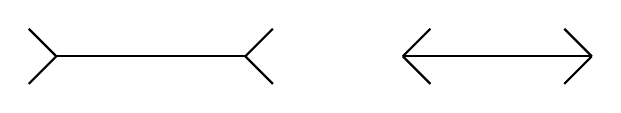
\begin{tikzpicture}[x=1cm,y=1cm]
\draw[thick] (0,0)--(2.4,0);
\draw[thick] (0,0)--(-.35,.35) (0,0)--(-.35,-.35);
\draw[thick] (2.4,0)--(2.75,.35) (2.4,0)--(2.75,-.35);
\draw[thick] (4.4,0)--(6.8,0);
\draw[thick] (4.4,0)--(4.75,.35) (4.4,0)--(4.75,-.35);
\draw[thick] (6.8,0)--(6.45,.35) (6.8,0)--(6.45,-.35);
\end{tikzpicture}
\caption{The source's Figure~1.3.1 comparison, reconstructed with equal
horizontal lengths: its left configuration can appear longer. The chapter
uses the M\"uller--Lyer illusion to distinguish a misleading appearance from
knowledge that the lengths are equal; its perspective account is one
attributed explanation, not a new perceptual experiment.}
\label{fig:p19-r13-muller-lyer}
\end{figure}

Kant's claim about necessarily Euclidean, three-dimensional perceived space
provides the other illustration. Mathematical education permits reasoning
about non-Euclidean and higher-dimensional spaces. Conceptualizing those
spaces is different from demonstrating a changed visual mechanism. The
illusion and geometry examples therefore support a distinction between
representation, judgment and reflective correction rather than a universal
genetic-determinism claim.

\section{Social cognition, language and cooperation}
\label{sec:p19-r13-social}

The source contrasts trained nonhuman symbolic signaling with human
productive syntax and proposes sociolinguistic coevolution: communication,
joint intentions, cooperation and language learning reinforce one another.
Large-prey hunting supplies its coordination example. The chapter's proposed
one-to-two-million-year genealogy is a historical evolutionary hypothesis,
not a time estimate derived from a measured sample of present infants.

Its account distinguishes cultural invention from subsequent genetic
assimilation through changed selection pressures, the Baldwin-effect
comparison. It cites Thompson--Kirby--Smith's 2016 simulations and
mathematical work against the inference that an apparently widespread
grammar necessarily requires strong innate grammatical determination.
The model's amplification claim depends on its learning and transmission
rules. No participant sample or observed historical allele trajectory is
supplied by that model attribution. The survey does not provide the full
model's equations, parameter domain or proof; its result remains a bounded
import, not a theorem about every possible learner or culture.

\subsection{Equilibrium, emergence and practical cooperation}

The chapter compares Hawk--Dove, coordination and prisoner's-dilemma
interactions. In the first, mixed behavior can be stable; in coordination
games several pure equilibria can coexist; in a one-shot prisoner's dilemma
individual defection incentives obstruct mutual cooperation. Strategy space,
payoffs, matching, repetition and dynamics determine what each statement
means. The presence of a cooperative equilibrium and its emergence from
every initial population are distinct properties.

\begin{hbexample}{def:p19-r13-stag-game}{A stated stag-hunt comparison}
Use the symmetric payoff to the row player
\[
\begin{array}{c|cc}
 &\text{Stag}&\text{Hare}\\\hline
\text{Stag}&5&0\\
\text{Hare}&3&3
\end{array}
\]
This is an illustrative model, not the original book's unspecified numerical
game. A cooperative resident earns five against another cooperative resident,
whereas a rare hare mutant earns three. Cooperation can be locally resistant
to invasion while a population with too few stag hunters favors hare.
\end{hbexample}

\begin{hblemma}{thm:p19-r13-stability}{proved=annex:p19.r13.stability}{Local evolutionary stability does not imply a global attraction basin}
In the stated game, a population with fraction \(x\) stag earns row payoffs
\(5x\) for stag and \(3\) for hare. Under the two-strategy replicator
equation \(\dot x=x(1-x)(5x-3)\), the dividing frequency is \(3/5\).
The pure stag strategy is evolutionarily stable against sufficiently rare
hare invasion, but initial \(x<3/5\) moves toward hare. Thus breakdown
after a sufficiently large change does not refute local evolutionary
stability. This repairs the source's conflation without asserting the
illustrative payoffs were its empirical inputs.
\end{hblemma}

The source's tit-for-tat example begins cooperatively and then copies the
partner's preceding action, rewarding cooperation and retaliating against
defection. Its universal-optimality reading is not adopted. The cited
Lorberbaum result has a specified repeated-game strategy and invasion
setting; it is not a universal theorem for every population structure,
noise model or sanction system. The source lists five further mechanisms:
regrouping/group selection, communication and correlated pairing,
institutional sanctions, cheater detection, and religious stabilization of
altruism. These are different hypotheses or interventions, not mutually
interchangeable demonstrations of cooperation.

Note~6 makes ``egoistic'' and ``cooperative'' evolutionary payoff roles,
not automatic diagnoses of psychological motivation. The historical contrast
between reputation in small groups and institutions in larger agricultural
communities supplies the chapter's explanatory narrative. Its references
to Hammurabi, hunter--gatherer sharing and proto-state sanctions do not
constitute a systematic dataset establishing that every known society
followed one path. Hammurabi is used as a codification example, not asserted
to be the earliest surviving juridical document.

\subsection{Mindreading mechanisms and a task-specific infant record}

The source's developmental sequence includes shared attention around nine
months, later pointing and language learning, and the ability to represent
another person's intentions and beliefs. It contrasts specialized
theory-of-mind accounts with simulation accounts that reuse machinery for
one's own attitudes to simulate another's. Evolutionary economy is an
argument for considering reuse, not evidence that fewer postulated modules
must be the actual mechanism.

\begin{hbdefinition}{def:p19-r13-onishi}{The selected 2005 nonverbal false-belief task}
Onishi and Baillargeon analyzed 56 healthy-term infants, 27 female and
29 male, mean age 15 months 7 days, range 14 months 27 days to
15 months 18 days. Another 14 tested infants were excluded: inattention
four, condition-mean outliers beyond three standard deviations four,
fussiness two, parental interference two, and observer error two.
Seven were randomly assigned to each cell of a \(2\times2\times2\)
between-infant design: actor's believed location, true/false belief,
and reached-for location. After three familiarization trials and one
belief-induction trial, test looking duration assessed expectation violation.
The belief-location by reached-location interaction was
\(F(1,48)=31.24\), \(p<.0001\); the true- and false-belief subsets also
showed that interaction. These are looking-time effects, not percentages
passing a verbal question or measurements of inherited circuitry
\cite[pp.~255--258]{R13OnishiBaillargeon2005}.
\end{hbdefinition}

The four belief histories distinguish the actor's information from the
infant's actual-location information. The authors discuss simpler last-seen
and action-expectation accounts as well as their preferred rudimentary
belief interpretation. This design is not equivalent to Wimmer--Perner's
verbal false-belief task with preschoolers. The source's age contrast does
not by itself establish one age at which every component of belief
understanding appears. Supporting methods and population-level replication
require their separate records; no new reanalysis or confidence interval
for an infant population is claimed here.

The source adds conventional moral-stage and reciprocity claims, which it
attributes to Piaget, Kohlberg and social-exchange literature. These provide
its link to generalized rules and rule-breaker detection, not a dataset
showing all children reach a fixed universal stage on their sixth birthday.
Note~7 also withdraws a strong human-exclusive intentionality claim,
mentioning chimpanzee evidence and later anticipatory eye-movement tasks.
That correction is preserved: species differences in degree and task are
not absence of every relevant capacity in every nonhuman animal.

The argument for representations then goes beyond immediate stimuli:
different perceptual cues can indicate the same behaviorally relevant object
configuration, such as a bear in a cave. A representation can mediate several
cues and several actions rather than require a distinct direct association
for each pair. Schulz's efficiency account and the source's common-cause
abduction comparison are cited explanatory proposals; economy of a model
is not alone proof that a neural system implements it.

\section{Technological control and causal models}
\label{sec:p19-r13-causal}

Sociotechnical coevolution concerns manipulating the environment as well as
predicting it: fire, stone tools, weaving, weapons and agriculture are the
chapter's examples. It distinguishes an observed association from a model
of how an intervention changes an outcome. Its three explanatory candidates
for correlated events are forward causation, reverse causation and common
causation. In a specified acyclic causal model these illustrate why an
association does not identify an intervention; they are not asserted to
exhaust every selected, cyclic or mismeasured observational record solely
from a bare Markov slogan. The actual equation-replacement interface is
\cref{def:p16-finite-scm}.

\begin{hbdefinition}{def:p19-r13-herrmann}{The selected comparative battery}
Herrmann and colleagues tested 105 German children aged 2.5 years
(\(\pm2\) months), 106 sanctuary chimpanzees aged 3--21 years,
and 32 care-center orangutans aged 3--10 years. Six scales organized
16 tasks: space, quantities and causality; social learning, communication
and theory of mind. Human experimenters administered each individual's
3--5-hour battery over several days. Table~2 reports mean physical-domain
correct proportions \(.68,.68,.59\), and social-domain proportions
\(.74,.36,.33\), in that species order. Children and chimpanzees had no
detected overall physical-domain difference; children exceeded both ape
groups socially (reported post-hoc \(p<.001\)). Physical tasks had different
chance baselines; children did better on three causal-judgment tasks while
chimpanzees did better on active stick use. The comparison was not an
equivalence test or randomized genetic intervention
\cite[pp.~1360--1366, Tables~1--2]{R13HerrmannEtAl2007}.
\end{hbdefinition}

The study discusses human-constructed tasks, experimenter species,
temperament and alternative accounts involving hidden causes. It supports
a task-pattern comparison, not a universal ``cognitive age'' for an ape or
proof of a uniquely social genetic module. The chapter's approximate
three-year comparison is kept distinct from the actual 2.5-year cohort.
Its links among pretend play, counterfactual thought and causal modeling
remain proposed mechanisms or separately cited developmental findings.

The historical intentional/physical distinction connects people interpreting
actions through goals with contact-based explanations of inanimate motion.
The source links animation of weather or celestial motion to religious
explanation, and contrasts Leibniz's intentional interpretation with Hume's
epistemic challenge. This is an attributed genealogy, not evidence that
every early explanation or every culture used an identical mechanism.

The infant illustration compares a moving ball touching another before it
moves with the second ball moving without contact; it then contrasts a boy
approaching a girl with and without touch. The chapter reports longer gaze
at the noncontact inanimate event but no corresponding difference for people,
citing Leslie and Spelke--Phillips--Woodward. Its sample, exact age range,
duration distributions and uncertainty are not supplied in this survey.
The account therefore does not establish that all six-month-olds encode
adult intentions, or that gaze uniquely identifies the proposed module.
Magnets provide the later counterexample to an unchangeable contact-only
intuition: learning a reliable action-at-a-distance pattern need not
eliminate every earlier perceptual or explanatory disposition.

\section{Modularity, generality and changing environments}
\label{sec:p19-r13-modularity}

The source's modularist account treats a module as a purpose- or area-specific
process associated with an adaptive problem, not merely a region bearing
a convenient name. Its examples include shared attention, language
acquisition, spatial models, mindreading, physical/intentional causality,
conventional moral rules and cheater detection. The cited developmental
ages are source-attributed milestones with different tasks, not one common
longitudinal panel: physical/intentional causality around six months, shared
attention around nine months, language acquisition from eighteen months,
sensorimotor spatial models over zero--two years, mindreading around
four--five years, and conventional moral values around six years. These ages
have different measures and need not identify the same onset as a nonverbal
task. The adaptive-toolbox view adds a procedure--environment
fit and the possibility that less information or computation can sometimes
be more useful.

Generalist models instead seek processes usable across problems. The source
recalls logicist expectations, later probabilistic alternatives, and task
deviations from both. Its contemporary compromise does not deny specialized
abilities: it argues that unexpected environmental change also favors
learning and reasoning not fixed to one narrow problem. The human-hand
comparison contrasts flexible reuse with a Swiss-army-knife image. Even
some evolutionary-psychology accounts admit improvisational intelligence.
The source also invokes an approximately 200,000-year evolutionary timescale
against a module for every possible task. This is its cited plausibility
argument, not a proved upper bound on the number of cognitive mechanisms.
Naming all general capacities ``modules'' would obscure the disputed
specificity rather than settle it.

Purpose-specificity and domain-specificity are nonidentical dimensions.
The chapter argues that they often covary; it supplies no sample or
correlation estimate proving a universal relation. The actual heuristic
comparison in \cref{def:p19-r24-benchmark} requires a target, available
information, resource costs and an evaluation environment. The principle,
positive theory and prescription distinction in
\cref{def:p17-br-principle-theory,def:p17-br-three-rationalities}
likewise prevents fitting a response pattern from automatically proving
a recommended procedure.

\section{Induction, method selection and the conditional examples}
\label{sec:p19-r13-inference}

Association learning is the source's most general example of inductive
projection. Its usefulness under varied tasks does not solve Hume's
justification problem. The chapter states that observations do not
deductively demonstrate the future's uniformity, and that appealing to
past inductive success would use the contested procedure. It contrasts
this with Reichenbach's best-available-method approach and Schurz's
meta-induction proposal.

The described meta-inductivist observes the performance records of accessible
methods and periodically updates a success-dependent weighted combination.
The source cites formal optimality and social-spread work; it does not
provide a complete update rule, loss convention, comparator class or horizon
in this chapter. Its all-worlds wording is therefore a source-cited relative
guarantee for a defined prediction/decision setting, not immediate
perfection, an inaccessible oracle comparison, or biological evidence that
each person uses that method. Nor is it a guarantee of transfer to hidden
feedback, an altered payoff scale or unlimited unobserved competitors.

\begin{hblemma}{thm:p19-r13-horizon}{proved=annex:p19.r13.horizon}{Long-run comparison permits an individual error}
A comparator claim \((L_T-L_T^*)/T\to0\) about cumulative losses is
compatible with a nonzero error at a finite time: the loss records
\(L_T=1\), \(L_T^*=0\) for all \(T\geq1\) have normalized gap
\(1/T\to0\). This separates an asymptotic statement's logical strength
from universal correctness on every individual problem; it is not asserted
as the full theorem of the source's meta-inductive strategy.
\end{hblemma}

The chapter distinguishes evolutionary priority from justificatory priority:
learning may precede explicit logic in phylogeny, while justifying a learning
argument still uses logical relations. Neither priority makes a psychological
implementation of a formal calculus a proved biological adaptation.
Its report of modus-ponens competence around age six, contrasted with adult
modus-tollens difficulty, is a developmental-literature attribution, not a
task-independent age-of-mastery estimate without the original records.

Its abstract four-card example uses A, B, 1 and 2 to test the rule that
A must have 1 on the other side. With a letter on one face and a number
on the other, complete falsification testing requires A and 2. B and 1
cannot expose a violation regardless of their hidden faces. This is the
renamed benchmark proved in \cref{thm:p19-r23-cards}. Choosing a card
to investigate a rule is not directly executing modus ponens or modus
tollens under an already accepted rule. A literal empirical frequency
of rule execution cannot be inferred just from a selection frequency.

The source's social regulation concerns alcohol consumption and a minimum
age of sixteen, with two beverages and two ages exposed. The counterexample
checks are the alcohol drinker and the under-sixteen person; named actors
do not change that benchmark. The source's 100/5/10/5 abstract-task
percentages and its universal-perfect social-task statement lack a recoverable
sample denominator and exact response-category definition in the chapter.
They are not adopted as new population estimates. The source Griggs--Cox
attribution concerns thematic facilitation; its task and full response tables
need their own qualified original record. The actual larger selection-task
database, with abstract/everyday/deontic denominators and limitations, is
already distinguished in \cref{sec:p19-r23-testing}.
The named adolescents and sixteen-year rule are the chapter's instantiation;
they are not asserted to be the unchanged administered materials of the
cited 1982 experiments.

The chapter favors the cheater-detection hypothesis and cites contrasts with
pragmatic deontic schemas and utility accounts, including its source-reported
claim that beneficial social exchange is important. Competing content,
familiarity, interpretation and goal effects do not vanish merely because
the hypothesis has an evolutionary explanation. The source combines that
specialization with a general probabilistic reading of uncertain ordinary
conditionals. The detailed belief-versus-frequency and conditional-query
distinctions are \cref{sec:p19-rationality-4-6}.

\begin{hblemma}{thm:p19-r13-probabilistic-mt}{proved=annex:p19.r13.probabilistic-mt}{High conditional probability does not license unrestricted probabilistic contraposition}
An arbitrarily high \(P(B\mid A)\) alone does not force high
\(P(A^c\mid B^c)\). For \(0<\epsilon<1\), put
\(P(A\cap B)=1-\epsilon\), \(P(A\cap B^c)=\epsilon\),
and both \(A^c\) cells zero. Then
\(P(B\mid A)=1-\epsilon\), but \(P(A^c\mid B^c)=0\).
Material modus tollens remains valid under its own true material-conditional
premise; these are different premise semantics, not a failure of logic.
\end{hblemma}

Thus the source's evolutionary reconciliation is a proposal about interaction:
specific social checks and broader uncertain-conditional procedures may both
be useful under different inputs and goals. The countermodel proves only
the stated probability distinction. It does not show that every participant
used conditional probability or that it uniquely explains an abstract-card
error. The actual suppression and mental-model records in Part XIX keep
the interpretation and mechanism questions distinct.

\section{The proposed architecture and its evidential standing}
\label{sec:p19-r13-architecture}

The source's conclusion gives consciousness a limited but substantial role.
Many specialized processes and some general inductive processes operate
without awareness. It rejects a purely epiphenomenal reporter view by
appealing to reflective correction, formal reasoning and institutionalized
scientific work. The road-crossing illustration contrasts rapid intuitive
estimation with slow explicit calculation, but supplies no timing experiment
or measured universal speed ratio. Scientific institutions protect some
deliberation from immediate action pressure; this is a proposed enabling
condition, not proof that reflective cognition is always superior or free
of simplification.

\begin{table}[htbp]
\centering\small
\begin{tabularx}{\textwidth}{@{}l X X@{}}
\toprule
Source level & Proposed capacity layer & Source consciousness/acquisition description \\
\midrule
Invertebrate base & Sensory and motor modules & Unconscious and innate \\
Vertebrate layer & Results of inductive conditioning & Unconscious and learned \\
Hominids/humans; primates questioned & Area-specific cognitive models/modules & Partly conscious and partly innate \\
Modern human upper layer & Universal mind/reason & Fully conscious and learned \\
\bottomrule
\end{tabularx}
\caption{All tiers and uncertainty in the source's Figure~1.3.2, represented
as a consultation table. The tiers coexist in the proposed layered account;
the animal labels are not disjoint sampled populations, and the diagram
is not a measured phylogenetic timeline or a verified partition of brain
systems. Its upper-layer wording describes the author's schematic ideal.}
\label{tab:p19-r13-architecture}
\end{table}

Euclidean geometry and perspective, formal logic and probability, relativity,
quantum theory, evolution and computing are the source's examples of cultural
achievements beyond an immediate heuristic response. The chapter's historical
names include Euclid, Leonardo, Minkowski, Aristotle, Boole, G\"odel,
Einstein, Bohr and Darwin. Its argument is for flexible general reasoning
supported by institutions and specialized representations. It is not proof
that all perceptual deception has disappeared, every intuitive error is
detectable in practice, or every modern individual's inference is optimal.

\section{Using the evolutionary account without an invalid transfer}

For consultation, distinguish an observed task effect, a model prediction,
a developmental claim, a proposed evolutionary function and an adopted
normative goal. A genetic disposition can be context-sensitive; a culturally
shared outcome can depend on learned transmission; individual success can
reflect experience rather than an independently evolved module. The present
phenotype does not identify a unique ancestral selection history. Cross-task,
cross-species and historical extrapolations require the evidence conditions
of \cref{def:p19-evidence-record}.

\begin{longtable}{@{}p{.21\linewidth}p{.33\linewidth}p{.38\linewidth}@{}}
\caption{The chapter's mechanisms and their different verification demands.}
\label{tab:p19-r13-evidence-boundaries}\\
\toprule Claim type & Source contribution & What does not follow \\
\midrule\endfirsthead
\caption[]{The chapter's mechanisms and their different verification demands (continued)}\\
\toprule Claim type & Source contribution & What does not follow \\
\midrule\endhead
\midrule\multicolumn{3}{r}{\emph{continued on next page}}\\
\endfoot
\endlastfoot
Normative criterion & Cognitive success and interest/cooperation goals are explicitly adopted. & Fitness history alone does not entail truth, welfare or an ought claim. \\
Evolutionary mechanism & Reproduction/variation/selection, cultural transmission, retention and associative induction are distinguished. & Their shared vocabulary does not establish one inheritance process or inevitable improvement. \\
Developmental observation & Verbal false-belief, looking-time, comparative battery and contact-causality examples have different measures. & A response or gaze effect does not uniquely identify an innate module or universal developmental age. \\
Strategic model & Payoffs and population dynamics explain local cooperation and invasion conditions. & A limited basin does not deny local ESS; no strategy is optimal under every unspecified repeated-game model. \\
Method comparison & Accessible success records motivate meta-inductive combination and changing-environment selection. & Relative long-run comparison is not per-trial perfection or evidence of actual ancestral implementation. \\
Reflective correction & Geometry, magnets and institutional science illustrate new representations and checking. & Correct judgment does not necessarily remove an illusion or make conscious thought invariably better. \\
\bottomrule\end{longtable}

The bibliography intake retains the source's complete reference identities
and version information, without claiming that every referenced book has
been acquired or assigning its whole contents to this treatment. The source's
historical and evolutionary proposals and the actual selected experiments
remain separately attributed. Their comparison can guide a testable account;
it does not substitute an adaptation label for evidence of its mechanism.
\nocite{Schurz2021EvolutionRationality,R13OnishiBaillargeon2005,R13HerrmannEtAl2007,R13Adams1975,R13Almor2003,R13Aunger2002,R13Axelrod2006,R13BarbeySloman2007,
R13BarkowCosmidesTooby1992,R13BarrettCosmidesTooby2007,R13Basalla1988,R13Bitterman2000,R13BlockFlanaganGuzeldere1996,R13BoydRicherson1985,R13Boyer1994,R13Brainerd1978,
R13BuchsbaumEtAl2012,R13CallTomasello2008,R13Campbell1960,R13CarruthersChamberlain2000,R13CavalliSforzaFeldman1973,R13CesaBianchiLugosi2006,R13ChengHolyoak1985,R13Chomsky1968,
R13Churchland1979,R13CosmidesBarrettTooby2010,R13CosmidesTooby1992,R13CosmidesTooby2015,R13Dawkins1987,R13DeliusJitsumoriSiemann2000,R13Dennett1995,R13Dennett2018,
R13DuchaineCosmidesTooby2001,R13Dunbar2000,R13Evans1982,R13Evans2002,R13EvansHandleyOver2003,R13Gehlen1977,R13GigerenzerSelten2001,R13GigerenzerToddABC1999,
R13GriggsCox1982,R13GurerkIrlenbuschRockenbach2006,R13Henrich2016,R13Heyes2012,R13HeyesFrith2012,R13Hume2004,R13Hume2006,R13InhelderPiaget1958,
R13JablonkaGinsburgDor2012,R13JablonkaLamb2005,R13Kahneman2011,KahnemanTversky1972Subjective,R13Kohlberg1984,R13KrupenyeEtAl2016,R13Leslie1982,R13Leslie1987,
R13Lewis1973Causation,R13Lorberbaum1994,R13ManktelowOver1991,R13Mesoudi2011,R13Millikan2002,R13NicholsStich2003,R13OaksfordChater1991,R13Over2003,
R13Papineau2003,R13Pearl2009,R13PfeiferKleiter2010,R13Piaget1932,R13RafetsederEtAl2013,R13Reichenbach1938,R13Rock1984,R13Rojas1996,
R13Schulz2011,R13Schulz2018,R13Schurz1997,R13Schurz2001,R13Schurz2008,R13Schurz2011,R13Schurz2012,R13Schurz2016,
R13Schurz2019,R13SchurzGebharter2016,R13SchurzHertwig2019,R13SchurzThorn2012,R13SchurzThorn2016,R13Skyrms2004,R13Skyrms2010,R13Sober1993,
R13SoberWilson1998,R13SpelkePhillipsWoodward1995,R13SpirtesGlymourScheines2000,R13Sterelny2012,R13Taylor1989,R13ThompsonKirbySmith2016,R13ThornSchurz2019,R13Thorndike1911,
R13ToddGigerenzerABC2012,R13Tomasello1999,R13ToobyCosmides1992,R13Topitsch1979,R13Wason1966,R13Weibull1995,R13Wenegrat1990,R13Wilson2002,
R13WimmerPerner1983,R13Woodward2003}
\index{evolution of rationality}\index{cognitive success}\index{cultural evolution}
\index{biological evolution!reasoning}\index{mindreading!task evidence}
\index{modularity!domain and purpose}\index{meta-induction!guarantee boundary}

% ED26-BM-RAT2021-1-4: exact Goel2021 chapter, printed115--126.
\chapter{Rationality and the Brain}
\label{sec:p19-rationality-1-4}

Goel's chapter asks how a brain can generate inferences while preserving
coherence among beliefs and proposed actions. Its answer is not a single
reasoning organ: it proposes several systems for inference generation,
together with a more general system for handling conflict. The proposed
division depends on conceptual versus logical relations, logical form,
familiar content, presentation modality and determinacy
\cite[pp.~115--124]{Goel2021RationalityBrain}.

The evidence and the interpretation must be distinguished. A contrast in
neural activity is an observation under a particular task and baseline;
assigning it an inferential function is a further claim. Lesions and
stimulation add different constraints, but neither automatically establishes
an isolated, necessary-and-sufficient reasoning module. The chapter's own
note~4 says that the experiments have not clearly separated conflict
\emph{detection} from conflict \emph{resolution}. The account below preserves
that qualification rather than treating two names as two established stages.

The source is the complete 2021 chapter~1.4, not the 2012 Oxford chapter~6.
The two independently inspected empirical anchors are Goel and colleagues'
2007 lesion study and Prado, Chadha and Booth's 2011 imaging meta-analysis.
Other original-study findings are explicitly presented as reports in the
selected chapter. Their missing participant, task, stimulation, analysis or
uncertainty records are not filled with invented details. No new neural
experiment, participant-level reanalysis or population prevalence estimate
is reported here. The reporting interface is
\cref{def:p19-evidence-record}.

\section{Rational action, represented belief and coherence}
\label{sec:p19-r14-criteria}

\begin{hbdefinition}{def:p19-r14-functional-problem}{The source's functional problem}
In Goel's instrumental account, a rational action is a deliberate action
selected from a large or potentially unbounded set of possibilities that advances an organism's
goals coherently with its knowledge and beliefs. A \emph{veridical} belief
fits the world; coherence concerns relations among represented beliefs,
inferences and actions. Neither relationship is identified with a brain
region or with the frequency of a response.

The source distinguishes five requirements: obtaining beliefs that fit the
world; maintaining them in memory; generating inferences; detecting
inconsistency; and updating or revising beliefs. The present neural account
focuses on inference and consistency maintenance. Perception and memory
are required interfaces, not mechanisms fully explained by this account.
\end{hbdefinition}

The thirsty person who believes that a glass of water is on the right of
the desk has a reason to reach right. Reaching left while retaining that
belief is the source's contrasting incoherent action. This example assumes
the thirst-relief goal and the represented location; it is not a universal
claim that leftward movement is irrational. In note~1 the author adds a
philosophical claim, attributed to Cassirer, that antecedent conditions do
not causally suffice for the ensuing rational action. That claim is not a
result of the neural experiments. Note~2 treats epistemic evaluation as
instrumental rationality applied to beliefs and revision. This is Goel's
choice of framework, not a demonstration that all distinctions between
epistemic and practical standards disappear
\cite[pp.~115--116, 124, notes~1--2]{Goel2021RationalityBrain}.

Beliefs, rather than the world directly, mediate the source's action
examples. Believing that a dangerous tiger is under the desk can prompt
flight even when no tiger is there; the same action can be apt if the
belief is true. Conversely, coherent action based on a false location
belief can miss the water. Coherence and veridicality can therefore come
apart. Whether a particular false belief causes harm also depends on the
remaining beliefs, action policy and circumstances; inconsistency alone
does not force a person to enact every conflicting prescription.

\paragraph{Conceptual and logical relations.}
Semantic knowledge supports the connection between being a widow, being a
woman and having had a husband who died, in the source's usage. Logical
connectives and quantifiers constrain patterns involving conjunction,
disjunction, conditionals, universality and existence. Relational expressions
such as greater-than or inside need their own interpretation. The example
that George is taller than Michael and Michael is shorter than George
expresses a relation and its converse. Goel uses such intuitively compelling
connections to explain coherence and regards coherence as primitive. His
description of them as unprovable is not a mathematical impossibility claim:
in a formal language that defines shorter-than as the converse of
taller-than, the connection follows from that definition. The reader must
keep an intuitive psychological starting point separate from the declared
first-order semantics of \cref{sec:fol-semantics-02}
\cite[pp.~115--117]{Goel2021RationalityBrain}.

Induction from observed dogs to unobserved dogs having tails and the causal
explanation of seasons by the Earth's axial tilt illustrate other relations
used in inference. They do not become logical consequences merely because
they are familiar. Sampling, causal assumptions and background knowledge
matter. The source's evolutionary rationale---inference and inconsistency
handling serving truth preservation---is an explanatory proposal, not a
proof that an evolved inductive procedure preserves truth in every case.
The corresponding distinction between evolutionary success and adopted
evaluative criteria is developed in \cref{sec:p19-rationality-1-3}.

\paragraph{The swan revision and its boundary.}
Seeing twelve white swans at Lake Simcoe can lead to the hypothesis that
all swans are white. A later black swan contradicts that universal
hypothesis. The chapter illustrates revision by replacing it with a
most-swans claim. The logically warranted correction from this new
observation is only that \emph{not all} swans are white. It is not that
every swan is nonwhite, and one counterexample does not establish that
most are white. A majority claim needs additional population and sampling
information. This separates successful inconsistency detection from the
adequacy of the particular revision selected
\cite[p.~116]{Goel2021RationalityBrain}.

The chapter deliberately does not explain delusions; note~3 argues for
first understanding ordinary rationality. Its examples consequently cannot
be transferred into a diagnosis of a psychiatric condition. Nor does the
restriction turn neurological patient data into a sample of all ordinary
reasoners \cite[p.~124, note~3]{Goel2021RationalityBrain}.

\section{Inference generation: interpreter, induction and analogy}
\label{sec:p19-r14-generation}

Prefrontal cortex is abbreviated PFC; a Brodmann area is abbreviated BA.
These are anatomical designations, not labels for inference rules. Goel
does not adopt a mental-logic, mental-model, dual-system or probabilistic
theory wholesale before organizing the neural evidence. His proposed
left-PFC interpreter is sensitive to linguistic and conceptual relations;
other frontal and parietal systems contribute to more formal processing,
with a right ventrolateral-PFC contribution to indeterminacy. The proposal
is an organization of the evidence, not a literal implementation of a
specified formal calculus \cite[pp.~117--118]{Goel2021RationalityBrain}.

\paragraph{The split-brain illustration.}
In the Gazzaniga example reported by Goel, a chicken claw is presented in
the right visual field and a snowy scene in the left. The participant's
right hand selects a chicken picture, while the left selects a shovel.
The language-dominant left hemisphere, lacking access to the snow scene,
explains the shovel as useful for cleaning the chicken coop. The proposed
interpreter makes a coherent explanation from the information available
to it, without thereby recovering the actual cause of the other selection.
The visual fields, hand responses, disrupted interhemispheric access and
verbal report are essential to the example. It is not evidence that every
normal explanation is confabulated, nor that the left PFC alone suffices
for rationality. The chapter attributes the demonstration to Gazzaniga
1989 and the interpreter discussion to his 1998 book; it does not supply
the original case sample, recruitment or uncertainty record
\cite[p.~117]{Goel2021RationalityBrain}.

\paragraph{Belief-based induction.}
The description of forty-two-year-old Eve as serious and orderly, enjoying wine and chess and
watching foreign television news can make librarian seem more plausible
than football player. That assessment, attributed to the heuristics
literature, is not an entailment or a verified occupational probability.
Its stereotypic content must not be adopted as a fact about the person.
Similarly, snakes and alligators being cold-blooded does not entail that
all reptiles are cold-blooded. The induction studies of Goel and colleagues
1997 and Goel--Dolan 2004 are reported to engage left dorsolateral PFC,
including BA~9, 8 and 45; the source distinguishes induction from its
deductive comparison by greater left middle-frontal activity around BA~9
\cite[p.~118, fig.~1.4.1a]{Goel2021RationalityBrain}.

The 2019 focal-lesion study varies conclusion believability. Its examples
range from generalizing the residence of one German shepherd to all such
dogs living in D\"usseldorf, through an inference from the glossiness and
moistness of lipstick and fish scales to lipstick containing fish scales,
to the highly believable reptile conclusion. Goel reports less entrenched
beliefs and less acceptance of moderately or highly believable conclusions
following unilateral left BA~9/10 damage. A less believable response is
not automatically a worse inference; acceptance intensity, factual
accuracy and justification are distinct outcomes. The original patient
counts, lesion overlap, response scale and statistical uncertainty remain
unqualified in this source-level report
\cite[p.~118]{Goel2021RationalityBrain}.

\paragraph{Analogical mapping is not one task.}
The chapter juxtaposes three paradigms. Wharton and colleagues' 2000
colored-shape mapping task contrasts analogy with literal identity and
is associated with medial frontal, extensive left prefrontal, anterior
insular and left inferior-parietal activity. Green and colleagues' 2006
word analogy, planet:sun as electron:nucleus, is associated with left
superior frontal BA~9/10 and a frontal-parietal network. Luo and colleagues'
2003 verbal analogy, soldier:army as drummer:band, is reported to involve
bilateral PFC, left temporal cortex and hippocampus. These are different
stimuli and comparisons. Their overlapping activity supports neither
identity of the cognitive operations nor a single analogy locus. No
original-study sample or effect size is supplied by the selected chapter
for these examples \cite[p.~118]{Goel2021RationalityBrain}.

\section{Logical form and belief-laden content}
\label{sec:p19-r14-logical-forms}

Here \(A,B,C\) are temporary schematic names, not measured brain states.
The source contrasts categorical inclusion, transitive comparison,
conditional inference and disjunction. For categorical arguments, all
\(A\)s being \(B\)s and all \(B\)s being \(C\)s entails all \(A\)s
being \(C\)s under the ordinary inclusion interpretation. For a transitive
strict ordering, \(A>B\) and \(B>C\) entails \(A>C\). For the chapter's
deductive conditional benchmark, if Saturday rain rules out Linda's
barbecue and rain occurs, the barbecue is ruled out. For a classical
disjunction, Tom attending with Linda or Mary and not attending with Mary
entails attending with Linda. These benchmarks require their stated
interpretations; an everyday defeasible conditional is not silently
replaced by material implication
\cite[pp.~118, 120]{Goel2021RationalityBrain}.

Goel's broccoli--vegetable--green example has a valid categorical form
even if its universal vegetable premise is false. His London--Paris--Rome
example uses a transitive north-of ordering as a task premise, not a new
geographical measurement. Replacing familiar words by letters preserves
the intended form while changing the content available to a reasoner.
Validity, perceived believability and response accuracy must therefore
be coded separately, as in \cref{sec:p19-rationality-2-3}.

\begin{center}
\begin{tabular}{@{}p{0.09\textwidth}p{0.53\textwidth}p{0.25\textwidth}@{}}
\toprule
Source case & Premises and conclusion & Deductive/content contrast\\
\midrule
H & All broccoli are vegetables; all vegetables are green;
therefore all broccoli are green. & Valid form; source's believable
conclusion.\\
N & No apples are fruit; all fruit contain calories;
therefore no apples contain calories. & Invalid; source's unbelievable
conclusion.\\
O & All apples are fruit; all fruit are poisonous;
therefore all apples are poisonous. & Valid; source's unbelievable
conclusion.\\
P & No apples are fruit; all fruit contain calories;
therefore all apples contain calories. & Invalid; source's believable
conclusion.\\
\bottomrule
\end{tabular}
\end{center}
The table reconstructs the source's congruent cases H/N and incongruent
cases O/P, rather than asserting the truth of its stipulated premises.
For N and P, apples can be disjoint from fruit while being either
calorie-containing or calorie-free. Those two interpretations both satisfy
the premises and separate the proposed conclusions. Believability is a
participant-related content classification; it is not another validity
relation \cite[pp.~120--121]{Goel2021RationalityBrain}.

\paragraph{Form-sensitive neural reports.}
The chapter's quantitative anchor associates categorical reasoning with
left prefrontal BA~9/44, left precentral cortex and basal ganglia;
transitive reasoning with bilateral parietal and dorsal frontal areas;
and its conditional discussion with left dorsal frontal and angular-gyrus
activity. Individual syllogistic studies include Goel 2000, Goel--Dolan
2003 and Reverberi 2012; Reverberi and colleagues' 2009 lesion report
implicates left lateral and superior medial frontal regions in elementary
deduction. The linguistic transitive literature includes Knauff and
colleagues 2003 and Modro\~no and colleagues 2018, and the disjunctive and
conditional examples refer to Eimontaite 2018 and Noveck 2004. These are
source-reported task associations, not evidence that any BA contains a
named logical connective. The source itself regards the smaller conditional
literature as less robust and notes Baggio and colleagues' 2016 left
BA~44/47 findings \cite[pp.~118--120]{Goel2021RationalityBrain}.

\paragraph{Content contrasts and patient constraints.}
For categorical syllogisms, the selected chapter reports left
frontal-temporal involvement for familiar meaningful content and bilateral
PFC, parietal and occipital involvement for corresponding abstract material,
with content controls in Goel 2000 and Goel--Dolan 2003. For familiar
geographical transitive arguments, Goel, Makale and Grafman 2004 report
left parahippocampal and bilateral hippocampal involvement; abstract
counterparts involve bilateral parietal cortex. The controls and baselines
matter: the reported contrast is not a subtraction of one pure reasoning
faculty from another \cite[p.~121, fig.~1.4.1b--f]{Goel2021RationalityBrain}.

Vartanian and colleagues' 2009 frontotemporal-dementia report is a useful
boundary case: relatively spared parietal regions accompany preserved
abstract transitive performance but impaired familiar-content performance.
Goel, Shuren, Sheesley and Grafman's 2004 focal-lesion Wason study reports
similar performance to controls on the arbitrary task but a missing
familiar-content benefit, driven particularly by the left-PFC patients.
Preservation on one version does not imply preservation of every reasoning
capacity. Neither dementia nor a focal-lesion group is randomly assigned
to an anatomical condition. The original samples, lesion distributions,
task scoring and uncertainty for these two reports remain open here
\cite[p.~121]{Goel2021RationalityBrain}.

The rTMS findings reported from Tsujii and colleagues 2010/2011 sharpen
the distinction: left-PFC disruption affects congruent content trials,
not all contentful trials alike. Goel therefore proposes a more restricted
left-PFC contribution through belief bias, conceptual connections and
simple connectives, with other resources needed for complex logical
relations. His possible necessary-and-sufficient interpretation of left
PFC for familiar congruent inference is stronger than the task contrast
alone establishes. A disruption effect can implicate an essential
contribution within a network without showing that the stimulated region
is independently sufficient \cite[p.~121]{Goel2021RationalityBrain}.

\section{The quantitative imaging anchor and its alternatives}
\label{sec:p19-r14-meta}

\paragraph{Corpus, people and comparisons.}
Prado, Chadha and Booth analyzed 28 published peer-reviewed fMRI/PET
studies from 1997--2010, combining 382 participants. Eligibility required
healthy adults, whole-brain activation coordinates in MNI or Talairach
space, and a deductive-reasoning-versus-baseline contrast. Goel's 2007
review provided the initial corpus; PubMed and ScienceDirect searches
covered May 2007--September 2010. Goel--Dolan 2003 was not included because
the required reasoning-versus-baseline coordinates were not reported.
The corpus is not a random sample of all people or all reasoning tasks
\cite[pp.~3484--3488, table~1]{PradoChadhaBooth2011DeductionMeta}.

The selected baselines include sentence comprehension, matching,
nonintegrable premises, fixation, and simpler reasoning. Some contrasts
therefore estimate reasoning against a nonreasoning activity, others the
increment from a simpler to a more complex argument. Material, input
modality, training, imaging method and analyzed phase also vary. The
authors did not have enough studies to examine all those factors
separately. Their three categories are \emph{relational}, \emph{categorical}
and \emph{propositional}. The last includes conditional and disjunctive
inferences, including different forms such as modus ponens and modus
tollens. It must not be renamed a homogeneous conditional-task corpus.

\paragraph{Analysis and reported uncertainty.}
Multilevel kernel density analysis convolves reported peaks with a
10-millimetre-radius sphere and aggregates contrast maps, rather than
counting every peak as an independent participant. Weighting uses the
square root of sample size and an analysis-type multiplier, 1 for
random-effects and 0.75 for fixed-effects analyses. Monte Carlo simulation
with 5,000 iterations supplies the whole-brain threshold; results are
reported at \(p<0.05\), family-wise-error corrected. The target is
spatial consistency of reported activation around a location relative
to the declared spatial null, not the probability that a person uses
a particular cognitive algorithm. No neural effect-size interval or
participant-level reanalysis is manufactured here
\cite[pp.~3485, 3488]{PradoChadhaBooth2011DeductionMeta}.

Across the corpus the reported network is predominantly left
fronto-parietal with basal-ganglia involvement. Category-specific analyses
and direct category contrasts are different results. Relational tasks
consistently involve bilateral posterior parietal and right middle frontal
regions; categorical tasks involve left inferior frontal and basal-ganglia
regions; propositional tasks involve left posterior parietal, precentral
and medial frontal regions. Only left precentral cortex distinguishes
propositional tasks from both other categories in the reported direct
contrasts. For relational tasks, bilateral posterior parietal activity
persists when the five nonlinguistic studies among the eleven relational
studies are removed. Thus visual/nonlinguistic presentation does not
by itself explain the parietal finding
\cite[pp.~3489--3494, tables~2--3]{PradoChadhaBooth2011DeductionMeta}.

\paragraph{What remains a mechanism hypothesis.}
The meta-analysis interprets linear orderings as comparatively easy to
map onto a spatial continuum, while set-inclusion premises allow multiple
configurations and may encourage rule-based representations. Its
propositional result is less decisive: angular-gyrus activity can reflect
verbal as well as spatial processing, medial frontal activity can relate
to abstract-rule maintenance, and precentral activity can reflect
attention or motor demands. The authors explicitly acknowledge that
region-to-process inference lacks a one-to-one mapping and cannot
definitively identify visuospatial versus syntactic computation
\cite[pp.~3492--3494]{PradoChadhaBooth2011DeductionMeta}.

This is a substantive alternative to simply declaring all imaging
findings inconsistent. The source compares meaningful task-dependent
fractionation with methodological differences and with a proposed
left-rostrolateral/medial-frontal deductive core from Monti's studies.
It does not find those proposed core regions consistently across all
tasks; integrating several logical relations in complex tasks is an
alternative explanation for their involvement. Different distributions
of activity constrain a uniform-localization account. They do not,
without a linking theory, prove that no common abstract operation is
implemented in differing networks or that a behavioral model has been
formally refuted. Multiple strategies, individual skills and shared
encoding, memory, control and response operations remain alternatives
\cite[pp.~3494--3495]{PradoChadhaBooth2011DeductionMeta}.

\section{Presentation modality and indeterminacy}
\label{sec:p19-r14-modality}

The chapter contrasts linguistic transitive tasks, usually associated
with parietal involvement, with the pictorial tasks of Fangmeier and
colleagues 2006 and Wendelken--Bunge 2010, associated with anterior or
rostrolateral right BA~10. Waechter and colleagues 2013 propose that
linguistic stimuli must be mapped onto a spatial representation, whereas
the picture already exemplifies the relation. The resulting difference
in representational preparation is an explanatory hypothesis, not a
within-participant modality effect measured by juxtaposing separate
studies. The chapter also reports their lesion comparison: parietal
damage impairs transitive rather than categorical performance. Neither
finding establishes that every pictorial task bypasses parietal cortex
\cite[pp.~120, 122]{Goel2021RationalityBrain}.

The proposed mapping explanation draws on Johnson-Laird's mental models,
Mani--Johnson-Laird's spatial-description work, Cohen and colleagues'
mental-rotation imaging, Goel--Dolan 2001 and Knauff and colleagues 2003.
These interfaces are not interchangeable. In
\cref{sec:p19-mental-rotation}, rotation time can include encoding,
comparison and response components; it does not directly reveal a unique
representation. Likewise, parietal activity during linguistic inference
does not directly reveal a literal internal picture. The current
psychological model account is \cref{sec:p19-rationality-2-3}, not the
model-theoretic meaning of a structure satisfying sentences.

\paragraph{Determinate, inconsistent and unsettled conclusions.}
The source's population example contrasts Toronto larger than Hamilton
and Hamilton larger than Guelph with Toronto larger than each of the
other cities. The first pair determines Toronto larger than Guelph. The
second pair does not determine the Hamilton--Guelph ordering. Under a
strict numerical ordering, take Toronto's value as 3 and the other two
values as 2 and 1 in either order; both assignments satisfy the second
pair but disagree about which of Hamilton and Guelph is larger. Giving
both value 1 supplies a third possibility. This is indeterminacy
\emph{relative to the premises}, not absence of an actual population fact.
It also is not contradiction: both premises can be true
\cite[p.~122]{Goel2021RationalityBrain}.

Rejecting an unentailed conclusion can therefore mean either that it
contradicts the premises or that it remains compatible but unsettled.
The same binary response does not identify the same psychological
operation. Goel reports right-PFC effects for indeterminate relations
from the 2007 patient study, Goel and colleagues 2009 and Brzezicka and
colleagues 2011 imaging, and an indeterminate-syllogism result from
Parsons--Osherson 2001. Ragni and colleagues' 2016 stimulation study
implicates right superior parietal cortex in uncertain spatial reasoning,
but did not test right PFC. It is not a direct replication of the
right-PFC localization \cite[p.~122]{Goel2021RationalityBrain}.

\section{A full primary lesion evidence record}
\label{sec:p19-r14-lesion-record}

\paragraph{People, design and anatomical measurement.}
Goel and colleagues' 2007 study compares nine left-PFC patients, nine
right-PFC patients and 22 age/education-matched controls. Selection
required focal unilateral prefrontal lesions and relatively intact
sensory, motor, language and cognitive functions. Thirteen patients had
Vietnam-era penetrating injuries and were tested in 1999--2002. The five
others had two tumor excisions, an aneurysm and two strokes, with differing
post-injury intervals. Mean ages were 48.50, 54.38 and 49.00 years for
left, right and control groups respectively; mean education was 15.00,
14.67 and 14.84 years. This is a selected clinical comparison, not
randomized damage or a population survey
\cite[pp.~2245--2247, table~1]{GoelEtAl2007CertainUncertain}.

Lesions were traced before behavioral testing from MRI/CT, registered to
a template and compared with approximate BA labels. Damage is not confined
to one BA; BA~10 was involved in eight right and seven left patients,
and the reported group-average losses by BA did not significantly differ.
The printed overlay figure covers fifteen patients, whereas the behavioral
sample is eighteen. The main paper refers to supplementary individual
maps and a supplementary table, which are not supplied by the held
six-page main PDF. The anatomical record cannot be treated as a complete
inspection of all eighteen individual maps.

\paragraph{Task and denominator.}
Participants classified self-paced, visually presented three-term
arguments as valid or invalid using two keys, after a validity explanation
and examples. There were two blocks of 51 trials, with rests after every
25. Half the materials were spatial relations, such as ahead-of; half
were nonspatial relations, such as smarter-than, treated by the study
as orderable relations. The authors collapsed them after reporting
similar accuracy, 71 versus 72 percent, with \(p=0.67\). That decision
does not demonstrate equivalence of their cognitive processes.

The final item counts are 52 valid determinate, 28 inconsistent
determinate and 22 indeterminate, totaling 102. The paper expressly
reports stimulus misclassifications responsible for departures from the
intended balance. Indeterminate trials require ``invalid,'' not a third
uncertainty key. They are not economic risk/reward choices or conditional
probability estimates \cite[p.~2247]{GoelEtAl2007CertainUncertain}.

\paragraph{Results and uncertainty.}
Overall accuracy is reported as 76 percent, SD 15 percentage points.
With education as covariate, the three-group-by-determinacy analysis
reports \(F_{2,33}=6.82\), \(p<0.01\). On determinate items the means
are 72.0 percent for left patients, 78.8 for right patients and 84.7 for
controls; corresponding SDs are 17.6, 11.0 and 14.2. On indeterminate
items the means are 73.5, 56.1 and 79.0, with SDs 19.8, 22.5 and 18.4.
The left-versus-right determinate comparison is explicitly one-tailed
under the stated prior hypothesis. These SDs describe variability of
scores, not confidence intervals for a group difference
\cite[pp.~2247--2248, fig.~2]{GoelEtAl2007CertainUncertain}.

IQ, general and working memory, fluency and naming scores were correlated
with task performance. A second analysis enters six covariates in the
patient-only comparison because the corresponding control scores were
unavailable; it reports an interaction \(F_{1,8}=13.10\), \(p<0.01\).
This adjusted clinical comparison does not establish that every relevant
confound was measured or that all patients used the same strategy.

\paragraph{A separating check on response bias.}
Determinate items mix yes and no responses; indeterminate items all
require no. The authors therefore reanalyze valid, inconsistent and
indeterminate items separately, reporting a lesion-by-item-type
interaction \(F_{2,16}=7.46\), \(p<0.01\). Right versus left accuracy is
56.1 versus 73.5 percent on indeterminate items, 79.8 versus 71.5 on
valid determinate items, but 76.6 versus 75.8 on inconsistent determinate
items. The last comparison is particularly important: it does not fit
an explanation in which right damage simply impairs every no response
or every inconsistency judgment. The source regards response balance
as insufficient to explain the crossover. No new equivalence test or
interval for the near-equal inconsistent means is inferred here
\cite[p.~2248]{GoelEtAl2007CertainUncertain}.

\paragraph{Mechanism and unresolved alternatives.}
The authors propose that right PFC supports maintaining an ambiguous
representation, tempering the left interpreter's premature commitment.
They consider additional working-memory/attention demands as an
alternative, arguing against a simple load account using baseline
scores, covariates, lesion overlap and other imaging observations.
Those arguments narrow alternatives without directly measuring the
postulated ambiguous representation. Their extension to gambling-task
set changes is an explanatory proposal, not a gambling experiment
conducted in these 40 participants. The claimed one-third error
consequence of choosing a specific interpretation also needs an
assumption about how alternatives are selected; it is not a logical
consequence of indeterminacy alone
\cite[pp.~2248--2249]{GoelEtAl2007CertainUncertain}.

The 2021 chapter describes left lesions as producing generalized
impairment and right lesions as selectively impairing incomplete
information. The main 2007 record more specifically supports a
crossover between valid determinate and indeterminate performance,
with similar inconsistent-item means. This preserves the clinical
finding without broadening it into every inferential operation
\cite[p.~122]{Goel2021RationalityBrain}.

\section{Conflict handling is not identified by the final answer}
\label{sec:p19-r14-conflict}

In incongruent syllogisms, an answer cued by conclusion believability
can oppose the validity benchmark. The selected chapter associates
belief-biased responses with ventromedial PFC BA~11/32 and successful
conflict handling with right lateral/dorsolateral PFC, while parietal
resources contribute to formal evaluation. Its cited reports include
Goel 2000, Goel--Dolan 2003, De Neys--Vartanian--Goel 2008,
Prado--Noveck 2007 and Stollstorff--Vartanian--Goel 2012
\cite[pp.~122--123]{Goel2021RationalityBrain}.

A correct answer is compatible with detecting conflict, inhibiting
a belief-driven response and generating a formal response, but it does
not alone observe that entire sequence. A participant can answer by
another strategy, and a wrong answer can follow detection without
successful resolution. This is why the source's explicit detection/
resolution uncertainty matters. Nor does every internally inconsistent
belief set produce conscious conflict on every trial.

\paragraph{Stimulation contrasts.}
As reported by the chapter, right-PFC rTMS impairs incongruent
performance, whereas left-PFC disruption impairs congruent performance
but can improve incongruent performance. The interpretation is that
disrupting a content-sensitive route can reduce irrelevant semantic
interference, permitting other resources to determine the answer.
The intervention contrast does not make impairment a universal decrement
in rationality. For the original Tsujii 2010/2011 reports, sample sizes,
coil placement, stimulation protocol, control/sham conditions, order,
assignment, effect magnitudes and uncertainty are not fully qualified
here; the chapter's reported directions are not a completed intervention
record \cite[p.~123]{Goel2021RationalityBrain}.

\paragraph{Lesion and rule-induction contrasts.}
Caramazza and colleagues' 1976 two-term task asks who is taller and who
is shorter after a taller-than premise. Goel reports widespread left
hemisphere impairment but a right hemisphere deficit for the question
requiring the converse relation. This is a polarity/representation
contrast, not a contradiction in the premise itself. Reverberi and
colleagues' 2005 revised Brixton task separates induction of a rule
from coping with rule conflict; the chapter reports left-PFC impairment
in induction and right-PFC impairment in conflict. These tasks are not
identical to belief--logic incongruence. Their original clinical and
uncertainty records remain unqualified here
\cite[p.~123]{Goel2021RationalityBrain}.

The broader generalization cites Fink 1999, Picton 2006, two Vallesi
2007 reports, and Marinsek 2014. They contribute different intention,
timing, temporal-preparation and hemispheric paradigms, not repeated
instances of the same deductive task. Hamburger and colleagues 2018
and Knauff's spatial-reasoning account supply a related case in which
visual imagery can interfere with spatial reasoning; they do not
identify every visual or right-PFC operation as conflict detection.
Without their task-specific records, these citations support attribution
of the source's generalization rather than a new cross-paradigm effect
estimate \cite[p.~123]{Goel2021RationalityBrain}.

\section{Localization, causal interpretation and neural plausibility}
\label{sec:p19-r14-limits}

The chapter's figure collects nine panels from distinct studies. Panels
a--h concern induction, meaningful syllogisms, abstract syllogisms,
familiar and abstract transitive relations, pictorial integration and
indeterminate relations; panel~i concerns conflict handling. It is not
a factorial experiment in a single sample. Its caption labels the
conflict panel BA~44/45, while the later text gives BA~45/46. The
qualitative right lateral/dorsolateral attribution can be preserved,
but those differing anatomical details cannot be silently reconciled
into a new precise locus without the original imaging record
\cite[p.~119, fig.~1.4.1; p.~123]{Goel2021RationalityBrain}.

Three inferential boundaries are consequential. First, a measured
signal can covary with a condition containing encoding, representation,
memory, inference, control and motor response; it is not a direct readout
of one process. Second, disrupting a region can affect connected
systems and a particular task contribution; an effect does not show
that the region alone computes the inference. Third, lesion groups
can differ in history, extent, preserved resources and compensation;
adjustment and dissociations constrain those alternatives but do not
turn the design into random anatomical assignment. These are reasons
to triangulate task contrasts, behavior, imaging and intervention,
not reasons to discard neural evidence.

The mapped 2012 Oxford chapter, Morrison--Knowlton's \emph{Neurocognitive
Methods in Higher Cognition}, concerns what neural measurements and
interventions can establish about a reasoning mechanism. Its mapped
questions include behavioral underdetermination, neuropsychological
cases, EEG/fMRI measurements, TMS and prefrontal cognition. That is a
methodological comparison interface, not another edition of Goel's
2021 multi-system account. Its full chapter is not qualified by the
present source corpus, so no uninspected Oxford argument or completed
coverage credit is supplied here. The present lesion and imaging
records illustrate the questions at that interface without replacing
the missing Oxford treatment.

The existing P19 dual-process account requires specification of
representations, computations, engagement and interactions
(see \cref{def:p19-r25-process-account,def:p19-r25-interactions}). Goel's
interpreter/formal/conflict organization is not a direct anatomical
identification of Type~1 and Type~2. A belief-based route can be correct,
a resource-demanding route can err, and multiple neural resources can
contribute to one response. Likewise, the task/construct/measure
distinction in \cref{def:p19-empirical-question} rules out declaring a
participant rational from an activation label. An empirical neural
constraint does not establish the normative benchmark against which
the response is judged.

\section{Using the account for an actual reasoning question}
\label{sec:p19-r14-use}

To evaluate a proposed neural explanation, first state the argument
interpretation and response criterion; then separate form, content,
modality, determinacy and conflict. Record the people, comparison,
measurement or perturbation, baseline and reported uncertainty. Ask
which competing mechanism would produce the same score or signal.
The success case is the 2007 lesion contrast: the indeterminate deficit
is compared with valid and inconsistent determinate items, so a simple
no-response explanation can be tested against the actual pattern.
The failure case is to infer a unique uncertainty mechanism merely
from a right-frontal activation, or to infer a general loss of
rationality merely from a focal clinical deficit.

Goel's conclusion is a provisional multi-system account: linguistic/
conceptual inference, form- and modality-sensitive visuospatial
resources, indeterminacy tolerance and more general conflict handling
cooperate in maintaining a useful belief network. The source expects
the anatomical and functional details to change with further evidence.
Its broad rejection of a unitary reasoning module is an empirical
interpretation of the reviewed studies, not an impossibility theorem
about all common computations. Correctness of a formal inference,
accuracy of a belief, observed clinical performance and rationality
under adopted goals remain four different questions
\cite[pp.~123--124]{Goel2021RationalityBrain}.

% ED26-BM-RAT2021-6-2: Over--Cruz's exact 2021 chapter, pp. 395--404.
\chapter{The Suppositional Theory of Conditionals and Rationality}
\label{sec:p19-rationality-6-2}

Over and Cruz's account concerns principally singular, natural-language
indicative conditionals: what happens on the next toss, or on this afternoon's
journey, rather than a universal rule about every member of a domain.
Its central proposal is that assessing ``if \(A\), then \(B\)'' amounts to
assessing \(B\) while supposing \(A\). The associated degree of belief is
the subjective conditional probability \(P(B\mid A)\). The authors propose
both a normative standard and a descriptive hypothesis. Probability-theoretic
coherence supplies the former; correspondence between conditional judgments
and conditional probabilities supplies the latter. A descriptive fit does not
establish the normative premise, and endorsing that premise does not entail
that people always comply with it \cite[pp.~395--401]{OverCruz2021Suppositional}.

\section{The account and the prediction to be tested}
\label{sec:p19-r62-account}

\begin{hbdefinition}{def:p19-r62-equation}{The suppositional account and its two claims}
Write \(P(\text{if }A\text{ then }B)\) for the subject's assessment of
the ordinary-language conditional, without presupposing that it is the
probability of a fixed Boolean event. The \emph{Equation} is
\[
 P(\text{if }A\text{ then }B)=P(B\mid A).
\]
The chapter's normative proposal assesses reasoning with that interpretation
by coherent subjective probability. Its \emph{conditional probability
hypothesis} predicts that people's judgments of the conditional will
correspond to their judgments of \(P(B\mid A)\). This is a prediction
about a specified elicitation task, not a definition of the observed response.
For the finite calculations below, ratio conditioning requires \(P(A)>0\).
The psychological operation of supposing an antecedent is not defined by
division by zero when that condition fails.
\end{hbdefinition}

The historical foundations invoked are Ramsey's 1926 and 1929 writings,
de Finetti's 1936 and 1937 work, and Edgington's development of the Equation.
The chapter also calls its conditional a probability conditional or
conditional event. Those names identify an interpretation here, not an
automatic adoption of every axiom for iterated conditional random quantities
in \cref{sec:p15-rationality-4-4}.

Reasoning from \(A\), together with background beliefs, to \(B\) can
support a conditional assertion; the assertion can in turn summarize that
reasoning. The authors' unification proposal therefore places conditional
probability at the interface between reasoning, judgment and decision making.
It is a research program, not a completed theorem equating every cognitive
task or every aspect of rationality. Cognitive limitations and fallacies are
compatible with the descriptive hypothesis. The authors predict that
probability theory will describe conditional reasoning more accurately
than binary extensional logic. That comparative proposal needs matched
tasks and model versions; it is not established for every task by the
Equation's definition.

The source reports corroboration across Evans--Handley--Over (2003),
Evans--Handley--Neilens--Over (2007), Oberauer--Wilhelm (2003),
Over and colleagues (2007), Pfeifer--Kleiter (2005), Fugard and colleagues
(2011), and Singmann--Klauer--Over (2014). Its review does not provide those
studies' complete recruitment, exclusions, response distributions or
uncertainty estimates. The original-study records in
\cref{sec:p19-rat46-interpretations,sec:p19-r45-coherence-studies} retain
their own tasks and denominators; they are not pooled into a population
frequency by this list of corroborating citations.

\begin{hbexample}{def:p19-r62-singular-general}{A bird rule is not a next-animal prediction}
The assertion that birds fly, read as a general conditional covering its
whole domain, has counterexamples. A prediction that the next animal seen
will fly if it is a bird can nevertheless be highly credible in a suitable
setting. Its credibility depends on the local distribution and background
knowledge. The chapter confines its main treatment to singular conditionals,
referring the comparison of ``if'' with ``all'' to Cruz--Oberauer (2014).
Success on one task does not establish a semantics for the other.
\end{hbexample}

\section{Material implication, the coins, and the scope of the objection}
\label{sec:p19-r62-material}

\begin{hbconvention}{def:p19-r62-values}{Four cases and four assessments}
In the following array, \(1,0\) mean factual truth and falsity in the
first four columns; \(V\) means void in the de Finetti column. In the
Jeffrey column, the entries on false-antecedent cases are subjective values,
not a third factual truth value or the number of observed responses.
Put \(r=P(B\mid A)\), when this ratio is defined.
\[
\begin{array}{cc|c|c|c|c}
 A&B&A\lor B&\neg A\lor B&\text{de Finetti if}&\text{Jeffrey if}\\\hline
 1&1&1&1&1&1\\
 1&0&1&0&0&0\\
 0&1&1&1&V&r\\
 0&0&0&1&V&r
\end{array}
\]
The disjunction and material columns are ordinary bivalent truth tables.
The last two reproduce the distinct value assignments of the source's
Tables~6.2.3--6.2.4. Their interpretation must not be collapsed into
material implication merely because they agree on antecedent-true cases.
\end{hbconvention}

The next toss of a fair coin is heads with conditional probability \(.5\).
The next toss of a double-headed coin is tails with conditional probability
zero. These assessments do not become high merely because the two ancient
coins are locked in a museum and unlikely to be tossed. Material implication
does become highly probable in that circumstance, because every
false-antecedent case satisfies \(\neg A\lor B\).

\begin{hbtheorem}{thm:p19-r62-material}{proved=annex:p19.r62.material}{The material prediction and its exact coincidence cases}
On a finite probability space, let \(a=P(A)>0\) and
\(r=P(B\mid A)\). Then
\[
 P(\neg A\lor B)=1-a+ar,\qquad
 P(\neg A\lor B)-r=(1-a)(1-r).
\]
The two assessments agree exactly when \(a=1\) or \(r=1\).
If all four \(A,B\) cases have mass \(1/4\), the conditional-probability
assessment is \(1/2\), the material assessment \(3/4\).
If the fair-coin toss has probability \(a>0\), the material assessment
is \(1-a/2\); for a double-headed-coin toss of probability \(a>0\),
the tails material assessment is \(1-a\). Both approach one as tossing
becomes unlikely, although their corresponding conditional probabilities
remain \(1/2\) and zero.
\end{hbtheorem}

Or-introduction preserves probability: since \(A\) implies
\(A\lor B\), coherence requires \(P(A)\leq P(A\lor B)\).
Consequently identifying a natural-language conditional with its material
counterpart makes it follow from \(\neg A\) and forces its probability
to be at least \(P(\neg A)\). The museum example exposes the undesirable
prediction under the proposed suppositional interpretation. It is not a
countermodel to the classical theorem about material implication.
Over and Cruz report rejection of this natural-language paradox in
Cruz--Over--Oaksford (2017), Pfeifer--Kleiter (2011), and
Politzer--Baratgin (2016); rejection of a conversational inference and
rejection of its probability inequality remain distinct responses.

The chapter's comparator is the 1991 mental-model account in which the
paradoxes were valid. It explicitly acknowledges the 2015 revision by
Johnson-Laird, Khemlani and Goodwin, in which those paradoxes are no longer
valid, and declines to assess that developing revision here. The selected
2021 mental-model treatment at \cref{sec:p19-rationality-2-3} therefore
cannot be assigned every prediction of the older comparator by its name.

The chapter further contrasts Lewis-style closest-world conditionals with
suppositional ones. A closest-world conditional can be evaluated at a world
where its antecedent is false; the distribution over those worlds can affect
its probability, whereas ratio \(P(B\mid A)\) depends on the
antecedent-true portion. It invokes Lewis's 1976 general obstruction to
identifying those quantities. That imported result is not proved by the
museum example. The finite fixed-Boolean-event obstruction at
\cref{thm:p19-rat46-fixed-event} is a separately proved restricted bridge,
not the full Lewis theorem or a prohibition of every conditional semantics.

\section{Supposition, factual evaluation, and bets}
\label{sec:p19-r62-supposition}

\begin{hbmethod}{def:p19-r62-ramsey}{The Ramsey-test proposal}
For a conditional assessment, hypothetically suppose the antecedent, make
the changes needed to preserve or restore consistency with background
beliefs, and assess confidence in the consequent within that supposition.
The source describes minimal changes. This specifies a psychological
operation to investigate; it does not select a unique revision operator,
distance on belief states, or numerical policy for every impossible or
probability-zero supposition. The closest-world semantics of
\cref{def:p08-stalnaker-conditional} and this judgment procedure must be
identified separately before transferring a theorem between them.
\end{hbmethod}

For the source's afternoon journey, the short city route \(S\) may be
quick \(Q\), and the longer countryside route \(L\) enjoyable \(E\).
Supposing each route calls on beliefs about traffic, weather and accidents.
If both conditional prospects are good, choosing between them still depends
on the relative value of speed and enjoyment. Conditional credibility alone
does not determine utility or a uniquely rational route.

After taking the countryside route, the city-route indicative is no longer
operative for the actual journey. The chapter follows Ramsey and de Finetti
in calling it void in that respect. One can instead consider the
counterfactual that the city journey would have been quick. It connects
that counterfactual assessment with the regret illustration attributed to
Kahneman--Miller (1986): an accident on an unusual route can elicit more
regret than an accident on the usual route. That is a source-reported
counterfactual/regret result, not a new measurement of drivers or proof that
regret improves choices. The chapter notes both rational and irrational
effects on future decisions, then returns to indicative conditionals.

The de Finetti column distinguishes confirmed, refuted and void cases.
Calling a traditional truth-table response ``defective'' names the departure
from a bivalent material table; Over and Cruz argue that it instead fits
this conditional assessment, referring to Baratgin--Over--Politzer (2013),
Politzer--Over--Baratgin (2010), and Over--Baratgin (2017). The third
response is not evidence of defective reasoning by definition.
Ramsey's exception for consequences of laws or hypotheses also matters:
the account treats a conditional from \(A\land B\) to \(B\) as
certain, rather than simply discarding it because its antecedent is false.
This is a commitment about logical supposition, not the arithmetic claim
that \(0/0=1\).

The Jeffrey column retains a subjective conditional assessment on a
false-antecedent case while withholding a factual verdict. The following
calculation explains its probability interpretation without turning that
value into bivalent truth.

\begin{hbtheorem}{thm:p19-r62-jeffrey-value}{proved=annex:p19.r62.jeffrey-value}{The Jeffrey-table random quantity and the null-antecedent boundary}
For \(r\in[0,1]\), define the finite random quantity \(X_r\) to be
one on \(A\land B\), zero on \(A\land\neg B\), and \(r\)
on \(\neg A\). If \(P(A)>0\),
\[
 E_P(X_r)=r\quad\text{if and only if}\quad r=P(B\mid A).
\]
If \(P(A)=0\), the same expectation equation holds for every
\(r\in[0,1]\); it determines no unique conditional assessment.
This is an explicit finite representation of the chapter's table,
not a claim that participants compute expectations or a complete
coherence theorem for arbitrary families of conditional bets.
\end{hbtheorem}

\section{Uncertain premises and probabilistic validity}
\label{sec:p19-r62-coherence}

\begin{hbdefinition}{def:p19-r62-p-valid}{The source's validity criterion}
For an assessed statement with probability \(p\), its uncertainty is
\(1-p\). A one-premise inference is \emph{p-valid} when every coherent
assignment makes the conclusion at least as probable as its premise.
For finitely many premises, p-validity requires, under every coherent
assignment allowed by the stated interpretation, that conclusion
uncertainty be no greater than the sum of premise uncertainties.
This definition, attributed to Adams (1998), is not a significance
test and is not the rate at which participants endorse the inference.
A strong inductive argument can increase uncertainty and is not thereby
a p-valid deduction.
\end{hbdefinition}

Conjunction elimination illustrates the criterion without an uncertain
conditional premise: \(A\land B\) entails \(B\), and coherent
confidence in \(B\) cannot be below confidence in \(A\land B\).
The conjunction fallacy is the reverse numerical ordering under this
event interpretation. For a conditional premise, the relevant model is
the suppositional one, not the material column in
\cref{def:p19-r62-values}.

\begin{hbtheorem}{thm:p19-r62-intervals}{proved=annex:p19.r62.intervals}{Elimination, centering, and modus ponens under declared assessments}
On the full four-atom algebra for \(A,B\), with freely varying
nonnegative masses, the following intervals are sharp.
Given \(P(A\land B)=x\), the allowed values of \(P(B)\) form
\([x,1]\). If additionally \(x>0\), the allowed values of
\(P(B\mid A)\) also form \([x,1]\).
Given \(P(A)=a>0\) and \(P(B)=b\), the allowed values of
\(P(B\mid A)\) form
\[
 \left[\max\left(0,\frac{a+b-1}{a}\right),
       \min\left(1,\frac ba\right)\right].
\]
Both one-premise and two-premise centering are p-valid on these
positive-antecedent assessments. Given \(P(A)=a>0\) and
\(P(B\mid A)=r\), the allowed \(P(B)\) values form
\([ar,ar+1-a]\), and modus ponens is p-valid.
The last interval gives \([.4,.9]\) for \(a=.5,r=.8\), and
the singleton \(\{.8\}\) for \(a=1,r=.8\).
These are finite coherence statements, not fitted cognitive algorithms.
\end{hbtheorem}

The countryside example has a high but not certain conditional assessment,
because weather and other disabling conditions may make the journey
unpleasant. Knowing that the chosen route is \(L\) supports confidence
\(.8\) in enjoyment when \(P(E\mid L)=.8\); uncertainty about
whether \(L\) is chosen broadens the interval to \([.4,.9]\) at
\(P(L)=.5\). An unspecified \(P(E\mid\neg L)\) does not justify
selecting its midpoint or treating the conclusion as certain.

The normative interpretation is conditional on probability coherence and
the declared conditional interpretation. Over and Cruz connect incoherence
with exposure to a Dutch book and cite Howson--Urbach (2005) for the Bayesian
justification. The finite stake-based coherence construction and its
null-stratum qualifications are developed at \cref{sec:p15-rationality-4-4};
this chapter's interval calculation does not establish an unconditional
psychological obligation to make every available bet. Nor does coherence
alone ensure accurate priors, good utilities, or an optimal use of effort.

\subsection{Does making an inference improve coherence?}
\label{sec:p19-r62-explicit-inference}

The chapter gives a reason to test explicit inference: if it costs time and
effort, it might improve the coherence of the resulting beliefs. It reports
improvements in some studies but not a general benefit, citing Cruz and
colleagues (2015, 2016, 2017), Evans--Thompson--Over (2015), and
Singmann--Klauer--Over (2014). In particular, it emphasizes the persistence
of the conjunction fallacy even when the constituent proposition is
explicitly inferred from the conjunction. Prototypicality and content
matter; an inference form alone does not determine response quality.
The chapter points to Costello--Watts (2014) and Tentori--Crupi--Russo
(2013) as contrasting accounts relevant to explaining the conjunction
fallacy. The former's probability-plus-noise account and the latter's
probability/inductive-confirmation distinction are not empirical
consequences of p-validity. The persistence of the fallacy constrains
an explanation; the chapter does not adjudicate those explanations
with a new experiment.

An inspected original anchor is Cruz and colleagues' two-experiment
2015 article. Experiment~1 retained 871 of 1,140 completed online records
from English-speaking countries after duplicate-IP, invariant-response and
age exclusions. Respondents used percentage confidence for separate
statements or explicit premise--conclusion pairs, with Linda and contrasting
stereotype contents. Weighted random assignment to differently numerous
booklets yielded 305 statement and 566 inference participants. The retained
sample's mean age was 35, range 12--78; twenty were under eighteen, and
the authors report the same significance pattern after excluding them.
It was a CrowdFlower sample, not probability sampling of all reasoners.

The measure subtracted the coherence interval's width from a binary
compliance score. Its chance baseline assumes a uniform random judgment
over the probability scale. The original article calls this an approximation
and notes possible boundary biases. Overall above-chance coherence was
reported as \(F(1,869)=885.29,p<.001\), but no significant task benefit
was found. That result is not an equivalence test and does not show that
explicit inference never helps. Different interval widths also make
above-chance scores across forms different from raw compliance rates
\cite[pp.~3--5,8]{CruzEtAl2015Coherence}.

Experiment~2 used 48 volunteering Orsay students, native French speakers,
mean age 20, range 18--24, mainly biology or medicine students, in two
equal statement/inference groups. They assessed conjunction--conditional
and conjunction-elimination forms with prototypicality varied, at their
own pace in the university library. Centering judgments were above the
authors' chance baseline, \(F(1,46)=36.83,p<.001\), without a
significant task effect. The conjunction-elimination content contrast was
\(F(1,46)=33.31,p<.001\); counter-prototypical judgments were below
that baseline, \(F(1,46)=18.37,p<.001\), even with explicit inference.
Those statistics are not participant proportions or population prevalence.
The corrigendum reverses the original Figure~2's third and fourth plotted
positions. Its 95\% interval bars do not print exact endpoint values;
no digitized endpoints or new effect intervals are asserted here
\cite[pp.~5--8]{CruzEtAl2015Coherence}
\cite{CruzEtAl2015CoherenceCorrigendum}.

\section{Centering, missing links, and a rival semantics}
\label{sec:p19-r62-centering}

One-premise centering moves from \(A\land B\) to a conditional from
\(A\) to \(B\); two-premise centering starts with the two conjuncts
separately. Their probabilistic bounds were established in
\cref{thm:p19-r62-intervals}. The source also accepts centering for
material and centered closest-world interpretations, but contrasts
inferentialist accounts developed by Douven (2015, 2016) and
Douven--Elqayam--Singmann--van Wijnbergen-Huitink (2018).
In the semantic inferentialist version described, the conditional requires
a deductive, inductive or abductive connection from antecedent to consequent.
The truth of both components need not establish that connection.

\begin{hbexample}{def:p19-r62-missing-link}{Sun in Canberra and rain in London}
Let \(C\) denote sunshine in Canberra today and \(N\) rain in London.
The chapter asks whether knowing \(C\) and \(N\) warrants the conditional
from \(C\) to \(N\). The stipulated suppositional standard supports
centering; semantic inferentialism can reject it for lack of a link.
But opening a conversation with the two facts and then drawing that
conditional can be pragmatically peculiar. Conversely, presenting the
conditional first and then confirming both facts asks for a verdict on
an already-presented assertion, not its usefulness as a newly inferred
conclusion. A conditional bet confirmed on an antecedent-true,
consequent-true outcome raises a further operational question.
These task descriptions are not interchangeable observations.
\end{hbexample}

Over and Cruz cite Skovgaard-Olsen--Kellen--Krahl--Klauer (2017,
Figure~1) for affirmative truth judgments in the conditional-first task.
They invoke earlier truth-table work for the same confirmed-case verdict,
and Cruz and colleagues (2015, 2016), Pfeifer--Tulkki (2017), and
Politzer--Baratgin (2016) for centering evidence. The 2021 chapter supplies
neither the full 2017 sampling/design record nor a common effect estimate
across these tasks. Its asserted task-order distinction should be tested
with task-specific original records, not treated as an experimentally
isolated universal order effect.

If \(A,B\) are probabilistically independent, \(P(B\mid A)=P(B)\)
for a positive antecedent: observing \(A\) provides no probabilistic
information about \(B\). The chapter takes this to explain why a
missing-link conditional need not be useful in a decision. Neither
absence of a conversational connection nor different geographical domains
alone establishes probabilistic independence; and an evidential
conditional is not automatically an intervention prediction about doing
\(A\). The claimed lack of decision usefulness therefore does not
follow from syntax alone.

For relevant conditionals, Skovgaard-Olsen--Singmann--Klauer (2016) is
reported as finding better Equation conformity when \(P(B\mid A)>
P(B\mid\neg A)\). The chapter also cites counterevidence from
Oberauer--Weidenfeld--Fischer (2007), Over and colleagues (2007), and
Singmann and colleagues (2014). These are different tasks and materials,
not replications with a single shared denominator. The separately qualified
2016 relevance record at \cref{sec:p19-rat46-relevance} retains its
accepted-manuscript version and exclusions.

The authors' central response is the report that Cruz and colleagues (2016)
found missing-link effects on conjunction and disjunction judgments too.
An effect shared with other connectives cannot, by itself, identify what
distinguishes the semantics of conditionals. They infer a pragmatic
explanation, emphasizing a shared topic of discourse rather than a uniquely
conditional epistemic connection. They also mention Sanborn--Chater (2016)
for the possible difficulty of combining probabilities across domains.
The evidence defeats an inference from a non-specific effect to a
conditional-specific meaning; it does not prove that semantics never
contributes, or that every missing-link rejection is pragmatic.
\Cref{sec:p19-rat46-relevance} preserves Oberauer and Pessach's less
settled assessment of the semantics/pragmatics dispute.

\section{Belief updating and dynamic modus ponens}
\label{sec:p19-r62-updating}

The chapter's scientific example starts with uncertain belief in a
hypothesis \(H\) but high confidence in \(H\) supposing an experimental
finding \(F\). Learning \(F\), and nothing else relevant, can then
justify changing belief in \(H\). It calls the resulting use of the
conditional \emph{dynamic modus ponens}. This is an updating claim over
time, not a simultaneous assignment of two conflicting probabilities to
the same event under one fixed law.

\begin{hbdefinition}{def:p19-r62-invariance}{The premise needed for the source's update}
Let \(P_1\) be a finite prior with \(0<P_1(F)<1\), and
\(t=P_2(F)\) the assessed new marginal. Jeffrey updating stipulates
preservation of the prior conditional laws within \(F\) and
\(\neg F\). In particular, for an event \(H\), put
\(r=P_1(H\mid F)\), \(q=P_1(H\mid\neg F)\), and use
\[
 P_2(H)=tr+(1-t)q.
\]
For a new law with both strata positive, preservation means
\(P_2(H\mid F)=r\) and \(P_2(H\mid\neg F)=q\).
An endpoint update has a null stratum and does not define its conditional
law by a ratio. Preservation is a substantive assumption about the
information received, not a consequence of merely learning a new marginal.
\end{hbdefinition}

\begin{hbtheorem}{thm:p19-r62-update}{proved=annex:p19.r62.update}{The source's updating calculation and what it does not determine}
Under \cref{def:p19-r62-invariance}, the mixture of the two prior
conditional laws is a probability law with marginal \(t\) for \(F\).
At \(t=1\), it gives \(P_2(H)=r\). If only \(r,t\) are fixed
and the prior false-finding conditional \(q\) is unconstrained beyond
\([0,1]\), it permits exactly \([tr,tr+1-t]\) for \(P_2(H)\).
Thus \(r=.8,t=.7\) gives \([.56,.86]\) under those limited inputs.
An additional fixed prior marginal for \(H\) or \(F\) can narrow
that interval; it is not automatically sharp relative to those further
constraints. Without preservation, a new marginal \(t\) alone permits
every new \(P_2(H)\in[0,1]\) on a full four-atom algebra.
\end{hbtheorem}

Over and Cruz's numerical example begins with \(P_1(H)=.5\) and
\(P_1(H\mid F)=.8\). Certain learning of \(F\) gives \(.8\)
under the stipulated update. Their less-certain \(P_2(F)=.7\)
requires the false-finding conditional as well. The prior marginal
\(.5\) does not specify it without more information about \(P_1(F)\).
For a fully specified \emph{illustrative bridge}, choosing
\(P_1(F)=.5\) makes \(q=.2\), with four prior masses
\((FH,F\neg H,\neg FH,\neg F\neg H)=(.4,.1,.1,.4)\).
The invariant update yields \(P_2(H)=.7(.8)+.3(.2)=.62\).
Those extra masses are stipulated here, not measured participants' beliefs
or additional values given by the 2021 chapter.

The source cites Hadjichristidis--Sloman--Over (2014) and Zhao--Osherson
(2010) for failures to conform perfectly to Jeffrey updating. It proposes,
as a possible explanation, concentrating on the more probable weighted
term and neglecting the other. This is a hypothesis about process, not
identified by a discrepancy from the formula alone. The inspected Zhao
study record at \cref{sec:p19-r45-updating-studies} distinguishes the
flashlight/color evidence task, additional certainty comparison, and
new narrated lottery/game sample. The legitimacy of invariance differs
with the information mechanism. Changing a conditional link can be an
appropriate revision, not necessarily a probability fallacy.

\section{Interfaces and limits of the proposed unification}
\label{sec:p19-r62-interfaces}

\Cref{sec:p15-rationality-4-4} develops the coherence calculus, conditional
events and possible-null strata; it does not infer a cognitive mechanism
from its propagation theorems. \Cref{sec:p19-rationality-4-5} gives
Chater and Oaksford's knowledge-rich Bayesian program, with explicit
observation and updating assumptions. \Cref{sec:p19-rationality-4-6}
distinguishes probability-of-conditional, truth, acceptance and inference
tasks, and assesses competing response models more cautiously. These
source-specific claims support comparison, not a single amalgamated account.

Suppression in \cref{sec:p19-conditional-reasoning-suppression} and
possibility-premise effects in
\cref{sec:p19-conditional-interpretation-experiments} concern endorsements
under particular instructions. A changed background distribution, a
changed interpretation, and an unchanged material inference with lower
endorsement are distinct explanatory possibilities. Neither the Equation
nor p-validity alone supplies the response process for those experiments.
Likewise a dual-process description at \cref{sec:p19-rationality-2-5}
cannot be inferred from coherence by relabeling correct judgments as one
process and errors as the other.

The source's conclusion is that suppositional conditionals and coherence
offer a framework for investigating both reasoning and decision making,
including rational and irrational belief updating. It leaves the extent
of dynamic coherence and the invariance of subjective conditional
probabilities as future empirical questions. The worked success case is
an explicitly invariant update with a declared joint model; failure cases
include treating a rare antecedent as sufficient for high conditional
belief, deriving one updating value from an unspecified information
mechanism, or interpreting a numerical/task response as a normative
verdict without fixing its meanings. A broader account remains a proposal
to be tested, not a finding that people are uniformly Bayesian or
uniformly incoherent \cite[pp.~399--401]{OverCruz2021Suppositional}.

\chapter{Conditional and Counterfactual Reasoning in Cognitive Tasks}
\label{sec:p19-rationality-6-3}

Byrne and Espino organize their chapter around four questions: whether
understanding a conditional involves possibilities or probabilities;
when people infer a conditional relation; whether factual and counterfactual
conditionals yield similar inferences; and how counterfactual negation is
represented. Their answer favors models of possibilities that can contain
symbolic annotations. That is an empirically motivated theoretical
position, not a theorem that every person uses one algorithm
\cite[chapter~6.3, pp.~405--418]{ByrneEspino2021ConditionalCounterfactual}.

The opening examples distinguish several tasks. A child given a
good-painting/treat conditional can expect a treat from the stated
antecedent. An office worker who misses the stipulated departure time
may predict missing dinner or search for another route. A learner driver
reflecting on an unsuccessful test may reason from a counterfactual
about having done everything right. These examples motivate inference
and imagination; they are not sampled observations with population
denominators. The chapter's later reaction-time and conclusion-production
experiments supply the actual evidence considered below.

\section{Inference patterns and competing representation accounts}
\label{sec:p19-rat63-accounts}

\begin{hbconvention}{def:p19-rat63-standing}{Language, formal comparisons and observations}
For the bounded formal comparisons, \(A,B\) are propositions, also
identified with events in one specified probability space when a
probability is written. The source's ``not-A'' and ``not-B'' are
written \(\neg A,\neg B\). The connective \(\to\) denotes
material implication only when that interpretation is explicitly stated.
An ordinary English conditional or counterfactual is not assigned that
meaning by its grammatical form alone. A schematic list of cognitive
models is a proposed representation, not measured brain content.
An ellipsis or unspecified component is not a false proposition.
\end{hbconvention}

The essay/mark example yields four traditional patterns:
\[
\begin{array}{c|c|c}
 \text{pattern}&\text{minor premise}&\text{proposed conclusion}\\\hline
 \text{modus ponens (MP)}&A&B\\
 \text{affirm consequent (AC)}&B&A\\
 \text{modus tollens (MT)}&\neg B&\neg A\\
 \text{deny antecedent (DA)}&\neg A&\neg B
\end{array}
\]
The source gives broad literature summaries: MP is usually highly
endorsed, whereas MT, AC and DA vary. Its approximate fractions are
not four counts from one experiment, nor universal rates. With fixed
material meanings MP and MT are valid and AC and DA are not, by
\cref{thm:p19-conditional-benchmark}. A cognitive account must explain
the observed pattern without treating an endorsement as proof of validity.

The chapter first describes abstract mental-rule accounts, where MP
has a direct rule but MT may need a derivation, and domain-sensitive
accounts using permission, obligation or social cost/benefit schemas.
The latter were particularly developed for selection tasks. It then
contrasts probabilistic/suppositional and mental-model approaches.
Suppositional accounts temporarily assume the antecedent and assess
the consequent, often using a conditional probability. Mental-model
accounts construct possibilities consistent with the interpreted assertion,
initially keeping few explicit cases and elaborating them when necessary.
Their models are proposed small-scale iconic simulations, not merely
rows of a written truth table. Parsimony limits the initially explicit
cases under working-memory constraints, and the principle of truth favors
cases consistent with the assertion rather than cases it rules out.
The account makes MP available from the first affirmative model, whereas
MT requires access to a negative-consequent case. The rule and probability
accounts also explain an MP/MT difficulty contrast in their own ways;
that shared prediction alone does not distinguish them. The model account's
no-counterexample standard concerns the interpreted possibilities, whose
selection can be modulated by meaning and pragmatic context. It is not
a claim that every English if-sentence has one fixed truth function.
These are families, not four completely specified algorithms.
\cite[Sec.~2, pp.~405--407]{ByrneEspino2021ConditionalCounterfactual}

For the apples/oranges example the model account proposes an initial
\(A\land B\) possibility and a marker that further cases may exist.
Some interpretations expand to a biconditional; a conditional
interpretation permits a third case. The two proposed fully elaborated
comparisons are:
\[
\begin{array}{c|l|l}
 &\text{fully elaborated possibility reading}
 &\text{antecedent-focused proposed comparisons}\\\hline
 \text{conditional}&AB,\ \neg A\neg B,\ \neg AB
                   &AB,\ A\neg B\\
 \text{biconditional}&AB,\ \neg A\neg B
                     &AB,\ A\neg B,\ \neg AB
\end{array}
\]
Juxtaposition means conjunction. The second column is not automatically
the person's initial representation; the third is an algorithmic hypothesis
about the cases considered, not an axiom of probability theory.
For example, \(P(\neg B\mid A)=1-P(B\mid A)\) does not logically
require an explicit mental image of an \(A\neg B\) case.
Predictions about reading times require an additional account of access
to representations and of how access affects the recorded response.

\section{Possibility priming and inferring a conditional relation}
\label{sec:p19-rat63-factual-evidence}

\subsection{A conditional versus a biconditional as a prime}

In the source's market narrative, Carmen reads a sign about apples and
oranges and then encounters a statement about the shelves. The critical
target is either an affirmative conjunction or a negated-antecedent
conjunction. The model account predicts that \(\neg A\land B\)
is more accessible after a conditional than after a biconditional because
it is compatible with the first reading but not the second. The
antecedent-focused account considered by the authors instead treats a
biconditional as two directed conditionals, making that case available
through its converse. These predictions depend on that particular
representation and latency mapping; they are not derived from Bayesian
coherence alone.
\cite[Sec.~2.1, pp.~407--409]{ByrneEspino2021ConditionalCounterfactual}

\paragraph{The selected original task and sample.}
Espino, Santamar\'{i}a and Byrne's Experiment~2 used a new cohort of
32 University of La Laguna students for course credit. They read
seven-sentence narratives in their native Spanish, one sentence at a
time, advancing by keypress. The fully within-person design crossed
conditional/biconditional primes with affirmative/negated-antecedent
targets: 12 instances per cell, 48 experimental narratives, plus
32 fillers, in a different randomized order for each participant.
Simple comprehension questions required yes/no responses and did not
ask participants to produce a logical conclusion. Six practice
scenarios preceded testing. Age/sex distributions and recruitment
dates are not specified in the selected report.
\cite[pp.~1074--1077]{EspinoSantamariaByrne2009True}

\paragraph{Measurement, preprocessing and result.}
The measure was target reading latency. The inherited rule replaced
latencies below half the mean or above the mean plus 2.5 SD with
those respective boundary values; 3\% were replaced in Experiment~2.
Only participants with more than 85\% comprehension accuracy and
latencies associated with correct responses entered the reported
analysis. The report does not give a separate exclusion count to
add to its 32-participant sample.
The negated-antecedent means were 1,894~ms (SD~382) after a
conditional and 2,157~ms (SD~701) after a biconditional. Their rounded
table difference is 263~ms; the prose reports 262~ms. The planned
comparison was \(F(1,31)=8.54,p<.006\), and the interaction
\(F(1,31)=5.62,p<.025\). Affirmative targets were 1,451 and
1,487~ms, with no reliable 36-ms difference. These are condition
means and SDs, not a confidence interval or independent observations
equal to all repeated trials.

The result supports the tested accessibility contrast. It does not
establish that no probabilistic representation was used, exclude every
alternative linguistic-processing explanation, or identify a neural
format. The chapter interprets it more broadly as evidence for thinking
about true possibilities. That interpretation must retain its tested
conditions and competing accounts' actual algorithmic commitments.

\subsection{Garden disjunctions and the compatibility heuristic}

The source next asks whether roses-or-lilies supports a conditional
from no roses to lilies, and reverses the direction using a
no-tulips/daffodils conditional. Negated clauses provide further cases,
such as no-daisies-or-no-buttercups and a daisies/no-buttercups
conditional. This is not necessarily a causal relation.
For material interpretation, the corresponding formulas have identical
truth possibilities. For a conditional-probability assessment, the
one-premise confidence comparison is different.

\begin{hblemma}{thm:p19-rat63-or-if}{proved=annex:p19.rat63-or-if}{Truth equivalence and the source's probability comparison}
Material \(A\lor B\) and \((\neg A)\to B\) have the same
truth set, so entail each other. On a law with \(P(\neg A)>0\),
put \(q=P(B\mid\neg A)\). Then
\[
 P(A\lor B)=P(A)+(1-P(A))q,
 \qquad P(A\lor B)-q=P(A)(1-q)\geq0.
\]
If one-premise p-validity requires conclusion confidence to be at
least premise confidence under every such law, the inference from
degree \(q\) to disjunction probability is p-valid, but the reverse
need not be. A four-cell law \((.4,.4,.04,.16)\), in order
\((AB,A\neg B,\neg AB,\neg A\neg B)\), gives disjunction
probability \(.84\) and conditional degree \(.2\).
If the disjunction is certain and \(P(\neg A)>0\), however,
\(q=1\). The failure of confidence nondecrease is not a
counterexample to that certain-premise conclusion.
\end{hblemma}

Thus the same word ``valid'' cannot silently switch between truth
preservation, confidence nondecrease and an experimental endorsement.
The probability degree is not automatically the probability of the
material-implication event. The related Equation and fixed-event
distinction are \cref{def:p19-rat46-equation}.

The model account also proposes a shortcut: inspect an available
compatible possibility without exhaustively searching for an incompatible
premise case. Espino and Byrne call this a compatibility heuristic.
It can accept a conclusion that is possible rather than necessary.
Initial and elaborated representations must not be conflated; an
unspecified component of an initial model is not an explicit negation.
The procedure first constructs the initial conditional and disjunctive
models, then looks for a compatible case. If that fails, it can construct
one immediately available alternative for the conditional and try again.
The proposed control assumptions limit this search to one alternative,
alter the conditional rather than elaborating the disjunction, and
obtain the alternative by negating the conditional's two mentioned
components. Thus \(A\to B\) and \(\neg A\lor\neg B\) can receive
an erroneous endorsement after the shared alternative \(\neg A\neg B\)
is considered. Conversely, the valid material inference from
\(A\to B\) to \(\neg A\lor B\) can be missed when incomplete
initial representations do not make a shared case explicit. Further
deliberation can repair that response; the heuristic is not an assertion
that every participant stops at those steps.
\cite[Secs.~2.1--2.3, pp.~100--108]{EspinoByrne2013Compatibility}

\begin{hblemma}{thm:p19-rat63-compatibility}{proved=annex:p19.rat63-compatibility}{Compatibility does not establish entailment}
Let \(\mathcal T(\varphi)\) be a formula's set of two-proposition
truth assignments. For \(P_0=A\lor B\) and material
\(Q_0=A\to B\), \(\mathcal T(P_0)\cap\mathcal T(Q_0)\)
is nonempty, but \(\mathcal T(P_0)\nsubseteq\mathcal T(Q_0)\).
The assignment \(A=1,B=0\) is a counterexample to necessity.
Finding a mutually compatible case therefore cannot substitute for
checking that all premise cases satisfy the conclusion.
\end{hblemma}

\paragraph{The selected original inference task.}
Espino and Byrne's Experiment~1b used 60 La Laguna undergraduates,
none reporting formal logic training, tested in groups with self-paced
booklets. It supplied 32 problems: four conditional polarities crossed
with four inclusive-disjunction polarities, in both directions, using
animals, fruit, flowers and kitchen-implement contents. Participants
were instructed to judge necessity given the premise and could answer
yes, no, or not possible to know. The two direction blocks were
counterbalanced and their internal order randomized. This differs
from Experiment~1a's separate cohort and binary response format.
\cite[Secs.~3.1--3.2, pp.~109--112]{EspinoByrne2013Compatibility}

Compatibility categories differed: endorsement was 62\% for a
compatible initial possibility, 46\% for a compatible alternative,
26\% for shared first polarity only, and 30\% for shared second
polarity only. The corrected compatibility ANOVA was
\(F(2.204,127.854)=27.49,p<.001\).
For the affirmative-disjunction transformation highlighted by the
2021 chapter, ``or therefore if'' was endorsed by 48\% versus
28\% for its corresponding reverse. Across all 32 forms, however,
the direction averages were 40\% and 42\%, with no significant
main effect, \(F(1,58)=1.34,p=.25\). The result for the highlighted
form must not be generalized to every conditional/disjunctive inference.
No confidence interval for its 20-percentage-point contrast is supplied
in the selected prose; the figures' error bars are SEM. Raw individual
responses were not reanalyzed here.

The source authors regard the chosen asymmetry as challenging the
probability account's predictions and as supporting possibility-based
reasoning. The original paper also emphasizes widespread compatibility
errors rather than systematic full truth-table deduction. Neutral
content reduces some prior-belief explanations, but response instructions,
negation processing and the exact procedure linking confidence or
compatibility to a yes judgment remain part of the comparison.

\section{Counterfactual conjectures and the facts they presuppose}
\label{sec:p19-rat63-counterfactuals}

The source's locational example contrasts an indicative conditional
linking Paolo's presence in Venice with Marco's presence in Padua and
its subjunctive counterpart. Given Marco's absence, the reviewed studies
report MT more readily for the counterfactual. DA is also reported more
often, whereas MP and AC are reported similarly for the two moods.
Figure~6.3.3 extends the reviewed MT contrast across locational, causal,
definitional, everyday, promise, threat and deontic contents. These
bars draw on different studies, not one factorial experiment or a pooled
sample with one denominator. The chapter's description of a robust
effect retains a review-level boundary here; recruitment and precision
cannot be supplied by inventing records for those unselected studies.
\cite[Sec.~3.1, pp.~410--413]{ByrneEspino2021ConditionalCounterfactual}

The model account explains the contrast through the initially available
possibilities. For an ordinary counterfactual about apples and oranges,
its proposed initial representation has two labeled rows:
\[
\begin{array}{c|cc}
 \text{counterfactual conjecture}&A&B\\
 \text{presupposed facts}&\neg A&\neg B
\end{array}
\qquad\ldots
\]
The labels matter. These are not two assertions conjoined as facts in
one world. The first represents an alternative to the second. Under a
fully elaborated conditional interpretation, a further \(\neg AB\)
counterfactual possibility can be included. The theory therefore does
not identify every counterfactual with a biconditional or deny contextual
variation. The fully elaborated state sets can parallel those of factual
conditionals while carrying different epistemic-status labels.

On this account, a \(\neg B\) minor premise matches an already
available negative row, so MT does not first require elaborating that
row as it would for a parsimonious factual representation. An affirmative
\(A\) premise can instead cause the proposed process to discard the
negative row and retag the affirmative row as factual, supporting MP.
This is a model of how a participant integrates task information, not a
license to conjoin mutually inconsistent factual premises. Nor does the
ease of DA make DA truth-preserving under the fixed material semantics
of \cref{thm:p19-conditional-benchmark}.

The source adduces memory intrusions, inferred implications, priming,
eye movements and ERP/fMRI measures in support of ready access to both
conjecture and presupposed facts. These are different operational
measures. Their chapter-level convergence claim is not an independently
reconstructed neural mechanism here. The selected original priming
experiment permits a more exact account of one part of the evidence.
Specifically, the reviewed memory task found mistaken recollection of
the negative facts as if they had been explicitly stated; an implication
judgment asked what a speaker meant to convey. The visual-world account
reports more looks at the negative-fact images after a counterfactual
than after a factual conditional. These observations constrain access
and interpretation hypotheses, not the claim that a literal negative
sentence was spoken. The cited ERP and fMRI studies use physiological
measures with different tasks; their mention does not independently
identify the contents or format of every representation.
\cite[p.~412]{ByrneEspino2021ConditionalCounterfactual}

\subsection{The selected factual/counterfactual priming experiment}

Santamar\'{i}a, Espino and Byrne's Experiment~1 tested 32 La Laguna
students for course credit. Participants read native-Spanish narratives
sentence by sentence and advanced by keypress. The within-person design
crossed factual versus counterfactual primes with all four target
conjunctions: \(AB\), \(\neg A\neg B\), \(\neg AB\), and
\(A\neg B\). Six instances per cell gave 48 experimental trials;
32 fillers and six practice narratives accompanied them. Contents were
randomly assigned and trials randomized for each participant. The
indicative primes used present tense and the counterfactual primes used
subjunctive past tense. The comparison consequently changes a linguistic
package, not an isolated neural representation while holding every other
feature fixed. Comprehension questions did not request an inference.
\cite[pp.~1150--1151]{SantamariaEspinoByrne2005Alternatives}

The recorded measure was target reading latency. The same boundary
replacement rule used in the later 2009 study replaced 5\% of latencies
in this experiment. Only participants exceeding 90\% comprehension
accuracy and latencies associated with correct answers entered analysis;
a separate recruited-versus-retained exclusion count is not supplied.
Table~1 reports the following means in milliseconds, with SDs in
parentheses:
\[
\begin{array}{c|rrrr}
 \text{prime}&AB&\neg A\neg B&\neg AB&A\neg B\\\hline
 \text{factual}&1646\ (272)&1838\ (314)&2182\ (478)&1928\ (458)\\
 \text{counterfactual}&1702\ (335)&1724\ (308)&2244\ (490)&2055\ (421)
\end{array}
\]
The planned negative-conjunction contrast was 114~ms faster after
the counterfactual, \(t(31)=2.34,p<.03\), reported standard error
48.66~ms. The affirmative contrast was not significant,
\(t(31)=1.26,p=.21\); neither was the \(\neg AB\) contrast
(\(p=.50\)) or the \(A\neg B\) contrast (\(p=.09\)).
The omnibus conditional-by-conjunction interaction had \(p=.079\),
not significance at .05, and the conditional main effect had \(p=.34\).
The authors base their planned claim on the predicted negative contrast;
it must not be retold as a significant omnibus interaction. Absence of
a significant affirmative contrast is not a demonstrated equality of
processing times. No participant-level interval or reanalysis is added.

The task supports a selective accessibility difference under these
primes. It does not establish that every counterfactual explicitly
asserts \(\neg A\land\neg B\), or that faster reading uniquely
identifies an iconic format. The selected study's semifactual experiments
are outside this numerical record; they are not silently counted as
additional replications of this particular factual/counterfactual contrast.

\subsection{Competing accounts and the temporal comparison}

The source considers a suppositional account that combines a prior
conditional assessment with beliefs about implied facts into one degree
of belief, while favoring a single considered situation. It asks how that
account supplies ready access to both labeled possibilities and the
inference difference. This is an objection to specified algorithmic
commitments, not a deduction that any probability calculation must
exclude representations of facts or alternatives.

The Kennedy examples make the background facts and temporal question
consequential. An indicative inference after a shooting has already
occurred asks who actually fired; a counterfactual about removing
Oswald as shooter can ask whether anyone would have fired at all.
The source's suggested parallels align a future-oriented indicative
question with the uncertain counterfactual, and align a retrospective
counterfactual identifying an already-presupposed shooter with the
retrospective indicative. The original pair's contrasting plausibility
does not isolate grammatical mood while preserving these presuppositions
\cite[p.~413]{ByrneEspino2021ConditionalCounterfactual}.

The causal-Bayes-net account introduces a different contrast: observing
a cause absent versus preventing it. The chapter reviews moving-object
tasks where the proposed MT response differs between observational and
preventive questions. Those questions need not have the same formal
target; changing a causal equation is not merely adding an observation.
The chapter also objects that causal prevention alone does not explain
the broader noncausal and deontic inference pattern. Neither objection
is answered by replacing all cognitive tasks with a structural causal
model.

\begin{hbconvention}{def:p19-rat63-world-typing}{Keep the factual evidence and queried world distinct}
In the P16 semantics of \cref{def:p16-counterfactual-worlds},
\(C[B=0]\) denotes the value of \(C\) after replacing \(B\)'s
equation, for the same background unit. If factual evidence is \(B=1\)
and has positive probability, a typed counterfactual query is
\(P(C[B=0]=c\mid B=1)\). It is not conditioning on the impossible
same-world conjunction \(B=1\land B=0\). The abduction/action/
prediction operation in \cref{def:p16-counterfactual-evidence} keeps
the factual evidence fixed while evaluating the changed equations.
\end{hbconvention}

\begin{hblemma}{thm:p19-rat63-observe-intervene}{proved=annex:p19.rat63-observe-intervene}{A worked distinction, not a cognitive model}
Let \(U\in\{0,1\}\) have probability \(1/2\) at each value,
and let the factual equations be \(B=U\), \(C=B\).
Then \(P(C=0\mid B=1)=0\), but
\(P(C[B=0]=0\mid B=1)=1\). Ordinary conditioning on
\(B=1\land B=0\) is undefined under the positive-evidence convention.
\end{hblemma}

This illustration justifies the typing distinction in the chapter's
mixed factual/intervention notation; it does not predict the endorsement
rate of a participant in a prevention task. Cognitive representation,
causal truth in a stipulated model and identifying a causal model from
observations remain separate questions.

The false-antecedent and false-consequent implications used in the dual
row example are contextual presuppositions. An Anderson conditional about
arsenic and the observed symptoms can use subjunctive wording while
leaving it open that arsenic was actually taken. Mood alone therefore
does not establish counter-to-fact status. For a genuinely impossible
antecedent, such as the source's squaring-the-circle counterpossible,
which asks whether Hobbes achieving that impossibility would make ill
children in South America care, the psychological evidence discussed
is scant; the ordinary examples do not settle its semantics.
Material implication's automatic truth
at a false antecedent is precisely not an adequate test of every
counterfactual's informativeness.

\section{Negation as an alternate or a symbolic annotation}
\label{sec:p19-rat63-negation}

For the flowers/trees counterfactual, the conjecture is roses with
orange trees. Its presupposed opposite can be represented as no roses
with no orange trees, or, in a suitable binary context, as poppies with
apple trees. The embodied specific-alternates proposal connects meaning
to modality-specific sensory or motor simulations and represents negation
through an alternate, sometimes after first representing and inhibiting
the affirmative. The annotated-model account permits iconic simulations
to contain a symbolic negation tag. Its claim is plural: context and
resource demands can change the representation
\cite[Sec.~3.2, pp.~413--415]{ByrneEspino2021ConditionalCounterfactual}.

In a binary flower context, both proposals predict a conclusion naming
poppies from a negative minor premise about orange trees, rather than
a conclusion saying no roses. In a multiple context, adding lilies
makes a negative flower category compatible with more than one named
alternate. The specific-alternates view predicts continued enumeration,
whereas the annotated view allows the compact negative representation.
The source treats the switch as a response to working-memory demands;
the selected experiments manipulate context, not working-memory capacity
directly. That proposed mechanism must not be turned into an independently
measured mediator.

\begin{hblemma}{thm:p19-rat63-alternates}{proved=annex:p19.rat63-alternates}{What a supplied exhaustive category context permits}
For a single flower category whose mutually exclusive and exhaustive
options are roses or poppies, each possible, \(\neg\text{roses}\)
is equivalent to poppies. If the options are roses, poppies or lilies
instead, each possible,
\(\neg\text{roses}\) is equivalent to poppies-or-lilies but does
not determine either alternate individually. Without exhaustiveness,
the negation need not imply even the disjunction of the named alternates.
These equivalences do not license DA or AC from a material conditional.
\end{hblemma}

Thus affirmative and negative wording can encode the same category
information under the stipulated context. A preference for one wording
is not necessarily a difference in logical accuracy. The experiment's
claim that wording reflects the representation used to derive it is an
additional measurement assumption, acknowledged by its authors. Output
wording could also depend on response selection or linguistic habits.

\subsection{The selected binary- and multiple-context experiments}

Espino and Byrne's Experiment~1 tested 32 psychology undergraduates at
La Laguna, without formal logic training or previous reasoning-experiment
participation. The source describes the recruiting student pool generally
as aged 18--24 and about two-thirds women; this is not an exact sex/age
tabulation of the recruited 32. In small groups participants completed
self-paced booklets, generating a necessary conclusion or stating that
there was none. A within-person \(4\times2\) design crossed MP, DA,
AC and MT with direct versus indirect reference; two instances per cell
gave sixteen problems with randomly assigned contents and counterbalanced
term order. Participants were told not to revisit completed answers.
The English examples reproduce the paper's illustrative and translated
presentation; they are not a claim that those exact English words were
the administered stimulus transcripts.
\cite[EarlyView pp.~11--15]{EspinoByrne2018Negation}

Direct reference uses the terms in the counterfactual itself: roses for
MP, and no orange trees for MT. Indirect reference uses their contextual
alternates: no poppies for MP, and apple trees for MT. It therefore
separates the inference type from whether the minor premise happens
to be verbally negative. Conclusions were coded as affirmative or
negative standard endorsements under those category alternatives.
The study did not record motor compatibility or brain activation in
these experiments.

Experiment~1 produced more affirmative than negative conclusions in
each of the eight inference/reference cells, with the reported binomial
sign tests \(p<.0001\). For negative-premise direct MT and DA, the
affirmative percentages were 84\% and 86\%; for indirect reference
they were 91\% and 97\%. The four direct-versus-indirect comparisons
were not significant at the corrected \(\alpha=.0125\). The result
supports an alternates tendency in this binary task; it does not yet
distinguish the two representation accounts, which both predicted it.

Experiment~2 recruited a different 32 La Laguna undergraduates without
formal logic training and used the same method. It added a third
category on the side queried by the conclusion: a multiple antecedent
for AC/MT, or a multiple consequent for MP/DA. It did not make both
sides multiple simultaneously. In multiple contexts, a complete
affirmative endorsement named the disjunction of the alternatives;
the coding also recorded a partial affirmative response naming just
one alternate. These are the administered and coded forms, not a
universal experiment on every possible negation
\cite[EarlyView pp.~16--21]{EspinoByrne2018Negation}.

The result is more qualified than ``no alternates in multiple contexts.''
For direct DA and MT, affirmative responses were 50\% and 48\%; the
affirmative-versus-negative sign tests were \(p=.61\) and \(p=1.0\).
Indirect DA and MT retained more affirmative than negative responses,
both \(p<.0001\), with 66\% affirmative responses for each. Direct
MP/AC also retained the affirmative tendency. The inference-by-reference
interaction was \(F(1.599,49.583)=10.11,p<.002\), with the
Greenhouse--Geisser correction and reported \(\eta_p^2=.25\).
Although the direct/indirect DA and MT comparisons had uncorrected
\(p<.025\) and \(p<.02\), neither meets the stated Bonferroni
threshold .0125. They must not be reported as significant corrected
contrasts. The primary explicitly calls the direct negative-premise
effect reduced, not reversed, and notes heterogeneity across participants
and trials rather than a uniform strategy switch.

The article's public-data references do not constitute a participant-level
reanalysis here. No new interval, pooled effect across its nine experiments,
or proof of a sensory versus symbolic neural format is supplied. The two
selected experiments support a context-sensitive output pattern compatible
with the annotated account; the inference from that pattern to an internal
format retains the stated measurement assumption and alternative response
mechanisms. Subsequent experiments in the article are not automatically
added to this fixed numerical record.

\section{What the four questions establish}

Byrne and Espino conclude that possibility-based representations connect
conditional inference with imagination, that counterfactuals make both
conjectures and presupposed facts accessible, and that models can mix
iconic and symbolic elements. The four selected evidence records show
why these are substantive proposals: they predict differences in priming,
inference direction or conclusion wording under specified tasks. They
also show why the conclusion must remain bounded. Latency and endorsement
are not direct readouts of a unique algorithm; an aggregate response
pattern is not a normative instruction; and a probability law does not
itself determine an algorithmic representation or a response frequency.

The related \cref{sec:p19-rationality-4-6} develops Oberauer and
Pessach's differently argued probability interpretation, including
supposition and the Equation. The present source's possible-versus-
probable conclusion and that probabilistic argument should remain
distinct, not be declared reconciled by changing the meaning of
``conditional.'' \Cref{sec:p19-conditional-reasoning-suppression,
sec:p19-conditional-interpretation-experiments} treats extra premises
and changing interpretation, not the same priming or alternate-output
task. The simulation/emotion material in
\cref{sec:p19-rationality-2-4} concerns another operational question;
an Olympic rating is not a conditional-inference measure. P16 supplies
formal cross-world queries, not an empirical theory of sentence
comprehension. The evidence distinctions of
\cref{sec:p19-evidence-methods} govern all of these comparisons.

The practical consultation rule is therefore to identify the question
first: truth-preserving inference under a declared interpretation,
confidence comparison under a probability assessment, comprehension
priming, generated conclusion, or a causal intervention query. A success
under one does not settle the others. The source's contribution is its
explicit set of contrasts and experimental predictions, with their
representation hypotheses and objections kept visible, not a replacement
of conditional reasoning by a single truth table, probability number
or structural equation.

% ED26-BM-RAT2021-6-4: Bonnefon's exact 2021 presentation.
\chapter{Utility Conditionals}
\label{sec:p19-rationality-6-4}

A conditional can concern something an agent wants or wants to avoid.
Interpreting it then involves more than assigning truth values to its two
clauses. Bonnefon's treatment distinguishes using such a sentence to persuade,
using it as a premise of a standard inference, and using it to predict an
agent's behavior or infer the agent's beliefs and preferences. Its central
claim is that practical assumptions about agents can influence both the
credibility of a premise and conclusions that the conditional alone does not
entail. These are different contributions of utility, not a replacement truth
table for material implication \cite[Secs.~1--4, pp.~419--422]{Bonnefon2021Utility}.

\section{What is valued, by whom, and under whose control?}
\label{sec:p19-r64-utility-meaning}

\begin{hbdefinition}{def:p19-r64-utility-conditional}{Utility conditionals and their interpretation}
A \emph{utility conditional} has the form ``if \(p\), then \(q\)'',
where the realization of at least one clause affects an agent's goals:
an action, outcome or state is desirable or undesirable to that agent.
The value is agent-relative. It is not the truth value of the clause,
the frequency of an inference response, or necessarily a monetary amount.
The source's economic use of utility concerns valued consequences;
Bonnefon's underlying formulation describes it as goal achievement.
A \emph{disinterested} use brackets these goals and asks what follows from
the supplied information. A valued conditional can be used in that way;
its subject matter alone does not require an action recommendation
\cite[pp.~888--891]{Bonnefon2009UtilityTheory}.
\end{hbdefinition}

The chapter's opening examples connect washing a car with permission to
borrow it, installing an application update with a phone failure, testifying
against a speaker with an accident, allowing an activity with the speaker's
being fired, Peyton's relocation to Paris with Alex's unhappiness, and studying
instead of partying with good grades. In each, identify the affected agent
before inferring a preference. A benefit to the listener is not automatically
a benefit to the speaker; Alex's unhappiness is not automatically Peyton's
cost. Some sentences perform familiar speech acts, some perform less easily
named acts, and some merely describe a valued situation.

\begin{hbconvention}{def:p19-r64-control-valence}{The chapter's two-axis speech-act comparison}
For a consequent valued by the listener, the prototype classification is:
\[
\begin{array}{c|cc}
 &\text{positive for listener}&\text{negative for listener}\\\hline
 \text{speaker controls consequence}&\text{promise}&\text{threat}\\
 \text{speaker does not control consequence}&\text{tip}&\text{warning}
\end{array}
\]
This reconstructs Figure~6.4.1's control/valence comparison, not four
necessary-and-sufficient semantic definitions. The relevant control and
valence are interpreted, not read off from the word ``if''.
\end{hbconvention}

An apparent prediction of an accident after testimony can communicate a
veiled threat although it does not explicitly say that the speaker causes
the accident. Similarly, the speaker may call a threat a promise. The chapter
reports eye-movement work by Wray and colleagues (2016), Haigh and colleagues
(2011, 2014), Stewart and colleagues (2013), and Wood and colleagues (2016)
as showing graded boundaries, especially around threats. The explicit
control distinction does not invariably determine the pragmatic category.
These are attributed review-level findings: this chapter supplies no common
sample, pooled processing-time estimate or universal classifier for that
set of reading experiments \cite[pp.~419--420]{Bonnefon2021Utility}.

\section{Three reasoning tasks, not one correctness criterion}
\label{sec:p19-r64-tasks}

The persuasive task points to good or bad consequences in support of a
course of action or policy. Its practical question is whether the reasons
support the proposed choice, including the probabilities, alternatives and
values assumed. Bonnefon connects it with arguments from consequences and
their Bayesian/argumentation literature, but explicitly does not develop that
research in this chapter. Persuasiveness is not thereby either a proof of
the consequence's truth or a proof that the choice maximizes utility.

The standard-inference task uses the conditional with a categorical premise.
In the Peyton/Alex example, a move implying unhappiness and Alex's being happy
invite a modus-tollens conclusion that Peyton did not move. This formalizes
the source's example only if happiness is stipulated to exclude the specified
unhappiness, the same time and agents are involved, and the conditional is
accepted with the relevant interpretation. The Lucy example instead uses
modus ponens: failure to eat salad, together with a five-year grounding
threat, yields that grounding under a fixed material reading. Doubting the
threat does not construct a countermodel to modus ponens.

The nonstandard-inference task starts with the sentence connecting Alex's
leaving early to her dismissal, then predicts that she will not leave.
Neither \(p\) nor \(\neg p\) follows from \(p\to q\) alone:
the valuation \(p=q=1\) refutes the proposed \(\neg p\) conclusion,
and \(p=q=0\) refutes the proposed \(p\) conclusion, while both make
the conditional true. The behavioral prediction adds assumptions about what
Alex values, knows and can choose. Calling it \emph{nonstandard} or
\emph{paralogical} distinguishes that route from deductive consequence;
it does not establish that a sensible defeasible prediction is irrational
\cite[p.~420]{Bonnefon2021Utility}.

\Cref{thm:p19-conditional-benchmark} supplies the fixed-meaning deductive
benchmark. \Cref{sec:p19-rationality-6-2} supplies an explicitly suppositional
probability assessment. A probability of \(q\) supposing \(p\), a judgment
that an inference is necessary, and a prediction that an agent chooses
\(p\) have different targets. Good performance on one does not answer
the others.

\section{Credibility can carry practical assumptions into standard inference}
\label{sec:p19-r64-standard}

Bonnefon contrasts a parent offering a favorite dessert after a room is tidied
with the advice that hard work will obtain a good grade from a teacher.
The parent's control over the first outcome can support greater confidence
in fulfillment; the adviser cannot guarantee the second. The chapter reports
more MP endorsement from promises than tips, citing Couto--Quelhas--Byrne
(2017) and Evans and colleagues (2008), and gives the analogous threat/warning
comparison. Control provides one reason for assessing credibility differently,
not a proof that every promise is more credible than every tip. Ability,
sincerity, competing commitments and knowledge of the situation can reverse
a particular comparison \cite[pp.~420--421]{Bonnefon2021Utility}.

Credibility can also depend on the enforcer's incentives. Grounding a child
for an evening after refusing salad differs from grounding the child for five
years. The latter consumes the parent's options for later sanctions and
requires sustained enforcement effort. Assuming some practical rationality
in the parent can therefore reduce confidence that the sanction will occur.
The inference's formal shape has not changed. What has changed is acceptance
or confidence in its main premise, drawing on a model of another agent's
practical behavior. The chapter cites Amgoud--Bonnefon--Prade (2005),
L\'{o}pez-Rousseau and colleagues (2011), and Verbrugge and colleagues (2004)
for this credibility question, not a new numerical enforcement experiment.

Exceptions contribute another distinction. The reviewed legal tasks compare
unlicensed music downloading with killing, and punishment for evading an
event's admission charge with punishment for maltreating a minor in one's
care. The chapter reports easier generation of exceptions for the downloading
example and correspondingly less MP endorsement in predictive sentences
using ``will''. With ``should'', it reports that exculpatory circumstances
affect the less morally charged example more than the maltreatment example,
and interprets this difference through moral outrage. The selected
Gazzo Casta\~neda--Knauff (2016a,b) and Gazzo Casta\~neda--Richter--Knauff
(2016) references are review-level evidence here: no original recruitment,
exclusion count, endorsement denominator or confidence interval is provided
by the 2021 chapter. The claimed emotion mechanism is its interpretation,
not identified merely by observing a difference in endorsement.

These examples ask about interpretation and judgment, not about the actual
content of current law. ``Will be punished'' predicts an outcome; ``should
be punished'' expresses a normative assessment. Replacing one modal with the
other changes the question. A participant's refusal to consider an exception
does not establish that the exception is legally or morally irrelevant,
and the validity of MP does not justify a sanction. Formal validity,
premise credibility, observed judgment and normative warrant remain separate
\cite[p.~421]{Bonnefon2021Utility}.

\section{Nonstandard predictions and their additional premises}
\label{sec:p19-r64-nonstandard}

The application/award example predicts that Alex will apply, provided the
award matters enough to outweigh the effort, she knows that applying obtains
it, she is able to apply, and her choice responds to that advantage. Increasing
the award's value, lowering its probability conditional on applying, or
making a cheaper route salient need not have the same effect. The 2021
chapter proposes stronger action predictions with greater desirable value,
weaker predictions with lower conditional probability, and weaker predictions
when a less costly alternative achieves the goal. It also cites
Haigh--Bonnefon (2015a,b) for rapid reading-time sensitivity. These are
source-reported directions, not a population response function or evidence
that participants explicitly calculate expected utilities.

\begin{hbdefinition}{def:p19-r64-binary-choice}{A finite decision bridge with its assumptions visible}
As an explicit mathematical illustration, an agent can choose action
\(a_1\) or alternative \(a_0\). Their probabilities of a valued outcome
are \(r_1,r_0\in[0,1]\) under the consequences of those choices.
Relative to not receiving the outcome, receiving it adds utility \(v\in\mathbb R\).
The action costs are \(c_1,c_0\in\mathbb R\), assessed on the same additive scale.
The two expected utilities, up to a common constant, are
\[
 U_1=r_1v-c_1,\qquad U_0=r_0v-c_0.
\]
Assume these consequences include everything relevant, the probabilities
and utility scale are the agent's, and choice maximizes this expectation
over these two available acts. This is a stipulated application of the
P17 framework, not a numerical model supplied or fitted by the chapter.
\end{hbdefinition}

\begin{hblemma}{thm:p19-r64-choice-gap}{proved=annex:p19.r64.choice-gap}{What a utility conditional does not determine by itself}
Under \cref{def:p19-r64-binary-choice}, action \(a_1\) is uniquely preferred
exactly when \((r_1-r_0)v>c_1-c_0\), and both acts maximize utility
when equality holds. For fixed probabilities and costs, increasing \(v\)
strengthens the advantage of \(a_1\) only if \(r_1>r_0\); it weakens
that advantage if \(r_1<r_0\), and leaves it unchanged if \(r_1=r_0\).
For fixed \(v>0\), increasing \(r_1\) strengthens its advantage.
Knowledge of \(r_1\) and \(v\) alone does not determine choice without
the alternative and cost assumptions.
\end{hblemma}

For an illustrative award worth \(v=10\), application success
\(r_1=.8\), alternative success \(r_0=.2\), and costs
\(c_1=3,c_0=0\), the values are \(U_1=5\), \(U_0=2\),
so applying wins. At \(r_1=.4\), they become \(1\) and \(2\),
so applying loses. If instead a free alternative has success probability
\(.9\), its value is \(9\), exceeding the original application's \(5\).
These declared examples justify the directions and their boundary without
asserting that a desirable consequent by itself makes its antecedent likely.
The utility scale is not merely the ordinal scale of
\cref{sec:p17-finite-preferences}; averaging it invokes the stronger
domain and assumptions of \cref{sec:p17-finite-expected-utility}.

The underlying 2009 account represents the relevant information in a
\emph{utility grid}. The antecedent row records its actor, utility sign and
affected agent; the consequent row records the corresponding triple:
\[
 \begin{array}{c|ccc}
 &\text{actor}&\text{utility}&\text{target}\\\hline
 \text{if-clause}&x&u&y\\
 \text{then-clause}&x'&u'&y'
 \end{array}
\]
Here \(u,u'\in\{-,0,+\}\) are signs, not cardinal amounts.
\(s,h,e\) name speaker, hearer and another identified agent;
\(\omega\) is a neutral world-agent convention for a nonintentional event.
\(A\) is the set of agents: zero known utility is recorded with target
\(A\). That coding does not establish actual indifference or absence of
unmentioned goals. Multiple affected agents can require multiple subgrids.
The grid records theorists' information, not an asserted literal mental
array \cite[pp.~891--894]{Bonnefon2009UtilityTheory}.

The proposed \emph{folk axioms} are beliefs reasoners are hypothesized to use:
self-interested behavior predicts that agents act for their own benefit and
avoid their own loss; self-interested attitude predicts that an agent favors
another's action that benefits that agent, and opposes one that harms that
agent; limited altruism predicts benefit to others when it does not cost the
actor, and avoidance of harm to others when it does not benefit the actor.
They are neither axioms of logic nor demonstrated universal laws of choice.
The 2009 source presents a nonexhaustive qualitative framework and explicitly
does not supply a complete quantitative Bayesian translation. Its limited-
altruism evidence is identified as indirect. In particular, predicting what
the speaker thinks another should do is not endorsing that recommendation
oneself \cite[pp.~894--898]{Bonnefon2009UtilityTheory}.

\section{Unexpected behavior: infer a missing belief or a different preference?}
\label{sec:p19-r64-revision}

In the loyalty-card example, Brenda could save twenty dollars by using the
card but does not use it. The ordinary expectation depends on the saving's
importance, her knowledge of it, a suitably goal-responsive decision process,
and her ability to use the card. If ability and decision responsiveness remain
assumed, ignorance of the saving and indifference to that amount are rival
explanations. The behavior alone does not determine which premise to revise.
Nor should an observer retain ability by default when the card is unavailable.

Bonnefon--Girotto--Legrenzi's selected original experiment supplies an important
boundary to this account. Campus recruits at Toulouse answered in French.
The methods print 62 women and 16 men, mean age~21, SD~4.7, but print group
sizes 35 for prediction and 37 for revision, totaling~72 rather than~78.
The prediction tests later use \(df=39\) and the revision tests use
\(df=37\). These are inconsistent published sample indicators; none is
silently repaired into a verified denominator. The paper reports random
assignment to the two groups, four brief saving scenarios, and four rotated
amounts, 40, 80, 160 and 320 euros. Its predictions, knowledge assessments
and importance assessments used eleven-point ratings from \(-5\) to \(+5\),
not observed spending behavior \cite[pp.~34--36]{BonnefonGirottoLegrenzi2012Preferences}.

The prediction group expected the money-saving action and attributed both
knowledge and importance. At forty euros, its reported means for these three
ratings were \(2.9,2.6,1.4\); at 320 euros they were \(3.4,2.0,3.2\).
The revision group was instead told that the action was not taken and rated
knowledge and importance. Its corresponding means were \((1.3,-.9)\)
at forty euros and \((-.1,.4)\) at 320 euros. These are points on the
rating scale, not probabilities or percentages of people retracting a belief.
The study did not test the full set of alternative explanations: the folk-
axiom assumption was retained and questions offered knowledge/importance
revision \cite[pp.~35--39]{BonnefonGirottoLegrenzi2012Preferences}.

For forty euros the authors interpret the pattern as retaining knowledge
while discounting importance. For larger amounts, near-zero group means
conceal opposed individual patterns rather than establish universal ignorance.
Across revision participants' scenario-averaged ratings, the reported
knowledge/importance correlation was \(r(38)=-.54,p=.001\).
No participant-level interval is supplied here, and the denominator
inconsistency remains material to exact inferential reconstruction.
Neither the correlation nor the four scenarios establish a stable personality
trait, a uniquely rational revision rule, or longitudinal within-person
belief change: prediction and revision were different groups. The article
itself calls for further psychometric work \cite[pp.~37--40]{BonnefonGirottoLegrenzi2012Preferences}.

\section{Templates constrain the assigned utilities}
\label{sec:p19-r64-templates}

The chapter's three-agent example connects your hurting the speaker to the
speaker's helping a third person. One interpretation supplies two positive
values: the speaker welcomes the supposed hurt, while you welcome the
speaker's assistance to the third person. Another supplies two negative
values: the speaker dislikes the hurt and you dislike that assistance, so
the offer functions as retaliation. No one interpretation follows from the
sentence alone. Fitting a familiar reciprocal pattern can change the
preferences attributed to the agents \cite[p.~422]{Bonnefon2021Utility}.

The Peyton/Jesse example uses unknown verbs for an action and its return:
Peyton tymps Jesse, then Jesse yorbs Peyton. In a same-sign social-contract
interpretation, Jesse's enjoying the first action supports Peyton's enjoying
the return; disliking the first supports disliking the return. This is a
template hypothesis, not logical information contained in the unknown verbs.
Similarly, if Peyton hurts Jesse and Jesse zims Peyton, a retaliatory reading
suggests that Peyton dislikes being zimmed. Supplying that Peyton likes it
can prompt a reinterpretation in which Jesse likes the apparently harmful
action. The semantics of ``hurt'' has not become the proposition that every
target enjoys injury; the question is context-specific attributed value.

\begin{hbdefinition}{def:p19-r64-templates}{Four proposed utility templates}
For nonzero sign \(u\), the Social Contract has rows
\((x,u,y),(y,u,x)\); Justice has rows \((x,u,y),(x,u,x)\).
Both Unpacking and Tautology have the actor/target/sign arrangement
\((x,u,y),(x,u,y)\), but they differ in explanation: Unpacking makes
the consequent the valued result implicit in the first action; Tautology
restates the first action in another description. The grid alone cannot
distinguish them. These are proposed interpretive schemas, not four
Boolean connectives \cite[pp.~351--354]{BonnefonHaighStewart2013Templates}.
\end{hbdefinition}

The original completion survey involved 30 Manchester students, 18 women,
mean age~27.5, SD~8.6, all native English speakers. Each completed thirty
fragments in an individually randomized order, giving 900 completions.
Justice, Social Contract and Unpacking accounted for reported 13\%, 11\%
and 10\% of completions. Tautology accounted for 2\% but was selected
for structural simplicity. These are completion shares in a restricted
fragment survey, not estimates that those shares govern ordinary conversation
or that no other templates exist.

Experiment~1 recruited a different 60 Manchester participants, 54 women,
for course credit, using online survey software. Sixteen sentences with
four-letter nonverbs crossed four template structures and positive/negative
information about a companion nonverb. A seven-point \(-3\) to \(+3\)
rating asked about the target verb's intrinsic utility on other occasions,
to exclude liking an action merely because of this trial's downstream
consequence. Social-contract target means were \(1.6\) (SD~1.1) after a
positive companion and \(-1.5\) (SD~1.3) after a negative one.
The companion-valence effect was \(F(1,59)=230.8,p<.001\), reported
\(\eta_p^2=.80\); valence interacted with template,
\(F(3,57)=4.0,p=.012,\eta_p^2=.17\). Such utility ratings
do not identify a unique reading algorithm or certify a normative inference
\cite[pp.~354--355]{BonnefonHaighStewart2013Templates}.

Experiment~2 used a different 56 Manchester participants, 49 women, again
for course credit online. Sixteen items crossed template, the real verbs
help/hurt, and a control versus conflicting-value condition. The three-way
interaction was \(F(3,53)=13.2,p<.001,\eta_p^2=.43\).
Congruency effects were reported for help in every template; for hurt,
Justice was nonsignificant, \(t(55)=1.34,p=.19\), while the other
three showed effects. Therefore the chapter's illustration should not be
read as a universal reversal for every known verb or template. The authors
also noticed near-neutral control ratings for help/hurt and discussed demand
characteristics. Their later experiments address these concerns and mere
sign matching; they are not added to this bounded numerical record as
independent replications. No original-study exclusion count or new confidence
interval is manufactured \cite[pp.~355--356]{BonnefonHaighStewart2013Templates}.

\section{A consequence model cannot silently become a diagnostic model}
\label{sec:p19-r64-causal-boundary}

The source's action predictions assume that acting makes the valued outcome
more or less likely. A sentence can instead describe a symptom: accepting
a deal could cause ruin, or could indicate that the person is already ruined
and therefore attracted to a desperate offer. A high observational
\(P(q\mid p)\) is not by itself the probability of \(q\) under choosing
\(p\). This qualification is explicit in Bonnefon--Sloman's source cited
by the 2021 chapter \cite[pp.~195--197]{BonnefonSloman2013Causal}.

\begin{hblemma}{thm:p19-r64-diagnostic-failure}{proved=annex:p19.r64.diagnostic-failure}{Perfect diagnosis need not make an action costly}
In a finite structural model let a background indicator \(Z\) be one
with probability \(1/2\), let the observed action \(D=Z\), and let
the undesirable outcome \(Q=Z\). Then \(P(Q=1\mid D=1)=1\),
but setting \(D\) to either zero or one leaves the probability of
\(Q=1\) equal to \(1/2\). If choosing \(D=1\) adds direct benefit
one and \(Q=1\) incurs loss ten, the two intervention-based expected
values are \(-4\) and \(-5\), respectively. The beneficial action
therefore wins despite perfect diagnostic association with the bad outcome.
\end{hblemma}

The construction is a declared failure case, not a fitted model of the
deal experiment. It uses the equation-replacement semantics of
\cref{def:p16-causal-intervention}; it does not infer that people use
structural equations or that a threatening utterance merely reports a symptom.

Bonnefon--Sloman's Experiment~4 recruited 53 Mechanical Turk participants,
19 men and 34 women, mean age~33, SD~11. Thirty-two scenarios in randomized
order crossed causal/diagnostic structure with clear/unclear utility within
participants. They asked whether a man thought a woman's action should
be taken; they did not ask whether participants endorsed the action themselves.
A causal gloss with ``will'' contrasted with a diagnostic gloss with
``must''. Unclear utility named changed prospects without their direction.
The eleven-point \(-5\) to \(+5\) ratings were sign-reversed on
negative-consequence items so that higher index values marked stronger
utility-consistent attitude attribution.

For clear utility the reported causal/diagnostic means were \(3.7,2.8\),
\(t(52)=5.1,p<.001\), difference 95\% CI \([.5,1.2]\),
reported \(d=.53\). For unclear utility they were \(-.2,-.1\),
\(t(52)=-.8,p=.42\), CI \([-.3,.1]\), reported \(d=.12\).
The interaction was \(F(1,52)=26,p<.001\). The source labels its
mean-error quantities MSE; no different precision statistic is inferred
from that label. The nonsignificant unclear-utility contrast is not an
equivalence proof. Note~7 acknowledges diagnostic utility effects and
possible normative/necessity readings of ``must''. The result therefore
supports a qualified contrast under the manipulated language package,
not zero diagnostic influence or an isolated causal-representation mechanism
\cite[pp.~201--203,206, note~7]{BonnefonSloman2013Causal}.

\section{Scope, other-regarding preferences, and consultation}
\label{sec:p19-r64-consultation}

Bonnefon concludes that utility conditionals provide an interface between
reasoning, decision research, theory of mind, Bayesian accounts and moral
judgment. Its future direction is other-regarding preferences: how actors
weight others' outcomes, and how observers think they do. The chapter's
claim of an undeveloped theory is the research gap identified in this
presentation, not a theorem that no economic model of such preferences
exists. Its references to Cooper--Kagel (2015), De Vito--Bonnefon (2014)
and Jara-Ettinger and colleagues (2016) identify relevant neighboring work,
not a complete weighted-social-utility model supplied here
\cite[p.~422]{Bonnefon2021Utility}.

\begin{hbmethod}{def:p19-r64-consultation}{Using consequences without confusing the task}
First specify whether the requested conclusion is a fact, confidence,
behavioral prediction, attributed preference, attributed recommendation,
or recommendation endorsed by the observer. Identify each actor, target,
value and perceived control. For a standard inference fix the conditional's
meaning and premise standing. For an action prediction state the agent's
knowledge, ability, alternatives, costs, outcome probabilities and decision
assumption. Check whether the stated link is consequential or diagnostic.
If an expected action is not observed, compare missing belief, changed value,
inability and a different decision assumption rather than select one by fiat.
Keep any template-based reinterpretation visible and defeasible.
\end{hbmethod}

A success case is the declared two-act award calculation, or explaining
which stated assumptions make a reciprocal unknown-verb interpretation
plausible. Failure cases are inferring \(\neg p\) from the conditional
alone, inferring an action from a benefit without its alternative, treating
perfect diagnosis as an effect of acting, converting an attributed ``should''
into an observer's normative endorsement, or reading a near-zero group
mean as identical beliefs in every participant.

\Cref{sec:p19-conditional-reasoning-suppression,
sec:p19-conditional-interpretation-experiments} distinguishes premise
interpretation from unchanged formal validity under extra information.
\Cref{sec:p19-rationality-6-3} treats possibility representations and
counterfactual tasks; templates for attributed value are not those possibility
rows. The suppositional assessment of \cref{sec:p19-rationality-6-2}
does not by itself supply an agent's cost or preferences, and the P17
representation theorem does not by itself establish observed compliance.
The present chapter's contribution is the specified route by which those
practical assumptions enter interpretation and prediction, together with
its task-specific evidence and limitations.

\chapter{The Rationality of Everyday Causal Cognition}
\label{sec:p19-rationality-7-2}

Waldmann's question is not simply whether people can identify a causal
effect from a probability distribution. It is which representations and
learning procedures people use, which norm is appropriate for a given
task, and how their judgments fare under that norm. His selective review
connects competing philosophical accounts with competing psychological
accounts, rather than declaring all causal cognition either rational or
irrational. Its main distinction is between dependency representations
of variables and dispositional representations of interacting objects.
Neither a graph-theoretic identification result nor an isolated behavioral
success supplies the whole treatment
\cite[chapter~7.2, pp.~439--448]{Waldmann2021EverydayCausal}.

The empirical scope is correspondingly bounded. The chapter supplies
the conceptual argument and its attributed review-level findings. The
two experiments of Meder, Hagmayer and Waldmann supply the detailed
trial-by-trial learning record below
\cite{MederHagmayerWaldmann2008Interventional}.
No pooled effect, participant-level reanalysis, universal accuracy rate
or exhaustive replication claim is inferred from this selection.

\section{Which question is being evaluated?}
\label{sec:p19-rat72-tasks}

\begin{hbdefinition}{def:p19-rat72-task-distinction}{Causal questions with different targets}
A \emph{predictive} question asks about effects given information about
causes; a \emph{diagnostic} question asks about causes given information
about effects. A \emph{strength} question concerns a specified causal
relation's parameter, whereas a \emph{support} question concerns whether
such a relation exists. A \emph{structure-learning} question concerns
which causal relations connect the variables. An \emph{interventional}
question asks what happens under a specified manipulation, not merely
upon observing its target value. A \emph{singular-causation} question
asks whether one particular occurrence produced another occurrence.
Finally, choosing a causal verb or assigning agent/patient roles can
concern how an interaction is represented linguistically or perceptually.
These descriptions identify tasks, not interchangeable numerical scores.
\end{hbdefinition}

Knowing that smoking raises the frequency of lung disease does not by
itself answer the chapter's question whether Peter's smoking caused
Peter's disease. Nor does successfully predicting weather from a
barometer establish that changing the barometer changes the weather.
A participant may learn the frequency of an effect, infer a causal
structure, or interpret the examiner's word ``strength'' as evidence
that a link exists. Those possibilities differ even when the response
is one number. The task, stimuli, information and response wording
must therefore precede the choice of benchmark, as in
\cref{def:p19-empirical-question,def:p19-benchmark}.

Waldmann emphasizes a constitutive connection between normative and
descriptive inquiry. Scientists and lay reasoners both ordinarily mean
their causal claims to be correct. Psychological models consequently
often borrow from philosophical or methodological models: association
from an empiricist tradition, causal graphs from probabilistic and
causal modeling, and object-based powers from dispositional accounts.
This shared aim does not make the resulting methods or representations
identical. A procedure developed for economic variables need not be an
adequate account of intuitive collisions, and a useful local rule need
not be part of a globally coherent causal theory. His historical account
also attributes the earlier relative neglect of causal reasoning in
mainstream cognitive psychology to domain-general learning and
similarity-based approaches. That is his explanatory historical claim,
not a count of all textbooks or a new survey here
\cite[Secs.~1--2, pp.~439--440]{Waldmann2021EverydayCausal}.

\begin{hbconvention}{def:p19-rat72-evaluation}{Two standards and three kinds of claims}
\emph{Coherence} evaluates conformity to a specified normative model.
\emph{Correspondence} evaluates whether representations or predictions
match the relevant relations in the world. A formal implication is
conditional on its model's assumptions; a descriptive finding concerns
recorded responses in a task and sample; a normative prescription needs
an argument for applying its standard to that task. A close descriptive
fit alone establishes neither correspondence nor a prescription.
\end{hbconvention}

There is no uncontested single norm of causation in the review. A response
that violates a simple covariation norm may accord with inference over
uncertain causal models, while agreement with that inference can still
depend on erroneous prior beliefs. Some theories respond to failures by
improving descriptive fit without retaining the original normative claim;
others revise the normative model, for example by admitting uncertainty
previously ignored. These are different repairs. The latter must justify
the additional assumptions rather than treating every discrepancy as
evidence for an unspecified hidden variable. The source also reports
distortions in encoding probabilities and especially zero covariation;
prior knowledge may explain some but not all. Its conjecture that
ordinary causal knowledge is often adequate because it is adaptive is
not a measured population accuracy rate
\cite[Sec.~2, p.~440]{Waldmann2021EverydayCausal}.

\section{Dependency representations: direction, strength and support}
\label{sec:p19-rat72-dependency}

The dependency framework represents causal relations using variables
and their possible values. Its members include associative, covariation,
power-PC, causal-model and Bayesian-inference theories; they are not
one algorithm. Their causal relata can be events, propositions, facts,
properties or states of affairs under different philosophical accounts.
The source's forest-fire example uses the presence/absence of a lit
match and lightning as two potential causes of a fire. Its Figure~7.2.1
distinguishes a common effect, with two cause-to-effect arrows, from a
common cause, with two effect variables downstream. Mechanistic
knowledge can enter such representations through mediating variables.
Representing a relation this way is not the unrestricted principle that
any marginal statistical dependence proves a causal arrow
\cite[Sec.~3.1, p.~441]{Waldmann2021EverydayCausal}.

\subsection{Presentation order is not causal direction}

In an associative learning account, encountered cues acquire weights
predicting subsequently supplied outcomes. A symptom may be encountered
first and a disease diagnosis second, even though the disease causes
the symptom. A causal-model account instead represents the direction
of production independently of the order in which information arrives.
Thus the two accounts can agree about a cue's predictive success while
disagreeing about which other cues should compete with it and which
manipulations should propagate through the system.

Waldmann's review attributes direction-sensitive cue-competition
evidence to Waldmann and Holyoak~(1992), Waldmann~(2000) and related
work. The learning contrast concerns predictive versus diagnostic
arrangements, not a survey of physicians' accuracy. The review also
attributes fallback to simpler associations in complex learning tasks
to Lopez, Cobos and Cano~(2005). These are qualitative review records:
the chapter does not give their recruitment frames, individual sample
counts, assignment procedures, numerical measures or sampling intervals.
Consequently they support the chapter's report of a debate and its
complexity qualification, not a numerical prevalence estimate or the
claim that every learner represents a graph. A flexible associative
account and a causal representation with limited performance remain
alternatives unless their task-specific predictions are separated
\cite[Sec.~3.1, p.~441]{Waldmann2021EverydayCausal}.

\subsection{Covariation, power and evidence for a link}

For binary variables \(C,E\), let \(q_1=P(E=1\mid C=1)\) and
\(q_0=P(E=1\mid C=0)\), with both conditioning events of positive
probability. The difference \(\Delta P=q_1-q_0\) measures the observed
change in effect frequency. It does not name every possible causal
strength construct. The source contrasts it with Cheng's causal power:
the theoretical probability that a cause, acting alone, generates or
prevents an effect. Because the target is not actually observed in
isolation, the inference requires background assumptions, including
appropriate independence from other causes. Ceiling effects are decisive:
if another cause already guarantees the effect, an additional generative
cause cannot further raise its observed frequency. A zero frequency
contrast then need not mean a powerless mechanism
\cite[pp.~441--442]{Waldmann2021EverydayCausal}.

\begin{hbtheorem}{thm:p19-rat72-power-benchmark}{proved=annex:p19.rat72-power-benchmark}{A bounded generative-power comparison}
Let \(C,K,T\) be mutually independent binary random variables, with
\(0<P(C=1)<1\), \(P(K=1)=r\), \(P(T=1)=s\), and
\(E=K\lor(C\land T)\). Then
\[
 q_0=r,\qquad q_1=r+(1-r)s,\qquad \Delta P=(1-r)s.
\]
If \(r<1\), \(s=\Delta P/(1-q_0)\); if \(r=1\), the two observed
conditional probabilities equal one for every \(s\), so they do not
determine the target's success probability. These are implications of
this stipulated independent-generators model, not empirical laws.
\end{hbtheorem}

For example, the same contrast \(0.25\) arises with \(r=0,s=0.25\)
and with \(r=0.5,s=0.5\). They differ in what the target can produce
without background generation. Likewise, adding two independent
generative strengths \(0.75+0.75\) would exceed one; the probability
that at least one generator succeeds is instead
\(1-(1-0.75)^2=0.9375\). These are editorial illustrations of the
source's ceiling objection, not data or an assertion that all physical
causes combine by noisy-OR. Preventive causes and dependent background
mechanisms need their own models.

The next alternative changes the target rather than just rescaling
\(\Delta P\). Griffiths and Tenenbaum's causal-support account, as
reconstructed by Waldmann, compares a model containing a \(C\)-to-\(E\)
link with a model in which background causes alone influence \(E\).
It handles parameter uncertainty by distributions rather than one fitted
power value. In the elementary Bayesian comparison, posterior odds for
a link equal prior odds multiplied by the likelihood ratio after each
model's unknown parameters have been integrated. Such a posterior can
remain positive after an observed zero contingency; zero empirical
contrast is not certainty that the no-link model is true. Whether a
participant is being asked for power, observed contrast, or support
for the existence of a link therefore matters. The claim that support
is what learners intend by a strength response is a psychological
hypothesis, not a consequence of Bayes' rule
\cite[p.~442]{Waldmann2021EverydayCausal}.

\section{Seeing and doing after observational learning}
\label{sec:p19-rat72-intervention}

In the chapter's barometer example, atmospheric pressure is a common
cause of both the reading and weather. Observing the reading gives
information about pressure and hence weather. A manipulation that
sets only the reading does not change pressure or weather. Causal-model
reasoning distinguishes these operations by removing the reading's
ordinary incoming causal relation under the intervention. Pure
cue--outcome associations, without further representational machinery
or prior instrumental experience, do not supply this transformation.
The conclusion nevertheless requires the common-cause hypothesis and
invariance of the untouched mechanisms. Observational frequencies
alone do not license graph surgery on an arbitrary, unidentified system
\cite[p.~442]{Waldmann2021EverydayCausal}.

\subsection{The four-variable learning task and its benchmark}

Meder, Hagmayer and Waldmann tested whether the distinction survives
trial-by-trial learning rather than being restricted to tabulated data.
Their instructed graph is the diamond
\(A\to B\to D\) and \(A\to C\to D\), using four fictitious chemical
substances in wine casks. The diagram initially supplies the structure,
not the numerical parameters, and is absent during learning and testing.
Forty passively observed cases display presence or absence; participants
do not practise the queried interventions. The study therefore tests
inference given instructed structure and learned parameters, not
unassisted discovery of the graph
\cite[pp.~75--77]{MederHagmayerWaldmann2008Interventional}.

\begin{hbconvention}{def:p19-rat72-diamond-notation}{The experimental finite comparison}
The capitals \(A,B,C,D\) now denote binary random variables in one
stipulated graph, and lower-case indices \(a,b,c,d\) denote their
values. Set \(r=P(A=1)\), with \(0<r<1\),
\(u_a=P(B=1\mid A=a)\), and \(v_a=P(C=1\mid A=a)\).
Write \(t_{bc}\) for the specified mechanism probability of \(D=1\)
at parent values \(B=b,C=c\). It agrees with
\(P(D=1\mid B=b,C=c)\) on positive-probability parent cells;
the mechanism remains specified even on unobserved parent cells.
Assume a finite structural causal model on this graph with mutually
independent disturbances and these conditional kernels. Its joint law
then factors as
\[
 P(a,b,c,d)=P(a)P(b\mid a)P(c\mid a)P(d\mid b,c).
\]
The last factor denotes the specified normalized mechanism kernel,
including its values on zero-probability parent configurations.
The notation \(\operatorname{do}(C=c)\) means fixed replacement of
the equation for \(C\), retaining the other mechanisms and exogenous
law, as in \cref{def:p16-causal-intervention}. The structural and
invariance assumptions are additional causal content, not consequences
of a factored observational table alone. It is not conditioning.
\end{hbconvention}

\begin{hbtheorem}{thm:p19-rat72-diamond-benchmark}{proved=annex:p19.rat72-diamond-benchmark}{Diagnostic and predictive benchmarks in the diamond}
For \(c=0,1\), put \(\ell_a(c)=P(C=c\mid A=a)\), and suppose
\(P(C=c)=r\ell_1(c)+(1-r)\ell_0(c)>0\). Define
\[
 k_c=\frac{r\ell_1(c)}{r\ell_1(c)+(1-r)\ell_0(c)},\quad
 h_c=k_cu_1+(1-k_c)u_0,\quad h=ru_1+(1-r)u_0.
\]
Then
\[
\begin{aligned}
 P(A=1\mid C=c)&=k_c,&
 P(A=1\mid\operatorname{do}(C=c))&=r,\\
 P(D=1\mid C=c)&=t_{1c}h_c+t_{0c}(1-h_c),&
 P(D=1\mid\operatorname{do}(C=c))&=t_{1c}h+t_{0c}(1-h).
\end{aligned}
\]
The first predictive expression uses the observationally updated root;
the second preserves the root's base rate. This fully indexed
reconstruction supplies the intended computations in the source's
Appendix~A1--A8.
\end{hbtheorem}

The printed Figure~1 parameters are \(r=0.5\), \(u_1=0.85\),
\(u_0=0.10\), \(v_1=0.90\), \(v_0=0.05\),
\(t_{00}=0\), \(t_{10}=t_{01}=0.75\), \(t_{11}=0.93\).
Using that printed two-causes value as a finite calibration gives
\(k_1=18/19\), \(k_0=2/21\), \(h_1=77/95\),
\(h_0=6/35\), and \(h=0.475\). Thus observing absent \(C\)
suggests absent \(A\) and often absent \(B\); actively preventing
\(C\) leaves the \(A\to B\to D\) route available. The predicted
probability of \(D\) is about \(0.129\) under the former operation
and \(0.356\) under the latter. The source reports its benchmark
as whole-number frequencies out of forty. Those rounded frequencies
are not measured participant responses
\cite[Fig.~1, Tables~1--2 and Appendix, pp.~76--80]
{MederHagmayerWaldmann2008Interventional}.

\subsection{Design, measures and the separating results}

Experiment~1 recruited 24 University of Goettingen students for course
credit. Observation/intervention and present/absent \(C\) were
within-person factors. Each trial showed \(A\), then \(B,C\), then
\(D\), with one-second interstimulus intervals and a further two-second
display of the completed pattern. The eight test questions asked for
conditional frequencies of \(A\) or \(D\) in forty new cases, under
either observation or addition/prevention of \(C\). Question types
were blocked, with block order counterbalanced. Experiment~2 used
24 other Goettingen participants and the same data and graph, but
displayed \(D\), then \(B,C\), then \(A\). The causal model did not
reverse when the learning presentation reversed.

\begin{center}
\small
\begin{tabular}{lrrr}
\hline
Query & Benchmark & Experiment~1 & Experiment~2\\
 & count/40 & mean (SD) & mean (SD)\\
\hline
\(A\mid C=1\) &38&30.5 (7.6)&33.5 (8.6)\\
\(A\mid C=0\) &4&17.1 (10.4)&15.4 (11.2)\\
\(A\mid\operatorname{do}(C=1)\)&20&25.5 (10.6)&25.5 (11.2)\\
\(A\mid\operatorname{do}(C=0)\)&20&27.3 (8.6)&22.4 (10.3)\\
\(D\mid C=1\)&36&29.7 (10.0)&30.5 (10.1)\\
\(D\mid C=0\)&5&14.8 (11.6)&18.3 (13.3)\\
\(D\mid\operatorname{do}(C=1)\)&33&27.5 (11.6)&29.7 (10.9)\\
\(D\mid\operatorname{do}(C=0)\)&14&21.6 (12.6)&20.3 (11.7)\\
\hline
\end{tabular}
\end{center}
The SDs describe between-participant dispersion of the recorded frequency
estimates, not confidence intervals for population means. The paper
does not supply those intervals for these entries
\cite[Table~2, p.~77]{MederHagmayerWaldmann2008Interventional}.

In Experiment~1 the diagnostic observational contrast was significant,
\(F(1,23)=36.51,p<0.001\), while the two interventional diagnostic
estimates did not differ significantly, \(F<1\). The key predictive
comparison, absent observed \(C\) versus prevented \(C\), was also
significant, \(F(1,23)=9.57,p<0.01\). Crucially, present observed
versus generated \(C\) did not yield a significant predictive
difference, \(F(1,23)=1.0,p=0.33\), which constrains a simple
``always answer doing differently'' response explanation. It is not
an equivalence test.

Experiment~2 retained diagnostic differentiation: the observed present/
absent contrast was \(F(1,23)=63.88,p<0.001\); the interventional
contrast was \(F(1,23)=1.52,p=0.23\). But the observation-versus-
intervention predictive interaction and the absent/prevented predictive
comparison both had \(F<1\). Thus a direction-sensitive diagnostic
success coexists with failure to demonstrate the more demanding
alternative-pathway contrast under reversed learning order. Comparing
one significant and one nonsignificant result does not itself prove a
between-experiment interaction. The authors propose imperfect parameter
learning as an explanation: in Experiment~2 participants' separately
elicited mean estimate of \(P(A=1)\) was \(0.65\), rather than the
displayed \(0.5\). That observation is consistent with, not proof of,
their proposed mechanism
\cite[pp.~77--79]{MederHagmayerWaldmann2008Interventional}.

These results support a bounded capacity to distinguish observation
and intervention without practising the relevant actions. They do not
show exact numerical calibration, population representativeness, one
unique mental algorithm, or reliable structure discovery. Instructed
graph knowledge, frequency memory, interpretation of the hypothetical
questions and approximate mental simulation can each contribute.
The paper itself distinguishes competence from performance and leaves
the process of parameter learning open. Its unpublished follow-ups
mentioned in the discussion are not independently verified replications
here. The source chapter's further reports about human studies and
preliminary rat studies retain their different tasks and populations;
the student result cannot be transferred to animals or daily decisions
\cite[p.~442]{Waldmann2021EverydayCausal}
\cite[pp.~78--79]{MederHagmayerWaldmann2008Interventional}.

\section{Uncertainty, acquisition and apparent violations}
\label{sec:p19-rat72-acquisition}

\subsection{Diagnostic queries and singular cases}

The chapter uses Meder, Mayrhofer and Waldmann~(2014) to illustrate a
change in the normative account itself. Participants' diagnostic
judgments were lower when the predictive causal strength was low,
instead of simply reporting an observed conditional frequency of cause
given effect. A Bayesian alternative averages over uncertainty about
the causal model. For a specified family of models, its target is a
posterior-weighted average of the models' diagnostic predictions, not
the empirical frequency in isolation. There is no contradiction in
obtaining different predictions when the models or their posterior
weights differ despite equal observed diagnostic frequencies.

This is Waldmann's attributed account of the study and model rationale.
His chapter does not supply the study's sample counts, recruitment,
assignment, numerical responses, error bars or model-fit uncertainty.
The evidence record therefore concerns a described diagnostic task and
judgment pattern, not a numerical effect estimate from that summary.
The separate original-study treatment in
\cref{sec:p19-rationality-7-3} supplies the diagnostic tasks, recruited
and analyzed samples, measures, results, uncertainty and model comparisons.
Those details are not ascribed to Waldmann's 2021 summary, and neither
a summary nor a close model fit establishes that the proposed uncertainty
representation is uniquely used.
Simpler learned frequency distortions or alternative interpretations
need task-specific tests. The separate question whether Peter's
smoking produced his particular illness is introduced as a singular
query, with competing causal versus coincidental explanations. The
chapter refers to probabilistic accounts including timing and preemption;
that motivating example is not an observed patient study
\cite[p.~443]{Waldmann2021EverydayCausal}.

\subsection{Learning a graph versus learning within a graph}

Machine-learning algorithms may infer candidate causal networks from
covariation under strong constraints, but that success does not show
that people estimate the same conditional independences or process the
same volume of data. Waldmann reports studies using small candidate
sets and typically three variables, including Steyvers and colleagues'
observational/interventional learning work. He characterizes performance
as generally poor unless conditions are favorable, with some benefit
from interventions. The chapter does not report a common denominator,
sample composition, accuracy scale or interval for these heterogeneous
studies; ``poor'' is its review characterization, not a population rate.
Restricting candidates, giving graph instructions, or permitting actions
changes the task, so success in the wine-cask experiment is not contrary
evidence about unassisted graph induction
\cite[p.~443]{Waldmann2021EverydayCausal}.

Knowledge-based induction offers another route. Temporal order,
interventions, explicit instructions and prior domain knowledge guide
initial structure hypotheses; covariation then informs parameters or
competing hypotheses. Hierarchical Bayesian accounts represent inference
at data, model and theory levels, allowing higher-level physical beliefs
to constrain the candidate models. The conceptual advantage is a
restricted search space, not a theorem that the priors are true.
The source's additional examples include different integration rules
for physical quantities, expected cause--effect latencies, and
probabilistic intuitive-Newtonian models. Their domain information is
part of the inference rather than noise to be removed automatically.
It may assist learning or systematically mislead it. Those examples
retain the chapter's cited research boundary; no newly quantified
learning advantage or universality across domains is asserted
\cite[pp.~443--444]{Waldmann2021EverydayCausal}.

\subsection{Collateral effects and the Markov comparison}

In a common-cause graph with independent mechanisms, knowing the cause
screens one effect off from the other effects. Waldmann reports Rehder
and Burnett's finding that people estimating an effect given its cause
were nevertheless influenced by the presence or absence of collateral
effects. That is a violation of the \emph{specified simple model's}
prediction. The reported task is conditional feature inference; the
chapter supplies neither participant counts and recruitment nor
numerical changes and uncertainty. It must not be converted into an
estimate of the frequency of Markov violations among all people.

One response is to reject the adequacy of that causal representation,
an objection Waldmann associates with Cartwright. Another is to enrich
the model with a shared unobserved mechanism, disabler, or object
disposition: collateral effects may then reveal whether the cause is
operating effectively. Marginal dependence can remain even when the
enlarged graph satisfies its own Markov condition. Associative-process
hybrids supply further alternatives. The enlarged model needs
independently motivated mechanism beliefs or new predictions; arbitrary
post hoc additions would not discriminate a theory. A formal proof of
screening off and an empirical claim about the graph a person uses are
therefore different claims
\cite[p.~444]{Waldmann2021EverydayCausal}.

\section{Dispositions, forces and causal language}
\label{sec:p19-rat72-disposition}

The disposition framework asks why an interaction occurs by considering
the powers of its participating objects. Its primary entities are
objects, not just variables recording event presence. Solubility can
be a relatively stable disposition; exertion of force can be temporary.
A suitable context permits a power to be expressed. This is a deeper
explanatory proposal, but it is not automatically the same mechanism
as a chain of mediating variables. The source acknowledges both the
historical Aristotelian ancestry and disagreements about whether
modern dispositional accounts improve scientific methodology. The
ancestry alone validates neither modern physics nor a psychological
model
\cite[Sec.~3.2, p.~444]{Waldmann2021EverydayCausal}.

\subsection{Cause, prevent, enable and despite}

Force-dynamic accounts distinguish an agent or affector from a patient
and represent their tendencies and opposing forces relative to a
possible end state. These can be physical forces or metaphorical
extensions to social influence. In the chapter's wind/man/bench
example, a man has no tendency to move toward the bench, the wind
acts against his tendency, and the resultant points toward the bench;
this configuration is assigned the term \emph{cause}. Related
configurations underlie \emph{prevent}, \emph{enable} and
\emph{despite}. This concerns causal-language meaning and perceived
tendencies, not a fitted event-frequency parameter.

The source attributes visual-scene and causal-term-choice tests to
Wolff and colleagues. The task displays stationary or moving people
or objects and asks participants to select causal expressions. It does
not provide their population frame, counts, condition-assignment details,
accuracy values or uncertainty. Thus it reports a testing strategy
and selected qualitative fit, not a complete effect estimate or a
universal account of causal vocabulary. A verbal selection can also
depend on pragmatic conventions and framing; fitting it does not
alone show a Newtonian force calculation in the participant.

The scope extends beyond one positive collision. Knocking away a pole
that keeps a tent upright removes a preventer and thereby permits the
tent to fall. Omission cases examine the forces left active when an
action is not taken. These examples explain what the extended framework
is intended to capture; they are not observed experiments or a general
proof that every absence is a cause. A chosen graph can also encode
prevention, but translating away the object dispositions or lexical
contrasts would lose the question this source asks
\cite[pp.~444--445]{Waldmann2021EverydayCausal}.

\subsection{Launching and causal asymmetry}

In the Michotte-style scene described in the chapter, moving ball
\(X\) reaches resting ball \(Y\); \(X\) stops and \(Y\) starts moving.
Waldmann reports White's findings that participants favor describing
\(X\) as launching \(Y\), rather than \(Y\) as stopping \(X\), and
estimate a greater force for \(X\). These are two measures, verbal
agent assignment and force judgments, not one causal-strength score.
The animations are two-dimensional visual displays. The chapter does
not report participant counts, recruitment, assignment details,
numerical force differences or intervals. Consequently it warrants
an attributed directional finding with unknown sampling uncertainty,
not an accuracy percentage or a universal perceptual bias.

For physical contact forces the Newtonian comparison is equality in
magnitude and opposite direction. Unequal estimates of those contact
forces conflict with that benchmark. But the physical symmetry alone
does not imply equal linguistic appropriateness of every description:
initial motion, attention, the question and conversational goals can
make one causal description more useful. Thus White's sensorimotor
explanation---stored experiences of acting on a resisting patient---is
a proposed process account, not established by Newton's law or by
the preferred wording alone. The chapter describes follow-up work
on prior context and perceived forces, preserving a live comparison
between dispositions, physical knowledge and task interpretation
\cite[p.~445]{Waldmann2021EverydayCausal}.

\section{Relations, use cases and the evidence boundary}
\label{sec:p19-rat72-use-and-boundary}

The dependency treatment connects to
\cref{sec:p16-finite-causal-models}: that chapter supplies equations,
independent-disturbance hypotheses, intervention invariance, and proofs
of observational/interventional differences. Those assumptions make
the wine-cask benchmark precise; they do not explain whether learners
encode the parameters accurately. The probability-net comparison in
\cref{sec:p16-rat42-comparisons-and-use} likewise distinguishes a
joint distribution from causal interpretation. A Bayesian calculation
under a selected model, a claim that the model is identified, and a
claim that people mentally represent that model require different
justifications. This chapter supplies the latter questions and their
task boundaries, rather than duplicating formal identification coverage.

\Cref{sec:p19-evidence-methods} gives the empirical record needed to
evaluate such claims. Here the two directly inspected experiments
specify sample, displayed graph/data, temporal order, response format,
means/SDs, planned comparisons and limits. The remaining chapter-level
review findings explicitly retain unavailable population or uncertainty
information. A task-specific qualitative success cannot fill those
fields, and a reported nonsignificant result is not an established null.

\begin{hbexample}{def:p19-rat72-lookup}{Successful selection and failure cases}
To ask whether a person can reason about an unpractised intervention
from observations, give the causal structure, specify the manipulation
and test both diagnostic and predictive questions. The wine-cask
results separate a diagnostic success from a more demanding predictive
failure under reversed presentation. Scoring only the diagnostic items
and declaring general mastery would fail the intended comparison.

To compare a frequency contrast with a generative parameter, first
specify the background-generation assumptions. The two equal-contrast
models above require different target powers. When the background
guarantees the effect, the observed zero contrast cannot identify the
target power. Applying that model to dependent or preventive mechanisms
without revision would fail.

To test a Markov prediction, state the assumed variables and mechanisms
before interpreting collateral-effect sensitivity. A shared hidden
disabler changes the prediction and requires independent justification.
Explaining every mismatch by an unspecified disabler would fail as a
discriminating cognitive account.

To analyze \emph{prevent} or a launching description, record the
objects, tendencies, resultant and response wording. Replacing that
semantic task with a causal-effect identification exercise would answer
a different question. Conversely, object-role judgments do not supply
an intervention distribution for an arbitrary many-variable system.
\end{hbexample}

Waldmann's conclusion is deliberately unresolved. Dependency models
are often applied to predictions in complex causal networks;
dispositional models to language and small visual interactions. Their
different task selections help explain why much competition occurs
within each framework rather than between them. Attempts at a single
unified theory have not displaced this division in the reviewed work.
Causal pluralism instead allows different models for different tasks;
hybrid accounts ask how their representations interact. The chapter's
specific hybrid example has dispositions conveyed by verbal instructions
shaping the causal graph used for subsequent inference. It is not
merely a list of theories, nor proof that this combination uniquely
accounts for causal cognition. The unitary, pluralistic and hybrid
alternatives remain competing research programs
\cite[Sec.~4, pp.~445--446]{Waldmann2021EverydayCausal}.

No theorem that humans are universally rational is promised or proved.
The source's full argument concerns the relation between normative
choices, representations, tasks and observed departures. The two new
finite results have their reciprocal proofs in the annex; they establish
the displayed benchmark under stated assumptions, not empirical adequacy
of an inference algorithm. The chapter's references preserve attribution
and further-reading boundaries, not a claim that all cited books and
experimental programs have been independently reproduced.

\index{causal cognition!everyday rationality}
\index{causal learning!observation and intervention}
\index{causal power}\index{causal support}
\index{causal cognition!dispositions and force dynamics}

\chapter{Diagnostic Causal Reasoning}
\label{sec:p19-rationality-7-3}

Diagnosis can ask whether a candidate cause is present, whether it produced
an observed effect, or which fault assumptions make observations consistent
with a system description. Meder and Mayrhofer's chapter~7.3 addresses the
first two questions through probabilistic causal models and experiments
on human judgments. It does not present Reiter's consistency-based diagnosis
as a psychological explanation. The chapter's central argument is that
observed contingency information and an inferred generating causal model
are different representational levels. Their answers may coincide under
one set of assumptions and separate under another.
\cite[chapter~7.3, pp.~449--455]{MederMayrhofer2021DiagnosticCausal}

The treatment below retains the source's progression: elementary statistical
diagnosis; noisy-OR causal diagnosis; parameter and structure uncertainty;
causal attribution; networks with several causes or effects; and the
implications for evaluating rationality. Its mathematical illustrations
are stipulated models, not medical advice. The central empirical record is
the original study used for the chapter's Figure~7.3.1, with its student
sample, fictional patient stimuli and instructed response task.

\section{Select the diagnostic task before selecting a norm}
\label{sec:p19-rat73-task}

\begin{hbdefinition}{def:p19-rat73-queries}{Presence, production and logical compatibility}
For the elementary probabilistic task, \(C,E\) are binary variables.
The lowercase symbols \(c,e\) denote their presence events and
\(\neg c,\neg e\) their absence events. One specified probability law
\(P\) governs each calculation, and every conditioned event has positive
probability. A data table reports joint observations of \(C,E\).

\emph{Predictive probability} is \(P(e\mid c)\): the chance of the effect
given the cause's presence. \emph{Diagnostic probability} is
\(P(c\mid e)\): the chance of the cause's presence given the effect.
Neither quantity alone states that the candidate generated this effect.
\emph{Causal attribution} asks for the probability of a specified production
event. Following the source, write \(c\to e\) for that event, with its
mechanism semantics explicitly supplied below. This arrow is not material
implication and is not itself an intervention operator.

By contrast, the consistency-based task in
\cref{sec:p16-consistency-based-diagnosis} takes a system theory,
observations and normality assumptions for a fixed component set. It
returns inclusion-minimal fault assignments that restore consistency.
Their existence or minimality does not rank their probabilities or identify
an effect-producing mechanism.
\index{diagnostic reasoning!presence versus attribution}
\index{diagnosis!empirical causal reasoning}
\end{hbdefinition}

The source's disease/symptom example is a query template: given the symptom,
estimate whether the disease is present. Its genetic-disposition example
separates that question from whether a disposition produced the symptoms.
These examples motivate the quantities; they are not observational patient
studies. Knowing that a disposition occurs in half the population does not
make it responsible for half the symptoms if it has no causal influence.
\cite[secs.~1--3, pp.~449--452]{MederMayrhofer2021DiagnosticCausal}

\begin{hbexample}{def:p19-rat73-logical-contrast}{Two diagnoses, different probabilities}
Suppose a fictional alarm is generated exactly when at least one of two
faults \(A,C\) is present. A system description contains
\(B\leftrightarrow(A\lor C)\), and the observation is \(B\).
The all-normal assumptions \(\neg A,\neg C\) conflict with that observation.
Either singleton fault assignment restores consistency; both are
inclusion-minimal. Now add the separate probabilistic assumptions that
the faults are independent and \(P(A)=0.1,P(C)=0.4\).
Then \(P(B)=0.46\), \(P(A\mid B)=5/23\), and
\(P(C\mid B)=20/23\), by the calculation in
\cref{thm:p19-rat73-network}. The two probabilities need not sum to one,
because both faults can occur. An inclusion-minimal diagnosis is not an
exclusive probabilistic hypothesis. Conversely, an observation with no
logical contradiction can still change a cause's probability.
\end{hbexample}

\section{From observed contingency to a generating model}
\label{sec:p19-rat73-elementary}

\subsection{The data-level benchmark}

The source's three samples each contain forty fictitious cases:
\[
\begin{array}{c|rrrr|cc}
 &N(c,e)&N(c,\neg e)&N(\neg c,e)&N(\neg c,\neg e)
 &\widehat P(e\mid c)&\widehat P(c\mid e)\\\hline
 1&6&14&2&18&0.3&0.75\\
 2&12&8&4&16&0.6&0.75\\
 3&18&2&6&14&0.9&0.75
\end{array}
\]
Here \(N\) means the number of cases in a cell, not participants, and a
hat means the relative frequency computed from that particular table.
The cause's relative frequency is \(0.5\) throughout. Counting the
effect-positive cases gives \(6/8=12/16=18/24=3/4\).
The change in predictive probability is therefore not a change in the
observed diagnostic proportion. These are the chapter's actual
Figure~7.3.1 inputs, not a newly collected dataset.
\cite[fig.~7.3.1 and eq.~(1), p.~450]{MederMayrhofer2021DiagnosticCausal}

\begin{hbtheorem}{thm:p19-rat73-elementary}{proved=annex:p19.rat73-elementary}{Statistical diagnosis, causal power and attribution}
Let \(0<P(c)<1\), \(P(e)>0\), and put
\(b_c=P(c)\), \(u=P(e\mid c)\), \(v=P(e\mid\neg c)\).
Then
\[
 P(c\mid e)=\frac{u b_c}{u b_c+v(1-b_c)}.
\]
For the additional noisy-OR construction, take mutually independent
binary variables \(C,X,Z\), with presence probabilities
\(b_c,w_c,w_a\), respectively, and define
\(E=(C\land X)\lor Z\). Here \(X\) denotes success of the candidate's
productive mechanism, and \(Z\) amalgamates successful background
production; their parameters lie in \([0,1]\).
Then
\[
\begin{split}
 u&=w_c+w_a-w_cw_a,\qquad v=w_a,\\
 P(e)&=b_cw_c+w_a-b_cw_cw_a,\\
 P(c\mid e)&=
 \frac{b_cw_c+b_cw_a-b_cw_cw_a}
      {b_cw_c+w_a-b_cw_cw_a}.
\end{split}
\]
If \(v<1\), the model identifies
\(w_c=(u-v)/(1-v)\); its generative range requires \(u\geq v\).
Define the production event \(c\to e\) to be \(C\land X\).
With the same positive denominator,
\[
 P(c\to e\mid e)=
 \frac{b_cw_c}{b_cw_c+w_a-b_cw_cw_a}
 \ \leq\ P(c\mid e).
\]
The difference is
\(b_cw_a(1-w_c)/P(e)\). If \(w_c=0\), attribution is zero
while diagnosis equals \(b_c\); if \(w_a=0\), both probabilities
are one whenever \(P(e)>0\).
\end{hbtheorem}

The first equation is a probability identity, applicable without a causal
interpretation. The later equations need a productive mechanism:
independent candidate/background production, no preventive interaction,
stable powers independent of cause occurrence, and no unmodeled production
outside the amalgamated background. Those are the source's power-PC/noisy-OR
assumptions, not consequences of Bayes' rule. An inhibitory contingency
\(u<v\) requires another mechanism; setting a negative number as a
generative probability is not a repair. If \(v=1\), the background always
produces the effect and this inversion cannot identify \(w_c\).
\cite[sec.~2.2, eqs.~(2)--(3), p.~451]{MederMayrhofer2021DiagnosticCausal}
\cite[pp.~279--280]{MederMayrhoferWaldmann2014StructureInduction}

\begin{hbexample}{def:p19-rat73-notes}{The two source notes with exact quantities}
For Sample~1, the plug-in values are \(b_c=1/2,w_a=1/10\) and
\(w_c=(3/10-1/10)/(1-1/10)=2/9\).
Thus \(P(e)=1/5\), the diagnosis is \(3/4\), and the production
attribution is \((1/9)/(1/5)=5/9\), approximately \(0.56\).
The source rounds \(w_c\) to \(0.22\); keeping \(2/9\) makes
the two notes' calculation exact. The causal model and the empirical
Bayes calculation give the same diagnostic value when the parameters
are fitted this way, although they represent the task differently.
The lower attribution discounts cases where the candidate was present
but its mechanism did not produce the effect.
\cite[notes~1--2, pp.~454--455]{MederMayrhofer2021DiagnosticCausal}
\end{hbexample}

Production here can include simultaneous success of target and background.
It does not mean that the target was the sole productive cause or was
necessary for the observed outcome. Counterfactual necessity and a decision
about which intervention to perform need further semantics and loss/cost
assumptions. The finite structural model in
\cref{sec:p16-finite-causal-models} supplies equation-replacement semantics;
a diagnostic conditional alone does not supply those intervention answers.

\subsection{Parameter uncertainty is not structure uncertainty}

A point estimate plugs one fitted parameter tuple into the causal
calculation. Parameter uncertainty instead assigns a distribution to
possible values, updates it with the data, and retains the spread.
Structure uncertainty concerns which generating graph applies.
The source compares \(S_1\), with candidate and background producing
the effect, to \(S_0\), with only background production and no link
from \(C\) to \(E\). Under \(S_0\), the effect provides no diagnostic
evidence about the candidate at fixed parameters: \(P(c\mid e)=b_c\).
This is a two-graph hypothesis space, not a search over every possible
confounding, inhibitory or selection mechanism.
\cite[sec.~2.3, pp.~451--452]{MederMayrhofer2021DiagnosticCausal}

\begin{hbmethod}{def:p19-rat73-structure-method}{The source's structure-induction rating rule}
Let \(D\) be the four observed cell counts, \(\theta_i\) the
parameters for \(S_i\), and \(L_i(D\mid\theta_i)\) the likelihood
of independent cases. \(S_1\) has \((b_c,w_c,w_a)\);
\(S_0\) has \((b_c,w_a)\) and fixes \(w_c=0\).
The four model cell probabilities are
\[
\begin{array}{c|cc}
 &S_0&S_1\\\hline
 c,e&b_cw_a&b_c(w_c+w_a-w_cw_a)\\
 c,\neg e&b_c(1-w_a)&b_c(1-w_c)(1-w_a)\\
 \neg c,e&(1-b_c)w_a&(1-b_c)w_a\\
 \neg c,\neg e&(1-b_c)(1-w_a)&(1-b_c)(1-w_a)
\end{array}
\]
The likelihood is the product of those four probabilities raised to
their respective cell counts, with \(0^0=1\) for zero counts.
A common multinomial coefficient, if the counts rather than an ordered
sample are the observation, cancels in the posterior comparisons.
Choose the source's independent uniform parameter priors
\(\pi_i\) and equal graph priors. Set
\[
\begin{split}
 m_i(D)&=\int L_i(D\mid\theta_i)\pi_i(d\theta_i),\\
 \pi_i(d\theta_i\mid D)&=
       L_i(D\mid\theta_i)\pi_i(d\theta_i)/m_i(D),\\
 \rho_i(D)&=m_i(D)/(m_0(D)+m_1(D)),\\
 g_i(D)&=\int P_{\theta_i,S_i}(c\mid e)
                         \pi_i(d\theta_i\mid D),\\
 g(D)&=\rho_0(D)g_0(D)+\rho_1(D)g_1(D).
\end{split}
\]
Integration is over each graph's own parameter domain; the evidence
normalizers must be positive. The conditional ratio is defined almost
everywhere under these continuous uniform priors, so boundary points with
zero effect probability do not contribute. Other priors must check this
condition anew. The 2014 implementation estimates the integrals by
Monte Carlo with one million draws; that is an implementation of the
specified model, not a psychological claim that a participant samples
one million graphs or parameters.
\cite[Appendix~A, pp.~299--300]{MederMayrhoferWaldmann2014StructureInduction}
\end{hbmethod}

The likelihood distinguishes the graphs by how well their whole contingency
tables fit, rather than by the diagnostic proportion alone. If \(S_0\)
receives appreciable weight, \(g(D)\) moves toward the candidate's base
rate. The source reports about \(0.61\) for Sample~1; the other two
tables favor \(S_1\) more strongly, making the discrepancy from \(0.75\)
smaller. This number depends on the stated priors, graph space and
integrated ratio rule; it is not derivable from \(P(c\mid e)=0.75\)
alone. It is a reported model output, not a recomputation of the original
Monte Carlo program here.
\cite[fig.~7.3.1 and sec.~2.3, pp.~450--452]{MederMayrhofer2021DiagnosticCausal}

\begin{hbtheorem}{thm:p19-rat73-averaging}{proved=annex:p19.rat73-averaging}{Averaging diagnostic scores versus conditioning a mixture}
For finitely many fixed models with weights \(\rho_i\geq0\)
summing to one, put \(q_i=P_i(e)>0\) and
\(t_i=P_i(c\mid e)\). The average-of-conditionals score is
\(\sum_i\rho_it_i\). The ordinary conditional under their mixture
joint law is
\[
 \frac{\sum_i\rho_iq_it_i}{\sum_i\rho_iq_i}.
\]
These agree if all \(q_i\) are equal, but need not agree otherwise.
With equal weights, a model with \(b_c=1/2,w_c=0,w_a=1/10\)
and one with \(b_c=1/2,w_c=4/5,w_a=1/5\) give respectively
\(q_0=1/10,t_0=1/2\) and \(q_1=13/25,t_1=21/26\).
The first average is \(17/26\); the mixture conditional is \(47/62\).
\end{hbtheorem}

This is an editorial separating construction, not another source dataset.
It makes the interpretation of the source's \(g\) explicit. Its model
averages conditional scores using training-data-only weights, as in
Appendix~A6/A9. A fresh symptom treated as evidence about which model
generated that patient changes the weights as well. The latter is a
different posterior-predictive query. Calling both calculations Bayesian
does not remove the difference. Likewise, averaging only fitted parameter
means is not generally the same as averaging a nonlinear diagnostic ratio.

\section{The empirical contrast behind Figure 7.3.1}
\label{sec:p19-rat73-evidence}

The selected 2014 experiments test whether diagnostic judgments change
across data tables whose empirical diagnostic proportion stays fixed.
This can discriminate the simple data-level plug-in model from the
specified structure-induction model. It is not a test of the algebraic
validity of Bayes' rule, and the base rate fixed at \(0.5\) does not test
base-rate appreciation across prevalence levels.
\cite[pp.~278, 284--293]{MederMayrhoferWaldmann2014StructureInduction}

\subsection{Task, population and measures}

Experiment~1 recruited 36 University of G\"ottingen students,
32 women, mean age \(22.3\), for course credit or \(5\) euros.
It crossed three empirical diagnostic probabilities \(0.6,0.75,1\)
with three predictive probabilities \(0.3,0.6,0.9\), and requested
both predictive and diagnostic judgments within participant. Each of the
nine disease/substance combinations had forty individual case-symbols
on paper, randomly arranged in a five-column, eight-row grid. Participants
could inspect the table for as long as they wished; it was removed before
the two questions. Question order and data-set order were counterbalanced.
Ratings ran from \(0\) to \(7\), with endpoints expressing certainty
of absence or presence, not explicitly percentage probability.
\cite[pp.~284--285]{MederMayrhoferWaldmann2014StructureInduction}

The diagnostic ratings rose with predictive probability even within a
fixed diagnostic level. At the \(0.75\) level their means were
\(3.7,4.3,5.0\). Predictive ratings, in contrast, varied with the
predictive probability and not significantly with the diagnostic level:
the reported latter test was \(F(2,70)=1.3,p=0.28\).
This asymmetry argues against merely reversing the conditional in every
question. It does not show that every respondent explicitly represented
the two graphs. A nonsignificant effect is not proof of exact invariance.
\cite[pp.~285--287]{MederMayrhoferWaldmann2014StructureInduction}

Experiment~2 recruited 49 students from the same university, mean age
\(23.1\), \(71\%\) female, receiving course credit or \(8\) euros
per hour as part of unrelated computer experiments. Fifteen failed the
instruction comprehension test after three attempts and were excluded;
the analyzed sample was 34, mean age \(22.9\), \(76\%\) female.
Exclusion defines the population to which the reported analysis directly
applies; it is not silently a result for all recruited students.
\cite[pp.~289--290]{MederMayrhoferWaldmann2014StructureInduction}

This second experiment used the same nine frequency tables, now on a
computer in eight columns and five rows, shown for at least thirty seconds
and otherwise as long as the participant wanted. The table again disappeared
before judgment. Only diagnosis was requested, avoiding the possibility
that an accompanying predictive question suggested keeping both quantities
in mind. The target was a new person from the same population as the
learning sample: estimate disease presence given the substance in the blood.
An eleven-point scale from \(0\) to \(100\) represented percentage
probability. Data-set order was randomized.

The comprehension test expressly contrasted estimating disease presence
with three production-attribution interpretations: the disease producing
the substance, other causes producing it, or only the disease producing it.
Thus the study attempted to distinguish the instructed query rather than
assuming that the word diagnosis fixed its interpretation. The surviving
respondents' ratings still need not reveal their complete internal
representations or eliminate memory effects from removing the tables.
\cite[p.~290]{MederMayrhoferWaldmann2014StructureInduction}

\subsection{Results, rivals and uncertainty}

In Experiment~2, diagnostic probability affected judgments,
\(F(2,66)=234.4,p<0.0001\), reported \(\eta^2=0.64\).
Predictive probability also affected them across the fixed diagnostic
levels, \(F(2,66)=16.7,p<0.0001\), reported \(\eta^2=0.34\).
The interaction was not significant, \(F<1\).
These are repeated-measure comparisons of ratings, not estimates of an
effect on actual diagnosis success in a clinic. The chapter's three
Sample~1--3 judgments are a selected slice of this nine-table design.
\cite[fig.~5 and p.~290]{MederMayrhoferWaldmann2014StructureInduction}

The model comparison did not rely solely on a correlation across all
nine means. Such a correlation rewards even a model that tracks the three
diagnostic levels but misses their within-level trends. The authors also
computed the mean of three within-level correlations and the
root-mean-square deviation of model probability from the mean rating
after division by \(100\). For Experiment~2:
\[
\begin{array}{l|rrr}
 \text{candidate model}&r_{\mathrm{overall}}&r_{\mathrm{trends}}&\mathrm{RMSE}\\\hline
 \text{simple Bayes/point-fit power PC}&.859&.000&.124\\
 \text{structure induction, uniform priors}&.957&.977&.047\\
 \text{power PC, uniform priors}&.872&.282&.088\\
 \text{power PC, sparse-and-strong prior}&.856&.318&.103\\
 \text{point-fit attribution}&.920&.620&.153\\
 \text{attribution, uniform priors}&.953&.897&.135
\end{array}
\]
The \(.000\) entry is the authors' convention for a correlation undefined
because the simple model predicts no within-level variation; it is not a
measured zero correlation. The sparse-and-strong model concentrates prior
weight toward one strong productive route and a weak other route, with
the comparison using its specified prior-strength setting. It is not a
claim that causes have low base rates. The attribution models can match
some upward trends while predicting absolute scores too low for the
instructed presence question. The structure-induction model performed
best on all three listed measures in this comparison.
\cite[pp.~287--292, table~2 and Appendices~B--C]
 {MederMayrhoferWaldmann2014StructureInduction}

The authors resampled participants with replacement, taking 10,000
bootstrap samples of size 36 and 34 for the two experiments. For
Experiment~2, structure induction had the best overall correlation in
\(68.2\%\), best within-level trend correlation in \(97.3\%\),
and lowest RMSE in \(100\%\) of those resamples. These describe
relative-fit stability conditional on this empirical sample and candidate
set. They are not three population accuracies, a probability that the
mechanism is true, or results of 10,000 independent replications.
The first experiment's RMSE calculation additionally mapped the confidence
scale to \([0,1]\) by dividing by seven; that measurement interpretation
is less direct than the percentage scale in the second.
\cite[pp.~291--293, tables~2--3]{MederMayrhoferWaldmann2014StructureInduction}

The pattern supports the source's structure-sensitive account against the
particular rivals tested. It does not uniquely identify an internal
Bayesian integration process: instructions, query construal, memory,
response-scale use and other untested algorithms can matter. Two
experiments within one research program and one student recruitment
setting are not independent evidence of universality. No original
participant-level reanalysis, supplemental-code run or new replication
is reported here. Transfer to professional medicine, other cultures,
nonbinary causes, preventive relations or freely chosen diagnostic tests
requires separate evidence.

\section{Several causes, several effects and the Markov boundary}
\label{sec:p19-rat73-networks}

The source's Figure~7.3.2 compares a common effect
\(A\to B\leftarrow C\), a common cause \(A\leftarrow B\to C\),
and a chain \(A\to B\to C\). Its intended factorization is given
by the parent structure, under a Markov probability law. A causal graph
alone does not assert every pairwise dependence: the structural model
must supply suitable independence assumptions for disturbances, and
particular response functions can produce additional independences.
\cref{sec:p16-causal-factorization,sec:p16-rationality-4-2} give the
corresponding formal and modeling distinctions.
\cite[sec.~4, pp.~452--453]{MederMayrhofer2021DiagnosticCausal}

\begin{hbtheorem}{thm:p19-rat73-network}{proved=annex:p19.rat73-network}{Three factorizations and the limits of explaining away}
For finite variables and normalized probability kernels, the respective
graph factorizations are
\[
\begin{array}{l|l}
 \text{common effect}&p(a,b,c)=p(a)p(c)p(b\mid a,c)\\
 \text{common cause}&p(a,b,c)=p(b)p(a\mid b)p(c\mid b)\\
 \text{chain}&p(a,b,c)=p(a)p(b\mid a)p(c\mid b).
\end{array}
\]
The first gives marginal independence of \(A,C\); the other two
give their independence conditional on every positive-probability
value of \(B\). None forces marginal dependence in the latter two
graphs, or a strict explaining-away inequality in the first graph.
For binary independent causes with \(P(a)=r,P(c)=s\) in \((0,1)\)
and the deterministic effect \(B=A\lor C\),
\[
 P(a\mid b)=\frac{r}{r+s-rs}>r=P(a\mid b,c).
\]
By contrast, the common-effect kernel with independent fair causes and
\(P(b\mid\neg a,\neg c)=.1\),
\(P(b\mid a,\neg c)=P(b\mid\neg a,c)=.2\),
\(P(b\mid a,c)=1\) gives
\(P(a\mid b)=4/5<5/6=P(a\mid b,c)\).
It respects the same factorization and both causes increase effect
probability, but their synergy reverses the proposed discounting.
\end{hbtheorem}

The source's fever illustration uses a virus and bacterial infection as
independent, nonexclusive alternative causes. Under an appropriate
substitutable productive mechanism, discovering the bacterial cause
reduces the diagnostic evidence for the virus: the symptom has been
partly explained by another route. This is the meaning of explaining
away, not a claim that viruses and bacteria are always independent in
actual patients. The inequality needs the mechanism, not merely the
collider drawing. Deterministic OR above is a worked success case;
the synergistic kernel is a worked failure of the unrestricted claim.

For multiple effects of one cause, the source uses smoking, yellow
teeth and lung cancer as an illustrative common-cause structure.
If the likelihoods really factor conditional on both presence and absence
of that cause, diagnostic odds from two positive effects multiply their
likelihood ratios:
\[
 \frac{P(b\mid a,c)}{P(\neg b\mid a,c)}
 =\frac{P(b)}{P(\neg b)}
  \frac{P(a\mid b)}{P(a\mid\neg b)}
  \frac{P(c\mid b)}{P(c\mid\neg b)},
\]
when every displayed ratio is defined. The joint positive evidence also
must have positive probability. This is the common-cause factorization
and Bayes calculation proved in \cref{thm:p19-rat73-network}; it is
not permission to count two correlated symptoms as independent evidence.
Additional common causes, direct influence between effects, selection
or mistaken response assumptions can invalidate the product.

The chapter cites Meder and Mayrhofer's 2017 verbal-information work for
multiple-effects reasoning; it also cites Mayrhofer and Waldmann,
Park and Sloman, and Rottman and Hastie for judgments departing from
Markov restrictions. These are the authors' cited research boundaries,
not a single pooled experiment or independently qualified quantitative
record here. Likewise their mention of Stephan and Waldmann's singular
attribution work indicates a further application of attribution models,
not proof that the present student diagnosis task measures that construct.
The objections to universal causal Markov application signaled by the
chapter's Cartwright citations concern model adequacy; a participant's
departure from a stipulated kernel and a real world's departure from its
causal assumptions are different failures.
\cite[secs.~3--4, pp.~452--453]{MederMayrhofer2021DiagnosticCausal}

\section{Rational theories, empirical candidates and handbook interfaces}
\label{sec:p19-rat73-rationality}

The historical discussion contrasts early reports of conservative updating
with the heuristics-and-biases literature and later frequency-format
research. The chapter presents this as a debate about tasks, displays
and standards, not one measured population rate of rationality.
\cref{sec:p19-natural-frequencies-bayesian-reasoning} supplies the separate
frequency-format experiments. A request to count disease-positive cases
among the already observed effect-positive cases directly targets
\(\widehat P(c\mid e)\); a request to infer a new patient's disease
in an uncertain generating population can involve an additional induction
model. Improved counting does not decide which generating model is correct.
\cite[sec.~2.1, pp.~449--450]{MederMayrhofer2021DiagnosticCausal}

The conclusion of chapter~7.3 is methodological as well as normative.
Probability theory, logic-based theories, ranking theory, and bounded or
ecological rationality can offer different frameworks; even within one
probability framework the input representation, query, hypothesis space
and uncertainty treatment can differ. The authors therefore recommend
comparing explicit candidate theories rather than measuring every response
against an unexplained single yardstick. Stable departures can motivate
reconsideration of whether the imposed model is appropriate.
\cite[sec.~5, pp.~453--454]{MederMayrhofer2021DiagnosticCausal}

This argument does not establish that every stable behavior is rational,
or allow a model to be chosen after the fact solely because it fits.
A normative defense must justify its domain, priors, mechanisms, target
and losses independently; a descriptive defense must compare discriminating
predictions and actual responses. The equality of two models' point
predictions also does not establish equality of their representations.
The source's central contribution is to expose these distinctions so that
empirical disagreement is not mislabeled as an algebraic contradiction.

\begin{hbmethod}{def:p19-rat73-lookup}{A diagnostic task-selection procedure}
Specify whether the required output is a consistent fault set, a conditional
presence probability, a mechanism-specific attribution or an intervention
decision. Record the observed variables, unobserved background, sample
extent, query population, and whether numbers describe a fixed known law
or estimates from finite data. For a causal calculation, state the graph
space, generative mechanisms and independence assumptions. Distinguish
point fitting, parameter uncertainty and structure uncertainty, and state
how conditional scores are averaged. Check zero-probability evidence and
model-range failures before reporting a number.

Use an observed proportion when counting within the stated dataset is the
task; use a justified generating-model inference for a new-case task;
do not silently replace presence by production or by a counterfactual
necessity judgment. For empirical evaluation, identify the population,
learning display, comprehension exclusions, response scale, memory demands
and alternative models. A successful calculation under stipulated
assumptions and a successful explanation of human ratings are separate
achievements.
\end{hbmethod}

Consistency-based diagnosis returns the minimally withdrawn assumptions
discussed in \cref{sec:p16-consistency-based-diagnosis}; this chapter's
data tables and rated probabilities supply neither its system theory nor
its conflict family. The Bayes-net unit
\cref{sec:p16-rationality-4-2} clarifies model choice, while
\cref{sec:p16-finite-causal-models} clarifies intervention semantics.
The explanatory-preference experiments in
\cref{sec:p19-explanatory-preferences} evaluate supplied single- versus
multiple-cause explanations, not the evidence-weighted choice between
\(S_0,S_1\). Their number-of-causes simplicity must not be identified
with a marginal-likelihood preference for a two-parameter rather than
three-parameter graph. Finally \cref{sec:p19-evidence-methods} supplies
the task, population and measurement discipline used in the empirical
record above. These interfaces connect the units without treating their
different outputs as interchangeable.

\begin{proofboundary}{def:p19-rat73-boundary}{What the calculations and evidence establish}
The reciprocal annex supplies the promised probability identities,
noisy-OR derivation, mixture distinction, graph-factorization consequences,
odds calculation and separating examples. Their proofs establish formal
consequences under specified assumptions, not cognitive mechanisms.
The chapter's figure, history and methodological recommendations remain
attributed source arguments. The 2014 experiments support a bounded
descriptive comparison in the actual instructed student tasks. They do
not prove a universal theory of human rationality or a clinical method.
Other source-cited empirical applications retain their explicit cited
boundary rather than invented study denominators or effect sizes.
\end{proofboundary}

\chapter{Rationality in Economics: Axioms, Auxiliary Assumptions and Evidence}
\label{sec:p19-rationality-9-4}

Dhami and al-Nowaihi's 2021 chapter asks which meanings of economic
rationality are formal assumptions, which additional hypotheses are used
to obtain predictions, and which are supported by behavior. Its sequence
is important: specify preferences under certainty, risk, dated outcomes
and strategic interaction; separate auxiliary assumptions; then confront
both kinds of assumption with evidence. Precision and tractability make
a theory testable, but do not establish descriptive adequacy
\cite[pp.~565--574]{DhamiAlNowaihi2021Economics}.

This treatment preserves that comparison without identifying consistency
of preference with logical validity, empirical frequency with a normative
obligation, or a numerical utility representation with a cognitive process.
The chapter is a selective review, not a common experimental dataset.
Its examples have different tasks and evidential standing. A bounded
original jam-display study below makes those differences concrete.

\begin{hbmethod}{def:p19-r94-target}{Choose the target of a theory--evidence comparison}
Specify the alternatives, the comparison or choice task, the preference
relation and its domain, the information supplied, the model prediction,
and the observation that would contradict it. Keep these targets separate:
\begin{enumerate}
\item Axioms constrain a relation: completeness, transitivity, mixture
      independence or stationarity.
\item A representation theorem derives a numerical form under stated
      axioms. It does not establish that a participant satisfies them.
\item Auxiliary assumptions specify relevant consequences, beliefs,
      attention, computation, learning, institutions or market conditions.
\item An empirical record specifies a population, recruitment and task,
      design, response measures, uncertainty and generalization limits.
\end{enumerate}
An observed departure from a joint prediction can reject the conjunction
of its premises without identifying which premise failed. A normative
recommendation needs an independently defended goal and consequences.
Use \cref{def:p19-evidence-record} for the empirical record.
\end{hbmethod}

\section{Certainty: a relation and its representation}
\label{sec:p19-r94-certainty}

\begin{hbdefinition}{def:p19-r94-certainty}{The chapter's basic rationality criterion}
Let \(X\) be a nonempty set of alternatives. A weak preference
\(\succeq\) is complete when every \(x,y\in X\) satisfy
\(x\succeq y\) or \(y\succeq x\), and transitive when
\(x\succeq y\succeq z\) implies \(x\succeq z\).
Define \(x\sim y\) by both weak comparisons and \(x\succ y\)
by \(x\succeq y\) but not \(y\succeq x\).
The chapter calls a preference satisfying completeness and transitivity
rational under certainty. Indifference is not an absence of comparison.

When \(X\subseteq\mathbb R^n\), use the relative Euclidean topology.
The chapter's continuity condition requires both
\(\{x:x\succeq y\}\) and \(\{x:y\succeq x\}\) to be closed
in \(X\) for every fixed \(y\). A utility representation is a function
\(u:X\to\mathbb R\) such that
\[
                 x\succeq y\quad\Longleftrightarrow\quad u(x)\geq u(y).
\]
These are definitions on a declared domain, not observations about a
particular consumer \cite[pp.~565--566]{DhamiAlNowaihi2021Economics}.
\end{hbdefinition}

\begin{hbtheorem}{thm:p19-r94-continuous-existence}{cited=DhamiAlNowaihi2021Economics}{Continuous ordinal representation on a Euclidean subspace}
On a nonempty \(X\subseteq\mathbb R^n\), a complete, transitive
preference with the stated closed-contour continuity has a continuous
real-valued utility representation. This is the chapter's Proposition~1.
Its existence assertion concerns the entire specified domain, not only
an observed finite list of choices.
\end{hbtheorem}

\begin{hbtheorem}{thm:p19-r94-continuous-converse}{proved=annex:p19.r94.continuous-converse}{The continuous-representation converse}
If a continuous \(u:X\to\mathbb R\) represents \(\succeq\),
then \(\succeq\) is complete, transitive and has closed weak contours.
Any strictly increasing transformation of \(u\) preserves its ordinal
comparisons. Utility representation alone does not ensure that a maximum
exists on an infinite feasible set: \(u(x)=x\) on \(X=(0,1)\)
is a continuous representation without a maximizing alternative.
\end{hbtheorem}

The converse reconstructs the chapter's Proposition~2. The complete
finite construction is at \cref{thm:p17-finite-representation}, with
ties and degenerate sets explicitly handled. That finite result does not
by itself prove the infinite-domain existence assertion above.
Ordinal utility differences do not measure strength of preference;
interpersonal comparisons require additional structure. Neither
completeness nor transitivity requires that \(X\) describe only the
individual's own consumption. A failure of a preference axiom is not
automatically a violation of a law of logic
\cite[pp.~565--566, 568]{DhamiAlNowaihi2021Economics}.

\section{Risk, uncertainty and the added lottery axioms}
\label{sec:p19-r94-risk}

The chapter fixes finite real outcomes \(x_1\leq\cdots\leq x_n\).
A simple lottery \(L=(x_1,p_1;\ldots;x_n,p_n)\) has
\(p_i\geq0\) and \(\sum_i p_i=1\). A compound lottery has
lotteries as branches. Certain outcomes are degenerate lotteries.
The relevant preference now compares lotteries, not just certain prizes
\cite[pp.~566--567, note~1]{DhamiAlNowaihi2021Economics}.

\begin{hbdefinition}{def:p19-r94-risk-axioms}{The source's risk assumptions with explicit reduction}
Besides order, the chapter requires a strictly better designated best
outcome than worst outcome, calibration of every lottery to some
probability mixture of those endpoints, and common-mixture independence.
For lotteries \(L_1,L_2,H\) and \(0<q\leq1\), the last condition is
\[
 L_2\succeq L_1\quad\Longleftrightarrow\quad
 qL_2+(1-q)H\succeq qL_1+(1-q)H.
\]
The endpoint \(q=0\) is excluded: both right-hand lotteries would be
\(H\), so the reverse implication would force every pair indifferent.
Mixture independence is not independence of random events.

Reduction identifies a finite compound lottery with its final prize law:
if branch \(j\) has probability \(a_j\) and its conditional prize
probability is \(p_{ji}\), the reduced probability of prize \(i\) is
\(\sum_j a_jp_{ji}\). Repeat this operation for each level of a finite
tree. Nonnegative weights summing to one ensure a probability law;
zero-weight branches contribute nothing. Requiring indifference between
that procedure and its reduced law is the preference assumption, not
just the probability identity. The chapter names reduction but leaves
its formal statement to note~2.
\end{hbdefinition}

Under the finite-prize expected-utility assumptions, the representation is
\[
                  EU(L)=\sum_{i=1}^n p_i u(x_i).
\]
The chapter's Proposition~3 states this representation and its converse.
The full finite proof, endpoint calibration, reduction and positive-affine
uniqueness are supplied at \cref{thm:p17-finite-vnm,thm:p17-lottery-reduction}.
The calibration requirement above is the source's continuity formulation;
the neighboring theorem states its precise mixture/topological assumptions.
The following bridge also derives the representation directly from the
chapter's endpoint-calibration formulation.

Strict mixture-segment ordering together with calibration makes the
designated endpoints best and worst for the entire lottery order; this
does not add a preference restriction to the source's calibrated domain.

\begin{hbtheorem}{thm:p19-r94-source-vnm}{proved=annex:p19.r94.source-vnm}{Representation from the chapter's calibrated finite lottery axioms}
For finite prizes, reduce every finite compound lottery to its final law.
Suppose the lottery order is complete and transitive, designated certain
lotteries \(M\succ m\) are its best and worst, every lottery is
indifferent to some \(qM+(1-q)m\) with \(q\in[0,1]\), and
common-mixture independence holds for positive mixture weights. There is
a unique normalized prize utility, equal to 1 and 0 on the respective
prizes underlying \(M\) and \(m\), such
that \(EU(L)=\sum_i p_i u(x_i)\) represents the order. All other
expected-utility prize representations are its positive-affine transforms.
Conversely, such an expected-utility representation with the stated
designated best and worst satisfies these axioms.
\end{hbtheorem}

Expected utility averages consequence utility, not monetary amounts unless
\(u\) is linear. Reduction omits procedure-dependent consequences unless
they have first been included in the prize description. Even an expected
utility model can value fairness or another person's consumption
\cite[pp.~566--568]{DhamiAlNowaihi2021Economics}.

In the chapter's uncertainty discussion, probabilities become subjective.
A preference representation under supplied risks does not establish either
the existence of a suitable subjective probability or its calibration.
The chapter assumes Kolmogorov probability and later defines Bayesian
rationality to add Bayesian updating. Those are separate assumptions,
not consequences of completeness and transitivity. The subjective-bet
and uncertainty treatments at
\cref{sec:p17-finite-subjective-probability,sec:p17-rationality-8-4}
retain their different domains and representation conditions
\cite[p.~567, note~4]{DhamiAlNowaihi2021Economics}.

\section{Dated outcomes and consumption streams}
\label{sec:p19-r94-time}

\begin{hbdefinition}{def:p19-r94-time-axioms}{Time preference on an admissible outcome--date domain}
Write \(Z\) for a nondegenerate real interval of outcomes and \(\Gamma\)
for either successive nonnegative integers or an interval of nonnegative
reals containing 0 and 1. A dated outcome is \((z,t)\in Z\times\Gamma\).
The five requirements are: complete and transitive ordering; strict
preference for larger outcomes at a fixed date; earlier receipt preferred
for positive outcomes, later receipt for negative outcomes, and date
indifference for zero if present; closed weak contours in the product
topology; and stationarity of indifference.

The last condition says that
\((z,t)\sim(w,t+\tau)\) holds exactly when
\((z,s)\sim(w,s+\tau)\), whenever every displayed date belongs to
\(\Gamma\). It applies to admissible common shifts, not to dates outside
the domain. These domain and loss qualifications are those of the original
Fishburn--Rubinstein A0--A5; the chapter's B1--B5 abbreviate them
\cite[pp.~680--681]{FishburnRubinstein1982TimeR94}
\cite[p.~567]{DhamiAlNowaihi2021Economics}.
\end{hbdefinition}

\begin{hbtheorem}{thm:p19-r94-time-representation}{cited=FishburnRubinstein1982TimeR94}{The original dated-outcome representation and its uniqueness boundary}
Under the stated outcome--date assumptions, for any fixed \(0<\delta<1\)
there is a continuous strictly increasing \(u:Z\to\mathbb R\) representing
the preference by
\[
       (z,t)\succeq(w,s)\quad\Longleftrightarrow\quad
                         \delta^t u(z)\geq\delta^s u(w).
\]
If zero is present, \(u(0)=0\); otherwise \(u(z)\) has the sign of
\(z\). For interval time, at fixed \(\delta\), uniqueness is up to
a positive multiplier on each nonempty positive and negative outcome
sector separately. The original theorem does not assert this uniqueness
for discrete time. This is Theorem~2 of Fishburn and Rubinstein, whose
published construction explicitly omits some details.
\end{hbtheorem}

Freedom to choose \(\delta\) in this single-outcome representation is
not identification of a psychological discount parameter: changing it
changes \(u\). Nor do axioms on one dated outcome alone prove the
additive stream formula \(\sum_t\delta^t u(c_t)\). That model also
assumes an aggregation across dates with appropriate separability.
Stationarity is a substantive descriptive restriction, not an implication
of ordinary preference order. The original authors themselves question
its psychological plausibility
\cite[pp.~681--686]{FishburnRubinstein1982TimeR94}.

\begin{hbdefinition}{def:p19-r94-stream}{The consumption-planning example and its feasibility conditions}
For a finite horizon \(T\), savings at date \(i\) evolve as
\[
        S_i=y_i+(1+r)S_{i-1}-c_i,\qquad r\geq0,
\]
where income \(y_i\), consumption \(c_i\), an initial stock, and
admissible consumption/borrowing sets must be supplied. With no bequest
utility and terminal solvency \(S_T\geq0\), a time-\(t\) objective is
\[
             \sum_{i=t}^T\delta^{\,i-t}u(c_i),\qquad 0<\delta<1.
\]
The positive forward exponent discounts later utility. The chapter's
printed reversed exponent would instead increase its weight.
Its instruction to consume all available final resources additionally
requires increasing utility and feasibility of that consumption; solvency
alone does not imply a tight terminal constraint.
\end{hbdefinition}

\begin{hbtheorem}{thm:p19-r94-backward}{proved=annex:p19.r94.backward}{Backward induction for the finite planning version}
Suppose the reachable states and action sets are finite and every retained
state has a feasible continuation. Define terminal continuation value to
be zero at solvent terminal states and remove insolvent continuations.
At date \(i\), let
\[
 V_i(s)=\max_{c\text{ feasible at }(i,s)}
        \{u(c)+\delta V_{i+1}(y_i+(1+r)s-c)\}.
\]
This recursion gives the largest feasible discounted utility and a policy
attaining it. It proves optimization in the supplied finite model, not
that people implement the algorithm or that every continuous model has
an attained solution.
\end{hbtheorem}

\begin{hbexample}{def:p19-r94-planning-example}{An explicit finite planning contrast}
Take two dates, \(S_0=2\), no income, \(r=0\), no borrowing,
\(u(c)=\sqrt c\), \(\delta=1/2\), and integer consumption. The
feasible terminal-exhausting allocations \((0,2),(1,1),(2,0)\)
give \(\sqrt2/2,3/2,\sqrt2\), respectively. The middle allocation
is best among this finite set. This stipulated example illustrates the
conditional recursion, not a measured household preference or advice
about saving.
\end{hbexample}

The source's forty-year example points to \(2^{40}>10^{12}\) binary
income histories, contrasting a three-year enumeration with eight
histories. This identifies growth of a history list, not a necessary
number of operations for every solution method: repeated states,
structure, approximation or closed forms can change complexity.
The chapter reports that simplified experiments need not show backward
induction and emphasizes uncertain lifespan, income and returns,
bequests, emotional states and imperfect capital markets. Its survey
does not supply a single task/population estimate for that claim
\cite[pp.~568--569]{DhamiAlNowaihi2021Economics}.

\begin{hbdefinition}{def:p19-r94-present-bias}{A different stream model}
For positive \(\delta<1\) and \(0<\beta<1\), quasi-hyperbolic
evaluation at the present is
\[
 U(c_0,\ldots,c_T)=u(c_0)+\beta\sum_{t=1}^T\delta^t u(c_t).
\]
The extra \(\beta\) discounts all future utility relative to present
utility. At a later date, a new current outcome loses that extra factor.
Awareness of future preferences and the availability of commitment are
further modeling choices, not determined by this formula.
\end{hbdefinition}

\begin{hbtheorem}{thm:p19-r94-time-contrast}{proved=annex:p19.r94.time-contrast}{A stationarity contrast with declared values}
An exponential dated-outcome comparison is unchanged when both dates
receive the same admissible shift. With linear \(u\), \(\delta=.9\)
and \(\beta=.5\), quasi-hyperbolic evaluation prefers 10 now to
15 one date later, but prefers 15 at date 2 to 10 at date 1 when both
are viewed from date 0. Re-evaluation at date 1 reverses that latter
ranking. These are model calculations, not measured frequencies.
\end{hbtheorem}

The source reports Thaler's monetary-indifference examples: 15 now versus
60 after a year, 250 versus 350, and 3000 versus 4000; and 15 now versus
20 after a month, 50 after a year and 100 after ten years. Under a
linear monetary-utility interpretation, annual factors are respectively
\(1/4,5/7,3/4\), and \((3/4)^{12},3/10,(3/20)^{1/10}\).
They are approximately .25, .71, .75 and .032, .30, .827.
The chapter also reports smaller discounting of losses than gains and
preferences for shapes of consumption profiles
\cite[p.~571]{DhamiAlNowaihi2021Economics}.

These are the chapter's review-reported illustrations, not an independently
reconstructed Thaler dataset. It does not give the participants, full
elicitation procedure, distribution or interval uncertainty for these
numbers. The ratios do not identify discount factors without assumptions
about utility, receipt risk, transaction costs and timing of consumption.
Magnitude effects cannot be inferred from money ratios alone when \(u\)
is nonlinear. Likewise, claims about consumption tracking income,
retirement consumption drops, simultaneous illiquid assets and debt,
addiction, cigarette-pack size or taxes, and gym contracts are proposed
applications of the alternative model, not consequences proved by those
few examples \cite[p.~571, note~7]{DhamiAlNowaihi2021Economics}.

\section{Auxiliary assumptions are not preference axioms}
\label{sec:p19-r94-auxiliary}

The chapter separates four influential auxiliary assumptions. First,
self-regarding preferences value own consumption only; social preferences
can value the allocation \((x_i,x_{-i})\). Completeness and transitivity
can hold on either domain. Dictator, ultimatum, public-goods, trust and
gift-exchange games test different social-preference mechanisms; their
names do not define one shared measure of altruism. The review attributes
its social-preference evidence to the surveyed literature, including
laboratory, field and neuroeconomic records
\cite[p.~568, note~3]{DhamiAlNowaihi2021Economics}.

The authors contrast the centrality of social preferences in behavioral
economics with their historically smaller role in mainstream modeling,
while noting exceptions such as keeping-up-with-the-Joneses and snob
consumption. This is their assessment of modeling practice, not a
restriction imposed by the representation theorem.

\begin{hbexample}{def:p19-r94-social-emotional}{Consistent preferences need not be selfish or emotionless}
On two-person nonnegative allocations, let \(u(x_1,x_2)=x_1+x_2\).
The induced weak order prefers \((1,3)\) to \((2,0)\) for person 1,
although own consumption is lower. It is complete and transitive.
Alternatively let an emotional state \(m\) select one of two complete
orders, each represented by its own \(u_m\). Different rankings across
states need not be a cycle within either state's order. These are
counterexamples to implications, not evidence that a particular person
has either function.
\end{hbexample}

Second, the absence of emotions from a baseline representation is a
restriction on what is modeled, not a theorem that rational choice cannot
involve emotion. The chapter proposes indexing preferences by emotional
state and discusses anger as a credible signal, anxiety in anticipatory
utility, projection of current feelings onto future circumstances, and
guilt or intention sensitivity in psychological game theory. Its kidney-
transplant/well-being example is a reviewed comparison, without a primary
sample, outcome scale or interval record in this chapter; it cannot alone
identify projection bias or establish a causal effect of transplantation
\cite[p.~568]{DhamiAlNowaihi2021Economics}.

Third, the source criticizes perfect attention, unlimited calculation and
absence of misperception. An abstract preference relation need not have
been produced by explicitly calculating every pairwise comparison.
An optimization prediction also need not assert that a consumer consciously
runs the optimizer; an ``as if'' account and a literal process account
require different tests. Yet a process hypothesis invoking substantial
computation must explain resources, timing and feasibility. The source's
planning example exposes this issue, especially under distraction,
deadlines and information overload
\cite[pp.~568--569]{DhamiAlNowaihi2021Economics}.

Fourth, cancellation of errors and elimination of noise traders are additional
market hypotheses. If every participant's signed valuation error is +1,
their average error is also +1; averaging does not force cancellation.
Whether arbitrage corrects an error depends on beliefs, funding, risks,
constraints and horizon. This analytical counterexample does not estimate
any market's actual error \cite[pp.~569--570, 573--574]{DhamiAlNowaihi2021Economics}.

\section{A bounded original choice record}
\label{sec:p19-r94-jam}

\begin{hbdefinition}{def:p19-r94-jam-record}{Iyengar--Lepper Study 1: display, attraction and purchase}
The 2000 field study used a tasting booth in Draeger's, an upscale Menlo
Park grocery store, on two consecutive nonholiday Saturdays, each for
five hours. Six versus twenty-four exotic Wilkin \& Sons jam flavors
were displayed in hourly rotations, counterbalanced across days. A
thirty-student preliminary preference survey selected the six-flavor
subset to include highly, moderately and poorly rated flavors. This was
not individual random assignment of shoppers to conditions.

Approximately 754 shoppers were observed: 386 were present during the
extensive-display hours and 368 during limited-display hours. Actual
encounters numbered 242 and 260; booth stops numbered 145 and 104.
Those who stopped were observationally classified as mostly middle-aged
and Caucasian, with about 62 percent women. These classifications are
not a probability-sampled population frame. Each visitor received a
one-dollar coupon, valid for a week. Anyone purchasing then encountered
the entire shelf assortment, regardless of the earlier booth condition.

The measures were booth attraction, number of tastes and coupon-linked
purchase, not pairwise preference completeness, subjective utility,
deliberation time or an inference correctness score. A blinded rating
check on recorded solicitations assessed friendliness, rather than
measuring the hypothesized decision mechanism
\cite[pp.~996--997]{IyengarLepper2000ChoiceR94}.
\end{hbdefinition}

Sixty percent of extensive-display encounterers stopped (145 of 242),
versus forty percent of limited-display encounterers (104 of 260);
the reported attraction comparison was
\(\chi^2(1,N=502)=19.89,p<.001\). Among those stopping, purchase
was 31 of 104 in the limited condition versus 4 of 145 in the extensive
condition, approximately 29.8 versus 2.8 percent; the reported comparison
was \(\chi^2(1,N=249)=32.34,p<.0001\). Attraction and purchase
therefore have different denominators. Mean numbers sampled were 1.38
and 1.50, respectively; the paper reported no significant difference,
\(F(1,245)=.83\). This concerns counts of tastes per visitor, not equal
percentages of all available flavors sampled
\cite[p.~997]{IyengarLepper2000ChoiceR94}.

The printed comparisons provide significance tests, not confidence intervals
for the purchase contrast. Visitors self-selected into stopping; the larger
display might attract otherwise unmotivated shoppers. The authors also
consider perceived special selection of the six jams and social/time
constraints on tasting. Hourly counterbalancing does not create independent
individual randomization, and the selected-visitor purchase contrast is
not the same as a population causal effect of menu size. The store,
product, coupon and unfamiliar-flavor selection constrain transfer
\cite[pp.~997--998, 1003--1004]{IyengarLepper2000ChoiceR94}.

The selected methods do not report exact collection calendar dates,
repeat-visitor identification or a full missing-observation audit. They
also do not supply a manipulation measuring the proposed completeness
mechanism independently of purchase.

The printed purchase counts also leave a numerical reporting discrepancy.
Their two-by-two table is \((31,73;4,141)\), where each row gives
purchase and nonpurchase among visitors in its condition. Ordinary Pearson
calculation on that table gives approximately 36.68, rather than the
published 32.34. The attraction table reproduces its reported 19.89.
The published purchase test is retained as reported; its mismatch is not
resolved by the chapter or this calculation, and no raw-data correction
is inferred. The design limitations remain even if either test is highly
significant.

The 2021 chapter interprets this as possible difficulty choosing with more
options and a possible challenge to completeness. The difficulty interpretation
is distinct from an identified violation: declining to buy, searching longer
or accepting an outside option can occur under a complete preference,
especially when information and decision costs differ. The original authors
explicitly leave mechanism and moderation questions open. Their discussion
does not support a universal six-option rule, nor a welfare policy based
solely on sales \cite[p.~570]{DhamiAlNowaihi2021Economics}
\cite[pp.~998, 1003--1004]{IyengarLepper2000ChoiceR94}.

\section{Reversals and risk: what is actually contradicted?}
\label{sec:p19-r94-reversals}

The source's preference-reversal task compares
\(P\text{-bet}=(0,1-P;z,P)\) and
\(\$\text{-bet}=(0,1-p;Z,p)\), where \(p<P\) and \(z<Z\).
One alternative is more likely to win; the other has a larger prize.
Direct choice and certainty-equivalent elicitation are distinct response
tasks. A certainty equivalent is a certain consequence indifferent to a
lottery, not merely a stated selling price under unspecified incentives
\cite[p.~570, note~5]{DhamiAlNowaihi2021Economics}.

\begin{hbtheorem}{thm:p19-r94-reversal}{proved=annex:p19.r94.reversal}{A reversal contradicts a single transitive order only under a common interface}
Suppose one relation compares both bets and certain monetary consequences,
\(P\text{-bet}\succ\$\text{-bet}\),
\(P\text{-bet}\sim C_P\), \(\$\text{-bet}\sim C_{\$}\), and
\(C_{\$}\succ C_P\). These comparisons cannot belong to one
complete transitive preference. Interpreting \(C_P<C_{\$}\) as that
strict comparison additionally assumes monotonicity for money with all
other consequences held fixed.
\end{hbtheorem}

The chapter reports the pattern as replicated in the preference-construction
literature, but supplies neither a shared population nor effect interval.
The formal contradiction is conditional on the common relation and genuine
indifference. Distinct frames, elicitation noise, incentives or consequences
can instead make the records comparisons of different objects; that is an
alternative explanation to test, not permission to redefine every failure
away. The source itself notes that narrow frames may preserve local
consistency without explaining all contrary evidence
\cite[p.~570]{DhamiAlNowaihi2021Economics}.

\begin{hbexample}{def:p19-r94-allais}{A declared common-consequence contrast}
In arbitrary prize units, let \(A\) give 1 certainly, \(B\) give
1 with probability .89, 5 with probability .10 and 0 with probability .01,
\(C\) give 1 with probability .11 and 0 otherwise, and \(D\) give
5 with probability .10 and 0 otherwise. The pattern \(A\succ B\)
and \(D\succ C\) is a classic Allais-type contrast. These particular
numbers specify a worked mathematical illustration, not a new experiment
or an estimated frequency.
\end{hbexample}

\begin{hbtheorem}{thm:p19-r94-allais}{proved=annex:p19.r94.allais}{The two strict comparisons cannot both have one expected-utility representation}
No single prize utility \(u\), evaluated linearly in the given
probabilities, can produce both strict comparisons in the illustration.
No assumption of linear utility in monetary prizes is needed.
\end{hbtheorem}

The chapter identifies Allais-type independence violations, nonlinear
probability weighting, rank-dependent utility and prospect theory as central
to the descriptive comparison. Nonlinear probability weighting is a change
in evaluation, not simply an alternative probability measure. Its broader
review families include risk attitudes, endowment effects, tax evasion,
goal setting, taxi labor supply, equity premia, contracting and asset returns.
Those observations do not all test independence under the same design;
reference points, consequence descriptions and auxiliary assumptions matter.
The prospect-theory treatment at \cref{sec:p17-rationality-8-3} preserves
the distinctions between versions, weighting, curvature and reference
dependence \cite[pp.~570--571, note~6]{DhamiAlNowaihi2021Economics}.

The source also invokes capuchin behavior as resembling prospect-theory
patterns and interprets it as inherited from a common ancestor. Behavioral
resemblance alone does not establish genetic inheritance of a particular
representation, exclude learning, or identify identical task mechanisms
across species. No cross-species sample, task equivalence or inheritance
design is supplied in this chapter; the interpretation remains a stronger
claim than the reported resemblance \cite[p.~571]{DhamiAlNowaihi2021Economics}.

\section{Strategic predictions and their evidential interfaces}
\label{sec:p19-r94-games}

A Nash equilibrium specifies mutual best responses under the game's
payoffs and distributions. Its mathematical definition does not assert
that players' actual beliefs satisfy particular higher-order knowledge
conditions. The source discusses demanding epistemic conditions for an
equilibrium conjecture and distinguishes this justification from learning.
The actual two-player and many-player Aumann--Brandenburger conditions,
common-prior/null-type boundaries and conjecture-versus-action distinction
are at \cref{sec:p17-epistemic-nash-conditions}; evolutionary stability and
learning dynamics are different questions at
\cref{sec:p17-rat93-evolutionary-games}
\cite[pp.~567--568]{DhamiAlNowaihi2021Economics}.

Failure of an empirical equilibrium prediction does not isolate the failure
of its epistemic conditions unless the observed action, conjecture and
experimental game genuinely satisfy the theorem's interfaces. The chapter
also warns that a learning process need not converge, plausible convergence
need not be rapid, and many important choices provide little repeated
experience. Early-round and unfamiliar-game behavior are therefore part of
the intended descriptive target, not automatically expendable warm-up data
\cite[pp.~568, 571--572]{DhamiAlNowaihi2021Economics}.

The chapter's ten strategic-evidence families should be distinguished:
\begin{enumerate}
\item Limited depths of iterated dominance, rather than arbitrary failure
      of all strategic reasoning.
\item Different responses to extensive and corresponding normal forms,
      rather than formal inequivalence of the represented game.
\item Backward-induction departures in dynamic games, including the review's
      centipede/chess-expert illustration.
\item Difficulty implementing even selected dominance-solvable mechanisms,
      without an inference that every more complex mechanism must fail.
\item Mixed play not matching equilibrium proportions; the review retains
      some supportive sports findings while questioning confounds and transfer.
\item History-sensitive equilibrium selection and improved coordination
      with preplay communication, not one universal selection principle.
\item Bargaining counteroffers, impasse and asymmetric-information contrasts;
      the source retains unexplained support in its two-sided-information
      comparison instead of suppressing the favorable case.
\item MOUSELAB information-search patterns in alternating-offers bargaining,
      which concern process as well as terminal choices.
\item Signaling predictions and the reviewed boundary around the
      Cho--Kreps intuitive criterion.
\item Guilt, surprise, anger and inferred intentions as possible payoff
      ingredients in psychological games.
\end{enumerate}
These are the 2021 authors' survey claims. The chapter sends the reader
to Camerer and Dhami for the underlying experiments and does not supply
their individual populations, treatments, measures or uncertainty. No one
measured effect or general rejection rate is inferred from this list
\cite[pp.~571--572]{DhamiAlNowaihi2021Economics}.

Level-\(k\), quantal-response, analogy-based and cursed-equilibrium accounts,
team reasoning and evidential reasoning are named alternatives in the
source. They relax different assumptions and are not interchangeable labels
for ``irrationality.'' Correctly diagnosing a mechanism requires the specific
game, beliefs, incentives and process observations.

\section{Attention, heuristics and bounded methods}
\label{sec:p19-r94-bounded}

The source's limited-attention examples concern tax salience at posted
prices versus checkout, electronic versus manual tolls, and used-car mileage
near the 9999/10000 boundary. It also discusses scarcity-related attention
demands and formal sparse-attention models. These are distinct environments
and measures; the chapter supplies no common causal effect or sample
covering all of them. An omission from a consideration set is not by itself
an incompleteness observation on an otherwise fixed preference domain
\cite[p.~570]{DhamiAlNowaihi2021Economics}.

The heuristics discussion contrasts full Bayesian optimization with regular,
nonrandom departures from it. Representativeness can produce excessive
expectation of small samples resembling their population; proposed random
sequences can show too many alternations. Gambler's-fallacy and hot-hand
interpretations require a specified independent-outcome benchmark: detecting
dependence in an actually dependent process is not that fallacy. The source
also names availability, anchoring, base-rate neglect, conservatism,
hindsight, confirmation and regression-related misjudgments. These labels
do not establish a shared process or a universal direction of error
\cite[pp.~572--573, notes~8--9]{DhamiAlNowaihi2021Economics}.

The chapter acknowledges favorable heuristic performance under uncertainty
about an optimal solution, while criticizing unclear optimization benchmarks.
That qualification matters. \Cref{sec:p17-rationality-8-5} distinguishes
resource-constrained optimization, satisficing and ecological procedures;
\cref{sec:p19-rationality-2-4} separates outcome bias from process and
environment. Less information need not be worse, but a heuristic's success
requires its actual information environment and loss. It does not imply
that no model-based method can improve on it.

Frequency representation is treated cautiously in the source: it can help
some tasks without eliminating every heuristic-related error. The natural-
frequency experiments at
\cref{sec:p19-natural-frequencies-bayesian-reasoning} preserve nested-set
structure, event interpretation and response format; they cannot be
transferred merely by replacing percentages with counts. The chapter's
claim about what format most real economic information uses is not a
measured prevalence estimate in its evidence record
\cite[p.~573]{DhamiAlNowaihi2021Economics}.

Coarse categories and mental models offer other explanations of how people
reduce cognitive demands. The source connects them to analogy-based and
cursed equilibria, persuasion, causal beliefs, social identities and cultural
worldviews; models may help or hinder depending on accuracy and persistence.
These uses of ``mental model'' are not automatically the same experimental
construct as the inference models at \cref{sec:p19-rationality-2-3}.
The chapter's mixture of developmental, cultural and evolutionary claims
does not establish one origin for all such representations
\cite[p.~573]{DhamiAlNowaihi2021Economics}.

Simon-style satisficing searches sequentially and stops when an aspiration
criterion is met; it can explain behavior without claiming exhaustive
maximization. The source cites a search experiment and an aspiration-based
cooperation model as support, while distinguishing fast-and-frugal work
that often uses experimenter-supplied heuristics. A formal cooperation
construction is not the same as an observed population effect. Its
computational warning also needs the proper complexity distinction:
NP-completeness is a worst-case classification of decision problems, not
a proof that every economic problem or every algorithm requires exponential
time. The traveling-salesman example names the route optimization; its
decision version asks whether a tour under a given length bound exists
\cite[p.~573, note~10]{DhamiAlNowaihi2021Economics}.

\section{Markets, generalization and the limits of the review}
\label{sec:p19-r94-markets}

The chapter's efficient-market discussion combines Bayesian updating,
fundamental-value pricing, error cancellation and arbitrage survival.
Its fundamental value is a discounted future-income valuation, which
requires an information set, cash-flow expectations, discounting and a
return/risk model before a deviation is measurable. Information efficiency,
one particular fundamental-value model and the behavior of each trader
are different hypotheses. A pricing anomaly generally tests a joint
specification rather than completeness and transitivity alone
\cite[pp.~569--570, 573--574]{DhamiAlNowaihi2021Economics}.

The reviewed families are persistent price differences between substitute
assets, gradual information incorporation, short-horizon momentum and
long-horizon reversal, bubbles, crashes described as without news, and
under- or overreaction. The source offers correlated noise-trader errors,
beliefs that mispricing will grow, and performance-linked withdrawals
forcing premature liquidation as mechanisms limiting corrective arbitrage.
Institutional participation therefore does not logically guarantee
correction. Its CEO-overconfidence/merger illustration is another distinct
corporate-finance claim, not an estimated merger-failure effect supplied
by this chapter \cite[pp.~573--574, note~11]{DhamiAlNowaihi2021Economics}.

The source also attributes pre-crisis nonintervention to Greenspan's belief
in market efficiency and describes consequences as disastrous. This is
the authors' historical and causal interpretation, not an identified
policy counterfactual or a primary event record in this chapter. Neither
that interpretation nor a catalog of anomalies supplies an investment
strategy or predicts a particular asset's future price.

\begin{hbmethod}{def:p19-r94-use}{Use the comparison without overgeneralizing it}
For a preference-axiom claim, test the same alternatives and relation
with controlled interpretation, including ties and outside options. For
an expected-utility or discounting claim, distinguish prize utility from
probability/date weights and state the elicitation and identification
assumptions. For a strategic prediction, distinguish actions from beliefs,
equilibrium from convergence, and early-round from trained behavior.
For a market claim, state the information and return model and constraints
on arbitrage. Retain recruitment, task, design, measures and uncertainty
before transferring any empirical result to a new population or setting.

A successful use is the conditional reversal contradiction under one
declared relation, or the original jam record with its two denominators
and selection limitations. A failed use is treating lower jam purchases
as proof of incomplete preferences, assigning an annual discount factor
from money ratios without a utility model, or using a theorem's hypothetical
belief conditions as measured facts about an experimental participant.
\end{hbmethod}

\begin{proofboundary}{def:p19-r94-boundary}{Formal and empirical standing}
The chapter concludes that neoclassical precision is valuable but does
not shield its rationality and auxiliary assumptions from contrary
evidence, and that behavioral economics develops rigorous alternatives.
This is its argument, not a single universal empirical rejection result
\cite[p.~574]{DhamiAlNowaihi2021Economics}.

The general continuous-utility existence assertion and original dated-
outcome representation retain their actual cited boundaries. Existing
finite representation and epistemic proofs retain their own hypotheses;
the six new reciprocal annexes prove the converse, source-calibrated
expected-utility representation, finite recursion,
time contrast and two conditional risk/reversal contradictions. The
original jam record is bounded to its actual task and sample. Other
literature families remain attributed review reports whose study-level
design/uncertainty fields are not supplied by the chapter; they cannot
discharge a separately required original-study or full-proof obligation.
No universal preference, process, welfare, policy or investment prescription
is derived from their aggregation.
\end{proofboundary}

\chapter{Rational Reasoning about Spatial and Temporal Relations}
\label{sec:p19-rationality-13-2}

Reasoning from relations between places or events is not the same task as
rotating an object. Ragni's chapter~13.2 compares three levels: qualitative
formalisms supplying idealized correctness conditions; behavioral and neural
evidence concerning people's responses; and computational models proposing
how those responses arise. Its explanation emphasizes a preferred mental
model, limited working memory and the cost of constructing or changing a
representation. A useful first representation can save effort without making
every conclusion drawn from it logically necessary
\cite[pp.~725--733]{Ragni2021SpatialTemporal}.

The treatment retains the source's spatial and temporal examples, interval
table, region-connection distinctions, six behavioral effects, neural
discussion, computational account and rationality argument. Allen's original
propagation procedure, the original PRISM experiments, and a primary
durative-consistency experiment supply bounded supporting records. Neither
an AI relation calculus nor an association between brain activity and a task
is by itself a complete psychological explanation.

\section{Choose the relation, task and standard of success}
\label{sec:p19-rat132-tasks}

\begin{hbdefinition}{def:p19-rat132-task}{Qualitative relation and query type}
A qualitative description groups quantitative states by the relations
relevant to a task, without fixing distances, dates or durations. For a
specified interpretation, let \(\Gamma\) be a finite premise set and let
\(\mathcal M(\Gamma)\) be its satisfying configurations. A consistency
query asks whether this set is nonempty. A possibility query asks whether
some member satisfies the proposed conclusion \(q\). A necessity query asks
whether every member satisfies \(q\). For informative necessity judgments
below, premise satisfiability is checked separately rather than treating
inconsistent premises as an ordinary spatial situation.

A generation task can request one satisfying arrangement, every qualitatively
different arrangement, or a relation common to all arrangements. These
outputs have different correctness conditions. A true feature of one
arrangement answers neither the every-arrangement task nor, by itself, a
necessary-consequence question.
\index{spatial reasoning!preferred models}
\index{temporal reasoning!qualitative relations}
\end{hbdefinition}

In the source's navigation example the reasoner is at a train station; a
bicycle is outside the church's north entrance; and the church is north of
the station. Heading north is justified if the entrance's intrinsic front
is northward and the entities are interpreted in a common north--south
frame. The answer is a direction, not a route, distance, accessibility
guarantee or obstacle-free path. The source notes that an abstract model,
an inference rule or a simple ``use the mentioned cardinal direction''
heuristic all give the same answer here. Agreement on this item cannot
identify which process produced a response. The heuristic fails, for
example, if the bicycle is actually south of the station despite another
premise mentioning north. Intrinsic front, observer-relative front and
cardinal north must not be interchanged without an interpretation
\cite[pp.~725--726]{Ragni2021SpatialTemporal}.

The temporal example says that the complete decoding of the human genome
occurred after the first moon landing, while the computer's invention
occurred before it. Treating these as ordered events gives invention before
decoding. Adding background knowledge may suggest that computers helped the
decoding, but temporal order alone does not imply causal importance. If the
events have relevant duration, a point abstraction must be justified: their
beginnings and endings need not have the same ordering.

\begin{hbtheorem}{thm:p19-rat132-order}{proved=annex:p19.rat132.order}{The source's ordered-event consequence and its causal boundary}
For event points \(c,m,g\) on one strict time order,
\(c<m\) and \(m<g\) imply \(c<g\). These order premises
alone do not imply any causal influence from \(c\) to \(g\).
Likewise, northward transitivity follows from increasing north coordinates
in one fixed frame, not from an arbitrary relation's name.
\end{hbtheorem}

Ragni introduces Kant's account of space and time as a historical framing,
not as an empirical finding establishing a cognitive algorithm. The operative
assumption is that useful reasoning in a complex environment is constrained
by information and cognitive resources. Qualitative compression is useful
when exact information is unavailable or irrelevant; it can lose what a
metrical task needs. ``Earlier'' suffices to order two appointments but does
not establish whether there is enough travel time between them
\cite[secs.~1,7]{Ragni2021SpatialTemporal}.

\section{Interval relations and a bounded formal procedure}
\label{sec:p19-rat132-intervals}

\begin{hbdefinition}{def:p19-rat132-interval}{Proper intervals and the thirteen base relations}
For the endpoint benchmark an interval \(I=(i^-,i^+)\) has real
endpoints with \(i^-<i^+\). This ordered pair describes a positive
duration, not an instantaneous event or a claim about which boundary points
belong to a physical event. Ragni's base symbols are \(b,m,o,d,s,f,e\)
and their inverses \(bi,mi,oi,di,si,fi\), with \(e\) its own
inverse. Table~\ref{tab:p19-rat132-intervals} declares their meanings.
An inverse exchanges the two intervals. A relation set represents
disjunction: \(I\{b,o\}J\) means before \emph{or} overlapping
from the earlier side, not both and not a probability assignment.
\end{hbdefinition}

\begin{table}[htbp]
\centering\small
\begin{tabular}{llll}
Temporal name & Symbol & Endpoint condition & Spatial interval reading\\\hline
before & \(b\) & \(i^+<j^-\) & strictly to the left\\
meets & \(m\) & \(i^+=j^-\) & touches at the left\\
overlaps & \(o\) & \(i^-<j^-<i^+<j^+\) & overlaps from the left\\
during & \(d\) & \(j^-<i^-<i^+<j^+\) & strictly within\\
starts & \(s\) & \(i^-=j^-,\ i^+<j^+\) & left-justified within\\
finishes & \(f\) & \(j^-<i^-,\ i^+=j^+\) & right-justified within\\
equals & \(e\) & \(i^-=j^-,\ i^+=j^+\) & same interval
\end{tabular}
\caption{Endpoint reconstruction of Ragni's Table~13.2.1. The six
asymmetric rows together with their inverses and equality give thirteen
relations. The spatial readings concern intervals on a common axis, not
arbitrary planar regions.}
\label{tab:p19-rat132-intervals}
\end{table}

\begin{hbtheorem}{thm:p19-rat132-endpoints}{proved=annex:p19.rat132.endpoints}{Classification and finite endpoint-order decision}
Exactly one of the thirteen base relations holds between two proper real
intervals. For finitely many such intervals with constraints expressed as
sets of base relations, consistency, possibility and necessity are decidable
by enumerating the weak orders of their finitely many endpoints. Equal
endpoints must remain allowed. Assigning integer ranks to equal-endpoint
classes preserves every base relation. This is a complete procedure for the
stated endpoint constraint language, not a claim that it is efficient or a
psychological algorithm.
\end{hbtheorem}

Allen's representation instead stores intervals as nodes and relation sets
on arcs. His original before symbol is \(<\), and equality is \(=\);
Ragni's table uses \(b,e\). The translation is declared here rather than
silently treating these symbols as one published syntax. For relation sets
\(R,S\), write \(R\diamond S\) for the union of possible base
relations between the first and third intervals when the first--second
relation belongs to \(R\) and the second--third relation to \(S\).
It is a qualitative composition, not arithmetic multiplication.

\begin{hbmethod}{def:p19-rat132-propagation}{Allen's relation-set narrowing}
Maintain arc sets \(N_{ij}\), converse arcs and equality on the diagonal.
Initially an unknown off-diagonal arc permits all thirteen relations.
Intersect incoming information with its arc; whenever an arc shrinks,
reconsider paths through that arc. Narrow \(N_{ik}\) by its intersection
with \(N_{ij}\diamond N_{jk}\), and repeat until no set changes or
an arc becomes empty. The new sheet gives this local update. It represents
the complete-comparability fragment of Allen's basic algorithm, not his
later reference-interval mechanism, date/duration extensions or a complete
global-consistency algorithm \cite[secs.~4.1--4.3]{Allen1983TemporalIntervals}.
\end{hbmethod}

\calculussheet{sheet:p19-rat132-interval-fragment}{Allen relation-set propagation: selected fragment}{Language: proper intervals and sets of thirteen base relations, with Ragni's $b,e$ corresponding to Allen's $<,=$; judgments: permitted arc sets under endpoint semantics; negation: complementary base-relation set for a query, not a primitive propagation rule; equality: equal interval endpoints. This fragment narrows constraints soundly but is not a complete global-consistency calculus.}
\hbrule{rule:p19-rat132-converse}{Converse}{I\,R\,J}{J\,R^{\smile}\,I}{Each base relation is exchanged with its inverse; equality is self-inverse}
\hbrule{rule:p19-rat132-narrow}{Narrow}{N_{ij},\ N_{jk},\ N_{ik}}{N'_{ik}=N_{ik}\cap(N_{ij}\diamond N_{jk})}{Fixed proper-interval endpoint semantics; composition takes the union of all compatible base relations; propagate only strict deletions}
\hbrule{rule:p19-rat132-empty}{EmptyArc}{N_{ij}=\varnothing}{\text{No satisfying interval assignment}}{An empty arc has no permitted base relation; the converse conclusion from nonempty arcs is not licensed}


\begin{hbtheorem}{thm:p19-rat132-propagation}{proved=annex:p19.rat132.propagation}{What narrowing guarantees}
For a fixed premise set, the path-narrowing and converse updates in
\cref{def:p19-rat132-propagation} preserve all satisfying interval
assignments and only delete permitted base relations. Intersecting a newly
asserted constraint retains the existing assignments that also satisfy it.
On a fixed
finite network it terminates. An empty arc certifies inconsistency.
Nonempty arcs at a fixed point are not claimed to certify global
satisfiability. In contrast, the endpoint enumeration of
\cref{thm:p19-rat132-endpoints} supplies a complete consistency decision.
\end{hbtheorem}

For Allen's switch/light/room illustration the local symbols are intervals,
not the preceding relation-set variables. Let \(S,L,R\) respectively
be touching a switch, the light being on and John's being in the room.
Initially \(S\{o,m\}L\) and \(S\{b,m,mi,bi\}R\).
Propagation permits
\(L\{b,bi,o,m,di,s,si,fi,e\}R\).
New information \(L\{o,s,d\}R\) narrows that to
\(L\{o,s\}R\), and the composed constraint
\(S\{b,o,m\}R\) intersects the original to give
\(S\{b,m\}R\). Thus John enters after the switch-touch interval,
or when that interval ends. This is the source's qualitative example, not
a numerical timing estimate \cite[sec.~4.2, p.~837]{Allen1983TemporalIntervals}.

\begin{hbexample}{def:p19-rat132-containment}{Containment does not always narrow to one relation}
If \(I\,d\,J\) and \(J\,b\,K\), then \(I\,b\,K\).
If \(I\,d\,J\) and \(K\,d\,J\), however, neither interval
must precede the other. Inside \(J=(0,10)\), the choices
\(I=(1,2),K=(3,4)\) give before; swapping them gives after;
\(I=(1,5),K=(3,7)\) give overlaps. Replacing this uncertainty
by one drawn arrangement adds information absent from the premises.
\end{hbexample}

The chapter cites computational expense as a reason not to identify ideal
exhaustive reasoning with ordinary human processing. This does not mean
every qualitative problem takes exponential time or every AI procedure
enumerates all geometrical models. Allen explicitly distinguishes local
propagation from global consistency, which may require further search.
Our complete finite procedure can be expensive; its existence is not a
claim of optimal worst-case complexity.

\section{Region connection is not orientation}
\label{sec:p19-rat132-regions}

RCC concerns connection and inclusion of extended regions, not north or
left. For the ordinary planar interpretation used in the source's figure,
take nonempty regular closed regions, meaning closures of their interiors.
RCC-8 distinguishes disconnected (\(DC\)), externally connected
(\(EC\), contact without interior overlap), partial overlap (\(PO\),
interior overlap without containment), equality (\(EQ\)), tangential
proper part (\(TPP\), contained with boundary contact) and
nontangential proper part (\(NTPP\), contained in the other's interior),
plus the two proper-part inverses \(TPPi,NTPPi\).
These descriptions specify the benchmark's ordinary region semantics;
Ragni's chapter does not provide the entire axiomatic RCC theory or a
complete RCC proof procedure \cite[pp.~726--727, fig.~13.2.1]{Ragni2021SpatialTemporal}.

\begin{figure}[htbp]
\centering
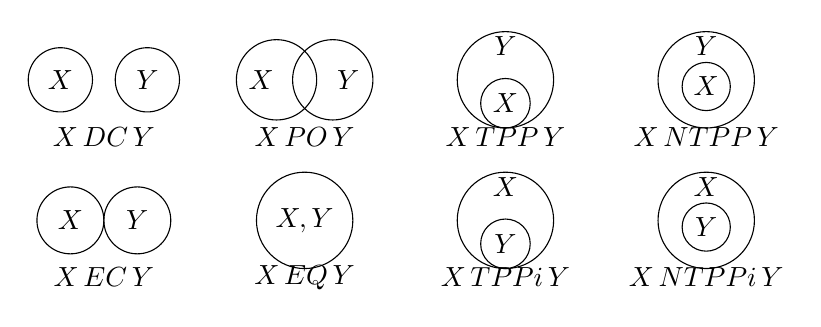
\begin{tikzpicture}[x=1cm,y=1cm,scale=.85]
\begin{scope}
\draw (-.65,.5) circle (.48);\draw (.65,.5) circle (.48);
\node at (-.65,.5) {$X$};\node at (.65,.5) {$Y$};
\node at (0,-.35) {$X\,DC\,Y$};\end{scope}
\begin{scope}[xshift=3cm]
\draw (-.42,.5) circle (.6);\draw (.42,.5) circle (.6);
\node at (-.65,.5) {$X$};\node at (.65,.5) {$Y$};
\node at (0,-.35) {$X\,PO\,Y$};\end{scope}
\begin{scope}[xshift=6cm]
\draw (0,.5) circle (.72);\draw (0,.15) circle (.37);
\node at (0,1) {$Y$};\node at (0,.15) {$X$};
\node at (0,-.35) {$X\,TPP\,Y$};\end{scope}
\begin{scope}[xshift=9cm]
\draw (0,.5) circle (.72);\draw (0,.4) circle (.36);
\node at (0,1) {$Y$};\node at (0,.4) {$X$};
\node at (0,-.35) {$X\,NTPP\,Y$};\end{scope}
\begin{scope}[yshift=-2.1cm]
\draw (-.5,.5) circle (.5);\draw (.5,.5) circle (.5);
\node at (-.5,.5) {$X$};\node at (.5,.5) {$Y$};
\node at (0,-.35) {$X\,EC\,Y$};\end{scope}
\begin{scope}[xshift=3cm,yshift=-2.1cm]
\draw (0,.5) circle (.72);\node at (0,.5) {$X,Y$};
\node at (0,-.35) {$X\,EQ\,Y$};\end{scope}
\begin{scope}[xshift=6cm,yshift=-2.1cm]
\draw (0,.5) circle (.72);\draw (0,.15) circle (.37);
\node at (0,1) {$X$};\node at (0,.15) {$Y$};
\node at (0,-.35) {$X\,TPPi\,Y$};\end{scope}
\begin{scope}[xshift=9cm,yshift=-2.1cm]
\draw (0,.5) circle (.72);\draw (0,.4) circle (.36);
\node at (0,1) {$X$};\node at (0,.4) {$Y$};
\node at (0,-.35) {$X\,NTPPi\,Y$};\end{scope}
\end{tikzpicture}
\caption{Native vector re-presentation of the eight ordinary region
configurations in Ragni's Figure~13.2.1. Circle radius and page position
are illustrative only. The inverse of \(NTPP\) is written \(NTPPi\),
repairing the source caption's transposed-letter spelling.}
\label{fig:p19-rat132-rcc}
\end{figure}

RCC-5 suppresses boundary distinctions: \(DC\) and \(EC\) merge
as discrete regions, \(TPP\) and \(NTPP\) merge as proper part,
and their inverses merge; partial overlap and equality remain. Thus the
five relations are discrete, partial overlap, proper part, inverse proper
part and equality. Whether countries share a border motivates keeping the
RCC-8 distinction. Neither system states which country is north of another.
Uncertain region descriptions again use disjunctions. The chapter mentions
the double-cross calculus, multidimensional interval extensions, robotics,
plan generation, sea navigation and language processing to illustrate
different formal/application domains; these named projects are not
interchangeable complete calculi or evidence that one cognitive account
explains every application.

\section{Six cognitive effects and the source's preferred arrangement}
\label{sec:p19-rat132-effects}

Ragni reviews the following effects, each requiring its original task and
comparison before a quantitative or population-level conclusion is drawn
\cite[sec.~3, pp.~728--729]{Ragni2021SpatialTemporal}.

\paragraph{Indeterminacy.} Descriptions compatible with several scenarios
are often harder than determinate ones in inference tasks. Mental-model
and mental-rule accounts both explain versions of the effect. It is not
a theorem that every multiple-model task is harder: producing \emph{any}
satisfying drawing provides more successful answers when more are allowed.
The primary experiment below makes this contrast concrete.

\paragraph{Relational complexity.} Higher-arity relations such as ternary
between, or information requiring decomposition into simpler relations,
can increase processing difficulty. Number of sentences and relational
arity are not the same measure. A claim about the cost of comparing four
objects is not automatically an effect of storing four independent premises.

\paragraph{Visual impedance.} Easily visualized descriptions can impede
relational inference relative to abstract descriptions. Ragni takes this as
support for an abstract-relational representation rather than a detailed
picture. Image construction followed by extracting relevant relations and
activation of additional declarative features are different proposed
mechanisms. The review does not settle which mechanism uniquely explains
every impedance finding, nor does it say all visual aids harm reasoning.

\paragraph{Continuity.} The source compares \(A<B,B<C,C<D\) in
that order with \(A<B,C<D,B<C\), where \(<\) here means
left-of. Both entail the same linear order; the discontinuous presentation
requires retaining two disconnected pieces before integrating them.
Content equivalence therefore does not imply equal processing demands.

\paragraph{Relevance.} An irrelevant or already-supplied conclusion premise
can make a task easier than one with equally many wholly relevant premises.
The proposed model stores what matters to the query. This is a contextual
claim about the compared tasks, not permission to discard a premise that
changes which countermodels are possible.

\paragraph{Preference.} The source's four car premises state Ferrari left
of Porsche, Beetle right of Porsche, Porsche left of Hummer and Hummer
left of Dodge. With one line and distinct positions they permit these
three orders:
\[
\begin{array}{cl}
1&\text{Ferrari Porsche Beetle Hummer Dodge}\\
2&\text{Ferrari Porsche Hummer Beetle Dodge}\\
3&\text{Ferrari Porsche Hummer Dodge Beetle}.
\end{array}
\]
The chapter calls the first the preferred model and describes higher/faster
acceptance of it than of the second, which in turn is favored over the
third. The question whether Beetle is \emph{necessarily} left of Dodge
exposes the cost of neglecting the third arrangement.

\begin{hbtheorem}{thm:p19-rat132-cars}{proved=annex:p19.rat132.cars}{All three orders, and the preferred-model error}
On one strict linear spatial order with all five cars at distinct positions,
the car premises have exactly the three displayed qualitative orders.
Porsche is necessarily left of Dodge. Beetle left of Dodge is possible
but not necessary; Beetle right of Dodge is also possible. In the graph
whose moves are swaps of adjacent cars preserving the premises, the
three orders form a path \(1\! -\!2\! -\!3\).
Model~3 is two such moves from model~1, not one.
\end{hbtheorem}

This graph is a declared discrete move system, not a theorem forbidding
every conceivable continuous motion in three-dimensional space. Allowing
tied positions adds configurations; allowing another axis changes what
left means. Nothing in the three-order proof measures how likely a person
is to construct one of those orders.

The source also reports that model insertion can be easier for large-scale
cardinal-direction problems than for small-scale left--right arrangements.
This domain comparison is not a consequence of the car-order theorem or
a guarantee for every navigation task. The source describes these effects as repeatedly reported and invokes
cross-cultural similarities and differences, small- and large-scale space,
topological tasks and some other domains. Those are review-level claims
whose individual populations, assignments, estimates and uncertainty are
not supplied in chapter~13.2. They must not be treated as one pooled
experiment, a universal effect size or proof of unrestricted transfer.

\section{PRISM: representation, construction, inspection and variation}
\label{sec:p19-rat132-prism}

Ragni contrasts coordinate-based models with discrete lists/grids,
visual-image architectures such as Casimir, and abstract or verbally
inspired relational accounts. The source's principal computational example
is PRISM, preferred inferences in reasoning with spatial mental models.
Its original presentation specifies five interacting components: input
triples \((X,r,Y)\) naming a located and reference object, abstract object
tokens, a two-dimensional spatial array, a movable focus and a control
process. Here \(X,Y\) name object tokens rather than the planar regions
of the RCC illustration. It presupposes an interpretation of spatial expressions; it does
not implement a natural-language understanding system
\cite[pp.~563--570]{RagniKnauff2013PRISM}.

Construction starts with an empty array. The first-mentioned token of the
first premise is inserted, then the second is placed in the relation's
direction. A subsequent one-new-token premise locates the already
represented reference, then inserts the new token. A two-new-token premise
creates another submodel. A connecting premise groups and integrates
submodels. These distinctions explain why continuous and discontinuous
premise sequences need different operations even when their final premise
sets agree.

If a desired cell is occupied, \emph{first free fit} (fff) proceeds farther
in the indicated direction to a free cell, preserving the placement of
existing tokens. \emph{First fit} (ff) instead relocates tokens to open the
nearest appropriate cell. For Porsche right of Ferrari followed by Beetle
left of Porsche, fff gives Beetle--Ferrari--Porsche while ff gives
Ferrari--Beetle--Porsche. Both obey the premises; the strategy, not the
semantics alone, chooses between them. An annotation records the constrained
token's relation to an anchor so that a later variation can preserve what
the premises actually asserted.

Inspection scans from the last focus position to identify a relation between
queried tokens. Variation starts from the preferred model, using small
changes constrained by annotations. A neighborhood graph organizes nearby
alternatives. Counting focus insertion, movement, refocusing and grouping
operations gives the proposed cognitive-complexity measure. The original
worked continuous/semicontinuous/discontinuous traces count 9, 10 and 12
operations, respectively. These are counts under specified program
conventions, not measured response-time components. Thus the specified
continuous trace has fewer operations than the semicontinuous trace,
which has fewer than the discontinuous trace. Equal operation costs are
an explicit original default
\cite[pp.~566--576,578,584]{RagniKnauff2013PRISM}.

A material qualification concerns the search policy. The 2021 chapter
describes constructing alternatives as counterexample search. The original
2013 PRISM distinguishes variation from systematic validation and expressly
does \emph{not} routinely search for counterexamples when a queried relation
already holds in the preferred model. Variation is particularly triggered
by an explicit all-model request or a relation absent from that model.
This asymmetry helps generate illusory necessity judgments. Correct
normative validation and the model's descriptive search policy must not be
conflated \cite[pp.~568--572,584]{RagniKnauff2013PRISM}.

Likewise, Ragni's resource-bounded interpretation is not an assertion that
the 2013 implementation contains every proposed resource limitation. Its
array capacity is not limited, information-decay is set to zero, and all
focus operations receive equal cost. It omits a belief/knowledge interaction
mechanism and a lexical semantics for fuzzy, intrinsic or viewpoint-dependent
prepositions; it is restricted to two horizontal dimensions, lacks diagonal
reasoning and disallows two tokens in one cell. The operational-parsimony
theory and these implementation defaults have different standing. Simulating
a response pattern shows that a proposed procedure can generate it, not
that the human brain must implement that exact procedure
\cite[pp.~582--585]{RagniKnauff2013PRISM}.

\section{Two primary spatial experiments}
\label{sec:p19-rat132-spatial-evidence}

The original PRISM paper provides experimental checks that are more specific
than the chapter's global preference statement. Its Experiment~1 used
20 Princeton students, nine female, mean age 23.4 years, as their own
controls. Two determinate, two indeterminate one-dimensional and two
indeterminate two-dimensional patterns were each presented twice: twelve
problems, randomized with fruit tokens randomly assigned. Premises were
self-paced, accumulated on screen, then disappeared before participants
drew an arrangement. Multiple drawings were permitted, but neither
requested nor announced as sometimes possible
\cite[pp.~578--579,581, Experiment~1]{RagniKnauff2013PRISM}.

In these reported tests, \(p\) denotes the source's tail-probability
value, not an interval or object token. Correct drawings were reported
for 83 percent of determinate and 92 percent
of indeterminate problems (\(p<.01\)). The authors explain the latter
advantage by the generation task's larger set of correct drawings; it does
not contradict a harder necessary-inference task. In indeterminate problems
the authors report a single drawing in 90 percent of problems; only two participants drew
more than one. Among correct indeterminate drawings, 78 percent followed
fff and 22 percent ff (\(p<.01\)). This conditional denominator is not
78 percent of all trials or all people. The report gives no confidence
intervals, participant-level response table or probability recruitment frame.

Experiment~2 used 25 Freiburg students, eleven female, mean age 23.9 years,
and 24 indeterminate four-premise fruit problems. Half the offered models
were consistent and half inconsistent; the article does not report results
for the inconsistent ones. Premises appeared sequentially, self-paced, each
replacing the previous premise. Participants then judged whether an offered
arrangement was a \emph{possible} model, not whether one relation was
necessary. The consistent alternatives were fff, mixed-strategy and ff
models. Correct acceptance was 92, 81 and 44 percent, respectively. Reported
time comparisons follow the same increasing difficulty order; the printed
numerals are ``3.797 ms'', ``4.359 ms'' and ``6.410 ms''. Their decimal/
thousands convention is not clarified in the report, so these are not
silently converted into calibrated stage durations. The printed trend
tests use Page's \(L\), here a trend-test statistic rather than the
light interval, with \(L=3.55,p<.001\) for error and
\(L=234.5,p<.01\) for response time. No uncertainty intervals or
individual response-time distributions are given
\cite[p.~580, Experiment~2]{RagniKnauff2013PRISM}.

The pattern is consistent with nearby alternatives being easier to recognize,
but acceptance and response time alone do not uniquely establish the exact
sequence of internal swaps. University samples, fruit descriptions, displayed
candidate arrangements, premise visibility and query wording bound the
claims. The 20- and 25-person studies are separate populations and designs;
their results cannot be combined as forty-five independent realizations of
one common task. In particular, accepting a possible arrangement is not
testing a necessary consequence.

\section{Durative temporal reasoning: a distinct primary task}
\label{sec:p19-rat132-temporal-evidence}

Kelly and Khemlani's account represents punctate events by one token when
duration is irrelevant, and durative events by start/end tokens. Its three
principles are iconic structure reflecting chronological order, an intuitive
initial construction versus deliberative revision, and a cost of maintaining
additional models. A discrete model need not depict every timepoint or
encode a ratio between seconds and decades. These are representational
proposals; Allen's thirteen relations were not designed as thirteen primitive
English expressions. ``Starts'' may require a sentence combining equal
beginnings with an earlier ending, and natural-language ``during'' may have
more than one interpretation \cite[pp.~1--3]{KellyKhemlani2019Durative}.

Their illustrative point-order description puts a meeting before a sale,
the sale after a conference, and the meeting before the conference:
meeting--conference--sale. Their durative illustration instead puts the
meeting during the sale and before the conference. The sale can end before
or after the conference; a single initial timeline does not settle this.
This is temporal indeterminacy, not rigid-object rotation.

\begin{hbtheorem}{thm:p19-rat132-durative}{proved=annex:p19.rat132.durative}{The actual alarm/fire/siren contrast}
Interpret during as strict interval containment \(d\), and before as
\(b\), for proper intervals. Alarm during fire and siren before alarm
are consistent both with a siren outside the fire and with a siren during
it. Adding fire during siren makes the premises inconsistent; adding siren
during fire instead makes them consistent. Thus rejecting the latter
description solely because it conflicts with the first chosen arrangement
is not a complete consistency check.
\end{hbtheorem}

The primary experiment recruited 50 native-English-speaking Mechanical Turk
participants for \$2 and a ten-percent chance of a \$10 bonus. Five were
excluded for inappropriate/excessive keypresses or irrelevant debriefing
responses, leaving 45 (21 female, mean age 35). All but six of the original
participants had at most one introductory logic course. It reports a
preregistered prediction and an OSF data locator; this treatment does not
claim to have independently rerun the dataset or audited the preregistration.

Each participant completed sixteen problems, four per cell of a fully
repeated \(2\times2\) design: initial one-model versus multiple-model
patterns, crossed with a consistent versus inconsistent third premise.
Each problem had three relations among three events, beginning with
\(X\) during \(Y\). Comparable-timescale everyday event triplets
avoided strongly punctate events and intended causal associations. Materials
were rotated across structures and order randomized. Participants revealed
premises with the spacebar while earlier premises remained visible, then
pressed f for consistent or j for inconsistent. A practice problem preceded
the task; four open debriefing questions followed it. These visibility and
response conditions differ from PRISM Experiment~2
\cite[pp.~3--4; Appendix]{KellyKhemlani2019Durative}.

Here \(z\) and Cliff's \(\delta\) denote the reported standardized
test statistic and effect-size measure. Reported accuracy was 78 versus
69 percent for one- versus multiple-model
patterns (Wilcoxon \(z=3.02,p=.003\), Cliff's \(\delta=.43\)).
The unadjusted consistency contrast was 72 versus 75 percent
(\(z=1.12,p=.27,\delta=.17\)); this is not equivalence evidence.
The interaction was \(z=4.03,p<.0001,\delta=.42\): consistent
multiple-model problems were particularly difficult, while inconsistent
problems showed little model-number difference. Figure~1's bars are
95-percent confidence intervals, without a printed table of their numerical
endpoints. No response-time result is reported; a theory's speed prediction
must not be relabeled an observed result.

The reported logistic mixed model included the two factors and interaction,
participant intercepts and slopes, and intercepts for items and relation
patterns. Here \(b\) denotes a fitted regression coefficient, not the
before relation. It found a one/multiple contrast
\(b=2.02,z=3.41,p=.0006\), an interaction
\(b=2.35,z=3.21,p=.0013\), and a consistency effect
\(b=1.82,z=4.34,p<.0001\) absent from the unadjusted comparison.
These coefficients belong to that fitted model, not nine-point accuracy
differences or odds ratios reported without a specified contrast coding.
The differing analyses and the unpredicted consistency effect remain visible
\cite[pp.~4--5, fig.~1]{KellyKhemlani2019Durative}.

The authors identify three limits: some participants reported pattern-based
strategies; errors do not reveal whether alternatives were never attempted
or attempted unsuccessfully; and the sixteen three-event structures give
only four problems per cell. A broader interpretation of during as overlap
changes some normative labels. It cannot make an already-consistent strict-
containment description inconsistent, but may make some labeled inconsistent
ones consistent. Accordingly, the particularly poor consistent-multiple
performance survives that particular semantic objection, without proving
that all labels, all ``while'' problems or a general temporal mechanism are
validated. The single experiment is neither a cross-cultural replication
nor an intervention showing that training transfers to navigation
\cite[pp.~5--6]{KellyKhemlani2019Durative}.

\section{Neural, content and rationality boundaries}
\label{sec:p19-rat132-limits}

Ragni's neural review separates frontal control/premise integration from
parietal representation and highlights superior parietal involvement.
It refers to the 47-fMRI-study Wertheim--Ragni meta-analysis, describing
frontal Brodmann areas~6 and~45 and parietal area~7. It also reports a
2016 TMS study: disruption of superior parietal processing reduced preferred-
model construction without a reported comparable reduction for alternatives,
and working-memory capacity moderated susceptibility. These remain the
chapter's review reports. Chapter~13.2 gives neither the TMS sample and
full stimulation/control protocol nor the effect estimates and uncertainty
needed to establish those original causal/localization claims here.
The cross-linked neural treatment in
\cref{sec:p19-rationality-1-4} distinguishes convergent evidence from
one-to-one mapping of a reasoning process to a brain region. Neither a
regional association nor a selective reported null proves a monolithic
storage module or complete independence of construction and variation
\cite[sec.~4, p.~729]{Ragni2021SpatialTemporal}.

Content, background beliefs and embodied response arrangements also matter
in the chapter's argument. A familiar silverware arrangement may guide
the initial model. Its SNARC discussion contrasts faster left-hand responses
to smaller numbers with faster right-hand responses to larger ones, then
reports a related spatial-relation/response-side effect. These are bounded
review illustrations, not a finding that all cultures, handedness groups
or every numerical and spatial task share a fixed left--right mental axis.
The source's conclusion that embodiment matters does not identify the
representational mechanism uniquely \cite[secs.~5--6]{Ragni2021SpatialTemporal}.

The source's blood-relatedness example makes the danger of indiscriminate
transitivity concrete: a father and daughter are blood-related, as are the
daughter and mother, but the parents need not be blood-related to one
another. The transitivity theorem for an ordered spatial axis cannot be
transferred to this symmetric but nontransitive relation. A linear mental
layout may explain an erroneous answer; it does not repair that answer's
logic. Likewise, RCC contact, interval overlap and ``is a relative of''
must not acquire transitivity just because before and northward order have it.

Ragni defends preferred-model parsimony as sensible under limited time,
working memory and computing resources, and suggests that finding an optimal
path or time plan may cost more than everyday purposes require. This is
a process-sensitive bounded-rationality argument. It does not alter the
formal distinction between possible and necessary, specify a universal
resource budget, supply an empirical utility function, or prove that every
observed error is optimal. When a wrong route, missed deadline or false
necessary inference has high consequences, the saved effort must be compared
with those losses and with available alternatives. Explaining a systematic
error and recommending the mechanism are different claims
\cite[secs.~6.3--7, pp.~731--732]{Ragni2021SpatialTemporal}.

For consultation, choose a relation benchmark matching the question.
Use one model to witness possibility; use a countermodel to refute necessity;
use a complete procedure or justified invariant to establish necessity or
inconsistency. Respect endpoint equality, boundary contact, query wording,
premise visibility and the declared frame. The car-order and durative
examples supply actual success/failure cases; a nonempty propagation fixed
point, a favored arrangement or an unqualified transitivity heuristic
supplies no general validity certificate.

\Cref{sec:p19-mental-rotation} instead studies congruence after a rigid
transformation, arbitrary feature bindings, response times and eye movements.
Its visual-transform evidence does not discharge relational-inference
claims. \Cref{sec:p12-rationality-13-1} treats external diagram syntax,
semantics and sound transformations; an Euler free ride valid in every
interpretation is not the extra left--right relation of one preferred
internal model. Both comparisons preserve the distinction between a
representation's normative meaning and its processing properties. The
empirical-record discipline of \cref{def:p19-evidence-record} applies
separately to the spatial and temporal studies. No missing original TMS,
cross-cultural, visual-impedance or response-side evidence record is filled
by borrowing the populations or estimates of the primary experiments above.

% ED26-BM-RAT2021-15-1 C01--C05: Markovits2021 developmental treatment.
\chapter{The development of basic human rationality}
\label{sec:p19-rationality-15-1}

Developmental evidence does not support identifying rationality with a single
score that inevitably increases with age. A child can draw an appropriate
inference without explaining its necessity; an adolescent can identify a
fallacy in a neutral argument yet overlook it in a favored argument; an adult
can understand validity but fail on a demanding inference. Markovits's 2021
chapter organizes these differences through explicit and implicit rationality,
and compares explanations based on reflection, social interaction, biological
specialization, cognitive capacity and semantic knowledge. Its conclusion is
an interaction account, not an agreed universal developmental timetable
\cite[pp.~779--787]{Markovits2021DevelopmentRationality}.

\begin{hbdefinition}{def:p19-r151-explicit-implicit}{Explicit and implicit rationality in the selected chapter}
\emph{Explicit rationality} concerns reasons offered for an inference, or
explicit assessments of why one inference is more adequate than another.
\emph{Implicit rationality} concerns the adequacy of judgments or inferences
actually produced, whether or not the participant gives an account of their
adequacy. \emph{Metalogical understanding} makes features such as inferential
validity and logical necessity objects of reflection. These are different
constructs, not three interchangeable names for an observed correct response.

The chapter mostly evaluates inference against standard logical norms,
because that is the orientation of much of the developmental work it reviews.
It also discusses practical, contextual and social adequacy. A task must
therefore specify its criterion: deductive necessity given stipulated premises
is not the same as empirical truth, a plausible causal expectation, or success
in a social exchange \cite[p.~779]{Markovits2021DevelopmentRationality}.
\end{hbdefinition}

\section{Reflection, argumentation and the use of competence}
\label{sec:p19-r151-explicit}

Moshman's account distinguishes making an inference from reasoning under an
understanding of its goals and standards. Reflection on particular inferences
can make their common structure explicit; increasingly general epistemic
understanding can continue into adulthood without a necessary endpoint.
The developmental claim concerns the construction and use of metalogical
concepts, not the first appearance of every valid inference. Correct modus
ponens is compatible with an inability to explain the difference between truth
and validity. Conversely, an explicit concept does not ensure its successful
application in every situation. Markovits identifies the relation between
developing explicit understanding and actual inference as an unresolved
empirical dependency. The adult confidence studies he cites do not provide a
longitudinal developmental test of that dependency
\cite[pp.~779--780]{Markovits2021DevelopmentRationality}.

Argumentation adds a social route: inferences and justifications are organized
to defend a position or challenge another. The social-constructivist account
suggests that encountering conflicting positions can prompt reflection on
relative inferential strength. The chapter reviews conservation interactions,
collaborative reasoning and Kuhn's argumentation interventions as evidence
relevant to this route. Those studies have different outcomes: a conservation
judgment, a selection-task answer, a dialogue strategy, and an individual essay
are not one measure of general rationality. A claim of improvement must name
which changed, under which interaction, and whether transfer was tested
\cite[pp.~780--781]{Markovits2021DevelopmentRationality}.
Markovits locates the contrast partly in the locus of development: individual
reflection on inferential structure versus socially produced confrontation of
positions. Both can advance explicit understanding without completely
determining subsequent judgments.

The argumentative account attributed to Mercier and Sperber gives a different
role to social interaction: argument production can serve persuasion and an
individual's position rather than impartial appraisal. Markovits contrasts
this with the expectation that confrontation necessarily leads toward better
explicit standards. His adolescent belief-bias example, attributed to
Klaczynski (2001), describes stronger detection of defects in relatively neutral
arguments than in arguments favoring emotionally held beliefs. It illustrates
context-sensitive deployment, not a demonstration that all adolescents lack
the relevant skill or that persuasion and truth are always opposed. These are
the chapter's theoretical and qualitative study comparisons; neither account
is established solely by the existence of a biased response
\cite[pp.~780--781]{Markovits2021DevelopmentRationality}.

% C05 continuation for ED26-BM-RAT2021-15-1. New reader material only.
% Root-owned placement: after the core's explicit-rationality/argumentation
% discussion. Existing core, prior evidence fragment and P11 record unchanged.
\subsection{Collaborative selection is not yet developmental transfer}
\label{sec:p19-r151-collaborative-interface}

Moshman and Geil's 1998 original experiment already has its full methodological
and numerical record in \cref{sec:p11-ri-individual-social}, with response-unit
conventions at \cref{def:p11-ri-collaborative-statistics}. It is the same
experiment cited in the developmental chapter, not a second independent
demonstration. Course-based undergraduates completed an abstract four-card
task individually or in consensus-oriented groups of five or six, with
written explanations. The original source gives 143 participants but compares
32 individual outputs with 20 group outputs. Its pooled 15/20 correct group
solutions and 3/32 correct individual solutions are not an age comparison
or 143 independent group trials
\cite[pp.~233--236]{MoshmanGeil1998CollaborativeReasoning}.

The developmental relevance lies in a possible mechanism: participants can
combine partial insights into a justified argument. In the two illustrated
groups, an argument for checking the odd-number card was combined with
an argument against checking the even-number card; neither group initially
contained a member choosing the complete correct pattern. Such construction
is different from counting votes or copying an initially complete answer.
Those illustrations were purposively selected from three all-initially-
incorrect groups; the third videotape was lost. The paper supplies no
formal process-coding reliability or isolated mediation estimate
\cite[pp.~237--245]{MoshmanGeil1998CollaborativeReasoning}.

The original discussion nevertheless does not establish a general childhood
developmental effect. Participant ages and a child cohort are not supplied.
Responses are immediate, on the same task, following discussion; no delayed
or novel-task test demonstrates lasting individual transfer. Group discussions
took approximately two-and-a-half times the individual solving time, without
a time-yoked control. Eliminating simple adoption of the initial majority
answer does not eliminate every influence of confidence, status or later
consensus. These limits accompany the existing original-study record rather
than being replaced by a generic claim that collaboration improves rationality.

At p.~246 the authors explicitly decline to claim durable, generalizable
competence change from this brief interaction. Their prediction that groups
of children younger than eleven or twelve might fare no better than individual
children, if the task requires a particular metalogical competence, is a
conditional prediction, not an observed child result. Repeated dialogic
learning is a proposed developmental route. The two adolescent interventions
below test related but different outcomes; they cannot retroactively turn
the undergraduate selection experiment into childhood longitudinal evidence
\cite[pp.~242--246]{MoshmanGeil1998CollaborativeReasoning}.

\subsection{Kuhn and Udell's 2003 intervention: discourse and its individual product}
\label{sec:p19-r151-kuhn-udell}

Kuhn and Udell distinguish an individual argument supporting a claim from
argumentative discourse responding to an interlocutor. Their intervention
targets a shift from articulating one's own position to engaging the
opponent's reasons, including critique and rebuttal. The assessment criterion
is a source-defined discourse/argument rubric, not an answer key identifying
the ethically correct position on capital punishment. More coded
counterarguments do not by themselves prove greater logical validity
\cite[pp.~1245--1248]{KuhnUdell2003Development}.

The analyzed sample comprised 34 eighth graders from two low-performing
New York City public middle schools. The article describes its target group
as academically at-risk thirteen-to-fourteen-year-olds but gives no individual
age distribution. It reports 14 Hispanic, 19 African-American and one
Ethiopian participant; 11 male and 23 female. These are the reported
sampling descriptors, not diagnoses or population-wide competence judgments.
There were 21 completers in the experimental condition and 13 in comparison.
Five additional starters, three experimental and two comparison, did not
complete because of chronic absence or suspension. Thus 39 started and
34 completed; outcome-specific samples are smaller in some analyses.

The authors report random assignment to conditions without specifying its
algorithm. Teams were then formed from pro/con opinions. The experimental
teams were represented at both schools; the comparison teams were at one
school. Team sizes were four to eight, with typical attendance three to
six. Recruitment/response rates, consent details and native-language
eligibility are not reported. English task formulations are supplied.
School, team and discussion-partner dependence remain relevant to inference
\cite[pp.~1247--1250]{KuhnUdell2003Development}.

The full condition received sixteen sessions scheduled twice weekly for
ninety minutes. Interruptions extended the nominal eight-week schedule to
approximately twelve weeks. Both conditions shared the first seven sessions,
developing reasons, elaborating them, using evidence, evaluating reasons,
and assembling an argument. Comparison activity ended after this phase;
it did not receive nine matched-duration alternative sessions. The full
condition continued with opposing-side reasons, counterarguments, rebuttals,
mixed evidence, practice dialogues and a final debate. The difference is
therefore a scaffolded package with more exposure, not a dialogue-only
manipulation at equal dose.
Comparison pupils also engaged in same-side team activity; this was not
an individual-only or no-collaboration control.

Adult coaches supported the activities. Participants made reason cards,
considered how an opponent would react, attached evidence and rebuttal cards,
and revised or dropped reasons. Some evidence articles were initially
presented without later opposing-perspective paragraphs, which were restored
in the mixed-evidence phase. Coaching, external representation, evidence
access, competitive goals and peer response are substantive ingredients.
The final debate used rotating speakers and short team consultations.
None was independently varied to identify one unique active component
\cite[pp.~1250--1251]{KuhnUdell2003Development}.

Individual assessments before and after activity elicited the participant's
opinion and supporting reasons, then all reasons that someone might offer
on either side. Unique reasons indexed topic-specific knowledge. Product
quality used a hierarchy: unsupported or weakly justificatory reasons,
conditions/administrative objections, reasons addressing the institution's
functions, and functional reasons comparing it with alternatives. An
argument could also become two-sided by including reasons on both sides.
That is the authors' evaluative rubric; an administrative injustice does
not become morally unimportant simply because the rubric places it below
a comparative functional reason. Seventy percent of product responses were
double coded: 81 percent agreement, Cohen \(\kappa=.67\).

Discourse assessments paired students with opposing opinions, usually with
the same partner at pre/post assessment, for videotaped ten-minute dialogues.
Utterances were segmented and coded by their relation to the opponent's
preceding move. \emph{Counter-A} introduced an alternative argument;
\emph{Counter-C} criticized that move. \emph{Clarify} elaborated one's
own position; \emph{Add} elaborated conversationally without advancing
the argumentative goal. A rebuttal sequence was a counter followed directly
by Counter-C. The full source appendix distinguishes further questions,
agreement, interpretation and other functions. Off-topic and meta-dialogue
utterances were excluded from the proportion analyses. Training used
15 percent of dialogues, and a fourth rater recoded 25 percent of the
remaining coded material: 90 percent agreement, \(\kappa=.72\).
Coding reliability concerns the specified categories, not truth of the
participants' substantive claims
\cite[pp.~1248--1249,1252--1253,1259--1260]{KuhnUdell2003Development}.

For the statistics in these records, \(F\) is a reported analysis-of-variance
statistic, \(t\) a reported t-test statistic and \(p\) a statistical p-value.
One experimental dyad's recording was lost, leaving 32 participants for
discourse analysis, nineteen experimental and thirteen comparison. Mean
utterance counts per participant/dialogue changed from 7.23, SD~5.06,
to 29.58, SD~17.56, in the full condition, versus 7.15, SD~4.25,
to 11.11, SD~9.83, in comparison. These are within-dialogue utterances,
not independent participant recruitments. To separate composition from
volume, the authors analyzed utterance proportions with an arcsin
transformation and pretest covariates.

The overall group effect was \(F(5,25)=6.0,p=.001\). Counter-C
proportions rose from 5.3 to 30.6 percent in the full condition and
11.4 to 21.4 percent in comparison; its adjusted group test was
\(F(1,29)=4.21,p=.049\). Counter-A changed from 7.6 to 13.6
versus 5.3 to 1.2 percent, \(F(1,29)=21.07,p=.001\).
Clarify declined from 37.2 to 18.5 versus 44.3 to 32.4 percent.
Simple disagreement did not meet .05 in its group test, \(p=.08\).
The source's effects are therefore not uniform across discourse categories
\cite[p.~1252, tables~3--4]{KuhnUdell2003Development}.

At least one Counter-C occurred for all nineteen experimental discourse
participants at posttest, versus ten of thirteen comparison participants;
initial counts were eight and five. Rebuttal-sequence means rose from .16,
SD~.50, to 3.79, SD~1.75, in the full condition, versus .23,
SD~.44, to .46, SD~.66, in comparison. The time/condition interaction
was \(F(1,30)=32.37,p<.001\). The paper prints no confidence intervals
for these contrasts and reports no dyad/team/school-adjusted outcome model.
The authors also stress that advanced strategies remained uncommon:
clarification requests and more complex sequences did not show a broad
uniform advance. Observed Counter-C usage is not mastery of every
argumentative skill
\cite[pp.~1253,1256--1257, table~6]{KuhnUdell2003Development}.

Individual-product quality used all 34 completers: positive change was
reported for 15/21 full-condition participants and 5/13 comparison
participants. The article describes that between-condition difference as
not reaching statistical significance. Eight of the fifteen experimental
improvements included a shift to two-sided argument. The knowledge-of-reasons
analysis instead omitted one experimental participant with a missing
all-reasons response. Per-assessment reason counts rose from 3.30 to 4.45
in that group and 2.31 to 2.54 in comparison, but the between-group gain
difference was not significant. Distinct reasons pooled across the two
assessments averaged 6.70 versus 4.38, with \(t(31)=3.23,p=.003\).
That pooled repertoire statistic is not the posttest gain or a new sample
\cite[pp.~1254--1255, table~7]{KuhnUdell2003Development}.

The authors themselves retain the possibility that extending Phase~I
could improve the comparison group because its total exposure was shorter.
This limits a claim that interaction with an opposing side alone caused
the difference. The outcomes concern one practiced topic and its pre/post
dialogue/product tasks. No delayed novel-topic transfer test is reported
in this experiment; transfers cited in its discussion belong to other
studies. The experiment supports changes under the implemented package,
with attrition, small samples and dependence retained, not a universal
age transition or a demonstration that every debate improves rationality
\cite[pp.~1256--1258]{KuhnUdell2003Development}.

\subsection{Kuhn and Crowell's 2011 study: extended practice and novel essays}
\label{sec:p19-r151-kuhn-crowell}

The 2011 intervention tests a different transfer: from sustained dialogic
activity to individually written essays on assessment topics not taught in
that activity. Entering sixth graders were eleven or twelve and attended
one academically challenging urban public middle school in the northeastern
United States. The neighborhood was ethnically diverse and low-to-middle
income; the article reports 80 percent Hispanic or African-American and
60 percent free/reduced-lunch eligibility. Individual age ranges beyond
the entry description, native-language eligibility and a probability
recruitment frame are not supplied.

The school formed three classes of thirty to thirty-two students matched
on gender, ethnicity and standardized scores. Two classes were randomly
selected for intervention and one for comparison. This is random assignment
at the level of only three classes, not independent randomization of
each student's curriculum. Table~\ref{tab:p19-r151-kuhn-crowell-samples}
keeps the overlapping and distinct outcome datasets separate
\cite[pp.~546--547]{KuhnCrowell2011Dialogic}.

\begin{table}[htbp]
\centering\small
\begin{tabularx}{\textwidth}{@{}Xrr@{}}
\hline
Dataset & Intervention & Comparison\\
\hline
Main longitudinal sample & 48 & 23\\
Expanded main Year~3 posttest sample & 60 & 28\\
External Year~3 comparison school & --- & 50\\
Following-entry replication & 37 & 21\\
\hline
\end{tabularx}
\caption{Student counts for distinct outcome samples in Kuhn--Crowell 2011. The first two
rows overlap and must not be added as independent recruited populations;
the external group was matched rather than randomly assigned.}
\label{tab:p19-r151-kuhn-crowell-samples}
\end{table}

In the longitudinal sample there were 27 girls/21 boys in intervention and
11 girls/12 boys in comparison. Most supplied at least three of four
assessments; one comparison student supplied only initial/final assessments.
Three missed the final assessment and seven missed one interim assessment.
The article does not specify an outcome-level missing-data/imputation
procedure that reproduces all printed inferential denominators. The
expanded posttest samples included pupils absent initially or arriving
later, with sex counts 31/29 and 13/15. The external fifty eighth graders
came from another city school matched on scores, lunch eligibility and
ethnic composition, not from the intervention's randomization.

Both curricula met twice weekly for fifty-minute philosophy classes.
The intervention spent about thirteen sessions per topic, four topics
per year, across three years. Same-side preparation generated and ranked
reasons. Partners then conducted electronic dialogues with six opposing
pairs, preserving chat transcripts for reflection. Group preparations,
a rotating-speaker debate, argument-map debriefing and a final essay
completed a topic cycle. Evidence materials were added from the final
topic of Year~1; students increasingly generated questions themselves,
with coaches supplying concise answers. Reflection changed form in
Year~3, and topics became three-sided. Note~2 records differences
between the two classes' Year~1 time allocation. This is a multicomponent,
changing curriculum rather than one constant dialogue-dose treatment.

Comparison students received teacher-led whole-class discussion, some
activities such as dramatization and more frequent essays: fourteen per
year versus four in intervention. Thus the control was educationally
active and had more writing practice, while coaching, peer structure,
reflection and evidence access differed. It does not isolate the causal
contribution of electronic rather than spoken dialogue or any single
ingredient
\cite[pp.~547--548,552, note~2]{KuhnCrowell2011Dialogic}.

Teacher-pay essays were assessed initially and after each of three years.
A separate assisted-dying essay appeared only at the Year~3 endpoint.
These were assessment subjects, not the curriculum's deeply studied
topics; neither political nor medical position was the answer key.
At Year~3, essays received twenty minutes and follow-up questions ten
minutes, with the teacher-pay assessment first on a different day.
The follow-up asked which unanswered questions would help the argument;
those assessment questions were not answered. More questions therefore
measure proposed evidence seeking, not actual verified information use.

The scoring categories preserve the source's distinctions. An own-side
argument offers advantages of the favored position. A \emph{dual perspective}
also attacks the opposing option, so all considerations can still favor
the same conclusion. An \emph{integrative perspective} acknowledges a
disadvantage of the favored position or advantage of its opponent, requiring
considerations leading in opposite directions to be addressed. This is
not identical to the 2003 paper's one-/two-sided argument coding.
Idea-unit coding was blind to condition and time; a random third of
essays was double coded. Agreement was 88 percent, \(\kappa=.76\),
for teacher pay and 93 percent, \(\kappa=.91\), for assisted dying.
Reliability of classification does not itself validate every factual
premise or normative recommendation within an essay
\cite[pp.~546,548--550, table~1]{KuhnCrowell2011Dialogic}.

For teacher-pay dual-perspective counts, the reported condition/time
interaction was \(F(3,67)=6.11,p<.001,\eta_p^2=.216\).
At Year~3, the percentages producing at least one dual-perspective
argument were 79 versus 29; integrative arguments appeared in 30 versus
zero percent, having been absent at earlier main-study assessments.
Both groups' essays became longer. Year~3 total argument means were
3.96 versus 2.61; the source also reports dual-perspective shares .49
versus .24 after accounting for overall production. Figure~1 error bars
are standard errors, not 95 percent confidence intervals.

On the new assisted-dying topic, dual-perspective argument counts averaged
1.17 versus .36, \(t(86)=3.85,p<.001\). Percentages supplying at
least one dual-perspective argument were 73, 29 and 24 for intervention,
internal comparison and external comparison; integrative percentages were
30, 18 and eight. These are different endpoints with different samples,
not universal success percentages. Proposed question counts averaged
4.18 versus .33 for teacher pay and 3.26 versus 1.64 for assisted dying,
with .92 in the external comparison. Counts and general-versus-case-specific
question coding support a limited evidence-seeking interpretation; the
article does not establish the future truth or usefulness of every question
\cite[pp.~549--551, tables~2--5]{KuhnCrowell2011Dialogic}.

The next incoming cohort provided a within-school replication through
Year~2, not an independent multi-population replication. After classroom
reassignment for behavior-management reasons, all students switching
conditions were excluded; note~4 does not give that exclusion count.
The retained sample was 37 intervention and 21 comparison students,
with comparison assessments available only at Year~2. Two intervention
responses were missing initially and two at Year~1. At Year~2,
dual-perspective count means were 1.05 versus .43,
\(t(56)=2.81,p=.007\), and integrative arguments appeared in 14
versus zero percent. Proposed question means were 1.48 versus .90,
but their difference was not significant, \(p=.148\). Replication
therefore does not mean every main-study outcome repeated at the same
strength or timing
\cite[pp.~550--552, table~6, note~4]{KuhnCrowell2011Dialogic}.

The paper supplies no interval estimates for these principal contrasts
and no reported class-cluster-adjusted model. Treating every pupil as
an independently randomized intervention unit would overstate the
randomization evidence. Attrition, changing membership, excluded
class-switchers, differences in adult facilitation and a restricted
school setting qualify causal and generalization claims. Nevertheless,
novel-topic individual essays provide an actual transfer outcome absent
from the undergraduate selection study and the same-topic 2003 experiment.
They do not establish transfer to abstract deduction, measured working-memory
capacity, an explicit concept of logical validity, all populations or
long-term performance after the curriculum ends.

\subsection{What these comparisons leave distinct}
\label{sec:p19-r151-social-capacity-boundary}

A complete selection under a stipulated conditional rule, a partner-responsive
counterargument, a higher-rated individual argument and an integrative essay
are different achievements. The first permits an exact truth-preservation
benchmark; the others use declared task-specific functional or evaluative
rubrics. The studies supply evidence at their measured times and scopes,
not one shared rationality score. The capacity and metalogical accounts in
this chapter additionally concern resource limits and explicit understanding.
These social-intervention outcomes do not directly measure either construct
or isolate capacity growth as their causal mechanism. A developmental
comparison must preserve what was practiced, what was tested, who was
sampled and whether a new topic or later occasion was actually observed.



\subsection{An original validity study: three tasks, three cohorts}
\label{sec:p19-r151-validity-record}

Moshman and Franks's 1986 paper investigated whether students distinguish the
necessary premise--conclusion relation from the empirical truth of its terms.
Experiment~1 recruited volunteers from Lincoln, Nebraska public schools:
20 fourth graders, ages 9 years to 10 years 6 months, mean 9 years 8 months,
and 20 seventh graders, ages 12 years to 14 years 3 months, mean 13 years.
The 41 University of Nebraska--Lincoln undergraduates came from a course
required of education majors; ages 18--37, mean 21.3 years. Undergraduates
reporting a logic course were not included; the count excluded is not given.
These are educational convenience samples, not representative age populations
\cite[pp.~153--156]{MoshmanFranks1986Validity}.

Seven arguments varied premise truth, conclusion truth and validity. Most used
transitive relations; a disjunctive inference prevented identification of all
valid items by identical form. Participants sorted argument trios and the whole
set and ranked the arguments. Children were individually interviewed with
movable cards, reading checks, follow-up questions and suggested sortings;
college students completed written booklets in small groups. That accommodation
reduces some expression demands but also makes the age comparison a comparison
of different administration modes. Validity coding required an explanation
distinguishing necessary consequence from truth, content or mere form; ranking
the three valid arguments above the others needed no verbal explanation.
Second coding of 50 written responses gave 82 percent category agreement and
98 percent agreement on the validity distinction.

The proportions using validity at least once were 0, 45 and 85 percent in the
fourth-grade, seventh-grade and undergraduate cohorts. The paper reports
\(\chi^2(2,N=81)=40.4,p<.001\). Zero successes among these 20 fourth
graders is an observation under the scoring and procedure, not proof that no
child of that age can possess a concept of validity. Among seventh graders,
individual responses ranged from fourth-grade-like to adult-like performance
\cite[pp.~156--158]{MoshmanFranks1986Validity}.

Experiment~2 used new volunteers: 18 fourth graders, ages 9 years 1 month to
11 years 4 months, mean 9 years 9 months; 18 seventh graders, ages 12 years
7 months to 13 years 11 months, mean 13 years; and 20 undergraduates, ages
19--23, mean 20.9. Recruitment used the same school and education-course
settings. Definitions, contrasting examples and explicit instructions preceded
40 validity judgments using five simple argument types with true, false or
neutral content. A separate ten-item control asked participants to choose the
better conclusion, rather than judge the validity of an entire argument.
The stringent criterion, at least 90 percent correct over 40 judgments, was
met by 11, 67 and 80 percent, respectively; a 70 percent criterion was met by
56, 89 and 100 percent. The control means were 9.6, 9.7 and 10.0 out of ten,
and nobody scored below eight. On the twelve critical items where truth and
validity conflicted, 11, 61 and 75 percent met the paper's above-chance validity
criterion of eleven or twelve correct
\cite[pp.~158--161]{MoshmanFranks1986Validity}.

Experiment~3 again used new volunteers: 20 fourth graders, mean 9 years
7 months, range 9 years to 10 years 5 months; 20 seventh graders, mean
13 years, range 12 years 5 months to 13 years 5 months; and 20 undergraduates,
mean 22 years, range 19--43. Within each age group, half were randomly assigned
an initial explanation of validity. All individually sorted the same forty
arguments with trial-by-trial correctness feedback and access to earlier cards.
Its success criterion was 90 percent correct over all forty, the last twenty,
\emph{or} the last ten judgments. That more permissive disjunctive rule is not
the identical measure used in Experiment~2. Success proportions were 10, 75
and 90 percent; \(\chi^2(2,N=60)=30.6,p<.001\). The paper does not report
confidence intervals for these proportions
\cite[pp.~161--164]{MoshmanFranks1986Validity}.

The authors favor a deficit in explicit validity understanding for most of
their fourth graders and a spontaneous-application limitation for many seventh
graders. They explicitly state that absent competence cannot be conclusively
proved and that new conditions might reveal it. Their evidence concerns several
cross-sectional cohorts, not an observed transition in each child between ages
ten and twelve. The strong control-task performance is decisive for keeping
ordinary inference separate from explicit validity classification. Nonsignificant
seventh-grade--college comparisons in the prompted tasks do not prove equal
population competence. The paper's internal contrasts test alternative task
explanations; they are not independent cross-cultural replications.

\section{Abstraction and biological proposals}
\label{sec:p19-r151-biological}

The chapter's Piagetian reconstruction links assimilation and accommodation
with reflective abstraction: common structure in lower-level activity becomes
available for more abstract operations. Its three broad levels are sensorimotor
action/perception schemas, concrete operations tied to objects, and formal
operations manipulating more general concepts. ``Locally rational'' means
coherence relative to the structures available at a level, not global conformity
to every logical norm. Markovits gives two opposing empirical pressures on a
simple stage interpretation: early successful deductions reported by Hawkins
and colleagues, and persistent adult errors. Overton and Ricco's
competence--performance distinction responds to the latter by separating
available logical capacity from conditions governing its use. The chapter
cites age-related instruction effects, but those effects do not independently
identify an unobserved competence structure
\cite[pp.~781--782]{Markovits2021DevelopmentRationality}.

Braine's natural-logic account proposes syntactic inference schemas, with a
biological argument that some rapid reliable inferences could serve survival.
Its interpretational component handles variability associated with pragmatics
and knowledge. This is neither a claim that every utterance is already in
formal notation nor a theorem that evolution installed a complete calculus.
Compare the full architecture of representation, schemas, control and pragmatic
integration in \cref{sec:p19-rationality-3-2}.

A different biological proposal attributes successful social-contract checking
to specialized cheater detection. The abstract selection task has four visible
cases: antecedent, nonantecedent, consequent and nonconsequent. For a stipulated
exceptionless conditional, the antecedent case can conceal a violation on its
reverse, and the nonconsequent case can conceal an antecedent. The remaining
two cases cannot conceal that particular violation. Thus checking a vowel--even
rule requires checking the vowel and odd-number cases. The chapter contrasts
poor abstract performance with improved performance under certain permission
or exchange rules and cites Cummins and Girotto and colleagues for children's
deontic versions. Agreement with the formal answer in that context does not
demonstrate domain-general logical competence or uniquely distinguish an evolved
module from learned pragmatic schemas. The drinking-age illustration is a
stipulated historical task rule, not a statement of current law
\cite[pp.~782--783]{Markovits2021DevelopmentRationality}.

Attachment supplies a further, explicitly different illustration of contextual
inference: expectations formed through interaction can organize later
interpretation of important others' behavior. Markovits connects Bowlby's
behavioral system, internal working models and adult romantic-attachment
research. These proposed social schemas do not establish truth-preserving
deduction; nor does a behavioral classification establish a particular caregiver
cause, a child's fixed future relationships, or an individual diagnosis.
The chapter's simplified caregiver examples must not be read as deterministic
causal laws or parenting advice. They illustrate experience-sensitive expectations,
not a measured developmental age trajectory
\cite[pp.~783--784]{Markovits2021DevelopmentRationality}.

\section{Conditional tasks and the capacity--content contrast}
\label{sec:p19-r151-conditionals}

\begin{hbconvention}{def:p19-r151-conditional-benchmark}{Necessity, invitation and uncertainty}
For the schematic discussion, \(P\) and \(Q\) are antecedent and consequent
propositions; \(A\) names an alternative antecedent. In an exceptionless
deductive reading of ``if \(P\), then \(Q\)'', asserting \(P\) supports
\(Q\) (MP), and denying \(Q\) supports denial of \(P\) (MT).
Asserting \(Q\) does not establish \(P\) (AC), and denying \(P\)
does not establish denial of \(Q\) (DA). A case with \(P\) false and
\(Q\) true is consistent with the conditional and defeats both invited
conclusions. Rejecting \emph{necessity} is not asserting that the invited
conclusion is false. A probabilistic or defeasible causal reading changes
the benchmark and must be declared separately.
\end{hbconvention}

Barrouillet's developmental mental-model explanation, as reconstructed by the
chapter, emphasizes the number of models working memory can maintain. The
initial represented case has both terms true. A second case with both false
gives the two possibilities of a biconditional; the additional case with a false
antecedent and true consequent supplies the full conditional possibilities.
Searching only the initial case favors MP and AC; the biconditional set favors
all four conclusions; the three-case set supports MP/MT but defeats AC/DA.
These are predictions of an assumed representation/search procedure, not
observed mental objects uniquely recovered from a response pattern. The
account also permits pragmatic interpretations that are appropriate to a
context without matching the intended formal benchmark; its strongest
capacity-based sequence must be distinguished from that qualification.

In the truth-table task, a participant classifies the four antecedent/consequent
combinations as making a rule true, false, or neither. This differs from
deciding whether an inference is necessary. Markovits reports a progression
from predominantly conjunctive judgments through biconditional judgments to
conditional judgments, associated with working-memory measures in selected
studies. The approximate ages he reports---eight or nine, eleven or twelve,
and mid-adolescence---describe those tasks and theoretical interpretations.
They do not license a universal calendar independent of language, content,
response categories or sampling. The chapter expressly cites the 2016
content-sensitive counterevidence
\cite[pp.~784--785]{Markovits2021DevelopmentRationality}.

\subsection{The original 2016 within-pupil comparison}
\label{sec:p19-r151-2016-record}

Markovits, Brisson and de Chantal tested 77 native French-speaking pupils
from an elementary school in the Montreal region: 35 in grade three,
20 girls and 15 boys, mean age 9 years 2 months; 42 in grade six,
21 girls and 21 boys, mean age 12 years 1 month. Entire classes received
booklets and common instructions. Each pupil evaluated two arbitrary
conditionals and two imaginary category--property conditionals; two booklet
versions reversed their order. Specific cases represented each of the four
antecedent/consequent combinations, with order varied. The paper does not
specify a probability recruitment frame, response rate, or interval estimates
for its pattern percentages
\cite[pp.~1908--1910]{MarkovitsBrissonDeChantal2016Conditionals}.

Arbitrary rules associated colors or clothing without an explicit relational
structure. The imaginary rules concerned category membership and properties
on an unfamiliar planet. The latter remove familiar factual knowledge while
retaining an interpretable category--property relation. This is not simply
``familiar versus unfamiliar words'': the rule types also differ in relational
structure and narrative framing. Responses were true, false or one-cannot-know.
A \emph{defective conditional} pattern marked the both-true case true, the
true-antecedent/false-consequent case false, and both false-antecedent cases
irrelevant. That pattern is not a complete material-conditional truth table,
which assigns true to its false-antecedent cases.

For grades three and six, respectively, defective-conditional pattern
percentages were 25.7 and 26.2 with imaginary rules versus 8.6 and 7.1 with
arbitrary rules. Conjunctive pattern percentages were 11.4 and 25.0 versus
22.6 and 39.3. Each pupil contributed two rule patterns per type; the reported
chi-square comparisons, \(\chi^2(1,N=70)=7.24,p<.01\) and
\(\chi^2(1,N=84)=8.85,p<.01\), therefore do not describe 70 and 84
independently recruited children. A within-subjects analysis of false responses
on the two false-antecedent combinations reported means 2.39 for arbitrary
and 1.71 for imaginary rules, with \(F(1,73)=14.08,p<.001\) for rule
type. Its degrees of freedom, and those in the separate basic-combination
analysis, do not provide a reported exclusion account; none is invented here
\cite[pp.~1910--1911, tables~1--2]{MarkovitsBrissonDeChantal2016Conditionals}.

The authors argue against a capacity-only explanation that preadolescents
cannot produce a more complex interpretation. They examine pragmatic-heuristic
and systematic-misinterpretation alternatives. Their contrast shows that a
uniform conjunctive limitation does not describe all these responses. It does
not directly measure working-memory capacity, prove that working memory never
matters, or establish identical comprehension in all children. High proportions
of incompatible and other patterns remain. The arbitrary-rule results partly
reproduce the earlier pattern, while the structured rules challenge its
unqualified generalization. This is a content-bound conceptual comparison,
not a longitudinal study or an independent multilingual replication
\cite[pp.~1911--1912]{MarkovitsBrissonDeChantal2016Conditionals}.

\section{Semantic retrieval, redescription and divergent thinking}
\label{sec:p19-r151-semantic}

Semantic redescription theory gives a different weight to knowledge. Premise
interpretation cues information in semantic memory, which can contribute
additional models. An alternative cause---another hard object breaking a
window---supports uncertainty about whether a rock caused an observed break.
A disabler---a resistant window---instead challenges the applicability of
the assumed causal rule. Retrieval is not necessarily restricted to the
information useful for the current inference: accessing alternatives can also
activate disablers. Thus improving search can lower acceptance of AC/DA yet
also lower acceptance of MP/MT. In a stipulated deductive task, inhibiting
premise-inconsistent information is appropriate to its benchmark; in an
empirical causal task, reconsidering the rule may be appropriate. The resulting
response cannot be evaluated without that task distinction
\cite[pp.~785--786]{Markovits2021DevelopmentRationality}; compare
\cref{sec:p19-rationality-5-4}.

The chapter distinguishes category--property, ordinary causal,
contrary-to-fact causal, and abstract conditionals. Its example relations are
dogs and legs, rocks and breaking windows, feathers and breaking windows,
and the uninterpreted terms XY and blrp. These vary the available meaningful
relation, not merely sentence length. Category knowledge can
supply an alternative animal with the named property; ordinary causal memory
can supply a different cause. Contrary-to-fact and uninterpretable abstract
rules require construction beyond that stored relation. Its reported pattern
places success with some category premises as early as seven or eight,
ordinary causal success later, contrary-to-fact success chiefly in later
adolescence, and consistently abstract success as difficult even for educated
adults. These are qualified summaries of selected studies, not required
success ages for each child. The theory proposes increasingly abstract
redescription of alternatives, rather than maturation alone. Markovits also
reports selective benefits of generating alternatives at a higher abstraction
level and interference from initially reasoning with abstract premises.
Those claims concern specified content and sequence, not a general instruction
that every additional example improves every reasoning task
\cite[pp.~785--786]{Markovits2021DevelopmentRationality}.

The divergent-thinking extension concerns generating possibilities beyond the
strong associations suggested by a premise. More ideas, more different
categories of ideas, and more original ideas are different measures. None is
identical to logical validity or to creativity in every domain. The chapter's
preschool example contrasts accepting a category inference with withholding
certainty about its converse, and discusses a preceding possibility-generation
exercise. The direct original records below delimit that claim.

\subsection{The original 2017 preschool records}
\label{sec:p19-r151-2017-record}

De Chantal and Markovits's Study~1 recruited 32 native French-speaking
children from a Montreal-region day-care center, 21 boys and 11 girls,
ages 41--64 months, mean 53.5 months. Parents consented. Individually
administered sessions in a quiet room lasted about fifteen minutes. Each child
completed idea generation, a dimensional-change card sort (DCCS), and reasoning,
with the first two tasks in one of two orders and reasoning always last.
Generation asked for ways of making noise, giving gifts and getting dirty,
with two examples for each prompt and no time limit. Flexibility was the mean
number of distinct response categories; fluency was mean number of responses.
Two category coders gave weighted kappa .798. The three-phase DCCS scored
threshold success in sorting by color, switching to shape, and switching under
a border rule. Although nominally zero to three, observed scores were only
one or two: all succeeded in phase one, none in phase three
\cite[pp.~210--214]{DeChantalMarkovits2017Alternatives}.

The reasoning task used three familiar universal category--property premises,
with AC followed by MP and requests for justifications. A point required both
accepting the necessary MP conclusion and withholding the AC conclusion for
the same premise; the total ranged from zero to three. Mean total was .81,
SD .90, equivalent to 27 percent of premise pairs, \emph{not} 27 percent
of children passing a universal competence criterion. Mean MP and AC scores
were 2.91, SD .39, and .91, SD .89, respectively. The published correlations
with total reasoning were .48 for flexibility, .37 for fluency and -.06 for
DCCS. Controlling fluency, the flexibility correlation was
\(r(29)=.353,p=.05\). These are small-sample associations, not intervention
effects; the restricted DCCS score range and contested construct interpretation
limit an inference that inhibition has no role. No confidence intervals for
these correlations are printed
\cite[pp.~212--214, tables~1--2]{DeChantalMarkovits2017Alternatives}.

Study~2 recruited another 32 native French-speaking children from a
Montreal-region day-care center, 16 boys and 16 girls, ages 32--61 months,
mean 47.06 months. Children were randomly assigned generation before reasoning
or the standard two-phase DCCS before reasoning. The latter was shortened
to balance administration length and because no Study~1 child succeeded in
phase three. Five category--property premise pairs replaced the three-item
task; cactus content was removed, and new content was added. The mean paired
reasoning scores, out of five, were 1.50, SD 1.93, after generation and .38,
SD .81 in table~3, after DCCS; the prose prints .80 for the latter SD.
An age-adjusted analysis gave \(F(1,29)=4.39,p<.05\), partial
\(\eta^2=.132\). The study reports no confidence interval for that contrast
\cite[pp.~214--216]{DeChantalMarkovits2017Alternatives}.

This random assignment supports a comparison between those two preceding
activities in this brief task. It lacks a neutral no-prime condition and a
pre/post reasoning measure, so it cannot separately identify facilitation
from generation and impairment from DCCS. It does not measure lasting transfer
or an individual developmental transition. Near-ceiling MP acceptance leaves
most score variation in AC uncertainty. The authors discuss a yes-response
bias as potentially inflating MP success and depressing AC success; they
explicitly decline to conclude that inhibition is unimportant. Their
justification analyses count multiple responses per child, not independent
recruitments. The English boots-question gloss on p.215 repeats the
consequent rather than asking about boots; the French appendix on p.218 asks
whether the footwear is boots. The French protocol is the reported administered
language, and the published scores are retained rather than recalculated from
that mistranslated gloss
\cite[pp.~215--218]{DeChantalMarkovits2017Alternatives}.

The 2020 primary is titled \emph{Divergent Thinking Promotes Deductive
Reasoning in Preschoolers}, rather than the title used in the chapter's
reference list. Its author-reproduced main record follows below with its
own population, protocol and version qualifications. The separately cited
2012 school-age study compares socioeconomic groups; that original study
is not supplied by the preschool records. The chapter-level illustration of
generation without examples must not be retroactively assigned to the 2017
procedure, which supplied examples. Estimates for one population or procedure
cannot be borrowed to complete the other study's record
\cite[pp.~786--789]{Markovits2021DevelopmentRationality}
\cite{DeChantalGagnonMarkovits2020PreschoolMetadata}.

% Reader-ready C05 evidence continuation for ED26-BM-RAT2021-15-1.
% Root-owned integration: these records extend the semantic/divergent-thinking
% section; core chapter and original intakes were intentionally not edited.
\subsection{The preschool experiment published in 2020: an author-reproduced record}
\label{sec:p19-r151-2020-author-record}

The 2020 article by de Chantal, Gagnon-St-Pierre and Markovits is a different
study from the two 2017 cohorts. Its complete author-reproduced main text is
Chapter~VIII, pp.~95--134, of de Chantal's August 2021 UQAM thesis.
The thesis's own bibliography identifies the published article as
\emph{Divergent Thinking Promotes Deductive Reasoning in Preschoolers},
\emph{Child Development} 91(4), 1081--1097, DOI 10.1111/cdev.13278.
The following methods and results are attributed to that exact thesis
presentation, not asserted byte-identical to the unavailable journal PDF.
The reproduced text refers to an appendix of full reasoning stimuli and
category coding examples that is not included with this study in the thesis;
those missing protocol details are not borrowed from its separate 2017 appendix
\cite[pp.~92--134,151]{DeChantal2021ThesisSelectedStudy}.

The experiment tested whether a preceding generation exercise helps children
distinguish a necessary inference from an invited but uncertain converse,
and whether explicit examples alter that benefit. Its comparison was between
generation without examples (DT-free), generation with examples (DT-examples),
and a preference-report control. This addresses the lack of a neutral
comparison in the 2017 generation-versus-card-sort study; it does not create
a longitudinal developmental test.

One hundred twenty children were recruited through eight day-care centers
in the Montreal region. The reported age range was 46--79 months, mean
60.0 months, SD~5.94; there were 65 boys and 55 girls. That range extends
outside the abstract's nominal four-to-five-year description. The sample
was predominantly Caucasian and drawn from middle-class neighborhoods.
Parental consent confirmed that French was mainly spoken at home; three
children also spoke another language and were reported to complete the
experiment without difficulty. This is a restricted local recruitment frame,
not a representative sample of all preschool children
\cite[pp.~107--112]{DeChantal2021ThesisSelectedStudy}.

Four experimenters received common training and were blind to the hypothesis.
Individual sessions used an animated, recorded presentation in a separate
day-care room. The experimenter sat beside the child, wrote responses,
handled questions and restarted the video after each required answer. A
white board limited surrounding distractions and possible environmental cues.
Children were randomly assigned one of the three preliminary activities,
then received the reasoning task and finally a knowledge/comprehension check.
Sessions lasted seven to twelve minutes and ended with a sticker. Hypothesis
blinding does not establish condition blinding: the example manipulation was
part of the presented activity.

Generation prompts asked for ways of making noise, giving gifts and getting
dirty, always in that order. DT-examples supplied two examples for each
prompt: a whistle/paper tearing, a soft toy/chocolate, and mud/ketchup.
DT-free used the same themes but requests for more possibilities without
those examples. The control instead asked about favorite colors, games and
foods, also in fixed order, to elicit roughly comparable verbal output.
Experimenters could not give feedback or encouragement but could prompt for
different ideas after a pause of approximately five seconds, and moved on
only when the child reported having no more ideas. An exercise without
examples was therefore not an absence of instruction or interaction
\cite[pp.~108--111]{DeChantal2021ThesisSelectedStudy}.

The reasoning task had four familiar category--property premises, formulated
as universal statements. Each received MP first, then AC, with standardized
requests for explanations. This reverses the AC-before-MP sequence in the
2017 record. The main text's examples and justifications concern dogs/legs,
trucks/wheels, flies/wings and oranges/edibility; they do not supply the
missing appendix's complete wording. The subsequent check explicitly asked
for an alternative to each premise's category, stopping after one answer.
Passing such a prompted retrieval check does not demonstrate spontaneous
retrieval during the earlier inference task.

Three children had incomplete sessions, two departed from the protocol,
five were excluded following educators' reports of verbal production or
comprehension difficulties, and seven failed the four check questions.
The latter exclusions were four from DT-examples, one from DT-free and
two from control. The analyzed cohort was therefore 103, not 120:
51 boys and 52 girls, age 46--79 months, mean~60.3, SD~5.69.
Final group sizes were 32, 32 and 39 for DT-examples, DT-free and control,
respectively. Their mean ages were 59.3, 60.2 and 61.1 months, with SDs
5.60, 5.96 and 5.55. The main text does not give each initially randomized
group's size or a full condition breakdown of the other ten exclusions;
equal initial allocation is not invented. The authors report a similar
pattern when the seven check failures were included, but do not supply
the corresponding numerical estimates here
\cite[p.~112]{DeChantal2021ThesisSelectedStudy}.

In this record, \(p\) denotes a statistical p-value, \(F\) an analysis-of-variance
statistic and \(\chi^2\) a reported chi-square statistic, not a logical
antecedent, connective or representation model. A correct MP answer expressed
certainty; a correct AC answer expressly denied certainty. ``I don't know''
was scored incorrect for both. Each separate inference score ranged from
zero to four. The paired deductive score awarded a point only when both
answers for the same premise were correct, also ranging from zero to four.
Overall MP and AC means were 3.87, SD~.50, and 1.25, SD~1.61;
paired-score mean was 1.18, SD~1.56, with mode zero. Unlike the 2008
categorical task below, a nonspecific uncertainty response was not grouped
with rejection. Thus changing score rules can change apparent competence.

An age-adjusted Poisson loglinear analysis reported a condition effect,
Wald \(\chi^2(2)=13.63,p<.01\); its age term was
\(\chi^2(1)=2.79,p=.10\). Paired-score means were 1.97, SD~1.75,
for DT-free, 1.09, SD~1.47, for DT-examples, and .62, SD~1.21,
for control. Bonferroni comparisons gave DT-free versus control
\(p<.001\), DT-free versus examples \(p<.05\), and examples versus
control \(p=.06\). These are mean counts out of four premise pairs,
not percentages of children with a domain-general competence. Figure~8.1's
error bars are standard errors, not confidence intervals for those contrasts
\cite[pp.~112--114]{DeChantal2021ThesisSelectedStudy}.

The source adds a log-score ANCOVA, reporting
\(F(2,99)=7.99,p<.01,\eta_p^2=.139\). It does not specify how zeros
were handled before a logarithm; no offset or exclusion rule is supplied here.
Its age-term line literally prints \texttt{p = 12}, which is not a valid
p-value and is not silently repaired. A nonsignificant goodness-of-fit
comparison does not establish that a bounded zero-to-four outcome has an
exact Poisson law. These reporting and model boundaries limit exact
reproduction without invalidating the distinction among the observed group
means; the Poisson and ANCOVA procedures are analyses of the same data,
not two independent replications.

The generation scores also need their operational definitions. Redundant
ideas and literal repetitions of supplied examples were removed. Labels
were standardized to avoid counting paraphrases as different ideas. The
two DT conditions were pooled to construct one frequency lexicon per theme,
yielding 93, 133 and 90 distinct ideas. Research assistants formed thematic
categories, and two coders assigned ideas to them, resolving disagreements
after Cohen kappa values .77, .75 and .64. Flexibility counted represented
categories; each uncategorized idea received its own flexibility point.
Originality counted ideas occurring once in that pooled sample divided by
the child's fluency, then averaged over the three exercises. This is
sample-relative statistical rarity, not an invariant property of an idea.
The main text does not state the division convention for an exercise with
zero ideas or reproduce the promised category appendix
\cite[pp.~116--119]{DeChantal2021ThesisSelectedStudy}.

Table~8.2 prints fluency, flexibility and originality means of
3.13, 1.98 and .19 in DT-examples, versus 3.45, 2.05 and .30 in
DT-free; corresponding SDs are 2.21, 1.43 and .21 versus 1.72,
.81 and .17. The earlier verbal-output paragraph instead prints 3.12
and 3.47 for the DT fluency means, and 3.23 for control. Those small
reporting differences are retained rather than declared identical.
The three-condition verbal-output analysis had \(F(2,99)=.23,p=.80\);
nonsignificance is not proof of equal verbal activation. In the DT-only
age-adjusted analyses, originality differed,
\(F(1,61)=5.49,p<.05,\eta_p^2=.083\), whereas fluency and flexibility
comparisons had \(p=.21\) and \(p=.38\). Reported Cronbach alpha across
three exercises was .74 for fluency, .71 for flexibility and only .40 for
the originality ratio; the undivided unique-idea count had alpha .67.
The lower ratio reliability matters to individual-difference claims
\cite[pp.~116--120, table~8.2]{DeChantal2021ThesisSelectedStudy}.

Age-controlled correlations of reasoning with fluency, flexibility and
originality were .45, .48 and .36 in DT-examples, versus .15, .10 and
.02 in DT-free. The reported between-condition correlation comparisons
did not pass .05: their p-values were .10, .054 and .08, respectively.
Significance in one group but not another does not itself establish different
population correlations. The proposed attenuation of individual differences
by DT-free is an interpretation, not demonstrated causal mediation by
originality. No interval estimates for these correlations or the principal
group contrasts are printed
\cite[pp.~120--126, table~8.3]{DeChantal2021ThesisSelectedStudy}.

The explanation data provide a further but dependent observation. Alternative
antecedents occurred in 55.0 percent of explanations following correct AC
answers versus 7.6 percent following incorrect ones. Disablers occurred in
83.3 percent of explanations following the relatively rare incorrect MP
answers. The reported justification-analysis denominators, 392 and 408,
count responses from the 103 children, not new participant samples.
Explanations elicited after judgments do not uniquely identify the process
that produced the judgment, and the study was not designed to identify
condition-specific qualitative changes in those explanations
\cite[pp.~114--116,125]{DeChantal2021ThesisSelectedStudy}.

Randomized preliminary activities support a task-specific short-term
comparison after the stated exclusions. The stronger no-example result
constrains a mere-more-answers explanation, but does not isolate originality
from every difference in semantic cueing, attention, motivation or task frame.
The authors explicitly leave duration, broader individual differences and
socioeconomic generalization open. Nothing here establishes a stable age
equivalence, transfer to abstract or causal premises, enduring improvement,
or a universally effective educational practice. The absent original appendix
and journal-version comparison remain material limits on exact protocol
qualification, not reasons to substitute the abstract for this evidence.

\subsection{The 2008 contrast: necessity, likelihood and confidence}
\label{sec:p19-r151-2008-record}

Markovits and Thompson's three original studies separate three questions:
whether a conclusion is necessary, how likely it is, and how confident the
reasoner is in the likelihood judgment. Their categorical answers and
five-point ratings are different measures. The paper's proposed two-strategy
interpretation is a psychological hypothesis, not a consequence of having
two response formats
\cite[pp.~1066--1069]{MarkovitsThompson2008Development}.

Study~1 involved 56 children from rural state schools in southwest England:
17 in Level~1, mean age 6 years 5 months, 2 girls/15 boys;
13 in Level~2, mean 7 years 1 month, 5 girls/8 boys; and 26 in
Level~4, mean 8 years 7 months, 13 girls/13 boys. The paper calls these
nominal six-, seven- and nine-year cohorts; it does not report individual
age ranges, a probability recruitment frame or response rates. Four
videotaped sequences varied premise order and whether categorical or
probabilistic questions came first, systematically from child to child,
not by a stated random allocation. Individual sessions lasted about ten
minutes. MP always preceded AC for a given premise.

Premises concerned cars/motors and hedgehogs/four legs, chosen to provide
accessible alternatives and few disablers. Categorical instructions asked
for certainty assuming the premise true, followed by a justification.
``Yes'' counted as acceptance; both ``no'' and ``not sure'' counted as
nonacceptance. The likelihood task used five increasing red bars, labeled
from not sure to very, very sure. Practice displays contained one, five
or nine red trees out of ten, with repeat instruction when needed.
The article supplies English formulations; it does not separately state
native-language eligibility for these English-school cohorts
\cite[pp.~1069--1071]{MarkovitsThompson2008Development}.

\begin{table}[htbp]
\centering\small
\begin{tabular}{lrrrr}
\hline
Level & Pupils & MP accept (\%) & AC accept (\%) & AC rating\\
\hline
1 & 17 & 88.2 & 61.8 & 3.57\\
2 & 13 & 88.5 & 11.5 & 3.38\\
4 & 26 & 84.6 & 25.0 & 2.72\\
\hline
\end{tabular}
\caption{Study~1's categorical acceptance percentages and separate AC
likelihood ratings on a one-to-five scale, combined over two premises.
The likelihood numbers are not numerical probabilities or correctness scores.}
\label{tab:p19-r151-2008-study1}
\end{table}

Table~\ref{tab:p19-r151-2008-study1} shows that categorical AC acceptance
does not form a strictly monotone age ladder in these small cohorts.
Mean MP likelihood ratings were 4.56, 4.50 and 4.56, respectively.
An instruction-task comparison therefore need not imply that all of one
cohort's inferences are superior. Counterexample explanations were coded
by two experimenters with fewer than five percent initial disagreements,
resolved by discussion. Their correlations with categorical AC acceptance
were -.69, -.61 and -.75 across the three levels; with AC likelihood
ratings they were -.56, -.59 and -.01. The paper reports a within-oldest-
cohort difference between those correlations. These relationships involve
elicited explanations, not randomized counterexample use, and the paper
prints no confidence intervals for them
\cite[pp.~1071--1073, tables~1--3]{MarkovitsThompson2008Development}.

Study~2 used another 53 pupils from the same kind of southwest-English
schools: 21 in Level~1, mean 6 years 5 months, 11 girls/10 boys;
18 in Level~2, mean 7 years 7 months, 8 girls/10 boys; and 14 in
Level~4, mean 9 years 8 months, 8 girls/6 boys. The visible high-likelihood
array contained four red squares, one red circle and four blue circles;
the low-likelihood array contained one red triangle, four red circles and
four blue circles. The rules linked squares or triangles to red.
Conditional on a red shape and equal selection among those red shapes,
the target proportions are four-fifths and one-fifth. Both arrays still
contain a red counterexample to the converse, so neither AC conclusion
is deductively necessary. Actual selection probabilities require that
equal-selection assumption, not just counting the picture.

The procedure repeated the four systematically varied sequence formats
but omitted justification requests. Average AC likelihood ratings were
3.87 for the high-likelihood array versus 2.56 for the low-likelihood
array, \(F(1,47)=22.64,p<.001\). This supports discrimination, not
numerical calibration of a probability distribution. Categorical AC
acceptance averaged 49.1 versus 28.3 percent by array. It also differed
with task order: 25.9 percent when categorical questions came first,
versus 51.9 percent when likelihood questions came first. The reported
order comparison was \(\chi^2(1)=6.34,p<.01\). Likelihood ratings
showed no reported order effect; that nonsignificance does not prove exact
order invariance. Grade-specific order cells contained only seven to
eleven children, and the stimuli/instructions differ from the preschool
generation experiment
\cite[pp.~1073--1075, table~4]{MarkovitsThompson2008Development}.

The printed probabilistic example on p.~1074 repeats the triangle
antecedent in its question instead of asking about the consequent, unlike
the surrounding inference description. Source-image inspection confirms
this wording discrepancy; it is not repaired by inventing a verified
administration script. The record preserves the stated paradigm and
published results while leaving that exact example's protocol standing
qualified.

Study~3 tested a separate 26 native French-speaking Grade~2 children in
a Brussels public elementary school, mean age 7 years 3 months,
13 girls and 13 boys. Two drawings showed eight red squares and one
blue square, or eight circles and one triangle. Each child first rated
the likelihood of choosing the frequent kind with eyes closed, then
confidence in that rating; the rare-kind questions followed. The same
five-point scale was used for both judgments. Drawing order varied
between two halves of the cohort; frequency-question order did not.
Sessions lasted approximately five minutes.

For the square display, likelihood means for frequent/rare outcomes were
3.61/2.62, whereas corresponding confidence means were 3.81/3.92.
For circles/triangle, the values were 3.54/2.88 and 3.69/3.96.
A low-likelihood event can therefore receive a relatively confident
rating without being rated likely. The rare-event likelihood/confidence
comparisons were \(t(25)=3.45,p<.001\) and
\(t(25)=3.11,p<.01\). The main likelihood ANOVA prints
\(F(1,23)=7.11,p<.01\); its denominator is retained rather than
used to invent an unreported exclusion record. The article gives no
intervals for the displayed means. This is evidence for a distinction
within this instructed rating task, not a demonstration that every young
child distinguishes confidence from probability in every context
\cite[pp.~1075--1076, table~5]{MarkovitsThompson2008Development}.

The article itself qualifies a simple analytic/heuristic dichotomy:
retrieving an alternative can be automatic when strongly associated,
but effortful when weakly associated; explicit representation is another
process. Its cross-sectional task differences do not measure maturation
of one pure system. Comparing these records with preschool-generation
scores also requires different recruitment, premise content, uncertainty
coding and score denominators to remain visible. Neither the 2008
instruction contrast nor the later generation prime establishes an
age-stage equivalence or a universally optimal reasoning strategy
\cite[pp.~1076--1078]{MarkovitsThompson2008Development}.



\section{Using the developmental account}
\label{sec:p19-r151-use}

\begin{hbexample}{def:p19-r151-three-outcomes}{A correct deduction, uncertainty and explicit explanation}
Stipulate that every dog in a described group has legs. A named dog must have
legs under that stipulation. A different animal known only to have legs might
be a dog or a cat; a legged cat is compatible with the stated premise, so
withholding certainty that this animal is a dog is appropriate. A third question asks the
participant to explain why the first inference holds even if the stipulated
category relation is empirically false. That asks for an explicit
truth--validity distinction. Success on the first question, success on both
inference questions, and success on the explanatory question are three outcomes.
Changing the premise to an ordinary defeasible expectation creates a fourth
task; mentioning an exception now challenges its scope rather than necessarily
showing a deductive mistake. This is a stipulated contrast, not measured data.
\end{hbexample}

The mental-model account in \cref{sec:p19-rationality-2-3} supplies the broader
representation and counterexample-search theory. The natural-logic account in
\cref{sec:p19-rationality-3-2} supplies schemas plus interpretation and control.
Neither general account is this chapter's complete developmental evidence.
Bayesian reasoning in \cref{sec:p19-rationality-4-5} evaluates uncertain
inference under an identified probabilistic interpretation; the developmental
tasks here often evaluate necessity under stipulation. A lower rate of
deductive answers after retrieving real-world exceptions is not by itself
evidence against every probabilistic or context-sensitive account.

Likewise, monitoring in \cref{sec:p19-rationality-8-6} distinguishes judgments,
accuracy and control. The adult paired-noun studies in
\cref{sec:p19-judgments-of-learning} predict later recall, not children's
deductive development. An improvement in delayed memory judgments cannot
discharge the age, language, premise-interpretation or transfer questions here.

\begin{hbmethod}{def:p19-r151-lookup}{Interpret a developmental reasoning result}
Specify whether the outcome is an inference, a truth-table judgment, an
explanation, an argument strategy or a monitoring report. State the premise
reading and response criterion, recruitment and age distribution, language,
instruction and task order, response opportunities, exclusions and score.
Preserve participant and item dependence and distinguish observed age
differences, within-person content contrasts and randomized activity effects.
Report dispersion and uncertainty where available; leave missing intervals
missing. Compare at least one plausible task explanation: knowledge access,
premise interpretation, response bias, expression demands, motivation or
resource demands. A failed arbitrary task is not sufficient evidence for
absent domain-general competence; a successful familiar task is not sufficient
evidence for universal transfer. The evidence-record distinctions in
\cref{sec:p19-evidence-methods} govern these inferences.
\end{hbmethod}

Markovits's final argument is that increasing knowledge has two roles.
It provides the alternatives and structure needed for more powerful reasoning,
while also supplying expectations and commitments that can pull judgments away
from a stipulated logical benchmark. Increasing computational resources and
increasing understanding of the empirical world can therefore coexist with
both more capable deduction and more context-sensitive departures from it.
This interaction is the chapter's synthesis proposal; it does not resolve
which mechanism dominates each task or supply a single rationality scale
\cite[p.~787]{Markovits2021DevelopmentRationality}.

\begin{proofboundary}{def:p19-r151-evidence-boundary}{What the evidence does and does not establish}
The complete 2021 chapter provides the attributed developmental comparison.
The detailed original papers supply specific validity, conditional
interpretation, preschool-generation and uncertainty-task records, with their
different samples and measures. The shared collaborative-selection record
and the two adolescent dialogic interventions distinguish immediate group
outputs, practiced discourse and novel-topic individual transfer, without
identifying these as one measured capacity. The 2020 thesis-reproduced study has its own
version and missing-appendix qualifications. Other cited findings remain chapter-level reports here, not
invented complete quantitative study records. No meta-analysis, participant-data
reanalysis, independent replication, longitudinal universal sequence or clinical
assessment is established. The logical case explanations fix benchmarks; no
mathematical completeness theorem for human cognition is promised. Neither a
task failure nor a favorable short-term activity comparison warrants individual
diagnosis, parenting advice, or a universally effective educational intervention.
\end{proofboundary}

% Bounded original-study contribution to planned P19 227.7--227.8.
\chapter{Aging, goals and supported reasoning}
\label{sec:p19-aging-goals-and-reasoning}

An age difference in the speed of processing information is not the same
result as an age difference in the quality of a choice. Neither determines
how much information a person chooses to examine, how well specialized
knowledge supports a familiar task, or whether a practiced skill can improve.
The four original records below separate these questions: a relevance and
accountability experiment, a decision-structure experiment, a longitudinal
study of skilled simulator performance, and a randomized reasoning-training
trial \cite{HessQueenEnnis2013Search,HessQueenPatterson2012Deliberation,
TaylorKennedyNodaYesavage2007Pilot,RebokEtAl2014ACTIVE}.
They do not measure a single lifespan rationality score.

The distinction between producing an inference and explaining its adequacy
in \cref{sec:p19-rationality-15-1} remains important in later adulthood.
Here the criteria additionally include information-search behavior,
experimenter-defined choice quality, domain-specific performance and scores
on serial-pattern tests. The designs and uncertainty distinctions of
\cref{sec:p19-evidence-methods} apply separately to each outcome.

\begin{hbdefinition}{def:p19-aging-comparisons}{Age differences, change, training and compensation}
A \emph{cross-sectional age difference} compares different people at
different ages. It may include differences in education, cohort, health,
recruitment and previous experience. \emph{Longitudinal change} compares
repeated observations of the same people, but can also include practice,
selective retention and changes in their environment. A randomized
\emph{training effect} compares assigned interventions under an identified
outcome and follow-up; it is not established by an association between
experience and performance.

\emph{Cognitive compensation} is the proposed maintenance of performance
through a different resource, strategy or support despite a limitation in
another component. Demonstrating good performance alone does not identify
that mechanism. In choice research, a \emph{compensatory decision strategy}
instead permits an advantage on one attribute to offset a disadvantage on
another. These two uses of compensation must not be conflated. A
noncompensatory choice procedure can still involve extensive, deliberate
search. In the study records, \(N\) denotes a participant or specified
outcome count, and \(p\) a reported statistical-test probability, not a
probability that an aging theory is true.
\end{hbdefinition}

\section{Personal relevance changes engagement, not a fixed capacity}
\label{sec:p19-aging-goals-search}

Hess, Queen and Ennis recruited 79 community-dwelling younger adults,
ages 21--41, and 81 older adults, ages 64--90, from a participant database.
Mean ages were 32.3 and 73.7. Mean education was 15.7 and 16.6 years.
Older participants scored lower on the digit-symbol and letter-number
tests, but not on vocabulary. These are relatively educated volunteer
groups, not random samples of all younger and older adults
\cite[pp.~705--706, table~1]{HessQueenEnnis2013Search}.

Each adult searched two arrays with eight alternatives and six attributes:
one for a wireless phone plan and one for a prescription drug plan. The
plans are historical experimental materials, not current purchasing or
health advice. A mouse click exposed one cell, and opening another hid the
previous cell. This makes the amount and sequence of search observable,
while imposing a memory demand absent from a display that keeps every
value visible. A handout explained the attributes and a practice array
familiarized participants with the interface. Task order was counterbalanced.
Within each age group, participants were randomly assigned either to
expect an oral justification of their decision or to receive no such
accountability instruction. Both tasks were completed by the same person.

The selective-engagement hypothesis predicts that people allocate effort
in relation to a task's self-relevance, with older adults particularly
sensitive to that relation. This is not the hypothesis that older people
cannot perform the search. The relevance manipulation was also not a
random assignment of a lifetime goal: the two plan domains differed in
content, familiarity and perceived relevance. Older adults rated the drug
plan as more relevant than younger adults did, and younger adults rated
the phone plan as more relevant. Nonetheless, most people in both age
groups had phone-plan experience; drug-plan experience was reported by
43 percent of older and 11 percent of younger participants. Familiarity,
knowledge and relevance therefore cannot be treated as identical variables
\cite[pp.~705--706]{HessQueenEnnis2013Search}.

Older adults spent longer searching overall, 239 versus 166 seconds after
one outlier in each age group was excluded. Accountability increased search
time overall. For the phone-plan task, older adults' mean search times
were 235.4 seconds under high accountability and 159.1 under low
accountability; younger adults' corresponding means were 138.4 and 132.4.
The reported age-by-accountability interaction for that task had
\(p=.02\). This is a difference in \emph{engagement time}, not proof of
better choices. For the proportion of information sampled, the overall
age-by-accountability interaction only approached the paper's criterion,
\(p=.10\), although its older-group follow-up was significant. A
significant contrast in one age group and a nonsignificant contrast in
another do not by themselves establish an interaction
\cite[pp.~706--707]{HessQueenEnnis2013Search}.

The initial process-tracing algorithm classified most searches as
satisficing. The authors then split these searches at the within-task
median amount of information sampled: extensive searches became the
noncompensatory group, while limited searches retained the satisficing
label. The thresholds were 90 percent for the drug-plan task and
77 percent for the phone-plan task. Consequently, the categories are
partly constructed from the same search quantities later used to
characterize them; those characterizations are not an independent
validation of a uniquely identified mental algorithm.

For older adults in the phone-plan task, table~4 gives limited satisficing
at 70.7 percent under low accountability and 42.5 percent under high
accountability, while extensive noncompensatory search is 26.8 and
50.0 percent. Their distribution across strategy categories differed with
accountability, \(p=.04\). Across the tasks, extensive noncompensatory
search and compensatory search had similarly complex justifications,
and both exceeded limited satisficing. Two judges, blind to age and
accountability, scored differentiation and integration on a nine-point
scale; reported interjudge correlations were .94 and .82. Education,
not age, was the sole significant contributor in the authors' stepwise
strategy-classification analysis. That selected association does not
establish a causal effect of education
\cite[pp.~707--709, tables~3--5]{HessQueenEnnis2013Search}.

Crucially, participants were told there was no single correct choice,
and the study did not assess decision quality. Its strongest direct result
concerns sensitivity of search and explanation to context. Resource
conservation and adaptive use of preferences are interpretations, not
measured improvements in welfare or proof of a universal shift in goals
within each aging individual. Changing goals remain a possible mechanism
of observed performance, alongside cognitive resources and knowledge.

\section{When additional thought helps: information structure and task load}
\label{sec:p19-aging-task-structure}

Hess, Queen and Patterson tested 163 community-residing adults: 54 ages
20--44, 55 ages 45--64 and 54 ages 65--85. Education and vocabulary did
not significantly differ by age; working-memory, speed and executive-test
performance did. Random assignment within age group compared three
minutes of recorded think-aloud deliberation with three minutes of word
scrambles intended to prevent further deliberate processing of the choice.
The comparison does not directly observe an unconscious reasoning
mechanism \cite[Method]{HessQueenPatterson2012Deliberation}.

Each person considered a grocery-store choice and an apartment choice,
with task order and condition assignment counterbalanced. Four alternatives
were shown successively for twenty seconds each. Each had ten attributes,
five on common, alignable dimensions and five unalignable features. In
one task condition the informative, important common dimensions supported
the experimenter's best option. In the other, these common dimensions did
not distinguish the alternatives, so the less directly comparable features
had to be considered. After the intervening activity, participants chose
one option and rated all four without seeing their descriptions again.
The benchmark is the authors' constructed evaluative ordering, not a
unique best apartment or store for every actual consumer.

\begin{hbexample}{def:p19-aging-alignable-case}{A shared dimension can help or fail to discriminate}
In the paper's alignable-focus materials, the four alternatives have,
respectively, four, three, two and one positive alignable features out
of five. Their total positive-feature counts over all ten features are
instead five, eight, four and six. Thus, counting every positive statement
favors a different alternative from attending to the important common
dimensions. In the unalignable-focus materials, all four alternatives
have four positive alignable features; these features no longer identify
a winner. The distinction concerns \emph{which information discriminates
under the declared benchmark}, not merely whether a person thinks for
longer \cite[table~2]{HessQueenPatterson2012Deliberation}.
\end{hbexample}

Pooled across the age groups, optimal-choice proportions were .52 without
additional deliberation and .46 with deliberation in the alignable-focus
condition. The corresponding unalignable-focus proportions were .34 and
.53. The reported logistic comparison favored deliberation in the latter
condition, odds ratio 2.17, \(p=.02\), but not in the former,
\(p=.48\). The paper does not give a confidence interval for that odds
ratio. No unique age effect appeared when age was added to this choice
model. These results do not establish equality of age populations; they
show that a broad older-adult deficit was not detected in these particular
choices, despite age differences on the separate resource measures
\cite[Results, table~3]{HessQueenPatterson2012Deliberation}.

Rating analyses revealed more conditional differences: in the
unalignable-focus/no-deliberation condition, older adults with lower
education discriminated the alternatives less systematically; in the
alignable-focus/active-deliberation condition, older adults with higher
measured ability showed stronger discrimination. Education and ability
were observed characteristics, not assigned interventions. Analyses that
divided active deliberators according to their spoken content were
exploratory median-split analyses, not randomized comparisons of effective
and ineffective strategies. They suggest that attention to relevant
features matters, but cannot isolate the causal benefit of mentioning a
particular feature.

The same experiment also measured source memory after the decisions.
Choice-supportive memory for alignable features showed an age-related
pattern that was no longer significant after controlling for ability.
Neither that statistical attenuation nor successful choice identifies
emotion-regulation goals as the unique cause. Good immediate evaluation
can coexist with less accurate later attribution of features. Familiar
contexts, informative common dimensions and immediate impression
formation are plausible supports here; the study does not promise that
removing time pressure or instructing more thought improves every task.
In particular, distraction was not generally superior to deliberate
comparison \cite[Results and Discussion]{HessQueenPatterson2012Deliberation}.

\section{Accumulated expertise: baseline performance is not a rate of aging}
\label{sec:p19-aging-expertise}

Taylor, Kennedy, Noda and Yesavage followed general aviation pilots rather
than randomly selected older adults. Entry required ages 40--69, current
medical certification, current flying and 300--15,000 total flight hours;
retired major-airline pilots were excluded. Of 141 people completing
baseline testing before the specified cutoff, 118 had at least three
annual observations and entered the longitudinal analysis. Their mean
follow-up was 3.1 years, with 3.8 observations. The expertise strata were
32 pilots with basic visual-flight ratings, 60 with instrument ratings,
and 26 with instructor or air-transport certification. Groups differed in
age and flight experience; their mean education was approximately sixteen
to seventeen years, and most were white men. This selected, actively
practicing sample is not evidence about all adults or the oldest old
\cite[pp.~648--650, table~1]{TaylorKennedyNodaYesavage2007Pilot}.

After six familiarization flights, each annual session included morning
and afternoon seventy-five-minute simulator flights. The scenario combined
air-traffic instructions, traffic avoidance, engine emergencies and landing
under substantial workload. Different versions reduced memorization of
particular messages. Twenty-three recorded variables were standardized
using baseline means and standard deviations, aggregated into four
components and then averaged for the primary summary score. This is
specialized coordination of information and actions, not a test of
formal deduction alone.

The authors estimated each pilot's baseline level and annual slope, then
modeled these separately. In their notation, \(\beta_1\) is the
age coefficient and \(\beta_2\) the coefficient of ordinal expertise;
age was centered at the median and expertise coded as minus one, zero
and one. For the summary score, older age predicted lower baseline
performance, \(\beta_1=-.038\), standard error .006,
\(p<.0001\), but \emph{less} decline over the observed follow-up,
\(\beta_1=.004\), standard error .002, \(p<.01\).
Higher expertise predicted a better baseline, \(\beta_2=.155\),
standard error .060, and less decline, \(\beta_2=.039\), standard
error .015; both reported \(p<.05\). The signs refer to different
outcomes: a negative baseline age coefficient cannot be read as the
within-person annual rate of decline
\cite[pp.~650--651, table~2]{TaylorKennedyNodaYesavage2007Pilot}.

Components also differed. Communication accuracy declined most strongly,
while traffic avoidance improved, particularly among older pilots.
Replacing expertise ratings with flight-hour quantities did not reproduce
the significant expertise prediction. That comparison suggests that
activity amount and structured expertise are not interchangeable, but
does not randomize advanced training or identify its causal mechanism.
The age-by-expertise interaction was not detected, \(p=.15\).
Thus, the direct evidence supports an expertise advantage and different
trajectories, not a demonstrated greater protective effect of expertise
for older than for younger pilots.

The authors discuss hardy-survivor selection, cohort differences,
restricted ages, practice, floor effects and regression to the mean.
Failure to detect selective attrition among the 23 excluded participants
does not eliminate selection concerns. Traffic avoidance had relatively
low consistency, making regression to the mean a particular concern.
Continuing flight activity and its type were not assigned. Improved
traffic avoidance may reflect learning the repeated simulator rather than
a reversal of general cognitive aging. The small cells at the age and
expertise extremes, sometimes five to nine people, limit interaction
power. Compensation through knowledge or better strategies is a plausible
account requiring further discrimination, not the only explanation of
the fitted slopes \cite[pp.~652--654]{TaylorKennedyNodaYesavage2007Pilot}.

\section{A randomized training result and its transfer boundary}
\label{sec:p19-aging-training}

The ACTIVE ten-year report concerns independently living volunteers aged
at least 65 in six United States metropolitan areas. Recruitment occurred
in 1998--1999. The initial randomized total was 2,832; the flow diagram
identifies thirty protocol violations, leaving the 2,802-person analytical
sample. Its four arms contained 703 memory-training, 699 reasoning-training,
702 processing-speed-training and 698 no-contact-control participants.
Mean baseline age was about 73.6; approximately 76 percent were women
and 26 percent African American. Exclusions included substantial
baseline cognitive or functional impairment and conditions or sensory
limitations interfering with the protocol. These criteria select the
trial's population; they are not diagnostic rules supplied to this reader
\cite[Methods, Results, figure~1 and table~1]{RebokEtAl2014ACTIVE}.

Initial training comprised ten small-group sessions of sixty to
seventy-five minutes over five to six weeks. Reasoning training addressed
problems with serial patterns. Its outcome combined total-correct scores
on Letter Series, Letter Sets and Word Series; memory and processing
speed had different tasks. Four-session boosters at eleven and
thirty-five months were offered to a randomly selected subset of people
who had completed at least eight initial sessions. Eligibility for this
second selection depended on initial completion.

Repeated-measures mixed models used the assigned groups, baseline
covariates and available observations, with multiple-imputation and
low-missing-score sensitivity analyses. The reported training effect size
is training-group improvement from baseline to year ten minus
control-group improvement, divided by the within-person standard
deviation of the composite. It is a \emph{between-group contrast of
change}, not an assertion that every trained person improved by that
amount. The authors used 99 percent confidence intervals and a
multiplicity-adjusted significance criterion
\cite[Methods and table~2]{RebokEtAl2014ACTIVE}.

At ten years the reasoning-training contrast on the reasoning outcome
was .23, with 99 percent confidence interval .09--.38. Table~2 gives
938 complete cases for that outcome \emph{across groups}, not 938
reasoning-trained participants. The corresponding targeted memory
contrast was .06, interval -.14--.27, and the targeted speed contrast
was .66, interval .43--.88. These are different measured outcomes, not
three estimates of a general reasoning improvement. The reported
reasoning-group mean change was approximately flat while the control
declined; a retained relative advantage need not be an absolute increase
from baseline.

The reasoning group also reported less difficulty with instrumental
daily activities: effect-size contrast .38, 99 percent interval .02--.74.
But the performance-based everyday problem-solving contrast was -.02,
interval -.25--.22, and the study reported no training effect on its
performance-based everyday-function measures. Self-reported function,
tested serial-pattern skill and observed performance on other tasks
therefore retain distinct transfer standings. The exploratory future
health implications discussed by the authors are not measured prevention
of dementia in this report \cite[table~2 and Discussion]{RebokEtAl2014ACTIVE}.

Ten-year retention was 44 percent. Death, withdrawal and continuing
missed visits were major causes of nonparticipation; retained people
were initially younger and healthier. Similar attrition across arms and
the reported sensitivity analyses provide useful support for the trial
contrast, but do not guarantee generalization to excluded or missing
people. The booster comparison has an additional qualification: the
nonbooster group includes many initial noncompleters, so the compared
groups do not have the same initial training exposure. The authors
explicitly caution against an unqualified booster interpretation.
Finally, ACTIVE has no younger-adult comparison group. It establishes
targeted training effects in its older-adult sample, not elimination of
an older--younger performance gap or a universally effective intervention.

\section{Using the evidence without flattening its differences}
\label{sec:p19-aging-use}

\begin{hbmethod}{def:p19-aging-lookup}{Evaluate an age-sensitive reasoning support}
Specify the reasoning or decision criterion, the age range and recruitment,
and the task's time, memory, interface and knowledge demands. Separate
changing \emph{willingness} to engage from changing available processing
resources. Compare the same outcome under the relevant support, preserving
within-person and repeated-item dependence. To claim reduced age
differences, examine the age-by-condition comparison; improvement within
older adults alone is insufficient. Distinguish a nonsignificant difference
from evidence of equivalence. For training, state randomization, the
comparison activity, completion, retention, duration, uncertainty and
whether transfer was actually tested. For expertise, retain the possibility
of selection, prior ability and practice rather than treating experience
as a randomized treatment.
\end{hbmethod}

These records suggest specific conditions under which a blanket decline
claim is a poor description: personally relevant decisions can elicit
more engaged search; informative common dimensions can support immediate
comparison; practiced domain knowledge can accompany preserved specialized
performance; and targeted training can preserve an advantage on the
trained skill. Their failure boundaries are equally important. More
search need not improve choice quality. Additional thought about
irrelevant information need not help. Expertise need not moderate an
age effect, and an intervention's near-domain benefit need not transfer
to every everyday task. None makes chronological age a clinical diagnosis
or establishes wisdom from a favorable score.

\begin{proofboundary}{def:p19-aging-evidence-boundary}{Four primary records, distinct conclusions}
The search study directly measures engagement and explanations, not optimal
choices. The deliberation study measures constructed choice and rating
criteria, with relatively small detected age effects and conditional
education/ability associations. The simulator study measures longitudinal
specialized performance in a selected cohort, without randomized expertise
or a detected age-by-expertise interaction. ACTIVE supplies randomized
training contrasts, with attrition and domain-specific transfer limits,
but no younger comparison. These outcomes neither establish a universal
aging trajectory nor supply individual medical or occupational advice.
No mathematical theorem about human cognition, participant-data reanalysis
or new replication is claimed.
\end{proofboundary}

\index{aging!goals and reasoning}
\index{cognitive compensation}
\index{expertise!aging}
\index{reasoning training!older adults}

\chapter{Improving Rational Thinking: Training, Feedback and Transfer}
\label{sec:p19-rationality-15-3}

An instruction to avoid a bias, a correct answer after practice, a retained
skill on a new task, and a beneficial life outcome are different achievements.
De Oliveira and Nisbett's Chapter~15.3 of the 2021 \emph{Handbook of
Rationality} argues that reasoning can improve through instruction in
usable rules, varied examples, practice and feedback. It also asks whether
improved test performance benefits people outside those tests
\cite{DeOliveiraNisbett2021Improve}. The argument is reconstructed here with
its cultural and normative qualifications. Two bounded original evidence
records supplement its review: Morewedge and colleagues' game/video
experiments and Mellers and colleagues' forecasting tournament
\cite{MorewedgeEtAl2015Debiasing,MellersEtAl2014ForecastTraining}.

\section{What counts as improvement?}
\label{sec:p19-r153-standards}

\begin{hbdefinition}{def:p19-r153-standards}{Correspondence, coherence and valued outcomes}
In the chapter's working account, \emph{correspondence} concerns agreement
of a judgment with the world or a specified criterion. \emph{Coherence}
concerns the appropriateness of the reasoning process or relations among
judgments under an identified normative standard. A third question concerns
the usefulness of decisions and their experienced consequences for the
person. These criteria require specification; they are not three names for
a single measured score.

A deductively valid argument cannot have true premises and a false
conclusion under its semantics. It can nevertheless have a false conclusion
when a premise is false. An invalid argument can happen to reach a true
conclusion. Thus observed truth does not identify validity, and validity
alone does not establish the truth of one's premises.
\end{hbdefinition}

The source contrasts Western logical standards with dialectical traditions
that emphasize change, contextual balance and socially useful harmony. It
discusses East Asian and Latin American perspectives without claiming that
every member of a society shares one cognitive style. Its historical
explanation contrasts Greek philosophy's role in debate with East Asian
philosophy's social orientation; this is the chapter's proposed cultural
explanation, not an exhaustive history or a tested training mechanism.
A proposition true
at one time and false at another is not thereby both true and false under
one fixed interpretation. The cultural discussion is an attributed account
of reasoning ideals, not a proof that classical consistency is impossible.
The authors explicitly delimit their training review mainly to Western
research and standards \cite[pp.~801--802]{DeOliveiraNisbett2021Improve}.

The ski-ticket example makes value assumptions visible. A person has paid
\$100 for a Michigan trip and \$50 for a Wisconsin trip, cannot sell or
return either ticket, and can take only one because the dates coincide.
Wisconsin is expected to be more enjoyable. With those expenditures
irrecoverable and otherwise equal future costs, choosing the larger
previous expenditure does not recover any money. The economic benchmark
therefore favors Wisconsin. The chapter preserves the objection that
violating an anti-waste rule may itself spoil the experience. If that cost
changes the ranking of \emph{total} future utility, the original enjoyment
comparison no longer establishes the choice. This is a dispute about the
evaluation model, not evidence that past spending becomes recoverable.
The source's report that many untrained respondents choose Michigan has
no sample or interval attached in this chapter; it is not a prevalence
estimate for all reasoners \cite[p.~802]{DeOliveiraNisbett2021Improve}.

\section{Checks on the chapter's illustrative tasks}
\label{sec:p19-r153-source-checks}

The weather argument has propositions \(P\), raining, and \(Q\), wet
streets, under material-conditional semantics. The four-card illustration
has one letter side and one number side per card. Its rule is that a vowel
on the letter side requires an even number on the other side. The visible
cards are A, B, 4 and 7. These are stipulated task interpretations, not
claims about how every participant understood the instructions.

For the source's hypothetical screening question, let \(C\) be cancer,
\(C^c\) its complementary no-cancer event, and
\(+\) a positive test in the specified target population. The given
probabilities are \(\mathbb P(C)=.01\),
\(\mathbb P(+\mid C)=.90\), and
\(\mathbb P(+\mid C^c)=.09\). They are assumed applicable to the
person's population, and cancer/no cancer exhaust the cases. These
numbers are an instructional scenario, not current screening guidance.

\begin{hbtheorem}{thm:p19-r153-example-checks}{proved=annex:p19.r153.example-checks}{Exact conclusions under the stipulated examples}
The premises \(P\to Q\) and \(\neg P\) do not entail
\(\neg Q\). For the four-card task, A and 7 constitute the minimal
fixed inspection set that determines the rule's status for every possible
completion of the hidden sides; B and 4 are unnecessary. An adaptive
inspection can stop as soon as a violation is observed.

Let \(u_M,u_W\) be the total future utilities of the trips and let
\(K\) be their common irrecoverable past cost. If \(u_W>u_M\),
then \(u_W-K>u_M-K\). The inequality need not survive an additional
Wisconsin-specific future disutility.

The screening probability under the stated inputs is
\[
 \mathbb P(C\mid +)=\frac{.01\cdot .90}
  {.01\cdot .90+.99\cdot .09}=\frac{10}{109}
  \mathrel{\approx}.09174.
\]
In a frequency construction with 10000 people, there are 100 cancer cases,
90 true positives, 9900 people without cancer, and 891 false positives:
90 of 981 positives have cancer. This is about 9.17 percent, not exactly
10 percent.
\end{hbtheorem}

The chapter's ``10 percent'' answer is retained as an approximation; the
exact values above give finer arithmetic without changing its base-rate lesson.
Its review reports that, among 160 gynecologists answering a four-choice
question, 21 percent initially answered correctly and 87 percent did so
after a frequency-conversion session. That is the 2021 authors' report of
Gigerenzer and colleagues' 2007 account. The chapter does not supply
assignment, a concurrent control group, item wording for both tests,
exclusions or interval estimates. The change cannot be treated here as a
controlled 66-percentage-point causal effect, retained skill, or improved
patient outcomes \cite[p.~803]{DeOliveiraNisbett2021Improve}.
Chapter~\ref{sec:p19-natural-frequencies-bayesian-reasoning} supplies the
distinct original frequency-format experiments; their samples and stimuli
must not be reassigned to this gynecologist example.

\section{Diagnosis is not yet a remedy}
\label{sec:p19-r153-diagnosis}

The source surveys reasoning failures involving neglect of an actor's
situation, availability instead of base rates or valid predictors,
gain/loss framing, and difficulty testing conditionals. These are its
selected literature examples, not one experiment or one population-wide
error rate. Its history moves from pessimism about judgment to evidence
that relevant rules sometimes exist but are not recruited by a task.
An unsuccessful response may reflect an absent rule, an unrecognized
application, a misunderstood representation or another task goal.
Those possibilities imply different interventions.

Two source illustrations motivate this change of view. A reported failure
to reproduce a sampling-error finding separated people with and without
statistics coursework: the former performed better. Coursework was not
randomly assigned in that illustration, so selection, prior ability and
other educational differences remain possible explanations. Recasting
the card task as checking whether receipts above \$20 have signatures
made relevant violations more recognizable: inspect large receipts and
unsigned backs. This is a task-representation change, not by itself a
demonstration that a person learned a general logical competence.
The chapter cites Wason (1960) for its card illustration, but that
reference's title concerns a conceptual hypothesis task; this treatment
does not invent an original 1960 four-card experiment
\cite[pp.~802--803, 806]{DeOliveiraNisbett2021Improve}.

The authors retain substantial room for improvement in social, medical,
economic and political judgments, including judgments by experts. Yet
expertise is neither a guarantee of correctness nor a measured absence
of usable knowledge. Their practical distinction is between \emph{teaching
new strategies} and \emph{encouraging appropriate use of existing strategies}.
Changing question structure, arranging group deliberation, and replacing
judgment with a mathematical model are identified alternatives; the
chapter selects training for sustained discussion rather than proving
those alternatives inferior \cite[p.~803]{DeOliveiraNisbett2021Improve}.

\section{Practice, transfer, retention and generalized efficacy}
\label{sec:p19-r153-transfer}

\begin{hbdefinition}{def:p19-r153-transfer}{Specify which achievement was tested}
\emph{Task practice} improves responding on practised items or procedures.
\emph{Near transfer} concerns new items with relatively similar operations,
representations or contexts. \emph{Far transfer} concerns a specified more
distant change of domain, representation, purpose or setting. These are
descriptions of a comparison, not a universal binary classification:
record exactly what was preserved and changed.

\emph{Retained improvement} is assessed after a stated interval, with
intervening practice, feedback and exposure recorded. Delayed performance
on practised items is not automatically delayed transfer.
\emph{Generalized efficacy} concerns a specified broader population or
real-world outcome. It requires more than success on selected test items.
\emph{Normative justification} concerns why the scored criterion is
appropriate under the problem's assumptions and values. No empirical
improvement percentage supplies that justification by itself.
\end{hbdefinition}

These distinctions organize the source's questions about training type,
duration of effects and cross-domain use. They also clarify its concluding
gap. A correlation between competence and a good outcome does not show
that teaching competence causes that outcome. Recognizing the word
``confirmation bias'' does not demonstrate reduced confirmation bias;
reduced biased responses on new scenarios do not establish improved
employment, health or relationships. A repeated test, a new sample with
the same protocol, and an off-task transfer test answer different questions.

\section{The statistical and economic training reviewed by the source}
\label{sec:p19-r153-statistical-training}

The restaurant illustration asks why a traveling saleswoman's second meal
often disappoints after an outstanding first meal. The source contrasts
nonstatistical explanations, such as changing chefs or expectations, with
sampling variation and regression after an extreme observation. It reports
statistical answers about 20 percent of the time among people with one
statistics course, 40 percent among new psychology graduate students, and
80 percent among doctoral scientists; respondents without statistical
background gave nonstatistical answers. Those educational groups are not
a randomized training contrast. The chapter supplies neither their sample
counts nor uncertainty for these approximate percentages
\cite[p.~803]{DeOliveiraNisbett2021Improve}.

A statistical explanation is appropriate only when the first observation
is an unusually favorable sample of variable performance and the later
observation is not subject to the same selection. A changing restaurant
or changed expectations can also explain disappointment. An extreme
observation does not logically guarantee a less extreme successor.
Similarly, the ballet-audition example treats observed moves as a sample
of a dancer's larger repertoire. Representativeness, dependence among
moves, selection and genuine changes in ability matter. The mathematical
law of large numbers is not the assertion that every larger sample is
closer to its population than every smaller sample; its actual hypotheses
are retained in Chapter~\ref{sec:p15-weak-laws-and-triangular-arrays}.

The chapter's account of Fong, Krantz and Nisbett (1986) describes five
randomly assigned conditions. One received an abstract statistical packet
and an urn demonstration. Another worked through everyday applications,
including auditions. A third combined packet and examples. Controls
received either no training or definitions alone. Outcomes were the
frequency and quality of statistical explanations on problems ranging
from lotteries to college choice. The full-training condition invoked
statistical principles in about 64 percent of responses, versus fewer
than half in each control; packet-only and examples-only conditions were
intermediate. That denominator is \emph{responses}, not a percentage
of participants who became statistically competent. The review omits
the original participant counts, scoring reliability and intervals;
the percentages are retained at that review-level standing
\cite[p.~804]{DeOliveiraNisbett2021Improve}.

The complementary educational comparison concerns graduate medicine,
psychology and chemistry. The chapter reports increases in conditional
and statistical/methodological reasoning associated with medicine and
psychology, but not chemistry, and relates this to use of statistics and
methodology in everyday examples. This association motivates a teaching
hypothesis; it does not isolate disciplinary training from admissions,
background, curriculum or maturation.

For Fong and Nisbett (1991), the review describes example-based training
in one domain and testing in that or another domain, immediately or after
two weeks. It reports comparable immediate effects across domains, no
reported later decline in the trained domain, and a later decline in the
untrained domain while performance remained above untrained controls.
For Larrick, Morgan and Nisbett (1990), it reports cost--benefit training
with financial or nonfinancial examples, gains on both kinds of measures,
and gains still observed four to six weeks later. Alleged telephone
surveys about politics or consumer preferences gave nonacademic testing
contexts. These are bounded reports of particular rule/domain/time
comparisons, not proof of transfer to every decision. Their original
sample counts, exclusions and uncertainty are not supplied by the 2021
chapter; this record does not fill them with invented values
\cite[p.~804]{DeOliveiraNisbett2021Improve}.

\section{Feedback-rich learning and the original game/video evidence}
\label{sec:p19-r153-games}

The chapter argues that fast, frequent and sufficiently complete feedback
can reveal a reasoning problem and help learners adjust. Its admissions
example requires following accepted \emph{and rejected} applicants over
many cycles; observing only accepted applicants is selective feedback.
Even complete tracking would not directly reveal how the same person
would have performed if admitted to a different institution. Weather
forecasting and sports illustrate repeated feedback opportunities;
hiring and admissions illustrate delayed or incomplete feedback.
These examples motivate a learning-environment design, not an experiment
showing that feedback has one universal effect
\cite[p.~804]{DeOliveiraNisbett2021Improve}.

\begin{hbdefinition}{def:p19-r153-game-record}{Morewedge and colleagues' two intervention experiments}
Experiment~1 recruited 278 people in a Pittsburgh convenience sample,
132 women, mean age 24.5 years, SD 8.52. Its laboratory analysis had
243 completers, 160 game and 83 video; the eight-week online follow-up
had 196, 130 game and 66 video. Experiment~2 recruited 269 people,
155 women, mean age 27.8, SD 12.01; laboratory totals were 238,
156 game and 82 video, and twelve-week follow-up totals 192,
126 game and 66 video. Most had some college education. Laboratory
and follow-up completion were each paid \$30.

Participants were randomly assigned to an interactive game or an
instructional video, without an untreated or attention-matched neutral
control. The approximate durations were sixty and thirty minutes,
respectively. Pretests, immediate posttests and delayed online tests
used counterbalanced versions of bias measures. Bias commission was
scored from 0 to 100; overall commission averaged three bias scores.
Bias knowledge was measured separately. Sample-size plans were declared
to the sponsor, according to the article; a public preregistration is
not established by that statement.
\end{hbdefinition}

Experiment~1 targeted bias blind spot, confirmation bias and fundamental
attribution error. Experiment~2 targeted anchoring, representativeness
and social projection. Bias blind spot compares oneself favorably with
others; confirmation bias favors confirming evidence; fundamental
attribution error underweights situation; anchoring overweights initially
presented information; representativeness uses similarity in place of
appropriate probability information; projection assigns one's own views
or feelings to others. These are the experiments' operational targets,
not diagnoses derived from one wrong answer. The videos defined biases,
illustrated them and
suggested corrective strategies. The games elicited judgments during
missing-person/criminal-investigation narratives, gave personalized
after-action feedback, and supplied further practice and strategies.
Experiment~2 added adaptive extra questions after biased responses.
Game variants and, in Experiment~1, full/first-round versions were pooled
after no significant variant differences were detected; absence of
significance does not prove exact equivalence
\cite[online pp.~4--8, note~2]{MorewedgeEtAl2015Debiasing}.

Exclusions in Experiment~1 were early prototypes (20), crashes (3),
server errors (6), and failure to finish within four hours (6), totaling
35; 47 more missed the follow-up window. Experiment~2 lists crashes
(1), experimenter/participant errors (3), and attention failures (27),
totaling 31. Its note lists 45 later omissions, whereas the printed
238-to-192 totals differ by 46. The unresolved one-person discrepancy
must not be hidden by altering a published denominator. Attrition,
technical exclusions and online versus laboratory administration limit
interpretation \cite[online pp.~4--6, 9--10, note~1]{MorewedgeEtAl2015Debiasing}.

In the statistics below, \(F\) and \(t\) denote the source's reported
comparison statistics with displayed degrees of freedom, \(p\) its
reported significance level, and \(d\) its standardized effect size;
they are not new estimates from reanalysis.
For Experiment~1, overall pre/post changes had reported
\(d=1.68\) for game and \(.69\) for video; pre/follow-up changes
had \(d=1.11\) and \(.66\). Pretest-adjusted game/video contrasts
were \(F(1,240)=68.8,p<.001\) immediately and
\(F(1,193)=12.69,p<.001\) at follow-up. In Experiment~2 the
corresponding change sizes were \(1.74,1.75\) immediately and
\(1.16,1.07\) at follow-up. Its adjusted overall game/video
contrasts were \(F(1,235)=13.44,p<.001\) and
\(F(1,189)=3.66,p=.057\). The latter is not a uniformly strong
delayed game advantage \cite[online pp.~6, 8]{MorewedgeEtAl2015Debiasing}.

The original authors report relative reductions in aggregate bias scores
of 46.25/18.60 percent for game/video immediately in Experiment~1,
and 34.76/20.10 percent at follow-up; Experiment~2 gives
31.94/25.70 percent immediately and 23.57/19.20 percent later.
These are relative score reductions, not percentage-point changes in
the proportion of people who reason rationally. Figures supply 95-percent
confidence-interval bars; the text gives no numerical interval endpoints
for those selected relative changes
\cite[online p.~9, figure~2]{MorewedgeEtAl2015Debiasing}.

The game trained three of six measured confirmation-bias facets in
Experiment~1. On the \emph{untrained} facets, reported game pre/post and
pre/follow-up comparisons were \(t(159)=10.05,p<.001,d=.79\)
and \(t(129)=7.42,p<.001,d=.65\). This concerns transfer among
specific facets and test contexts, not unmeasured daily-life outcomes.
There was no detected game advantage for anchoring in Experiment~2,
or for representativeness at its delayed test. Videos produced better
immediate bias-knowledge scores in both experiments despite the game's
better overall commission result. Knowledge, scored behavior and
retention therefore need separate conclusions
\cite[online pp.~6--8, figures~2--3]{MorewedgeEtAl2015Debiasing}.

The randomized contrast supports comparison of the two assigned packages
in the analysed recruited sample, subject to exclusions and missing
outcomes. Their within-group pre/post improvements alone do not isolate
training from retesting or other time effects. Nor does the package
contrast isolate feedback: game and video also differed in duration,
interaction, narrative, practice and content. The 2021 chapter's
feedback/practice interpretation is a plausible mechanism proposal, not
a separately randomized component effect. The two experiments extend
the approach to different bias sets; they are not an independent
replication by a new team. The main reports do not substitute for the
complete supplemental stimuli, scale-validation record or participant data.

\section{The original geopolitical forecasting record}
\label{sec:p19-r153-forecasting}

Mellers and colleagues studied forecasting during September 2011--April
2012 and June 2012--April 2013. Recruitment through societies, research
centres, alumni associations, science blogs and word of mouth required
at least a bachelor's degree and a roughly two-hour test battery.
Participants were mainly US citizens (76 percent) and men (83 percent),
mean age 36; 64 percent had postgraduate experience. This is not a
representative sample of the world population
\cite[online p.~3]{MellersEtAl2014ForecastTraining}.

Year~1 began with 2246 participants, comprising 1593 survey forecasters
and 653 prediction-market traders. The survey experiment randomly
assigned three training conditions crossed with independent forecasting,
crowd-belief access or teams; market outcomes were not reported in this
article. Training was absent, a roughly 45-minute scenario module, or
a comparable probability module. Scenario instruction encouraged
alternative futures and coherent decision trees. Probability instruction
covered reference classes, combining estimates, time extrapolation,
base rates and biases. Teams of up to 25 could exchange information,
forecasts, rationales and critiques and also received collaboration
instruction. The reported first-year attrition was 7 percent.

Year~2 began with 1648 participants, 943 survey forecasters and 705
market traders. It retained assignments in surviving conditions,
reassigned some returnees, and randomized new recruits. Nominal
no-training included some previous scenario trainees; 86 percent were
returnees. Teams were capped at fifteen. Sixty top first-year performers,
five from each initial condition, were deliberately placed in five elite
teams of twelve. Reported attrition was 3 percent. Consequently the
second year is neither an independent cohort replication nor an
equivalent random contrast of tracking versus no tracking
\cite[online p.~3]{MellersEtAl2014ForecastTraining}.

Forecasters could select questions and update until closure. Eighty-five
questions resolved in Year~1 and 114 in Year~2, 199 in total; most
were binary, with other questions multinomial or conditional. Questions
were open a mean 102 days, range 2--418. The primary accuracy measure
averaged squared forecast/outcome differences over days and questions.
The source's binary score sums \emph{both} outcome components and
therefore ranges from zero to two, twice the single-event squared loss
of Chapter~\ref{sec:p19-calibration-extreme-confidence}. A .9/.1
forecast scores .02 if the first outcome occurs and 1.62 otherwise.
For the treatment comparisons, question-level standardization addressed
differences in question selection; it does not make every choice of
questions or missing forecast causally irrelevant. Payments depended
on minimum participation, not accuracy; leaderboards supplied status
and score feedback \cite[online pp.~3--4]{MellersEtAl2014ForecastTraining}.

Year~1 training had a reported main effect
\(F(2,1586)=14.29,p<.001\). Probability training outperformed
scenario training, \(t(1053)=2.23,p=.026\), which outperformed
no training, \(t(1056)=3.25,p<.001\). Year~2's probability/no-training
comparison was \(F(1,882)=19.12,p<.001\). Group-influence main
effects were \(F(2,1586)=60.68,p<.001\) and
\(F(1,882)=62.76,p<.001\). In Year~1, teams outperformed
crowd-belief forecasters, who outperformed independent forecasters.
Figure~1 supplies two-standard-error bars, not numerical confidence
intervals for every contrast. Year~2 also had a training/group interaction,
\(F(1,882)=5.78,p=.018\); one overall training benefit must not
erase that dependence \cite[online pp.~4--5]{MellersEtAl2014ForecastTraining}.

The actual Table~1 gives an illustrative outcome contrast: among
questions open at least a month, Year~1 first-week mean scores were
.44 for untrained independent forecasters and .35 for probability-trained
teams; last-week means were .31 and .19. These are raw cell means on
a selected question subset, not the standardized main-effect estimates
or an isolated effect of feedback. Training and teaming differences
persisted in regressions adjusting for initial forecast timing and
update counts; that adjustment does not identify every mediating process.

The record includes improved calibration and resolution, evaluated
separately from mean accuracy. Its repeated event forecasts are not
independently recruited participants. It also contains a failure case:
on the unexpected fatal maritime-confrontation question, trained teams'
average score was 1.44 versus 1.31 for untrained independent forecasters.
Average advantage does not imply advantage on every event. Superior
second-year elite-team performance supports persistence of selected
forecasters' success, but previous selection, effort and collaboration
prevent an isolated causal attribution to tracking
\cite[online pp.~5--9]{MellersEtAl2014ForecastTraining}.

This tournament provides real-event evidence over extended periods,
with continuing opportunity to practise, revisit modules and receive
feedback. It does not establish retention without reinforcement or
transfer to clinical, financial or personal decisions. Neither the
2021 chapter's visual impression that teaming helped more than training
nor comparing their significance statistics establishes a universal
ranking of those interventions. Their packages, contrasts and costs
differ.

\section{Choosing an intervention and stating its warranted conclusion}
\label{sec:p19-r153-method}

\begin{hbmethod}{def:p19-r153-intervention-method}{A rule-and-transfer intervention record}
Specify the target judgment and justify its answer criterion. Determine
whether the obstacle is missing knowledge, recognition of applicability,
representation, monitoring or control. Teach the rule with explicit
conditions, contrasting applications and failure cases; use new practice
items and feedback that distinguishes incorrect reasoning from an
unlucky outcome. Record who supplies feedback, how quickly and whether
unsuccessful or unselected cases remain observable.

Compare the intervention with a specified alternative under a suitable
assignment design. Match time and attention when isolating a component
such as feedback. Assess bias knowledge, task performance, confidence,
transfer and delayed outcomes separately. Record exclusions, attrition,
task familiarity, continued exposure, scoring, dependence and uncertainty
using \ref{def:p19-evidence-record}. State what a delayed or new-domain
test actually changes. Do not relabel repeated practice as independent
replication, or a tested package as proof of one psychological mechanism.
\end{hbmethod}

The interfaces matter. Chapter~\ref{sec:p19-rationality-2-5} distinguishes
mindware gaps, failed engagement and focal representations: an instruction
to try harder may repair none of them. Chapter~\ref{sec:p19-rationality-8-6}
separates object-level correctness from confidence and control: learning
to recognize a bias need not produce a calibrated feeling of rightness
or a useful stopping decision. Chapter~\ref{sec:p17-metareasoning} supplies
conditional computational-control models, not evidence that one human
training programme optimizes all deliberation costs.

Chapter~\ref{sec:p19-analogy-and-problem-transfer} distinguishes retrieval,
noticing relevance, mapping and adaptation, and shows why a hint matters.
The separately allocated Oxford 2012 treatment \emph{Learning to Think:
Cognitive Mechanisms of Knowledge Transfer} addresses knowledge components,
cognitive task analysis, instructional redesign and symbolic languages.
That is a different explanatory presentation from this chapter's selected
statistical, debiasing and forecasting interventions. A successful worked
analogy does not by itself demonstrate durable rule transfer; neither
presentation discharges the other's source-specific evidence obligations.

For subject/task lookup, a suitable success case is an identified sampling
rule practised across contrasting everyday examples, with new-domain
questions and a delayed control comparison. The reported Fong study is
evidence at its stated review level, not a measured guarantee for a new
classroom. A clear failure case is a programme that merely teaches bias
names, retests the identical quiz immediately, and then claims lasting
general rationality. The game experiments show why naming accuracy and
bias commission must be measured separately. A second failure is
following only accepted applicants and interpreting their success as a
complete evaluation of selection skill.

A concrete training contrast can use the same conditional relation in
the weather, card and receipt contexts. A learner who repeats the rain
answer after memorizing it has demonstrated only that response. A learner
who checks an unsigned receipt for an amount above the threshold can
explain the relevant violation in a new context. Testing that response
without a hint and again after a stated delay distinguishes applicability
and retention from immediate prompted practice. This is an instructional
construction illustrating the comparison, not a reported new experiment
or evidence that the design has already produced transfer.

\begin{proofboundary}{def:p19-r153-evidence-boundary}{Measured improvement is not an unrestricted prescription}
The source's conclusion favors applicable rules, varied examples,
practice and feedback over bare exhortation. Its reported statistical
and cost--benefit studies concern particular domains and delays. The
original game/video and forecasting records strengthen specific evidence
claims while retaining their controls, selection and measurement limits.
No universal effect size, training duration or population benefit follows.

The source finally cites associations of normative competence with less
risky behavior and delinquency, higher salaries among professors and
higher student grades. Those are not randomized effects of this chapter's
training programmes. Baseline ability, opportunity, selection and other
causes remain possible. The authors' summary calls for causal research
on outcomes over time. This remains an open evidential step, not an
established benefit hidden behind the phrase ``good thinking''
\cite[pp.~801, 805]{DeOliveiraNisbett2021Improve}.
\end{proofboundary}

% ED26-BM-RAT2021-11-2 C01--C05: exact Elqayam2021 psychology treatment.
\chapter{Deontic reasoning in psychology}
\label{sec:p19-rationality-11-2}

Deontic psychology investigates reasoning with and about norms. It includes
detecting a rule violation, interpreting a permission or promise, attributing
what an agent should do, generating a new normative conclusion, and evaluating
the standards used to assess reasoning. These are not interchangeable tasks.
Elqayam's 2021 chapter follows their historical development from the selection
task through social pragmatics, cognitive variability and is--ought inference.
Its central argument is that conformity to a specified inferential standard,
successful pursuit of goals, and participation in a normative social practice
interact but must not be conflated
\cite[pp.~651--655]{Elqayam2021DeonticPsychology}.

\begin{hbdefinition}{def:p19-r112-domain}{Norms, reasoning and moral orientation}
A deontic expression concerns obligation, permission, prohibition or a related
normative standing: must, may, must not, ought, should not, and need not are
examples. A \emph{norm} specifies what is required, permitted or prohibited
under stated circumstances; it is not merely a report of what usually happens.
\emph{Reasoning with norms} draws conclusions relative to given norms.
\emph{Reasoning about norms} can examine their applicability, interpretation,
source, conflict or proposed adoption. Empirically endorsing a conclusion,
having an obligation, and performing the action are distinct.

The chapter's note~1 separates \emph{deontic} from \emph{deontological}.
Deontic vocabulary is used by both consequence-oriented moral judgments and
judgments relying on preexisting duties. Deontological morality, in the
chapter's terminology, is the latter orientation, not all reasoning containing
the word \emph{ought}. An ethical classification does not by itself identify
a fast or slow psychological process
\cite[pp.~651,655, note~1]{Elqayam2021DeonticPsychology}.
\end{hbdefinition}

The opening examples range across traffic regulations, games, law, religion,
education and medical practice. They illustrate such different normative
contents as visiting a relative, requiring evidence for a recommendation,
prohibiting smoking in a specified train, and allowing a calculator in an
examination. These are examples of normative language, not current legal or
clinical guidance. The cited early game-rule protests concern a behavioral
measure of sensitivity to a practice, not a child's mastery of an entire
deontic calculus. Elqayam also distinguishes a first-order question---how
people reason from deontic premises---from a second-order question---which
standards researchers think reasoning \emph{should} satisfy. The latter
requires justification as well as observation
\cite[p.~651]{Elqayam2021DeonticPsychology}.

\section{The selection task: violation, falsification and information}
\label{sec:p19-r112-selection}

For this section, \(p\) and \(q\) name interpreted antecedent and consequent
conditions, and \(\neg\) denotes denial of a condition. The chapter's abstract
example displays A, N, 8 and 4, with each card having a letter on one side and
a number on the other. A rule links A to 8. Under the declared goal of testing
an exceptionless material rule over these cards, a violation has \(p\) together
with \(\neg q\). The A card can conceal a non-8 number; the 4 card can conceal
A. The N card cannot be an A case, and the 8 card cannot conceal a non-8
consequence. Thus A and 4 are the required checks for that specified complete
test. This case analysis fixes the benchmark; it does not identify the
mechanism that produced a participant's selection.

The drinking-rule example has beer, soft drink, age 22 and age 16 as its visible
cases. The task asks a police officer to detect breaches of a stipulated rule
requiring a beer drinker to be over nineteen. Beer and age sixteen are the
relevant checks: a beer drinker might be too young, and a young person might
be drinking beer. An underage beer drinker violates the regulation; that
occurrence need not make the regulation cease to apply. In contrast, a genuine
counterexample to an asserted universal descriptive claim makes that claim
false. This normative-rule versus descriptive-generalization distinction is
part of the task, not an arithmetic difference between the card arrays.

Elqayam reports approximately ten percent classical-answer selections for
typical abstract tasks and 74 percent for the cited Griggs--Cox drinking task,
and invokes the later selection-task review for robustness. Those are her
source-level summaries, not newly reconstructed samples or a pooled effect
estimate. The original experiments' recruitment, exclusions, precise task
versions and intervals are needed for a stronger population comparison.
The task's age rule is a stipulated experimental example, not current law.
The chapter's Wason (1960) historical citation is not used here to invent an
original four-card sample
\cite[p.~652]{Elqayam2021DeonticPsychology}.

\subsection{The source's explanatory alternatives}

Cheng and Holyoak's \emph{pragmatic reasoning schemas} are generalized but
context-sensitive structures organized around goals and relationships to
goals, including permission, obligation and causation. Calling a response
schema-driven still leaves its acquisition, representation and selection to
be explained. The chapter records criticism that a schema label alone may
redescribe rather than explain facilitation.

Cosmides and Tooby's evolutionary account instead proposes specialized
information-processing mechanisms shaped by recurrent adaptive problems.
Social exchange involves benefits and costs; cheater detection identifies
taking a benefit without satisfying its required cost. In that description,
the conditional roles are benefit and cost. Those roles must not silently
carry over to every differently worded permission. A successful social-contract
response alone does not discriminate an evolved specialization from a learned
goal-sensitive schema or another process producing the same choice.

Manktelow and Over emphasize social roles and subjective utility. In the
chapter's room-tidying promise, let \(p\) now mean that the son tidies and
\(q\) that he is allowed to play. The mother's valued outcome is tidiness;
her unfavorable case is \(\neg p\) with \(q\), play without tidying. The
son's unfavorable case is \(p\) with \(\neg q\), fulfilled effort without
the promised permission. Elqayam reports corresponding perspective-sensitive
selections. These are role-specific breach targets, not two inconsistent
answers to one unchanged task. A conditional permission does not automatically
assert a material regularity about what the son actually does
\cite[pp.~652--653]{Elqayam2021DeonticPsychology}.

Oaksford and Chater propose probabilistic information acquisition rather than
exhaustive material falsification: the value of examining a card depends on
which hypothesis is being tested, the distribution of possible outcomes and
the inquiry objective. The information-gain record in
\cref{sec:p19-r45-search} states these assumptions and distinguishes them
from costs and downstream decision utility. Neither the modal choice of
participants nor the word \emph{rational} proves that this objective is the
one specified by an experiment. Conversely, a classical benchmark does not
make every evidence-acquisition goal a complete-verification task.

Finally, the chapter discusses relations among deontic operators apart from
particular exchange benefits. It reports substantial competence alongside
errors described by Bucciarelli and Johnson-Laird's \emph{naive deontics}
account as illusory inferences. These are psychological meaning and
representation proposals, not a new sound-and-complete calculus established
by participant frequencies. For an actual monadic formal benchmark compare
\cref{def:p08-sdl}; for conditional obligation compare
\cref{def:p08-dyadic-obligation}. Neither formal presentation supplies the
participant's natural-language interpretation automatically.

\section{Speech acts, implicatures and practical commitments}
\label{sec:p19-r112-speech}

A promise can create an obligation by being made in a suitable social context;
it is not only a description of an already existing state. Elqayam's
collaborative-writing example concerns a deadline commitment. The chapter
connects this performative role to conversational pragmatics and distinguishes
\emph{inducements}, promises and threats, from \emph{advice}, tips and warnings.
Control over a consequence, intended effects, perceived value, authority,
interpretation and emotion can all affect a speech act's force. A threatened
consequence controlled by the speaker differs from a warning about a danger
the speaker does not control. Feeling anger at a broken promise, predicting
an agent's readiness to act, and declaring a formal consequence are different
outcomes of that social setting
\cite[p.~653]{Elqayam2021DeonticPsychology}.

The tidying promise can invite an additional understanding: without tidying,
permission will not be given. That \emph{inverse} implication is additional
to the stated forward relation. The \emph{converse} instead links the
consequence back to the antecedent. Elqayam reports more biconditional-like
responses to promises and threats than to indicative rules, but not an
equivalent strengthening for weaker tips and warnings. A social implicature
does not become a material entailment merely because it is often accepted.

The chapter's ``pattern X'' retains an important qualification. In a
truth-status task, the both-true and both-false antecedent/consequent cases
are judged true, the true-antecedent/false-consequent case false, and the
false-antecedent/true-consequent case irrelevant. That last response makes
this a \emph{defective} biconditional pattern, not the two-valued biconditional
truth table. Moreover, the greater frequency of inverse than converse
interpretations does not transfer directly to a preference for denial of the
antecedent in a conditional-inference task. The source explicitly notes the
absence of that expected preference. A sentence-interpretation task and an
inference task need their own response measures
\cite[p.~653]{Elqayam2021DeonticPsychology}.

The utility-conditionals treatment in \cref{sec:p19-rationality-6-4} records
speaker, hearer, actor, target and perceived outcome values. It distinguishes
an observer's attribution of a recommendation from the observer's own
endorsement. This is precisely why predicting the son's anger or the mother's
breach judgment does not establish which participant ought to prevail.

\section{Variability: developmental, cultural and individual}
\label{sec:p19-r112-variability}

Elqayam considers a possible common core without declaring identical reasoning
across every population. Her cross-cultural comparison names German, British,
Chinese and Tongan contexts. Shared conditional interpretations coexist with
variation in locally accepted conduct and emotional reactions. In the
formulation-choice example, explicit threats were selected more often by
German participants, whereas an indirect promise formulation was preferred
by Tongan participants, with British responses intermediate. These are
particular speech-act tasks, not representative measures of every member of
four cultures. Note~2 expands WEIRD as Western, Educated, Industrialized,
Rich and Democratic; that label neither describes an individual's whole
cultural history nor guarantees comparable recruitment
\cite[pp.~653--655, note~2]{Elqayam2021DeonticPsychology}.

The chapter also compares early game-rule protests, permission judgments,
promise-keeping and authority-sensitive judgments. Their reported emergence
ages range from two to seven depending on the study. This disagreement is not
resolved by selecting the earliest number: tasks differ in what they require
the child to infer, recognize or express. The adult individual-difference
literature likewise yields mixed relations between cognitive ability and
deontic selection performance. A task with strong contextual support need not
have the same score distribution or predictive relation as a demanding abstract
task. Neither early success nor a weak ability correlation establishes a
universal, innate and culturally invariant module
\cite[p.~654]{Elqayam2021DeonticPsychology}.

\subsection{An original reduced-array study with preschool children}
\label{sec:p19-r112-cummins}

Cummins's 1996 paper used rubber mice whose squeaking was revealed by
squeezing, distributed inside a model house and outside in a yard. The
descriptive rule said that squeaky mice were inside; the deontic rule required
them to remain inside. Visible location supplied a consequence-side case;
squeezing supplied the hidden antecedent information. Selecting outside mice
could discover a squeaky counterexample or violator. This \emph{reduced-array}
task presents a choice of location groups, not the full four-card array.
Children first pointed and verbally indicated which group to check, then
squeezed the mice. The measure was choosing the outside group, not explaining
deontic logic or demonstrating real-world compliance
\cite[pp.~824--826]{Cummins1996PreschoolDeontic}.

Experiment~1 recruited 44 children in the nominal three-year group and 40 in
the four-year group from Tucson day-care centers and preschools, with parental
consent. The younger deontic group ranged from 3 years 1 month to 3 years
11 months, median 3 years 6 months; its indicative counterpart ranged from
2 years 11 months to 3 years 11 months, median 3 years 5 months. Four-year
groups ranged from 4 years to 4 years 11 months, medians 4 years 4 months
and 4 years 3 months. Sessions were individual and videotaped, with house
location and query order counterbalanced. The deontic story introduced a cat
endangering noisy mice and a Queen Mouse authority; the indicative story asked
whether the experimenter was tricking the child. The full story contrast,
not the modal word alone, was the manipulation. Random assignment is not
stated in this method.

In the original-record subsections, \(p\) denotes a reported statistical
p-value, not the antecedent condition used in the selection discussion;
\(G^2\) is the paper's likelihood-ratio statistic. Outside-group choices
were 15/22 versus 7/22 in the three-year deontic/indicative groups,
and 17/20 versus 7/20 in the four-year groups. The reported percentages
were 68 versus 32, and 85 versus 35. The corresponding tests were
\(G^2(1)=5.95,p<.02\) and \(G^2(1)=11.03,p<.01\).
The paper supplies no confidence intervals for these proportions
\cite[pp.~824--825, table~1]{Cummins1996PreschoolDeontic}.

Experiment~2 recruited 70 nominal three-year-olds and 40 four-year-olds
from the same kinds of Tucson settings. The younger deontic group ranged
from 2 years 6 months to 3 years 11 months, median 3 years 6 months;
the indicative group from 2 years 11 months to 3 years 11 months, median
3 years 5 months. Both older groups ranged from 4 years to 4 years
11 months, median 4 years 6 months. The younger label therefore is not an
exact lower age bound. Counterbalancing was uneven among younger children
because of class sizes. Sessions were audiotaped.

The modified indicative story now included the cat, and a possibly wrong
Minnie Mouse assertion replaced the experimenter's deception framing.
One younger deontic participant pointed outside but squeezed all mice and
was excluded. Table~2 gives outside selections of 21/34 versus 13/35 for
the younger groups and 16/20 versus 6/20 for the older groups; reported
percentages were 62 versus 37 and 80 versus 30. Tests were
\(G^2(1)=4.23,p<.05\) and \(G^2(1)=10.60,p<.01\).
These are 109 analyzed children from 110 recruits, not 110 independently
successful tests, and not the same cohort as Experiment~1
\cite[p.~826, table~2]{Cummins1996PreschoolDeontic}.

The repetition with revised stories constrains the explanation that only
fear for the mice produced the difference. It does not isolate every
authority, linguistic or instruction effect, establish an infant capacity,
or measure general deductive competence. Cummins explicitly acknowledges
learning from frequent deontic experiences and analogy to familiar situations
as alternatives to innateness. Her evolutionary discussion favors a broader
deontic specialization related to dominance and reciprocal obligations rather
than exclusively human social exchange. Those are theoretical interpretations;
these two small, local, cross-sectional experiments cannot by themselves prove
the proposed evolutionary genealogy. Their internal conceptual replication
is not an independent cross-cultural replication
\cite[pp.~826--828]{Cummins1996PreschoolDeontic}.

\section{Generating norms and the is--ought problem}
\label{sec:p19-r112-is-ought}

The chapter's cooking example describes Ben wanting a better-tasting dish
to impress his girlfriend and an olive oil expected to improve its flavor.
It asks how reasoners arrive at the new conclusion that Ben should use
the oil. That conclusion adds normative standing to descriptive, goal-laden
information. The source calls the process \emph{deontic introduction}.
The recommendation can be withdrawn if the action--outcome link is undermined,
a goal conflicts, or another norm opposes the action, as in the example
of exploitative production. These are defeasible psychological transitions,
not proof that a desire by itself creates an overriding duty
\cite[p.~654]{Elqayam2021DeonticPsychology}.

\begin{hbexample}{def:p19-r112-bridge}{A successful recommendation is not a purely descriptive entailment}
Keeping the same cooking facts, one agent may regard improved flavor as
sufficient reason to use the oil; another may apply a conflicting purchasing
norm. Both can accept the descriptive action--flavor relation while giving
different normative judgments. A recommendation therefore requires its
goal, alternatives, costs, applicable norms and defeaters to be made explicit.
If the oil cannot improve the flavor, the stated instrumental reason fails;
if it can, that reason can still be overridden. These cases explain the
source's distinction without deciding a real purchasing or ethical question.
\end{hbexample}

Elqayam connects this issue with Hume's is--ought problem and Schurz's logical
treatment. The relevant boundary is a \emph{contentful normative conclusion
from the specified descriptive premises alone}, not an unqualified theorem
that no formula containing a deontic symbol can ever be logically valid.
A normative premise or bridge changes the argument; so does changing its
semantic standard. Note~3 identifies the naturalistic-fallacy issue concerning
natural properties as a related special case in the chapter's terminology.
This reference does not provide a full solution of that philosophical debate
\cite[pp.~654--655, note~3]{Elqayam2021DeonticPsychology}.

\subsection{An original moral-inference study and its qualifications}
\label{sec:p19-r112-moral-record}

Elqayam and colleagues' 2017 paper operationalizes \emph{exclusive coherence}
as a selective response to defeaters, not a mathematical coherence theorem
or a claim about every moral agent. Three vignettes were repeatedly used
in four tasks: ratings of utilitarian-action inference, deontological-action
inference, utilitarian moral rightness and deontological moral rightness.
Inference-strength ratings ran from one to seven; moral-rightness ratings
used a different one-to-seven question. Each task had one practice item and
three randomized test items, and the four task blocks were randomized
within participants. The same three vignettes occurring four times are
dependent observations, not twelve separately recruited people.

One vignette contrasts improving a religious group's diet with respecting
its beliefs. The causal premise predicts reduced vitamin deficiency; separate
questions concern the proposed dietary action and respect for the beliefs.
The method assesses six deontic expressions: must, must not, should, should
not, may and need not. The Experiment~1 design paragraph also lists going-to
and not-going-to despite specifying a six-level factor; the tables and
reported inference analyses use the six deontic operators. No eighth
operator condition is invented from that inconsistent enumeration
\cite[pp.~5--10, table~1]{ElqayamEtAl2017MoralInference}.

Experiment~1 recruited 116 paid CrowdFlower respondents selected for a good
quality-control history. Twenty-one were excluded for the reported eligibility,
consent or validation reasons, leaving 95 in four cells of sizes 25, 18,
28 and 24. The retained mean age reported in the age-comparison analysis
was 37.2 years versus 28.1 for excluded respondents; its test used only
\(69\) degrees of freedom, so the comparison does not supply a complete
age record for all recruits. Non-native English speakers and respondents
reporting dyslexia were among exclusions; this selected online population is
not representative of all adults. Normative conflict and negative outcome
information were randomly assigned between participants. The former invoked
a conflicting professional code; the latter added a severe adverse outcome
to the same action. These were fictional experimental materials, not medical
or professional advice.

The interaction of moral-judgment type with goal conflict was
\(F(1,91)=10.2,p=.002,\eta_p^2=.101\). For normative conflict the
corresponding interaction was \(F(1,91)=3.8,p=.054,\eta_p^2=.040\),
not below .05. Inference ratings showed operator/type/goal and
operator/type/normative-conflict interactions, with reported
\(F(2,137)=16.5,p<.001,\eta_p^2=.153\) and
\(F(2,137)=10.3,p<.001,\eta_p^2=.101\), respectively.
The paper used Greenhouse--Geisser adjustments where necessary and
Bonferroni comparisons. Effects were not uniform across operators:
permission expressed by \emph{may} was comparatively insensitive.
Figure error bars were one standard error, not 95 percent confidence
intervals; the paper's main interactions do not carry printed interval estimates
\cite[pp.~8--10, figs.~2--5]{ElqayamEtAl2017MoralInference}.

Experiment~2 recruited 235 paid CrowdFlower respondents, excluded 47 using
the reported criteria, and retained 188 in six cells of sizes 29, 34, 33,
25, 34 and 33. It retained the normative-conflict factor but replaced negative
outcome information with causal enhancement, disablers or alternative causes.
The diet vignette's enhancement makes the action effective and necessary;
its disabler prevents the stated outcome despite the action; its alternative
provides another route to the valued outcome without violating the stated
belief. A separate pretest of 71 respondents rated necessity and sufficiency.
Its complete materials and means are referred to supplementary Appendix~B;
the main article alone is not the complete pretest record.

The reported moral-judgment/type--causal interaction was
\(F(2,154)=3.78,p=.025,\eta_p^2=.047\); its type--normative-conflict
interaction was \(F(1,154)=10.8,p=.001,\eta_p^2=.065\).
Figure~7 prints utilitarian rightness means of 4.5 and 3.7 in low and high
normative conflict, and corresponding deontological means of 4.9 and 5.2.
Thus deontological judgments also changed under this manipulation, in the
opposite direction. The operator/type/causal interaction in inference strength
was \(F(4,278)=5.1,p=.001,\eta_p^2=.062\). Disabler comparisons
included an effect on deontological \emph{should}; alternative-cause effects
were less robust under the comparison correction. The source's overall
selectivity must retain these exceptions
\cite[pp.~10--14, figs.~6--9]{ElqayamEtAl2017MoralInference}.

The Experiment~2 inferential degrees of freedom and follow-up tests do not
give the 188-person methods denominator in every analysis, and the main
article does not supply an outcome-specific missing-data ledger. Its note~4
prints a positive contrast estimate 1.22 with a wholly negative 95 percent
interval \([-1.71,-.72]\); this sign inconsistency cannot be silently used
as a verified directional estimate. The original p.12 image confirms the
printed conflict. Neither result is reanalyzed here. Supplementary Appendices
A and B, needed for the complete item and pretest record, are not supplied
by the held main-paper PDF; their unavailable details are not fabricated.

The authors explicitly describe the selectivity as imperfect and decline to
infer ethical superiority from the findings. The two experiments conceptually
repeat the response pattern with different defeaters in a restricted item
family and online sampling frame; they are not independent multi-population
replications. Separate ratings reduce a forced-choice action/inaction confound,
but do not prove statistically independent psychological systems or a uniquely
identified causal processing chain. Nonsignificance in a deontological
comparison is not evidence of exactly zero effect or population equivalence.
Actual action and long-term norm adherence were not measured
\cite[pp.~14--16]{ElqayamEtAl2017MoralInference}.

The paper also describes the two courses of action as opposed. Even if they
are incompatible in a vignette, permission for one does not automatically
make the other forbidden: a rule can permit choosing either of two mutually
exclusive options. The contrary inference would need an additional normative
restriction, not only physical incompatibility. The handbook therefore does
not promote that sentence in the article's discussion into a general deontic
law; compare the explicit permission/obligation standing of
\cref{def:p08-sdl}.

\section{Normative benchmarks and the source's rationality debate}
\label{sec:p19-r112-debate}

Elqayam and Evans's descriptivist objection, reconstructed by the chapter,
concerns selecting a normative theory from behavioral evidence. One defense
of classical selection uses its association with cognitive ability and
motivation; a probabilistic defense can invoke modal selections. Either
move needs a premise connecting that observation to the proposed standard.
Being popular, or associated with a selected ability measure, does not
alone entail what someone ought to do. The chapter argues that using such
observations to settle a disputed norm risks reproducing an is--ought inference.
It records replies from Oaksford, Chater and Stanovich rather than presenting
that criticism as an uncontested impossibility theorem
\cite[pp.~654--655]{Elqayam2021DeonticPsychology}.

This does not prevent a researcher from explicitly choosing a benchmark and
asking whether a response meets it. The choice and the empirical question
must remain distinct. Complete violation checking follows from the declared
universal-rule task; efficient information acquisition requires a hypothesis
space and distribution; enforcing a conditional permission requires the
norm and the relevant authority/role; recommending an action requires its
goals, options, consequences and normative bridge. A norm does not become
binding merely because its representation predicts many responses.

\begin{hbmethod}{def:p19-r112-lookup}{Select a deontic task before judging a response}
Identify who speaks, who is addressed, who acts, whose outcome is valued,
and what authority or practice gives the rule its standing. Specify whether
the task tests descriptive truth, detects a violation of an accepted norm,
interprets a speech act, predicts behavior, attributes an attitude, endorses
a recommendation or judges morality. Declare the benchmark and premise
interpretation, including conditional scope and possible defeaters. Preserve
the actual response format: card selections, truth/irrelevance classifications,
inference ratings, rightness ratings and actions are different measurements.
Record recruitment, ages, language, exclusions, order, participant/item
dependence, scoring and uncertainty under
\cref{sec:p19-evidence-methods}.

A success case is detecting the young beer drinker under the stipulated
regulation, or distinguishing the mother's and son's different breach targets.
Failure cases include treating a detected violation as falsification of the
norm, equating permission with actual conduct, treating a pragmatic converse
as unchanged material entailment, or turning frequent recommendation ratings
into ethical validity. Separate generation of a new norm from inference
under a norm already assumed.
\end{hbmethod}

The chapter closes with specific research questions: broader cultural and
developmental comparisons, relations to moral judgment, whether endorsement
predicts action or reported readiness, and the neglected middle-strength
expressions \emph{ought} and \emph{should not}. Its final example is scientific
rigor itself: standards of evidence and research conduct have normative as
well as descriptive content. These are gaps and proposed research directions,
not an assertion that no relevant action studies exist. The original 2017
study supplies one qualified moral-inference interface, not the missing
general endorsement-to-action relation
\cite[p.~655]{Elqayam2021DeonticPsychology}.

\begin{proofboundary}{def:p19-r112-boundary}{Evidence and formal scope}
The complete 2021 chapter supplies the attributed historical, pragmatic and
methodological argument, including all three notes. The original preschool
paper and moral paper supply bounded task evidence; the moral paper's
supplementary item/pretest record and the other selected original-study
methods remain distinct dependencies. Review-level summaries do not acquire
invented sample sizes or intervals. No new mathematical axiomatization of
human cognition, complete empirical universality claim, legal advice,
clinical instruction or ethical ranking is established. The formal deontic
systems and their actual derivations remain separate from behavioral
endorsement and from the perceived social force of an utterance.
\end{proofboundary}

% ED26-BM-RAT2021-13-3: Knauff, MIT2021, chapter13.3, pp.735--744.
\chapter{Visualization and Rationality}
\label{sec:p19-rationality-13-3}

A picture can expose a relation, suggest a proof, distract from a relation,
or create a vivid experience without supplying a valid conclusion. Knauff's
chapter asks about these different contributions to epistemic rationality.
Its organizing distinction is between external visual aids and internal
picture-like imagery, with a further distinction between pictorial detail
and abstract spatial organization. The evidence concerns particular
reasoning, learning and representational tasks, not an unconditional rule
that more visualization improves rationality
\parencite[pp.~735--744]{Knauff2021VisualizationRationality}.
\index{visualization!external and internal}\index{visual impedance effect}
\index{spatial representation!distinct from visual detail}

The chapter combines philosophical examples, cognitive experiments,
neuroimaging and computational explanations. These supply different kinds
of warrant. A valid geometrical argument is not a measured learning effect;
slower responses are not the same as more invalid responses; an activation
contrast is not a proof of the content of a mental representation; and a
simulation reproducing behavior does not uniquely identify its human cause.

\section{Representations, tasks and standards of success}
\label{sec:p19-rat133-distinctions}

\begin{hbdefinition}{def:p19-rat133-visualization}{External aids, internal images and spatial organization}
\emph{External visualization} is a presented picture, graphic or diagram
intended to help a reasoner acquire or use information. \emph{Internal
visualization}, in this chapter's narrower sense, is picture-like mental
imagery experienced as analogous to visual perception. A \emph{spatial
representation} instead preserves a layout, order or relation while possibly
omitting color, texture, detailed shape or a viewpoint-specific appearance.
Spatial organization does not require a consciously experienced mental picture.

An external drawing can elicit internal imagery, but the two are not the
same object or manipulation. Visually presented premises can be processed
abstractly; verbally presented premises can elicit vivid imagery. Comparing
display formats therefore does not, by itself, isolate an internal process.
\end{hbdefinition}

Knauff uses epistemic rationality for belief acquisition, formation and
revision guided by appropriate normative standards. Logical consequence is
one benchmark for deduction, not an assertion that classical logic is the
right standard for every everyday inference. Remembering a scene, rotating
an object, learning from a display and judging whether a conclusion follows
are distinct tasks even when they all involve pictures
\parencite[pp.~735--736]{Knauff2021VisualizationRationality}.

\begin{hbdefinition}{def:p19-rat133-success}{Four questions that a successful display does not collapse}
\begin{enumerate}
\item \emph{Representational adequacy}: does the display encode the relevant
      premises without adding unstated information or hiding alternatives?
\item \emph{Inferential validity}: does the conclusion follow under the
      declared interpretation and assumptions, rather than merely hold in
      one drawn arrangement?
\item \emph{Task performance}: how accurately and quickly do specified
      participants answer the specified question with that representation?
\item \emph{Transfer}: does a benefit persist on new materials, populations,
      unaided tasks or delayed tests, rather than only the trained display?
\end{enumerate}
A convincing appearance, subjective vividness or correct response on one
trial answers none of the other questions automatically.
\end{hbdefinition}

The distinction complements the declared set-diagram semantics in
\cref{def:p12-r131-region-reading}: physical area there has no set-cardinality
meaning. It also complements the possibility/necessity distinction in
\cref{def:p19-rat132-task}: a preferred arrangement is not every
arrangement allowed by the premises. Here the question is which properties
of a representation help or impede people in performing such tasks.

\section{External visualization: the midpoint-square example}
\label{sec:p19-rat133-external}

Knauff's first mathematical example places an inner square at the midpoints
of an outer square's sides. The drawing suggests folding the four corner
triangles inward and seeing why the outer area is twice the inner area.
The qualification is crucial: a rough drawing can suggest a relationship
without establishing the exact midpoint and square conditions
\parencite[p.~736, fig.~13.3.1]{Knauff2021VisualizationRationality}.

\begin{figure}[htbp]
\centering
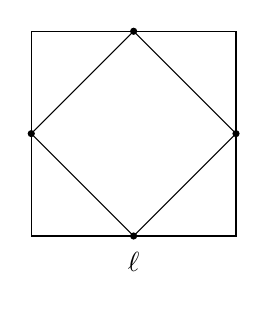
\begin{tikzpicture}[x=1.3cm,y=1.3cm]
\draw (0,0)--(2,0)--(2,2)--(0,2)--cycle;
\draw (1,0)--(2,1)--(1,2)--(0,1)--cycle;
\fill (1,0) circle (1.3pt); \fill (2,1) circle (1.3pt);
\fill (1,2) circle (1.3pt); \fill (0,1) circle (1.3pt);
\node at (1,-.25) {\(\ell\)};
\end{tikzpicture}
\caption{An independently drawn schematic of the source's midpoint-square
problem. The marked points are stipulated midpoints; the picture's physical
size is not the premise establishing the area relation.}
\label{fig:p19-rat133-midpoint-square}
\end{figure}

\begin{hblemma}{thm:p19-rat133-square-area}{proved=annex:p19.rat133-square-area}{Area ratio under exact Euclidean assumptions}
For a Euclidean square of side \(\ell>0\), joining consecutive side
midpoints forms a square. If \(A_{\mathrm{out}}\) and
\(A_{\mathrm{in}}\) are respectively the outer and inner areas, then
\[
             A_{\mathrm{out}}=\ell^2,
\qquad       A_{\mathrm{in}}=\ell^2/2,
\qquad       A_{\mathrm{out}}=2A_{\mathrm{in}}.
\]
The conclusion is general over the stipulated squares, not inferred from
measuring the schematic or a participant's impression.
\end{hblemma}

The diagram's epistemic role can thus be discovery or understanding of an
argument whose conditions are justified separately. Knauff reviews contrasting
mathematical attitudes, associating imagination with Klein and independence
from particular figures with Hilbert. These are attributed positions, not a
proof that visual reasoning is either universally legitimate or universally
unreliable. His discussion of Euler, Venn, Peirce's iconicity and Shin's
formal diagram work likewise distinguishes a formal visual language from an
unregulated inspection of an appealing image
\parencite[pp.~735--736]{Knauff2021VisualizationRationality}.

\subsection{Different external displays can have opposite effects}

Knauff reports Bauer and Johnson-Laird's comparison of sentence-only
conditional problems with conditions also supplied with abstract line diagrams
clarifying logical relations. He reports better performance with those
diagrams. In contrast, his account of Hyperproof studies connects stronger
visualizing tendencies and weaker logic skills with potential benefit from
learning more abstract strategies. Neither report establishes that a learner's
initial preference identifies the most effective format
\parencite[pp.~736--737]{Knauff2021VisualizationRationality}.

Further survey examples compare photographs of real objects with more
abstract, annotated objects in a virtual environment for conditional
reasoning, and discuss route descriptions and photorealistic navigation.
The proposed explanation is that irrelevant detail can compete with
information required by the inference. Multimedia redundancy and seductive
details are neighboring hypotheses: an eye-catching addition can distract
from meaningful learning rather than enhance it. These are distinct tasks
and mechanisms, not one pooled visualization effect
\parencite[p.~737]{Knauff2021VisualizationRationality}.

For these external-display studies the chapter gives qualitative task and
format descriptions but not complete recruitment records, analysis samples,
effect estimates or uncertainty intervals. Their reported directions are
retained as survey claims, not independently quantified here. In particular,
the evidence does not warrant excluding all illustrations, adding all
diagrams, or generalizing one navigation or instructional result to every
logical task. The relevant question is what each representation encodes
and what processing the comparison condition requires.

\section{Internal imagery and the visual impedance hypothesis}
\label{sec:p19-rat133-impedance}

Knauff reviews the imagery debate through historical philosophical positions,
scientific introspection, the W\"urzburg school's reports of imageless
thinking, behaviorist criticism and the later return of representational
accounts. Boltzmann's theoretical imagery and Kekul\'e's reported inspiration
for a cyclic benzene structure are scientific anecdotes, not controlled
evidence that imagery caused discovery or is necessary for deduction.
Perky's imagery/perception confusion and Kosslyn and colleagues' remembered-
island scanning task address other questions: in the latter, response time
to move mentally between landmarks was reported to track map distance.
That does not establish how people validate a logical conclusion
\parencite[pp.~737--738]{Knauff2021VisualizationRationality}.

The visual impedance hypothesis concerns visual detail irrelevant to an
inference. It predicts that selecting the relevant relation from a vivid
picture can add processing, whereas an abstract layout may encode that
relation directly. The contrast is not between sensation and no cognition,
or between images and language as exclusive media.

The competing propositional account treats reasoning as operating on a
language of thought, with visual imagery potentially an epiphenomenon rather
than the inferential medium. Knauff presents the imagery debate as unresolved,
while arguing that content-sensitive interference challenges a simple
picture-inspection account. A formal proof written in sentences does not
show that its human solver used sentence-like internal representations;
likewise, the experience of a picture does not show that the picture performed
the inference \parencite[pp.~736,738]{Knauff2021VisualizationRationality}.

\begin{hbdefinition}{def:p19-rat133-four-classes}{Operational imagery and spatial ratings}
The chapter distinguishes four relation-material classes:
\begin{center}
\begin{tabular}{lll}
Class & Easy to envisage visually & Easy to envisage spatially\\ \hline
visuospatial & yes & yes\\
visual & yes & no\\
spatial & no & yes\\
abstract/control & no & no
\end{tabular}
\end{center}
These are classifications under a rating procedure, not intrinsic immutable
properties of words or people. Above/below can suggest a spatial order;
cleaner/dirtier can elicit pictorial detail not needed to compare positions
on an abstract scale. The original experiments call their low-visual,
low-spatial comparison materials \emph{control relations}; the 2021 chapter
also calls that class abstract.
\end{hbdefinition}

\subsection{The original 2002 experiments: measures and boundaries}

Knauff and Johnson-Laird first asked ten native-English-speaking Princeton
student volunteers to rate assertions on separate seven-point visual and
spatial scales. They identified visuospatial, visual and control relation
pairs, controlling word frequency and swapping the same animal nouns. An
initial German norming study with twelve Freiburg students still did not
isolate purely spatial pairs. A later twenty-student bipolar visual/spatial
rating procedure selected north/south and ancestor/descendant materials.
Thus the four-class description emerged through different norming procedures;
it is not a single successful orthogonal manipulation of two independent
subjective scales \parencite[pp.~364--368]{KnauffJohnsonLaird2002VisualImpedance}.

\paragraph{Participants, tasks and comparisons.}
Experiment~1 tested 22 Princeton undergraduates for course credit, mean age
19.5, twelve female and ten male. Each evaluated 24 randomly ordered
three- or four-term transitive inferences using visual, visuospatial or
control relations; half the proposed conclusions were valid.
Experiment~2 used twenty new students from the same population, 24
conditional/transitive problems, and four arrangements of a relation and
its converse to manipulate difficulty. Experiment~3 tested 24 Freiburg
undergraduates, mean age 22.4, fourteen female and ten male, paid or given
credit. They evaluated 32 three- or four-term problems with all four classes
using German spatial expressions
\parencite[pp.~365--368]{KnauffJohnsonLaird2002VisualImpedance}.

All were within-participant comparisons. Premises appeared separately in
black text, then a proposed conclusion in red; presentation was self-paced.
Participants judged necessary consequence with keyboard responses after
four practice problems. The computer recorded premise-reading times,
answers and conclusion-response latency. These were verbally specified
relations, not comparisons between showing and withholding external pictures.
No probability-recruitment frame or prospective power calculation is reported.

\begin{table}[htbp]
\centering\small
\begin{tabular}{lrrrr}
 & visual & control & visuospatial & spatial\\ \hline
Exp.~1 correct (\%) &86&92&90&\text{not tested}\\
Exp.~1 correct-response \(\mathrm{RT}\) (s)&2.65&2.38&2.20&\text{not tested}\\
Exp.~2 correct (\%)&77&67&68&\text{not tested}\\
Exp.~2 correct-response \(\mathrm{RT}\) (s)&3.37&2.64&2.46&\text{not tested}\\
Exp.~3 correct (\%)&73&78&72&72\\
Exp.~3 correct-response \(\mathrm{RT}\) (s)&4.48&3.81&3.74&3.52
\end{tabular}
\caption{Original 2002 Table~2 summaries. Latencies concern correct
responses, not all responses or a separately observed imagery-operation
duration. The article supplies no confidence intervals for these cell means.}
\label{tab:p19-rat133-original-outcomes}
\end{table}

In each experiment, visual relations reliably slowed correct responses.
Experiments~1 and~2 report visual-versus-control Wilcoxon comparisons of
\(z=3.07,p<.002\) and \(z=2.46,p<.02\), respectively; Experiment~3
reports visual slowing relative to the other three classes
\((z=2.46,p<.015)\).
The predicted latency order was supported, but the direct visuospatial or
spatial speedups over controls were not significant. Accuracy differences
among relation classes were not significant in any of the three experiments.
The original supports visual latency impedance, not the claim that these
same experiments demonstrated more reasoning errors or an established
pure-spatial advantage \parencite[pp.~365--369]{KnauffJohnsonLaird2002VisualImpedance}.

Reading and conclusion times must also be distinguished. Experiment~3's
spatial premises took relatively long to read, particularly the less frequent
north/south terms, despite the low conclusion latency in that condition.
The authors discuss frequency, interpretation of transitivity and plausibility
as alternative influences. They balanced converse relations and fixed nouns,
but such controls do not turn introspective ratings into a direct measurement
of the mediating representation. The samples are small student cohorts;
the language and material differences limit transfer between experiments
and beyond their tasks \parencite[pp.~368--370]{KnauffJohnsonLaird2002VisualImpedance}.

The 2021 chapter's broader accuracy claim cites other work as well, rather
than being discharged by the 2002 study alone. It also reports individual
differences based on verbalizer--visualizer questionnaires, reading-deficit
groups, congenitally blind participants and minimally invasive surgery
training. Those findings concern different populations, measures and tasks;
they are not replications of one shared numerical effect
\parencite[pp.~738--739]{Knauff2021VisualizationRationality}.

\section{Neural evidence: distinguish phases, contrasts and interpretations}
\label{sec:p19-rat133-neural}

Knauff reports a distributed frontal, temporal and parietal reasoning network,
with additional visual-region activity for some imagery-provoking materials.
The chapter's Figure~13.3.2 distinguishes premise processing, integration
and conclusion evaluation. Its phase rows display cortical activation patterns,
not the visual content of thought, rates of correct inference or proof that
any one region alone implements rationality
\parencite[pp.~739--740]{Knauff2021VisualizationRationality}.

\paragraph{The original 2006 record behind the figure.}
Fangmeier and colleagues tested twelve right-handed male undergraduate and
graduate students, mean age 22.4 (SD 1.98), with normal or corrected vision
and no reported neurological/psychiatric disorder or significant drug abuse.
They used 32 spatial reasoning problems and 32 matched maintenance problems
in four pseudorandomized scanner runs. Premises and queries were sequences
of letters \(V,X,Z\) placed left or right of the screen center rather than
ordinary-language sentences. The reasoning response judged whether a new
relation followed; the maintenance response judged whether the query
repeated a previous premise. Pre-scanner training used twelve problems to
reach at least 75\% accuracy
\parencite[pp.~321,330--332]{FangmeierEtAl2006ThreeStage}.

Each letter appeared for 1500~ms, followed by another letter for 1500~ms
and a 1000-ms pause; each premise or query thus occupied 4000~ms.
The design sought to hold visual material and memory load fixed while
contrasting integration/validation demands. Responses used an MRI-compatible
box. The study measured response accuracy and latency, event-related BOLD
signals and a post-scan Block Design Test. The behavioral comparison was
91\% correct for reasoning versus 97\% for maintenance
\((Z=2.31,p=.021)\), with mean latencies 3021 versus 2843~ms
\((Z=-2.04,p=.041)\). No confidence interval for these differences is
printed \parencite[pp.~322,330--332]{FangmeierEtAl2006ThreeStage}.

The original describes early \emph{occipito-temporal and visual association}
activity, anterior prefrontal involvement in integration, and prefrontal
plus posterior-parietal activity in validation. This is the anatomical
scope of the OTC labels in the chapter figure, not a demonstrated V1-only
or primary-visual-cortex result. Reasoning-minus-maintenance contrasts
identified greater anterior-prefrontal activity in the second phase and
prefrontal/right-precuneus activity in the third. They do not show that
every other region is inactive or that inference occurs only after premise
integration \parencite[pp.~322--330]{FangmeierEtAl2006ThreeStage}.

The analysis used correct trials, SPM99 random-effects comparisons, a
height threshold \(t=3.0\) and cluster-level multiple-comparison correction
for reported within-condition clusters. An additional response-time regressor
addressed task-difficulty differences without removing the reported central
contrasts. The published methods specify different within-phase and
between-condition contrasts; a thresholded map is not a direct movie of
three isolated mental operations. The sample was all male, right-handed,
student volunteers, with Block Design scores in a restricted normal-to-
superior range. Reverse inference from a region to a unique representation,
selection of only correct trials and unequal task difficulty remain material
interpretative limits. The authors themselves caution that other problem
types can elicit other processes
\parencite[pp.~322--330,332]{FangmeierEtAl2006ThreeStage}.

\begin{proofboundary}{def:p19-rat133-clinical-boundary}{Survey extensions are not treatment, diagnosis or etiology}
The chapter reports visual-cortex TMS facilitating some reasoning tasks and
parietal TMS impairing others, and interprets a blind-participant comparison
as evidence against a need for pictorial imagery. It also mentions lorazepam,
autism-related reports and reading-deficit studies. These are not all the
same manipulation or population. The chapter does not provide the complete
sample/design/intensity/control/effect/uncertainty record for each, and those
original studies are not independently quantified in this entry.

In particular, a reasoning-performance comparison involving dyslexic readers
does not by itself establish that imagery is a main cause of dyslexia; that
strong etiological suggestion in the survey is not adopted here. An
autobiographical report, questionnaire grouping or congenital-blindness
comparison does not randomly assign a mental representation. Neither a
drug nor a TMS report is a recommendation to intervene to improve reasoning.
Grandin's \emph{Thinking in Pictures} is the source's autobiographical
illustration of helpful visual practice alongside difficulty with abstraction,
not a controlled estimate for autistic people generally.
\end{proofboundary}

This preserves the chapter's reported contrasts without promoting them
to universal clinical or causal conclusions
\parencite[pp.~735,738--739]{Knauff2021VisualizationRationality}.

\section{Computational explanations and the preferred-model boundary}
\label{sec:p19-rat133-models}

Knauff's computational examples distinguish a display or image-processing
program from an explanation of human inference. WHISPER manipulated
blocks-world diagrams; Kosslyn and Shwartz used metrically located contents
in filled/unfilled matrix cells. Berendt's imagery model reconstructed some
preferences for interpretations of ambiguous premises, while Schlieder's
more parsimonious representation retained the ordering of endpoints rather
than extensive visual detail. The comparison asks which information and
operations are needed to reproduce a specified response pattern, not which
picture looks most natural \parencite[p.~740]{Knauff2021VisualizationRationality}.

PRISM represents tokens in an abstract spatial array with a movable focus,
construction, inspection and variation operations. A preferred model can
support a quick answer while omitting other satisfying arrangements.
The actual original implementation and its limits are treated in
\cref{sec:p19-rat132-prism}: its descriptive search policy does not routinely
seek a counterexample to a query already true in the preferred model, and
its defaults are not every proposed working-memory limitation.
Thus an erroneous necessity judgment can be modeled without declaring it
logically valid. The 2021 visualization chapter also points to preliminary
computational simulations of impedance, explicitly leaving algorithmic
details open \parencite[pp.~740--741]{Knauff2021VisualizationRationality}.

\section{Corollaries, comparisons and task lookup}
\label{sec:p19-rat133-lookup}

Knauff's six concluding claims form an argument with distinct evidential
strengths. First, introspection can misidentify the process producing an
answer. Second, a descriptive theory must explain errors as well as
normatively successful answers. Third, he argues that imagery can causally
impede inference, proposing a detour through visual processing before
abstract relational work; the particular detour is an explanatory hypothesis,
not a uniquely identified algorithm. Fourth, imagery's educational value
depends on task and representation rather than vividness alone. Fifth,
external detail can elicit internal imagery, making relevance and overload
important. Sixth, logical reasoning is a special domain, so transfer to all
thinking is not established \parencite[p.~741]{Knauff2021VisualizationRationality}.

\begin{hbmethod}{def:p19-rat133-evaluate-aid}{Evaluate the representation against its actual reasoning task}
\begin{enumerate}
\item Fix the query and correctness criterion: memory, identity under rotation,
      feature binding, possibility, necessity, learning or proof.
\item Specify the encoding, viewpoint, scales and incidental visual features.
      Separate external format from any hypothesis about internal imagery.
\item Check whether a proposed inference is warranted by the encoded premises,
      including alternatives not displayed in a preferred arrangement.
\item Compare representations with declared participants, materials, controls
      and instructions. Measure accuracy, reading/encoding time and response
      latency separately when the explanation depends on that distinction.
\item Report uncertainty, negative as well as positive comparisons, and
      possible confounds such as language, semantic content, word frequency,
      prior skill, speed--accuracy tradeoffs and difficulty.
\item Test transfer rather than inferring it from appeal, preference or local
      success. A new population or unaided task is a new evidential question.
\end{enumerate}
This procedure implements the representational and evidence distinctions
above; it is not a theorem that abstract displays always outperform concrete
ones. The evidence-reporting interface is \cref{def:p19-evidence-record}.
\end{hbmethod}

A successful lookup use identifies why the midpoint diagram suggests a
general relation and supplies the exact geometrical justification, or
interprets the 2002 latency effect under its actual materials and samples.
A failed use infers universal validity from one pleasing picture, treats
slowing as automatically more errors, infers V1 or an exact mental algorithm
from a thresholded association map, or claims general rationality training
from a local display benefit.

Logical diagrams in \cref{sec:p12-rationality-13-1} have declared syntax,
semantics and proof obligations; this chapter studies assistance and
interference in using representations. Spatial/temporal reasoning in
\cref{sec:p19-rationality-13-2} concerns relational constraints and
preferred-model procedures; this chapter separates those abstract relations
from pictorial detail. Mental rotation in \cref{sec:p19-mental-rotation}
compares geometric identity responses across disparities, while its
feature-binding studies measure retention of color-to-part correspondences
during transformation. Neither is the 2002 necessary-consequence task or
the 2006 reasoning-versus-maintenance contrast. Compatible findings across
these tasks can constrain explanations without becoming one common
visualization effect or a universal measure of rationality.

\chapter{Rationality and Intelligence}
\label{sec:p19-rationality-15-2}

An intelligence score and a judgment about rational thinking need not assess
the same thing. Stanovich, Toplak and West's chapter~15.2 compares them as
individual-difference constructs in cognitive science. It adopts a grounded
account of what intelligence tests measure, then argues that rational
responding additionally depends on dispositions to initiate reflection and
on learned knowledge and strategies. Its tripartite architecture explains
how substantial computational ability can coexist with poorly supported
beliefs or injudicious decisions
\cite[pp.~791--800]{StanovichToplakWest2021Intelligence}.

This is a specified psychological comparison, not a universal definition of
rationality, an assessment of someone's worth, or a diagnostic rule derived
from an IQ score. The source reconstructs a cognitive architecture and
reviews qualitative individual-difference findings. It does not provide
participant-level methods, correlation tables or a standardized rationality
test with a complete scoring manual in this chapter. Its four figures are
functional models, not measured maps of three anatomically separate modules.

\section{Match the construct to its measurement}
\label{sec:p19-rat152-constructs}

\begin{hbdefinition}{def:p19-rat152-grounding}{Grounded intelligence and individual-difference rationality}
A permissive conception of intelligence includes whatever the broad everyday
word suggests, such as adaptation, wisdom or creativity, whether or not
existing IQ tests measure those capacities. The source's grounded conception
instead anchors intelligence to the abilities assessed by the tests being
discussed. In the Cattell--Horn--Carroll account, general intelligence is
conventionally denoted \(g\), with broad factors including fluid and
crystallized intelligence.

Fluid intelligence concerns reasoning across domains, including unfamiliar
ones; the chapter names figural analogies, Raven matrices and series
completion as measurement families. Crystallized intelligence concerns
knowledge acquired through acculturated learning; vocabulary, verbal
comprehension and general knowledge are its named measurement families.
These names identify constructs and task families, not a locally supplied
test battery or interchangeable measures of every reasoning skill.

Rationality in this comparison concerns individual differences in responses
evaluated against stated normative models. The relevant departure is from
the specified model's standard, not from a researcher's personal preference.
The concept must be assessed at a grain comparable to the individual-difference
concept of intelligence. An all-or-nothing philosophical attribution of
rational agency answers a different question.
\index{intelligence!rationality distinction}
\index{rationality!individual differences}
\index{mindware}
\end{hbdefinition}

The source opens with the apparent paradox of someone described as smart
acting foolishly. If both words refer to intellectual capacity, the phrase
appears contradictory. If the second description instead concerns poor
decisions or careless errors, it distinguishes capacity from judicious
deployment. The dictionary illustration identifies an ambiguity; it does
not supply an empirical frequency of high-IQ mistakes. Adopting a broad
definition that includes wise decisions does not make an existing IQ test
measure that additional property
\cite[secs.~1--2, pp.~791--792]{StanovichToplakWest2021Intelligence}.

The authors characterize CHC as a well-supported grounded framework and
argue that fluid and crystallized abilities leave important rationality
components unmeasured. This is their theoretical and measurement claim,
not the proposition that intelligence is unrelated to reasoning performance.
Test labels alone also do not show that a score is a pure measure of one
process: language, schooling, prior exposure, motivation, task instructions
and measurement error can affect an observed score. Such influences must
be investigated rather than inferred away by calling a test an ability test.

\section{Normative standards and task-specific scoring}
\label{sec:p19-rat152-benchmarks}

The chapter distinguishes epistemic rationality, concerning how beliefs
match the world, from instrumental rationality, concerning achieving one's
goals with the available physical and mental resources. Its more formal
instrumental comparison is expected-utility maximization: weight each
possible outcome's utility by its probability and add the products.
Direct experimental assessment is difficult when personal probabilities
and utilities are hard to elicit. The axiomatic alternative evaluates
patterns of preference against conditions that support an as-if utility
representation \cite[p.~792]{StanovichToplakWest2021Intelligence}.

That representation requires the actual preference domain and axioms.
\Cref{sec:p17-finite-expected-utility} supplies a complete finite-prize
lottery representation under its mixture, continuity and preference
assumptions; the simpler ordinal theorem on a finite set is not sufficient
for all those lottery comparisons. An as-if representation is not a proof
that someone consciously multiplied utilities, a warrant for arbitrary
payoff assignments, or a guarantee of favorable realized outcomes. A
chance outcome can be unlucky after a choice maximizing the stipulated
expected value.

The source's operational task families include probability assessment,
hypothesis testing, utility-axiom consistency, calibration, resistance
to irrelevant contextual influences and consideration of an alternative
hypothesis. The heuristics-and-biases tradition supplies many of those
operationalizations. They can draw on cognitive capacity without exhausting
what an IQ test measures. Their responses also require the relevant learned
knowledge, interpretation and opportunity to apply it.

\begin{hbexample}{def:p19-rat152-scoring-contrast}{Different measures require different criteria}
A figural-analogy item can be scored against its designated completion
rule under instructions to find the correct option. A probability judgment
instead requires a specified event and interpretation; a calibration
judgment additionally requires a collection or law relating reports to
outcomes. As \cref{def:p19-calibration-law} shows, correctness of selected
answers and calibration of confidence are not the same score.

Similarly, a changed preference between two descriptions of the same lottery
is a framing inconsistency only if the descriptions preserve all consequences
and probabilities relevant to the comparison. If one changes information,
timing, social consequences or costs that matter to the person, the premise
of equivalence is not established. A hypothesis-testing answer needs its
alternative hypotheses and the aim of the test specified before it is
called inefficient.

These are stipulated scoring contrasts based on the source's actual task
families, not a newly validated psychometric scale. They do not permit
adding an analogy score, a confidence error and a preference violation
into one rationality quotient without a justified measurement model.
\end{hbexample}

The chapter describes degrees of rationality in terms of distance from a
normative optimum but supplies no single distance function, common unit,
item weighting or population norm covering all these tasks. A proportion
of answers matching a key, a calibration score and a choice-axiom violation
therefore retain their own interpretation. The theoretical argument that
rationality can be measured does not itself provide a complete instrument
or a legitimate threshold for classifying individuals.

\section{The preliminary dual-process architecture}
\label{sec:p19-rat152-dual}

\begin{hbdefinition}{def:p19-rat152-process-types}{Autonomy, override and cognitive decoupling}
In the source's Type~1/Type~2 terminology, autonomy is the defining feature
of Type~1 processing: encountering its triggering conditions initiates it
without a high-level control instruction. Rapid, associative, low-central-load
processing commonly accompanies autonomy but does not define the category.
Many autonomous processes can operate in parallel. Mandatory triggering
does not mean that the resulting response must be emitted without override.

Type~2 processing is nonautonomous and comparatively demanding, with largely
serial use of central resources. It can interrupt a Type~1 response and
simulate an alternative. Cognitive decoupling keeps a hypothetical situation
distinct from the represented actual world while the simulation proceeds.
Representing a premise for purposes of reasoning is not necessarily believing
that premise true of the world.
\end{hbdefinition}

The chapter's preliminary model gives Type~2 a response path and a simulation
path, while Type~1 has its own response path. Preattentive Type~1 computations
also supply input to Type~2. Figure~\ref{fig:p19-rat152-preliminary}
re-presents those source connections. The presence of an override route
does not entail that the autonomous proposal is always wrong. A heuristic
can be adaptive in an environment with suitable cues and costly in an
environment where those cues mislead
\cite[sec.~3, pp.~792--794, fig.~15.2.1]{StanovichToplakWest2021Intelligence}.

\begin{figure}[htbp]
\centering
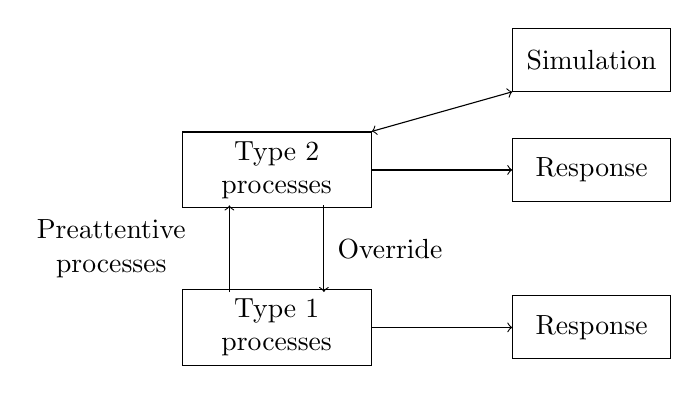
\begin{tikzpicture}[x=1cm,y=1cm]
\node[draw,minimum width=2.4cm,minimum height=.9cm,align=center] (t2) at (0,2) {Type 2\\processes};
\node[draw,minimum width=2.4cm,minimum height=.9cm,align=center] (t1) at (0,0) {Type 1\\processes};
\node[draw,minimum width=2cm,minimum height=.8cm] (sim) at (4,3.4) {Simulation};
\node[draw,minimum width=2cm,minimum height=.8cm] (r2) at (4,2) {Response};
\node[draw,minimum width=2cm,minimum height=.8cm] (r1) at (4,0) {Response};
\draw[<->] (t2.north east)--(sim.south west);
\draw[->] (t2.east)--(r2.west);
\draw[->] (t1.east)--(r1.west);
\draw[->] (-.6,.45)--(-.6,1.55);
\node[align=center] at (-2.1,1) {Preattentive\\processes};
\draw[->] (.6,1.55)--(.6,.45);
\node[right] at (.65,1) {Override};
\end{tikzpicture}
\caption{Native vector reconstruction of the source's preliminary
dual-process model, Figure~15.2.1. Arrows describe proposed functional
connections, not estimates of process strength, duration or brain location.}
\label{fig:p19-rat152-preliminary}
\end{figure}

The source acknowledges multiple dual-process theories and occasionally
uses the similar System~1/System~2 labels. That terminology must not hide
the heterogeneity of autonomous processes or turn speed into a sufficient
classification rule. \Cref{sec:p19-rationality-2-5} develops the broader
dual-process debate and its task-specific evidence; the present chapter
uses the architecture to distinguish kinds of individual differences.

\section{Two levels within Type 2: ability and disposition}
\label{sec:p19-rat152-tripartite}

\begin{hbdefinition}{def:p19-rat152-levels}{Algorithmic and reflective functions}
The algorithmic mind carries out processing: suppressing a triggered
response, sustaining a decoupled representation and computing an alternative.
The reflective mind initiates and regulates those activities in relation to
goals and epistemic commitments. Possessing an operation and initiating it
when appropriate are different proposed functions.

The chapter links variation in fluid intelligence primarily to algorithmic
processing efficiency and variation in thinking dispositions to reflective
control. Thinking dispositions include actively open-minded thinking,
need for cognition, consideration of future consequences, need for closure
and dogmatism. Those constructs and their directions of desirability must
be assessed using specified instruments; listing them does not provide
their scoring keys.
\end{hbdefinition}

The source's psychometric contrast is between maximal and typical
performance. In a maximal-performance assessment, the task interpretation
and goal are externally specified and the participant is asked to do as well
as possible. In a typical-performance assessment, goal selection and usual
epistemic regulation enter the observed behavior. The authors classify
intelligence/aptitude tests with maximal performance and many rational- or
critical-thinking measures with typical performance. This is a distinction
about assessment demands, not evidence that every aptitude-test response
is unaffected by willingness or that a disposition questionnaire is a
pure measure of behavior.

\begin{figure}[htbp]
\centering
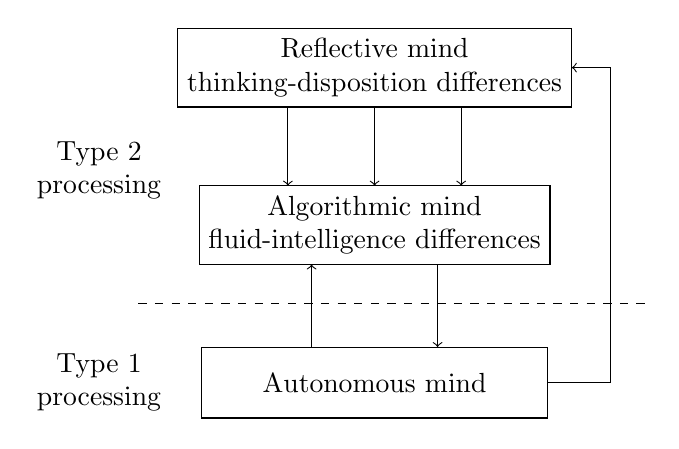
\begin{tikzpicture}[x=1cm,y=1cm]
\node[draw,minimum width=4.4cm,minimum height=1cm,align=center] (ref) at (0,4) {Reflective mind\\thinking-disposition differences};
\node[draw,minimum width=4.4cm,minimum height=1cm,align=center] (alg) at (0,2) {Algorithmic mind\\fluid-intelligence differences};
\node[draw,minimum width=4.4cm,minimum height=.9cm] (aut) at (0,0) {Autonomous mind};
\foreach \x in {-1.1,0,1.1}{\draw[->] (\x,3.5)--(\x,2.5);}
\draw[->] (-.8,.45)--(-.8,1.5);
\draw[->] (.8,1.5)--(.8,.45);
\draw[->] (aut.east)--(3,0)--(3,4)--(ref.east);
\draw[dashed] (-3,1)--(3.5,1);
\node[align=center] at (-3.5,2.7) {Type 2\\processing};
\node[align=center] at (-3.5,0) {Type 1\\processing};
\end{tikzpicture}
\caption{Native reconstruction of Figure~15.2.2. The older Type~1/Type~2
division is the dashed boundary; the added reflective/algorithmic division
is within Type~2. Distinct explanatory roles are not a claim that the
associated measured traits are statistically independent.}
\label{fig:p19-rat152-tripartite}
\end{figure}

Under explicit instructions a participant might correctly compare alternative
hypotheses, yet normally settle on a familiar explanation without making
that comparison. The difference could concern initiation rather than an
inability to perform the operation. Conversely, willingness to reconsider
does not ensure knowledge of the needed rule or sufficient processing
capacity. This is an explanatory contrast permitted by the model, not
an observation of a particular participant's unmeasured mental process.

The source links fluid intelligence, executive function and working memory
to maintaining decoupled simulations. It reports substantial association,
not numerical coefficients or a primary experiment here. A working-memory
score is not direct observation of a decoupling operation. The proposed
link requires a theory connecting the tasks and competing explanations,
not just a shared correlation
\cite[secs.~4--5, pp.~794--795]{StanovichToplakWest2021Intelligence}.

\section{The complete functional model and its limits}
\label{sec:p19-rat152-functions}

The source's Figure~15.2.3 decomposes the routes more precisely. A is
algorithmic override of the autonomous output; B is the reflective
instruction to initiate that override. C is algorithmic decoupling into
simulation; D is the reflective instruction to initiate it. E is serial
associative cognition, and F is a reflective change of control over that
sequence. G denotes preattentive input to higher control. The reflective
initiation calls and the computations they initiate must not be compressed
into one ability variable.

\begin{figure}[htbp]
\centering
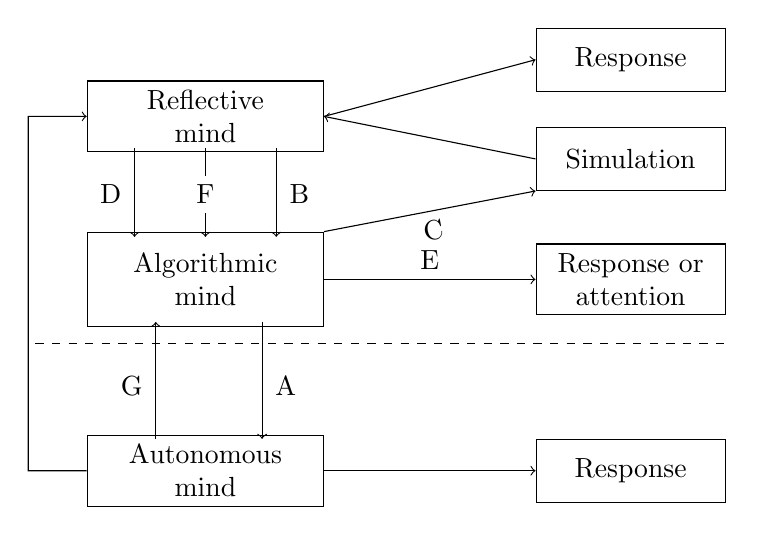
\begin{tikzpicture}[x=1cm,y=1cm,scale=.9]
\node[draw,minimum width=3cm,minimum height=.9cm,align=center] (ref) at (0,5) {Reflective\\mind};
\node[draw,minimum width=3cm,minimum height=1.2cm,align=center] (alg) at (0,2.7) {Algorithmic\\mind};
\node[draw,minimum width=3cm,minimum height=.9cm,align=center] (aut) at (0,0) {Autonomous\\mind};
\node[draw,minimum width=2.4cm,minimum height=.8cm] (rr) at (6,5.8) {Response};
\node[draw,minimum width=2.4cm,minimum height=.8cm] (sim) at (6,4.4) {Simulation};
\node[draw,minimum width=2.4cm,minimum height=.9cm,align=center] (ra) at (6,2.7) {Response or\\attention};
\node[draw,minimum width=2.4cm,minimum height=.8cm] (r1) at (6,0) {Response};
\draw[->] (ref.east)--(rr.west);
\draw[->] (sim.west)--(ref.east);
\draw[->] (alg.north east)--node[below,sloped]{C}(sim.south west);
\draw[->] (alg.east)--node[above]{E}(ra.west);
\draw[->] (aut.east)--(r1.west);
\draw[->] (-1,4.55)--(-1,3.3);
\node[left] at (-1.05,3.9) {D};
\draw[->] (0,4.55)--(0,3.3);
\node[fill=white] at (0,3.9) {F};
\draw[->] (1,4.55)--(1,3.3);
\node[right] at (1.05,3.9) {B};
\draw[->] (-.7,.45)--(-.7,2.1);
\node[left] at (-.75,1.2) {G};
\draw[->] (.8,2.1)--(.8,.45);
\node[right] at (.85,1.2) {A};
\draw[->] (aut.west)--(-2.5,0)--(-2.5,5)--(ref.west);
\draw[dashed] (-2.4,1.8)--(7.4,1.8);
\end{tikzpicture}
\caption{Independent native layout of the complete proposed connections in
Figure~15.2.3, retaining arrows A--G and both autonomous input routes.
The processing/initiating distinction is substantive; node position is
illustrative rather than a neural localization.}
\label{fig:p19-rat152-functions}
\end{figure}

The F instruction can stop a serial association to begin a comprehensive
simulation, or redirect the sequence from another starting point. The
chapter does not develop the full function of serial associative cognition;
it refers to Stanovich's 2011 treatment. An arrow naming that function
does not supply the unprinted complete mechanism. Likewise, the source's
use of hierarchical brain control is a functional explanation, not an
empirical demonstration that each diagram node occupies one brain region
\cite[sec.~6, pp.~795--796]{StanovichToplakWest2021Intelligence}.

\subsection{Mindware and two routes to a normative response}

Perkins's term mindware denotes available learned knowledge, rules,
procedures and strategies used to transform a hypothetical representation.
The chapter emphasizes specialized probabilistic, causal and scientific
knowledge. Ordinary crystallized-intelligence measures broadly sample
vocabulary and general knowledge rather than directly testing all those
specialized resources. A learner can therefore know many words without
knowing an appropriate method for interpreting base rates; knowing the
method also does not ensure applying it.

Some learned rules can become automatic through extensive practice.
Figure~\ref{fig:p19-rat152-mindware} preserves both source routes: accessing
mindware during demanding simulation, and practiced mindware residing
within autonomous processing. Consequently, a response matching a normative
criterion does not uniquely identify Type~2 as its origin. The rule might
have been applied automatically; an erroneous response can instead follow
prolonged deliberate computation with missing or unsuitable knowledge.

\begin{figure}[htbp]
\centering
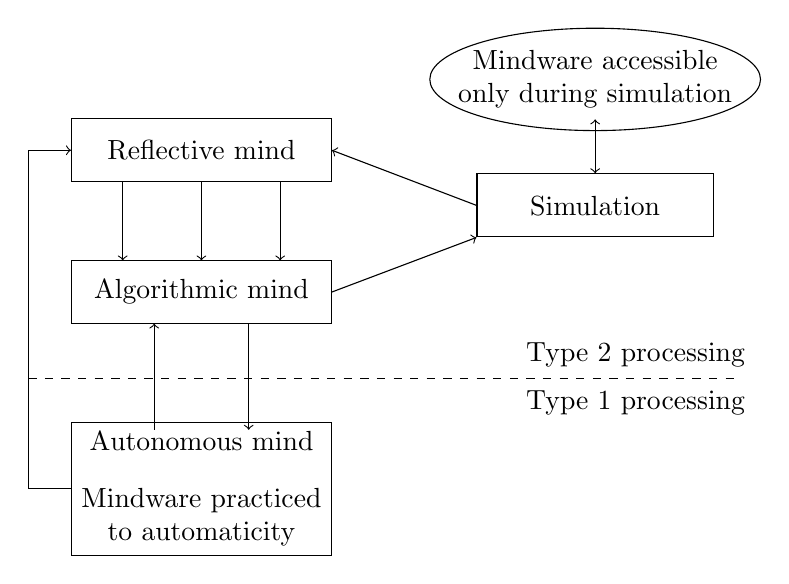
\begin{tikzpicture}[x=1cm,y=1cm]
\node[draw,minimum width=3.3cm,minimum height=.8cm,align=center] (ref) at (0,4.3) {Reflective mind};
\node[draw,minimum width=3.3cm,minimum height=.8cm,align=center] (alg) at (0,2.5) {Algorithmic mind};
\node[draw,minimum width=3.3cm,minimum height=1.5cm,align=center] (aut) at (0,0) {Autonomous mind\\[.3cm]Mindware practiced\\to automaticity};
\node[draw,minimum width=3cm,minimum height=.8cm] (sim) at (5,3.6) {Simulation};
\draw (5,5.2) ellipse (2.1 and .65);
\node[minimum width=3.3cm,minimum height=1cm,align=center] (mw) at (5,5.2) {Mindware accessible\\only during simulation};
\foreach \x in {-1,0,1}{\draw[->] (\x,3.9)--(\x,2.9);}
\draw[->] (-.6,.75)--(-.6,2.1);
\draw[->] (.6,2.1)--(.6,.75);
\draw[->] (aut.west)--(-2.2,0)--(-2.2,4.3)--(ref.west);
\draw[->] (alg.east)--(sim.south west);
\draw[->] (sim.west)--(ref.east);
\draw[<->] (sim.north)--(mw.south);
\draw[dashed] (-2.2,1.4)--(6.8,1.4);
\node[right] at (4,1.7) {Type 2 processing};
\node[right] at (4,1.1) {Type 1 processing};
\end{tikzpicture}
\caption{Native re-presentation of Figure~15.2.4. Autonomous practiced
mindware and simulation-accessible mindware have different routes to
responding. A correct response alone cannot choose between the routes.}
\label{fig:p19-rat152-mindware}
\end{figure}

The source concludes that rational responding can require three classes
of characteristics: computational capacity for override and sustained
simulation, reflective dispositions to initiate useful operations, and
available/accessibly learned mindware, including automatic rules. This is
why its rationality construct is broader than the intelligence construct
it operationalizes. It is not the claim that all three operations occur
in every item or that deliberating longer always improves an answer
\cite[pp.~796--798, fig.~15.2.4]{StanovichToplakWest2021Intelligence}.

\section{Individual-difference claims and their evidence boundary}
\label{sec:p19-rat152-evidence}

The chapter reports that intelligence and thinking dispositions are not
perfectly associated. It describes moderate-to-weak relationships for some
dispositions, including actively open-minded thinking and need for cognition,
and near-zero relationships for others, including conscientiousness,
curiosity and diligence, citing review sources. It further reports that
thinking dispositions predict task variation after general intelligence
is controlled. In this chapter these are qualitative literature reports:
the samples, exact instruments, coefficients, intervals and adjustment
models are not given \cite[sec.~5, p.~795]{StanovichToplakWest2021Intelligence}.

Those claims support the authors' proposal that capacity and regulation
should not be treated as one measured variable. They do not justify
declaring the traits independent, a fixed numerical relation across all
populations, or that an intelligence score predicts a particular person's
judgment. Imperfect measured association can involve measurement error,
restriction of range, differing task demands, prior knowledge or population
selection as well as distinct psychological functions. A residual association
after a selected adjustment is not an experimentally isolated causal effect.

The review's reports about working memory/executive function and its claim
that cognitive ability often, but not always, dissociates from an
evolutionarily characterized modal response have the same source boundary.
No original 1998/1999 dataset or more-than-100-year intelligence history
is reconstructed from a reference citation alone. A strong empirical account
would specify the recruited and analyzed populations, instruction and
scoring versions, repeated observations, reliability, selection, uncertainty
and plausible alternatives, as required by \cref{def:p19-evidence-record}.

\begin{hbwarning}{def:p19-rat152-metric-boundary}{No universal rationality or clinical classification from these diagrams}
Neither \(g\), an IQ score, a thinking-disposition questionnaire nor one
bias task supplies a universal diagnostic measure of rationality. The source's
architectural claims concern specified individual differences and tasks.
They do not license inferring a disorder, fixed incapacity, moral failing
or a population prevalence from an individual answer. A high ability score
does not establish that the relevant reflection occurred; a low score does
not prove that a response violates its stated norm.
\end{hbwarning}

\section{The Great Rationality Debate: what the reconciliation assumes}
\label{sec:p19-rat152-debate}

The authors call one pole Meliorist: observed departures from normative
standards leave room for improvement through education and information.
They call the other Panglossian: the modal response may reflect a suitable
task interpretation or an adaptive information-processing strategy, so
maximal rationality should be a starting presumption. They associate
philosophical, evolutionary, ecological and Bayesian contributions with
the latter pole. These labels organize their debate; they do not show
that every named contributor endorses one identical theory or that every
observed minority answer is normatively better
\cite[sec.~7, pp.~798--799]{StanovichToplakWest2021Intelligence}.

Their proposed reconciliation combines individual-difference patterns with
the differentiated architecture. It distinguishes evolutionary fitness
at the subpersonal genetic level from utility/goal satisfaction at the
personal level. A response favored in an ancestral environment can be
common without best serving an individual's present goals in a different
environment. In the source's proposal, more flexible Type~2 control can
override such a response when the outputs conflict; this makes evolutionary
adaptiveness and personal instrumental or epistemic success different
assessment criteria. References to genes' goals describe an evolutionary
explanatory level, not conscious desires of genes.

The source also invokes a triangulating pattern: higher cognitive ability
is often associated with the response classified as rational for the
individual rather than with the response characterized as evolutionarily
adaptive. It reports exceptions and refers to fuller 1998--2000 studies
and Stanovich's 2004 argument. Those are cited premises of its reconciliation,
not numerical results independently verified here. A response's correlation
with intelligence alone cannot settle the correct normative model; the
model's task interpretation, probabilities, consequences and goals require
their own defense. Nor is ancestral adaptiveness proof of a duty to repeat
the response today.

The architecture itself allows automatic normative mindware and deliberate
error. Therefore its reconciliation cannot consistently be read as
``Type~1 is irrational, Type~2 is rational'' or as a universal instruction
to override intuition. Benign versus hostile cue environments, individual
versus subpersonal goals, relevant knowledge and the costs of deliberation
all condition the proposal. The chapter offers a theory-driven rapprochement,
not a completed proof of the historical or evolutionary claims in every
source it cites.

\section{Development, monitoring, training and consultation}
\label{sec:p19-rat152-use}

\Cref{sec:p19-rationality-15-1} distinguishes explicit metalogical
understanding from the adequacy of inferences actually produced. That
developmental distinction is compatible with separating ability from its
deployment, but childhood cohort comparisons do not supply the adult
intelligence/disposition correlations absent here. Correct deduction,
an explanation of logical necessity and a usual willingness to reflect
remain distinct outcomes.

Monitoring and control in \cref{def:p19-r86-monitoring-control} separate
an answer, a judgment about its adequacy and a decision to persist or stop.
The tripartite model supplies possible computational/control roles; a
confidence rating is not itself an intelligence measure or proof of
reflective engagement. The metacognition chapter's labor-in-vain contrast
also prevents replacing rationality by total time spent thinking.

\Cref{sec:p19-rationality-15-3} distinguishes instructed performance,
retained learning, transfer to new tasks and improved real-life outcomes.
Practiced mindware is a mechanism proposed in 15.2, not an intervention
effect measured by its diagrams. Evidence that a training program improves
one task must establish its own population, control conditions and transfer
outcomes. A higher score after practice might reflect item familiarity,
strategy learning or broader change; it is not automatically an increase
in general intelligence or a universal rationality score.

\begin{hbmethod}{def:p19-rat152-assessment}{Assess an intelligence--rationality comparison}
Identify the individual-difference construct and the actual instrument.
Record whether the instructions specify a maximal-performance goal or
leave typical goal selection and regulation in scope. State the relevant
knowledge, prior exposure, language and permitted aids.

For each rationality task, state the normative benchmark and response
coding before interpreting its scores. Keep accuracy, calibration,
preference consistency and real-world outcome measures separate unless
their proposed combination is justified. Do not infer a cognitive process
solely from speed or correctness.

If invoking the architecture, distinguish initiating an override from
executing it, and executing a simulation from possessing the appropriate
mindware. Consider both automatic and deliberate routes. Treat them as
competing explanations to test, not labels assigned from an error alone.

For an individual-difference claim, report the population and design,
instrument reliability, range/selection conditions, effect and uncertainty,
adjustment model and alternatives. A correlation or adjusted association
does not by itself identify causal separateness or validate a norm.

Conclude at the measured scope. A difference between two instruments is
not a clinical diagnosis or a guarantee about all occasions; a construct
comparison does not complete a distinct source presentation with a similar
title. Preserve genuine uncertainty about the mechanism, norm or transfer.
\end{hbmethod}

Success consists in making the capacity, disposition, knowledge, task and
benchmark distinctions inspectable. Failure consists in treating IQ as a
proxy for every rational response, diagnosing a disposition from one error,
using a modal or high-IQ answer as its own normative warrant, or claiming
that all successful responding came from slow deliberation. The complete
2021 chapter establishes the authors' source-specific account; its further
books, original studies and differently dated handbook presentations are
not silently completed by that reconstruction.

% ED26-BM-OHTR2012-4: actual Markman chapter4, printed36--51.
\chapter{Cognitive Knowledge Representation}
\label{sec:p19-cognitive-knowledge-representation}

A cognitive representation is not only a stored object. A theory must
specify what it represents, how it receives its interpretation and
what processes can use it. Markman's chapter distinguishes mental
spaces, feature representations and structured representations,
including semantic networks and relational structures. It then asks
how knowledge content, bodily states and environmental context alter
that picture, and answers antirepresentational objections through
representational pluralism
\cite[chap.~4, pp.~36--51]{Markman2012CognitiveRepresentation}.

The central question is how a format makes particular reasoning
operations possible, easy, difficult or unavailable. A successful
formal encoding does not establish that people use it; a measured
response does not by itself identify the encoding or algorithm that
produced it. The source's cognitive arguments, empirical surveys and
mathematical dependencies retain these different standings below.

\section{Represented information, representing states and interpretation}
\label{sec:p19-ckr-definition}

\begin{hbdefinition}{def:p19-ckr-four-components}{Four components of a functioning representation}
Following Markman's reconstruction of Palmer and Pylyshyn, a
representation comprises a \emph{representing world}, the domain
serving as the representation; a \emph{represented world}, the
information or domain represented; \emph{representing relations}
connecting them and supplying interpretation; and \emph{processes}
that use the representing states for some function. The represented
domain can be external information or other internal representations;
it is not restricted to a currently visible object.

A collection of marks is not yet evidence that its user possesses
every fact an observer can read into it. The interpretation and
usable operations must belong to the proposed system, not merely
to the theorist viewing its diagram. Markman's usage is broad enough
to include nonmental representations. His narrower mental usage
locates the representing world inside the head, whereas photographs,
writing and tools can be external resources. The source's later
embodied/situated discussion addresses their coordination without
silently changing this initial mental/external distinction.
\end{hbdefinition}

Figure~4.1 uses digit symbols for numerical quantities and separately
specifies order and increment/decrement procedures. Its represented
world includes real numbers, while its simple discrete code does
not retain all their information. Neither understanding the drawn
digits nor recognizing their intended association supplies a missing
operation to the modeled system. Likewise a photograph can represent
a scene through a lawful image-formation relationship, but the
viewer's perceptual/conceptual procedures do the work of interpreting
it. Markman's point is the completeness of the representation-plus-
process explanation, not a theorem that every digital encoding must
lose every task-relevant property
\cite[pp.~36--38 and fig.~4.1]{Markman2012CognitiveRepresentation}.

The historical motivation is the computational view of mind that
gained influence in the cognitive revolution. A data structure and
its algorithm can be described without specifying all hardware
details. Markman places representation and algorithm at Marr's
algorithmic level, distinguishes the abstract function at the
computational level and the physical realization at the implementation
level, and recognizes constraints from the latter. These are
explanatory levels, not findings that all brains implement identical
programs or that implementation can never matter.

\subsection{Grounding and conceptual role}

The thermostat illustrates grounding: changes in temperature cause
differential expansion of two metals, changing a strip's curvature;
that curvature can operate a switch. The lawful relation and the
device's use of it support a temperature interpretation. In perception,
some internal representations are grounded through others: retinal
transduction precedes further processing such as edge detection.
A chain of representing relations can connect internal states with
external conditions \cite[p.~38]{Markman2012CognitiveRepresentation}.

But reference to a currently present stimulus cannot explain every
mental content. Markman contrasts seeing his dog with imagining it
while it is elsewhere, and mentions nonexistent entities such as
unicorns. Conceptual-role semantics offers another source of meaning:
an element's role among other representations. The dictionary analogy
then limits an exclusively internal explanation. Looking up unfamiliar
words only produces more unfamiliar words; some links to nonlinguistic
information are needed for understanding on this account. The source
therefore combines grounding and conceptual relations rather than
declaring either sufficient for every content. It cites Fodor,
Stich and Warfield and Searle as philosophical dependencies; their
full theories are not replaced by the analogy.

\section{Dimensions that do not define one universal format}
\label{sec:p19-ckr-dimensions}

The chapter's three families are \emph{spatial}, \emph{featural}
and \emph{structured}. Other distinctions crosscut them. A state
can be continuous or composed of discrete symbols; its elements
can be independent or explicitly linked; it can track momentary
conditions or persist over time; and its interpretation can be
analog or symbolic. These dimensions must not be collapsed into
a single distinction between pictures and words
\cite[p.~39]{Markman2012CognitiveRepresentation}.

In the source's analog-clock example, angular displacement represents
elapsed time within the clock's bounded cycle. A 90-degree interval
has half the represented duration of a 180-degree interval under
the stipulated scale. That conclusion uses an actual structural
correspondence. Wraparound, which hand is being read and the time
span assigned to a revolution remain interpretation conditions.
Digit symbols instead need explicit procedures for corresponding
numerical relations; their shapes do not themselves implement
addition or comparison.

Analogical structure is not the same as a conscious visual image.
Nor is distributed activation a fourth mutually exclusive alternative
to all three families. The source cites interactive-activation and
symbolic-connectionist implementations alongside symbolic models.
A pattern spread over units, a labelled graph and an imagined
layout need separately specified contents, bindings and operations.
An implementation distributed across units does not by itself
determine whether it retains the role of each object in a relation.

\section{Spatial representation: proximity and its constraints}
\label{sec:p19-ckr-spatial}

The representing world can be a multidimensional space. Objects
occupy points or regions; coordinates locate them. A physical map
illustrates two-dimensional representation, but a semantic space
need not have only three dimensions or describe geographical
locations. Interpreting a coordinate or a distance as a semantic
property requires its own representing relation.

\begin{hbdefinition}{def:p19-ckr-distance}{The source's distance, with its mathematical conditions}
Let \(N\geq1\) be an integer, let \(x,y\in\mathbb R^N\)
have coordinates \(x_i,y_i\), and let \(r\geq1\) be a finite
real exponent. Here absolute-value bars denote the magnitude of a
real coordinate difference, not cardinality. The Minkowski distance is
\[
 d(x,y)=\left(\sum_{i=1}^N \lvert x_i-y_i\rvert^r\right)^{1/r}.
\]
The city-block case is \(r=1\); Euclidean straight-line distance
is \(r=2\). Absolute values and the exponent domain are essential
for the general metric claim. They repair equation~1's unrestricted
printed expression rather than reproduce its missing conditions.
\end{hbdefinition}

\begin{hbtheorem}{thm:p19-ckr-metric}{proved=annex:p19.ckr-metric}{The metric guarantee and its exponent boundary}
Under Definition~\ref{def:p19-ckr-distance}, distances are nonnegative,
zero exactly for equal points, symmetric and satisfy the triangle
inequality. The same coordinate formula with \(0<r<1\) need
not satisfy the triangle inequality. A metric representation with
fixed coordinates cannot realize dissimilarities that actually violate
that inequality; an unspecified qualitative similarity description
alone does not establish such a violation.
\end{hbtheorem}

Multidimensional scaling, MDS, seeks a spatial approximation to
supplied proximity information. Markman's European-cities example
illustrates recovery of a geographical configuration from suitable
distances, not a guarantee that every input yields an exact or
unique map. In Figure~4.2, the two panels place bird and mammal
concepts in semantic spaces: close conceptual neighbors and distant
items have different positions. The chapter attributes similarity
ratings and sentence-verification contrasts to Rips, Shoben and
Smith 1973. Its robin/duck illustration reports faster verification
for the robin's category membership. Its accompanying phrase
\emph{inversely related to distance} is not consistent with that
illustration and is not promoted here to an established quantitative
latency law. The chapter gives no participant denominator, task
assignment details, latency estimates or uncertainty interval for
that comparison \cite[pp.~40--41]{Markman2012CognitiveRepresentation}.

\begin{hbtheorem}{thm:p19-ckr-pairs}{proved=annex:p19.ckr-pairs}{The source's pair-rating count}
For a nonnegative integer \(X\) and \(X\) distinct labelled items,
one judgment for each
unordered pair of different items requires exactly
\(X(X-1)/2\) judgments. With 15 items this is 105, and with
20 items it is 190. The count does not apply unchanged if
directional judgments, repetitions or a selected subset are used.
\end{hbtheorem}

This accounts for equation~2 and the source's concern about elicitation
effort. It does not prove a universal maximum of 20 represented
concepts. Corpus-based approaches discussed through Burgess and Lund
and Landauer and Dumais instead derive high-dimensional semantic
spaces from word co-occurrence. Markman's sentence with an unspecified
actor jumping upstairs illustrates contextual constraints on what
word can occupy a position. Those methods and MDS have different
inputs; the chapter points outside for their full algorithms. No
particular fitting objective, optimization guarantee, neural mechanism
or contemporary embedding model is supplied by the shared word
\emph{space} \cite[p.~41]{Markman2012CognitiveRepresentation}.

Spatial formats have two proposed advantages: data-driven construction
and simple proximity computations. Their limitation is that distances
or difference vectors do not automatically tell the modeled system
which named property is shared. An observer's interpretation of an
axis cannot be assigned to the system without a mechanism.

The moon/ball/lamp example makes the issue salient. Roundness makes
moon and ball similar; brightness makes moon and lamp similar;
different commonalities are salient across pairs. The source relates
such findings to Tversky and Gati and to triangle-inequality failures.
To establish a failure, however, a proposed numerical dissimilarity
must exceed the sum of the other two. For an explicitly editorial
example, distances 1, 1 and 3 cannot describe one fixed metric
triangle. Qualitative labels such as moderate similarity and no
similarity do not alone determine those numbers. Context-sensitive
attention or modified spaces, discussed through Krumhansl and
Nosofsky, can alter predictions but also add process complexity.
Neither simplicity nor a more flexible fit uniquely identifies cognition
\cite[pp.~41--42]{Markman2012CognitiveRepresentation}.

\section{Feature representation: discrete properties and missing bindings}
\label{sec:p19-ckr-features}

A feature representation contains discrete items referring to
properties. The source's speech example contrasts /b/ and /d/
by place of articulation, and /b/ and /p/ by voicing. A proposed
speech-perception system must link such features to acoustic
information and combine them to identify a phoneme. Finding
a linguistically useful contrast does not itself identify an
invariant acoustic detector. The chapter explicitly notes the
difficulty of that mapping, citing Jakobsen, Fant and Halle
and Blumstein and Stevens
\cite[p.~42]{Markman2012CognitiveRepresentation}.

Tversky's surveyed contrast account compares feature sets through
intersection and set difference: shared features increase similarity,
distinctive features reduce it. Markman reports feature-list and
similarity-judgment relationships, but supplies no sample, task
denominator, effect coefficient or interval. Its formal set operations
are specified; the human weighting and feature-elicitation claims
remain a source-survey boundary, not a new participant result.

Features can be augmented with centrality or typicality and with
degrees of belief. The source's bird/dolphin example distinguishes
category-defining properties from properties merely characteristic
of a category. It contrasts an overall comparison with a further
diagnostic comparison when classification is uncertain. Its wording
about focusing on characteristic properties conflicts with the
subsequent defining/core-property explanation; the latter distinction
is retained without inventing a verified two-stage algorithm.
The Smith, Shoben and Rips 1974 model is an external dependency.

Likewise, certainty factors do not automatically explain why a
property is believed or why it matters to a category. The Lenat/Guha
and Shafer pointers identify examples rather than one shared
probability interpretation or combination rule. To represent grounds
and causal relations explicitly, a system needs more than an
unconnected list of properties
\cite[pp.~42--43]{Markman2012CognitiveRepresentation}.

\section{Structured representation: argument roles and usable relations}
\label{sec:p19-ckr-structured}

Relations bind their arguments in specific roles. Poodles being a
kind of dog does not assert the converse; someone taller than
another person occupies a different role from the person being
compared. Markman's source notation uses question-prefixed slots:
\(\operatorname{kind\!-\!of}(?x,?y)\),
\(\operatorname{red}(?x)\) and
\(\operatorname{above}(?x,?y)\). A one-argument attribute identifies
its scope, while a two-argument relation identifies both roles.
These are cognitive representation schemata. They are not by
themselves the exact first-order grammar or an evaluated logical
calculus \cite[p.~43]{Markman2012CognitiveRepresentation}.

\begin{hbexample}{def:p19-ckr-scenes}{One task applied to the source's three families}
Figure~4.3 contrasts a striped circle above a shaded square with
a striped square above a shaded circle. Both can receive the same
flat feature list: above, circle, square, round, angled, striped,
shaded. Ask which shape is striped and above the other. The
following is an editorial matched-task comparison using the source
scenes, not a newly conducted experiment.

In a labelled spatial layout, the system can inspect the upper
region and its pattern/shape, provided those properties and their
spatial locations are actually preserved and a region-inspection
procedure is available. A generic semantic-space distance alone
does not supply that layout or inspection mechanism.

In the specified flat feature bag, both scenes are encoded alike.
Comparing their intersection or the presence of striped cannot
recover which object carries it. Object-indexed or compound features
could repair this loss, but would change the encoding rather than
make the missing binding appear from the unchanged list.

In the bound relational representation, the first scene assigns
striped to the circle and shaded to the square, and supplies the
ordered above relation; the second reverses the shape roles.
A query can follow the attribute's object argument and the upper
role. Success still requires a process that follows those connections.
Displaying a graph for an observer is not proof that an implemented
system executes the query or that a person uses the graph.
\end{hbexample}

\begin{hbdefinition}{def:p19-ckr-decoding}{An explicit task-information comparison}
For this local formalization let \(\mathcal S\) be a nonempty
finite set of scenes, \(e:\mathcal S\to\mathcal R\) an encoding
into representing states, and \(q:\mathcal S\to\mathcal A\)
the task's correct answer, with \(\mathcal A\) nonempty.
A decoder for the task is a function on the actually used codes
\(e(\mathcal S)\) taking values in \(\mathcal A\).
These are editorial mathematical objects for assessing retained
information, not measured neural states or a cognitive algorithm.
\end{hbdefinition}

\begin{hbtheorem}{thm:p19-ckr-decoding}{proved=annex:p19.ckr-decoding}{Exactly when an encoding permits this task's answers}
A decoder \(g:e(\mathcal S)\to\mathcal A\) satisfies
\(q=g\circ e\) exactly when scenes with the same code always
have the same answer. Thus the flat bag in
Example~\ref{def:p19-ckr-scenes} admits no decoder giving the
correct shape for both source scenes. This is a task-relative
information-loss guarantee, not a result that every feature
representation is inadequate or that a successful decoder is
efficient or psychologically implemented.
\end{hbtheorem}

\subsection{Semantic networks: marker passing is not activation spreading}

Figure~4.4 links vampires, hematologists, blood, water, clothing and
superordinate categories. Directed labelled links can encode vampires
drinking blood and hematologists studying it. In marker passing,
markers retain their originating nodes and propagate through
outgoing links. An intersection at blood allows tracing the two
paths and retrieving the different labelled relationships. Under
the described synchronized procedure, finding an intersection at
a given step depends on available directed paths, not on an
unexplained impression that the objects resemble one another
\cite[p.~44]{Markman2012CognitiveRepresentation}.

Spreading activation instead changes node accessibility. Activation
can travel both ways along links, and link strengths can differ.
The source's doctor/nurse priming example is attributed to Meyer
and Schvaneveldt; the chapter reports no latency estimate, participant
population, trial structure or uncertainty. A priming contrast is
not by itself evidence for this unique spreading mechanism.
In some Anderson-style models, a fixed activation quantity is
divided over a node's outgoing links, its fan. A larger fan then
allocates less to each neighbor under that rule. Fan division is
one process assumption, not a property of every graph or every
network implementation. Marker identity/path tracing, graded
accessibility, interactive activation and explanatory coherence
have different operations even when diagrams all show linked nodes
\cite[pp.~44--45]{Markman2012CognitiveRepresentation}.

\subsection{Relational systems, scripts and analogy}

Verbs and prepositions bind actors, objects and locations into
relations. Scripts and schemas add order and causal organization
to familiar events. Markman's restaurant case separates the expected
arrival of a menu from knowing why the menu is useful: if none
arrives, the diner can seek another source of the restaurant's
offerings, such as a wall board. Merely knowing an event sequence
does not specify the purpose-sensitive response to its interruption
\cite[p.~45]{Markman2012CognitiveRepresentation}.

The source's solar-system/atom comparison illustrates analogy
between structurally related but superficially dissimilar domains.
The better-known base is the solar system; the target is the atom.
Its note records that base is also called source. Matching the
revolve-around relation aligns planet with electron in its first
argument, and sun with nucleus in its second: parallel connectivity
constrains the object correspondences. A one-to-one constraint
allows each base object at most one target match. Systematicity
favors connected systems, including higher-order causal relations,
over isolated similarities
\cite[pp.~45--46 and note~1]{Markman2012CognitiveRepresentation}.

The correctly named atom schemata include
\[
 \operatorname{revolve\!-\!around}(\mathrm{electron},\mathrm{nucleus}),
\]
\[
 \operatorname{greater}(\operatorname{mass}(\mathrm{nucleus}),
                        \operatorname{mass}(\mathrm{electron})).
\]
A corresponding source-domain causal schema is
\[
\begin{aligned}
 \operatorname{cause}\bigl(&
 \operatorname{greater}(\operatorname{mass}(\mathrm{sun}),
                         \operatorname{mass}(\mathrm{planet})),\\
 &\operatorname{revolve\!-\!around}(\mathrm{planet},\mathrm{sun})\bigr).
\end{aligned}
\]
This repairs the source's misnaming of the first domain and missing
parenthesis. The higher-order schema takes relational contents as
arguments; it is not silently declared well formed in P2's
first-order language. Nor is its familiar classical atom analogy
a modern physical law. Transferring the causal relation to the
target yields a candidate analogical inference that need not be
true. A mapping constraint supplies neither truth of the base's
causal premise nor warranted transfer of all its properties.

Markman associates structure-sensitive processing with more
constraints and greater resource demands than elementary distance
or feature comparison. He points to the Structure-Mapping Engine
and other analogy models for algorithmic detail and complexity.
The chapter gives no universal computational bound for every
possible relational encoding. The full model and its chosen
search/control procedure remain external dependencies; a relation
graph alone is not the missing algorithm.

\section{Content, bodily states and situated activity}
\label{sec:p19-ckr-embodiment}

Format does not exhaust knowledge. Markman contrasts the relatively
content-independent computational tradition with developmental
research on what children know and when they can use it. He
also points to expert/novice differences and pragmatic reasoning
schemas. His observation that many cognitive studies use college
undergraduates is a source-level methodological assessment, not
a sampled proportion of the literature or a finding about every
student. Age, domain knowledge, expertise and task interpretation
cannot be ignored when transferring a representational account
\cite[p.~47]{Markman2012CognitiveRepresentation}.

Embodied approaches challenge a clean separation in which perception
only supplies input, cognition computes abstractly, and motor control
only executes output. In the Gibson comparison, vision serves
action and object affordances: a chair can be assessed for sitting,
standing or lifting. This differs from merely reconstructing a
veridical three-dimensional scene. The source's action-oriented
proposal is a theoretical alternative, not proof that seeing a
chair always entails a specific conscious calculation.

Markman surveys three kinds of evidence. Wu and Barsalou's property-
generation example contrasts a lawn with a rolled-up lawn, which
makes roots more salient. The proposed account uses perceptual
simulation; verbal associations and task demands are competing
mechanisms that the example alone does not eliminate. Hill-slope
reports are described as varying with a heavy backpack, citing
Proffitt, Creem and Zosh. A further friend/social-support contrast
is described without a separate identified study citation in this
chapter. Finally the chapter points to gesture research for links
between abstract thought and motor information. It provides no
participant denominators, recruitment populations, allocation details,
effect estimates or uncertainty intervals for those examples.
They remain precise attributed survey claims, not independently
qualified causal effects or evidence that bodily load uniquely
identifies the representation used
\cite[pp.~47--48]{Markman2012CognitiveRepresentation}.

Situated cognition adds task context and external tools. Lists
can support fallible memory; Hutchins's ship-navigation example
emphasizes how team activity is organized by its instruments.
External information, bodily states and internal representations
are different proposed contributors, not interchangeable names.
The claim that a task is supported by tools does not prove that
no internal representation is used. Nor does interaction with the
world mean the representation is a faithful model of every relevant
feature. The question is how the parts coordinate their actual
information and operations.

\section{Antirepresentationalism, its insight and the pluralist reply}
\label{sec:p19-ckr-pluralism}

The source identifies Port and Van Gelder, Spivey and Thelen and
Smith with challenges to the computational/representational tradition.
One target is a plan-then-execute picture: construct a detailed
complete plan first and pass it to a separate executor. Real
behavior must respond during execution to changing conditions.
Markman's route-to-a-friend illustration changes a route when
construction closes a road. A static finished plan would not
by itself specify that response
\cite[pp.~48--49]{Markman2012CognitiveRepresentation}.

Reactive robotics demonstrates that some sophisticated behavior,
such as hallway traversal with obstacle avoidance, can be obtained
without enduring world states supporting elaborate advance plans.
The chapter cites Beer, Brooks and Pfeifer and Scheier. In its
own broad four-component definition, however, these systems can
still possess minimal representations. Success without a particular
kind of stored plan is not the elimination of every possible
representing state. The disputed conclusion and the accepted
architectural criticism must be separated.

Markman accepts the importance of online coordination but rejects
extending its success into a universal no-representation account.
Kuipers's spatial-semantic hierarchy supplies his constructive
example: a changing-environment level, a large-scale planning
level and intermediate representations connecting plans with
motor programs. This is a source-described robot architecture
and reported implementation, not an acquired codebase or a
newly verified benchmark. Its full interfaces and performance
evidence are external to the selected chapter.

The pluralist conclusion follows as a research proposal: distinct
formats have different advantages, and a coordinated system may
need several. Fast changing-state control and enduring relational
abstraction need not use one narrow format; parsimony does not
require ignoring task-defining differences. Multiple encodings
alone are also insufficient: their interfaces and control must
actually support robust behavior. The source leaves three explicit
future questions: how to study knowledge content more fully,
how bodily/environmental representations interact with abstract
ones, and how multiple representations coordinate within one model
\cite[p.~49]{Markman2012CognitiveRepresentation}.

\section{Formal interfaces, evidence and consultation}
\label{sec:p19-ckr-consultation}

The first-order structure definition in \cref{sec:fol-semantics-01}
supplies a nonempty domain and interpretations of the nonlogical symbols;
\cref{sec:fol-semantics-02} gives the separate satisfaction clauses.
The grammar distinguishes terms from formulas.
That is not a model of how people acquire grounding or retrieve
a semantic relation. P9's Definition~\ref{def:p09-alc} supplies
an explicit description-logic interpretation of concepts and roles;
decidability or completeness of a formal system is not evidence
that a person uses its procedures. Cognitive predicate diagrams
also require an actual syntax and interpretation before a formal
guarantee can be transferred to them.

Johnson-Laird's Chapter~\ref{sec:p19-rationality-2-3} concerns
construction and search of mental possibilities. Its iconicity
does not require a conscious picture, and its formal live-model
benchmark is distinct from a person's incomplete representation.
Here Markman compares formats more broadly. A task solved by
a possibility model does not determine every representation in
the broader cognitive architecture.

\begin{hbmethod}{def:p19-ckr-use}{Determine what the encoding and process actually supply}
Specify the represented information, representing states,
interpretation and operations. Identify which task answer or
inference is required. Do not import the observer's knowledge
into the modeled system merely because a diagram is intelligible.

Test whether different relevant cases receive the same code.
The striped-shape task exposes a lost binding in the flat bag.
If adopting a spatial model, specify the metric, fitted inputs
and mapping from proximity to the observed judgment; qualitative
similarity is not already a distance scale. For a relational
model, specify roles, matching constraints, control and treatment
of candidate inferences. Surface resemblance, path intersection
and truth-preserving deduction are different operations.

Distinguish a representation's adequacy from evidence of its use.
Compare rival encodings and algorithms that could produce the
same response; investigate their discriminating task predictions.
For evidence, retain population, task, design, operational measure,
uncertainty and generalization conditions as in
Method~\ref{def:p19-evidence-record}. A better fit or a successful
robot does not uniquely identify human cognition.

For bodily or environmental contributions, state what information
changes and how it reaches the process. Distinguish an absent
long-term plan from absent representation, and distinguish a
multiple-format vocabulary from an implemented interface. Preserve
source-specific empirical boundaries before recommending transfer
to another task, age group, occupation or neural substrate.
\end{hbmethod}

The successful geometric-scene query uses retained object/property
bindings and an appropriate inspection or graph procedure. The
failed flat-bag query lacks sufficient information, independent
of processing speed. Conversely an information-sufficient encoding
may remain computationally unusable under a deadline, or may
not be the encoding a participant actually constructs. These
are different failure cases. The annex's metric, pair-count and
decoder results establish only their stated mathematical claims;
the source's broader cognitive conclusions retain their argued
and precisely surveyed standing.

\index{knowledge representation!cognitive formats}
\index{representation!grounding and conceptual role}
\index{representation!spatial}
\index{representation!features and bindings}
\index{representation!structured relations}
\index{representation!embodied and situated}
\index{representational pluralism}

% ED26-BM-OHTR2012-5: Doumas--Hummel 2012, complete printed 52--66.
\chapter{Computational Models of Higher Cognition}
\label{sec:p19-computational-cognitive-models}

Doumas and Hummel compare traditional symbolic, traditional connectionist,
and symbolic-connectionist process models. Their explanatory target is
the representation and processing of relational information: how a system
represents not just the entities present but which entity occupies which
role, reuses that information in new contexts, and learns useful
representations. This is a source-specific architectural argument, not
a taxonomy of every computational model or a proof that one family
already explains all higher cognition
\parencite[pp.~52--64]{DoumasHummel2012HigherCognition}.

The selected presentation is the complete 2012 chapter, including its
six figures, five equations, four notes, and references. It favors
symbolic-connectionist architectures, especially dynamic binding, while
acknowledging unresolved planning, quantification, negation, and language
problems. Its model results, mathematical claims, and claims about people
have different standing. A successful simulation is not by itself evidence
that the brain implements its mechanism.

\section{What level does a model explain?}
\label{sec:p19-ccm-levels}

\begin{hbdefinition}{def:p19-ccm-levels}{Computational theory, representation and algorithm, implementation}
In the chapter's use of Marr's levels, a computational theory describes
the problem being solved and the relevant input--output relation or
normative objective. A representation-and-algorithm account specifies
what information is encoded and the procedures that operate on it.
An implementation account concerns the physical realization of those
representations and operations.

The chapter places its three process-model families primarily at the
representation-and-algorithm level. Naming nodes after neurons or
productions after cognitive operations does not establish their physical
implementation. Likewise a normative input--output standard does not
uniquely determine the process used to achieve it.
\end{hbdefinition}

The source points to normative logic/probability/choice and Bayesian
models for computational theory, and to neural models for implementation.
Those are directions within its source handbook, not replacements for
the present process-model treatment. The relevant distinction in an
evaluation is between the achieved answer, the represented information,
the operation that produced it, and the evidence for physical realization
\parencite[p.~52]{DoumasHummel2012HigherCognition}.

\section{Traditional symbolic models}
\label{sec:p19-ccm-symbolic}

\begin{hbdefinition}{def:p19-ccm-symbolic-representation}{Symbols, role bindings and recursive relational structures}
The source's symbolic system has basic representational elements and
operations for combining them into relational structures. A predicate
with ordered arguments represents a property or relation together with
its role assignments. The same predicate and object symbols can recur
in different structures, with different bindings. Recursion allows a
relation to take another relational structure as an argument.

For example, the source's gift representation assigns John the giver
role, Mary the recipient role, and a book the transferred-object role;
its heavy-book representation adds a property. Figure~5.1 instead
represents gravity causing Earth to revolve around the Sun: the
revolution proposition occupies an argument position in the causal
proposition. A labeled graph can express the same bindings if its edges
retain their roles; an unlabeled bag of nodes cannot.
\end{hbdefinition}

The chapter contrasts graph-matching approaches to analogy with ACT
production systems. Graph matching seeks corresponding substructures
between source and target; production systems apply symbolic
condition--action or condition--inference rules to a knowledge base.
They need not use the same search, control, or learning process merely
because both manipulate symbols. ACT's memory, inference, learning and
tutoring applications are surveyed claims, not newly reproduced fits
\parencite[pp.~52--53]{DoumasHummel2012HigherCognition}.

\begin{hbexample}{def:p19-ccm-transfer-rule}{The source's size, schema and fixed-object examples}
The size example supplies that a battleship is larger than a cruiser,
a cruiser than a destroyer, and a destroyer than a submarine. A rule
stating transitivity of the larger-than relation supports successive
consequences, such as battleship larger than destroyer and then larger
than submarine. The same variable-based rule can be applied to a
Rottweiler, housecat, and mouse when the corresponding premises hold.
This reuse depends on a rule applicable to those arguments; it is not
a newly learned fact about the animals' actual sizes.

Figure~5.2 also supplies a rule connecting larger-than with heavier-than.
Its presence is part of the example's model, not a universally true
physical law. Similarly, a child's modeled rule that moving things have
legs can be descriptively useful despite being false. Computational
execution and truth of the encoded rule are separate assessments.

The source's enemy-of-an-enemy stories illustrate schema induction:
two stories with corresponding relational structures can support an
abstract pattern then applied to Joe, Tim and Bill. The resulting
friendship conjecture depends on that supplied schema; it is not a
logical consequence of the meaning of enemy in every social setting.
Its passing-and-collecting examples connect Monopoly's GO square and
a border's passport stamp through an abstract pattern. The reward must
be supplied by the relevant rule or context, rather than inferred for
every possible reward from universally quantifying an unconstrained
reward variable.
\end{hbexample}

This is the symbolic strength the authors emphasize: rule variables
can take new arguments without relearning every ground instance.
Note~1 makes the qualification explicit. A rule confined to the
modeler's own neighbor's dog does not thereby generalize to all objects;
analogy can provide a different route to transfer.

The architecture has three limitations in the source. First, often
hand-coded predicates leave their acquisition unexplained. Observations
present larger-than through particular pairs; an account must explain
learning a relation that can be reused with other arguments. Second,
bare symbols do not intrinsically represent graded semantic similarity.
The token names for battleship and Rottweiler do not encode their
meaningful similarities and differences. Extra semantic machinery is
needed; the criticism concerns a bare representational scheme, not a
theorem that a symbolic system cannot store any information about
similarity. Third, brain implementation of graph matching and productions
remains a further explanatory task
\parencite[pp.~54--55 and p.~64, n.~1]{DoumasHummel2012HigherCognition}.

Semantic roles can matter separately. The source compares the agent
roles of murder and attempted murder, and the patient roles of murder
and manslaughter. Its aunt/nephew gift-giving case motivates a conjecture
about uncles and nieces through semantic similarity, not syntactic
substitution alone. Note~2 reinforces this by comparing larger with
smaller under reversed arguments: the appropriate correspondence
depends on role meaning, not merely the first printed slot. These are
theoretical examples, not a new measurement of participants' judgments.

\section{Traditional connectionist representations and processing}
\label{sec:p19-ccm-connectionist}

\begin{hbdefinition}{def:p19-ccm-network-code}{Activation, architecture, and relative localist/distributed coding}
A connectionist representation is a pattern of activation over connected
units. The source usually places activations in the interval from zero
to one. Positive connection weights are excitatory and negative weights
inhibitory. Architecture specifies which units communicate; an activation
function and update procedure specify how they do so.

Localist versus distributed coding is relative to the represented
concept. A unit interpreted as mammal may be localist for that feature
and part of a distributed dog representation. Thus the same code can
be localist for one target and distributed for another. The source
distinguishes entirely distributed vector-symbolic representations,
where a unit's interpretation depends on the whole pattern.
\end{hbdefinition}

Figure~5.3's dog, cat and shark patterns illustrate overlap among
distributed codes; overlap can make learned responses transfer between
similar inputs. This does not establish a human similarity judgment
until the feature vocabulary, coding and comparison have been justified.
Figure~5.4 compares feed-forward layers, recurrence carrying an earlier
hidden state into later processing, and auto-associative interconnection.
Their states and outputs must be defined separately. Recurrence does
not by itself guarantee convergence to a stable state or specify how
long computation takes \parencite[pp.~56--57]{DoumasHummel2012HigherCognition}.

The source credits such systems with a possible neural link, semantic
generalization, integration of learning with representation, and graded
degradation after damage. Those properties depend on the selected
architecture and learning procedure. A network is not biologically
validated simply because it has units, and a simulated lesion is not
an identified cause of a patient's impairment. The chapter surveys
learning, aging, and damage applications without supplying their whole
study records or a universal graceful-degradation theorem.

\begin{hbwarning}{def:p19-ccm-capacity-boundary}{Nonlinearity alone is not universal exact computation}
The source says a feed-forward network with three connection layers
can compute any computable mapping. As printed, the statement omits
the input domain, activation class, network size, exact-versus-approximate
criterion and learning requirements. It must not be used as a theorem
that every fixed nonlinear architecture computes every mapping.

Approximation of a class of functions, exact realization of finite
training data, and exact computation on an unbounded input domain are
different claims. Expressive capacity also does not establish that a
learning procedure finds appropriate weights or that its output captures
a person's reasoning mechanism.
\end{hbwarning}

\begin{hbtheorem}{thm:p19-ccm-continuity}{proved=annex:p19.ccm.continuity}{A precise limit on a common feed-forward interpretation}
A finite feed-forward network whose layers are affine maps followed
by coordinatewise continuous activation functions computes a continuous
real-valued map. With one rational input encoded directly as a real
number, such a network cannot output exactly zero for every input at
or below zero and exactly one for every positive rational input.
The rational sign decision is computable from a finite numerator and
positive-denominator encoding; its exact step-valued numeric map cannot
be realized under the stated continuous-network assumptions.
\end{hbtheorem}

The condition excludes a separate discontinuous threshold applied to
the network's output, discontinuous activations, and a different
discrete encoding. It is a counterexample to an unspecified blanket
guarantee, not a claim that no neural architecture can classify signs
or approximate useful functions. The source provides no complete
universal-computability theorem to reproduce at this boundary
\parencite[pp.~57--58]{DoumasHummel2012HigherCognition}.

\section{Binding and a discriminating relational task}
\label{sec:p19-ccm-binding}

The chapter identifies two informational freedoms in a symbolic
representation: which entities are represented, and how their arguments
are bound to relational roles. Merely activating loves, John and Mary
does not distinguish John loving Mary from Mary loving John. A
conjunctive code can distinguish them: John-as-lover with Mary-as-beloved
versus Mary-as-lover with John-as-beloved. The source's invented jonks/grummond/
steplock example shows that reusable symbols preserve this structural
distinction even when their meanings are unknown.

The authors argue that independent role/argument reuse is important for
analogy, schemas and rules, and criticize strictly associationist models
as capturing restricted proxies for relational reasoning. This is their
architectural position, not a mathematical result that every network
outside their favored family fails every novel-input task. In particular,
new feature combinations within a task and a new relational operation
are distinct generalization tests
\parencite[pp.~58--60]{DoumasHummel2012HigherCognition}.

\begin{hbexample}{def:p19-ccm-spatial-source}{The spatial-query example and its actual simulation record}
Figure~5.5 places a circle at row two, column two, and a square at row
three, column two in a four-by-four grid. The circle is above the square;
the relevant location is therefore row two, column two. This example
asks whether a system can use object, location and relation information
to answer a specified query.

The cited O'Reilly--Busby primary uses two objects, each encoded by two
active features among eight, arranged horizontally or vertically in
the grid. A bidirectionally connected network with 200 hidden units
has input display, object, location, relation and query representations.
Object and location layers can serve as inputs or outputs. Four query
types ask what occupies a location, where a supplied object is, or the
relation between a supplied agent object/location and the other object,
also recovering the agent location/features. The other displayed
object serves as patient. Thus the original task does contain an
agent-relative relational query; it is not merely labeling an object
above without any relational context
\parencite[pp.~4--5]{OReillyBusby2002Binding}.
\end{hbexample}

The original paper trains on 26 of the 28 possible two-feature objects,
using 200, 300 or 400 of the 416 trained-object/location combinations.
For each, it samples 4, 10, 20 or 40 patient/location combinations.
The maximum is 16,000 of 62,400 input configurations, approximately a
quarter; the minimum covers about 1.3\%. Familiar-object transfer is
assessed on a random sample of 640 untrained configurations. With
Leabra, the reported accuracy is approximately 95\% at the largest
training condition and 80\% at the 300-by-20 condition. A separate
640-item test uses the two held-out objects as agents in all locations
and 20 sampled familiar patients. Its error levels off near 15\%,
roughly 85\% accuracy, rather than establishing the same 95\% result
for genuinely held-out objects
\parencite[pp.~6--7, Figs.~4--5]{OReillyBusby2002Binding}.

This is original \emph{simulation} evidence, not a participant study.
There is no human sample or clinical population. Inputs are synthetic
and constrained to the specified feature vocabulary, spatial layouts
and query set. The text reports approximate test-error values rather
than a complete run-level uncertainty record or numerical confidence
intervals. It does not provide final weight matrices, random seeds or fitting
commands here. No simulation or parameter fit was rerun for this
chapter. The paper contrasts Leabra's learning/competition constraints
with contrastive Hebbian learning and Almeida--Pineda recurrent
backpropagation: the last failed to learn the task in the reported
attempts, and Leabra generalized better than the tested alternative.
That comparison does not identify the universally best algorithm.

The source's sharper criticism concerns a different achievement:
explicitly reusable roles and fillers supporting new inferences, not
only held-out configuration accuracy. Its falling-from-a-support example
requires a representation of which object is supported by which and
an additional rule connecting support to possible falling. The primary
simulation neither reports this rule nor tests the inference. Conversely,
its success on new objects/configurations means that the chapter's
blanket wording about only already-taught answers is too strong.
The defensible contrast is between the actual restricted generalization
shown and the further open-ended relational competence demanded
\parencite[pp.~59--60]{DoumasHummel2012HigherCognition}
\parencite[pp.~6--8]{OReillyBusby2002Binding}.

A discriminating follow-up would preserve the trained task while
separately testing unseen filler combinations, role reversals, new
relation compositions, nested propositions, and the support/falling
inference with its rule supplied. Predictions depend on the encoded
roles, vocabulary and procedure. This is a proposed test, not an
experiment already conducted; calling an item novel without specifying
which structure is novel cannot distinguish interpolation, role reuse,
and acquisition of a new rule.

\section{Symbolic-connectionist binding: products and temporal structure}
\label{sec:p19-ccm-hybrid}

\begin{hbdefinition}{def:p19-ccm-tensors}{The source's product-binding equations with explicit domains}
Let \(r\in\mathbb R^m\), \(f\in\mathbb R^n\), and
\(g\in\mathbb R^s\), with positive dimensions. Their outer-product
bindings have coordinates
\[
 (r\otimes f)_{ij}=r_i f_j,
 \qquad (r\otimes f\otimes g)_{ijk}=r_i f_j g_k.
\]
These are the chapter's equations~(1)--(2), whose displayed labels
\(rf\) and \(rfg\) denote bound tensors, not an untyped scalar
product. For a multiplace proposition, another approach sums the
separate role bindings:
\[
 T=r^{(1)}\otimes f^{(1)}+r^{(2)}\otimes f^{(2)}.
\]
This makes explicit the binding-index roles in source equation~(3).
A finite tensor can be flattened into an activation vector without
changing its listed coordinates.
\end{hbdefinition}

\begin{hbtheorem}{thm:p19-ccm-tensor-similarity}{proved=annex:p19.ccm.tensor-similarity}{Product-binding similarity and its exact boundary}
For matching finite dimensions and the ordinary Euclidean dot product,
\[
 (r^{(1)}\otimes f^{(1)})\cdot(r^{(2)}\otimes f^{(2)})
 =(r^{(1)}\cdot r^{(2)})(f^{(1)}\cdot f^{(2)}).
\]
If all four factors are nonzero, cosine similarity satisfies
\[
 \operatorname{cos}(r^{(1)}\otimes f^{(1)},r^{(2)}\otimes f^{(2)})
 =\operatorname{cos}(r^{(1)},r^{(2)})
  \operatorname{cos}(f^{(1)},f^{(2)}).
\]
The corresponding three-factor dot/norm/cosine expressions factor into
three scalar terms. A cosine involving a zero vector is undefined here.
Identical nonzero roles with orthogonal nonzero fillers give bound
cosine zero. But simultaneously reversing both factors' signs gives
the identical outer product.
\end{hbtheorem}

These are the exact identities behind source equations~(4)--(5).
They explain a whole-bound similarity problem: reusing a role need
not yield a similar tensor when its fillers differ. They do not prove
that every decoder or operation loses the role's information, that
all generalization is precluded, or that a compressed convolution
inherits every exact uncompressed identity without additional
conditions. A model's similarity procedure must be stated.

\begin{hbtheorem}{thm:p19-ccm-unbinding}{proved=annex:p19.ccm.unbinding}{A concrete counterexample to blanket tensor impossibility}
Let \(r^{(1)},\ldots,r^{(k)}\in\mathbb R^m\) be orthonormal,
with \(1\leq k\leq m\), and let fillers
\(f^{(i)}\in\mathbb R^n\) be arbitrary. For
\(T=\sum_{i=1}^k r^{(i)}\otimes f^{(i)}\), matrix decoding gives
\[
                 T^{\mathsf T}r^{(j)}=f^{(j)}\quad(1\leq j\leq k).
\]
Thus novel fillers can be recovered exactly under these stated role
and decoder assumptions. This does not explain how people learn the
roles, or establish that a particular published tensor architecture
implements this decoder.
\end{hbtheorem}

The counterexample limits the chapter's claim that product similarity
by itself rules out any generalization. It does not remove the
architectural question about semantic similarity and independently
reusable role/filler activity. Nor does it imply that arbitrary
nonorthogonal roles are perfectly decoded by the same formula
\parencite[pp.~60--61]{DoumasHummel2012HigherCognition}.

The source's favored alternative uses temporal structure as a binding
tag. Roles and their fillers fire together, with different bindings
out of phase, or a role fires immediately before its filler under
systematic asynchrony. The component representations can remain
unchanged across bindings. Describing this as additive does not mean
that an untagged sum of all active entities distinguishes every
binding: the temporal grouping is essential. Transient firing cannot
alone store a long-term relation; the chapter accordingly requires
conjunctive long-term codes and an account of their relation to dynamic
working-memory bindings.

\begin{hbexample}{def:p19-ccm-lisa}{All levels of the source's LISA example}
LISA, Learning and Inference by Schemas and Analogies, combines
distributed semantic-feature units with localist predicate/object
(PO), role-binding (RB), and proposition (P) units. In the
cup example, outside binds to cup and inside to coffee. The two
RBs are linked by a P representing cup containing coffee. Each PO
also connects to its distributed semantic features. Figure~5.6's
higher-order case adds Jim knowing that proposition: the contained
proposition occupies the known-content role rather than being replaced
by an unrelated object.

The localist levels make objects/roles, bindings and propositions
available as distinguishable entities for mapping and inference.
The different drawn shapes do not denote different neuron types;
the source explicitly says the units differ by network layer, not
by a different intrinsic update law. When a proposition is active
in working memory, PO/semantic units additionally carry the temporal
binding information. Neither the stored P nor the mere activation
of all components supplies that temporal pattern by itself.
\end{hbexample}

DORA, Discovery of Relations by Analogy, addresses acquisition.
It begins with unstructured object-feature vectors, compares objects,
learns explicit representations of shared properties, and uses time
to bind the resulting one-place predicates to new arguments. It then
combines predicates into multiplace relations. For coffee inside cup,
inside binds coffee and outside binds cup, with the container-first
convention retained in the resulting contains relation.

Note~3 says systematic asynchrony lets role and filler use the same
semantic-unit pool. Note~4 states the crucial boundary: DORA assumes
the features of relations are available in the initial representations;
it explains their extraction and explicit predication, not what those
features ultimately are. The chapter's comparison with children's
learning trajectories and its developmental/category/labeling applications
remain attributed model-and-study claims. No participant sample,
new fit or complete DORA implementation is invented from this survey
\parencite[pp.~61--64, especially nn.~3--4]{DoumasHummel2012HigherCognition}.

The authors credit symbolic-connectionist systems with structural
generalization together with distributed semantics, learning and
possible neural implementation. They nevertheless identify unresolved
executive function, goals, negation and quantification, greater
representational/processing complexity, and dependence on layer-sensitive
temporal assumptions. Their response to the nativism objection is that
this adds organizational and temporal assumptions rather than simply
hand-coding all predicates. It remains an architectural argument, not
proof that the brain uses those assumptions or that all symbolic
functions have been implemented.

\section{Evaluation, underdetermination and use}
\label{sec:p19-ccm-evaluation}

\begin{hbmethod}{def:p19-ccm-model-record}{An inspectable source-specific process-model record}
Specify the task, inputs and outputs before calling a simulation a
model of higher cognition. List the feature vocabulary, object/role
encodings, binding representation, allowable recursion, architecture,
activation/update procedure, and stopping or resource conditions.
Separate supplied predicates from learned predicates and stored bindings
from active temporal tags.

State the learning and fitting record: training examples and their
selection, held-out combinations versus held-out objects, adjusted
parameters, target/loss and learning rule, initialization, optimization
and stopping details, and the test measure. Mark unavailable details
as unavailable. A named learning algorithm is not a full reproducible
set of trained weights or hyperparameters.

Test the claimed structural achievement. Reverse roles with the same
fillers, reuse a role with unfamiliar fillers, add nested propositions,
and distinguish a new relational inference from a new spatial
configuration. Specify which rule must already be supplied. Compare
the alternatives on those discriminating cases, not only on an aggregate
accuracy that mixes them.

Report mathematical and empirical standing separately. A tensor
identity is an algebraic result; a sampled error rate is simulation
performance; human behavioral evidence needs the record in
Method~\ref{def:p19-evidence-record}; a neural mechanism needs additional
implementation evidence. Do not substitute any one for the others.
\end{hbmethod}

This is an editorial application of the chapter, not a rerun or a
universal model-selection algorithm. Its success case is a specified
spatial-model transfer result whose feature, query, training and test
boundaries are preserved. Failure cases include crediting restricted
95\% transfer as universal relational competence, claiming that a
hand-coded size predicate has been learned, and treating exact tensor
factorization or an attractive neural analogy as validation of a
cognitive mechanism.

Several models can match the same outputs with different representations
or processes. A good fit then leaves the mechanism underdetermined;
the number of observations, the parameter freedom, and whether evaluation
uses previously unseen conditions affect the inference. The fitted
response-model distinction in
Definition~\ref{def:p19-study1-response-model} illustrates why a
model-derived score is not itself an observed process.
Definition~\ref{def:p19-empirical-question} separates task, construct and measure,
and Definition~\ref{def:p19-benchmark} separates performance from its
assessment standard.

Chapter~\ref{sec:p19-analogy-and-problem-transfer} supplies a different
kind of evidence: participants' noticing, mapping and adaptation in
specified source/target problems. It cannot be replaced by executing
a graph matcher, nor does a participant's correct answer uniquely
identify the matcher or LISA as the mechanism. The present source's
Gick--Holyoak reference is the distinct 1983 schema-induction work,
not automatically the 1980 experiment series treated there.

The source concludes that a satisfactory architecture should combine
semantic content with dynamic role binding that permits reuse of
components. Symbolic-connectionist systems are offered as a promising
route, not a completed explanation of planning, language, negation,
quantification or all human reasoning. The exact mathematical results
above are fully proved in their reciprocal annex items; the remaining
architectural successes, criticisms and open questions preserve their
source-specific, dated standing
\parencite[pp.~63--66]{DoumasHummel2012HigherCognition}.

\index{computational cognitive models}
\index{symbolic representations!role binding}
\index{connectionism!relational generalization}
\index{tensor product!binding and similarity}
\index{LISA}
\index{DORA}

\chapter{Bayesian Inference as a Cognitive Account}
\label{sec:p19-bayesian-cognitive-inference}

Bayes's identity does not, by itself, specify a theory of human learning.
A cognitive account must identify the hypotheses a learner considers,
the data available, the prior constraints, the observation model and the
response being explained. Griffiths, Tenenbaum and Kemp's Oxford chapter~3
develops this approach for induction in categories, causal relationships
and language. Its central contribution is a common framework capable of
working with different structured representations, not one universal
hypothesis space or a claim that every person explicitly computes a posterior
\cite[pp.~22--35]{GriffithsTenenbaumKemp2012BayesianInference}.

The account connects prior-sensitive everyday predictions, structured
hypothesis spaces and hierarchical learning. Its review illustrations
are distinguished from an original human function-learning experiment
and a bounded formal analysis of iterated learning. Normative identities,
assumptions about environments, behavioral correspondence, algorithms
and neural implementation receive different evidential standings.

\section{Hypotheses, data, priors and likelihoods}
\label{sec:p19-bci-model}

\begin{hbdefinition}{def:p19-bci-model}{A finite cognitive inference model}
Let \(H\) be a finite nonempty hypothesis space and \(\mathcal D\) a
finite nonempty data alphabet. A hypothesis \(h\in H\) can be a total
duration, a category extension, a graph, a grammar or another specified
structure. Let \(\pi(h)=P(h)\) be nonnegative prior masses summing to
one. A likelihood \(L(d\mid h)=P(d\mid h)\) is a data distribution
for each hypothesis: nonnegative and summing to one over \(d\in\mathcal D\).
After observation \(d\), it is evaluated as a function of \(h\), not
as a probability distribution over hypotheses.

The prior predictive mass is
\[
 m(d)=\sum_{h\in H}\pi(h)L(d\mid h).
\]
For \(m(d)>0\), posterior masses are
\[
 q_d(h)=P(h\mid d)=\frac{L(d\mid h)\pi(h)}{m(d)}.
\]
This is the finite reading of the chapter's equation~1. The sum version
does not silently cover an arbitrary continuous or infinite space;
\cref{thm:p15-bayes-posterior-kernel} supplies a proper-prior dominated
extension under its measurability and regular-observation conditions.
\index{Bayesian inference!cognitive models}
\index{rational analysis!cognition}
\end{hbdefinition}

\begin{hbtheorem}{thm:p19-bci-bayes}{proved=annex:p19.bci.bayes}{Finite updating and a prediction--diagnosis contrast}
The preceding prior and likelihood define a joint law on \(H\times\mathcal D\).
For \(m(d)>0\), \(q_d\) is exactly its conditional hypothesis law.
If a finite future response alphabet has nonnegative conditional masses
\(K(y\mid h,d)\) summing to one over \(y\) for each \(h,d\),
then \(\sum_hq_d(h)K(y\mid h,d)\) is a normalized predictive law.
Prior-zero hypotheses retain zero posterior mass; \(m(d)=0\) does not
define a posterior by division.

Under five independent fair coin tosses, the exact ordered strings HHTHT
and HHHHH each have probability \(1/32\). Under a separate deterministic
all-heads hypothesis, HHHHH has probability one and HHTHT zero. Thus equal
predictive probabilities under the fair model do not imply equal diagnostic
support when another specified model is compared.
\end{hbtheorem}

The coin contrast makes the source's discussion of subjective randomness
precise. A person may be evaluating how much a string supports randomness
against a structured alternative, rather than which exact string is most
likely under an already-stipulated fair process. These are different questions.
Finding a plausible diagnostic interpretation does not establish that a
participant used it, or make the predictive answer to the original question
correct. Distinctive task manipulations are needed to test that interpretation
\cite[pp.~26--27]{GriffithsTenenbaumKemp2012BayesianInference}.

The chapter's opening predictions concern a man already aged~60 and a
movie that has earned \$40 million so far. Hypotheses are total lifespan or
total gross; observed age or current receipts are data. A prior describes
the relevant total-quantity distribution, while the likelihood describes
how an observation at that partial amount is encountered given the total.
Totals below the observed amount are excluded by that interpretation, but
the remaining weighting still depends on the encounter/observation process.
A prior alone is not an observation model. These are source illustrations,
not current life-expectancy advice or financial forecasts
\cite[pp.~23--24]{GriffithsTenenbaumKemp2012BayesianInference}.

\section{A computational solution is not an implementation}
\label{sec:p19-bci-levels}

Marr's computational level asks which problem is solved and what an ideal
solution looks like; the algorithmic level concerns representations and
processes; the implementation level concerns realization in hardware.
The chapter's principal Bayesian analyses begin at the computational level.
Their large hypothesis spaces and probability distributions characterize
the inference problem, not necessarily an explicit list stored by a person.
Behavioral similarity to a posterior-based prediction does not by itself
identify its algorithm or neural realization
\cite[pp.~23--25]{GriffithsTenenbaumKemp2012BayesianInference}.

The authors contrast this function-first approach with cognitive architectures
and connectionist models emphasizing mechanistic components. A production
rule or neural-network unit is often proposed as a process component,
whereas a computational prior may initially represent a constraint on
knowledge. The approaches need not exclude one another. Rational process
models propose psychologically interpretable approximations to Bayesian
inference, including Monte Carlo sampling; proposed spiking-network
implementations operate at another explanatory level. Neither reference
to a sampling algorithm nor its effectiveness in a computer establishes
that the brain implements that particular sampler.

The source uses rationality differently in reverse engineering than in
standard error assessment. In the latter, a specified normative model is
compared with behavior. In reverse engineering, assuming that behavior
serves a reasonable function guides discovery of the problem, objective
and approximations. Rationality is then a methodological starting point,
not a finding already established about all responses. Bounded, approximate
or local optimization may be relevant; global optimality is not guaranteed.
The chapter's comparison with the machine-learning capabilities of its
period is a dated motivation, not a current performance claim.

\section{The heuristics-and-biases comparison and its objections}
\label{sec:p19-bci-rivals}

The source distinguishes explicit judgments about statistics, money and
policy from many implicit judgments using ordinary observations in
categorization, causal learning or language. Success in one setting does
not refute failures in another. Nor does this contrast prove that all
implicit cognition is optimal or every explicit probability judgment is
defective. The chapter recognizes overlap between the traditions and
offers two kinds of reconciliation
\cite[pp.~25--27]{GriffithsTenenbaumKemp2012BayesianInference}.

First, a response can be sensible under a different task construal. The
source cites information-gain interpretations of Wason's selection task,
pragmatic information conveyed by apparently equivalent frames, diagnostic
randomness judgments and coincidence detection as evidence for a hidden
structured cause. Each reinterpretation changes the stated inference
problem. It needs quantitative tests of predictions against compelling
alternatives, not an after-the-fact story that can explain every answer.
The authors explicitly acknowledge this danger.

A heuristics-and-biases explanation may instead call the reinterpretation
task substitution. A substituted problem can itself have a rational
solution while producing a harmful error on the problem the situation
actually requires. Computational justification of a shortcut is not proof
that using it here served the person's aims. This preserves the disagreement
about what participants interpreted and which interpretation the normative
assessment should use.

Second, some responses resist a plausible Bayesian reinterpretation.
The source treats them as opportunities to identify approximate mechanisms,
not a reason to declare all departures optimal. It also compares adaptive
simple heuristics with flexible statistical models. A heuristic tuned to
environmental structure may generalize better than an underconstrained
maximum-likelihood model. The authors invoke the bias--variance tradeoff
and suggest comparing models with analogous environmental assumptions.
That is a conditional explanation of the comparison; it does not prove
every Bayesian method beats every heuristic or that all approximation
errors are harmless.

\Cref{sec:p19-rationality-4-5} develops the distinct Bayesian verbal-reasoning
presentation, including conditional interpretation and information selection.
Its formal coherence constraints do not by themselves validate the present
chapter's cognitive hypotheses. Conversely, a probability model for
induction is not a counterexample to classical deduction under fixed
premises and semantics. A fair comparison holds the task, interpreted
information and criterion constant before comparing predictions.

\section{Everyday prediction: what Figure 3.1 actually reports}
\label{sec:p19-bci-everyday}

The source adapts Griffiths and Tenenbaum's 2006 prediction illustration.
Its upper panels show empirical total-quantity distributions; lower panels
show median participant predictions against Bayesian curves using empirical
and fitted priors, plus a common uninformative-prior comparison. The five
displayed domains are life spans, movie runtimes, movie grosses, poem
lengths and representatives' terms. The first two displayed distributions
are peaked, approximately Gaussian; movie grosses and poems are the
heavy-tailed, approximately power-law examples; terms supply the
approximately Erlang example. The domain order matters to the model
comparison rather than being interchangeable decoration.

The reported correspondence is an aggregate judgment pattern. The chapter
does not supply participant recruitment, sample size, trial assignments,
exact fitted parameters, numerical fit statistics or the numerical endpoints
of the displayed uncertainty bars. No such fields are reconstructed here
from the image. A median match does not show that every participant has
the fitted prior, or uniquely identify an explicit conditionalization
process. An alternative response model, aggregation across heterogeneous
strategies or different assumptions about encountering observations can
matter \cite[pp.~23--24, fig.~3.1]{GriffithsTenenbaumKemp2012BayesianInference}.

The appropriate conclusion at this scope is that the authors use
domain-sensitive prediction patterns to motivate prior-sensitive cognitive
models. It is not a population estimate of universal Bayesian competence.
The empirical curves are not recreated with invented raw points or fitted
parameters. The original journal body's participant and model-fit record
remains distinct from this source-reviewed illustration.

\section{Symbols and statistics: source-specific hypothesis spaces}
\label{sec:p19-bci-representations}

Bayesian inference need not restrict hypotheses to arrays of numerical
weights. The chapter explicitly includes graphs, grammars, predicate logic,
relational schemas and functional programs. Statistics can then learn
structured symbolic hypotheses. This is not a claim that every symbolic
architecture is Bayesian or that every connectionist model lacks structure.
It challenges the simple opposition between symbolic representation and
statistical learning \cite[pp.~27--28]{GriffithsTenenbaumKemp2012BayesianInference}.

The source maps categorization to labeled category examples and hypotheses
about groupings; causal learning to observed variables and hypotheses about
causal structures; and language learning to utterances and hypotheses about
grammars or probabilistic utterance schemes. For biological properties,
tree proximity may encode expectations of shared features. Its protein-X
example considers extending information about cows and rhinos to horses or
squirrels. The chapter also stresses that trees are not universal:
geographic properties can require spaces/grids, value or ability comparisons
orders, and transmitted properties directed networks.

Its hypothetical medical map distinguishes a cold, coughing, fever, lung
disease and chest pain to illustrate graph structure. Such a toy graph's
arrows specify proposed model dependencies, not clinical evidence that
those causes exhaust the symptoms. A graph alone also does not specify
all conditional probabilities, confounder assumptions or intervention
semantics. The higher-level disease/symptom schema constrains which
directions of edges a learner expects, rather than supplying a medical
diagnosis. Distinguishing an edge's existence from its strength is another
source contribution; posterior inference about one does not automatically
answer the other.

For the structure-learning hierarchy, \(F\) is a form grammar, \(G\)
a graph produced by it and \(D\) an observed data matrix, rather than
the data alphabet \(\mathcal D\) in the finite benchmark. The factored
generative model \(P(F)P(G\mid F)P(D\mid G,F)\) makes the hierarchy
explicit. Choosing its factors and a search procedure remains a
model-construction task.

\begin{figure}[htbp]
\centering
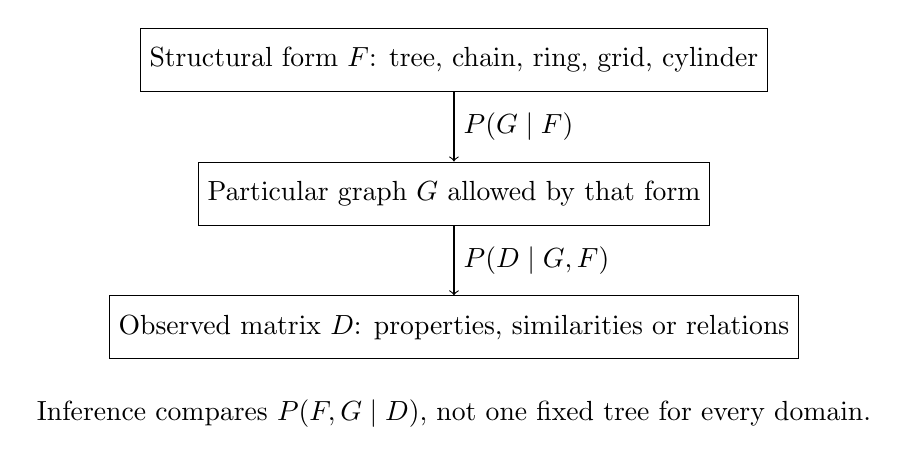
\begin{tikzpicture}[x=1cm,y=1cm]
\node[draw,minimum width=6.2cm,minimum height=.8cm,align=center] (form) at (0,4) {Structural form \(F\): tree, chain, ring, grid, cylinder};
\node[draw,minimum width=6.2cm,minimum height=.8cm,align=center] (graph) at (0,2.3) {Particular graph \(G\) allowed by that form};
\node[draw,minimum width=6.2cm,minimum height=.8cm,align=center] (data) at (0,.6) {Observed matrix \(D\): properties, similarities or relations};
\draw[->] (form.south)--node[right]{\(P(G\mid F)\)}(graph.north);
\draw[->] (graph.south)--node[right]{\(P(D\mid G,F)\)}(data.north);
\node[align=center] at (0,-.5) {Inference compares \(P(F,G\mid D)\), not one fixed tree for every domain.};
\end{tikzpicture}
\caption{Native explanatory diagram of the hierarchy in source Figure~3.3.
It preserves form, structure and data as different levels without pretending
to reproduce the source's fitted animal, voting, color, face or city data.}
\label{fig:p19-bci-hierarchy}
\end{figure}

Source Figure~3.3 says that an algorithm \emph{attempts} to find
a high-posterior form/graph pair; it does not prove that every search finds
the global optimum.

The examples retain different data types: animal features favor a tree;
judges' voting patterns a linear ordering; color similarities a ring;
the source's two manipulated face dimensions a grid; and geographic
proximities a cylindrical organization analogous to latitude/longitude.
These are reviewed model demonstrations, not a controlled comparison
showing that human participants recovered all five representations or
that the selected form is uniquely true of every such domain.

\begin{hbtheorem}{thm:p19-bci-tree-count}{proved=annex:p19.bci.tree-count}{The tree restriction and its counting convention}
A set of \(n\geq2\) distinct objects has \(2^n\) subsets. A fixed
rooted full binary tree with those objects as its leaves has \(n-1\)
internal nodes, hence \(n-1\) distinct nonsingleton descendant-leaf clades.
Allowing just those clades supplies the restricted \(n-1\) candidate
concepts used in the source's comparison. Including singleton leaves gives
\(2n-1\) clades; literally counting edges gives \(2n-2\). Thus the
source's shorthand about branches requires an explicit candidate convention.
\end{hbtheorem}

The reduction illustrates an inductive constraint; it does not establish
that the fixed tree is the correct one, where it comes from, or that
every actual category is a clade. A restricted space that excludes the
data-generating structure cannot recover it by updating alone.

\section{Identifying priors and iterated learning}
\label{sec:p19-bci-iterated}

The chapter gives three routes to studying inductive constraints: comparing
prior-dependent predictions with task data; asking which priors would make
observed learning possible from the available information, including
linguistic corpora; and designing procedures intended to reveal priors.
Each depends on likelihood and response assumptions as well as the prior.
An explanation by one fitted prior is not proof that no alternative model
can explain the observations.

Iterated learning supplies the third route. One learner receives data,
selects a hypothesis and produces data for the next learner. The 2007
formal paper distinguishes sampling from a posterior from selecting a
maximum-posterior hypothesis. Merely using Bayes's identity does not fix
that selection rule. Stationarity and convergence are also different
claims; convergence requires mixing conditions
\cite[pp.~29--30]{GriffithsTenenbaumKemp2012BayesianInference}
\cite[pp.~444--447,453--457,459--460]{GriffithsKalish2007IteratedAgents}.

\begin{hbtheorem}{thm:p19-bci-iterated}{proved=annex:p19.bci.iterated}{A complete finite posterior-sampling guarantee}
Assume the finite model in \cref{def:p19-bci-model}, with
\(\pi(h)>0\) and \(L(d\mid h)>0\) for every \(h,d\).
All learners have the same prior/likelihood. Given hypothesis \(j\),
produce \(d\) from \(L(d\mid j)\), then sample the next hypothesis
\(i\) from \(q_d\). Define the column-stochastic transition matrix
\[
 Q_{ij}=\sum_{d\in\mathcal D}q_d(i)L(d\mid j).
\]
This orientation matches the original's destination-first indices.
The prior is stationary, \(Q\pi=\pi\), and every initial hypothesis
distribution converges to it. The generated-data distribution converges
to \(m\). The annex gives an explicit geometric contraction bound.
Replacing posterior sampling by MAP selection need not preserve the prior;
removing mixing conditions can preserve the initial hypothesis indefinitely.
\end{hbtheorem}

\subsection{The original function-learning experiment}

Kalish, Griffiths and Lewandowsky's 2007 experiment supplies an actual
human task record rather than assuming that participants are the agents
in the theorem. It recruited 288 undergraduate psychology students at the
University of Louisiana at Lafayette for partial course credit: 72 per
initial-function condition, organized into eight families of nine learners
per condition, hence 32 transmission families. Ages, gender composition,
probability sampling, a prospective power calculation and a random
condition-assignment procedure are not reported
\cite[pp.~290--291]{KalishGriffithsLewandowsky2007Iterated}.

Participants worked individually in sound-attenuated booths. An input
\(x\) was displayed as a blue bar, and an unmarked mouse-controlled
slider set a red response bar representing \(y\). Values ran from 1
to 100. Initial targets were positive linear \(y=x\), negative linear
\(y=101-x\), a nonlinear U-shaped function, or random one-to-one
pairings. Fifty input values were drawn for training; values were rounded
to integers. The 50-item test used 25 training inputs and 25 previously
unused inputs. Each learner's test responses became the next learner's
training targets, without personal contact or disclosure of that transmission
role.

Training trials gave feedback. Accuracy within five units of target
yielded a one-second study interval; an error produced a tone, required
matching the feedback bar and yielded two seconds of study, followed
by a two-second blank interval. Test trials had no feedback. Thus initial
function conditions and the gradually changed target sets were defined,
but learners' errors also affected feedback exposure. These conditions
must not be replaced by a claim of unrestricted natural cultural transmission.

Twenty-eight of the 32 families reached a positive linear response
function in a few generations. Three ended with a negative linear function,
and one had not converged by the ninth generation. Eleven families
transmitted a negative linear function at least once. The quantitative
summary uses each learner's correlation with \(y=x\), summarized by
medians across families because negative-function outliers affect means.
No table of coefficient values, confidence intervals for the human
correlations or inferential test is supplied. The article's 1,000-chain
simulation intervals concern Bayesian agents, not 1,000 human participants
\cite[pp.~291--292, fig.~3]{KalishGriffithsLewandowsky2007Iterated}.

Source Figure~3.2 displays selected positive-convergence trajectories.
The primary paper's text calls its examples representative, whereas its
figure caption calls the rows randomly drawn; no selection protocol resolves
that difference. In either case, the displayed rows are not all 32 families.
The original also includes the negative outcome and explicitly states
that substantially more data would be needed to confirm stationarity and
map the distribution. These qualifications prevent upgrading a tendency
in the study into universal convergence or proof that human learners
sampled their mathematical posteriors.

The prior may encode acquired or domain-general constraints; a transmission
pattern does not show that a bias is innate or specific to language.
The paper's two notes preserve those limitations. Function learning is
the measured task. Generalization to language, legends or norms remains
an interpretation requiring separate evidence, not an additional outcome
measured in these students.

\section{Hierarchies, causal schemas and abstraction}
\label{sec:p19-bci-hierarchies}

The source's hierarchical Bayesian account puts priors on structures and
on the higher-level constraints determining those structures. Learning
can then occur at several levels, with higher-level knowledge constraining
lower-level inferences while evidence below informs the higher levels.
This does not eliminate assumptions: the possible hyperstructures,
hyperpriors, generative factors and search procedures still must be supplied.

Figure~3.4 is a computational illustration with sixteen hypothetical
condition variables: six disease nodes and ten symptom nodes. A two-level
network/data model with a weak structural prior is contrasted with a
three-level class-schema/network/data model favoring class~\(C_1\)
to class~\(C_2\) links. The caption reports little specific-network
learning at 20 records and spurious links at 80 in the two-level model;
the three-level model learns the class-level organization at 20 and
nearly recovers the illustrated network at 80. A 1,000-record comparison
is mentioned but not shown. Those record counts index the model's data,
not a clinical trial or a demonstrated human sample size requirement
\cite[pp.~30--32, figs.~3.3--4]{GriffithsTenenbaumKemp2012BayesianInference}.

The chapter uses these results to motivate learning a framework before
all its specific relations. The blessing-of-abstraction explanation is
that a higher-level constraint pools evidence from many lower-level
variables. It is a property of particular model structures, not a theorem
that every abstraction is learned faster or that adding layers always
improves predictive accuracy. The source contrasts this approach with
selected nativist and bottom-up associationist accounts. Its stronger
suggestion that only HBMs suit early learned abstraction is an argumentative
assessment, not an independently established exclusion of every rival
developmental mechanism.

The historical Linnaeus tree and Mendeleev periodic-structure examples
illustrate discovering a form rather than fitting parameters within a
single predetermined form. They are not reconstructions of those
discoveries by a human subject model. The available form grammar limits
what a computational learner can discover; calling the process structure
discovery does not make an unprovided representation available.

\section{Connections, open problems and consultation}
\label{sec:p19-bci-use}

The source relates exemplar/prototype categorization to density estimation,
rational categorization to nonparametric Bayesian methods, causal induction
to graph structure/strength distinctions, and learning/perception to
conditioning, multisensory integration and perceptual organization.
These correspondences create hypotheses and mathematical tools; they
do not establish an identical cognitive mechanism across all those tasks.
Its later examples include single-sample decision tradeoffs, Church-style
probabilistic programs, relational and feature-discovery models. This
chapter does not give each named algorithm's complete correctness or
optimality proof, and the single-sample advantage is conditional on a
particular gain/time tradeoff rather than a universal prescription
\cite[pp.~31--33]{GriffithsTenenbaumKemp2012BayesianInference}.

The conclusion seeks to move beyond empiricism/nativism, domain-general/
domain-specific and symbol/statistics dichotomies by asking how learned
representations and constraints cooperate. It identifies developing
mechanistic accounts and explaining rapidly learned structured knowledge
as open research directions. A common Bayesian language does not make
the model-building or empirical-validation problems disappear.

\begin{hbmethod}{def:p19-bci-assessment}{Assess a Bayesian cognitive account}
State the inference question, the hypothesis representation, data and
observation mechanism. Give the prior, likelihood and posterior-to-response
rule; check evidence support rather than dividing by zero. Preserve the
source's representation variant instead of treating all models as one formula.

Identify the explanatory level and claim: conditional mathematical identity,
normative comparison, descriptive fit, approximate algorithm or implementation.
Show which evidence could distinguish competing models with similar outputs.
Do not use a computational fit as its own mechanism test.

Map every human outcome to its population, task, instructions, design,
measure, uncertainty, selection and dependence structure. Separate human
learners from simulations, medians from individuals and data records from
participants. State unavailable fields as unavailable.

For a rival comparison, hold the interpreted question and environmental
assumptions explicit. A changed task construal can explain a response
without answering the original task correctly. A heuristic comparison
needs a comparable treatment of structural constraints and flexibility.

Conclude at the justified scope: success on a particular prior-sensitive
task, a conditional convergence theorem or a model demonstration is not
universal Bayesian competence, guaranteed global search or current clinical
knowledge. Retain any source-level unresolved mechanism or empirical gap.
\end{hbmethod}

Successful cases are finite updating on supported evidence, the coin
prediction/diagnosis distinction, a declared tree restriction and the
posterior-sampling guarantee with its mixing assumptions. Failure cases
are selecting an omitted hypothesis, confusing likelihood with posterior,
inferring neural machinery from fit, assuming MAP transmission preserves
the prior, or reading selected positive trajectories as every family's
outcome. \Cref{sec:p15-bayesian-updating-prediction,sec:p15-bayesian-model-comparison}
supplies the general mathematical interfaces; \cref{def:p19-evidence-record}
supplies the empirical discipline. Neither substitutes for the source's
particular cognitive model, experiment or admitted boundary.

% ED26-BM-OHTR2012-6: full Morrison-Knowlton2012 methods treatment.
\chapter{Neurocognitive Methods in Higher Cognition}
\label{sec:p19-neurocognitive-methods}

Morrison and Knowlton distinguish mapping brain--behavior relationships
from using neural evidence to constrain competing cognitive theories.
Several mechanisms can reproduce a behavioral result; an additional
neural prediction can exclude some, provided the measurement and
the proposed brain/process bridge are defensible. Their chapter
surveys neuropsychology, structural and functional imaging, electrical
recordings, magnetic perturbation and computational models, emphasizing
prefrontal cognition and cooperative networks rather than a single
reasoning center \cite[chap.~6, pp.~67--89]{MorrisonKnowlton2012Methods}.

The source is a 2012 methods presentation. Its equipment ranges,
availability judgments and forecasts are dated descriptions, not
current clinical protocols. Nothing here recommends diagnosis,
treatment, stimulation or participant eligibility. Its own note~1
distinguishes \emph{cognitive neuropsychology}, the use of patient
dissociations to investigate cognition, from clinical neuropsychology's
psychometric appraisal. Note~2's diagnostic terminology supplies
the historical grouping used in the studies, not instructions for
classifying a person.

\section{What a neural observation can constrain}
\label{sec:p19-ncm-inference}

\begin{hbdefinition}{def:p19-ncm-claims}{Different neural and cognitive claims}
A \emph{correlate} covaries with a task, response or other measure.
\emph{Localization} assigns that measured signal or relevant contribution
to a specified anatomical site under a spatial model. \emph{Necessity}
claims that the function would fail without the relevant contribution
under the stated conditions. A \emph{perturbation effect} compares
outcomes under an intervention and its appropriate controls.
\emph{Mechanistic identification} additionally specifies the information
and operations by which the contribution supports behavior.

These are not synonyms. A region activated during a task need not
be necessary for its defining process; a necessary contribution can
be sensory, linguistic, motivational or motor rather than the
reasoning operation of interest. An intervention's effect also
does not establish that one local circuit is sufficient for the
whole behavior.
\end{hbdefinition}

The anatomical orientation in Figure~6.1 distinguishes frontal,
parietal, temporal and occipital lobes and narrower regions such
as dorsolateral and rostrolateral prefrontal cortex, DLPFC/RLPFC,
inferior frontal gyrus, IFG, and anterior temporal cortex, ATC.
Labels based on anatomy, historical investigators or functional
associations have different origins. The drawing locates names;
it does not demonstrate an exclusive function for every region.

Reverse inference moves from observed activity to the claim that
a particular cognitive process occurred. Forward evidence that
a process often activates a region is not enough: other processes
may activate it too, and the target process's prevalence in the
actual comparison matters. Baselines and task phases must also
be specified. A language-associated region active while premises
are read does not by itself show that subsequent deduction uses
a linguistic rule representation. This methodological distinction
develops the source's repeated warning about incidental processes,
not a clinical interpretation of a participant's scan.

\section{Patient cases and dissociation assumptions}
\label{sec:p19-ncm-patients}

The source contrasts historical localizationism with an aggregate
field account and recounts Broca's patients Leborgne and Lelong.
Modern inspection showed more extensive damage than the original
local description suggested. Similar presentations can also include
grammatical comprehension deficits, motivating an agrammatism
interpretation rather than a simple production/comprehension split.
The lesson concerns changing behavioral characterization and lesion
mapping, not diagnosing aphasia from one task
\cite[pp.~68, 72 and figs.~6.1--6.2]{MorrisonKnowlton2012Methods}.

\begin{hbdefinition}{def:p19-ncm-dissociation}{Single and double dissociation as evidence patterns}
A single dissociation has impaired performance on one function
with another relatively spared. A double dissociation adds the
complementary profile: another case or group is relatively impaired
on the second while sparing the first. Figure~6.2 illustrates
the two profiles. Two cases with the same production-impaired
profile do not alone establish a double dissociation.

Interpreting the pattern requires comparable task sensitivity,
appropriate control performance and a model of the effects of
damage. Unequal task difficulty, shared resource demands, disconnection,
compensation and different strategies can complicate the inference.
An observed dissociation constrains a theory; it does not automatically
prove anatomically isolated independent modules.
\end{hbdefinition}

Skill learning with poor memory for practice episodes motivates
the source's declarative/procedural-memory contrast. For reasoning,
its frontal/temporal patient comparison separates relational integration,
interference control and access to semantic knowledge. Single-relation
matrix tasks can be spared while tasks combining changes across
rows and columns are impaired in the frontal group. Temporal-group
semantic deficits can instead affect familiar materials while
arbitrary-content reasoning remains relatively possible. These are
chapter reports attributed to Waltz, Morrison, Krawczyk and related
studies, not prevalence estimates for all neurological populations
\cite[pp.~68, 72--73]{MorrisonKnowlton2012Methods}.

Damage location and extent vary; focal unilateral lesions may
permit compensation, and degenerative groups are neither random
lesions nor homogeneous circuit removals. Structural volume--behavior
associations help characterize these differences but do not themselves
make a damaged site necessary for one unique computation. The
source's semantic/arbitrary-circuit interpretation therefore remains
an explanatory proposal requiring task-sensitive comparisons.

\section{Measurement families and the source's comparative table}
\label{sec:p19-ncm-measurements}

Table~6.1 compares thirteen methods across lag, acquisition timing,
spatial scale, advantages and constraints. Those fields answer
different questions. A millisecond sampling interval is not a
millisecond hemodynamic response, and it is not a rate expressed
in hertz. Anatomical image resolution is not identical to the
resolution of functional source inference.

\begin{center}
\begin{tabular}{@{}p{0.27\textwidth}p{0.29\textwidth}p{0.36\textwidth}@{}}
\toprule
Source method & Recorded information & Main inferential limitation\\
\midrule
Patient neuropsychology & Behavioral deficit/spared-function profiles,
with damage characterization & Nonrandom heterogeneous damage,
compensation and task sensitivity.\\
CT & Structural X-ray reconstruction & Anatomy does not directly
measure an ongoing cognitive operation.\\
Structural MRI/VBM & Tissue contrast, thickness and normalized regional
volume comparisons & Segmentation, registration and group comparisons
require models; volume is not a synapse count.\\
DTI & Directional water-diffusion measurements & Tissue/connectivity
interpretation is indirect, not direct observation of messages.\\
Single/multi-unit recording & Local electrode activity & Invasive,
restricted sites and species/task transfer.\\
ECoG & Electrical activity at selected cortical sites & Selected
participant/site coverage, volume conduction and pathology.\\
EEG/ERP/ERO & Scalp voltages, time-locked means or frequency analyses
& Excellent timing does not uniquely locate a generator or identify a process.\\
PET & Tracer-related metabolic/receptor measurements & Indirect neural
interpretation, coarse timing and invasive tracer procedures.\\
fMRI & BOLD hemodynamic measurements & Delayed vascular signal,
baseline/analysis dependence and no necessity proof from activation.\\
MEG & Magnetic fields associated with neural currents & Source-model
ambiguity remains despite different spatial sensitivity from EEG.\\
fNIRS/EROS & Hemoglobin-related optical measures/fast optical scattering
& Different physiological targets; superficial coverage and model-dependent inference.\\
TMS & Perturbation and subsequent behavior/recording & Controls,
timing, field spread and network consequences limit localization.\\
\bottomrule
\end{tabular}
\end{center}

This is an editorial reconstruction of the comparison, not a new
benchmark. The original table's spatial orders range from
10 micrometers--1 millimeter for unit recording through roughly
1--10 millimeters for ECoG, optical methods, TMS and lesion characterization,
to roughly 10--100 millimeters for EEG/MEG, explicitly questioned
there. Structural/fMRI entries have broad millimeter--decimeter
ranges; PET is listed at centimeter--decimeter scale. They are
2012 approximate table entries, not guarantees of cognitive localization.
Its fMRI acquisition intervals are 250 milliseconds--1 second,
with 1--2-second onset lag and a response developing over seconds;
fNIRS also has a hemodynamic lag despite fine sampling. The EROS
entry lists about 100 milliseconds of lag. The table's question
marks and unavailable timing fields remain uncertainty, not zero
\cite[table~6.1, pp.~69--71]{MorrisonKnowlton2012Methods}.

\subsection{Structural methods}

CT and then MRI made damage accessible without waiting for a
postmortem examination. MRI supports tissue contrast, volumetry
and cortical-thickness analysis; VBM introduces spatial normalization
and voxelwise comparisons. The source's developmental reasoning
example associates adolescent prefrontal gray-matter reductions
with behavior. It suggests synaptic/connectivity change, but MRI
volume alone does not demonstrate pruning or prove its causal
effect on reasoning. DTI measures diffusion characteristics that
can inform white-matter models; it is not a direct assay of
fiber integrity or information flow. These distinguish measured
quantities from biological interpretations
\cite[pp.~73--74]{MorrisonKnowlton2012Methods}.

\subsection{Electrical measurements and working-memory control}

Local unit recordings can constrain when activity occurs at a
sampled site. The source's macaque delayed-match example separates
sample presentation, maintenance delay and response. Its cortical-
cooling comparison supports an interaction account in which
prefrontal activity helps maintain posterior representations, rather
than a simple isolated storage buffer. Species, task and intervention
conditions constrain transfer to human reasoning
\cite[pp.~74--75]{MorrisonKnowlton2012Methods}.

ECoG provides selected human cortical recordings; the chapter's
examples come from clinically obtained access rather than a
random sample of intact brains. Cross-frequency coupling motivates
communication/binding hypotheses, but correlated phase and power
do not count neurons or uniquely establish what content is bound.
Scalp EEG is a mixed electrical signal, not separate spike trains
from identified neurons. Its spatial inverse problem permits
multiple source configurations producing similar recorded voltages.

ERPs average measurements time-locked to a stimulus or response.
Figure~6.3 labels illustrative positive/negative peaks P1, N1, P2, N2, P3;
the sign convention, reference, latency and task must be known before
a component is interpreted. Averaging can reduce non-time-locked
noise under suitable assumptions, but systematic artifacts and
trial-to-trial timing variation do not disappear by definition.
Event-related oscillation analyses retain information about frequency,
phase and time that an average waveform can obscure. A Fourier
or wavelet transformation does not directly estimate the number
of neurons participating in each cognitive process.

The source's P30 auditory-click patient comparison suggests sensory
gating by DLPFC. Its insight examples describe alpha activity
before a solution and gamma activity near the reported answer;
the prepared-mind example concerns prediction before problem
presentation. These are different contrasts, not an identical
neural signature of insight. Except for the separately acquired
Vogel anchor below, the chapter does not supply each original
sample, trial denominator, effect interval or complete analysis.
Interpretations as gating or semantic integration remain competing-
mechanism claims, not uniquely identified processes
\cite[pp.~75--77]{MorrisonKnowlton2012Methods}.

\subsection{The actual Vogel 2005 anchor}

Vogel and colleagues studied 15 neurologically normal college
students aged 19--28 in each of three experiments, with 200--240
trials per condition per participant. These are participants and
within-person trials, not hundreds of independent people. A
visual-memory estimate supplied a median split into
high/low groups; group membership was not randomized
\cite[pp.~500--503]{VogelEtAl2005Selection}.

Experiment~1 used a cued left/right hemifield. Participants remembered
red rectangles' orientations and judged whether a test array one
second later changed. Conditions were two red items, four red items,
or two red plus two irrelevant blue items. The EEG outcome was
\emph{contralateral delay activity}, CDA, from posterior sites;
the original paper measures a lateralized difference during
300--900 milliseconds after array onset. It is not the contingent
negative variation, CNV, as named in the 2012 survey. Twenty-two
electrode sites were recorded, with blink/large-eye-movement trial
rejection. Missing trials and retained averages therefore matter.

Distractor-present CDA was nearer the two-item condition in the
high group and the four-item condition in the low group. The
filtering-score/capacity correlation was \(r=0.69\), reported
\(p<0.001\); no confidence interval is given. Experiment~2
used easier location selection and reported \(r=0.62\),
\(p<0.001\). Experiment~3 introduced a second array after
500 milliseconds and distinguished appending red items from
excluding green ones; its reported relation was \(r=0.57\),
\(p<0.01\). Appending was relatively preserved across groups
while exclusion differed. Changed task versions support a bounded
generalization of the filtering interpretation, not a universal
capacity theory \cite[pp.~500--502]{VogelEtAl2005Selection}.

\begin{hbdefinition}{def:p19-ncm-scores}{The primary's capacity and filtering measures}
For the capacity estimate the paper uses \(K=S(H-F)\), where
\(S\) is array size, \(H\) the hit proportion and \(F\)
the false-alarm proportion. This is a supplied task model and
estimator, not a direct count of an individual's neural storage slots.

In the separate filtering-score context the source reuses \(F\)
for four-item mean CDA amplitude, \(D\) for distractor-present
amplitude and \(T\) for two-item amplitude. Its published score is
\[
                       \alpha=\frac{F-D}{F-T}.
\]
Here those symbols are amplitudes, not response proportions.
The score measures the distractor condition's relative position
between two physiological comparison conditions.
\end{hbdefinition}

\begin{hbtheorem}{thm:p19-ncm-score}{proved=annex:p19.ncm-score}{The actual filtering-score range and boundary}
For real amplitudes with \(F\ne T\), the score equals one
when \(D=T\), zero when \(D=F\), and lies in \([0, 1]\)
exactly when \(D\) lies between \(T\) and \(F\), including
endpoints. If \(F=T\), the ratio is undefined. For the separate
capacity formula with \(S>0\) and \(H, F\in[0, 1]\),
\(-S\leq K\leq S\), and nonnegative \(K\) additionally
requires \(H\geq F\). Neither formula by itself establishes
that the reported score equals an intrinsic cognitive capacity.
\end{hbtheorem}

The primary explicitly allows filtering scores outside zero--one
mathematically while reporting none in its observations. Its
interpretation is that capacity differences need not \emph{simply}
reflect storage space: allocation efficiency can contribute.
The 2012 survey's stronger claim that the groups do not differ
in capacity is not adopted. Nor does a posterior CDA association
localize its causal source uniquely to PFC. The primary proposes
a prefrontal bias signal as plausible, not as an intervention result
\cite[p.~502]{VogelEtAl2005Selection}.

\section{Hemodynamics, optics and network modeling}
\label{sec:p19-ncm-hemodynamics}

PET uses tracer-related measurements and fMRI uses blood-oxygenation-
dependent, BOLD, signal. Both require a physiological bridge from
neural activity to the measured quantity. Tracer choice can address
different metabolic/receptor questions; it does not make PET a
direct measure of every neurotransmitter's firing. Figure~6.4
illustrates transient oxygen demand followed by a vascular response.
The increased positive-BOLD phase has reduced relative
deoxyhemoglobin following that response. The displayed curves
are explanatory schematics, not
new participant data \cite[pp.~77--78]{MorrisonKnowlton2012Methods}.

Event-related fMRI can separate modeled phases and intermix trials,
but blood dynamics blur timing. Removing error trials changes
the estimand; it does not reconstruct an unobserved error-free
mind. Activity varies with logical form, meaningful content, belief
conflict and perceptual demands. The source contrasts arbitrary
conditional problems, meaningful bicycle/weather problems and
transitive spatial relations. Its conditional examples are not
categorical syllogisms merely because the survey uses that label.
Every inference benchmark requires its actual premise interpretation.

The survey does not find unequivocal imaging support for mental
logic over mental models or vice versa. The premise that a
rule theory must use linguistic cortex and a model theory right
visuospatial cortex is itself a bridge hypothesis. Separating
premise reading from solution phases can constrain it, but a
region's temporal contrast does not prove a unique representational
format. The claim is about possible separation of language
processing and reasoning, not reasoning being independent of thought
\cite[pp.~78--79]{MorrisonKnowlton2012Methods}.

The Sonty language-network example contrasts semantic with letter
matching in patients and controls. Poorer behavior occurred without
simply reduced local activation; a fitted dynamic-causal-modeling,
DCM, connectivity difference supplied another account. The modeled
coupling/performance association does not prove that reduced
communication uniquely caused the deficit. DCM estimates depend
on a generative model, selected regions, connections and comparison;
it is not direct observation of individual synapses. Functional
connectivity based on correlated BOLD is likewise distinct from
directional causal influence or an anatomical tract
\cite[pp.~80, 84]{MorrisonKnowlton2012Methods}.

MEG measures magnetic fields associated with neural currents.
Its different field/source sensitivities can constrain localization
but do not remove the inverse problem. The source's child/adult
n-back example permits equal behavioral performance with different
signals; neither identical behavior nor different signals alone
settles which complete mechanism is used.

fNIRS estimates changes involving oxy/deoxyhemoglobin, with rapid
acquisition but delayed hemodynamics. EROS targets faster optical
scattering rather than that same blood response. Both have
superficial-coverage limitations in the source. The chapter's
48-participant fNIRS belief-bias example crosses short/long time
with congruent/incongruent problems and associates right IFG
activity with some accuracy contrasts. Congruence here should
separate logical validity from conclusion believability; factual
truth alone is not logical validity. The source supplies a sample
count and directional survey but no full original effect/interval/
design record. An activity correlation does not establish the
claimed inhibition mechanism or necessity
\cite[pp.~80--81]{MorrisonKnowlton2012Methods}.

\section{TMS: intervention with limited localization}
\label{sec:p19-ncm-tms}

TMS changes electromagnetic conditions rather than only recording
a signal. The relevant evidence compares behavior under the
intervention with suitable conditions controlling site, timing,
sound, sensation, expectation and task demands. Perturbation may
alter linked networks or other processes required to perform
the task. Enhancement and disruption are not interchangeable
with permanent focal damage, or with sufficient activation of
one reasoning module.

The source's right-IFG follow-up reports increased belief-bias
under repetitive TMS on incongruent trials. This supports a
contribution under the studied task/control conditions, not a
deduction that IFG contains only a belief-inhibition operation.
The chapter does not supply the complete original sample,
stimulation/control/effect/uncertainty record. It also notes
surface accessibility and the difficulty of testing cortical--
subcortical interactions this way. The treatment discussion and
categorical eligibility statements in its dated table are not
adopted as current clinical guidance or an intervention recommendation
\cite[pp.~81--82]{MorrisonKnowlton2012Methods}.

\section{A worked prefrontal/semantic comparison}
\label{sec:p19-ncm-analogy}

The separately acquired Morrison 2004 primary studied picture and
verbal analogies in frontal/temporal FTLD groups and age/education-
matched controls. Experiment~1 included 7 frontal patients,
6 temporal patients and 8 controls; experiment~2 included 7, 6
and 10 respectively. These are the actual task-specific samples,
not randomly assigned lesions or a representative population.
Selection included abnormal imaging and the source's MMSE
threshold. That characterizes recruitment; it is not a diagnostic
rule offered here \cite[pp.~267--268]{MorrisonEtAl2004Analogy}.

Ten picture pairs permitted a salient feature match or a relational
match. Participants inspected each for ten seconds, then indicated
what went with a pointed-out object; there were no practice
examples and one predetermined order. Both patient groups made
fewer relational and more featural choices than controls. Frontal
relational choices more often benefited from perceptual alignment.
That pattern leaves working-memory integration, inhibition and
semantic access as competing contributors, not one uniquely located
faculty \cite[pp.~262--264, 267]{MorrisonEtAl2004Analogy}.

Experiment~2 used 24 two-choice verbal analogies selected from
200 candidates with association/difficulty norms from separate
UCLA undergraduate samples, 150 for association and 54 for
difficulty. A semantic-facilitation index, SFI, contrasted normalized
association of the correct versus distractor pair. Positive,
neutral and negative conditions used thresholds around plus/minus
0.3. The source's play:game::give:? example pits \emph{party}
against the more strongly associated \emph{take}. Random problem
order followed five practice items. Outcome was answer accuracy,
not a direct neural measure or proof of the association's causal origin.

Frontal-group accuracy was selectively poorer when association
favored the distractor; temporal-group accuracy was more uniformly
reduced. The source reports the frontal differential contrast
\(F(1, 19)=5.0\), \(p=0.04\), while the analogous temporal
contrast was not detected. Figure~4 uses one-standard-error bars;
no confidence interval or participant-level reanalysis is supplied.
The reported analysis unit/denominator must not be inferred solely
from the degrees of freedom or trial count. Small clinical groups,
heterogeneous damage, item selection and fixed-order picture testing
limit generalization \cite[pp.~265--268]{MorrisonEtAl2004Analogy}.

Its LISA simulation used 40 trials per problem type and changed
mapping learning/inhibition to model frontal deficits versus semantic
connections for temporal deficits. It reproduced qualitative patterns,
with tested parameter assumptions rather than measured neuronal
values. Neither frontal manipulation alone reproduced the selected
pattern in that model. This is a useful competing-mechanism
boundary, not independent proof that actual lesions change precisely
those parameters or that no other architecture can explain the
results \cite[pp.~266, 268--270]{MorrisonEtAl2004Analogy}.

\section{Neurocomputational bridges and the prefrontal alternatives}
\label{sec:p19-ncm-models}

ACT-R's production architecture and its task-specific assumptions
can predict behavior; associating its representation, retrieval
and response functions with regions introduces an additional
bridge. The chapter's Tower-of-Hanoi example is an external
model/imaging account, not an acquired executable ACT-R instance.
Behavioral fit alone is not neural validation.

Figure~6.5 develops LISA's proposed bridge in five panels: distributed
semantic representations and conjunctive long-term codes; dynamic
working-memory proxy/role-binding units; candidate retrieval based
on integrated activation; synchronized driver/recipient mapping
through rapidly learned links; and increased anterior-prefrontal
involvement for higher-order relations. Its lover/loved example
binds the two roles in distinct temporal phases rather than mixing
the object features into an unordered list. DLPFC maintenance,
IFG competition control, ATC/hippocampal representation and
RLPFC mapping assignments are hypotheses. Observed rhythmic
activity alone does not verify each proxy unit, Hebbian connection
or synchrony-based relational binding
\cite[pp.~82--84 and fig.~6.5]{MorrisonKnowlton2012Methods}.

The source distinguishes crystallized knowledge from fluid reasoning
and surveys task-complexity-dependent recruitment. It does not
turn a scan into an intelligence diagnosis. Common lateral
prefrontal/anterior-cingulate recruitment can reflect a shared
control operation or flexible support of several operations.
The hierarchical proposal distinguishes sensory-response, context
and episodic-memory demands; medial/orbital social/emotional
associations have other comparisons. RLPFC integration and
abstraction accounts remain explicit alternatives. A region's
name or greater activation does not decide between them
\cite[pp.~84--85]{MorrisonKnowlton2012Methods}.

The chapter's three future priorities are cortical connectivity,
integration of spatial/temporal measurement, and neurally plausible
computational hypotheses. Convergence of methods is valuable when
their independent assumptions and predicted contrasts constrain
one another. Repeating one localization assumption in several
analyses is not independent corroboration.

\section{Consultation and related evidence interfaces}
\label{sec:p19-ncm-use}

Goel's Chapter~\ref{sec:p19-rationality-1-4} offers a particular
reasoning-systems account, not the present chapter's whole methods
survey. Knauff's Chapter~\ref{sec:p19-rationality-13-3} separates
visual detail, spatial organization and task performance; an occipital
signal need not identify pictorial reasoning. Cognitive representation
in Chapter~\ref{sec:p19-cognitive-knowledge-representation} supplies
encoding/process distinctions that a neural bridge must preserve.
These are complementary interfaces, not duplicate source credits.

\begin{hbmethod}{def:p19-ncm-use}{Match the neural method to the inference actually needed}
Specify the population, task, behavioral measure and proposed mechanism.
Name the neural observable, physiological bridge, baseline, time phase,
spatial/source model and processing steps. Distinguish acquisition
timing from physiological lag and analysis resolution.

For patient evidence characterize lesion/degeneration and spared
performance, including sensitivity and compensation alternatives.
For activation evidence test selectivity and competing processes
before reversing the inference. For perturbation state intervention,
controls, network effects and the task component actually changed.
For connectivity specify observed correlation versus model-based
directional coupling and what could distinguish other models.

Construct the task-specific evidence record in
Method~\ref{def:p19-evidence-record}. Keep participants, trials,
conditions and model runs as distinct denominators. A nonsignificant
difference is not proof of equality; a successful fitted simulation
is not a unique brain mechanism. State transfer and replication
limits and preserve unresolved source-study boundaries.
\end{hbmethod}

The useful success case combines retained behavioral contrasts
with method-specific neural predictions and an actually controlled
perturbation or dissociation. Failure cases include reading capacity
alone from a mixed ERP, inferring a specific thought from generic
PFC activation, calling correlated BOLD a proved causal pathway,
or transferring one patient task to all reasoning. The source
provides tools for distinguishing these questions, not a universal
neural verdict of rationality.

\index{neurocognitive methods}
\index{neural evidence!reverse inference}
\index{neuropsychology!single and double dissociation}
\index{EEG!ERP and oscillations}
\index{fMRI!BOLD and inference}
\index{TMS!perturbation and localization}
\index{prefrontal cortex!competing mechanisms}

